\documentclass{ctexbook}
%句点. 
\usepackage{xparse,amsmath,physics,amssymb,amsopn}%math
\usepackage{geometry,fontsize,setspace,xcolor,fancyhdr}%typesetting
\usepackage{tikz}%drawing
\usepackage[OT2,OT1]{fontenc}%Russian
\usepackage[colorlinks=true]{hyperref}%tableofcontents
\usepackage{pdfpages}
\geometry{a4paper,top=1.27cm,bottom=1.27cm,inner=2.54cm,outer=1.27cm}
\allowdisplaybreaks[4]
\DeclareMathOperator{\arsinh}{arsinh}
\DeclareMathOperator{\arcosh}{arcosh}
\DeclareMathOperator{\artanh}{artanh}
\DeclareMathOperator{\arcoth}{arcoth}
\DeclareMathOperator{\arsech}{arsech}
\DeclareMathOperator{\arcsch}{arcsch}
\DeclareMathOperator{\sgn}{sgn}
\newcommand{\e}{\mathrm{e}}
\newcommand{\im}{\mathrm{i}}
\newcommand*{\dif}{\mathop{}\!\mathrm{d}}
\newcommand{\m}{\,\mathrm{mod}\,}
\everymath{\displaystyle}
\setcounter{secnumdepth}{2}
\setcounter{tocdepth}{1}
\begin{document}
\large
\setstretch{1.5}
\setlength{\parskip}{0.4em}
{
\includepdf[]{Cover.pdf}
\thispagestyle{empty}
}
\frontmatter{
\pagestyle{headings}
\chapter{序}
本书为\textit{cppHusky}的二〇二三年年礼. \par
这是一本以方法为导向, 按难度来分级的不定积分题集. 这里收集了大量我在不定积分学习过程中认为有价值的习题. 笔者致力于将其打造为适合各层次不定积分学习者可用的习题集. 它适合于大学考研应试学生和对不定积分感兴趣的数学爱好者. \par
笔者吸收了吉米多维奇习题解集的风格来编撰这本习题集, 旨在让考研学生掌握必需的不定积分解题方法, 让不定积分爱好者了解更多相关方法, 拓宽知识面. \par
由于这本书采用了难度分级体系, 学习者可以选择自己适合的难度来进行训练. \par
作为习题集, 本书还有许多附加的实用功能. 笔者会在许多题目之后加入批注和同类题目索引, 也会在附录中提供不定积分类型题的讲义. \par
希望本书的每一个读者都能共借助这本书, 使自己的不定积分水平更上一层楼. \par
\section*{内容结构与格式约定}
\begin{itemize}
\item\textbf{难度分级系统}: 所有题目分七个难度等级, 从一级开始难度递增. 题目难度的划分标准为使用的方法 (越高级越难) 和计算量 (越复杂越难) , 前者为主要标准. 
\item\textbf{题目编号体系}: 分两个阶段进行. 内容扩充阶段使用随机编号, 成型阶段统一改为顺序编号. 随机标号的格式为“R”+难度分级对应的阿拉伯数字1位+随机数字3位; 顺序编号的格式为“T”+难度分级对应的阿拉伯数字1位+顺序数字3位. 
\item\textbf{编号标示方案}:根据题目所采用的方法, 分为“考研必会”和“其它”两类, 题号分别以红色和黑色标示. 红色编号对应的题目是考研110分水平必会的, 全部集中在一级题目至三级题目的范围内. 
\item\textbf{批注索引系统}: 以楷体字附于某些题目的解答之后, 主要为积分经验的总结和同类型、同方法题目的索引. 部分内容会索引到附录部分, 建议读者参照学习. 
\item\textbf{附录讲义系统}: 将有理函数积分、分部积分法等类型的讲义置于附录中. 这是笔者学习不定积分许久以来的方法汇总, 具备一定价值; 且用讲课的形式娓娓道来, 易于理解. 
\end{itemize}\par
本书遵循一套严格的排版方案, 排版美观清晰, 便于读者阅读. 
由于本书注重方法, 会存在同题多解的情况, 这也是提醒读者不要受限于单一的思路. 不定积分的方法灵活多样, 只有善于思考才能掌握精髓. \par
\begin{flushright}
\textit{cppHusky}\par
\end{flushright}
\newpage
\tableofcontents
\textbf{}
}\mainmatter{
\pagestyle{fancy}
\fancyhf{}
\renewcommand{\headrulewidth}{0pt}
\fancyhead[RO,LE]{\thepage}
\linespread{2}\selectfont
\chapter*{一级题目}
\addcontentsline{toc}{chapter}{一级题目}
\fancyhead[RE,LO]{\kaishu 一级题目}
{\color{red}【T1001】}$\int\qty(x+1)^{3}\dif{x}$\par
【解】
\begin{align*}
\int\qty(x+1)^{3}\dif{x}={}&\int\qty(x^{3}+3x^{2}+3x+1)\dif{x}\\
={}&\int x^{3}\dif{x}+3\int x^{2}\dif{x}+3\int x\dif{x}+\int\dif{x}\\
={}&\frac{x^{4}}{4}+x^{3}+\frac{3}{2}x^{2}+x+C
\end{align*}\par
{\color{red}【T1002】}$\int\qty(x+1)^{3}\dif{x}$\par
【解】令$\color{blue}u=x+1$, 则$\color{blue}x=u-1$, 所以
\begin{align*}
\int\qty(x+1)^{3}\dif{x}=\int u^{3}\dif{\qty(u-1)}=\int u^{3}\dif{u}=\frac{1}{4}u^{4}+C=\frac{1}{4}\qty(x+1)^{4}+C
\end{align*}\par
{\kaishu 读者倘若对{\color{red}【T1002】}的结果进行二项式展开, 就会发现$\frac{x^{4}}{4}+x^{3}+\frac{3}{2}x^{2}+x+\frac{1}{4}+C$和{\color{red}【T1001】}的结果是不同的. 然而, 这两个结果是等价的. 因为不定积分自带任意常数$+C$, 所以同一个不定积分得到的两个原函数之间可以相差任意常数. 再举个例子, $\ln{x}+C$和$\ln{\frac{x}{2}}+C$二者就是等价的. \par}
{\color{red}【T1003】}$\int\csc^{2}{\frac{x+1}{2}}\dif{x}$\par
【解】
\begin{align*}
\int\csc^{2}{\frac{x+1}{2}}\dif{x}={}&\int\csc^{2}{\frac{x+1}{2}}\dif{\qty(x+1)}\\
={}&2\int\csc^{2}\qty(\frac{x+1}{2})\dif{\frac{x+1}{2}}\\
={}&2\int\csc^{2}{u}\dif{u},\;{\color{blue}u=\frac{x+1}{2}}\\
={}&-2\cot{\frac{x+1}{2}}+C
\end{align*}\par
{\color{red}【T1004】}$\int x\e^{-x^{2}}\dif{x}$\par
【解】
\begin{align*}
\int x\e^{-x^{2}}\dif{x}=\frac{1}{2}\int\e^{-x^{2}}\dif{x^{2}}=-\frac{1}{2}\int\e^{-x^{2}}\dif{\qty(-x^{2})}=-\frac{1}{2}\e^{-x^{2}}+C
\end{align*}\par
{\kaishu 这两道题目是典型的凑微分问题. 凑微分的方法一般会用在包含复合函数的积分问题中, 比如说{\color{red}【T1004】}当中的$\e^{-x^{2}}$就是一个典型的复合函数. 换元的好处是把无关紧要的被复合部分给抽象出来, 能让做题人更容易判断整个被积函数的结构. 比如说{\color{red}【T1003】}当中的$\csc^{2}{\frac{x+1}{2}}$看上去就很臃肿, 而换元之后的$\csc^{2}{u}$就清晰很多, 可以一眼看出这是基本积分表里的积分. \par
至于如何凑微分呢, 笔者的建议是从复合函数的部分寻找思路, 然后去操作其它的部分. 就拿{\color{red}【T1004】}来说, 这里可以从复合函数$\e^{-x^{2}}$部分入手思考, 既然这里被复合的部分是$-x^{2}$, 那么应当在其它地方都凑出$-x^{2}$的结构, 这样才能把$-x^{2}$当作整体去参与积分运算. 于是凑微分的思路就是$x\dif{x}=\frac{1}{2}\dif{x^{2}}=-\frac{1}{2}\dif{\qty(-x^{2})}$. \par}
{\color{red}【T1005】}$\int\frac{1+\cos{x}}{x+\sin{x}}\dif{x}$\par
【解】
\begin{align*}
\int\frac{1+\cos{x}}{x+\sin{x}}\dif{x}=\int\frac{\dif{\qty(x+\sin{x})}}{x+\sin{x}}=\ln\qty|x+\sin{x}|+C
\end{align*}\par
{\kaishu 读者应当具备这种整体凑微分的思想, 笔者在这里将分子当成一个整体来凑微分. 这题难度不大, 主要原因是可操作空间太小, 容易想到整体凑微分的可能; 但有些复杂问题, 比如【T2032】, 如果缺少这类思路是可能走很多弯路的. \par}
{\color{red}【T1006】}$\int\sin{x}\sin{2x}\dif{x}$\par
【解】
\begin{align*}
\int\sin{x}\sin{2x}\dif{x}=2\int\sin^{2}{x}\cos{x}\dif{x}=2\int\sin^{2}{x}\dif{\sin{x}}=\frac{2}{3}\sin^{3}{x}+C
\end{align*}\par
{\kaishu 一般而言, 在处理三角函数积分时应当优先将各个角度统一, 这样才能够应用许多已知的解题方法. 统一角度常用的公式有二倍角公式、半角公式、和角公式与积化和差公式. 这些公式在附录B中都有介绍, 有需要的读者可以查看. \par
在本题中选择使用二倍角公式来统一角度, 这是因为二倍角公式不仅易记易用, 而且将被积函数变形之后只需要凑微分$\dif{\sin{x}}$就能够解决问题. \par}
{\color{red}【T1007】}$\int\sin^{2}{x}\dif{x}$\par
【解】
\begin{align*}
\int\sin^{2}{x}\dif{x}={}&\int\frac{1-\cos{2x}}{2}\dif{x}\\
={}&\frac{1}{2}x-\int\frac{\cos{2x}}{2}\dif{x}\\
={}&\frac{1}{2}x-\frac{1}{4}\int\cos{2x}\dif{\qty(2x)}\\
={}&\frac{1}{2}x-\frac{1}{4}\sin{2x}+C
\end{align*}\par
{\color{red}【T1008】}$\int\sin^{3}{x}\dif{x}$\par
【解】
\begin{align*}
\int\sin^{3}{x}\dif{x}={}&-\int\sin^{2}{x}\dif{\cos{x}}\\
={}&\int\left(\cos^{2}{x}-1\right)\dif{\cos{x}}\\
={}&\int u^{2}\dif{u}-\int\dif{u},\;{\color{blue}u=\cos{x}}\\
={}&\frac{1}{3}u^{3}-u+C\\
={}&\frac{1}{3}\cos^{3}{x}-\cos{x}+C
\end{align*}\par
{\kaishu 这类$\int\sin^{n}{x}\dif{x},\,\int\cos^{n}{x}\dif{x}$的问题有一个通用规律. \par
如果$n$是偶数, 则套用降幂公式$\sin^{2}{x}=\frac{1-\cos{2x}}{2},\;\cos^{2}{x}=\frac{1+\cos{2x}}{2}$来降低被积函数的幂次. 如果降到奇数次幂就可以用下面说的$n$为奇数的方法; 如果依然是偶数次幂, 还可以继续套用降幂公式. 这种类型的问题还有欧拉公式的解法, 可以参考{\color{red}【T3029】}. \par
如果$n$是奇数, 则凑微分成$\dif{\cos{x}},\,\dif{\sin{x}}$, 这样的话$\dif$左边剩下的是偶数次的, 可以套用$\sin^{2}{x}+\cos^{2}{x}=1$来进行变形, 这点在{\color{red}【T1008】}中已经有所体现了. \par}
{\color{red}【T1009】}$\int\frac{\dif{x}}{x^{2}+4}$\par
【解】令$\color{blue}x=2t$, 则$\color{blue}t=\frac{x}{2}$, 所以
\begin{align*}
\int\frac{\dif{x}}{x^{2}+4}=\int\frac{\dif{\qty(2t)}}{\qty(2t)^{2}+4}=\frac{1}{2}\int\frac{\dif{t}}{t^{2}+1}=\frac{1}{2}\arctan{t}+C=\frac{1}{2}\arctan{\frac{x}{2}}+C
\end{align*}\par
{\kaishu $x=at$这种换元并不怎么受重视, 但有些时候是会很有用的. 例如, 积分$\int\frac{\dif{x}}{x^{2}+a^{2}}\qty(a>0)$也是没有必要作三角换元的, 因为被积函数的结构很容易让人联想到$\int\frac{\dif{x}}{x^{2}+1}$的类型上来, 而这个积分是可以直接套用基本积分表来解决的. \par}
{\color{red}【T1010】}$\int\frac{x\dif{x}}{x^{4}+1}$\par
【解】
\begin{align*}
\int\frac{x\dif{x}}{x^{4}+1}=\frac{1}{2}\int\frac{\dif{x^{2}}}{\qty(x^{2})^{2}+1}=\frac{1}{2}\arctan{x^{2}}+C
\end{align*}\par
{\kaishu 这道题可以用裂项的做法, 但没必要做得如此复杂. 适当的凑微分能让问题得到简化. \par}
{\color{red}【T1011】}$\int\frac{1}{x^{2}+2x+1}\dif{x}$\par
【解】
\begin{align*}
&\int\frac{\dif{x}}{x^{2}+2x+1}=\int\frac{\dif{\qty(x+1)}}{\left(x+1\right)^{2}}=-\frac{1}{x+1}+C
\end{align*}\par
{\color{red}【T1012】}$\int\frac{\dif{x}}{x^{2}+2x+2}$\par
【解】
\begin{align*}
\int\frac{\dif{x}}{x^{2}+2x+2}&=\int\frac{\dif{\qty(x+1)}}{\qty(x+1)^{2}+1}=\arctan{\qty(x+1)}+C
\end{align*}\par
{\color{red}【T1013】}$\int\frac{\dif{x}}{x^{2}+2x}$\par
【解】
\begin{align*}
\int\frac{\dif{x}}{x^{2}+2x}\dif{x}={}&\int\frac{\dif{x}}{x\left(x+2\right)}\\
={}&\int\frac{1}{2}\qty(\frac{1}{x}-\frac{1}{x+2})\dif{x}\\
={}&\frac{1}{2}\int\frac{\dif{x}}{x}-\frac{1}{2}\int\frac{\dif{\qty(x+2)}}{x+2}\\
={}&\frac{1}{2}\ln\qty|x|-\frac{1}{2}\ln\qty|x+2|+C\\
={}&\frac{1}{2}\ln\qty|\frac{x}{x+2}|+C
\end{align*}\par
{\kaishu 这三题是有理函数积分的典型题目, 分别对应着三个基本公式的使用. 对于积分\\$\int\frac{\dif{x}}{ax^{2}+bx+c}$来说, 方法选取的关键在于观察分母二次多项式的根判别式$\Delta=b^{2}-4ac$. \par
当$\Delta=0$时, 可以直接配方解决; 当$\Delta<0$时, 配方过后分母还多出正常数, 要凑反正切形式 (可参考{\color{red}【T1009】}) ; 当$\Delta>0$时, 可因式分解并裂项. 裂项相关的内容在附录C.3、C.4和C.5中有所介绍, 读者可根据自己的水平选择学习. \par}
{\color{red}【T1014】}$\int\frac{x}{x-1}\dif{x}$\par
【解】
\begin{align*}
\int\frac{x}{x-1}\dif{x}={}&\int\frac{x-1+1}{x-1}\dif{x}\\
={}&\int\qty(1+\frac{1}{x-1})\dif{x}\\
={}&\int\dif{x}+\int\frac{\dif{\qty(x-1)}}{x-1}\\
={}&x+\ln\qty|x-1|+C
\end{align*}\par
{\color{red}【T1015】}$\int\frac{x^{3}}{x^{2}+1}\dif{x}$\par
【解】
\begin{align*}
\int\frac{x^{3}}{x^{2}+1}\dif{x}={}&\int\frac{x^{3}+x-x}{x^{2}+1}\dif{x}\\
={}&\int\qty(x-\frac{x}{x^{2}+1})\dif{x}\\
={}&\int x\dif{x}-\int\frac{x\dif{x}}{x^{2}+1}\\
={}&\frac{x^{2}}{2}-\frac{1}{2}\int\frac{\dif{x^{2}}}{x^{2}+1}\\
={}&\frac{x^{2}}{2}-\frac{1}{2}\ln(x^{2}+1)+C
\end{align*}\par
{\kaishu 这两题是有理函数假分式化为真分式的情形. 一般遇到被积函数是假分式的情形, 都要先将假分式分离成整多项式和真分式, 再分别处理整多项式的积分和真分式的积分. \par
关于凑配方法, 笔者建议使用附录C.6.1所介绍的凑配方法 (也正是这两题所用的) , 而不推荐使用待定系数法. 凑配的关键在于根据分子上的最高次项凑出能与分母进行约分的形式, 然后就能将最高次项从分子上分离出去, 分子中余下的多项式次数就会降低一次. 以此类推, 就能将分子多项式的次数降至低于分母次数. 另有多项式除法可用, 但占据篇幅过多, 笔者不使用. \par}
{\color{red}【T1016】}$\int\frac{\e^{3x}+1}{\e^{x}+1}\dif{x}$\par
【解】
\begin{align*}
\int\frac{\e^{3x}+1}{\e^{x}+1}\dif{x}={}&\int\frac{\qty(\e^{x}+1)\qty(\e^{2x}-\e^{x}+1)}{\e^{x}+1}\dif{x}\\
={}&\int\e^{2x}\dif{x}-\int\e^{x}\dif{x}+\int\dif{x}\\
={}&\frac{1}{2}\int\e^{2x}\dif{\qty(2x)}-\e^{x}+x\\
={}&\frac{1}{2}\e^{2x}-\e^{x}+x+C
\end{align*}\par
{\kaishu 适当地使用一些公式 (如本题用到的立方和公式) 对被积函数先进行化简, 能免去很多不必要的麻烦. \par}
{\color{red}【T1017】}$\int\frac{\sqrt{1-x}-\sqrt{1+x}}{\sqrt{1-x^{2}}}\dif{x}$\par
【解】
\begin{align*}
\int\frac{\sqrt{1-x}-\sqrt{1+x}}{\sqrt{1-x^{2}}}\dif{x}={}&\int\frac{\sqrt{1-x}}{\sqrt{1-x^{2}}}\dif{x}-\int\frac{\sqrt{1+x}}{\sqrt{1-x^{2}}}\dif{x}
\end{align*}
分别解这两个积分, 得到
\begin{align*}
I_{1}={}&\int\frac{\sqrt{1-x}}{\sqrt{1-x^{2}}}\dif{x}=\int\frac{\dif{x}}{\sqrt{1+x}}=\int\qty(x+1)^{-\frac{1}{2}}\dif{\qty(x+1)}=2\sqrt{1+x}+C_{1}\\
I_{2}={}&\int\frac{\sqrt{1+x}}{\sqrt{1-x^{2}}}\dif{x}=\int\frac{\dif{x}}{\sqrt{1-x}}=-\int\qty(1-x)^{-\frac{1}{2}}\dif{\qty(1-x)}=-2\sqrt{1-x}+C_{2}
\end{align*}
所以原积分可表示为
\begin{align*}
I_{1}-I_{2}=2\sqrt{1+x}+2\sqrt{1-x}+C
\end{align*}\par
{\kaishu 本题用到了分项的方法, 这样做的好处是分项得到的两个积分是分别可以进行分子分母约分的, 于是这两个积分就都得到了简化. 适当的约分是很重要的思考方向, 因为很多不定积分题的难点就在于高次的分母, 约分之后就会简单很多. \par}
{\color{red}【T1018】}$\int\frac{\dif{x}}{\sin^{2}{x}\cos^{2}{x}}$\par
【解】
\begin{align*}
\int\frac{\dif{x}}{\sin^{2}{x}\cos^{2}{x}}={}&\int\frac{\sin^{2}{x}+\cos^{2}{x}}{\sin^{2}{x}\cos^{2}{x}}\dif{x}\\
={}&\int\frac{\dif{x}}{\cos^{2}{x}}+\int\frac{\dif{x}}{\sin^{2}{x}}\\
={}&\int\sec^{2}{x}\dif{x}+\int\csc^{2}{x}\dif{x}\\
={}&\tan{x}-\cot{x}+C
\end{align*}\par
{\color{red}【T1019】}$\int\frac{\dif{x}}{\sin^{2}{x}\cos^{2}{x}}$\par
【解】
\begin{align*}
\int\frac{\dif{x}}{\sin^{2}{x}\cos^{2}{x}}={}&\int\frac{4\dif{x}}{\qty(2\sin{x}\cos{x})^{2}}\\
={}&\int\frac{4\dif{x}}{\sin^{2}{2x}}\\
={}&2\int\csc^{2}{2x}\dif{\qty(2x)}\\
={}&-2\cot(2x)+C
\end{align*}\par
{\kaishu 这个题目的主要难点在于分母比较复杂, 所以思路是尽量想办法简化分母. \par
{\color{red}【T1018】}的思路是先对分子代换$1=\sin^{2}{x}+\cos^{2}{x}$再分项, 于是就能够实现分子分母约分; 而{\color{red}【T1019】}的思路与{\color{red}【T1007】}的思路大同小异, 都是先套用公式使其降幂, 统一角度成$2x$, 也能实现简化目的. \par
除此以外, 读者也不难看出, 同一道不定积分题目可以有多种等价的解. 在这里读者可以尝试自行证明$\tan{x}-\cot{x}+C$与$-2\cot{2x}+C$等价. \par}
{\color{red}【T1020】}$\int\frac{1}{\sqrt{x}+\sqrt{x-1}}\dif{x}$\par
【解】
\begin{align*}
\int\frac{1}{\sqrt{x}+\sqrt{x-1}}\dif{x}={}&\int\frac{\sqrt{x}-\sqrt{x-1}}{\qty(\sqrt{x}+\sqrt{x-1})\qty(\sqrt{x}-\sqrt{x-1})}\dif{x}\\
={}&\int\frac{\sqrt{x}-\sqrt{x-1}}{1}\dif{x}\\
={}&\int x^{\frac{1}{2}}\dif{x}-\int \qty(x-1)^{\frac{1}{2}}\dif{\qty(x-1)}\\
={}&\frac{2}{3}x^{\frac{3}{2}}-\frac{2}{3}\qty(x-1)^{\frac{3}{2}}+C
\end{align*}\par
{\kaishu 有些分母因为各种原因很难处理. 适当使用平方差公式将复杂分母简化, 是一个重要的方法. 很多问题中都有涉及, 如{\color{red}【T2031】}{\color{red}【T3052】}等. \par}
【T1021】$\int\sin{x}\cos{\pi x}\dif{x}$\par
【解】\begin{align*}
\int\sin{x}\cos{\pi x}\dif{x}=\frac{1}{2}\int\sin[\qty(1+\pi)x]\dif{x}+\frac{1}{2}\int\sin[\qty(1-\pi)x]\dif{x}
\end{align*}
分别解这两个积分, 得到
\begin{align*}
I_{1}={}&\int\sin[\qty(1+\pi)x]\dif{x}=\frac{1}{1+\pi}\int\sin[\qty(1+\pi)x]\dif{\qty[\qty(1+\pi)x]}=-\frac{\cos[\qty(1+\pi)x]}{1+\pi}+C_{1}\\
I_{2}={}&\int\sin[\qty(1-\pi)x]\dif{x}=\frac{1}{1-\pi}\int\sin[\qty(1-\pi)x]\dif{\qty[\qty(1-\pi)x]}=-\frac{\cos[\qty(1-\pi)x]}{1-\pi}+C_{2}
\end{align*}
所以原积分可表示为
\begin{align*}
\frac{1}{2}I_{1}+\frac{1}{2}I_{2}=-\frac{\cos[\qty(1+\pi)x]}{2+2\pi}-\frac{\cos[\qty(1-\pi)x]}{2-2\pi}+C
\end{align*}\par
{\kaishu 这是积化和差的典型问题. 有些时候我们遇到的三角被积函数很难直接化为同角, 就要考虑使用积化和差公式进行分项, 将不同角的三角函数分别放在两个积分中解决. \par}
{\color{red}【T1022】}$\int\cos{x}\cos(x+a)\dif{x}$\par
【解】
\begin{align*}
\int\cos{x}\cos(x+a)\dif{x}={}&\int\cos{x}\qty(\cos{x}\cos{a}-\sin{x}\sin{a})\dif{x}\\
={}&\cos{a}\int\cos^{2}{x}\dif{x}-\sin{a}\int\cos{x}\sin{x}\dif{x}
\end{align*}
分别解这两个积分, 得到
\begin{align*}
I_{1}={}&\int\cos^{2}{x}\dif{x}=\int\frac{1+\cos{2x}}{2}\dif{x}=\int\frac{\dif{x}}{2}+\int\frac{\cos{2x}\dif{2x}}{4}=\frac{x}{2}+\frac{\sin{2x}}{4}+C_{1}\\
I_{2}={}&\int\cos{x}\sin{x}\dif{x}=\int\sin{x}\dif{\sin{x}}=\frac{1}{2}\sin^{2}{x}+C_{2}
\end{align*}
所以原积分可表示为
\begin{align*}
I_{1}\cos{a}-I_{2}\sin{a}=\frac{x}{2}\cos{a}+\frac{1}{4}\sin{2x}\cos{a}-\frac{1}{2}\sin^{2}{x}\sin{a}+C
\end{align*}\par
{\kaishu 除了和角公式以外, 这题也可以使用积化和差公式. \par}
\chapter*{二级题目}
\addcontentsline{toc}{chapter}{二级题目}
\fancyhead[RE,LO]{\kaishu 二级题目}
{\color{red}【T2001】}$\int\sqrt[4]{x^{2}}\dif{x}$\par
【解】
\begin{align*}
\sqrt[4]{x^{2}}\dif{x}={}&\int\sqrt{\qty|x|}{\dif{x}}\\
={}&\sgn{x}\int\qty|x|^{\frac{1}{2}}\dif{\qty|x|}\\
={}&\frac{2}{3}\qty|x|^{\frac{3}{2}}\sgn{x}+C\\
={}&\frac{2}{3}x\sqrt{\qty|x|}+C
\end{align*}\par
{\kaishu 开偶次根式要考虑是否带绝对值的问题, 这是不容忽视的. 含绝对值的积分可以通过符号函数变换来加或者去绝对值负号, 从而统一变量. \par
在不定积分当中, 符号函数$\sgn$可以视为常数, 提到积分号外, 这样就能免去分类讨论的麻烦. \par}
{\color{red}【T2002】}$\int\sqrt{1-\sin{2x}}\dif{x}$\par
【解】
\begin{align*}
\int\sqrt{1-\sin{2x}}\dif{x}={}&\int\sqrt{\qty(\sin^{2}{x}+\cos^{2}{x}-2\sin{x}\cos{x})}\dif{x}\\
={}&\int\sqrt{\qty(\sin{x}-\cos{x})^{2}}\dif{x}\\
={}&\int\qty|\cos{x}-\sin{x}|\dif{x}\\
={}&\sgn{\qty(\cos{x}-\sin{x})}\int\qty(\cos{x}-\sin{x})\dif{x}\\
={}&\qty(\sin{x}+\cos{x})\sgn{\qty(\cos{x}-\sin{x})}+C
\end{align*}\par
{\kaishu 形如$\sqrt{1\pm\sin{x}},\,\sqrt{1\pm\cos{x}}$的结构都是可以通过套用二倍角公式和恒等变换来消根号的. 但需要注意, 开二次根号要带绝对值. 积分时则可以用符号函数变换去绝对值负号. \par}
【T2003】$\int\frac{x^{n}}{x+1}\dif{x}\;\left(n\in\mathbb{N_{+}}\right)$\par
【解】
\begin{align*}
\int\frac{x^{n}}{x+1}\dif{x}={}&\int\frac{\qty[\qty(x+1)-1]^{n}}{x+1}\dif{\qty(x+1)}\\
={}&\int\qty[\sum_{k=0}^{n}\binom{n}{k}\qty(x+1)^{n-k-1}\qty(-1)^{k}]\dif{\qty(x+1)}\\
={}&\sum_{k=0}^{n}\qty[\binom{n}{k}\qty(-1)^{k}\int\qty(x+1)^{n-k-1}\dif{\qty(x+1)}]\\
={}&\sum_{k=0}^{n-1}\binom{n}{k}\frac{\qty(-1)^{k}\qty(x+1)^{n-k}}{n-k}+\qty(-1)^{n}\ln\qty|x+1|+C
\end{align*}\par
{\kaishu 这里的思路是将分母的$x+1$看作一个整体, 或者可以理解为换元$u=x+1$. 换元之后分母变为单项式, 而分母单项式的最大优势是容易分项和约分, 从而使结构更加清晰, 使计算得到简化, 如【T3046】. \par}
{\color{red}【T2004】}$\int\frac{\dif{x}}{\e^{x}+1}$\par
【解】
\begin{align*}
\int\frac{\dif{x}}{\e^{x}+1}=\int\frac{\e^{x}\dif{x}}{\e^{x}\qty(\e^{x}+1)}=\int\frac{\dif{\e^{x}}}{\e^{x}\qty(\e^{x}+1)}
\end{align*}
令$\color{blue}u=\e^{x}$, 所以
\begin{align*}
\int\frac{\dif{\e^{x}}}{\e^{x}\qty(\e^{x}+1)}={}&\int\frac{\dif{u}}{u\qty(u+1)}\\
={}&\int\frac{\dif{u}}{u}-\int\frac{\dif{\qty(u+1)}}{u+1}\\
={}&\ln{u}-\ln(u+1)+C\\
={}&x-\ln(\e^{x}+1)+C
\end{align*}\par
{\kaishu 如果被积函数是由$\e^{x}$构成的有理函数, 那么只要做微分变换$\dif{x}=\frac{\dif{\e^{x}}}{\e^{x}}$再换元$u=\e^{x}$即可将这个积分转化为关于$u$的有理函数积分. 这种操作就是有理化. \par
当然, 本题还有一种换元法, 是凑$u=\e^{-x}$. 读者可以自行尝试. \par}
{\color{red}【T2005】}$\int\frac{3x+2}{x^{2}+2x+10}\dif{x}$\par
【解】
\begin{align*}
\int\frac{3x+2}{x^{2}+2x+10}\dif{x}={}&3\int\frac{x+1}{x^{2}+2x+10}\dif{x}-\int\frac{\dif{x}}{x^{2}+2x+10}
\end{align*}
分别解这两个积分, 得到
\begin{align*}
I_{1}=\int\frac{x+1}{x^{2}+2x+10}\dif{x}={}&\frac{1}{2}\int\frac{2x+2}{x^{2}+2x+10}\dif{x}\\
={}&\frac{1}{2}\int\frac{\dif{\qty(x^{2}+2x+10)}}{x^{2}+2x+10}\\
={}&\frac{1}{2}\ln(x^{2}+2x+10)+C_{1}\\
\\
I_{2}=\int\frac{\dif{x}}{x^{2}+2x+10}={}&\int\frac{\dif{\qty(x+1)}}{\qty(x+1)^{2}+9}\\
={}&\frac{1}{3}\arctan{\frac{x+1}{3}}+C_{2}
\end{align*}
所以原积分可表示为
\begin{align*}
3I_{1}-I_{2}=\frac{3}{2}\ln(x^{2}+2x+10)-\frac{1}{3}\arctan{\frac{x+1}{3}}+C
\end{align*}\par
{\kaishu 在遇到分母二次多项式$\Delta<0$且分子有一次多项式的情况下, 最佳做法是将这个积分分项成两个积分, 其中一个的被积函数分子是分母的导数, 可以直接凑微分求解. 另一个的被积函数分子只含常数, 可以仿照{\color{red}【T1009】}{\color{red}【T1012】}的思路求解. \par
但当分母二次多项式$\Delta>0$时则没有必要这样做, 直接裂项即可, 参考{\color{red}【T2006】}. \par}
{\color{red}【T2006】}$\int\frac{2x+3}{x^{2}+3x-10}\dif{x}$\par
【解】设$\frac{2x+3}{x^{2}+3x-10}=\frac{A}{x+5}+\frac{B}{x-2}$, 从而
\begin{align*}
2x+3=\qty(A+B)x+\qty(-2A+5B)
\end{align*}
解得$A=1,\,B=1$, 所以
\begin{align*}
\int\frac{2x+3}{x^{2}+3x-10}\dif{x}=\int\frac{\dif{x}}{x+5}+\int\frac{\dif{x}}{x-2}=\ln\qty|x+5|+\ln\qty|x-2|+C
\end{align*}\par
{\kaishu 本题使用待定系数法对复杂有理分式进行裂项, 目的在于将次数较高的分母简化为次数较低的分母, 从而更容易地解决这个积分. 裂项的前提是对分母的多项式进行因式分解, 而本题中因式分解的方法就是利用求根公式将根$x_{1},\,x_{2}$求出来, 然后写作$\qty(x-x_{1})\qty(x-x_{2})$的形式. \par 设完待定系数之后, 应当在等号两侧同乘被积函数的分母, 化简成方程$2x+3=\qty(A+B)x+\qty(-2A+5B)$. 最后比较多项式系数解方程, 就能得到每个待定系数的值了. \par}
{\color{red}【T2007】}$\int\frac{\dif{x}}{x\qty(x^{2}+1)}$\par
【解】设$\frac{1}{x\qty(x^{2}+1)}=\frac{A}{x}+\frac{Bx+D}{x^{2}+1}$, 从而
\begin{align*}
1=\qty(A+B)x^{2}+Dx+A
\end{align*}
解得$A=1,\,B=-1,\,D=0$, 所以
\begin{align*}
\int\frac{\dif{x}}{x\qty(x^{2}+1)}={}&\int\frac{\dif{x}}{x}-\int\frac{x\dif{x}}{x^{2}+1}\\
={}&\ln\qty|x|-\frac{1}{2}\int\frac{\dif{x^{2}}}{x^{2}+1}\\
={}&\ln\qty|x|-\frac{1}{2}\ln(x^{2}+1)+C
\end{align*}\par
{\kaishu 像这样, 裂项后分母为二次因式的, 应当在分子上设含有两个系数的一次多项式. \par
当然, 本题还有先简化再裂项的思路, 可以参考{\color{red}【T3004】}. \par}
{\color{red}【T2008】}$\int\frac{\dif{x}}{x\qty(x+1)^{2}}$\par
【解】设$\frac{1}{x\qty(x+1)^{2}}=\frac{A}{x}+\frac{B}{x+1}+\frac{D}{\qty(x+1)^{2}}$, 从而
\begin{align*}
1=\qty(A+B)x^{2}+\qty(2A+B+D)x+A
\end{align*}
解得$A=1,\,B=-1,\,D=-1$, 所以
\begin{align*}
\int\frac{\dif{x}}{x\qty(x+1)^{2}}={}&\int\frac{\dif{x}}{x}-\int\frac{\dif{x}}{x+1}-\int\frac{\dif{x}}{\qty(x+1)^{2}}\\
={}&\ln\qty|x|-\ln\qty|x+1|+\frac{1}{x+1}+C
\end{align*}\par
{\kaishu 像这样, 被积函数的分母有一次重因式的, 有几重因式就可以分成几个次数互异的项, 这些项的分母分别为这个因式的一次、二次、三次, 诸如此类. \par}
{\color{red}【T2009】}$\int\frac{\dif{x}}{x^{3}\qty(x+1)}$\par
【解】令$\color{blue}x=\frac{1}{t}$, 则
\begin{align*}
\int\frac{\dif{x}}{x^{3}\qty(x+1)}={}&\int\frac{t^{3}}{1+\frac{1}{t}}\dif{\frac{1}{t}}\\={}&-\int\frac{t^{2}}{t+1}\dif{t}\\
={}&\int\frac{-t^{2}-t+t+1-1}{t+1}\dif{t}\\
={}&\int\qty(-t+1-\frac{1}{t+1})\dif{t}\\
={}&-\frac{1}{2}t^{2}+t-\ln\qty|t+1|+C\\
={}&-\frac{1}{2x^{2}}+\frac{1}{x}-\ln\qty|\frac{x+1}{x}|+C
\end{align*}\par
{\kaishu 这是典型的倒代换方法. 当分母中出现一个一次多重因式, 且次数明显高于其它因式时用倒代换的方法可以直接将其变到分子上, 降低运算量. \par
在有理函数积分中, 出现在分子上的东西往往要比出现在分母上的东西容易处理, 这是因为分子可以进行加减拼凑, 但分母可不能随意加减. \par}
{\color{red}【T2010】}$\int\frac{\dif{x}}{x^{3}\qty(x+1)}$\par
【解】
\begin{align*}
\int\frac{\dif{x}}{x^{3}\qty(x+1)}={}&\int\frac{1+x-x}{x^{3}\qty(x+1)}\dif{x}\\
={}&\int\frac{\dif{x}}{x^{3}}-\int\frac{\dif{x}}{x^{2}\qty(x+1)}\\
={}&-\frac{1}{2x^{2}}-\int\frac{1+x-x}{x^{2}\qty(x+1)}\dif{x}\\
={}&-\frac{1}{2x^{2}}-\int\frac{\dif{x}}{x^{2}}+\int\frac{\dif{x}}{x\qty(x+1)}\\
={}&-\frac{1}{2x^{2}}+\frac{1}{x}+\int\frac{\dif{x}}{x}-\int\frac{\dif{x}}{x+1}\\
={}&-\frac{1}{2x^{2}}+\frac{1}{x}+\ln\qty|\frac{x}{x+1}|+C
\end{align*}\par
{\kaishu 这种解题方法的思路是拼凑和分项, 分项之后的两个被积函数都能够分子分母约分. 这与{\color{red}【T1019】}是异曲同工的. \par}
{\color{red}【T2011】}$\int\frac{1}{x^{4}-1}\dif{x}$\par
【解】设$\frac{1}{x^{4}-1}=\frac{A}{x-1}+\frac{B}{x+1}+\frac{Dx+E}{x^{2}+1}$, 从而
\begin{align*}
1=\qty(A+B+D)x^{3}+\qty(A-B+E)x^{2}+\qty(A+B-D)x+\qty(A-B-E)
\end{align*}
解得$A=\frac{1}{4},\,B=-\frac{1}{4},\,D=0,\,E=-\frac{1}{2}$, 所以
\begin{align*}
\int\frac{\dif{x}}{x^{4}-1}={}&\frac{1}{4}\int\frac{\dif{x}}{x-1}-\frac{1}{4}\int\frac{\dif{x}}{x+1}-\frac{1}{2}\int\frac{\dif{x}}{x^{2}+1}
=\frac{1}{4}\ln\qty|\frac{x-1}{x+1}|-\frac{1}{2}\arctan{x}+C
\end{align*}\par
{\kaishu 这个被积函数的分母是四次多项式, 看似吓人, 但同样能够进行因式分解. 除了求根法, 因式分解还可以利用已知公式. 比如说, 本例中就使用了平方差公式来分解因式. 类似的公式还有立方和差公式等, 可以参考{\color{red}【T3005】}{\color{red}【T3006】}. \par
对于有些问题, 还可以试根, 比如【T3008】. \par}
{\color{red}【T2012】}$\int\frac{x^{2}}{\qty(x+1)^{2}\qty(x^{2}+1)}\dif{x}$\par
【解】设$\frac{x^{2}}{\qty(x+1)^{2}\qty(x^{2}+1)}=\frac{A}{x+1}+\frac{B}{\qty(x+1)^{2}}+\frac{Dx+E}{x^{2}+1}$, 从而
\begin{align*}
x^{2}=\qty(A+D)x^{3}+\qty(A+B+2D+E)x^{2}+\qty(A+D+2E)x+\qty(A+B+E)
\end{align*}
解得$A=-\frac{1}{2},\,B=D=\frac{1}{2},\,E=0$, 所以
\begin{align*}
\int\frac{x^{2}}{\qty(x+1)^{2}\qty(x^{2}+1)}={}&-\frac{1}{2}\int\frac{\dif{x}}{x+1}+\frac{1}{2}\int\frac{\dif{x}}{\qty(x+1)^{2}}+\frac{1}{2}\int\frac{x\dif{x}}{x^{2}+1}\\
={}&-\frac{1}{2}\ln\qty|x+1|-\frac{1}{2\qty(x+1)}+\frac{1}{4}\dif{\qty(x^{2}+1)}{x^{2}+1}\\
={}&-\frac{1}{2}\ln\qty|x+1|-\frac{1}{2x+2}+\frac{1}{4}\ln(x^{2}+1)+C
\end{align*}\par
{\color{red}【T2013】}$\int\frac{\cos^{2}{x}}{\sin{x}}\dif{x}$\par
【解】
\begin{align*}
\int\frac{\cos^{2}{x}}{\sin{x}}\dif{x}={}&\int\frac{\cos^{2}{x}\sin{x}}{\sin^{2}{x}}\dif{x}\\
={}&\int\frac{\cos^{2}{x}}{\cos^{2}{x}-1}\dif{\cos{x}}\\
={}&\int\dif{\cos{x}}+\frac{1}{2}\int\frac{\dif{\cos{x}}}{\cos{x}-1}-\frac{1}{2}\int\frac{\dif{\cos{x}}}{\cos{x}+1}\\
={}&\cos{x}+\frac{1}{2}\ln\qty|\frac{\cos{x}-1}{\cos{x}+1}|+C
\end{align*}\par
{\color{red}【T2014】}$\int\frac{\dif{x}}{\sin^{2}{x}+\sin{x}\cos{x}+\cos^{2}{x}}$\par
【解】
\begin{align*}
\int\frac{\dif{x}}{\sin^{2}{x}+\sin{x}\cos{x}+\cos^{2}{x}}={}&\int\frac{\sec^{2}{x}\dif{x}}{\tan^{2}{x}+\tan{x}+1}\\
={}&\int\frac{\dif{\tan{x}}}{\qty(\tan{x}+\frac{1}{2})^{2}+\frac{3}{4}}\\
={}&\int\frac{\dif{u}}{u^{2}+\frac{3}{4}},\;{\color{blue}u=\tan{x}+\frac{1}{2}}\\
={}&\frac{2}{\sqrt{3}}\arctan{\frac{2u}{\sqrt{3}}}+C\\
={}&\frac{2}{\sqrt{3}}\arctan{\frac{2\tan{x}+1}{\sqrt{3}}}+C
\end{align*}\par
{\kaishu 这两题是三角函数积分有理化问题中的两类特殊情形. \par
特殊情形一: 倘若被积函数是关于$\sin{x}$的奇函数 ($\sin{x}$变成$-\sin{x}$时整个函数取反) , 那么就凑微分$\dif{\cos{x}}$并将$\dif$左边的部分化成关于$\cos{x}$的有理函数, 换元$u=\cos{x}$进行有理化; 倘若被积函数是关于$\cos{x}$的奇函数 ($\cos{x}$变成$-\cos{x}$时整个函数取反) , 那么就凑微分$\dif{\sin{x}}$并将$\dif$左边的部分化成关于$\sin{x}$的有理函数, 换元$u=\sin{x}$进行有理化. \par
特殊情形二: 倘若被积函数中的$\sin{x},\,\cos{x}$分别取$-\sin{x},\,-\cos{x}$后仍然保持不变, 那么就凑微分$\dif{\tan{x}}$并换元$u=\tan{x}$进行有理化. 另可参考{\color{red}【T2028】}, 该题对这两种特殊情形都有所体现. \par}
{\color{red}【T2015】}$\int\frac{\dif{x}}{a^{2}\sin^{2}{x}+b^{2}\cos^{2}{x}}\;\qty(a,b\ne0)$\par
【解】当$a^{2}=b^{2}$时, 
\begin{align*}
\int\frac{\dif{x}}{a^{2}\sin^{2}{x}+b^{2}\cos^{2}{x}}=\int\frac{\dif{x}}{a^{2}}=\frac{x}{a^{2}}+C
\end{align*}
当$a^{2}\ne b^{2}$时, 
\begin{align*}
\int\frac{\dif{x}}{a^{2}\sin^{2}{x}+b^{2}\cos^{2}{x}}=\frac{1}{a^{2}}\int\frac{\dif{\tan{x}}}{\tan^{2}{x}+\frac{b^{2}}{a^{2}}}=\frac{1}{\qty|ab|}\arctan(\qty|\frac{a}{b}|\tan{x})+C
\end{align*}
综上所述, 得到
\begin{align*}
\int\frac{\dif{x}}{a^{2}\sin^{2}{x}+b^{2}\cos^{2}{x}}=\begin{cases}
\frac{x}{a^{2}}+C,&a^{2}=b^{2}\\
\frac{1}{\qty|ab|}\arctan(\qty|\frac{a}{b}|\tan{x})+C,&a^{2}\ne b^{2}
\end{cases}
\end{align*}\par
{\kaishu 这是前述的特殊情形二. 解题时需要注意考虑参数的取值情况. \par}
{\color{red}【T2016】}$\int x^{2}\cos{x}\dif{x}$\par
【解】
\begin{align*}
\int x^{2}\cos{x}\dif{x}={}&\int x^{2}\dif{\sin{x}}\\
={}&x^{2}\sin{x}-\int\sin{x}\dif{x^{2}}\\
={}&x^{2}\sin{x}-2\int x\sin{x}\dif{x}\\
={}&x^{2}\sin{x}+2\int x\dif{\cos{x}}\\
={}&x^{2}\sin{x}+2x\cos{x}-2\int\cos{x}\dif{x}\\
={}&x^{2}\sin{x}+2x\cos{x}-2\sin{x}+C
\end{align*}\par
{\kaishu 这是分部积分法去幂作用的体现. 三角函数凑如微分项不会使积分的形式变复杂, 而分部操作之后只要对幂函数求导就能降低幂函数的次数, 这样就将积分$\int x^{2}\cos{x}\dif{x}$转化成了积分$\int x\sin{x}\dif{x}$. 再分部一次就能转化成积分$\int\cos{x}\dif{x}$, 这是套用基本积分表就可以解决的积分了. \par}
{\color{red}【T2017】}$\int\frac{\ln^{2}{x}}{x^{2}}\dif{x}$\par
【解】
\begin{align*}
\int\frac{\ln^{2}{x}}{x^{2}}\dif{x}={}&-\int\ln^{2}{x}\dif{\frac{1}{x}}\\
={}&-\frac{\ln^{2}{x}}{x}+\int\frac{\dif{\ln^{2}{x}}}{x}\\
={}&-\frac{\ln^{2}{x}}{x}+2\int\frac{\ln{x}}{x^{2}}\dif{x}\\
={}&-\frac{\ln^{2}{x}}{x}-2\int\ln{x}\dif{\frac{1}{x}}\\
={}&-\frac{\ln^{2}{x}}{x}-2\frac{\ln{x}}{x}+2\int\frac{\dif{\ln{x}}}{x}\\
={}&-\frac{\ln^{2}{x}}{x}-2\frac{\ln{x}}{x}+2\int\frac{\dif{x}}{x^{2}}\\
={}&-\frac{\ln^{2}{x}}{x}-2\frac{\ln{x}}{x}-\frac{2}{x}+C
\end{align*}\par
{\kaishu 这可以理解成分部积分法去幂作用的体现 (降低$\ln{x}$的幂次) , 也可以理解成消分母作用 (凑微分来消去$\dif$左边式子的分母) . 但就笔者的观点来讲, 做分类是次要的, 重要的在于真正理解并学会使用方法本身. \par}
{\color{red}【T2018】}$\int\cos{\sqrt{x}}\dif{x}$\par
【解】令$\color{blue}u=\sqrt{x}$, 则$\color{blue}x=u^{2}$, 所以
\begin{align*}
\int\cos{\sqrt{x}}\dif{x}={}&\int\cos{u}\dif{u^{2}}\\
={}&2\int u\cos{u}\dif{u}\\
={}&2\int u\dif{\sin{u}}\\
={}&2u\sin{u}-2\int\sin{u}\dif{u}\\
={}&2u\sin{u}+2\cos{u}+C\\
={}&2\sqrt{x}\sin{\sqrt{x}}+2\cos{\sqrt{x}}+C
\end{align*}\par
{\kaishu 本题的主要难点在于复合函数$\cos{\sqrt{x}}$, 而换元$u=\sqrt{x}$将原积分化为$\int u\cos{u}\dif{u}$就可以将复合函数简化, 降低解题难度. \par}
{\color{red}【T2019】}$\int\frac{x\e^{x}}{\qty(x+1)^{2}}\dif{x}$\par
【解】
\begin{align*}
\int\frac{x\e^{x}}{\qty(x+1)^{2}}\dif{x}={}&-\int x\e^{x}\dif{\frac{1}{x+1}}\\
={}&-\frac{x\e^{x}}{x+1}+\int\frac{\dif{\qty(x\e^{x})}}{x+1}\\
={}&-\frac{x\e^{x}}{x+1}+\int\frac{\e^{x}\qty(x+1)}{x+1}\dif{x}\\
={}&-\frac{x\e^{x}}{x+1}+\int\e^{x}\dif{x}\\
={}&-\frac{x\e^{x}}{x+1}+\e^{x}+C\\
={}&\frac{\e^{x}}{x+1}+C
\end{align*}\par
{\kaishu 本题与{\color{red}【T2016】}不同的是, 直接用$\e^{x}$凑微分再分部对$\frac{x}{\qty(x+1)^{2}}$求导是行不通的, 会使问题复杂化. 消分母的途径才能使问题得到简化. \par
事实上, 复杂些的分部积分题往往需要多加摸索才能柳暗花明. 笔者希望做题人能够大胆尝试, 当积攒一定的碰壁经验之后, 就会逐渐搞懂“哪条路最有可能走通”. \par}
{\color{red}【T2020】}$\int\e^{x}\sin{ax}\dif{x}\;\qty(a\ne0)$\par
【解】
\begin{align*}
\int\e^{x}\sin{ax}\dif{x}={}&\int\sin{ax}\dif{\e^{x}}\\
={}&\e^{x}\sin{ax}-a\int\e^{x}\cos{ax}\dif{x}\\
={}&\e^{x}\sin{ax}-a\int\cos{ax}\dif{\e^{x}}\\
={}&\e^{x}\sin{ax}-a\e^{x}\cos{ax}-a^{2}\int\e^{x}\sin{ax}\dif{x}
\end{align*}
对该式移项得
\begin{align*}
\qty(a^{2}+1)\int\e^{x}\sin{ax}\dif{x}={}&\e^{x}\sin{ax}-a\e^{x}\cos{ax}+C\\
\int\e^{x}\sin{ax}\dif{x}={}&\e^{x}\frac{\sin{ax}-a\cos{ax}}{a^{2}+1}+C_{1}
\end{align*}\par
{\kaishu 这是分部积分法循环功能的体现. 历经两次分部积分, 产生了与原积分一致的积分项, 而二者之间只有系数是不同的, 那么通过移项的方法可以将原积分置于等号一侧, 而其它项置于等号另一侧, 于是就可以用其它项将原积分表达出来. \par
需要指出的是, 解出的结果需要补任意常数$+C$, 否则是不严谨的. \par}
{\color{red}【T2021】}$\int\sin{x}\sin{\pi x}\dif{x}$\par
【解】
\begin{align*}
\int\sin{x}\sin{\pi x}\dif{x}={}&-\int\sin{\pi x}\dif{\cos{x}}\\
={}&-\cos{x}\sin{\pi x}+\pi\int\cos{x}\cos{\pi x}\dif{x}\\
={}&-\cos{x}\sin{\pi x}+\pi\int\cos{\pi x}\dif{\sin{x}}\\
={}&-\cos{x}\sin{\pi x}+\pi\sin{x}\cos{\pi x}+\pi^{2}\int\sin{x}\sin{\pi x}\dif{x}
\end{align*}
对该式移项得
\begin{align*}
\qty(\pi^{2}-1)\int\sin{x}\sin{\pi x}\dif{x}={}&\cos{x}\sin{\pi x}-\pi\sin{x}\cos{\pi x}+C\\
\int\sin{x}\sin{\pi x}\dif{x}={}&\frac{\cos{x}\sin{\pi x}-\pi\sin{x}\cos{\pi x}}{\pi^{2}-1}+C_{1}
\end{align*}\par
{\kaishu 本题与{\color{red}【T1022】}是同类题目. 因为正余弦函数和指数函数都有“求导和凑微分不改变函数复杂程度”的特点 (详见附录E.1) , 所以可以用分部积分法循环功能来求解. \par
但读者需要明白, 这不是类似问题的常规解法, 拿到考场上也未必能够得分. 本题只是对分部积分法循环功能的适用范围做简单推广, 仅此而已. \par}
{\color{red}【T2022】}$\int\frac{\dif{x}}{\sqrt{x^{2}+1}}$\par
【解】令$\color{blue}x=\tan{t},\,t\in\left(-\frac{\pi}{2},\frac{\pi}{2}\right)$, 则
\begin{align*}
\int\frac{\dif{x}}{\sqrt{x^{2}+1}}=\int\frac{\dif{\tan{t}}}{\sec{t}}=\int\sec{t}\dif{t}=\ln(\sec{t}+\tan{t})+C=\ln(\sqrt{x^{2}+1}+x)+C
\end{align*}\par
{\kaishu 三角换元是解决含二次根式积分的重要方法. 一般来说, 根式$\sqrt{a^{2}-x^{2}}$需要使用$x=a\sin{t}$换元, 根式$\sqrt{x^{2}+a^{2}}$需要使用$x=a\tan{t}$换元, 而根式$\sqrt{x^{2}-a^{2}}$需要使用$x=a\sec{t}$换元. \par
三角换元时尤其需要注意确定参数$t$的定义域, 以避免开二次根号时遭遇各种不必要的麻烦 (如带着绝对值符号) . 笔者的建议是对于$\sin{t}$类换元, 限制$t\in\left[-\frac{\pi}{2},\frac{\pi}{2}\right]$; 对于$\tan{t}$类换元, 限制$t\in\left(-\frac{\pi}{2},\frac{\pi}{2}\right)$; 对于$\sec{t}$类换元, 限制$t\in\left[0,\frac{\pi}{2}\right)\cup\left(\frac{\pi}{2},\pi\right)$. 需要提醒的是, 这不是通用的取值范围, 需要根据实际问题来分析. \par
这样换元之后, 对于前两种情形来说, 开根式已经不需要带绝对值了; 而第三种情形下依然要带绝对值作分类讨论. 读者可自行尝试. \par}
{\color{red}【T2023】}$\int\frac{\dif{x}}{\sqrt{x^{2}-4}}$\par
【解】当$x>2$时, 令$\color{blue}x=2\cosh{t},\,t\in\left(0,+\infty\right)$, 则$\color{blue}\sqrt{x^{2}-4}=2\sinh{t}$, 所以
\begin{align*}
\int\frac{\dif{x}}{\sqrt{x^{2}-4}}={}&\int\frac{\dif{\qty(2\cosh{t})}}{2\sinh{t}}=\int\dif{t}=\arcosh{\frac{x}{2}}+C=\ln\qty|x+\sqrt{x^{2}-4}|+C
\end{align*}
当$x<-2$时, 令$\color{blue}x=-2\cosh{t},\,t\in\left(0,+\infty\right)$, 则$\color{blue}\sqrt{x^{2}-4}=2\sinh{t}\color{blue}$, 所以
\begin{align*}
\int\frac{\dif{x}}{\sqrt{x^{2}-4}}={}&-\int\frac{\dif{\qty(2\cosh{t})}}{2\sinh{t}}=-t+C=-\arcosh(-\frac{x}{2})+C=\ln\qty|x+\sqrt{x^{2}-4}|+C
\end{align*}
综上所述, 得到
\begin{align*}
\int\frac{\dif{x}}{\sqrt{x^{2}-4}}=\ln\qty|x+\sqrt{x^{2}-4}|+C
\end{align*}\par
{\kaishu 双曲换元是一种不常用的方法, 主要用以处理形如$\sqrt{x^{2}\pm a^{2}}$的积分问题. 一般来说, 根式$\sqrt{x^{2}+a^{2}}$需要使用$x=a\sinh{t}$换元, 并限制$t\in\mathbb{R}$, 开根号无需带绝对值. \par
而根式$\sqrt{x^{2}-a^{2}}$有所不同. 正如本题所展现的这样, 需要分区间进行换元. \par}
{\color{red}【T2024】}$\int\frac{\ln{x}}{\qty(x^{2}-1)^{\frac{3}{2}}}\dif{x}$\par
【解】令$\color{blue}x=\sec{t},\,t\in\left(0,\frac{\pi}{2}\right)$, 则$\color{blue}\sqrt{x^{2}-1}=\tan{x}$, 所以
\begin{align*}
\int\frac{\ln{x}}{\sqrt{x^{2}-1}^{3}}\dif{x}={}&\int\frac{\ln{\sec{t}}\dif{\sec{t}}}{\tan^{3}{t}}\\
={}&\int\frac{\cos{t}\ln{\sec{t}}}{\sin^{2}{t}}\dif{t}\\
={}&\int\frac{\ln{\sec{t}}}{\sin^{2}{t}}\dif{\sin{t}}\\
={}&-\int\ln{\sec{t}}\dif{\frac{1}{\sin{t}}}\\
={}&-\frac{\ln{\sec{t}}}{\sin{t}}+\int\frac{\dif{\ln{\sec{t}}}}{\sin{t}}\\
={}&-\frac{\ln{\sec{t}}}{\sin{t}}+\int\sec{t}\dif{t}\\
={}&-\frac{\ln{\sec{t}}}{\sin{t}}+\ln(\sec{t}+\tan{t})+C
\end{align*}
画辅助三角形
\begin{center}
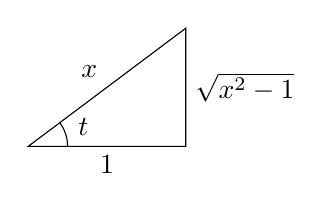
\begin{tikzpicture}
\draw(0,0)--node[below]{$1$}(2,0)--node[right]{$\sqrt{x^{2}-1}$}(2,1.5)--node[above left]{$x$}cycle;
\draw(0.5,0)arc(0:36.869897645844:0.5);
\node at(0.7,0.25){$t$};
\end{tikzpicture}
\end{center}
所以得到
\begin{align*}
-\frac{\ln{\sec{t}}}{\sin{t}}+\ln(\sec{t}+\tan{t})+C=-\frac{x\ln{x}}{\sqrt{x^{2}-1}}+\ln(x+\sqrt{x^{2}-1})+C
\end{align*}\par
{\kaishu 本题更简洁的做法是不用换元, 直接注意到$\frac{\dif{x}}{\sqrt{x^{2}-1}^{3}}=-\dif{\frac{x}{\sqrt{x^{2}-1}}}$即可 (阿贝尔换元的基本操作, 可参考【T4027】) . 但在读者强大到足以注意到这个凑微分的步骤之前, 先用三角换元消根式是更明智的选择. \par
在这里换元$x=\sec{t}$的过程中只需要限制$t\in\left(0,\frac{\pi}{2}\right)$即可, 这是因为$\ln{x}$与$\sqrt{x^{2}-1}$共同限制了这个函数的定义域$x\in\left(1,+\infty\right)$. \par}
{\color{red}【T2025】}$\int x^{2}\sqrt{x+1}\dif{x}$\par
【解】令$\color{blue}x=t^{2}-1,\,t\in\left[0,+\infty\right)$, 则$\color{blue}\sqrt{x+1}=t$, 所以
\begin{align*}
\int x^{2}\sqrt{x+1}\dif{x}={}&\int\qty(t^{2}-1)^{2}t\dif{\qty(t^{2}-1)}\\
={}&2\int\qty(t^{6}-2t^{4}+t^{2})\dif{t}\\
={}&\frac{2}{7}t^{7}-\frac{4}{5}t^{5}+\frac{2}{3}t^{3}+C\\
={}&\frac{2}{7}\sqrt{x+1}^{7}-\frac{4}{5}\sqrt{x+1}^{5}+\frac{2}{3}\sqrt{x+1}^{3}+C
\end{align*}\par
{\kaishu 在处理这类含$\sqrt[n]{ax+b}$的积分时, 可以令$t=\sqrt[n]{ax+b}$, 然后解出$x$关于$t$的函数表达式, 就可以换元实现有理化. \par
另一方面, 这题也可以视为切比雪夫定理的一种情形, 关于切比雪夫定理的内容可以参考附录F.4. \par}
{\color{red}【T2026】}$\int\frac{\dif{x}}{\sqrt{x}+\sqrt[3]{x}}$\par
【解】令$\color{blue}x=t^{6},\,t\in\left(0,+\infty\right)$, 则
\begin{align*}
\int\frac{\dif{x}}{\sqrt{x}+\sqrt[3]{x}}={}&\int\frac{\dif{t^{6}}}{t^{3}+t^{2}}\\
={}&6\int\frac{t^{3}}{t+1}\dif{t}\\
={}&6\int\frac{t^{3}+t^{2}-t^{2}-t+t+1-1}{t+1}\dif{t}\\
={}&6\int\qty(t^{2}-t+1-\frac{1}{t+1})\dif{t}\\
={}&2t^{3}-3t^{2}+6t-6\ln\qty|t+1|+C\\
={}&2\sqrt{x}-3\sqrt[3]{x}+6\sqrt[6]{x}-6\ln\qty|\sqrt[6]{x}+1|+C
\end{align*}\par
{\kaishu 第二类换元法的通常目的是通过换元, 将被积函数变为有理函数或三角 (双曲) 有理函数等形式. 因为这些形式都是可解的, 所以只要能化成这两类积分, 就不用担心无法解题. \par
举例来说, {\color{red}【T2022】}使用三角换元, {\color{red}【T2023】}使用双曲换元, {\color{red}【T2025】}和{\color{red}【T2026】}使用幂函数类型的换元. 在{\color{red}【T2026】}中直接令$x=t^{6}$, 可以一次性消去两个根号, 从而实现有理化. \par}
{\color{red}【T2027】}$\int\frac{1}{2-\sin{x}}\dif{x}$\par
【解】
\begin{align*}
\int\frac{\dif{x}}{2-\sin{x}}={}&\frac{1}{2}\int\frac{\dif{x}}{\cos^{2}{\frac{x}{2}}+\sin^{2}{\frac{x}{2}}-\sin{\frac{x}{2}}\cos{\frac{x}{2}}}\\
={}&\int\frac{\sec^{2}{\frac{x}{2}}}{\sec^{2}{\frac{x}{2}}\qty(\sin^{2}{\frac{x}{2}}-\sin{\frac{x}{2}}\cos{\frac{x}{2}}+\cos^{2}{\frac{x}{2}})}\dif{\frac{x}{2}}\\
={}&\int\frac{\dif{\tan{\frac{x}{2}}}}{\tan^{2}{\frac{x}{2}}-\tan{\frac{x}{2}}+1}\\
={}&\int\frac{\dif{t}}{t^{2}-t+1},\;{\color{blue}t=\tan{\frac{x}{2}}}\\
={}&\int\frac{\dif{\qty(t-\frac{1}{2})}}{\qty(t-\frac{1}{2})^{2}+\qty(\frac{\sqrt{3}}{2})^{2}}\\
={}&\frac{2}{\sqrt{3}}\arctan{\frac{2t-1}{\sqrt{3}}}+C\\
={}&\frac{2}{\sqrt{3}}\arctan{\frac{2\tan{\frac{x}{2}}-1}{\sqrt{3}}}+C
\end{align*}\par
{\color{red}【T2028】}$\int\frac{\dif{x}}{2-\sin{x}}$\par
【解】
\begin{align*}
\int\frac{\dif{x}}{2-\sin{x}}=\int\frac{2+\sin{x}}{4-\sin^{2}{x}}\dif{x}=2\int\frac{\dif{x}}{4-\sin^{2}{x}}+\int\frac{\sin{x}\dif{x}}{4-\sin^{2}{x}}
\end{align*}
分别解这两个积分, 得
\begin{align*}
I_{1}=\int\frac{\dif{x}}{4-\sin^{2}{x}}={}&\int\frac{\sec^{2}{x}\dif{x}}{4\sec^{2}{x}-\tan^{2}{x}}\\
={}&\int\frac{\dif{\tan{x}}}{4+3\tan^{2}{x}}\\
={}&\frac{1}{3}\int\frac{\dif{\tan{x}}}{\tan^{2}{x}+\qty(\frac{2}{\sqrt{3}})^{2}}\\
={}&\frac{1}{2\sqrt{3}}\arctan{\frac{\sqrt{3}\tan{x}}{2}}+C_{1}\\
\\
I_{2}=\int\frac{\sin{x}\dif{x}}{4-\sin^{2}{x}}={}&-\int\frac{\dif{\cos{x}}}{3+\cos^{2}{x}}\\
={}&-\frac{1}{\sqrt{3}}\arctan{\frac{\cos{x}}{\sqrt{3}}}+C_{2}
\end{align*}
所以原积分可表示为
\begin{align*}
2I_{1}+I_{2}=\frac{1}{\sqrt{3}}\arctan{\frac{\sqrt{3}\tan{x}}{2}}-\frac{1}{\sqrt{3}}\arctan{\frac{\cos{x}}{\sqrt{3}}}+C
\end{align*}\par
{\kaishu 这道题目有两种较好的做法, {\color{red}【T2027】}使用万能公式法 (本质是用二倍角公式) , {\color{red}【T2028】}使用平方差分项. 就本题而言, 这两种做法的计算量可以说是不分轩轾. \par
万能公式是通用方法, 能将任何三角有理式积分转化为有理函数积分, 但计算效率较低, 少复杂的被积函数就可能造成非常大的计算量. \par
平方差分项的关键在于, 平方差公式处理后的分母都为二次正余弦函数或常数项, 容易通过恒等式$\sin^{2}{x}+\cos^{2}{x}=1$在三者之间进行转化. 如果分子是常数, 就可以凑$\dif{\tan{x}}$做; 如果分子是一次三角函数, 就凑$\dif{\sin{x}}$或$\dif{\cos{x}}$. 这两种情况在本题中都有所体现. \par}
{\color{red}【T2029】}$\int\frac{\dif{x}}{\sin{x}+2\cos{x}}$\par
【解】
\begin{align*}
\int\frac{\dif{x}}{\sin{x}+2\cos{x}}={}&\int\frac{\dif{x}}{\sqrt{5}\sin(x+\arctan{2})}\\
={}&\frac{1}{\sqrt{5}}\int\csc(x+\arctan{2})\dif{\qty(x+\arctan{2})}\\
={}&\frac{1}{\sqrt{5}}\ln\qty|\tan{\frac{x+\arctan{2}}{2}}|+C
\end{align*}\par
{\color{red}【T2030】}$\int\frac{\dif{x}}{\sin{x}+2\cos{x}}$\par
【解】
\begin{align*}
\int\frac{\dif{x}}{\sin{x}+2\cos{x}}={}&\int\frac{\dif{x}}{2\sin{\frac{x}{2}}\cos{\frac{x}{2}}+2\cos^{2}{\frac{x}{2}}-2\sin^{2}{\frac{x}{2}}}\\
={}&\int\frac{\sec^{2}\frac{x}{2}}{-\tan^{2}{\frac{x}{2}}+\tan{\frac{x}{2}}+1}\dif{\frac{x}{2}}\\
={}&\int\frac{\dif{\tan{\frac{x}{2}}}}{-\tan^{2}{\frac{x}{2}}+\tan{\frac{x}{2}}+1}\\
={}&\int\frac{\dif{t}}{-t^{2}+t+1};\,{\color{blue}t=\tan{\frac{x}{2}}}\\
={}&\int\frac{\dif{t}}{\qty(\frac{\sqrt{5}}{2})^{2}-\qty(t-\frac{1}{2})^{2}}\\
={}&\frac{1}{\sqrt{5}}\int\frac{\dif{t}}{t-\frac{1}{2}+\frac{\sqrt{5}}{2}}-\frac{1}{\sqrt{5}}\int\frac{\dif{t}}{t-\frac{1}{2}-\frac{\sqrt{5}}{2}}\\
={}&\frac{1}{\sqrt{5}}\ln\qty|\frac{t-\frac{1}{2}+\frac{\sqrt{5}}{2}}{t-\frac{1}{2}-\frac{\sqrt{5}}{2}}|+C\\
={}&\frac{1}{\sqrt{5}}\ln\qty|\frac{2\tan{\frac{x}{2}}-1+\sqrt{5}}{2\tan{\frac{x}{2}-1-\sqrt{5}}}|+C
\end{align*}\par
{\color{red}【T2031】}$\int\frac{\dif{x}}{\sin{x}+2\cos{x}}$\par
【解】
\begin{align*}
\int\frac{\dif{x}}{\sin{x}+2\cos{x}}=\int\frac{2\cos{x}-\sin{x}}{4\cos^{2}{x}-\sin^{2}{x}}\dif{x}=2\int\frac{\cos{x}\dif{x}}{4\cos^{2}{x}-\sin^{2}{x}}-\int\frac{\sin{x}\dif{x}}{4\cos^{2}{x}-\sin^{2}{x}}
\end{align*}
分别解这两个积分, 得
\begin{align*}
I_{1}=\int\frac{\cos{x}\dif{x}}{4\cos^{2}{x}-\sin^{2}{x}}={}&\int\frac{\dif{\sin{x}}}{4-5\sin^{2}{x}}\\
={}&\frac{\dif{\sin{x}}}{\qty(2-\sqrt{5}\sin{x})\qty(2+\sqrt{5}\sin{x})}\\
={}&\frac{1}{4}\int\frac{\dif{\sin{x}}}{2-\sqrt{5}\sin{x}}+\frac{1}{4}\int\frac{\dif{\sin{x}}}{2+\sqrt{5}\sin{x}}\\
={}&\frac{1}{4\sqrt{5}}\ln\qty|\frac{2+\sqrt{5}\sin{x}}{2-\sqrt{5}\sin{x}}|+C_{1}\\
\\
I_{2}=\int\frac{\sin{x}\dif{x}}{4\cos^{2}{x}-\sin^{2}{x}}={}&-\int\frac{\dif{\cos{x}}}{5\cos^{2}{x}-1}\\
={}&\int\frac{\dif{\cos{x}}}{\qty(1-\sqrt{5}\cos{x})\qty(1+\sqrt{5}\cos{x})}\\
={}&\frac{1}{2}\int\frac{\dif{\cos{x}}}{1-\sqrt{5}\cos{x}}+\frac{1}{2}\int\frac{\dif{\cos{x}}}{1+\sqrt{5}\cos{x}}\\
={}&\frac{1}{2\sqrt{5}}\ln\qty|\frac{1+\sqrt{5}\cos{x}}{1-\sqrt{5}\cos{x}}|+C_{2}
\end{align*}
所以原积分可表示为
\begin{align*}
2I_{1}-I_{2}=\frac{1}{2\sqrt{5}}\ln\qty|\frac{2+\sqrt{5}\sin{x}}{2-\sqrt{5}\sin{x}}|-\frac{1}{2\sqrt{5}}\ln\qty|\frac{1+\sqrt{5}\cos{x}}{1-\sqrt{5}\cos{x}}|+C
\end{align*}\par
{\kaishu 对于$\int\frac{\dif{x}}{a\sin{x}+b\cos{x}}$类型的问题, 万能公式法和平方差分项也是伯仲之间, 但明显像{\color{red}【T2029】}那样套用辅助角公式会更快. 这题还有另一种做法, 见{\color{red}【T3025】}. \par}
【T2032】$\int\cot^{2}{x}\tan{\frac{1+x\tan{x}}{\tan{x}}}\dif{x}$\par
【解】
\begin{align*}
\int\cot^{2}{x}\tan{\frac{1+x\tan{x}}{\tan{x}}}\dif{x}={}&\int\qty(\csc^{2}{x}-1)\tan(\cot{x}+x)\dif{x}\\
={}&-\int\tan(\cot{x}+x)\dif{\qty(\cot{x}+x)}\\
=\ln\qty|\cos(x+\cot{x})|+C
\end{align*}\par
{\kaishu 这题的难点在于$\tan{\frac{1+x\tan{x}}{\tan{x}}}$. 要处理这个复合函数, 一方面要尽量想办法将其化简, 另一方面应当尽可能从其它部分挖掘出能凑微分成$u=\frac{1+x\tan{x}}{\tan{x}}$的部分. \par}
【T2033】$\int\sqrt{x+2+\sqrt{\qty(x+1)\qty(x+3)}}\dif{x}$\par
【解】
\begin{align*}
{}&\int\sqrt{x+2+\sqrt{\qty(x+1)\qty(x+3)}}\dif{x}\\
={}&\frac{1}{\sqrt{2}}\int\sqrt{2x+4+2\sqrt{\qty(x+1)\qty(x+3)}}\dif{x}\\
={}&\frac{1}{\sqrt{2}}\int\sqrt{\qty(x+1)+\qty(x+3)+2\sqrt{x+1}\sqrt{x+3}}\dif{x}\\
={}&\frac{1}{\sqrt{2}}\int\sqrt{\sqrt{x+1}^{2}+\sqrt{x+3}^{2}+2\sqrt{x+1}\sqrt{x+3}}\dif{x}\\
={}&\frac{1}{\sqrt{2}}\int\sqrt{\qty(\sqrt{x+1}+\sqrt{x+3})^{2}}\dif{x}\\
={}&\frac{1}{\sqrt{2}}\int\qty(\sqrt{x+1}+\sqrt{x+3})\dif{x}\\
={}&\frac{\sqrt{2}}{3}\qty(x+1)^{\frac{3}{2}}+\frac{\sqrt{2}}{3}\qty(x+3)^{\frac{3}{2}}+C
\end{align*}\par
{\kaishu 这里体现了观察被积函数结构的重要性. 倘若不能注意到凑完全平方式的操作, 解题就会变得难以下手. 这就需要读者多积累做题经验. \par
注意一点, 在这里可以求出被积函数的定义域为$\left[-1,+\infty\right)$, 所以$x+1=\sqrt{x+1}^{2},\\\sqrt{\qty(x+1)\qty(x+3)}=\sqrt{x+1}\sqrt{x+3}$等恒等变换式都是成立的. 否则就需要分类讨论等, 以防出错. \par}
【T2034】$\int\frac{\arcsin{x}\arccos{x}}{\sqrt{1-x^{2}}}\dif{x}$\par
【解】
\begin{align*}
\int\frac{\arcsin{x}\arccos{x}}{\sqrt{1-x^{2}}}\dif{x}={}&\int\arcsin{x}\arccos{x}\dif{\arcsin{x}}\\
={}&\int\arcsin{x}\qty(\frac{\pi}{2}-\arcsin{x})\dif{\arcsin{x}}\\
={}&\frac{\pi}{2}\int\arcsin{x}\dif{\arcsin{x}}-\int\arcsin^{2}{x}\dif{\arcsin{x}}\\
={}&\frac{\pi}{4}\arcsin^{2}{x}-\frac{1}{3}\arcsin^{3}{x}+C
\end{align*}\par
{\kaishu 关于反三角函数的常用恒等变换, 读者是有必要了解的. \par}
\chapter*{三级题目}
\addcontentsline{toc}{chapter}{三级题目}
\fancyhead[RE,LO]{\kaishu 三级题目}
{\color{red}【T3001】}$\int\frac{\dif{x}}{ax^{2}+bx+c}\;\left(a>0\right)$\par
【解】当$b^{2}-4ac<0$时, 
\begin{align*}
\int\frac{\dif{x}}{ax^{2}+bx+c}={}&\int\frac{\dif{x}}{\qty(\sqrt{a}x+\frac{b}{2\sqrt{a}})^{2}+c-\frac{b^{2}}{4a}}\\
={}&\frac{1}{\sqrt{a}}\int\frac{\dif{\qty(\sqrt{a}x+\frac{b}{2\sqrt{a}})}}{\qty(\sqrt{a}x+\frac{b}{2\sqrt{a}})^{2}+\frac{4ac-b^{2}}{4a}}\\
={}&\frac{1}{\sqrt{a}}\cdot\frac{2\sqrt{a}}{\sqrt{4ac-b^{2}}}\arctan{\frac{2\sqrt{a}\qty(\sqrt{a}x+\frac{b}{2\sqrt{a}})}{\sqrt{4ac-b^{2}}}}+C_{1}\\
={}&\frac{2}{\sqrt{4ac-b^{2}}}\arctan{\frac{2ax+b}{\sqrt{4ac-b^{2}}}}+C_{1}
\end{align*}
当$b^{2}-4ac=0$时, 
\begin{align*}
\int\frac{\dif{x}}{ax^{2}+bx+c}={}&\frac{1}{\sqrt{a}}\int\frac{\dif{\qty(\sqrt{a}x+\frac{b}{2\sqrt{a}})}}{\qty(\sqrt{a}x+\frac{b}{2\sqrt{a}})^{2}}\\
={}&-\frac{1}{\sqrt{a}}\cdot\frac{1}{\sqrt{a}x+\frac{b}{2\sqrt{a}}}+C_{2}\\
={}&-\frac{2}{2ax+b}+C_{2}
\end{align*}
当$b^{2}-4ac>0$时, 
\begin{align*}
\int\frac{\dif{x}}{ax^{2}+bx+c}={}&\frac{1}{a}\int\frac{\dif{x}}{\qty(x-\frac{-b-\sqrt{b^{2}-4ac}}{2a})\qty(x-\frac{-b+\sqrt{b^{2}-4ac}}{2a})}\\
={}&\frac{1}{\sqrt{b^{2}-4ac}}\qty(\int\frac{\dif{x}}{x+\frac{b-\sqrt{b^{2}-4ac}}{2a}}-\int\frac{\dif{x}}{x+\frac{b+\sqrt{b^{2}-4ac}}{2a}})\\
={}&\frac{1}{\sqrt{b^{2}-4ac}}\ln\qty|\frac{x+\frac{b-\sqrt{b^{2}-4ac}}{2a}}{x+\frac{b+\sqrt{b^{2}-4ac}}{2a}}|+C_{3}\\
={}&\frac{1}{\sqrt{b^{2}-4ac}}\ln\qty|\frac{2ax+b-\sqrt{b^{2}-4ac}}{2ax+b+\sqrt{b^{2}-4ac}}|+C_{3}
\end{align*}
综上所述, 得到
\begin{align*}
\int\frac{\dif{x}}{ax^{2}+bx+c}=\begin{cases}
\frac{2}{\sqrt{4ac-b^{2}}}\arctan{\frac{2ax+b}{\sqrt{4ac-b^{2}}}}+C_{1},&b^{2}-4ac<0\\
-\frac{2}{2ax+b}+C_{2},&b^{2}-4ac=0\\
\frac{1}{\sqrt{b^{2}-4ac}}\ln\qty|\frac{2ax+b-\sqrt{b^{2}-4ac}}{2ax+b+\sqrt{b^{2}-4ac}}|+C_{3},&b^{2}-4ac>0
\end{cases}
\end{align*}\par
{\kaishu 这里呈现的是一个有理函数积分通式. 如果能够记忆, 将有助于加快解题速度. 这种情形非常常见, 并且容易推导通式, 所以三级题目开始不再给出解决这个问题的具体过程. \par}
{\color{red}【T3002】}$\int\frac{2x+1}{\qty(x-1)\qty(x-2)\qty(x+3)}\dif{x}$\par
【解】设$\frac{2x+1}{\qty(x-1)\qty(x-2)\qty(x+3)}=\frac{A}{x-1}+\frac{B}{x-2}+\frac{C}{x+3}$, 用留数法求出
\begin{align*}
A={}&\eval{\frac{2x+1}{\qty(x-2)\qty(x+3)}}_{x-1=0}=-\frac{3}{4}\\
B={}&\eval{\frac{2x+1}{\qty(x-1)\qty(x+3)}}_{x-2=0}=1\\
C={}&\eval{\frac{2x+1}{\qty(x-1)\qty(x-2)}}_{x+3=0}=-\frac{1}{4}
\end{align*}
所以
\begin{align*}
\int\frac{2x+1}{\qty(x-1)\qty(x-2)\qty(x+3)}\dif{x}={}&-\frac{3}{4}\int\frac{\dif{x}}{x-1}+\int\frac{\dif{x}}{x-2}-\frac{1}{4}\int\frac{\dif{x}}{x+3}\\
={}&-\frac{3}{4}\ln\qty|x-1|+\ln\qty|x-2|-\frac{1}{4}\ln\qty|x+3|+C
\end{align*}\par
{\kaishu 这是留数法在有理函数裂项中的应用, 本题是最简单的分母只含一次单因式情形. 概括来说, 要确定一个待定式, 就将相应的分母$x-a$从原因式的分母中消去, 再代入$x-a=0$ (或$x=a$) 将这个式子解出, 就可以求得待定式. \par
关于留数法裂项的推导和详细操作, 可以参考附录C.4. \par}
{\color{red}【T3003】}$\int\frac{1}{x^{2}\qty(x+1)^{2}}\dif{x}$\par
【解】设$\frac{1}{x^{2}\qty(x+1)^{2}}=\frac{A}{x^{2}}+\frac{B}{x}+\frac{D}{\qty(x+1)^{2}}+\frac{E}{x+1}$, 用留数法求出
\begin{align*}
A={}&\eval{\frac{1}{\qty(x+1)^{2}}}_{x=0}=1\\
B={}&\eval{\dv{\frac{1}{\qty(x+1)^{2}}}{x}}_{x=0}=\eval{-\frac{2}{x+1}}_{x=0}=-2\\
D={}&\eval{\frac{1}{x^{2}}}_{x+1=0}=1\\
E={}&\eval{\dv{\frac{1}{x^{2}}}{\qty(x+1)}}_{x+1=0}=\eval{-\frac{2}{x^{3}}}_{x+1=0}=2
\end{align*}
所以
\begin{align*}
\frac{\dif{x}}{x^{2}\qty(x+1)^{2}}\dif{x}={}&\int\frac{\dif{x}}{x^{2}}-2\int\frac{\dif{x}}{x}+\int\frac{\dif{x}}{\qty(x+1)^{2}}+2\int\frac{\dif{x}}{x+1}\\
={}&-\frac{1}{x}-2\ln\qty|x|-\frac{1}{x+1}+2\ln\qty|x+1|+C
\end{align*}\par
{\kaishu 这是留数法在处理分母含一次重因式时的做法. 裂项时设待定式的方式和待定系数法是如出一辙的, 但后续操作有所不同. 如果一个待定式对应的分母$\qty(x-a)^{n}$和原式当中的重数相同, 那么仿照{\color{red}【T3002】}中的方法求未知量即可. 
而如果待定式的分母次数低于原式当中的重数, 那么低$m$次就需要求$m$阶导再代入$x-a=0$, 最后还要记得除$m!$. \par}
{\color{red}【T3004】}$\int\frac{\dif{x}}{x\qty(x^{5}+1)^{3}}$\par
【解】
\begin{align*}
\int\frac{\dif{x}}{x\qty(x^{5}+1)^{3}}\dif{x}=\int\frac{x^{4}\dif{x}}{x^{5}\qty(x^{5}+1)^{3}}=\frac{1}{5}\int\frac{\dif{x^{5}}}{x^{5}\qty(x^{5}+1)^{3}}
\end{align*}
令$\color{blue}u=x^{5}$, 并设$\frac{1}{u\qty(u+1)^{3}}=\frac{A}{u}+\frac{B}{\qty(u+1)^{3}}+\frac{D}{\qty(u+1)^{2}}+\frac{E}{u+1}$, 用留数法求出
\begin{align*}
A={}&\eval{\frac{1}{\qty(u+1)^{3}}}_{u=0}=1\\
B={}&\eval{\frac{1}{u}}_{u+1=0}=-1\\
D={}&\eval{\dv{\frac{1}{u}}{\qty(u+1)}}_{u+1=0}=\eval{-\frac{1}{u^{2}}}_{u+1=0}=-1\\
E={}&\eval{\frac{1}{2}\cdot\dv[2]{\frac{1}{u}}{\qty(u+1)}}_{u+1=0}=\eval{\frac{1}{u^{3}}}_{u+1=0}=-1
\end{align*}
所以
\begin{align*}
\frac{1}{5}\int\frac{\dif{x^{5}}}{x^{5}\qty(x^{5}+1)^{3}}={}&\frac{1}{5}\int\qty[\frac{1}{u}-\frac{1}{\qty(u+1)^{3}}-\frac{1}{\qty(u+1)^{2}}-\frac{1}{u+1}]\dif{u}\\
={}&\frac{1}{5}\int\frac{\dif{u}}{u}-\frac{1}{5}\int\frac{\dif{u}}{u+1}-\frac{1}{5}\int\frac{\dif{u}}{\qty(u+1)^{2}}-\frac{1}{5}\int\frac{\dif{u}}{\qty(u+1)^{3}}\\
={}&\frac{1}{5}\ln\qty|\frac{u}{u+1}|+\frac{1}{5\qty(u+1)}+\frac{1}{10\qty(u+1)^{2}}\\
={}&\frac{1}{5}\ln\qty|\frac{x^{5}}{x^{5}+1}|+\frac{1}{5x^{5}+5}+\frac{1}{10\qty(x^{5}+1)^{2}}+C
\end{align*}\par
{\kaishu 本例中倘若直接对被积函数进行暴力裂项, 将会得到十分复杂的结果. 这时读者切记不能思维固化, 应当寻找适当的方法来简化问题. 本例中使用换元$u=x^{5}$就能将分母变成关于$u$的四次形式, 比原来关于$x$的十六次形式要容易很多. \par
再次提醒, 求$E$的时候要注意带个系数$\frac{1}{2!}$, 这是很容易被遗忘的. 原理参考附录C.4.3. \par}
{\color{red}【T3005】}$\int\frac{\dif{x}}{x^{3}+1}$\par
【解】设$\frac{1}{x^{3}+1}=\frac{A}{x+1}+\frac{B}{x^{2}-x+1}$, 用留数法求出
\begin{align*}
A={}&\eval{\frac{1}{x^{2}-x+1}}_{x+1=0}=\frac{1}{3}\\
\\
B={}&\eval{\frac{1}{x+1}}_{x^{2}-x+1=0}\\
={}&\eval{\frac{x-2}{x^{2}-x-2}}_{x^{2}-x+1=0}\\
={}&\eval{\frac{x-2}{x^{2}-x+1-3}}_{x^{2}-x+1=0}\\
={}&-\frac{x-2}{3}
\end{align*}
所以
\begin{align*}
\int\frac{\dif{x}}{x^{3}+1}={}&\frac{1}{3}\int\frac{\dif{x}}{x+1}-\frac{1}{3}\int\frac{x-2}{x^{2}-x+1}\dif{x}\\
={}&\frac{1}{3}\ln\qty|x+1|-\frac{1}{6}\int\frac{2x-1}{x^{2}-x+1}\dif{x}+\frac{1}{2}\int\frac{\dif{x}}{x^{2}-x+1}\\
={}&\frac{1}{3}\ln\qty|x+1|-\frac{1}{6}\ln\qty(x^{2}-x+1)+\frac{1}{\sqrt{3}}\arctan{\frac{2x-1}{\sqrt{3}}}+C
\end{align*}\par
{\kaishu 这是留数法在处理分母含二次单因式时的做法. 这里所设的$B$是一个待定 (一次) 多项式, 而不是待定的常数. 以本题为例, 做题者只需要将$\frac{1}{x+1}$化成一次多项式形式即可, 而条件是$x^{2}-x+1=0$. \par
鉴于分母的多项式很难消除, 这里考虑在分子分母同乘其它多项式, 以便在分母上凑出含$x^{2}-x$的形式, 再用$-1$代换之. \par}
{\color{red}【T3006】}$\int\frac{\dif{x}}{x^{3}-1}$\par
【解】设$\frac{1}{x^{3}-1}=\frac{A}{x-1}+\frac{B}{x^{2}+x+1}$, 用模法求出
\begin{align*}
A={}&\frac{1}{x^{2}+x+1}\m\qty(x-1)=\frac{1}{3}\\
\\
B={}&\frac{1}{x-1}\m\qty(x^{2}+x+1)\\
={}&\frac{x+2}{x^{2}+x-2}\m\qty(x^{2}+x+1)\\
={}&\frac{x+2}{x^{2}+x+1-3}\m\qty(x^{2}+x+1)\\
={}&-\frac{x+2}{3}
\end{align*}
所以
\begin{align*}
\int\frac{\dif{x}}{x^{3}-1}={}&\frac{1}{3}\int\frac{\dif{x}}{x-1}-\frac{1}{3}\int\frac{x+2}{x^{2}+x+1}\dif{x}\\
={}&\frac{1}{3}\ln\qty|x-1|-\frac{1}{6}\int\frac{2x+1}{x^{2}+x+1}\dif{x}-\frac{1}{2}\int\frac{\dif{x}}{x^{2}+x+1}\\
={}&\frac{1}{3}\ln\qty|x-1|-\frac{1}{6}\ln(x^{2}+x+1)-\frac{1}{\sqrt{3}}\arctan{\frac{2x+1}{\sqrt{3}}}+C
\end{align*}\par
{\kaishu 这是模法在有理函数裂项中的应用. 对于分母只含单因式的情形, 模法与留数法的操作除了写法以外别无二致. 然而在处理分母含重因式的情形时, 两种方法则可以说是各有千秋. 关于模法的相关介绍, 可以参考附录C.5. \par}
【T3007】$\int\frac{x^{2}}{x^{4}-x^{2}+1}\dif{x}$\par
【解】考虑到
\begin{align*}
x^{4}+x^{2}+1=\qty(x^{2}+1)^{2}-x^{2}=\qty(x^{2}-x+1)\qty(x^{2}+x+1)
\end{align*}
设$\frac{x^{2}}{x^{4}+x^{2}+1}=\frac{A}{x^{2}-x+1}+\frac{B}{x^{2}+x+1}$, 用模法求出
\begin{align*}
A={}&\frac{x^{2}}{x^{2}+x+1}\m\qty(x^{2}-x+1)\\
={}&\frac{x^{2}}{\qty(x^{2}-x+1)+2x}\m\qty(x^{2}-x+1)\\
={}&\frac{x^{2}}{2x}\m\qty(x^{2}-x+1)\\
={}&\frac{x}{2}\\
\\
B={}&\frac{x^{2}}{x^{2}-x+1}\m\qty(x^{2}+x+1)\\
={}&\frac{x^{2}}{\qty(x^{2}+x+1)-2x}\m\qty(x^{2}+x+1)\\
={}&\frac{x^{2}}{-2x}\m\qty(x^{2}+x+1)\\
={}&-\frac{x}{2}
\end{align*}
所以
\begin{align*}
{}&\int\frac{x^{2}}{x^{4}+x^{2}+1}\dif{x}\\
={}&\frac{1}{2}\int\frac{x}{x^{2}-x+1}\dif{x}-\frac{1}{2}\int\frac{x}{x^{2}+x+1}\dif{x}\\
={}&\frac{1}{4}\int\frac{2x-1}{x^{2}-x+1}\dif{x}+\frac{1}{4}\int\frac{\dif{x}}{x^{2}-x+1}-\frac{1}{4}\int\frac{2x+1}{x^{2}+x+1}\dif{x}+\frac{1}{4}\int\frac{\dif{x}}{x^{2}+x+1}\\
={}&\frac{1}{4}\ln{\frac{x^{2}-x+1}{x^{2}+x+1}}+\frac{1}{2\sqrt{3}}\arctan{\frac{2x-1}{\sqrt{3}}}+\frac{1}{2\sqrt{3}}\arctan{\frac{2x+1}{\sqrt{3}}}+C
\end{align*}\par
{\kaishu 关于$x^{4}+kx^{2}+1\;\qty(k\le2)$的因式分解, 可以仿照本题中的平方差思路进行. \par}
【T3008】$\int\frac{x-2}{x^{4}+2x^{3}-3x^{2}-4x+4}\dif{x}$\par
【解】考虑到
\begin{align*}
x^{4}+2x^{3}-3x^{2}-4x+4=\qty(x-1)^{2}\qty(x+2)^{2}
\end{align*}
设$\frac{x-2}{x^{4}+2x^{3}-3x^{2}-4x+4}=\frac{A}{\qty(x-1)^{2}}+\frac{B}{\qty(x+2)^{2}}$, 用模法求出
\begin{align*}
A={}&\frac{x-2}{\qty(x+2)^{2}}\m\qty(x-1)^{2}\\
={}&\frac{x-2}{x^{2}-2x+1+6x+3}\m\qty(x^{2}-2x+1)\\
={}&\frac{1}{3}\cdot\frac{\qty(x-2)\qty(x-\frac{5}{2})}{\qty(2x+1)\qty(x-\frac{5}{2})}\m\qty(x^{2}-2x+1)\\
={}&\frac{1}{3}\cdot\frac{x^{2}-\frac{9}{2}x+5}{2x^{2}-4x-\frac{5}{2}}\m\qty(x^{2}-2x+1)\\
={}&\frac{1}{3}\cdot\frac{-\frac{5}{2}x+4}{-\frac{9}{2}}\\
={}&\frac{5x-8}{27}\\
\\
B={}&\frac{x-2}{\qty(x-1)^{2}}\m\qty(x+2)^{2}\\
={}&\frac{x-2}{x^{2}+4x+4-6x-3}\m\qty(x^{2}+4x+4)\\
={}&-\frac{1}{3}\cdot\frac{\qty(x-2)\qty(x+\frac{7}{2})}{\qty(2x+1)\qty(x+\frac{7}{2})}\m\qty(x^{2}+4x+4)\\
={}&-\frac{1}{3}\cdot\frac{x^{2}+\frac{3}{2}x-7}{2x^{2}+8x+\frac{7}{2}}\m\qty(x^{2}+4x+4)\\
={}&-\frac{1}{3}\cdot\frac{-\frac{5}{2}x-11}{\frac{27}{2}}\\
={}&-\frac{5x+22}{27}
\end{align*}
所以
\begin{align*}
\int\frac{x-2}{x^{4}+2x^{3}-3x^{2}-4x+4}\dif{x}={}&\frac{1}{27}\int\frac{5x-8}{\qty(x-1)^{2}}\dif{x}-\frac{1}{27}\int\frac{5x+22}{\qty(x+2)^{2}}\dif{x}\\
={}&\frac{5}{27}\int\frac{\dif{x}}{x-1}-\frac{1}{9}\int\frac{\dif{x}}{\qty(x-1)^{2}}-\frac{5}{27}\int\frac{\dif{x}}{x+2}-\frac{4}{9}\int\frac{\dif{x}}{\qty(x+2)^{2}}\\
={}&\frac{5}{27}\ln\qty|\frac{x-1}{x+2}|+\frac{1}{9\qty(x-1)}+\frac{4}{9\qty(x+2)}+C
\end{align*}\par
{\kaishu 本题涉及到分母含重因式时的模法应用. 与留数法不同, 模法要求只将分母中不同的因子分离开, 而重因式不再需要进一步分离. 这里设出的$A,\,B$都是比分母低一次的待定多项式. \par
另外, 这里还涉及高次多项式因式分解的一个套路, 就是试根. 对于整系数多项式 (如本题) , 可以将常数项的因数 (如本题的$\pm1,\,\pm2,\,\pm4$) 代入计算多项式的值. 如果得到$0$, 则这个数是多项式的一个根. 于是可以先将这个根对应的因式先分解出来, 再按此法处理剩下的部分, 直到因式分解完毕. \par}
{\color{red}【T3009】}$\int\frac{3x^{2}+1}{x^{4}+1}\dif{x}$\par
【解】
\begin{align*}
\int\frac{3x^{2}+1}{x^{4}+1}\dif{x}=2\int\frac{x^{2}+1}{x^{4}+1}\dif{x}+\int\frac{x^{2}-1}{x^{4}+1}\dif{x}
\end{align*}
分别解这两个积分, 得
\begin{align*}
I_{1}=\int\frac{x^{2}+1}{x^{4}+1}\dif{x}={}&\int\frac{1+x^{-2}}{x^{2}+x^{-2}}\dif{x}\\
={}&\int\frac{\dif{\qty(x-x^{-1})}}{\qty(x-x^{-1})^{2}+2}\\
={}&\frac{1}{\sqrt{2}}\arctan{\frac{x-x^{-1}}{\sqrt{2}}}+C_{1}\\
\\
I_{2}=\int\frac{x^{2}-1}{x^{4}+1}\dif{x}={}&\int\frac{1-x^{-2}}{x^{2}+x^{-2}}\dif{x}\\
={}&\int\frac{\dif{\qty(x+x^{-1})}}{\qty(x+x^{-1})^{2}-2}\\
={}&\frac{1}{2\sqrt{2}}\ln\qty|\frac{x+x^{-1}-\sqrt{2}}{x+x^{-1}+\sqrt{2}}|+C_{2}
\end{align*}
所以原积分可化为
\begin{align*}
2I_{1}+I_{2}=\sqrt{2}\arctan{\frac{x-x^{-1}}{\sqrt{2}}}+\frac{1}{2\sqrt{2}}\ln\qty|\frac{x+x^{-1}-\sqrt{2}}{x+x^{-1}+\sqrt{2}}|+C
\end{align*}\par
{\kaishu 本题涉及到$\int\frac{x^{2}\pm1}{x^{4}+1}\dif{x}$的积分问题. 这两个积分是可以通过裂项来解决的, 分母因式分解的等式为$x^{4}+1=\qty(x^{2}-\sqrt{2}x+1)\qty(x^{2}+\sqrt{2}x+1)$. 不过, 倘若分子分母同除$x^{2}$凑对勾换元, 就像本题中的$I_{1}$和$I_{2}$那样, 解题就会相当快捷. \par
本题还涉及积木法的使用. 如果一言以蔽之的话, 积木法就是将难以解决的积分通过适当的分项转化成若干个容易解决的积分, 从而解决原积分的过程. 比如说, $\int\frac{ax^{2}+b}{x^{4}+1}\dif{x}$是难以解决的积分, 而$\int\frac{x^{2}+1}{x^{4}+1}\dif{x}$和$\int\frac{x^{2}-1}{x^{4}+1}\dif{x}$是解决起来相对容易的. 于是我们只要解出后者就能够将前者表示出来. 前面所讲的分项积分都可以认为是积木法, 类似的更复杂问题还有【T5001】. \par}
{\color{red}【T3010】}$\int\frac{1}{\sqrt{x\qty(x+1)}}\dif{x}$\par
【解】当$x>0$时, 
\begin{align*}
\int\frac{\dif{x}}{\sqrt{x\qty(x+1)}}={}&\int\frac{\dif{x}}{\sqrt{x}\sqrt{x+1}}=2\int\frac{\dif{\sqrt{x}}}{\sqrt{\sqrt{x}^{2}+1}}=2\ln(\sqrt{x}+\sqrt{x+1})+C
\end{align*}
当$x<-1$时, 
\begin{align*}
\int\frac{\dif{x}}{\sqrt{x\qty(x+1)}}={}&\int\frac{\dif{x}}{\sqrt{-x}\sqrt{-x-1}}
=-2\int\frac{\dif{\sqrt{-x}}}{\sqrt{\sqrt{-x}^{2}-1}}
=-2\ln(\sqrt{-x}+\sqrt{-x-1})+C
\end{align*}
综上所述, 得到
\begin{align*}
\int\frac{\dif{x}}{\sqrt{x\qty(x+1)}}=\begin{cases}
2\ln(\sqrt{x}+\sqrt{x+1})+C_{1},&x>0\\
-2\ln(\sqrt{-x}+\sqrt{-x-1})+C_{2},&x<-1
\end{cases}
\end{align*}\par
{\kaishu 这种方法能避开配方$\int\frac{\dif{x}}{\sqrt{\qty(x+\frac{1}{2})^{2}-\frac{1}{4}}}$再求解的过程, 但需要注意拆根式时考虑$x$的取值范围, 否则容易产生错解. \par}
{\color{red}【T3011】}$\int x^{5}\sqrt{x^{3}+1}\dif{x}$\par
【解】
\begin{align*}
\int x^{5}\sqrt{x^{3}+1}\dif{x}=\frac{1}{3}\int x^{3}\sqrt{x^{3}+1}\dif{x^{3}}
\end{align*}
令$\color{blue}x^{3}=t^{2}-1,\,t\in\left[0,+\infty\right)$, 则$\color{blue}t=\sqrt{x^{3}+1}$, 所以
\begin{align*}
\frac{1}{3}\int x^{3}\sqrt{x^{3}+1}\dif{x^{3}}={}&\frac{1}{3}\int\qty(t^{2}-1)t\dif{t^{2}}\\
={}&\frac{2}{3}\int\qty(t^{4}-t^{2})\dif{t}\\
={}&\frac{2}{15}t^{5}-\frac{2}{9}t^{3}+C\\
={}&\frac{2}{15}\sqrt{x^{3}+1}^{5}-\frac{2}{9}\sqrt{x^{3}+1}^{3}+C
\end{align*}\par
{\kaishu 这是切比雪夫定理在处理无理函数积分时的应用. 这里要解决的主要问题是$\sqrt{x^{3}+1}$, 为了简化计算, 可以考虑整体换元$u=x^{3}$再进一步操作, 这就需要适当凑微分. 这里将$u=x^{3}$与接下来消根式的换元$u=t^{2}-1$合并为一步, 读者在熟练掌握切比雪夫定理后应当熟悉这样的操作. \par
有关切比雪夫定理的内容, 可见附录F.4. \par}
{\color{red}【T3012】}$\int\sqrt{\frac{x}{x+1}}\dif{x}$\par
【解】令$\color{blue}t=\sqrt{\frac{x}{x+1}},\,t\in\left[0,1\right)\cup\left(1,+\infty\right)$, 则$\color{blue}x=\frac{t^{2}}{1-t^{2}}$, 所以
\begin{align*}
\int\sqrt{\frac{x}{x+1}}\dif{x}={}&\int t\dif{\frac{t^{2}}{1-t^{2}}}\\
={}&\int t\dif{\qty(\frac{1}{1-t^{2}}-1)}\\
={}&\int t\dif{\frac{1}{1-t^{2}}}\\
={}&\frac{t}{1-t^{2}}-\int\frac{\dif{t}}{1-t^{2}}\\
={}&\frac{t}{1-t^{2}}+\frac{1}{2}\ln\qty|\frac{t-1}{t+1}|+C\\
={}&\qty(x+1)\sqrt{\frac{x}{x+1}}+\frac{1}{2}\ln\qty|\frac{\sqrt{\frac{x}{x+1}}-1}{\sqrt{\frac{x}{x+1}}+1}|+C
\end{align*}\par
{\kaishu 这是分式线性替换在切比雪夫定理中的应用. 当换元将原积分化为$\int t\dif{\frac{t^{2}}{1-t^{2}}}$后, 不要思维惯性只知道求导变成$-2\int\frac{t^{2}\dif{t}}{\qty(t^{2}-1)^{2}}$. 这里显然是分部积分之后再做会更轻松. \par
这里还需要注意, 结果中的$\qty|\frac{\sqrt{\frac{x}{x+1}}-1}{\sqrt{\frac{x}{x+1}}+1}|$不可以画蛇添足地化简为$\qty|\frac{\sqrt{x}-\sqrt{x+1}}{\sqrt{x}+\sqrt{x+1}}|$. 这是因为, 在这个过程中出现了拆根式$\sqrt{\frac{x}{x+1}}=\frac{\sqrt{x}}{\sqrt{x+1}}$的操作, 而这需要一个取值范围$x\in\left[0,+\infty\right)$作为前提. 但是, 实际上被积函数的定义域是$\left(-\infty,-1\right)\cup\left[0,+\infty\right)$, 并不满足拆根式的要求, 会产生错解. \par
同理, $\qty(x+1)\sqrt{\frac{x}{x+1}}$也不能直接化简为$\sqrt{x\qty(x+1)}$. 正确的操作是$\qty(x+1)\sqrt{\frac{x}{x+1}}=\qty(x+1)\frac{\sqrt{x\qty(x+1)}}{\qty|x+1|}=\sgn(x+1)\sqrt{x\qty(x+1)}$. 一般来说, 为了不让式子显得太过臃肿, 只需要保留$\qty(x+1)\sqrt{\frac{x}{x+1}}$就足矣了. \par}
{\color{red}【T3013】}$\int\sqrt{x\qty(x+1)}\dif{x}$\par
【解】令$\color{blue}t=\sqrt{\frac{x}{x+1}},\,t\in\left[0,1\right)\cup\left(1,+\infty\right)$, 则$\color{blue}x=\frac{t^{2}}{1-t^{2}}$, 所以
\begin{align*}
\int\sqrt{x\qty(x+1)}\dif{x}={}&\int\sqrt{\frac{t^{2}}{1-t^{2}}\cdot\frac{1}{1-t^{2}}}\dif{\frac{t^{2}}{1-t^{2}}}\\
={}&\int\sqrt{\frac{t^{2}}{\qty(1-t^{2})^{2}}}\dif{\qty(\frac{t^{2}}{1-t^{2}}-1)}\\
={}&\int\frac{t}{\qty|1-t^{2}|}\dif{\frac{1}{1-t^{2}}}\\
={}&\sgn{\qty(1-t^{2})}\int\frac{t}{1-t^{2}}\dif{\frac{1}{1-t^{2}}}\\
={}&\frac{1}{2}\sgn{\qty(1-t^{2})}\int t\dif{\frac{1}{\qty(1-t^{2})^{2}}}\\
={}&\frac{t\sgn{\qty(1-t^{2})}}{2\qty(1-t^{2})^{2}}-\frac{1}{2}\sgn{\qty(1-t^{2})}\int\frac{\dif{t}}{\qty(t^{2}-1)^{2}}
\end{align*}
接下来解$\int\frac{\dif{t}}{\qty(t^{2}-1)^{2}}$: 
\begin{align*}
\int\frac{\dif{t}}{\qty(t^{2}-1)^{2}}={}&\frac{1}{4}\int\qty(\frac{1}{t-1}-\frac{1}{t+1})^{2}\dif{t}\\
={}&\frac{1}{4}\int\frac{\dif{t}}{\qty(t-1)^{2}}-\frac{1}{2}\int\frac{\dif{t}}{t^{2}-1}+\frac{1}{4}\int\frac{\dif{t}}{\qty(t+1)^{2}}\\
={}&-\frac{1}{4t-4}-\frac{1}{4}\ln\qty|\frac{t-1}{t+1}|-\frac{1}{4t+4}+C_{1}
\end{align*}
所以
\begin{align*}
{}&\int\sqrt{x\qty(x+1)}\dif{x}\\
={}&\frac{t}{2\qty(1-t^{2})\qty|1-t^{2}|}+\frac{1}{2}\qty[\frac{1}{4t-4}+\frac{1}{4t+4}+\frac{1}{4}\ln\qty|\frac{t-1}{t+1}|]\sgn{\qty(1-t^{2})}+C\\
={}&\frac{t}{2\qty(1-t^{2})\qty|1-t^{2}|}-\frac{t}{4\qty|1-t^{2}|}+\frac{1}{8}\ln\qty|\frac{t-1}{t+1}|\sgn{\qty(1-t^{2})}+C\\
={}&\frac{\qty(2x+1)}{4}\sqrt{x\qty(x+1)}+\frac{1}{8}\ln\qty|\frac{\sqrt{\frac{x}{x+1}}-1}{\sqrt{\frac{x}{x+1}}+1}|\sgn{\qty(x+1)}+C
\end{align*}\par
{\kaishu 这是切比雪夫定理一个应用. 在这里依然要注意开偶次根式的诸多问题. 另外, 对于积分$\int\frac{\dif{t}}{\qty(t^{2}-1)^{2}}$, 这里的做法是先在括号内进行裂项, 把被积函数变成$\frac{1}{4}\qty(\frac{1}{t-1}-\frac{1}{t+1})^{2}$, 再进行二项式展开和后续操作, 也是一种不错的方法. \par
本题也是二次根式积分问题, 还可以用三角换元做, 或者仿照{\color{red}【T3022】}的解法来做. \par}
{\color{red}【T3014】}$\int\frac{\dif{x}}{\sqrt[3]{x^{3}+1}}$\par
【解】
\begin{align*}
\int\frac{\dif{x}}{\sqrt[3]{x^{3}+1}}=\frac{1}{3}\int\frac{x^{2}\dif{x}}{x^{2}\sqrt[3]{x^{3}+1}}=\frac{1}{3}\int\frac{\dif{x^{3}}}{x^{2}\sqrt[3]{x^{3}+1}}
\end{align*}
令$\color{blue}t=\sqrt[3]{\frac{x^{3}+1}{x^{3}}}$, 则$\color{blue}x^{3}=\frac{1}{t^{3}-1}$, 所以
\begin{align*}
\frac{1}{3}\int\frac{\dif{x^{3}}}{x^{2}\sqrt[3]{x^{3}+1}}=\frac{1}{3}\int\frac{\dif{\frac{1}{t^{3}-1}}}{\sqrt[3]{\qty(\frac{1}{t^{3}-1})^{2}\cdot\frac{t^{3}}{t^{3}-1}}}=\frac{1}{3}\int\frac{\dif{\frac{1}{t^{3}-1}}}{\frac{t}{t^{3}-1}}=\int\frac{-t\dif{t}}{t^{3}-1}
\end{align*}
设$\frac{-t}{t^{3}-1}=\frac{A}{t-1}+\frac{B}{t^{2}+t+1}$, 用留数法求出
\begin{align*}
A={}&\eval{\frac{-t}{t^{2}+t+1}}_{t-1=0}=-\frac{1}{3}\\
B={}&\eval{\frac{-t}{t-1}}_{t^{2}+t+1=0}=-\eval{\frac{t\qty(t+2)}{t^{2}+t-2}}_{t^{2}+t+1=0}=\frac{t-1}{3}
\end{align*}
所以
\begin{align*}
{}&\int\frac{-t\dif{t}}{t^{3}-1}\\
={}&-\frac{1}{3}\int\frac{\dif{t}}{t-1}+\frac{1}{3}\int\frac{t-1}{t^{2}+t+1}\dif{t}\\
={}&-\frac{1}{3}\ln\qty|t-1|+\frac{1}{6}\int\frac{2t+1}{t^{2}+t+1}\dif{t}-\frac{1}{2}\int\frac{\dif{t}}{t^{2}+t+1}\\
={}&-\frac{1}{3}\ln\qty|t-1|+\frac{1}{6}\ln(t^{2}+t+1)-\frac{1}{\sqrt{3}}\arctan{\frac{2t+1}{\sqrt{3}}}+C\\
={}&-\frac{1}{3}\ln\qty|\sqrt[3]{\frac{x^{3}+1}{x^{3}}}-1|+\frac{1}{6}\ln(\sqrt[3]{\frac{x^{3}+1}{x^{3}}}^{2}+\sqrt[3]{\frac{x^{3}+1}{x^{3}}}+1)-\frac{1}{\sqrt{3}}\arctan{\frac{2\sqrt[3]{x^{3}+1}+x}{\sqrt{3}x}}+C\\
={}&-\frac{1}{3}\ln\qty|\frac{\sqrt[3]{x^{3}+1}-x}{x}|+\frac{1}{6}\ln{\frac{\sqrt[3]{x^{3}+1}^{2}+x\sqrt[3]{x^{3}+1}+x^{2}}{x^{2}}}-\frac{1}{\sqrt{3}}\arctan{\frac{2\sqrt[3]{x^{3}+1}+x}{\sqrt{3}x}}+C
\end{align*}\par
{\kaishu 这里用到了类似于$\sqrt[3]{\frac{x^{3}+1}{x^{3}}}=\frac{\sqrt[3]{x^{3}+1}}{x}$的操作, 这是无可非议的, 因为这里的根式是奇数次的, 开根式无需考虑定义域问题. \par}
【T3015】$\int\frac{x}{\sqrt{1+\sqrt[3]{x^{2}}}}\dif{x}$\par
【解】
\begin{align*}
\int\frac{x}{\sqrt{1+\sqrt[3]{x^{2}}}}\dif{x}={}&\frac{1}{2}\int\frac{\dif{x^{2}}}{\sqrt{1+\sqrt[3]{x^{2}}}}\\
={}&\frac{1}{2}\int\frac{\dif{t^{3}}}{\sqrt{t+1}};\,{\color{blue}t=\sqrt[3]{x^{2}}\in\left[0,+\infty\right)}\\
={}&\frac{3}{2}\int\frac{t^{2}\dif{t}}{\sqrt{t+1}}\\
={}&3\int\qty[\qty(\sqrt{t+1})^{2}-1]^{2}\dif{\sqrt{t+1}}\\
={}&\frac{3}{5}\sqrt{t+1}^{5}-2\sqrt{t+1}^{3}+3\sqrt{t+1}+C\\
={}&\frac{3}{5}\sqrt{\sqrt[3]{x^{2}}+1}^{5}-2\sqrt{\sqrt[3]{x^{2}}+1}^{3}+3\sqrt{\sqrt[3]{x^{2}}+1}+C
\end{align*}\par
{\kaishu 本题看上去有点吓人, 但只要敢做就会发现题目并不难. 本题的标准解答是使用切比雪夫定理, 也就是再令$t=u^{2}-1,\,u\in\left[0,+\infty\right)$, 完全转化成有理函数积分, 但显得太麻烦了, 不如直接凑微分来得痛快. \par}
{\color{red}【T3016】}$\int\frac{1}{\sqrt{\tan{x}}}\dif{x}$\par
【解】
\begin{align*}
\int\frac{\dif{x}}{\sqrt{\tan{x}}}={}&\int\frac{\dif{\tan{x}}}{\qty(\tan^{2}{x}+1)\sqrt{\tan{x}}}\\
={}&\int\frac{\dif{u^{2}}}{u\qty(u^{4}+1)},\;{\color{blue}u=\sqrt{\tan{x}}}\\
={}&2\int\frac{\dif{u}}{u^{4}+1}\\
={}&\int\frac{u^{2}+1}{u^{4}+1}\dif{u}-\int\frac{u^{2}-1}{u^{4}+1}\dif{u}\\
={}&\int\frac{\dif{\qty(u-u^{-1})}}{\qty(u-u^{-1})^{2}+2}-\int\frac{\dif{\qty(u+u^{-1})}}{\qty(u+u^{-1})^{2}-2}\\
={}&\frac{1}{\sqrt{2}}\arctan{\frac{u-u^{-1}}{\sqrt{2}}}-\frac{1}{2\sqrt{2}}\ln\qty|\frac{u+u^{-1}-\sqrt{2}}{u+u^{-1}+\sqrt{2}}|+C\\
={}&\frac{1}{\sqrt{2}}\arctan{\frac{\sqrt{\tan{x}}-\sqrt{\cot{x}}}{\sqrt{2}}}-\frac{1}{2\sqrt{2}}\ln\qty|\frac{\sqrt{\tan{x}}+\sqrt{\cot{x}}-\sqrt{2}}{\sqrt{\tan{x}}-\sqrt{\cot{x}}+\sqrt{2}}|+C
\end{align*}\par
{\kaishu 潜在规律: 如果被积函数是关于$\tan{x}$的有理函数 (或某些特定的无理函数) , 那么直接凑微分$\dif{\tan{x}}$即可解决问题. \par}
{\color{red}【T3017】}$\int\frac{\dif{x}}{x\sqrt{x^{2}+1}}$\par
【解】
\begin{align*}
\int\frac{\dif{x}}{x\sqrt{x^{2}+1}}={}&\int\frac{\dif{x}}{x\qty|x|\sqrt{1+x^{-2}}}\\
={}&\sgn{x}\int\frac{\dif{x}}{x^{2}\sqrt{x^{-2}+1}}\\
={}&-\sgn{x}\int\frac{\dif{x^{-1}}}{\sqrt{x^{-2}+1}}\\
={}&-\ln(x^{-1}+\sqrt{x^{-2}+1})\sgn{x}+C\\
={}&-\ln(\frac{1}{x}+\sqrt{1+\frac{1}{x^{2}}})\sgn{x}+C
\end{align*}\par
{\kaishu 本题是倒代换思路的一种体现, 通过倒代换的方式将原问题转化成{\color{red}【T2022】}一类的已知问题. 这里需要十分注意, 从二次根式中提取因式时应带带绝对值符号, 否则将产生错解. \par
本题的结果式还可以继续化简. 当$x>0$时有$-\ln(\frac{1}{x}+\sqrt{1+\frac{1}{x^{2}}})=\ln{\frac{x}{1+\sqrt{x^{2}+1}}}\\=\ln{\frac{\sqrt{x^{2}+1}-1}{x}}$; 当$x<0$时有$\ln(\frac{1}{x}+\sqrt{1+\frac{1}{x^{2}}})=\ln{\frac{1-\sqrt{x^{2}+1}}{x}}=\ln{\frac{\sqrt{x^{2}+1}-1}{-x}}$. \par
整理一下可以得到更简洁的结果: $\int\frac{\dif{x}}{x\sqrt{x^{2}+1}}=\ln{\frac{\sqrt{x^{2}+1}-1}{\qty|x|}}+C$. \par}
{\color{red}【T3018】}$\int\frac{\dif{x}}{x^{2}\sqrt{x^{2}-1}}$\par
【解】
\begin{align*}
\int\frac{\dif{x}}{x^{2}\sqrt{x^{2}-1}}={}&\int\frac{\dif{x}}{x^{2}\qty|x|\sqrt{1-x^{-2}}}\\
={}&\sgn{x}\int\frac{\dif{x}}{x^{3}\sqrt{1-x^{-2}}}\\
={}&-\frac{1}{2}\sgn{x}\int\frac{\dif{x^{-2}}}{\sqrt{1-x^{-2}}}\\
={}&\sqrt{1-x^{-2}}\sgn{x}+C\\
={}&\frac{\sqrt{x^{2}-1}}{x}+C
\end{align*}\par
{\kaishu 本题的思路和{\color{red}【T3017】}是相似的, 都是旨在通过凑微分的方法向熟知的积分靠拢, 以期避开三角/双曲换元法来解决问题. \par
事实上, 解决这类二次根式积分时笔者不再建议使用三角/双曲换元了. 读者可以只依靠已有的二次根式积分公式 (可以参考【T4001】) 和熟练的恒等变换、凑微分技巧来解决问题, 比如这两道题的做法. 不使用那些换元的原因在于, 解题过程中常常出现因参数取值范围问题导致的错解. 举例来说, $\sqrt{1-x}$要消根号, 就不能用换元$x=\sin{t}$再套二倍角公式, 因为无论如何规定$t$的取值范围, $x$的值域都只能在$\left[-1,1\right]$之内, 而无法涵盖$x\in\left(-\infty,-1\right)$的部分. \par}
{\color{red}【T3019】}$\int\frac{\dif{x}}{\sqrt{\e^{2x}+\e^{x}+1}}$\par
【解】
\begin{align*}
\int\frac{\dif{x}}{\sqrt{\e^{2x}+\e^{x}+1}}={}&\int\frac{\e^{-x}\dif{x}}{\sqrt{1+\e^{-x}+\e^{-2x}}}\\
={}&-\int\frac{\dif{\e^{-x}}}{\sqrt{\e^{-2x}+\e^{-x}+1}}\\
={}&-\int\frac{\dif{u}}{\sqrt{u^{2}+u+1}};\,{\color{blue}u=\e^{-x}}\\
={}&-\int\frac{\dif{\qty(u+\frac{1}{2})}}{\sqrt{\qty(u+\frac{1}{2})^{2}+\qty(\frac{\sqrt{3}}{2})^{2}}}\\
={}&-\int\frac{\dif{\qty(\frac{2u+1}{\sqrt{3}})}}{\sqrt{\qty(\frac{2u+1}{\sqrt{3}})^{2}+1}}\\
={}&-\ln(\frac{2u+1}{\sqrt{3}}+\sqrt{\frac{4u^{2}+4u+4}{3}})+C\\
={}&-\ln(2\e^{-x}+1+2\sqrt{\e^{-2x}+\e^{-x}+1})+C
\end{align*}\par
{\kaishu 正常的有理化思路都是凑$\dif{\e^{x}}$换元消掉指数函数, 将原积分变为常见的无理函数积分来处理. 但是有些时候通过被积函数的结构可以发现凑$\dif{\e^{-x}}$将是更简单的选择. 这一点可以通过相应无理函数的处理方式来理解, 毕竟化为$\int\frac{\dif{t}}{t\sqrt{t^{2}+t+1}}\;\qty(t=\e^{x})$之后也是倒代换解决起来更方便, 那么还不如一开始就令$u=\e^{-x}$, 相当于把倒代换操作一并完成了. \par}
【T3020】$\int\frac{1}{\qty(x+2)\sqrt{x^{2}+1}}\dif{x}$\par
【解】令$\color{blue}t=\frac{1}{x+2}$, 则$\color{blue}x=\frac{1}{t}-2$, 所以
\begin{align*}
{}&\int\frac{\dif{x}}{\qty(x+2)\sqrt{x^{2}+1}}\\
={}&\int\frac{t}{\sqrt{\frac{1}{t^{2}}-\frac{4}{t}+5}}\dif{\frac{1}{t}}\\
={}&-\sgn{t}\int\frac{\dif{t}}{\sqrt{5t^{2}-4t+1}}\dif{t}\\
={}&-\frac{1}{\sqrt{5}}\sgn{t}\int\frac{\dif{\qty(\sqrt{5}t-\frac{2}{\sqrt{5}})}}{\sqrt{\qty(\sqrt{5}t-\frac{2}{\sqrt{5}})^{2}+\qty(\frac{1}{\sqrt{5}})^{2}}}\\
={}&-\frac{1}{\sqrt{5}}\sgn{t}\int\frac{\dif{\qty(5t-2)}}{\sqrt{\qty(5t-2)^{2}+1}}\\
={}&-\frac{1}{\sqrt{5}}\ln(5t-2+\sqrt{25t^{2}-20t+5})\sgn{t}+C\\
={}&-\frac{1}{\sqrt{5}}\ln(\frac{5}{x+2}-2+\sqrt{\frac{25}{\qty(x+2)^{2}}-\frac{20}{x+2}+5})\sgn{\qty(x+2)}+C
\end{align*}\par
{\kaishu 这种方法和{\color{red}【T3017】}是本质相同的, 都是倒代换的一种体现. 只不过在本题中, 倒代换需要将根号内的$x^{2}+1$表示为关于$(x+2)$的多项式, 缺乏直观性, 所以就使用中间变量$t=\frac{1}{x+2}$来辅助计算. \par}
【T3021】$\int\frac{\sqrt{1-x^{2}}}{1+x}\dif{x}$\par
【解】
\begin{align*}
\int\frac{\sqrt{1-x^{2}}}{1+x}\dif{x}={}&\int\frac{1-x^{2}}{\qty(1+x)\sqrt{1-x^{2}}}\dif{x}\\
={}&\int\frac{1-x}{\sqrt{1-x^{2}}}\dif{x}\\
={}&\int\frac{\dif{x}}{\sqrt{1-x^{2}}}-\int\frac{x\dif{x}}{\sqrt{1-x^{2}}}\\
={}&\arcsin{x}+\sqrt{1-x^{2}}+C
\end{align*}\par
{\kaishu 本题体现了含$\sqrt{ax^{2}+bx+c}\;\qty(a\ne0)$类型的积分中的一个重要原则: 若被积函数的根号处在分子, 则将其放到分母. 因为根式在加法上的性质没有多项式那么好, 倘若根号在分子, 要对分子进行拼凑是很难的; 但如果根号在分母, 就可以根据分母的情况来适当拼凑分子. \par
此外, 很多常用函数的导数都是根号在分母的形式, 比如$\dv{x}(\arcsin{x})=\frac{1}{\sqrt{1-x^{2}}},\\\dv{x}(\ln\qty|x+\sqrt{x^{2}\pm1}|)=\frac{1}{\sqrt{x^{2}\pm1}},\,\dv{x}(\sqrt{x^{2}\pm1})=\frac{x}{x^{2}\pm1}$. 所以如果根号是在分母上, 那么凑相应的求导公式就会更简单, 比如【T4016】. \par}
{\color{red}【T3022】}$\int\sqrt{x^{2}+1}\dif{x}$\par
【解】
\begin{align*}
\int\sqrt{x^{2}+1}\dif{x}={}&\int\frac{x^{2}\dif{x}}{\sqrt{x^{2}+1}}+\int\frac{\dif{x}}{\sqrt{x^{2}+1}}\\
={}&\int x\dif{\sqrt{x^{2}+1}}+\ln(x+\sqrt{x^{2}+1})\\
={}&x\sqrt{x^{2}+1}-\int\sqrt{x^{2}+1}\dif{x}+\ln(x+\sqrt{x^{2}+1})
\end{align*}
对该式移项得
\begin{align*}
2\int\sqrt{x^{2}+1}\dif{x}={}&x\sqrt{x^{2}+1}+\ln(x+\sqrt{x^{2}+1})+C\\
\int\sqrt{x^{2}+1}\dif{x}={}&\frac{1}{2}x\sqrt{x^{2}+1}+\frac{1}{2}\ln(x+\sqrt{x^{2}+1})+C_{1}
\end{align*}\par
{\kaishu 这是分部积分法循环功能的体现. 先将根号放在分母的位置上, 然后再凑适当的形式分部积分. 一方面能分离出一个$\int\frac{\dif{x}}{\sqrt{x^{2}+1}}$的积分——这是在{\color{red}【T2022】}中就介绍过的类型了. 而分部积分生成的另一个积分刚好就是原积分, 于是通过移项化简就可以将原问题解出来了. \par}
{\color{red}【T3023】}$\int\frac{x^{2}\dif{x}}{\sqrt{x^{2}+1}}$\par
【解】
\begin{align*}
\int\frac{x^{2}\dif{x}}{\sqrt{x^{2}+1}}={}&\frac{1}{2}\int\frac{x\dif{x^{2}}}{\sqrt{x^{2}+1}}\\
={}&\int x\dif{\sqrt{x^{2}+1}}\\
={}&x\sqrt{x^{2}+1}-\int\sqrt{x^{2}+1}\dif{x}\\
={}&x\sqrt{x^{2}+1}-\int\frac{x^{2}\dif{x}}{\sqrt{x^{2}+1}}-\int\frac{\dif{x}}{\sqrt{x^{2}+1}}\\
={}&x\sqrt{x^{2}+1}-\ln(x+\sqrt{x^{2}+1})-\int\frac{x^{2}\dif{x}}{\sqrt{x^{2}+1}}
\end{align*}
对该式移项得
\begin{align*}
2\int\frac{x^{2}\dif{x}}{\sqrt{x^{2}+1}}={}&x\sqrt{x^{2}+1}-\ln(x+\sqrt{x^{2}+1})+C\\
\int\frac{x^{2}\dif{x}}{\sqrt{x^{2}+1}}={}&\frac{x}{2}\sqrt{x^{2}+1}-\frac{1}{2}\ln(x+\sqrt{x^{2}+1})+C_{1}
\end{align*}\par
{\kaishu 本题与{\color{red}【T3022】}可以说是异曲同工, 都是利用分部积分法循环功能来解原积分. \par}
{\color{red}【T3024】}$\int\frac{\dif{x}}{x\qty(1+\sqrt{1-x^{2}})}$\par
【解】
\begin{align*}
\int\frac{\dif{x}}{x\qty(1+\sqrt{1-x^{2}})}={}&\int\frac{1-\sqrt{1-x^{2}}}{x^{3}}\dif{x}\\
={}&\frac{1}{2}\int\qty(\sqrt{1-x^{2}}-1)\dif{\frac{1}{x^{2}}}\\
={}&\frac{\sqrt{1-x^{2}}-1}{2x^{2}}-\frac{1}{2}\int\frac{\dif{\sqrt{1-x^{2}}}}{x^{2}}\\
={}&\frac{\sqrt{1-x^{2}}-1}{2x^{2}}+\frac{1}{2}\int\frac{\dif{x}}{x\sqrt{1-x^{2}}}
\end{align*}
接下来解$\int\frac{\dif{x}}{x\sqrt{1-x^{2}}}$:
\begin{align*}
\int\frac{\dif{x}}{x\sqrt{1-x^{2}}}={}&\int\frac{\dif{x}}{x^{2}\sqrt{x^{-2}-1}\sgn{x}}\\
={}&-\sgn{x}\int\frac{\dif{x^{-1}}}{\sqrt{x^{-2}-1}}\\
={}&-\sgn{x}\ln\qty|x^{-1}+\sqrt{x^{-2}-1}|+C_{1}\\
={}&\ln{\frac{1-\sqrt{1-x^{2}}}{\qty|x|}}+C_{1}
\end{align*}
所以
\begin{align*}
\int\frac{\dif{x}}{x\qty(1+\sqrt{x^{2}+1})}=\frac{\sqrt{1-x^{2}}-1}{2x^{2}}+\frac{1}{2}\ln{\frac{1-\sqrt{1-x^{2}}}{\qty|x|}}+C
\end{align*}\par
{\kaishu 善用平方差公式能简化很多问题, 比如说{\color{red}【T3050】}【T4017】. \par
本题还有一种做法, 就是分子分母同乘$x$, 凑微分换元$u=x^{2}$将这个积分化为\\$\frac{1}{2}\int\frac{\dif{x^{2}}}{x^{2}\qty(1+\sqrt{x^{2}+1})}$. 做法很多, 就题论题各取所需为最佳. \par}
{\color{red}【T3025】}$\int\frac{1}{\sin{x}+2\cos{x}}\dif{x}$\par
【解】
\begin{align*}
\int\frac{\dif{x}}{\sin{x}+2\cos{x}}={}&\int\frac{\sin{x}+2\cos{x}}{\qty(\sin{x}+2\cos{x})^{2}}\dif{x}\\
={}&\int\frac{\dif{\qty(2\sin{x}-\cos{x})}}{5-\qty(2\sin{x}-\cos{x})^{2}}\\
={}&\frac{1}{2\sqrt{5}}\ln\qty|\frac{2\sin{x}-\cos{x}+\sqrt{5}}{2\sin{x}-\cos{x}-\sqrt{5}}|+C
\end{align*}\par
{\kaishu 这种方法比较特别, 是通过构造凑微分$\dif{\qty(2\sin{x}-\cos{x})}$的形式来解决问题的. 这里也体现了一点整体凑微分的思想. \par}
{\color{red}【T3026】}$\int\frac{\sin{x}}{a\sin{x}+b\cos{x}}\dif{x}\;\qty(a,b\ne0)$\par
【解】令$\color{blue}I=\int\frac{\sin{x}\dif{x}}{a\sin{x}+b\cos{x}},\,J=\int\frac{\cos{x}\dif{x}}{a\sin{x}+b\cos{x}}$, 并分别求出
\begin{align*}
aI+bJ={}&\int\frac{a\sin{x}+b\cos{x}}{a\sin{x}+b\cos{x}}\dif{x}=\int\dif{x}=x+C_{1}\tag{1}\\
aJ-bI={}&\int\frac{a\cos{x}-b\sin{x}}{a\sin{x}+b\cos{x}}\dif{x}
=\int\frac{\dif{\qty(a\sin{x}+b\cos{x})}}{a\sin{x}+b\cos{x}}
=\ln\qty|a\sin{x}+b\cos{x}|+C_{2}\tag{2}
\end{align*}
联立(1)(2), 解得
\begin{align*}
I=\frac{ax-b\ln\qty|a\sin{x}+b\cos{x}|}{a^{2}+b^{2}}+C
\end{align*}\par
{\kaishu 这是组合积分法最经典的例题. 组合积分法的关键在于寻找合适的参元 (比如本例中的$I,\,J$) , 通过建立参元之间的线性方程组来解出各个参元, 利用这些参元拼出所要求的原函数. \par
在本题中, $I$就是所要求得的结果, 那么连$J$都不需要求了, 直接使用消元法解方程组即可. 但倘若要求$\int\frac{c\sin{x}+d\cos{x}}{a\sin{x}+b\cos{x}}$, 就需要在求出$I,\,J$之后再用$cI+dJ$将其表示出来. \par}
{\color{red}【T3027】}$\int\frac{\cos^{2}{x}}{a\sin{x}+b\cos{x}}\dif{x}\;\qty(a,b\ne0)$\par
【解】令$\color{blue}I=\int\frac{\cos^{2}{x}}{a\sin{x}+b\cos{x}}\dif{x},\,J=\int\frac{\sin^{2}{x}}{a\sin{x}+b\cos{x}}\dif{x}$, 并分别求出
\begin{align*}
b^{2}I-a^{2}J={}&\int\frac{b^{2}\cos^{2}{x}-a^{2}\sin^{2}{x}}{a\sin{x}+b\cos{x}}\dif{x}\\
={}&\int\qty(b\cos{x}-a\sin{x})\dif{x}\\
={}&b\sin{x}+a\cos{x}+C_{1}\tag{1}\\
\\
I+J={}&\int\frac{1}{a\sin{x}+b\cos{x}}\dif{x}\\
={}&\int\frac{a\sin{x}+b\cos{x}}{\qty(a\sin{x}+b\cos{x})^{2}}\dif{x}\\
={}&\int\frac{\dif{\qty(b\sin{x}-a\cos{x})}}{a^{2}+b^{2}-\qty(b\sin{x}-a\cos{x})^{2}}\\
={}&\frac{1}{2\sqrt{a^{2}+b^{2}}}\ln\qty|\frac{b\sin{x}-a\cos{x}+\sqrt{a^{2}+b^{2}}}{b\sin{x}-a\cos{x}-\sqrt{a^{2}+b^{2}}}|+C_{2}\tag{2}
\end{align*}
联立(1)(2), 解得
\begin{align*}
I=\frac{b\sin{x}+a\cos{x}}{a^{2}+b^{2}}+\frac{a^{2}}{2\sqrt{a^{2}+b^{2}}^{3}}\ln\qty|\frac{b\sin{x}-a\cos{x}+\sqrt{a^{2}+b^{2}}}{b\sin{x}-a\cos{x}-\sqrt{a^{2}+b^{2}}}|+C
\end{align*}\par
{\kaishu 本题当然可以使用万能公式求解, 但复杂程度过高, 直接有理化会产生六次分母, 而且还带有两个参数, 裂项会很麻烦. 而使用组合积分法能大大简化被积函数. \par
简化被积函数的关键在于, 要么通过恒等式$\sin^{2}{x}+\cos^{2}{x}=1$来降低分子次数, 要么通过约分等方法来降低分母次数. 这两种操作在本题中都有所涉及. \par}
{\color{red}【T3028】}$\int\frac{\sin{x}\cos{x}}{\sin{x}+\cos{x}}\dif{x}$\par
【解】
\begin{align*}
\int\frac{\sin{x}\cos{x}}{\sin{x}+\cos{x}}\dif{x}={}&\frac{1}{2}\int\frac{\qty(\sin{x}+\cos{x})^{2}-1}{\sin{x}+\cos{x}}\dif{x}\\
={}&\frac{1}{2}\int\qty(\sin{x}+\cos{x})\dif{x}-\frac{1}{2}\int\frac{\sin{x}+\cos{x}}{2-\qty(\sin{x}-\cos{x})^{2}}\dif{x}\\
={}&\frac{1}{2}\sin{x}-\frac{1}{2}\cos{x}+\frac{1}{4\sqrt{2}}\ln\qty|\frac{\sin{x}-\cos{x}-\sqrt{2}}{\sin{x}-\cos{x}+\sqrt{2}}|+C
\end{align*}\par
{\kaishu 恒等变换$2\sin{x}\cos{x}=\qty(\sin{x}+\cos{x})^{2}-1=1-\qty(\sin{x}-\cos{x})^{2}$在齐次三角有理式中是特别常用的, 尤其会在使用组合积分法时发挥巨大作用. 相关题目有【T4022】等. \par}
{\color{red}【T3029】}$\int\sin^{5}{x}\dif{x}$\par
【解】
\begin{align*}
\int\sin^{5}{x}\dif{x}={}&\int\qty(\frac{1}{2\im}\e^{\im x}-\frac{1}{2\im}\e^{-\im x})^{5}\dif{x}\\
={}&\frac{1}{32\im}\int\qty[\qty(\e^{5\im x}-\e^{-5\im x})-5\qty(\e^{3\im x}-\e^{-3\im x})+10\qty(\e^{\im x}-\e^{-\im x})]\dif{x}\\
={}&\frac{1}{16}\int\sin{5x}\dif{x}-\frac{5}{16}\int\sin{3x}\dif{x}+\frac{5}{8}\int\sin{x}\dif{x}\\
={}&-\frac{1}{80}\cos{5x}+\frac{5}{48}\cos{3x}-\frac{5}{8}\cos{x}+C
\end{align*}\par
{\kaishu 这是解决高次正余弦函数积分较为简便的倍角法. 有些资料将倍角法归结为棣莫弗公式, 但其本质还是欧拉公式. 倍角法的流程是, 用欧拉公式替换后进行二项式展开, 得到若干个$\e^{a\im x}+\e^{-a\im x}$或$\im\qty(\e^{a\im x}-\e^{-a\im x})$的形式, 再用欧拉公式将其转换成多倍角的形式, 从而快速实现降次扩角. \par
当然, 本题直接凑$\dif{\cos{x}}$会更快, 这里只是对欧拉公式作简单介绍. 欧拉公式更适合用于偶数次正余弦函数的问题, 如{\color{red}【T3030】}. \par}
{\color{red}【T3030】}$\int\sin^{4}{x}\cos^{4}{x}\dif{x}$\par
【解】
\begin{align*}
\int\sin^{4}{x}\cos^{4}{x}\dif{x}={}&\frac{1}{16}\int\sin^{4}{2x}\dif{x}\\
={}&\frac{1}{16}\int\qty(\frac{1}{2\im}\e^{2\im x}-\frac{1}{2\im}\e^{-2\im x})^{4}\dif{x}\\
={}&\frac{1}{256}\int\qty[\qty(\e^{8\im x}+\e^{-8\im x})-4\qty(\e^{4\im x}+\e^{-4\im x})+6]\dif{x}\\
={}&\frac{1}{128}\int\cos{8x}\dif{x}-\frac{1}{32}\int\cos{4x}\dif{x}+\frac{3}{128}\int\dif{x}+C\\
={}&\frac{1}{1024}\sin{8x}-\frac{1}{128}\sin{4x}+\frac{3x}{128}+C
\end{align*}\par
{\kaishu 欧拉公式虽然好用, 但也需要灵活运用. 这题一上来就对被积函数套用欧拉公式是比较麻烦的, 完全可以先化简成$\sin^{4}{2x}$再使用欧拉公式. \par}
{\color{red}【T3031】}$\int\frac{6^{x}}{4^{x}+9^{x}}\dif{x}$\par
【解】
\begin{align*}
\int\frac{6^{x}}{4^{x}+9^{x}}\dif{x}=\int\frac{\qty(\frac{3}{2})^{x}}{\qty(\frac{3}{2})^{2x}+1}\dif{x}
=\frac{1}{\ln\frac{3}{2}}\int\frac{\dif{\qty(\frac{3}{2})^{x}}}{\qty(\frac{3}{2})^{2x}+1}
=\frac{1}{\ln\frac{3}{2}}\arctan(\frac{3}{2})^{x}+C
\end{align*}\par
{\kaishu 有些情况下出题人会随便给出一个复合函数对其求导, 再将求导后的式子进行变形 (往往是化简) , 有时会再改变一下系数, 使做题人不易看出原函数的结构来. \par
比如这题, 出题人会求导$\dv{x}(\arctan(\frac{3}{2})^{x})=\ln{\frac{3}{2}}\cdot\frac{\qty(\frac{3}{2})^{x}}{\qty(\frac{3}{2})^{2x}+1}$. 这个系数很容易让做题人想到凑微分$a^{x}\ln{a}\dif{x}=\dif{a^{x}}$, 那就把系数变为$1$, 让人难以注意到就好了. 而$\frac{\qty(\frac{3}{2})^{x}}{\qty(\frac{3}{2})^{2x}+1}$的分母结构很显著, 容易让做题人想到反正切形式的原函数, 那就将它变形为$\frac{6^{x}}{4^{x}+9^{x}}$, 至此这道题目就形成了. \par
要熟练解决这样的问题, 主要应当依靠读者自身的经验储备, 见多识广才能手到擒来. \par}
{\color{red}【T3032】}$\int\frac{\sin{\ln{x}}}{x^{2}}\dif{x}$\par
【解】
\begin{align*}
\int\frac{\sin{\ln{x}}}{x^{2}}\dif{x}={}&-\int\sin{\ln{x}}\dif{\frac{1}{x}}\\
={}&-\frac{\sin{\ln{x}}}{x}+\int\frac{\dif{\sin{\ln{x}}}}{x}\\
={}&-\frac{\sin{\ln{x}}}{x}+\int\frac{\cos{\ln{x}}\dif{x}}{x^{2}}\\
={}&-\frac{\sin{\ln{x}}}{x}-\int\cos{\ln{x}}\dif{\frac{1}{x}}\\
={}&-\frac{\sin{\ln{x}}}{x}-\frac{\cos{\ln{x}}}{x}+\int\frac{\dif{\cos{\ln{x}}}}{x}\\
={}&-\frac{\sin{\ln{x}}}{x}-\frac{\cos{\ln{x}}}{x}-\int\frac{\sin{\ln{x}}\dif{x}}{x^{2}}
\end{align*}
对该式移项得
\begin{align*}
2\int\frac{\sin{\ln{x}}}{x^{2}}\dif{x}={}&-\frac{\sin{\ln{x}}}{x}-\frac{\cos{\ln{x}}}{x}+C\\
\int\frac{\sin{\ln{x}}}{x^{2}}\dif{x}={}&-\frac{\sin{\ln{x}}}{2x}-\frac{\cos{\ln{x}}}{2x}+C_{1}
\end{align*}\par
{\kaishu 本题也可以使用换元$x=\e^{t}$, 能将这个积分转化为$\int\e^{-t}\sin{t}\dif{t}$, 这样就变成了与{\color{red}【T2020】}同类型的问题了. \par
换元只是让被积函数转化为那些读者非常熟悉的形式, 以此来帮助读者将不同的问题用相同的解法关联起来. 但换元从来都不是必须的步骤.  (某种意义上讲, 倘若读者当真有此实力, 能直接猜出原函数, 那当然不必换元了. ) \par}
{\color{red}【T3033】}$\int\frac{\e^{-\arctan{x}}}{\left(x^{2}+1\right)^{\frac{3}{2}}}\dif{x}$\par
【解】令$\color{blue}x=\tan{t},\,t\in\left(-\frac{\pi}{2},\frac{\pi}{2}\right)$, 则
\begin{align*}
\int\frac{\e^{-\arctan{x}}}{\qty(x^{2}+1)^{\frac{3}{2}}}\dif{x}=\int\frac{\e^{-t}\sec^{2}{t}\dif{t}}{\sec^{3}{t}}=\int\e^{-t}\cos{t}\dif{t}
\end{align*}
接下来解$\int\e^{-t}\cos{t}\dif{t}$: 
\begin{align*}
\int\e^{-t}\cos{t}\dif{t}={}&\int\e^{-t}\dif{\sin{t}}\\
={}&\e^{-t}\sin{t}-\int\sin{t}\dif{\e^{-t}}\\
={}&\e^{-t}\sin{t}+\int\e^{-t}\sin{t}\dif{t}\\
={}&\e^{-t}\sin{t}-\int\e^{-t}\dif{\cos{t}}\\
={}&\e^{-t}\sin{t}-\e^{-t}\cos{t}+\int\cos{t}\dif{\e^{-t}}\\
={}&\e^{-t}\sin{t}-\e^{-t}\cos{t}-\int\e^{-t}\cos{t}\dif{t}
\end{align*}
对该式移项得
\begin{align*}
2\int\e^{-t}\cos{t}\dif{t}={}&\e^{-t}\sin{t}-\e^{-t}\cos{t}+C\\
\int\e^{-t}\cos{t}\dif{t}={}&\frac{1}{2}\e^{-t}\sin{t}-\frac{1}{2}\e^{-t}\cos{t}+C_{1}
\end{align*}
所以
\begin{align*}
\int\frac{\e^{-\arctan{x}}}{\qty(x^{2}+1)^{\frac{3}{2}}}\dif{x}={}&\frac{1}{2}\e^{-\arctan{x}}\sin{\arctan{x}}-\frac{1}{2}\e^{-\arctan{x}}\cos{\arctan{x}}+C_{1}\\
={}&\frac{\qty(x-1)\e^{-\arctan{x}}}{2\sqrt{x^{2}+1}}+C_{1}
\end{align*}\par
{\kaishu 本题与{\color{red}【T3032】}虽然形式上有天壤之别, 但都能通过适当的换元化为同类问题. \par}
【T3034】$\int\frac{\arcsin{x}}{x^{2}}\cdot\frac{1+x^{2}}{\sqrt{1-x^{2}}}\dif{x}$\par
【解】
\begin{align*}
{}&\int\frac{\arcsin{x}}{x^{2}}\cdot\frac{1+x^{2}}{\sqrt{1-x^{2}}}\dif{x}\\
={}&\int\frac{\arcsin{x}}{x^{2}\sqrt{1-x^{2}}}\dif{x}+\int\frac{\arcsin{x}}{\sqrt{1-x^{2}}}\dif{x}\\
={}&\sgn{x}\int\frac{\arcsin{x}}{x^{3}\sqrt{x^{-2}-1}}\dif{x}+\int\arcsin{x}\dif{\arcsin{x}}\\
={}&-\frac{1}{2}\sgn{x}\int\frac{\arcsin{x}}{\sqrt{x^{-2}-1}}\dif{x^{-2}}+\frac{1}{2}\arcsin^{2}{x}\\
={}&-\sgn{x}\int\arcsin{x}\dif{\sqrt{x^{-2}-1}}+\frac{1}{2}\arcsin^{2}{x}\\
={}&-\frac{\sqrt{1-x^{2}}\arcsin{x}}{x}+\int\frac{\sqrt{1-x^{2}}}{x}\dif{\arcsin{x}}+\frac{1}{2}\arcsin^{2}{x}\\
={}&-\frac{\sqrt{1-x^{2}}\arcsin{x}}{x}+\int\frac{\dif{x}}{x}+\frac{1}{2}\arcsin^{2}{x}\\
={}&-\frac{\sqrt{1-x^{2}}\arcsin{x}}{x}+\ln\qty|x|+\frac{1}{2}\arcsin^{2}{x}+C
\end{align*}\par
{\kaishu 本题换元会容易一些, 不换元的话就要重点处理被积函数中的$\arcsin{x}$. 想要消掉$\arcsin{x}$只能通过求导来实现, 这就提示读者应该尽量思考分部积分的可能性. \par}
【T3035】$\int\frac{\dif{x}}{x+\sqrt{x^{2}+x+1}}$\par
【解】令$\color{blue}\sqrt{x^{2}+x+1}=tx+1$, 则$t=\frac{\sqrt{x^{2}+x+1}-1}{x}$, 解出
\begin{align*}\color{blue}
\begin{cases}
x=\frac{2t-1}{1-t^{2}}\\
\sqrt{x^{2}+x+1}=\frac{t^{2}-t+1}{1-t^{2}}
\end{cases}
\end{align*}
所以
\begin{align*}
\int\frac{\dif{x}}{x+\sqrt{x^{2}+x+1}}=\int\frac{1-t}{t}\dif{\frac{2t-1}{1-t^{2}}}=-2\int\frac{t^{2}-t+1}{t\qty(t-1)\qty(t+1)^{2}}\dif{t}
\end{align*}
设$\frac{t^{2}-t+1}{t\qty(t-1)\qty(t+1)^{2}}\dif{t}=\frac{A}{t}+\frac{B}{t-1}+\frac{D}{\qty(t+1)^{2}}+\frac{E}{t+1}$, 用留数法求出
\begin{align*}
A={}&\eval{\frac{t^{2}-t+1}{\qty(t-1)\qty(t+1)^{2}}}_{t=0}=-1\\
B={}&\eval{\frac{t^{2}-t+1}{t\qty(t+1)^{2}}}_{t-1=0}=\frac{1}{4}\\
D={}&\eval{\frac{t^{2}-t+1}{t\qty(t-1)}}_{t+1=0}=\frac{3}{2}\\
E={}&\eval{\dv{\frac{t^{2}-t+1}{t\qty(t-1)}}{\qty(t+1)}}_{t+1=0}=\eval{\frac{1-2t}{t^{2}\qty(t-1)^{2}}}_{t+1=0}=\frac{3}{4}
\end{align*}
所以
\begin{align*}
-2\int\frac{t^{2}-t+1}{t\qty(t-1)\qty(t+1)^{2}}\dif{t}={}&2\int\frac{\dif{t}}{t}-\frac{1}{2}\int\frac{\dif{t}}{t-1}-3\int\frac{\dif{t}}{\qty(t+1)^{2}}-\frac{3}{2}\int\frac{\dif{t}}{t+1}\\
={}&2\ln\qty|t|-\frac{1}{2}\ln\qty|t-1|+\frac{3}{t+1}-\frac{3}{2}\ln\qty|t+1|+C\\
={}&2\ln\qty|\frac{\sqrt{x^{2}+x+1}-1}{x}|-\frac{1}{2}\ln\qty|\frac{\sqrt{x^{2}+x+1}-x-1}{x}|\\
{}&+\frac{3x}{\sqrt{x^{2}+x+1}+x-1}-\frac{3}{2}\ln\qty|\frac{\sqrt{x^{2}+x+1}+x-1}{x}|+C
\end{align*}\par
{\kaishu 这是欧拉换元的典型应用. 从几何意义上来讲, 本题是双曲线一支上取一定点 (图像与$y$轴交点) 作直线, 以直线斜率$t$作为参数找到另一个交点并用$t$将点的坐标表示出来的过程. 它的适用范围是$\sqrt{ax^{2}+bx+c}$中$c>0$的情况. 在三种欧拉换元中, 它是计算量最大的, 也是可以被其它两种情形涵盖的, 所以最不推荐使用. \par
欧拉换元的相关知识可以参考附录F.2.4. \par}
【T3036】$\int\frac{x\dif{x}}{\sqrt{-\left(x-1\right)\left(x-2\right)}}$\par
【解】令$\color{blue}\sqrt{-\qty(x-1)\qty(x-2)}=t\qty(x-1)$, 则$\color{blue}t=\sqrt{-\frac{x-2}{x-1}}$, 解出
\begin{align*}\color{blue}
\begin{cases}
x=\frac{t^{2}+2}{t^{2}+1}\\
\sqrt{-\qty(x-1)\qty(x-2)}=\frac{t}{t^{2}+1}
\end{cases}
\end{align*}
所以
\begin{align*}
\int\frac{x}{\sqrt{-\qty(x-1)\qty(x-2)}}\dif{x}={}&\int\frac{t^{2}+2}{t}\dif{\frac{1}{t^{2}+1}}\\
={}&\frac{t^{2}+2}{t\qty(t^{2}+1)}-\int\frac{1}{t^{2}+1}\dif{\qty(t+\frac{2}{t})}\\
={}&\frac{t^{2}+2}{t\qty(t^{2}+1)}-\int\frac{t^{2}-2}{t^{2}\qty(t^{2}+1)}\dif{t}
\end{align*}
接下来解$\int\frac{t^{2}-2}{t^{2}\qty(t^{2}+1)}\dif{t}$: 设$\frac{t^{2}-2}{t^{2}\qty(t^{2}+1)}=\frac{A}{t^{2}}+\frac{B}{t^{2}+1}$, 用留数法求出
\begin{align*}
A={}&\eval{\frac{t^{2}-2}{t^{2}+1}}_{t^{2}=0}=-2\\
B={}&\eval{\frac{t^{2}-2}{t^{2}}}_{t^{2}+1=0}=3
\end{align*}
所以
\begin{align*}
\int\frac{x\dif{x}}{\sqrt{-\qty(x-1)\qty(x-2)}}={}&\frac{t^{2}+2}{t\qty(t^{2}+1)}+2\int\frac{\dif{t}}{t^{2}}-3\int\frac{\dif{t}}{t^{2}+1}\\
={}&\frac{3}{t}+\frac{1}{t\qty(t^{2}+1)}-3\arctan{t}\\
={}&\qty(x-2)\sqrt{-\frac{x-1}{x-2}}-3\arctan{\sqrt{-\frac{x-2}{x-1}}}+C
\end{align*}\par
{\kaishu 这也是欧拉换元的典型应用. 从几何意义上讲, 这是在半圆上取一定点 (图像与$x$轴交点) 作直线, 以直线的斜率$t$为参数找到另一个交点并用$t$将点的坐标表示出来的过程. 它的适用范围是$\sqrt{ax^{2}+bx+c}$中$b^{2}-4ac>0$的情况. \par
这里还需要注意分部积分法的技巧性运用. 在积分$\int\frac{t^{2}+2}{t}\dif{\frac{1}{t^{2}+1}}$中, 倘若不用分部积分而是直接求导, 将会变为$-2\int\frac{t^{2}+2}{\qty(t^{2}+1)^{2}}\dif{t}$, 处理起来会比较麻烦. \par
另外, 在这里对$\frac{t^{2}-2}{t^{2}\qty(t^{2}+1)}$裂项时, 因为这个有理函数只含$t^{2}$而不含$t$, 所以考虑将$t^{2}$作为一个整体来参与裂项, 这样就无需设$\frac{A}{t^{2}}+\frac{B}{t}+\frac{D}{t^{2}+1}$, 计算量也会有所降低. \par}
【T3037】$\int\frac{\dif{x}}{\sqrt{x^{2}+x+1}+1}$\par
【解】令$\color{blue}\sqrt{x^{2}+x+1}=x+t$, 则$\color{blue}t=\sqrt{x^{2}+x+1}-x$, 从而
\begin{align*}\color{blue}
\begin{cases}
x=\frac{1-t^{2}}{2t-1}\\
\sqrt{x^{2}+x+1}=\frac{t^{2}-t+1}{2t-1}
\end{cases}
\end{align*}
所以
\begin{align*}
\int\frac{\dif{x}}{\sqrt{x^{2}+x+1}+1}=\int\frac{2t-1}{t\qty(t+1)}\dif{\frac{1-t^{2}}{2t-1}}=-2\int\frac{t^{2}-t+1}{t\qty(t+1)\qty(2t-1)}\dif{t}
\end{align*}
设$\frac{t^{2}-t+1}{t\qty(t+1)\qty(2t-1)}=\frac{A}{t}+\frac{B}{t+1}+\frac{D}{2t-1}$, 用模法求出
\begin{align*}
A={}&\frac{t^{2}-t+1}{\qty(t+1)\qty(2t-1)}\m t=-1\\
B={}&\frac{t^{2}-t+1}{t\qty(2t-1)}\m\qty(t+1)=1\\
C={}&\frac{t^{2}-t+1}{t\qty(t+1)}\m\qty(2t-1)=1
\end{align*}
所以
\begin{align*}
-2\int\frac{t^{2}-t+1}{t\qty(t+1)\qty(2t-1)}\dif{t}={}&2\int\frac{\dif{t}}{t}-2\int\frac{\dif{t}}{t+1}-2\int\frac{\dif{t}}{2t-1}\\
={}&2\ln\qty|\frac{t}{t+1}|-\ln\qty|2t-1|+C\\
={}&2\ln\qty|\frac{\sqrt{x^{2}+x+1}-x}{\sqrt{x^{2}+x+1}-x+1}|-\ln\qty|2\sqrt{x^{2}+x+1}-2x-1|+C
\end{align*}\par
{\kaishu 这还是欧拉换元的典型应用. 从几何意义上讲, 这是作一条与双曲线渐近线平行的直线, 斜率取任意一条渐近线的斜率, 以纵截距$t$作为参数. 这样的直线与双曲线至多有一个交点, 那么这个交点就可以用参数$t$表示出来. 它的适用范围是$\sqrt{ax^{2}+bx+c}$中$a>0$的情况. \par
欧拉换元虽然能够有效解决二次根式积分的有理化问题, 但使用这种方法会带来巨大的计算量, 一般而言是不推荐使用的. 对于这类问题, 笔者不建议使用换元, 而是像{\color{red}【T3018】}批注中介绍的那样只依靠二次根式积分公式和恒等变换、凑微分技巧来解决. 如果一定要换元, 那么笔者推荐的换元方法是三角换元, 而不是双曲换元或欧拉换元. \par}
{\color{red}【T3038】}$\int\frac{\dif{x}}{\qty(x^{2}+1)^{3}}$\par
【解】
\begin{align*}
\int\frac{\dif{x}}{\qty(x^{2}+1)^{3}}={}&\int\frac{1+x^{2}}{\qty(x^{2}+1)^{3}}\dif{x}-\int\frac{x^{2}}{\qty(x^{2}+1)^{3}}\dif{x}\\
={}&\int\frac{\dif{x}}{\qty(x^{2}+1)^{2}}-\frac{1}{2}\int\frac{x}{\qty(x^{2}+1)^{3}}\dif{x^{2}}\\
={}&\int\frac{\dif{x}}{\qty(x^{2}+1)^{2}}+\frac{1}{4}\int x\dif{\frac{1}{\qty(x^{2}+1)^{2}}}\\
={}&\frac{3}{4}\int\frac{\dif{x}}{\qty(x^{2}+1)^{2}}+\frac{x}{4\qty(x^{2}+1)^{2}}
\end{align*}
接下来解$\int\frac{\dif{x}}{\qty(x^{2}+1)^{2}}$: 
\begin{align*}
\int\frac{\dif{x}}{\qty(x^{2}+1)^{2}}={}&\int\frac{1+x^{2}}{\qty(x^{2}+1)^{2}}\dif{x}-\int\frac{x^{2}}{\qty(x^{2}+1)^{2}}\dif{x}\\
={}&\int\frac{\dif{x}}{x^{2}+1}-\frac{1}{2}\int\frac{x}{\qty(x^{2}+1)^{2}}\dif{x^{2}}\\
={}&\int\frac{\dif{x}}{x^{2}+1}+\frac{1}{2}\int x\dif{\frac{1}{x^{2}+1}}\\
={}&\frac{1}{2}\int\frac{\dif{x}}{x^{2}+1}+\frac{x}{2x^{2}+2}\\
={}&\frac{1}{2}\arctan{x}+\frac{x}{2x^{2}+2}+C_{1}
\end{align*}
所以
\begin{align*}
\int\frac{\dif{x}}{\qty(x^{2}+1)^{3}}={}&\frac{3}{4}\qty(\frac{1}{2}\arctan{x}+\frac{x}{2x^{2}+2})+\frac{x}{4\qty(x^{2}+1)^{2}}+C\\
={}&\frac{3}{8}\arctan{x}+\frac{3x}{8x^{2}+8}+\frac{x}{4\qty(x^{2}+1)^{2}}+C\\
\end{align*}\par
{\kaishu 这是分部积分法递推功能和消分母功能的体现. 在这里, 通过在分子中进行适当的拼凑, 并适当分项, 就能将分母的次数逐步降低. 这个积分可以推广到$\int\frac{\dif{x}}{\qty(x^{2}+1)^{n}}$, 读者可以仿照本题的方法列递推式. \par}
【T3039】$\int\sec^{2n+1}{x}\dif{x}\;\qty(n\in\mathbb{N})\qq{ (列递推式) }$\par
【解】当$n\ge1$时, 
\begin{align*}
\int\sec^{2n+1}{x}\dif{x}={}&\int\sec^{2n-1}{x}\dif{\tan{x}}\\
={}&\sec^{2n-1}{x}\tan{x}-\int\tan{x}\dif{\sec^{2n-1}{x}}\\
={}&\sec^{2n-1}{x}\tan{x}-\qty(2n-1)\int\sec^{2n-1}{x}\tan^{2}{x}\dif{x}\\
={}&\sec^{2n-1}{x}\tan{x}-\qty(2n-1)\int\sec^{2n-1}{x}\qty(\sec^{2}{x}-1)\dif{x}\\
={}&\sec^{2n-1}{x}\tan{x}-\qty(2n-1)\int\sec^{2n+1}{x}\dif{x}+\qty(2n-1)\int\sec^{2n-1}{x}\dif{x}\\
\end{align*}
对该式移项得
\begin{align*}
2n\int\sec^{2n+1}{x}\dif{x}={}&\sec^{2n-1}{x}\tan{x}+\qty(2n-1)\int\sec^{2n-1}{x}\dif{x}\\
\int\sec^{2n+1}{x}\dif{x}={}&\frac{1}{2n}\sec^{2n-1}{x}\tan{x}+\frac{2n-1}{2n}\int\sec^{2n-1}{x}\dif{x}
\end{align*}
当$n=0$时, 
\begin{align*}
\int\sec{x}\dif{x}=\ln\qty|\sec{x}+\tan{x}|+C
\end{align*}
综上所述, 得到
\begin{align*}
\int\sec^{2n+1}{x}\dif{x}=\begin{cases}
\frac{1}{2n}\sec^{2n-1}{x}\tan{x}+\frac{2n-1}{2n}\int\sec^{2n-1}{x}\dif{x},&n\ge1\\
\ln\qty|\sec{x}+\tan{x}|+C,&n=0
\end{cases}
\end{align*}\par
{\kaishu 这是分部积分法递推功能和循环功能的体现. 利用这样的递推操作就可以将被积函数中正割函数的幂次逐渐降低, 直到降为一次, 再套用基本积分表求解即可. \par}
{\color{red}【T3040】}$\int\sec^{3}{x}\dif{x}$\par
【解】
\begin{align*}
\int\sec^{3}{x}\dif{x}={}&\int\frac{\sin^{2}{x}+\cos^{2}{x}}{\cos^{3}{x}}\dif{x}\\
={}&-\int\frac{\sin{x}}{\cos^{3}{x}}\dif{\cos{x}}+\int\frac{\dif{x}}{\cos{x}}\\
={}&\frac{1}{2}\int\sin{x}\dif{\frac{1}{\cos^{2}{x}}}+\int\sec{x}\dif{x}\\
={}&\frac{\sin{x}}{2\cos^{2}{x}}-\frac{1}{2}\int\frac{\dif{\sin{x}}}{\cos^{2}{x}}+\int\sec{x}\dif{x}\\
={}&\frac{\sin{x}}{2\cos^{2}{x}}+\frac{1}{2}\int\sec{x}\dif{x}\\
={}&\frac{\sin{x}}{2\cos^{2}{x}}+\frac{1}{2}\ln\qty|\sec{x}+\tan{x}|+C
\end{align*}\par
{\kaishu 这是分部积分法消分母功能的体现, 关键在于对分子的常数进行恒等变换和分项, 一方面能通过约分来降次, 另一方面能通过分部积分来降次. \par}
{\color{red}【T3041】}$\int\csc^{3}{x}\dif{x}$\par
【解】
\begin{align*}
\int\csc^{3}{x}\dif{x}={}&\frac{1}{4}\int\frac{\dif{\frac{x}{2}}}{\sin^{3}{\frac{x}{2}}\cos^{3}{\frac{x}{2}}}\\
={}&\frac{1}{4}\int\frac{\sec^{4}{\frac{x}{2}}}{\tan^{3}{\frac{x}{2}}}\dif{\tan{\frac{x}{2}}}\\
={}&\frac{1}{4}\int\frac{t^{4}+2t^{2}+1}{t^{3}}\dif{t};\,{\color{blue}t=\tan{\frac{x}{2}}}\\
={}&\frac{1}{8}t^{2}+\frac{1}{2}\ln\qty|t|-\frac{1}{8}t^{-2}+C\\
={}&\frac{1}{8}\tan^{2}{\frac{x}{2}}+\frac{1}{2}\ln\qty|\tan{\frac{x}{2}}|-\frac{1}{8}\cot^{2}{\frac{x}{2}}+C
\end{align*}\par
{\kaishu 这题可以仿照【T3039】或{\color{red}【T3040】}的方法处理. 不过本题使用万能公式也是不错的选择, 因为套用二倍角公式后分母是单项式, 于是分项和约分都很容易, 最后就能化为若干个$\int\tan^{m}{\frac{x}{2}}\dif{\tan{\frac{x}{2}}}$的问题, 求解容易. \par
对于$\int\sec^{n}{x}\dif{x}$的问题, 可以先换元$x=t-\frac{\pi}{2}$将其转化为$\int\csc^{n}{t}\dif{t}$来解决. \par}
{\color{red}【T3042】}$\int\frac{\dif{x}}{\sin{2x}+2\sin{x}}$\par
【解】
\begin{align*}
\int\frac{\dif{x}}{\sin{2x}+2\sin{x}}={}&\frac{1}{2}\int\frac{\dif{x}}{\sin{x}\qty(1+\cos{x})}\\
={}&\frac{1}{2}\int\frac{\qty(1-\cos{x})\dif{x}}{\sin^{3}{x}}\\
={}&\frac{1}{2}\int\frac{\sin^{2}{x}+\cos^{2}{x}}{\sin^{3}{x}}\dif{x}-\frac{1}{2}\int\frac{\dif{\sin{x}}}{\sin^{3}{x}}\\
={}&\frac{1}{2}\int\csc{x}\dif{x}+\frac{1}{2}\int\frac{\cos{x}}{\sin^{3}{x}}\dif{\sin{x}}+\frac{1}{4}\csc^{2}{x}\\
={}&\frac{1}{2}\int\csc{x}\dif{x}-\frac{1}{4}\int\cos{x}\dif{\frac{1}{\sin^{2}{x}}}+\frac{1}{4}\csc^{2}{x}\\
={}&\frac{1}{4}\int\csc{x}\dif{x}-\frac{\cos{x}}{4\sin^{2}{x}}+\frac{1}{4}\csc^{2}{x}\\
={}&\frac{1}{4}\ln\qty|\csc{x}-\cot{x}|-\frac{\cos{x}}{4\sin^{2}{x}}+\frac{1}{4}\csc^{2}{x}+C
\end{align*}\par
{\kaishu 本题的角度不统一, 所以应当首先同角化, 这里使用二倍角公式最便捷. 这里被积函数是关于$\sin{x}$的奇函数, 所以也可以凑$\dif{\cos{x}}$来做. 平方差公式也不失为一种可行的做法. \par}
【T3043】$\int\frac{\sin^{2}{x}}{\qty(a+\cos{x})^{2}}\dif{x}\;\left(a>1\right)$\par
【解】
\begin{align*}
{}&\int\frac{\sin^{2}{x}}{\qty(a+\cos{x})^{2}}\dif{x}\\
={}&-\int\frac{\sin{x}}{\qty(a+\cos{x})^{2}}\dif{\cos{x}}\\
={}&\int\sin{x}\dif{\frac{1}{a+\cos{x}}}\\
={}&\frac{\sin{x}}{a+\cos{x}}-\int\frac{\cos{x}}{a+\cos{x}}\dif{x}\\
={}&\frac{\sin{x}}{a+\cos{x}}-x+a\int\frac{\dif{x}}{a+\cos{x}}\\
={}&\frac{\sin{x}}{a+\cos{x}}-x+a\int\frac{\cos{x}-a}{\cos^{2}{x}-a^{2}}\dif{x}\\
={}&\frac{\sin{x}}{a+\cos{x}}-x-a\int\frac{\dif{\sin{x}}}{\sin^{2}{x}+a^{2}-1}+a^{2}\int\frac{\dif{\tan{x}}}{a^{2}\tan^{2}{x}+a^{2}-1}\\
={}&\frac{\sin{x}}{a+\cos{x}}-x-\frac{a}{\sqrt{a^{2}-1}}\arctan{\frac{\sin{x}}{\sqrt{a^{2}-1}}}+a\int\frac{\dif{\qty(a\tan{x})}}{a^{2}\tan^{2}{x}+a^{2}-1}\\
={}&\frac{\sin{x}}{a+\cos{x}}-x-\frac{a}{\sqrt{a^{2}-1}}\arctan{\frac{\sin{x}}{\sqrt{a^{2}-1}}}+\frac{a}{\sqrt{a^{2}-1}}\arctan{\frac{a\tan{x}}{\sqrt{a^{2}-1}}}+C
\end{align*}\par
{\kaishu 本题被积函数不是齐次三角有理式, 直接做就只能使用万能公式. 然而如果去套万能公式就会发现这个问题变得非常复杂, 难以求解. \par
这里使用分部积分先对分母进行降次, 转化成$\int\frac{\cos{x}}{a+\cos{x}}\dif{x}$之后还可以做一次假分式化简, 得到的$\int\frac{\dif{x}}{a+\cos{x}}$解起来就容易很多了. 这里使用平方差分项, 实际上用万能公式亦可. \par}
{\color{red}【T3044】}$\int\frac{\arctan{x}}{\qty(x+x^{-1})^{2}}\dif{x}$\par
【解】
\begin{align*}
\int\frac{\arctan{x}}{\qty(x+x^{-1})^{2}}\dif{x}={}&\int\frac{x^{2}\arctan{x}}{\qty(x^{2}+1)^{2}}\dif{x}\\
={}&\frac{1}{2}\int\frac{x\arctan{x}}{\qty(x^{2}+1)^{2}}\dif{x^{2}}\\
={}&-\frac{1}{2}\int x\arctan{x}\dif{\frac{1}{x^{2}+1}}\\
={}&-\frac{x\arctan{x}}{2x^{2}+2}+\frac{1}{2}\int\frac{\dif{\qty(x\arctan{x})}}{x^{2}+1}\\
={}&-\frac{x\arctan{x}}{2x^{2}+2}+\frac{1}{2}\int\frac{\arctan{x}}{x^{2}+1}\dif{x}+\frac{1}{2}\int\frac{x}{\qty(x^{2}+1)^{2}}\dif{x}\\
={}&-\frac{x\arctan{x}}{2x^{2}+2}+\frac{1}{2}\int\arctan{x}\dif{\arctan{x}}+\frac{1}{4}\int\frac{\dif{x^{2}}}{\qty(x^{2}+1)^{2}}\\
={}&-\frac{x\arctan{x}}{2x^{2}+2}+\frac{1}{4}\arctan^{2}{x}-\frac{1}{4x^{2}+4}+C
\end{align*}\par
{\kaishu 本题分母的$\qty(x+x^{-1})^{2}$略带迷惑性, 将被积函数化简之后结构则清晰得多. \par}
【T3045】$\int\frac{x+\sin{x}}{1+\cos{x}}\dif{x}$\par
【解】
\begin{align*}
\int\frac{x+\sin{x}}{1+\cos{x}}\dif{x}={}&\int\frac{x+2\sin{\frac{x}{2}}\cos{\frac{x}{2}}}{\cos^{2}{\frac{x}{2}}+\sin^{2}{\frac{x}{2}}+\cos^{2}{\frac{x}{2}}-\sin^{2}{\frac{x}{2}}}\dif{x}\\
={}&\int x\sec^{2}{\frac{x}{2}}\dif{\frac{x}{2}}+\int\tan{\frac{x}{2}}\dif{x}\\
={}&\int x\dif{\tan{\frac{x}{2}}}+\int\tan{\frac{x}{2}}\dif{x}\\
={}&x\tan{\frac{x}{2}}+C
\end{align*}\par
【T3046】$\int\frac{x+\sin{x}}{1+\cos{x}}\dif{x}$\par
【解】
\begin{align*}
\int\frac{x+\sin{x}}{1+\cos{x}}\dif{x}={}&\int\frac{\qty(x+\sin{x})\qty(1-\cos{x})}{\sin^{2}{x}}\dif{x}\\
={}&\int x\csc^{2}{x}\dif{x}+\int\csc{x}\dif{x}-\int x\csc{x}\cot{x}\dif{x}-\int\cot{x}\dif{x}\\
={}&-\int x\dif{\cot{x}}+\int\csc{x}\dif{x}+\int x\dif{\csc{x}}-\int\cot{x}\dif{x}\\
={}&x\csc{x}-x\cot{x}+C
\end{align*}\par
{\kaishu 这里给出了同一道题用二倍角公式和平方差分项的两种做法, 都是分部积分法抵消功能的体现. 解题的关键是通过$\int u\dif{v}+\int v\dif{u}=uv+C$来抵消两个积分项.  (这两个积分如果单独做, 可能是非初等的) \par
本题拿到手可能没什么思路, 但是可以顺着简化被积函数的大方向思考, 比如说通过二倍角公式或平方差公式将分母变为单项式. 分母为单项式的好处是比较明显的, 在三角函数问题中尤其如此, 因为分母上的三角函数单项式可以直接变倒数放到分子上 (如$\frac{1}{\sin{x}}=\csc{x}$) , 于是就不需要纠缠分母了. \par}
【T3047】$\int\e^{\frac{x}{2}}\frac{\cos{x}}{\sqrt{\cos{x}+\sin{x}}}\dif{x}$\par
【解】
\begin{align*}
{}&\int\e^{\frac{x}{2}}\frac{\cos{x}}{\sqrt{\cos{x}+\sin{x}}}\dif{x}\\
={}&\frac{1}{2}\int\e^{\frac{x}{2}}\frac{\cos{x}+\sin{x}}{\sqrt{\cos{x}+\sin{x}}}\dif{x}+\frac{1}{2}\int\e^{\frac{x}{2}}\frac{\cos{x}-\sin{x}}{\sqrt{\cos{x}+\sin{x}}}\dif{x}\\
={}&\int\e^{\frac{x}{2}}\sqrt{\cos{x}+\sin{x}}\dif{\frac{x}{2}}+\frac{1}{2}\int\e^{\frac{x}{2}}\frac{\dif{\qty(\cos{x}+\sin{x})}}{\sqrt{\cos{x}+\sin{x}}}\\
={}&\int\sqrt{\cos{x}+\sin{x}}\dif{\e^{\frac{x}{2}}}+\int\e^{\frac{x}{2}}\dif{\sqrt{\cos{x}+\sin{x}}}\\
={}&\e^{\frac{x}{2}}\sqrt{\cos{x}+\sin{x}}+C
\end{align*}\par
{\kaishu 本题是积木法 (或说组合积分法) 与分部积分法抵消功能的结合. 本题乍看上去是没有什么可行思路的, 但将它分解为两个积分再分别凑微分之后, 就能发现分部积分法使用的可能. \par}
【T3048】$\int\qty(x^{2}-3x+1)\e^{-x}\ln{x}\dif{x}$\par
【解】先解$\int\qty(x^{2}-3x+1)\e^{-x}\dif{x}$: 
\begin{align*}
\int\qty(x^{2}-3x+1)\e^{-x}\dif{x}={}&\int x^{2}\e^{-x}\dif{x}-3\int x\e^{-x}\dif{x}+\int\e^{-x}\dif{x}\\
={}&-\int x^{2}\dif{\e^{-x}}-3\int x\e^{-x}\dif{x}+\int\e^{-x}\dif{x}\\
={}&-x^{2}\e^{-x}+\int\e^{-x}\dif{x^{2}}-3\int x\e^{-x}\dif{x}+\int\e^{-x}\dif{x}\\
={}&-x^{2}\e^{-x}-\int x\e^{-x}\dif{x}+\int\e^{-x}\dif{x}\\
={}&-x^{2}\e^{-x}+\int x\dif{\e^{-x}}+\int\e^{-x}\dif{x}\\
={}&-x^{2}\e^{-x}+x\e^{-x}+C_{1}
\end{align*}
所以
\begin{align*}
\int\qty(x^{2}-3x+1)\e^{-x}\ln{x}\dif{x}={}&\int\ln{x}\dif{\qty(-x^{2}\e^{-x}+x\e^{-x})}\\
={}&-x\qty(x-1)\e^{-x}\ln{x}+\int x\qty(x-1)\e^{-x}\dif{\ln{x}}\\
={}&x\qty(1-x)\e^{-x}\ln{x}+\int x\e^{-x}\dif{x}-\int\e^{-x}\dif{x}\\
={}&x\qty(1-x)\e^{-x}\ln{x}-\int x\dif{\e^{-x}}-\int\e^{-x}\dif{x}\\
={}&x\qty(1-x)\e^{-x}\ln{x}-x\e^{-x}+C
\end{align*}\par
{\kaishu 这个问题较为复杂, 混合了指数函数、多项式和对数函数. 读者应该从简化问题的角度思考, 应当通过分部积分法将对数函数消掉. 为了达成这一目的, 就需要将对数函数以外的部分都用来凑微分, 于是可以先解一个积分$\int\qty(x^{2}-3x+1)\e^{-x}\dif{x}$来辅助凑微分, 这是一个应知应会的方法. \par}
【T3049】$\int\frac{x\cos^{4}{\frac{x}{2}}}{\sin^{3}{x}}\dif{x}$\par
【解】
\begin{align*}
\int\frac{x\cos^{4}{\frac{x}{2}}}{\sin^{3}{x}}\dif{x}={}&\frac{1}{4}\int\frac{x\cos^{4}{\frac{x}{2}}}{\sin^{3}{\frac{x}{2}}\cos^{3}{\frac{x}{2}}}\dif{\frac{x}{2}}\\
={}&\frac{1}{4}\int\frac{x\cos{\frac{x}{2}}}{\sin^{3}{\frac{x}{2}}}\dif{\frac{x}{2}}\\
={}&-\frac{1}{8}\int x\dif{\csc^{2}{\frac{x}{2}}}\\
={}&-\frac{x}{8}\csc^{2}{\frac{x}{2}}+\frac{1}{8}\int\csc^{2}{\frac{x}{2}}\dif{x}\\
={}&-\frac{x}{8}\csc^{2}{\frac{x}{2}}-\frac{1}{4}\cot{\frac{x}{2}}+C
\end{align*}\par
{\kaishu 本题的核心思路与【T3048】是一致的. 被积函数中的$x$因子最难处理, 所以就将其它部分凑微分, 通过分部积分去掉$x$. 这里没必要单独积分$\int\frac{\cos^{4}{\frac{x}{2}}}{\sin^{3}{x}}\dif{x}$单列出来, 直接在原积分中完成凑微分操作即可. \par
这里还有另一个问题, 凑微分过程中如果使用降幂公式处理分子三角函数, 后续操作会很麻烦; 但使用二倍角公式处理分母三角函数, 不仅保持了分母单项式的特征, 还能够分子分母约分, 处理起来就很轻松. 读者在遇到这种需要同角化的问题时也应该尽可能思考这两方面的可能性. \par}
{\color{red}【T3050】}$\int\frac{\dif{x}}{\sqrt{2}+\sqrt{1-x}+\sqrt{1+x}}$\par
【解】
\begin{align*}
\int\frac{\dif{x}}{\sqrt{2}+\sqrt{1-x}+\sqrt{1+x}}={}&\int\frac{\sqrt{1-x}+\sqrt{1+x}-\sqrt{2}}{\qty(\sqrt{1-x}+\sqrt{1+x})^{2}-2}\dif{x}\\
={}&\int\frac{\sqrt{1-x}+\sqrt{1+x}-\sqrt{2}}{2\sqrt{1-x^{2}}}\dif{x}\\
={}&\frac{1}{2}\int\frac{\dif{x}}{\sqrt{1+x}}+\frac{1}{2}\int\frac{\dif{x}}{\sqrt{1-x}}-\frac{1}{\sqrt{2}}\int\frac{\dif{x}}{\sqrt{1-x^{2}}}\\
={}&\sqrt{1+x}-\sqrt{1-x}-\frac{1}{\sqrt{2}}\arcsin{x}+C
\end{align*}\par
{\kaishu 本题用平方差公式的一个巧妙之处在于, 分母在套用平方差公式后变成了单项式, 故分项和约分都很容易. 当然, 这需要分母系数比较凑巧, 倘若$\sqrt{2}$换成其它的常数, 就未必能如此简便. \par}
{\color{red}【T3051】}$\int\frac{\dif{x}}{\sqrt{2}+\sqrt{1-x}+\sqrt{1+x}}$\par
【解】令$\color{blue}x=\sin{2t},\,t\in\left[-\frac{\pi}{4},\frac{\pi}{4}\right)$, 则
\begin{align*}
\int\frac{\dif{x}}{\sqrt{2}+\sqrt{1-x}+\sqrt{1+x}}={}&\int\frac{\dif{\sin{2t}}}{\sqrt{2}+\sqrt{1-\sin{2t}}+\sqrt{1+\sin{2t}}}\\
={}&\int\frac{2\cos{2t}\dif{t}}{\sqrt{2}+\cos{t}-\sin{t}+\cos{t}+\sin{t}}\\
={}&\int\frac{2\cos{2t}}{\sqrt{2}+2\cos{t}}\dif{t}\\
={}&\int\frac{2\cos{2t}\qty(\sqrt{2}-2\cos{t})}{2\qty(1-2\cos^{2}{t})}\dif{t}\\
={}&\int\qty(2\cos{t}-\sqrt{2})\dif{t}\\
={}&2\sin{t}-\sqrt{2}t+C\\
={}&2\sin{\frac{\arcsin{x}}{2}}-\frac{1}{\sqrt{2}}\arcsin{x}+C
\end{align*}\par
{\kaishu 在这里用三角换元来消根号. 注意, 开根式$\sqrt{1-\sin{2t}}=\cot{t}-\sin{t},\,\sqrt{1+\sin{2t}}=\cos{t}+\sin{t}$是建立在前提$t\in\left[-\frac{\pi}{4},\frac{\pi}{4}\right]$之上的, 否则结论就是有问题的. \par}
{\color{red}【T3052】}$\int\frac{\dif{x}}{\tan{x}+\cot{x}+\sec{x}+\csc{x}}$\par
【解】
\begin{align*}
\int\frac{\dif{x}}{\tan{x}+\cot{x}+\sec{x}+\csc{x}}={}&\int\frac{\sin{x}\cos{x}\dif{x}}{\sin^{2}{x}+\cos^{2}{x}+\sin{x}+\cos{x}}\\
={}&\int\frac{\sin{x}\cos{x}\dif{x}}{\sin{x}+\cos{x}+1}\\
={}&\int\frac{\sin{x}\cos{x}\qty(\sin{x}+\cos{x}-1)}{1+2\sin{x}\cos{x}-1}\dif{x}\\
={}&\int\frac{\sin{x}+\cos{x}-1}{2}\dif{x}\\
={}&\frac{\sin{x}-\cos{x}-x}{2}+C
\end{align*}\par
{\kaishu 本题被积函数不齐次, 也缺少良好的性质, 直接做的话就只能使用万能公式, 然而又会带来巨大的计算量. 适当化简和善用平方差公式则能够有效解围. \par}
{\color{red}【T3053】}$\int\frac{\sin^{3}{x}}{\sin{x}+\cos{x}}\dif{x}$\par
【解】
\begin{align*}
{}&\int\frac{\sin^{3}{x}}{\sin{x}+\cos{x}}\dif{x}\\
={}&\int\frac{\sin^{3}{x}\cos{x}}{\cos^{2}{x}-\sin^{2}{x}}\dif{x}-\int\frac{\sin^{4}{x}}{\cos^{2}{x}-\sin^{2}{x}}\dif{x}\\
={}&\frac{1}{4}\int\frac{\sin{2x}\qty(1-\cos{2x})}{\cos{2x}}\dif{x}-\frac{1}{4}\int\frac{1-2\cos{2x}+\cos^{2}{2x}}{\cos{2x}}\dif{x}\\
={}&\frac{1}{4}\int\tan{2x}\dif{x}-\frac{1}{4}\int\sin{2x}\dif{x}-\frac{1}{4}\int\sec{2x}\dif{x}+\frac{1}{2}\int\dif{x}-\frac{1}{4}\int\cos{2x}\dif{x}\\
={}&-\frac{1}{8}\ln\qty|\cos{2x}|+\frac{1}{8}\cos{2x}-\frac{1}{8}\ln\qty|\sec{2x}+\tan{2x}|+\frac{x}{2}-\frac{1}{8}\sin{2x}+C
.\end{align*}\par
{\kaishu 有些特定的偶数次齐次三角有理式可以考虑凑出能够套用降幂公式的结构, 本题和【T4025】都是如此. \par}
【T3054】$\int\tan{x}\tan(x+a)\dif{x}$\par
【解】考虑到$\tan{a}=\tan(x+a-x)=\frac{\tan(x+a)-\tan{x}}{1+\tan{x}\tan(x+a)}$, 所以
\begin{align*}
{}&\int\tan{x}\tan(x+a)\dif{x}\\
={}&\int\frac{\tan(x+a)}{\tan{a}}\dif{x}-\int\frac{\tan{x}}{\tan{a}}\dif{x}-\int\dif{x}\\
={}&\cot{a}\ln\qty|\cos{x}|-\cot{a}\ln\qty|\cos(x+a)|-x+C
\end{align*}\par
{\kaishu 本题有许多种做法, 比如直接用和角公式再有理化, 或者化成正余弦函数形式再积化和差等等. 但最快的做法还是通过恒等变换化成若干个正切函数和的形式. \par}
【T3055】$\int\tan{x}\tan{2x}\tan{3x}\dif{x}$\par
【解】考虑到$\tan{2x}=\tan(3x-x)=\frac{\tan{3x}-\tan{x}}{1+\tan{x}\tan{3x}}$, 所以
\begin{align*}
{}&\int\tan{x}\tan{2x}\tan{3x}\dif{x}\\
={}&\int\qty(\tan{3x}-\tan{2x}-\tan{x})\dif{x}\\
={}&-\frac{1}{3}\ln\qty|\cos{3x}|+\frac{1}{2}\ln\qty|\cos{2x}|+\ln\qty|\cos{x}|+C
\end{align*}\par
{\kaishu 事实上, 多观察结构, 多动脑思考, 才能少暴算. 本题倘若是用容易想的先倍角公式后有理化方法来做, 计算量会非常大. \par}
【T3056】$\int\frac{\dif{x}}{\cos{x}\cos(x+a)}$\par
【解】当$a=k\pi\qty(k\in\mathbb{Z})$时, 
\begin{align*}
\int\frac{\dif{x}}{\qty(-1)^{k}\cos^{2}{x}}=\qty(-1)^{k}\int\sec^{2}{x}\dif{x}=\qty(-1)^{k}\tan{x}+C
\end{align*}
当$a\ne k\pi\qty(k\in\mathbb{Z})$时, 
\begin{align*}
\int\frac{\dif{x}}{\cos{x}\cos(x+a)}={}&\csc{a}\int\frac{\sin{a}\dif{x}}{\cos{x}\cos(x+a)}\\
={}&\csc{a}\int\frac{\sin(x+a-x)}{\cos{x}\cos(x+a)}\dif{x}\\
={}&\csc{a}\int\frac{\sin(x+a)\cos{x}-\sin{x}\cos(x+a)}{\cos{x}\cos(x+a)}\dif{x}\\
={}&\csc{a}\int\tan(x+a)\dif{x}-\csc{a}\int\tan{x}\dif{x}\\
={}&\csc{a}\ln\qty|\cos{x}|-\csc{a}\ln\qty|\cos(x+a)|+C
\end{align*}
综上所述, 得到
\begin{align*}
\int\frac{\dif{x}}{\cos{x}\cos(x+a)}=\begin{cases}
\qty(-1)^{k}\tan{x}+C,&a=k\pi,\,k\in\mathbb{Z}\\
\csc{a}\ln\qty|\cos{x}|-\csc{a}\ln\qty|\cos(x+a)|+C,&a\ne k\pi,\,k\in\mathbb{Z}
\end{cases}
\end{align*}\par
{\kaishu 本题直接用和角公式做也是很快的. 当然无论如何这题都要注意分类讨论. 而这种做法的主要思路是凑一个分子并用和角公式构造成能够与分母约分的形式, 从而简化分母. \par}
【T3057】$\int\frac{\dif{x}}{y},\qq{其中}y^{2}\qty(x-y)=x^{2}$\par
【解】令$\color{blue}y=tx$, 则
\begin{align*}\color{blue}
\begin{cases}
x=\frac{1}{t^{2}\qty(1-t)}\\
y=\frac{1}{t\qty(1-t)}
\end{cases}
\end{align*}
所以
\begin{align*}
\int\frac{\dif{x}}{y}=\int t\qty(1-t)\dif{\frac{1}{t^{2}\qty(1-t)}}={}&\frac{1}{t}-\int\frac{\dif{\qty(t-t^{2})}}{t^{2}\qty(1-t)}\\
={}&\frac{1}{t}-\int\frac{2t-1}{t^{2}\qty(t-1)}\dif{t}\\
={}&\frac{1}{t}-\int\frac{\dif{t}}{t\qty(t-1)}-\int\frac{\dif{t}}{t^{2}}\\
={}&\frac{2}{t}-\ln\qty|\frac{t-1}{t}|+C\\
={}&\frac{2x}{y}-\ln\qty|\frac{y-x}{y}|+C
\end{align*}\par
{\kaishu 本题是参数方程法的应用. 曲线方程$y^{2}\qty(x-y)=x^{2}$可以用题中给出的参数方程来表示, 于是混合着$x$和$y$的积分就能够表示为关于$t$的积分, 从而实现变量统一. \par
比值换元是最常见的参数方程求法. 如果一个曲线方程能化为一边是$m$次齐次式, 另一边是$m+1$次齐次式的形式 (比如这里是一个二次, 一个三次) , 那么比值换元就能派上用场. \par}
【T3058】$\int\frac{\dif{x}}{x-3y},\qq{其中}y\qty(y-x)^{2}=x$\par
【解】令$\color{blue}y=x+t$, 则
\begin{align*}\color{blue}
\begin{cases}
x=-\frac{t^{3}}{t^{2}-1}\\
y=-\frac{t}{t^{2}-1}
\end{cases}
\end{align*}
所以
\begin{align*}
\int\frac{\dif{x}}{x-3y}=\int\frac{t^{2}-1}{t^{3}-3t}\dif{\frac{t^{3}}{t^{2}-1}}=\int\frac{t\dif{t}}{t^{2}-1}={}&\frac{1}{2}\ln\qty|t^{2}-1|+C\\
={}&\frac{1}{2}\ln\qty|\qty(y-x)^{2}-1|+C
\end{align*}\par
{\kaishu 这里用比值换元求参数方程就不合适了. 参数方程的换元设法是一个比较难的问题, 也罕有通法可言, 更多地要依靠读者自身的知识、经验储备. \par}
【T3059】$\int\frac{x^{n}}{\sum_{k=0}^{n}\frac{x^{k}}{k!}}\dif{x}$\par
【解】考虑到$\dv{x}(\sum_{k=0}^{n}\frac{x^{k}}{k!})=\sum_{k=0}^{n-1}\frac{x^{k}}{k!}$, 所以
\begin{align*}
\int\frac{x^{n}}{\sum_{k=0}^{n}\frac{x^{k}}{k!}}\dif{x}={}&n!\int\frac{\frac{x^{n}}{n!}}{\sum_{k=0}^{n}\frac{x^{k}}{k!}}\dif{x}\\
={}&n!\int\frac{\sum_{k=0}^{n}\frac{x^{k}}{k!}-\sum_{k=0}^{n-1}\frac{x^{k}}{k!}}{\sum_{k=0}^{n}\frac{x^{k}}{k!}}\dif{x}\\
={}&n!\int\dif{x}-n!\int\frac{\sum_{k=0}^{n-1}\frac{x^{k}}{k!}}{\sum_{k=0}^{n}\frac{x^{k}}{k!}}\dif{x}\\
={}&n!x-n!\int\frac{\dif{\sum_{k=0}^{n}\frac{x^{k}}{k!}}}{\sum_{k=0}^{n}\frac{x^{k}}{k!}}\\
={}&n!x-n!\ln\left|\sum_{k=0}^{n}\frac{x^{k}}{k!}\right|+C
\end{align*}\par
{\kaishu 这种分母含求和结构的问题往往要基于这样的思路: 这种形式的分母只有可能通过对数函数求导得来. 因此主要的方向变成了在分子上凑出一个形式为分母导数的结构. 基于这个目的可以考虑先对分母求导, 观察分母导数, 再寻求恒等变换去凑出这种形式. 类似的问题可以参考【T4043】. \par}
\chapter*{四级题目}
\addcontentsline{toc}{chapter}{四级题目}
\fancyhead[RE,LO]{\kaishu 四级题目}
【T4001】$\int\frac{\dif{x}}{\sqrt{ax^{2}+bx+c}}\dif{x}\;\qty(a\ne0,\,b^{2}-4ac\ne0)$\par
【解】当$a>0$时, 
\begin{align*}
\int\frac{\dif{x}}{\sqrt{ax^{2}+bx+c}}={}&\frac{1}{\sqrt{a}}\int\frac{\dif{\qty(\sqrt{a}x)}}{\sqrt{\qty(\sqrt{a}x+\frac{b}{2\sqrt{a}})^{2}+\frac{4ac-b^{2}}{4a}}}\\
={}&\frac{1}{\sqrt{a}}\ln\qty|\sqrt{a}x+\frac{b}{2\sqrt{a}}+\sqrt{ax^{2}+bx+c}|+C\\
={}&\frac{1}{\sqrt{a}}\ln\qty|2ax+b+2\sqrt{a}\sqrt{ax^{2}+bx+c}|+C\\
\end{align*}
当$a<0$时, 
\begin{align*}
\int\frac{\dif{x}}{\sqrt{ax^{2}+bx+c}}={}&\frac{1}{\sqrt{-a}}\int\frac{\dif{\qty(\sqrt{-a}x)}}{\sqrt{\frac{4ac-b^{2}}{4a}-\qty(\sqrt{-a}x-\frac{b}{2\sqrt{-a}})^{2}}}\\
={}&\frac{1}{\sqrt{-a}}\arcsin{\frac{\sqrt{-a}x-\frac{b}{2\sqrt{-a}}}{\frac{\sqrt{b^{2}-4ac}}{2\sqrt{-a}}}}+C\\
={}&\frac{1}{\sqrt{-a}}\arcsin{\frac{-2ax-b}{\sqrt{b^{2}-4ac}}}+C
\end{align*}\par
{\kaishu 这是一个分母为二次根式的积分通式. 如果能够记忆, 将有助于加快解题速度. 这种情形非常常见, 并且容易推导通式, 所以四级题目开始不再给出这种根式积分的具体过程. \par}
【T4002】$\int\frac{\dif{x}}{\qty(x^{3}+x^{2}+x+1)^{2}}$\par
【解】设$\frac{1}{\qty(x^{3}+x^{2}+x+1)^{2}}=\frac{A}{\qty(x+1)^{2}}+\frac{B}{x+1}+\frac{D}{\qty(x^{2}+1)^{2}}+\frac{E}{x^{2}+1}$, 用留数法求出
\begin{align*}
A={}&\eval{\frac{1}{\qty(x^{2}+1)^{2}}}_{x+1=0}=\frac{1}{4}\\
B={}&\eval{\dv{\frac{1}{\qty(x^{2}+1)^{2}}}{\qty(x+1)}}_{x+1=0}=\eval{-\frac{4x}{\qty(x^{2}+1)^{3}}}_{x+1=0}=\frac{1}{2}\\
D={}&\eval{\frac{1}{\qty(x+1)^{2}}}_{x^{2}+1=0}=-\frac{x}{2}\\
E={}&\eval{\dv{\qty[\frac{1}{\qty(x+1)^{2}}-D]}{\qty(x^{2}+1)}}_{x^{2}+1=0}=\eval{\frac{\frac{1}{2}-\frac{2}{\qty(x+1)^{3}}}{2x}}_{x^{2}+1=0}=\frac{1-2x}{4}
\end{align*}
所以
\begin{align*}
\int\frac{\dif{x}}{\qty(x+1)^{2}\qty(x^{2}+1)^{2}}={}&\frac{1}{4}\int\frac{\dif{x}}{\qty(x+1)^{2}}+\frac{1}{2}\int\frac{\dif{x}}{x+1}-\frac{1}{2}\int\frac{x\dif{x}}{\qty(x^{2}+1)^{2}}+\frac{1}{4}\int\frac{1-2x}{x^{2}+1}\dif{x}\\
={}&-\frac{1}{4\qty(x+1)}+\frac{1}{2}\ln\qty|x+1|+\frac{1}{4\qty(x^{2}+1)}+\frac{1}{4}\arctan{x}-\frac{1}{4}\ln(x^{2}+1)+C
\end{align*}\par
{\kaishu 这是留数法在解决分母含二次重因式的有理函数裂项时的应用. 这里解决$\dv{f(x)}{\qty(x^{2}+1)}$的方法是作微分变换化为$\dv{f(x)}{x}\cdot\dv{x}{\qty(x^{2}+1)}$, 于是乎只需要分别求二者对$x$的导数即可, 等于$\frac{f'(x)}{2x}$. \par
还需要注意, 这里求解$E$时分子的求导对象是$\frac{1}{\qty(x+1)^{2}}-D$. 如果本题是二次因式需要设解$F$, 应该表示成$\eval{\frac{1}{2!}\cdot\dv[2]{\qty[\frac{1}{\qty(x+1)^{2}}-D-E\qty(x^{2}+1)]}{\qty(x^{2}+1)}}_{x^{2}+1=0}$. \par}
【T4003】$\int\frac{2x+1}{\qty(x-1)^{2}\qty(x^{2}+x+1)^{2}}\dif{x}$\par
【解】设$\int\frac{2x+1}{\qty(x-1)^{2}\qty(x^{2}+x+1)^{2}}=\frac{A}{\qty(x-1)^{2}}+\frac{B}{\qty(x^{2}+x+1)^{2}}$, 用模法求出
\begin{align*}
A={}&\frac{2x+1}{\qty(x^{2}+x+1)^{2}}\m\qty(x^{2}-2x+1)\\
={}&\frac{2x+1}{9x^{2}}\m\qty(x^{2}-2x+1)\\
={}&\frac{2x-x^{2}+2x}{9x^{2}}\m\qty(x^{2}-2x+1)\\
={}&\frac{-x+4}{9x}\m\qty(x^{2}-2x+1)\\
={}&\frac{-x-4x^{2}+8x}{9x}\m\qty(x^{2}-2x+1)\\
={}&\frac{-4x+7}{9}\\
\\
B={}&\frac{2x+1}{\qty(x-1)^{2}}\m\qty(x^{2}+x+1)^{2}\\
={}&\frac{\qty(2x+1)\qty(x^{2}+4x+1)}{\qty(x^{2}+x+1)^{2}-9x^{2}}\m\qty(x^{2}+x+1)^{2}\\
={}&\frac{2x^{3}+9x^{2}+6x+1}{-9x^{2}}\m\qty(x^{4}+2x^{3}+3x^{2}+2x+1)\\
={}&\frac{2x^{3}+9x^{2}+6x-x^{4}-2x^{3}-3x^{2}-2x}{-9x^{2}}\m\qty(x^{4}+2x^{3}+3x^{2}+2x+1)\\
={}&\frac{-x^{3}+6x+4}{-9x}\m\qty(x^{4}+2x^{3}+3x^{2}+2x+1)\\
={}&\frac{-x^{3}+6x-4x^{4}-8x^{3}-12x^{2}-8x}{-9x}\m\qty(x^{4}+2x^{3}+3x^{2}+2x+1)\\
={}&\frac{4x^{3}+9x^{2}+12x+2}{9}
\end{align*}
所以
\begin{align*}
\int\frac{2x+1}{\qty(x-1)^{2}\qty(x^{2}+x+1)^{2}}\dif{x}={}&-\frac{1}{9}\int\frac{4x-7}{\qty(x-1)^{2}}\dif{x}+\frac{1}{9}\int\frac{4x^{3}+9x^{2}+12x+2}{\qty(x^{2}+x+1)^{2}}\dif{x}\\
={}&-\frac{4}{9}\int\frac{\dif{x}}{x-1}+\frac{1}{3}\int\frac{\dif{x}}{\qty(x-1)^{2}}+\frac{2}{9}\int\frac{2x+1}{x^{2}+x+1}\dif{x}\\
{}&+\frac{1}{3}\int\frac{\dif{x}}{x^{2}+x+1}+\frac{1}{6}\int\frac{2x+1}{\qty(x^{2}+x+1)^{2}}\dif{x}-\frac{1}{2}\int\frac{\dif{x}}{\qty(x^{2}+x+1)^{2}}\\
={}&-\frac{4}{9}\ln\qty|x-1|-\frac{1}{3\qty(x-1)}+\frac{2}{9}\ln(x^{2}+x+1)\\
{}&+\frac{2}{3\sqrt{3}}\arctan{\frac{2x+1}{\sqrt{3}}}-\frac{1}{6\qty(x^{2}+x+1)}-\frac{1}{2}\int\frac{\dif{x}}{\qty(x^{2}+x+1)^{2}}
\end{align*}
接下来解$\int\frac{\dif{x}}{\qty(x^{2}+x+1)^{2}}$:
\begin{align*}
\int\frac{\dif{x}}{\qty(x^{2}+x+1)^{2}}=\int\frac{\dif{\qty(x+\frac{1}{2})}}{\qty[\qty(x+\frac{1}{2})^{2}+\frac{3}{4}]^{2}}={}&8\int\frac{\dif{u}}{\qty(u^{2}+3)^{2}},\;\qty(\color{blue}u=2x+1)\\
={}&\frac{8}{3}\int\frac{\dif{u}}{u^{2}+3}+\frac{1}{3}\int u\dif{\frac{1}{u^{2}+3}}\\
={}&\frac{4u}{3\qty(u^{2}+3)}+\frac{4}{3\sqrt{3}}\arctan{\frac{u}{\sqrt{3}}}+C_{1}
\end{align*}
所以
\begin{align*}
\int\frac{2x+1}{\qty(x-1)^{2}\qty(x^{2}+x+1)^{2}}\dif{x}={}&-\frac{4}{9}\ln\qty|x-1|-\frac{1}{3\qty(x-1)}\\
+{}&\frac{2}{9}\ln(x^{2}+x+1)-\frac{x+1}{3\qty(x^{2}+x+1)}+C
\end{align*}\par
{\kaishu 这是模法在解决分母含二次重因式的有理函数裂项时的应用. 这里解决$A,\,B$的思路可以分为两步: 第一步是将分母变为单项式; 第二步是在分子上换掉常数, 来实现分子分母约分. \par
第一步往往是通过合理拼凑和平方差公式来实现的. 原因很简单, 对分母上$u\pm v$使用平方差公式变为$u^{2}-v^{2}$不会使项数变多, 而如果对$u^{2}$或$v^{2}$取模还能使项数变少, 于是将分母化为单项式就更容易. \par
第二步往往会遭遇形如$\frac{P(x)}{x^{n}}\m Q(x)$的问题. 可以这样考虑: 如果$P(x)$没有常数项, 那么就和分母约分到分子有常数项 (或分母变为常数) 为止; 如果$P(x)$有常数项, 那么就用$Q(x)$ ($Q(x)$是必有常数项的, 否则说明因式分解不完全) 的某个倍数加于分子使其没有常数项, 再继续进行约分. 以此类推, 一直能够将分母约分到变为常数, 就完成了计算. 【T3008】也可以沿用同样的思路. \par}
【T4004】$\int\frac{\dif{x}}{x^{8}+x^{4}+1}$\par
【解】
\begin{align*}
\int\frac{\dif{x}}{x^{8}+x^{4}+1}=\frac{1}{2}\int\frac{x^{2}+1}{x^{4}+x^{2}+1}\dif{x}-\frac{1}{2}\int\frac{x^{2}-1}{x^{4}-x^{2}+1}\dif{x}
\end{align*}
分别解这两个积分, 得
\begin{align*}
I_{1}={}&\int\frac{x^{2}+1}{x^{4}+x^{2}+1}\dif{x}=\frac{\dif{\qty(x-x^{-1})}}{\qty(x-x^{-1})^{2}+3}
=\frac{1}{\sqrt{3}}\arctan{\frac{x-x^{-1}}{\sqrt{3}}}+C_{2}\\
I_{2}={}&\int\frac{x^{2}-1}{x^{4}-x^{2}+1}\dif{x}=\frac{\dif{\qty(x+x^{-1})}}{\qty(x+x^{-1})^{2}-3}=\frac{1}{2\sqrt{3}}\ln\qty|\frac{x+x^{-1}-\sqrt{3}}{x+x^{-1}+\sqrt{3}}|+C_{1}
\end{align*}
所以原积分可表示为
\begin{align*}
\frac{1}{2}I_{1}-\frac{1}{2}I_{2}=\frac{1}{2\sqrt{3}}\arctan{\frac{x^{2}-1}{\sqrt{3}x}}-\frac{1}{4\sqrt{3}}\ln{\frac{x^{2}-\sqrt{3}x+1}{x^{2}+\sqrt{3}x+1}}+C
\end{align*}\par
{\kaishu 本题综合性很强. 虽然分母为八次, 但通过裂项就可以将其转化为两个分母为四次的积分, 数据也比较易算. 但是倘若对$I_{1},\,I_{2}$再进行裂项, 操作就又比较繁琐了, 不如用对勾换元的方式来做. \par}
【T4005】$\int\frac{\dif{x}}{x\qty(x+1)^{2}}$\par
【解】
\begin{align*}
\int\frac{\dif{x}}{x\qty(x+1)^{2}}={}&\int\frac{1}{x}\dif{\frac{-1}{x+1}}\\
={}&\int\frac{x-x+1}{x}\dif{\frac{x-x-1}{x+1}}\\
={}&\int\qty(\frac{x+1}{x}-1)\dif{\frac{x}{x+1}}\\
={}&\int\frac{1}{\frac{x}{x+1}}\dif{\frac{x}{x+1}}-\int\dif{\frac{x}{x+1}}\\
={}&\ln\qty|\frac{x}{x+1}|-\frac{x}{x+1}+C
\end{align*}\par
{\kaishu 这种做法是比较有技巧性的, 乍看上去像倒代换, 但实际上更像是利用倒代换辅助完成分式线性替换的操作. 后来的许多涉及莫比乌斯变换的题目中都会用到类似的方法 (如【T4033】\\【T5017】) , 读者在这里可以先略做了解. \par}
【T4006】$\int\frac{x+1+\ln{x}}{\qty(x+1)^{2}+\qty(x\ln{x})^{2}}\dif{x}$\par
【解】
\begin{align*}
\int\frac{x+1+\ln{x}}{\qty(x+1)^{2}+\qty(x\ln{x})^{2}}\dif{x}={}&\int\frac{\frac{x+1+\ln{x}}{\qty(x+1)^{2}}}{\qty(\frac{x\ln{x}}{x+1})^{2}+1}\dif{x}
\end{align*}
试导$\dv{x}(\frac{x\ln{x}}{x+1})=\frac{x+1+\ln{x}}{\qty(x+1)^{2}}$, 所以
\begin{align*}
\int\frac{\frac{x+1+\ln{x}}{\qty(x+1)^{2}}}{\qty(\frac{x\ln{x}}{x+1})^{2}+1}\dif{x}=\int\frac{1}{\qty(\frac{x\ln{x}}{x+1})^{2}+1}\dif{\frac{x\ln{x}}{x+1}}=\arctan{\frac{x\ln{x}}{x+1}}+C
\end{align*}\par
{\kaishu 本题与{\color{red}【T3031】}相仿, 但难度更大了. 这个被积函数的分母是$u^{2}+v^{2}$的结构, 可以联想原函数是反正切结构的. 为此应当通过恒等变换将分母化为$\qty(\frac{u}{v})^{2}+1$的形式. 进一步, 大胆猜想分子的$\frac{x+1+\ln{x}}{\qty(x+1)^{2}}$应当与$\frac{x\ln{x}}{x+1}$的导数有密切联系, 所以就通过试导后者来观察之. \par}
【T4007】$\int\frac{x-\sin{x}\cos{x}}{x^{2}\cos^{2}{x}+\sin^{2}{x}}\dif{x}$\par
【解】
\begin{align*}
\int\frac{x-\sin{x}\cos{x}}{x^{2}\cos^{2}{x}+\sin^{2}{x}}\dif{x}=\int\frac{\frac{x-\sin{x}\cos{x}}{\sin^{2}{x}}}{\qty(\frac{x\cos{x}}{\sin{x}})^{2}+1}\dif{x}={}&-\int\frac{1}{\qty(\frac{x\cos{x}}{\sin{x}})^{2}+1}\dif{\frac{x\cos{x}}{\sin{x}}}\\
={}&-\arctan{\frac{x\cos{x}}{\sin{x}}}+C
\end{align*}\par
{\kaishu 本题没有写明试导的过程, 读者可以自行试导. \par}
【T4008】$\int\frac{1-\ln{x}}{\left(x-\ln{x}\right)^{2}}\dif{x}$\par
【解】试导可知$\dv{x}(\frac{1}{x-\ln{x}})=\frac{\frac{1}{x}-1}{\qty(x-\ln{x})^{2}}$, 所以
\begin{align*}
\int\frac{1-\ln{x}}{\qty(x-\ln{x})^{2}}={}&\int\frac{1-\ln{x}}{\frac{1}{x}-1}\cdot\frac{\frac{1}{x}-1}{\qty(x-\ln{x})^{2}}\dif{x}\\
={}&\int\frac{1-\ln{x}}{\frac{1}{x}-1}\dif{\frac{1}{x-\ln{x}}}\\
={}&\frac{x-x\ln{x}}{\qty(1-x)\qty(x-\ln{x})}-\int\frac{1}{x-\ln{x}}\dif{\frac{x-x\ln{x}}{1-x}}\\
={}&\frac{x-x\ln{x}}{\qty(1-x)\qty(x-\ln{x})}-\int\frac{1}{\qty(x-1)^{2}}\dif{x}\\
={}&\frac{x-x\ln{x}}{\qty(x-1)\qty(\ln{x}-x)}+\frac{1}{x-1}+C\\
={}&\frac{\ln{x}}{x-\ln{x}}+C
\end{align*}\par
{\kaishu 本题的关键在于处理积分$\int\frac{f(x)}{p^{2}(x)}\dif{x}$时分子分母同乘$p'(x)$并凑微分$\dif{\frac{1}{p}}$再分部积分, 就能得到新积分$\int\frac{g(x)}{p'^{2}(x)}\dif{x}$. 这样做的条件是分母中的$p(x)$求导后可以简化 (参考附录E.1.2中介绍的\uppercase\expandafter{\romannumeral2}类和\uppercase\expandafter{\romannumeral3}类函数) . 通过这种方式简化分母到一定程度, 就可以变成很容易解决的积分了. \par
这类题目是容易批量生产的, 同类问题有很多, 掌握套路之后也很容易按图索骥, 比如【T5006】【T6003】. \par}
【T4009】$\int\frac{x^{-1}\sec{x}\dif{x}}{\qty(x^{-1}+\sec{x})^{2}}$\par
【解】
\begin{align*}
\int\frac{x^{-1}\sec{x}\dif{x}}{\qty(x^{-1}+\sec{x})^{2}}=\int\frac{x\cos{x}\dif{x}}{\qty(x+\cos{x})^{2}}
\end{align*}
试导可知$\dv{x}(\frac{1}{x+\cos{x}})=\frac{\sin{x}-1}{\qty(x+\cos{x})^{2}}$, 所以
\begin{align*}
\int\frac{x\cos{x}}{\qty(x+\cos{x})^{2}}={}&\int\frac{x\cos{x}}{\sin{x}-1}\cdot\frac{\sin{x}-1}{\qty(x+\cos{x})^{2}}\dif{x}\\
={}&\int\frac{x\cos{x}}{\sin{x}-1}\dif{\frac{1}{x+\cos{x}}}\\
={}&\frac{x\cos{x}}{\qty(\sin{x}-1)\qty(x+\cos{x})}-\int\frac{\sin{x}\cos{x}-\cos{x}-x+x\sin{x}}{\qty(x+\cos{x})\qty(\sin{x}-1)^{2}}\dif{x}\\
={}&\frac{x\cos{x}}{\qty(\sin{x}-1)\qty(x+\cos{x})}+\int\frac{\dif{x}}{1-\sin{x}}\\
={}&\frac{x\cos{x}}{\qty(\sin{x}-1)\qty(x+\cos{x})}+\tan{x}+\sec{x}+C
\end{align*}\par
{\kaishu 本题与【T4008】的不同点在于, 分母的$x^{-1}+\sec{x}$在求导后会变复杂. 这里需要先通过适当的恒等变换将分母化为求导后能变简单的类型, 然后才能使用分部积分. \par}
【T4010】$\int\e^{x\sin{x}+\cos{x}}\frac{x^{4}\cos^{3}{x}-x\sin{x}+\cos{x}}{x^{2}\cos^{2}{x}}\dif{x}$\par
【解】试导可知$\dv{x}\e^{x\sin{x}+\cos{x}}=x\cos{x}\e^{x\sin{x}+\cos{x}}$, 所以
\begin{align*}
{}&\int\e^{x\sin{x}+\cos{x}}\frac{x^{4}\cos^{3}{x}-x\sin{x}+\cos{x}}{x^{2}\cos^{2}{x}}\dif{x}\\
={}&\int x^{2}\cos{x}\e^{x\sin{x}+\cos{x}}\dif{x}+\int\e^{x\sin{x}+\cos{x}}\frac{\dif{\qty(x\cos{x})}}{x^{2}\cos^{2}{x}}\\
={}&\int x\dif{\e^{x\sin{x}+\cos{x}}}-\int\e^{x\sin{x}+\cos{x}}\dif{\frac{1}{x\cos{x}}}\\
={}&\int x\dif{\e^{x\sin{x}+\cos{x}}}-\frac{\e^{x}\sin{x}+\cos{x}}{x\cos{x}}+\int\e^{x\sin{x}+\cos{x}}\dif{x}\\
={}&\e^{x\sin{x}+\cos{x}}\qty(x-\frac{1}{x\cos{x}})+C
\end{align*}\par
{\kaishu 指数 (复合) 函数是求导不能消掉的. 所以倘若被积函数中有$\e^{u}$, 那么原函数也必定含有$\e^{u}$, 因此试导$\e^{u}$观察导数有助于快速找到适当的结构来辅助凑微分. \par}
【T4011】$\int\frac{1-x}{2x+x^{2}\e^{-x}}\dif{x}$\par
【解】
\begin{align*}
\int\frac{1-x}{2x+x^{2}\e^{-x}}\dif{x}={}&\int\frac{\qty(1-x)\e^{-x}}{2x\e^{-x}+\qty(x\e^{-x})^{2}}\dif{x}\\
={}&\int\frac{\dif{\qty(x\e^{-x})}}{x\e^{-x}\qty(x\e^{-x}+2)}\\
={}&\int\frac{\dif{u}}{u\qty(u+2)},\;{\color{blue}u=x\e^{-x}}\\
={}&\frac{1}{2}\ln\qty|\frac{x\e^{-x}}{x\e^{-x}+2}|+C
\end{align*}\par
{\kaishu 本题属于指数锁类问题, 典型特征是分母中混有一个指数类函数而分子没有指数类函数. 如果保持原形式来做, 很难通过拼凑等方式得到与分母有关的结构. \par
以本题为例, 原函数的导数本应是$\frac{\qty(1-x)\e^{-x}}{x\e^{-x}\qty(x\e^{-x}+2)}$, 但这里可以在分子分母上约分$\e^{-x}$, 变成$\frac{1-x}{x\qty(x\e^{-x}+2)}$, 从而隐藏原本比较显眼的结构. 除此之外, 它还可以变成$\frac{\e^{x}\qty(1-x)}{x\qty(x+2\e^{x})}$, 这也是比较隐蔽的. \par
出题人为了隐藏被积函数的关键结构, 往往会使用各种恒等变换来变形成不易解决的积分. 能够观察结构并熟练地变形简化是对读者解决难题的基本要求. \par}
【T4012】$\int\frac{\tan{x}-\cos{x}}{\qty(2+\e^{\sin{x}}\cos{x})^{2}}\dif{x}$\par
【解】
\begin{align*}
\int\frac{\tan{x}-\cos{x}}{\qty(2+\e^{\sin{x}}\cos{x})^{2}}={}&\int\frac{\e^{-2\sin{x}}\qty(\tan{x}\sec^{2}{x}-\sec{x})}{\qty(2\e^{-\sin{x}}\sec{x}+1)^{2}}\dif{x}\\
={}&\int\frac{\e^{-\sin{x}}\sec{x}}{\qty(2\e^{-\sin{x}}\sec{x}+1)^{2}}\e^{-\sin{x}}\qty(\tan{x}\sec{x}-1)\dif{x}\\
={}&\int\frac{\e^{-\sin{x}}\sec{x}}{\qty(2\e^{-\sin{x}}\sec{x}+1)^{2}}\dif{\qty(\e^{-\sin{x}}\sec{x})}\\
={}&\frac{1}{2}\int\frac{\dif{u}}{\qty(2u+1)}-\frac{1}{2}\int\frac{\dif{u}}{\qty(2u+1)^{2}}\;\qty(u=\e^{-\sin{x}}\sec{x})\\
={}&\frac{1}{4}\ln\qty|2\e^{-\sin{x}}\sec{x}+1|+\frac{1}{4\qty(2\e^{-\sin{x}}\sec{x}+1)}+C
\end{align*}\par
{\kaishu 指数锁类问题有时需要凑微分成$\dif{\qty[f(x)\e^{g(x)}]}$. 处理这类问题一般需要两个主要步骤: 一是确定$f(x)\e^{g(x)}$, 二是在分子上构造$\e^{g(x)}\qty[f'(x)+f(x)g'(x)]$的形式以便凑微分. 难点还是在于第一步如何选择凑微分的函数, 只要这个确定下来, 第二步可以直接分子分母同乘先凑了, 剩下的再化简. \par
就本题而言, $g(x)$是相对容易的, 它必定是$k\sin{x}\;\qty(k\ne0)$的形式, 因为从被积函数的原形式化简到题面形式只能通过分子分母除$\e^{l\sin{x}}$得到. 于是乎可以猜想这道题的分子存在$h(x)\e^{k\sin{x}}\qty(\tan{x}-\cos{x})$的因子, 它刚好等于$\e^{k\sin{x}}\qty[f'(x)+kf(x)\cos{x}]$的倍数. \par
不考虑那个倍数, 可以在$f'(x)+f(x)\cos{x}$与$h(x)\qty(\tan{x}-\cos{x})$之间建立对应关系. 这里有两种可能性, 可以描述成两种微分方程的形式: $\frac{kf(x)\cos{x}}{f'(x)}=\frac{-\cos{x}}{\tan{x}}$或$\frac{kf(x)\cos{x}}{f'(x)}=\frac{\tan{x}}{-\cos{x}}$. 其中第一个微分方程解出了$f(x)=C_{1}\sec^{k}{x}$, 第二个微分方程则解出了复杂的指数类函数. 那么不妨取$f(x)=\sec^{k}{x}$ (系数$C_{1}$是无关紧要的) . 当然, 这是偏机械化的做法, 读者倘若能“注意到”, 就不必如此麻烦了. \par}
【T4013】$\int\qty[1-x\frac{\e^{x}+1}{\e^{x}+x}]\frac{\dif{x}}{\sqrt{\e^{2x}-x^{2}}}$\par
【解】
\begin{align*}
\int\qty[1-x\frac{\e^{x}+1}{\e^{x}+x}]\frac{\dif{x}}{\sqrt{\e^{2x}-x^{2}}}={}&\int\frac{\qty(1-x)\e^{x}\dif{x}}{\qty(x+\e^{x})\sqrt{\e^{2x}-x^{2}}}\\
={}&\int\frac{\qty(1-x)\e^{-x}\dif{x}}{\qty(x\e^{-x}+1)\sqrt{1-\qty(x\e^{-x})^{2}}}\\
={}&\int\frac{\dif{u}}{\qty(u+1)\sqrt{1-u^{2}}},\;{\color{blue}u=x\e^{-x}}\\
={}&\int\frac{\sqrt{1+u}\dif{u}}{\qty(u+1)^{2}\sqrt{1-u}}\\
={}&-\int\sqrt{\frac{1+u}{1-u}}\dif{\frac{1}{u+1}}\\
={}&-\frac{1}{2}\int\frac{1}{\sqrt{\frac{1-u}{1+u}}}\dif{\frac{1-u}{1+u}}\\
={}&-\sqrt{\frac{1-u}{1+u}}+C\\
={}&-\sqrt{\frac{\e^{x}-x}{\e^{x}+x}}+C
\end{align*}\par
{\kaishu 这里首先应当将被积函数化简再来观察结构. 化简后分母出现的$1-x$很容易让人联想到$x\e^{-x}$的导数形式, 于是就尝试向这个方向凑. 如果观察不出来, 也可以使用上面介绍的微分方程法. \par
积分$\int\frac{\dif{u}}{\qty(u+1)\sqrt{1-u^{2}}}$是一个二项式微分, 可以使用{\color{red}【T3012】}中所介绍的分式线性替换方法来解. 这里的操作则与【T4005】相似, 免去了换元的麻烦. \par}
【T4014】$\int\frac{x\cos{x}-3\sin{x}}{x^{4}+x\sin{x}}\dif{x}$\par
【解】
\begin{align*}
\int\frac{x\cos{x}-3\sin{x}}{x^{4}+x\sin{x}}\dif{x}={}&\int\frac{x^{-3}\cos{x}-3x^{-4}\sin{x}}{1+x^{-3}\sin{x}}\dif{x}\\
={}&\int\frac{\dif{\qty(x^{-3}\sin{x})}}{1+x^{-3}\sin{x}}\\
={}&\ln(1+x^{-3}\sin{x})+C
\end{align*}\par
{\kaishu 这也是一种锁的类型, 但锁不是出现在对数函数上, 而是在幂函数上. 在这个问题中, 分母$x^{4}$的导数无法在任何地方得到体现, 直接拼凑也很难得到有效结果. 这里可以仿照指数锁的处理思路, 分子分母同乘 (除) $x^{k}$. 另一方面, 这里的分子也起到了提示作用, 因为有导数公式$\dv{x^{a}\sin{x}}{x}=x^{a}\cos{x}+ax^{a-1}\sin{x}$, 可以猜测$a=-3$. \par}
【T4015】$\int\frac{\ln{x}\dif{x}}{\sqrt{\qty(\frac{x}{\e})^{x}-2}}$\par
【解】
\begin{align*}
\int\frac{\ln{x}\dif{x}}{\sqrt{\qty(\frac{x}{\e})^{x}-2}}={}&\int\frac{\dif{\qty(x\ln{x}-x)}}{\sqrt{\e^{x\ln{x}-x}-2}}\\
={}&\int\frac{\dif{u}}{\sqrt{\e^{u}-2}},\;{\color{blue}u=x\ln{x}-x}\\
={}&\int\frac{\e^{-\frac{u}{2}}\dif{u}}{\sqrt{1-2\e^{-u}}}\\
={}&-\sqrt{2}\int\frac{\dif{\qty(\sqrt{2}\e^{-\frac{u}{2}})}}{\sqrt{1-\qty(\sqrt{2}\e^{-\frac{u}{2}})^{2}}}\\
={}&-\sqrt{2}\arcsin(\sqrt{2}\e^{-\frac{u}{2}})+C\\
={}&-\sqrt{2}\arcsin{\sqrt{2\qty(\frac{\e}{x})^{x}}}+C
\end{align*}\par
{\kaishu 这是幂指锁的问题, 有些时候凑微分能直接变成一般的有理或无理函数积分问题, 这种的比较简单. 凑微分$\ln{x}\dif{x}=\dif{\qty(x\ln{x}-x)}$是比较基本的操作, 如果不能注意到, 也可以解个积分$\int\ln{x}\dif{x}$再化成微分形式. \par
很多幂指锁问题在适当凑微分后可以变化成指数锁的形式, 本题便是一例. \par}
【T4016】$\int\sqrt{\e^{2x}+\e^{x}+1}\dif{x}$\par
【解】
\begin{align*}
\int\sqrt{\e^{2x}+\e^{x}+1}\dif{x}={}&\int\frac{\sqrt{u^{2}+u+1}}{u}\dif{u},\;\qty(\color{blue}u=\e^{x})\\
={}&\int\frac{u^{2}+u+1}{u\sqrt{u^{2}+u+1}}\dif{u}\\
={}&\frac{1}{2}\int\frac{2u^{2}+u}{u\sqrt{u^{2}+u+1}}\dif{u}+\frac{1}{2}\int\frac{u\dif{u}}{u\sqrt{u^{2}+u+1}}+\int\frac{\dif{u}}{u\sqrt{u^{2}+u+1}}\\
={}&\frac{1}{2}\int\frac{\dif{\qty(u^{2}+u)}}{\sqrt{u^{2}+u+1}}+\frac{1}{2}\int\frac{\dif{u}}{\sqrt{u^{2}+u+1}}+\int\frac{\dif{u}}{u^{2}\sqrt{u^{-2}+u^{-1}+1}}\\
={}&\sqrt{u^{2}+u+1}+\frac{1}{2}\ln(2u+1+2\sqrt{u^{2}+u+1})-\int\frac{\dif{u^{-1}}}{\sqrt{u^{-2}+u^{-1}+1}}\\
={}&\sqrt{\e^{2x}+\e^{x}+1}+\frac{1}{2}\ln(2\e^{x}+1+2\sqrt{\e^{2x}+\e^{x}+1})\\
{}&-\ln(2\e^{-x}+1+2\sqrt{\e^{-2x}+\e^{-x}+1})+C
\end{align*}\par
{\kaishu 本题如同【T3021】, 是根号移分母原则的体现. 这里倘若将根号放在分子上, 就不能拼凑以简化被积函数. 但是只要将根号移到分母, 就可以通过拼凑分子的方式进行合理凑微分, 从而打开局面. 
因为这里$u>0$, 所以开平方不带绝对值. \par}
【T4017】$\int\frac{\dif{x}}{\sqrt{x^{2}+x+1}-1}$\par
【解】
\begin{align*}
{}&\int\frac{\dif{x}}{\sqrt{x^{2}+x+1}-1}\\
={}&\int\frac{\sqrt{x^{2}+x+1}}{x^{2}+x}\dif{x}+\int\frac{\dif{x}}{x^{2}+x}\\
={}&\int\frac{x^{2}+x+1}{\qty(x^{2}+x)\sqrt{x^{2}+x+1}}\dif{x}+\ln\qty|\frac{x}{x+1}|\\
={}&\int\frac{x^{2}+x-x}{\qty(x^{2}+x)\sqrt{x^{2}+x+1}}\dif{x}+\int\frac{\dif{x}}{x\sqrt{x^{2}+x+1}}+\ln\qty|\frac{x}{x+1}|\\
={}&\int\frac{\dif{x}}{\sqrt{x^{2}+x+1}}-\int\frac{\dif{x}}{\qty(x+1)\sqrt{x^{2}+x+1}}-\sgn{x}\int\frac{\dif{x^{-1}}}{\sqrt{x^{-2}+x^{-1}+1}}+\ln\qty|\frac{x}{x+1}|\\
={}&\ln(2x+1+2\sqrt{x^{2}+x+1})-\sgn{\qty(x+1)}\int\frac{\dif{x}}{\qty(x+1)^{2}\sqrt{\qty(x+1)^{-2}-\qty(x+1)^{-1}+1}}\\
{}&-\sgn{x}\int\frac{\dif{x^{-1}}}{\sqrt{x^{-2}+x^{-1}+1}}+\ln\qty|\frac{x}{x+1}|\\
={}&\ln(2x+1+2\sqrt{x^{2}+x+1})+\ln\qty[2\qty(x+1)^{-1}-1+2\sqrt{\qty(x+1)^{-2}-\qty(x+1)^{-1}+1}]\sgn{\qty(x+1)}\\
{}&-\ln(2x^{-1}+1+2\sqrt{x^{-2}+x^{-1}+1})\sgn{x}+\ln\qty|\frac{x}{x+1}|+C
\end{align*}\par
{\kaishu 这个问题比【T4016】要更进一步, 需要考虑的因素包括分母有理化 (一般使用平方差公式) 、根号移分母和适当拼凑简化计算. 这些不是靠书本知识教授就能快速掌握的, 需要读者在做题过程中反复体会方可. \par}
【T4018】$\int\frac{\qty(x^{4}-1)\sqrt{x^{4}+x^{2}+1}}{\qty(x^{4}+1)^{2}}\dif{x}$\par
【解】
\begin{align*}
{}&\int\frac{\qty(x^{4}-1)\sqrt{x^{4}+x^{2}+1}}{\qty(x^{4}+1)^{2}}\dif{x}\\
={}&\sgn{x}\int\frac{\qty(x-x^{-3})\sqrt{x^{2}+x^{-2}+1}}{\qty(x^{2}+x^{-2})^{2}}\dif{x}\\
={}&\frac{1}{2}\sgn{x}\int\frac{\sqrt{u+1}}{u^{2}}\dif{u},\;{\color{blue}u=x^{2}+x^{-2}}\\
={}&-\frac{1}{2}\sgn{x}\int\sqrt{u+1}\dif{\frac{1}{u}}\\
={}&-\frac{\sqrt{u+1}}{2u}\sgn{x}+\frac{1}{2}\sgn{x}\int\frac{1}{u+1-1}\dif{\sqrt{u+1}}\\
={}&-\frac{\sqrt{u+1}}{2u}\sgn{x}+\frac{1}{4}\ln\qty|\frac{\sqrt{u+1}-1}{\sqrt{u+1}+1}|\sgn{x}+C\\
={}&-\frac{x\sqrt{x^{4}+x^{2}+1}}{2\qty(x^{4}+1)}+\frac{1}{4}\ln{\frac{\sqrt{x^{4}+x^{2}+1}-x}{{\sqrt{x^{4}+x^{2}+1}}+x}}+C
\end{align*}\par
{\kaishu 这是伪椭圆积分问题的常见类型, 典型特征是二次根号下有无重根的高次 (三次及以上) 多项式. 这类问题的常见做法是整体换元 (一种例子是本题的对勾换元) , 但往往要做一定的恒等变换才可以实现恰如其分的凑微分. \par
这里涉及的恒等变换相对灵活, 也没有统一的套路可言, 可能需要结合各种恒等变换技巧. 本题用到分子分母同除$x^{4}$后凑对勾换元的思路, 这在整体次数为$-2$的问题中是需要优先考虑的方案, 比如【T5014】. \par}
【T4019】$\int\frac{\sqrt{x^{6}+1}\qty(2x^{6}-1)}{\qty(x^{6}-x^{2}+1)^{2}}\dif{x}$\par
【解】
\begin{align*}
\int\frac{\sqrt{x^{6}+1}\qty(2x^{6}-1)}{\qty(x^{6}-x^{2}+1)^{2}}\dif{x}={}&\sgn{x}\int\frac{\sqrt{x^{4}+x^{-2}}\qty(2x^{3}-x^{-3})}{\qty(x^{4}+x^{-2}-1)^{2}}\dif{x}\\
={}&\frac{\sgn{x}}{2}\int\frac{\sqrt{u}}{\qty(u-1)^{2}}\dif{u},\;{\color{blue}u=x^{4}+x^{-2}}\\
={}&-\frac{\sgn{x}}{2}\int\sqrt{u}\dif{\frac{1}{u-1}}\\
={}&-\frac{\sqrt{u}\sgn{x}}{2\qty(u-1)}+\frac{\sgn{x}}{2}\int\frac{1}{u-1}\dif{\sqrt{u}}\\
={}&-\frac{\sqrt{x^{4}+x^{-2}}\sgn{x}}{2\qty(x^{4}-1+x^{-2})}+\frac{\sgn{x}}{4}\ln\qty|\frac{\sqrt{u}-1}{\sqrt{u}+1}|+C\\
={}&-\frac{x\sqrt{x^{6}+1}}{2\qty(x^{6}-x^{2}+1)}+\frac{1}{4}\ln{\frac{\sqrt{x^{6}+1}-x}{\sqrt{x^{6}+1}+x}}+C
\end{align*}\par
{\kaishu 本题与【T4018】不同, 使用的换元并非对勾形式. 这里的思路突破口应当是分子的$2x^{6}-1$因子, 用它来凑微分. 再看其它的因子, 共同特点是有$x^{6}+1$的结构, 于是猜想整体凑微分得到的形式应当是$\dif{\qty(x^{n}+x^{m})}$, 于是同除的次数也就可以反推出来. \par}
【T4020】$\int\ln(1+\sqrt{\frac{x+1}{x}})\dif{x}$\par
【解】
\begin{align*}
\int\ln(1+\sqrt{\frac{x+1}{x}})\dif{x}={}&x\ln(1+\sqrt{\frac{x+1}{x}})-\int\frac{x\dif{\sqrt{\frac{x+1}{x}}}}{1+\sqrt{\frac{x+1}{x}}}\\
={}&x\ln(1+\sqrt{\frac{x+1}{x}})-\int\frac{\dif{\sqrt{\frac{x+1}{x}}}}{\qty(\frac{x+1}{x}-1)\qty(1+\sqrt{\frac{x+1}{x}})}\\
={}&x\ln(1+\sqrt{\frac{x+1}{x}})-\int\frac{\dif{u}}{\qty(u^{2}-1)\qty(u+1)},\;{\color{blue}\qty(u=\sqrt{\frac{x+1}{x}})}\\
={}&x\ln(1+\sqrt{\frac{x+1}{x}})-\frac{1}{2\sqrt{\frac{x+1}{x}}+2}-\frac{1}{4}\ln\qty|\frac{\sqrt{\frac{x+1}{x}}-1}{\sqrt{\frac{x+1}{x}}+1}|+C
\end{align*}\par
{\kaishu 本题起手的思路当然是直接分部积分, 但是不要对$\ln(1+\sqrt{\frac{x+1}{x}})$求导彻底, 否则会将问题变得更麻烦. 只需求导至$\sqrt{\frac{x+1}{x}}$即可, 后续就将被积函数中的$x$用$\sqrt{\frac{x+1}{x}}$来替代. 这个过程并不显然, 比较考验读者的恒等变换能力. 倘若注意不到, 可以换元$t=\sqrt{\frac{x+1}{x}}$然后反解出$x$关于$t$的表达式, 变有理函数积分. \par
另外, 读者仍需注意, 结果式中的$\frac{1}{2\sqrt{\frac{x+1}{x}}+2}$不能变形为$\frac{\sqrt{x}}{2\sqrt{x+1}+2\sqrt{x}}$. 不能无视定义域随意拆偶数次根式. \par}
【T4021】$\int\sqrt{\sqrt{x^{2}+1}+x}\dif{x}$\par
【解】令$\color{blue}I=\int\sqrt{\sqrt{x^{2}+1}+x}\dif{\sqrt{x^{2}+1}},\,J=\int\sqrt{\sqrt{x^{2}+1}+x}\dif{x}$, 并分别求出
\begin{align*}
I+J={}&\int\sqrt{\sqrt{x^{2}+1}+x}\dif{\qty(\sqrt{x^{2}+1}+x)}\\
={}&\frac{2}{3}\sqrt{\sqrt{x^{2}+1}+x}^{3}+C_{1}\tag{1}\\
\\
I-J={}&\int\sqrt{\sqrt{x^{2}+1}+x}\dif{\qty(\sqrt{x^{2}+1}-x)}\\
={}&\int\frac{\dif{\qty(\sqrt{x^{2}+1}-x)}}{\sqrt{\sqrt{x^{2}+1}-x}}\\
={}&2\sqrt{\sqrt{x^{2}+1}-x}+C_{2}\tag{2}
\end{align*}
联立$(1)(2)$, 解得
\begin{align*}
J=\frac{1}{3}\sqrt{\sqrt{x^{2}+1}+x}^{3}-\sqrt{\sqrt{x^{2}+1}-x}+C
\end{align*}\par
{\kaishu 这是组合积分法的应用, 涉及平方差形式的恒等变换$\qty(\sqrt{x^{2}+1}+x)\qty(\sqrt{x^{2}+1}-x)=1$. \par}
【T4022】$\int\sqrt{\sin{x}\cos^{3}{x}}\dif{x}$\par
【解】
\begin{align*}
\int\sqrt{\sin{x}\cos^{3}{x}}\dif{x}=\sgn{\qty(\cos{x})}\int\sqrt{\sin{x}\cos{x}}\dif{\sin{x}}
\end{align*}
令$\color{blue}I=\sgn{\qty(\cos{x})}\int\sqrt{\sin{x}\cos{x}}\dif{\sin{x}},\,J=\sgn{\qty(\cos{x})}\int\sqrt{\sin{x}\cos{x}}\dif{\cos{x}}$, 并分别求出
\begin{align*}
I+J={}&\sgn{\qty(\cos{x})}\int\sqrt{\sin{x}\cos{x}}\dif{\qty(\sin{x}+\cos{x})}\\
={}&\sgn{\qty(\cos{x})}\int\sqrt{\frac{\qty(\sin{x}+\cos{x})^{2}-1}{2}}\dif{\sin{x}+\cos{x}}\\
={}&\frac{1}{\sqrt{2}}\sgn{\qty(\cos{x})}\int\sqrt{u^{2}-1}\dif{u},\;{\color{blue}u=\sin{x}+\cos{x}}\\
={}&\frac{1}{2\sqrt{2}}u\sqrt{u^{2}-1}\sgn{\qty(\cos{x})}-\frac{1}{2\sqrt{2}}\ln\qty|u+\sqrt{u^{2}-1}|\sgn{\qty(\cos{x})}+C\tag{1}\\
\\
J-I={}&\sgn{\qty(\cos{x})}\int\sqrt{\sin{x}\cos{x}}\dif{\qty(\cos{x}-\sin{x})}\\
={}&\sgn{\qty(\cos{x})}\int\sqrt{\frac{1-\qty(\cos{x}-\sin{x})^{2}}{2}}\dif{\qty(\cos{x}-\sin{x})}\\
={}&\frac{1}{\sqrt{2}}\sgn{\qty(\cos{x})}\int\sqrt{1-v^{2}}\dif{v},\;{\color{blue}v=\cos{x}-\sin{x}}\\
={}&\frac{1}{2\sqrt{2}}v\sqrt{1-v^{2}}\sgn{\qty(\cos{x})}+\frac{1}{2\sqrt{2}}\arcsin{v}\sgn{\qty(\cos{x})}+C\tag{2}
\end{align*}
联立(1)(2), 解得
\begin{align*}
I={}&\frac{1}{4}\qty(\sin{x}+\cos{x})\sqrt{\sin{x}\cos{x}}\sgn{\qty(\cos{x})}-\frac{1}{4\sqrt{2}}\ln\qty|\sin{x}+\cos{x}+\sqrt{2\sin{x}\cos{x}}|\sgn{\qty(\cos{x})}\\
{}&-\frac{1}{4}\qty(\cos{x}-\sin{x})\sqrt{\sin{x}\cos{x}}\sgn{\qty(\cos{x})}-\frac{1}{4\sqrt{2}}\arcsin(\cos{x}-\sin{x})\sgn{\qty(\cos{x})}+C
\end{align*}\par
{\kaishu 善用恒等变换$2\sin{x}\cos{x}=\qty(\sin{x}+\cos{x})^{2}-1=1-\qty(\sin{x}-\cos{x})^{2}$在组合积分法的使用中会有很大帮助. \par}
【T4023】$\int\frac{\dif{x}}{\qty(x^{2}+1)\sqrt{x^{2}+x+1}}$\par
【解】令$\color{blue}x=\tan{t},\,t\in\left(-\frac{\pi}{2},\frac{\pi}{2}\right)$, 则
\begin{align*}
\int\frac{\dif{x}}{\qty(x^{2}+1)\sqrt{x^{2}+x+1}}={}&\int\frac{\dif{t}}{\sqrt{\tan^{2}{t}+\tan{t}+1}}=\int\frac{\cos{t}\dif{t}}{\sqrt{1+\sin{t}\cos{t}}}
\end{align*}
令$\color{blue}I=\int\frac{\sin{t}\dif{t}}{\sqrt{1+\sin{t}\cos{t}}},\,J=\int\frac{\cos{t}\dif{t}}{\sqrt{1+\sin{t}\cos{t}}}$, 并分别求出
\begin{align*}
I+J={}&\int\frac{\sin{t}+\cos{t}}{\sqrt{1+\sin{t}\cos{t}}}\dif{t}\\
={}&\int\frac{\sqrt{2}}{\sqrt{3-\qty(\sin{t}-\cos{t})^{2}}}\dif{\qty(\sin{t}-\cos{t})}\\
={}&\sqrt{2}\arcsin{\frac{\sin{t}-\cos{t}}{\sqrt{3}}}+C_{1}\\
={}&\sqrt{2}\arcsin{\frac{x-1}{\sqrt{3x^{2}+3}}}\tag{1}\\
\\
J-I={}&\int\frac{\cos{t}-\sin{t}}{\sqrt{1+\sin{t}\cos{t}}}\dif{t}\\
={}&\int\frac{\sqrt{2}}{\sqrt{\qty(\sin{t}+\cos{t})^{2}+1}}\dif{\qty(\sin{t}+\cos{t})}\\
={}&\sqrt{2}\ln(\sin{t}+\cos{t}+\sqrt{2+2\sin{t}\cos{t}})+C_{2}\\
={}&\sqrt{2}\ln(\frac{x+1}{\sqrt{x^{2}+1}}+\sqrt{\frac{2x^{2}+2x+2}{x^{2}+1}})+C_{2}\tag{2}
\end{align*}
联立(1)(2), 解得
\begin{align*}
J=\frac{1}{\sqrt{2}}\arcsin{\frac{x-1}{\sqrt{3x^{2}+3}}}+\frac{1}{\sqrt{2}}\ln\frac{x+1+\sqrt{2x^{2}+2x+2}}{\sqrt{x^{2}+1}}+C
\end{align*}\par
{\kaishu 形如$\int\frac{\dif{x}}{\qty(x^{2}+a^{2})\sqrt{x^{2}+bx+c}}$和$\int\frac{\dif{x}}{\qty(x^{2}+bx+c)\sqrt{x^{2}+a}}$的积分都可以如此换元, 然后使用组合积分法求出. \par
需要指出的是, 恒等变换$\frac{1}{\sqrt{\tan^{2}{t}+\tan{t}+1}}=\frac{\cos{t}}{\sqrt{1+\sin{t}\cos{t}}}$过程中$\cos{t}$并不需要带绝对值, 这是因为在换元时已经限制了$t\in\left(-\frac{\pi}{2},\frac{\pi}{2}\right)$, 就恒有$\cos{t}>0$. \par}
【T4024】$\int\frac{\sin{x}+\cos{x}}{2\sin^{2}{x}-4\sin{x}\cos{x}+5\cos^{2}{x}}\dif{x}$\par
【解】令$\color{blue}I=\frac{\sin{x}\dif{x}}{2\sin^{2}{x}-4\sin{x}\cos{x}+5\cos^{2}{x}}\dif{x},\,J=\int\frac{\cos{x}\dif{x}}{2\sin^{2}{x}-4\sin{x}\cos{x}+5\cos^{2}{x}}$, 并分别求出
\begin{align*}
2I+J={}&\int\frac{2\sin{x}+\cos{x}}{1+\qty(2\cos{x}-\sin{x})^{2}}\dif{x}\\
={}&\int\frac{\dif{\qty(2\cos{x}-\sin{x})}}{\qty(2\cos{x}-\sin{x})^{2}+1}\\
={}&\arctan(2\cos{x}-\sin{x})+C_{1}\tag{1}\\
\\
I-2J={}&\int\frac{\sin{x}-2\cos{x}}{6-\qty(2\sin{x}+\cos{x})^{2}}\dif{x}\\
={}-&\int\frac{\dif{\qty(2\sin{x}+\cos{x})}}{\qty(2\sin{x}+\cos{x})^{2}-6}\\
={}-&\frac{1}{2\sqrt{6}}\ln\qty|\frac{2\sin{x}+\cos{x}-\sqrt{6}}{2\sin{x}+\cos{x}+\sqrt{6}}|+C_{2}\tag{2}
\end{align*}
联立(1)(2), 解得
\begin{align*}
I+J=-\frac{3}{5}\arctan(2\cos{x}-\sin{x})-\frac{1}{10\sqrt{6}}\ln{\frac{\sqrt{6}-2\sin{x}-\cos{x}}{\sqrt{6}+2\sin{x}+\cos{x}}}+C
\end{align*}\par
{\kaishu 本题的做法可以推广到一般的情形, 即$\int\frac{\alpha\sin{x}+\beta\cos{x}}{a\sin^{2}{x}+b\sin{x}\cos{x}+c\cos^{2}{x}}\dif{x}$. \par}
【T4025】$\int\frac{\sin^{3}{x}}{\sin^{3}{x}+\cos^{3}{x}}\dif{x}$\par
【解】设$I=\int\frac{\sin^{3}{x}}{\sin^{3}{x}+\cos^{3}{x}}\dif{x},\,J=\int\frac{\cos^{3}{x}}{\sin^{3}{x}+\cos^{3}{x}}$, 并分别求出
\begin{align*}
I+J={}&\int\dif{x}=x+C_{1}\tag{1}\\
\\
I-J={}&\int\frac{\qty(\sin{x}-\cos{x})\qty(1+\sin{x}\cos{x})}{\qty(\sin{x}+\cos{x})\qty(1-\sin{x}\cos{x})}\dif{x}\\
={}&\int\frac{\qty(\sin^{2}{x}-\cos^{2}{x})\qty(2+\sin{2x})}{\qty(\sin{x}+\cos{x})^{2}\qty(2-\sin{2x})}\dif{x}\\
={}&\frac{1}{2}\int\frac{\qty(2+\sin{2x})\cos{2x}\dif{2x}}{\qty(1+\sin{2x})\qty(\sin{2x}-2)}\\
={}&\frac{1}{2}\int\frac{u+2}{\qty(u+1)\qty(u-2)}\dif{u},\;{\color{blue}u=\sin{2x}}\\
={}&\frac{2}{3}\ln(2-\sin{2x})-\frac{1}{6}\ln\qty(1+\sin{2x})+C_{2}\tag{2}
\end{align*}
联立(1)(2), 解得
\begin{align*}
I=\frac{x}{2}+\frac{1}{3}\ln(2-\sin{2x})-\frac{1}{12}\ln(1+\sin{2x})+C
\end{align*}\par
{\kaishu 虽然这里的$\int\frac{\qty(\sin{x}-\cos{x})\qty(1+\sin{x}\cos{x})}{\qty(\sin{x}+\cos{x})\qty(1-\sin{x}\cos{x})}\dif{x}$可以直接凑微分$\dif{\qty(\sin{x}+\cos{x})}$有理化来解决, 但是降幂公式在这里也有了用武之地, 这样做会更简单一些. 在这里也提醒读者不应只会机械化地做题, 应当保持一定的灵活性. \par}
【T4026】$\int\qty(x^{m}+x^{2m}+x^{3m})\sqrt[m]{2x^{2m}+3x^{m}+6}\dif{x}\,\qty(x>0)$\par
【解】
\begin{align*}
{}&\int\qty(x^{m}+x^{2m}+x^{3m})\sqrt[m]{2x^{2m}+3x^{m}+6}\dif{x}\\
={}&\int\qty(x^{m-1}+x^{2m-1}+x^{3m-1})\sqrt[m]{2x^{3m}+3x^{2m}+6x^{m}}\dif{x}\\
={}&\frac{1}{6m}\int\sqrt[m]{2x^{3m}+3x^{2m}+6x^{m}}\dif{\qty(6x^{m}+3x^{2m}+2x^{3m})}\\
={}&\frac{1}{6m+6}\qty(2x^{3m}+3x^{2m}+6x^{m})^{\frac{m+1}{m}}+C
\end{align*}\par
{\kaishu 这是一个整体凑微分的问题, 被积函数结构也很简单, 难点就在于“凑什么”. 直接将根式外的三项式项式因子凑入是绝对不行的. 观察根式内的三项式, 系数$2,\,3,\,6$提示了凑微分时可能会产生$\frac{k}{3},\frac{k}{2},k$的一组系数, 于是可以考虑将三项式因子变为$x^{3m-1}+x^{2m-1}+x^{m-1}$, 而多出的因子$x$再放入根号内, 于是思路就打开了. \par}
【T4027】$\int\frac{\dif{x}}{\qty(ax^{n}+b)^{\frac{n+1}{n}}}\;\qty(a,b\ne0,\,n\in\mathbb{N_{+}})$\par
【解】
\begin{align*}
\int\frac{\dif{x}}{\qty(ax^{n}+b)^{\frac{n+1}{n}}}={}&\sgn{x}\int\frac{x^{-n-1}\dif{x}}{\qty(a+bx^{-n})^{\frac{n+1}{n}}}\\
={}&-\frac{1}{bn}\sgn{x}\int\frac{\dif{\qty(a+bx^{-n})}}{\qty(a+bx^{-n})^{\frac{n+1}{n}}}\\
={}&\frac{\sgn{x}}{b\sqrt[n]{\qty(a+bx^{-n})}}+C\\
={}&\frac{x}{b\sqrt[n]{ax^{n}+b}}+C
\end{align*}\par
{\kaishu 这是阿贝尔换元的基本公式, 可以在一些题目中用于凑微分. 最常见的是$n=2$的形式$\frac{\dif{x}}{\sqrt{ax^{2}+b}^{3}}=\dif{\frac{x}{b\sqrt{ax^{2}+b}}}$. 这在下面的【T4028】中也有体现. \par}	
【T4028】$\int\e^{x}\qty(\frac{1}{\sqrt{x^{2}+1}}+\frac{1-2x^{2}}{\sqrt{x^{2}+1}^{5}})\dif{x}$\par
【解】先解$\int\frac{1-2x^{2}}{\sqrt{x^{2}+1}^{5}}\dif{x}$: 
\begin{align*}
\int\frac{1-2x^{2}}{\sqrt{x^{2}+1}^{5}}\dif{x}={}&\int\frac{1-2x^{2}}{x^{2}+1}\dif{\frac{x}{\sqrt{x^{2}+1}}}\\
={}&\int\qty(1-3\frac{x^{2}}{x^{2}+1})\dif{\frac{x}{\sqrt{x^{2}+1}}}\\
={}&\frac{x}{\sqrt{x^{2}+1}}-\frac{x^{3}}{\sqrt{x^{2}+1}^{3}}+C\\
={}&\frac{x}{\sqrt{x^{2}+1}^{3}}+C
\end{align*}
所以
\begin{align*}
\int\e^{x}\qty(\frac{1}{\sqrt{x^{2}+1}}+\frac{1-2x^{2}}{\sqrt{x^{2}+1}^{5}})\dif{x}={}&\int\frac{\dif{\e^{x}}}{\sqrt{x^{2}+1}}+\int\e^{x}\dif{\frac{x}{\sqrt{x^{2}+1}^{3}}}\\
={}&\frac{\e^{x}}{\sqrt{x^{2}+1}}-\int\e^{x}\dif{\frac{1}{\sqrt{x^{2}+1}}}+\int\e^{x}\dif{\frac{x}{\sqrt{x^{2}+1}^{3}}}\\
={}&\frac{\e^{x}}{\sqrt{x^{2}+1}}+\int\frac{x}{\sqrt{x^{2}+1}^{3}}\dif{\e^{x}}+\int\e^{x}\dif{\frac{x}{\sqrt{x^{2}+1}^{3}}}\\
={}&\frac{\e^{x}}{\sqrt{x^{2}+1}}+\frac{x\e^{x}}{\sqrt{x^{2}+1}^{3}}+C_{1}
\end{align*}\par
{\kaishu 本题最善良的地方在于已经提前分项到位了, 读者只需要分成两个积分来处理, 最后抵消一下就可以了. 然而出题人可以将被积函数通分化简成$\e^{x}\frac{x^{4}+2}{\sqrt{x^{2}+1}^{5}}$, 甚至可以恶意分项成更难看出的形式, 比如$\e^{x}\qty(\frac{x^{4}-x^{2}+1}{\sqrt{x^{2}+1}^{5}}+\frac{1}{\sqrt{x^{2}+1}^{3}})$. \par
那么对于读者来说, 是否一定要“注意到”必须化为本题的形式呢? 并非如此. 本题的形式只是“最容易解决”, 并不意味着其它形式就不能解决. 像本题这种提前分项到位的善良形式是可遇不可求的, 但只要明白简化积分一个大方向, 无论何种复杂的形式都能通过不断简化最终求出. \par}
【T4029】$\int\frac{x\sin{x}}{\sqrt{3-\sin^{2}{x}}^{3}}\dif{x}$\par
【解】
\begin{align*}
\int\frac{x\sin{x}}{\sqrt{3-\sin^{2}{x}}^{3}}\dif{x}={}&-\int\frac{x}{\sqrt{\cos^{2}{x}+2}^{3}}\dif{\cos{x}}\\
={}&-\frac{1}{2}\int x\dif{\frac{\cos{x}}{\sqrt{\cos^{2}{x}+2}}}\\
={}&-\frac{x\cos{x}}{2\sqrt{\cos^{2}{x}+2}}+\frac{1}{2}\int\frac{\cos{x}\dif{x}}{\sqrt{\cos^{2}{x}+2}}\\
={}&-\frac{x\cos{x}}{2\sqrt{\cos^{2}{x}+2}}+\frac{1}{2}\int\frac{\dif{\sin{x}}}{\sqrt{3-\sin^{2}{x}}}\\
={}&-\frac{x\cos{x}}{2\sqrt{\cos^{2}{x}+2}}+\frac{1}{2}\arcsin{\frac{\sin{x}}{\sqrt{3}}}+C
\end{align*}\par
{\kaishu 本题通过分部积分处理掉被积函数中的幂函数因子, 使其容易解决. 这个过程中也涉及到积分$\int\frac{\dif{x}}{\sqrt{ax^{2}+b}^{3}}=\frac{x}{b\sqrt{ax^{2}+b}}+C$的应用, 还用到了三角恒等变换, 属于比较综合的题目. \par}
【T4030】$\int\frac{\dif{x}}{\qty(x^{2}+2)\sqrt{x^{2}+1}}$\par
【解】
\begin{align*}
\int\frac{\dif{x}}{\qty(x^{2}+2)\sqrt{x^{2}+1}}={}&\int\frac{x^{2}+1}{\qty(x^{2}+2)\sqrt{x^{2}+1}^{3}}\dif{x}\\
={}&\int\frac{1}{\frac{x^{2}+2}{x^{2}+1}}\dif{\frac{x}{\sqrt{x^{2}+1}}}\\
={}&\sgn{x}\int\frac{1}{2-\frac{x^{2}}{x^{2}+1}}\dif{\sqrt{\frac{x^{2}}{x^{2}+1}}}\\
={}&-\frac{1}{2\sqrt{2}}\ln\qty|\frac{\sqrt{\frac{x^{2}}{x^{2}+1}}-\sqrt{2}}{\sqrt{\frac{x^{2}}{x^{2}+1}}+\sqrt{2}}|\sgn{x}+C\\
={}&-\frac{1}{2\sqrt{2}}\ln{\frac{\sqrt{2x^{2}+2}-x}{\sqrt{2x^{2}+2}+x}}+C
\end{align*}\par
{\kaishu 阿贝尔换元$\frac{\dif{x}}{\sqrt{ax^{2}+b}^{3}}=\dif{\frac{x}{b\sqrt{ax^{2}+b}}}$除了像【T4028】那样直接使用以外, 还可以像本题这样间接使用. 间接使用的目的是避免分式换元的麻烦 (因为凑微分之后将分子并入根号内就能实现分式换元的效果) , 和【T4005】的操作是相仿的. \par
这里可以拆根式化简最终结果, 因为$x^{2}\ge0$是确定的. \par}
【T4031】$\int\frac{\dif{x}}{\qty(1+5x^{4})\sqrt[4]{1+x^{4}}}$\par
【解】
\begin{align*}
\int\frac{\dif{x}}{\qty(1+5x^{4})\sqrt[4]{1+x^{4}}}={}&\int\frac{1+x^{4}}{\qty(1+5x^{4})\sqrt[4]{1+x^{4}}^{5}}\dif{x}\\
={}&\int\frac{1}{\frac{1+5x^{4}}{1+x^{4}}}\dif{\frac{x}{\sqrt[4]{x^{4}+1}}}\\
={}&\sgn{x}\int\frac{1}{1+4\frac{x^{4}}{x^{4}+1}}\dif{\sqrt[4]{\frac{x^{4}}{x^{4}+1}}}\\
={}&\frac{\sgn{x}}{\sqrt{2}}\int\frac{\dif{u}}{u^{4}+1},\;{\color{blue}u=\sqrt[4]{\frac{4x^{4}}{x^{4}+1}}}\\
={}&\frac{1}{4}\sgn{x}\arctan{\frac{u-u^{-1}}{\sqrt{2}}}-\frac{1}{8}\ln\qty|\frac{u+u^{-1}-\sqrt{2}}{u+u^{-1}+\sqrt{2}}|\sgn{x}+C\\
={}&\frac{1}{4}\arctan{\frac{2x^{2}-\sqrt{x^{4}+1}}{2x\sqrt[4]{x^{4}+1}}}-\frac{1}{8}\ln\frac{2x^{2}-2x\sqrt[4]{x^{4}+1}+\sqrt{x^{4}+1}}{2x^{2}+2x\sqrt[4]{x^{4}+1}+\sqrt{x^{4}+1}}+C
\end{align*}\par
{\kaishu 本题则是【T4027】形式在$n=4$时的应用. 一般来说, 对于被积函数只含$x^{m}$有理式和$\sqrt[m]{ax^{m}+b}$的形式, 都可以考虑如本题这样的阿贝尔换元. \par}
【T4032】$\int\frac{\dif{x}}{\qty(x+2)\sqrt{x^{2}+1}}$\par
【解】
\begin{align*}
\int\frac{\dif{x}}{\qty(x+2)\sqrt{x^{2}+1}}={}&\int\frac{x\dif{x}}{\qty(x^{2}-4)\sqrt{x^{2}+1}}-2\int\frac{\dif{x}}{\qty(x^{2}-4)\sqrt{x^{2}+1}}
\end{align*}
分别解这两个积分, 得
\begin{align*}
{}&I_{1}=\int\frac{x\dif{x}}{\qty(x^{2}-4)\sqrt{x^{2}+1}}=\int\frac{\dif{\sqrt{x^{2}+1}}}{x^{2}+1-5}=\frac{1}{2\sqrt{5}}\ln\qty|\frac{\sqrt{x^{2}+1}-\sqrt{5}}{\sqrt{x^{2}+1}+\sqrt{5}}|+C_{1}\\
{}&I_{2}=\int\frac{\dif{x}}{\qty(x^{2}-4)\sqrt{x^{2}+1}}=\int\frac{x^{2}+1}{x^{2}-4}\dif{\frac{x}{\sqrt{x^{2}+1}}}=\frac{1}{4\sqrt{5}}\ln\qty|\frac{\sqrt{5}x-2\sqrt{x^{2}+1}}{\sqrt{5}x+2\sqrt{x^{2}+1}}|+C_{2}
\end{align*}
所以原积分可表示为
\begin{align*}
I_{1}-2I_{2}=\frac{1}{2\sqrt{5}}\ln\qty|\frac{\sqrt{x^{2}+1}-\sqrt{5}}{\sqrt{x^{2}+1}+\sqrt{5}}|-\frac{1}{2\sqrt{5}}\ln\qty|\frac{\sqrt{5}x-2\sqrt{x^{2}+1}}{\sqrt{5}x+2\sqrt{x^{2}+1}}|+C
\end{align*}\par
{\kaishu 除了传统的倒代换以外, 平方差也是在解决$\int\frac{\dif{x}}{\qty(x+c)\sqrt{ax^{2}+b}}$类积分问题中的一个行之有效的方法. 本题中的$I_{1}$可以直接凑微分转变成关于$x^{2}$的形式, 而$I_{2}$可以如同【T4030】那样通过阿贝尔换元来解. \par}
【T4033】$\int\frac{\dif{x}}{\qty(x+2)\sqrt{x^{2}+1}}$\par
【解】
\begin{align*}
\int\frac{\dif{x}}{\qty(x+2)\sqrt{x^{2}+1}}={}&\int\frac{\dif{x}}{\qty(x+2)\sqrt{\frac{\qty(x+2)^{2}+\qty(2x-1)^{2}}{5}}}\\
={}&\sqrt{5}\sgn{\qty(x+2)}\int\frac{\dif{x}}{\qty(x+2)^{2}\sqrt{1+\qty(\frac{2x-1}{x+2})^{2}}}\\
={}&-\sqrt{5}\sgn{\qty(x+2)}\int\frac{1}{\sqrt{\qty(\frac{2x-1}{x+2})^{2}+1}}\dif{\frac{1}{x+2}}\\
={}&\frac{1}{\sqrt{5}}\sgn{\qty(x+2)}\int\frac{1}{\sqrt{\qty(\frac{2x-1}{x+2})^{2}+1}}\dif{\qty(\frac{-5}{x+2}+2)}\\
={}&\frac{1}{\sqrt{5}}\int\frac{1}{\sqrt{\qty(\frac{2x-1}{\qty|x+2|})^{2}+1}}\dif{\frac{2x-1}{\qty|x+2|}}\\
={}&\frac{1}{\sqrt{5}}\ln(\frac{2x-1}{\qty|x+2|}+\sqrt{\qty(\frac{2x-1}{\qty|x+2|})^{2}+1})+C\\
={}&\frac{1}{\sqrt{5}}\ln\frac{2x-1+\sqrt{5x^{2}+5}}{\qty|x+2|}+C
\end{align*}\par
{\kaishu 这是莫比乌斯换元 (可以认为是分式线性替换的一种别名) 的做法, 本题是最简单的一种形式, 即配成$\frac{ax+b}{bx-a}$的形状. 这里的$ax+b$正是被积函数中出现的一次多项式. \par
这对多项式$ax+b$和$bx-a$的特点是平方和不含一次项: $\qty(ax+b)^{2}+\qty(bx-a)^{2}=a^{2}+b^{2}$. 这种形式可以用于隐藏部分项 (如【T5017】) , 使问题看起来扑朔迷离, 因此是相当有难度的. \par
另外, 这里还涉及了一个操作$\sgn{\qty(x+2)}\frac{2x-1}{x+2}=\dif{\frac{2x-1}{\qty|x+2|}}$, 这是为了提前去掉系数中的符号函数, 方便后续对被积函数的形式进行化简. 在【T5017】中也涉及到了这一步. \par}
【T4034】$\int x\ln(x+1)\ln(x-1)\dif{x}$\par
【解】
\begin{align*}
{}&\int x\ln(x+1)\ln(x-1)\dif{x}\\
={}&\frac{1}{2}\int\ln(x+1)\ln(x-1)\dif{\qty(x^{2}-1)}\\
={}&\frac{1}{2}\qty(x^{2}-1)\ln(x-1)\ln(x+1)-\frac{1}{2}\int\qty(x+1)\ln(x+1)\dif{x}-\frac{1}{2}\int\qty(x-1)\ln(x-1)\dif{x}\\
={}&\frac{1}{2}\qty(x^{2}-1)\ln(x-1)\ln(x+1)-\frac{1}{4}\int\ln(x+1)\dif{\qty(x+1)^{2}}-\frac{1}{4}\int\ln(x-1)\dif{\qty(x-1)^{2}}\\
={}&\frac{1}{2}\qty(x^{2}-1)\ln(x-1)\ln(x+1)-\frac{1}{4}\qty(x+1)^{2}\ln(x+1)-\frac{1}{4}\qty(x-1)^{2}\ln(x-1)+\frac{x^{2}}{4}+C
\end{align*}\par
{\kaishu 这里凑微分有个技巧, 如果凑成$\dif{x^{2}}$的话, 后续处理起来比较麻烦; 但是凑成$\dif{\qty(x^{2}-1)}$有个好处, 分部积分时对$\ln(x+1)\ln(x-1)$求导后产生的分母$x\pm1$能够与分子$x^{2}-1$约分, 故分部之后产生的积分也是不带分母的, 形式也非常简洁. \par}
【T4035】$\int x\ln(x^{2}+1)\arctan{x}\dif{x}$\par
【解】
\begin{align*}
{}&\int x\ln(x^{2}+1)\arctan{x}\dif{x}\\
={}&\frac{1}{2}\int\ln(x^{2}+1)\arctan{x}\dif{\qty(x^{2}+1)}\\
={}&\frac{1}{2}\qty(x^{2}+1)\ln(x^{2}+1)\arctan{x}-\int x\arctan{x}\dif{x}-\frac{1}{2}\int\ln(x^{2}+1)\dif{x}\\
={}&\frac{1}{2}\qty(x^{2}+1)\ln(x^{2}+1)\arctan{x}-\frac{1}{2}\int\arctan{x}\dif{\qty(x^{2}+1)}-\frac{x}{2}\ln(x^{2}+1)+\int\frac{x^{2}}{x^{2}+1}\dif{x}\\
={}&\frac{1}{2}\qty(x^{2}+1)\ln(x^{2}+1)\arctan{x}-\frac{1}{2}\qty(x^{2}+1)\arctan{x}+\frac{x}{2}-\frac{x}{2}\ln(x^{2}+1)+x-\arctan{x}+C\\
={}&\frac{1}{2}\qty(x^{2}+1)\ln(x^{2}+1)\arctan{x}-\frac{x^{2}}{2}\arctan{x}+\frac{3}{2}x-\frac{x}{2}\ln(x^{2}+1)-\frac{3}{2}\arctan{x}+C
\end{align*}\par
{\kaishu 本题的凑微分技巧和【T4034】是一个道理的. 无论是$\ln(x^{2}+1)$的导数还是$\arctan{x}$的导数都带有$x^{2}+1$的分母, 因此凑成$\dif{\qty(x^{2}+1)}$之后再分部就能够实现约分的效果, 从而让被积函数看上去不那么复杂. \par}
【T4036】$\int\frac{1+x\ln^{2}{x}}{1-x\ln{x}}\dif{x}$\par
【解】
\begin{align*}
\int\frac{1+x\ln^{2}{x}}{1-x\ln{x}}\dif{x}={}&\int\frac{1+\ln{x}}{1-x\ln{x}}\dif{x}-\int\frac{\ln{x}-x\ln^{2}{x}}{1-x\ln{x}}\dif{x}\\
={}&\int\frac{\dif{\qty(x\ln{x})}}{1-x\ln{x}}-\int\ln{x}\dif{x}\\
={}&-\ln\qty|1-x\ln{x}|+x-x\ln{x}+C
\end{align*}\par
{\kaishu 这是一种积木法的应用. 如果说$\frac{f(x)}{p(x)^{2}}$的结构很可能是通过$\frac{f_{0}(x)}{p(x)}$求导得来的, 那么$\frac{f(x)}{p(x)}$的原函数就要考虑$\ln\qty|p(x)|$的类型了, 因此分子凑出$x\ln{x}$的导数, 也即$1+\ln{x}$, 是一个值得考虑的方向. \par}
【T4037】$\int\frac{1+x^{-x}\qty(x^{x})''}{1+\ln^{2}{\e x}}\dif{x}$\par
【解】考虑到$\qty(x^{x})'=x^{x}\qty(1+\ln{x})=x^{x}\ln{\e x}$, 所以
\begin{align*}
\int\frac{1+x^{-x}\qty(x^{x})''}{1+\ln^{2}{\e x}}\dif{x}={}&\int\frac{1+\frac{\qty(x^{x})''}{x^{x}}}{1+\qty[\frac{\qty(x^{x})'}{x^{x}}]^{2}}\dif{x}\\
={}&\int\frac{1+\qty[\frac{\qty(x^{x})'}{x^{x}}]^{2}-\qty[\frac{\qty(x^{x})'}{x^{x}}]^{2}+\frac{\qty(x^{x})''}{x^{x}}}{1+\qty[\frac{\qty(x^{x})'}{x^{x}}]^{2}}\dif{x}\\
={}&\int\dif{x}+\int\frac{\frac{x^{x}\qty(x^{x})''-\qty[\qty(x^{x})']^{2}}{\qty(x^{x})^{2}}}{1+\qty[\frac{\qty(x^{x})'}{x^{x}}]^{2}}\dif{x}\\
={}&x+\int\frac{\dif{\qty[\frac{\qty(x^{x})'}{x^{x}}]}}{1+\qty[\frac{\qty(x^{x})'}{x^{x}}]^{2}}\\
={}&x+\arctan(\ln{\e x})+C
\end{align*}\par
{\kaishu 本题是分母$u^{2}+v^{2}$的结构, 如同【T4006】一样, 应当考虑$\arctan{\frac{u}{v}}$类型的原函数, 于是就试导$\frac{\qty(x^{x})'}{x^{x}}=\frac{x^{x}\qty(x^{x})''-\qty[\qty(x^{x})']^{2}}{\qty(x^{x})^{x}}$, 并根据试导的情况来调整分子, 最终才能达成目的. \par}
【T4038】$\int\e^{x\e^{x}+x-\e^{x}}\qty(1+x^{2}\e^{x})\dif{x}$\par
【解】
\begin{align*}
\int\e^{x\e^{x}+x-\e^{x}}\qty(1+x^{2}\e^{x})\dif{x}={}&\int\e^{\qty(x-1)\e^{x}}\qty(\e^{x}+x^{2}\e^{2x})\dif{x}\\
={}&\int\e^{\qty(x-1)\e^{x}}\e^{x}\dif{x}+\int x\e^{x}\qty[x\e^{x}\e^{\qty(x-1)\e^{x}}]\dif{x}\\
={}&\int\e^{\qty(x-1)\e^{x}}\e^{x}\dif{x}+\int x\e^{x}\dif{\e^{\qty(x-1)\e^{x}}}\\
={}&\int\e^{\qty(x-1)\e^{x}}\e^{x}\dif{x}+x\e^{x}\e^{\qty(x-1)\e^{x}}-\int\qty(x+1)\e^{x}\e^{\qty(x-1)\e^{x}}\dif{x}\\
={}&x\e^{x}\e^{\qty(x-1)\e^{x}}-\int x\e^{x}\e^{\qty(x-1)\e^{x}}\dif{x}\\
={}&\qty(x\e^{x}-1)\e^{\qty(x-1)\e^{x}}+C
\end{align*}\par
{\kaishu 本题首先应当对复杂形式予以简化, 比如$\e^{x\e^{x}+x-\e^{x}}=\e^{x}\e^{\qty(x-1)\e^{x}}$, 这样才便于看清关键的结构. 这里并未写出对$\e^{\qty(x-1)\e^{x}}$试导的过程, 但试导仍是一种在辅助凑微分方面行之有效的方法. \par}
【T4039】$\int\e^{\cos{x}}\cos(x+\sin{x}+2022)\dif{x}$\par
【解】
\begin{align*}
{}&\int\e^{\cos{x}}\cos(x+\sin{x}+2022)\dif{x}\\
={}&\int\e^{\cos{x}}\qty[\cos{x}\cos(\sin{x}+2022)-\sin{x}\sin(\sin{x}+2022)]\dif{x}\\
={}&\int\e^{\cos{x}}\dif{\sin(\sin{x}+2022)}+\int\sin(\sin{x}+2022)\dif{\e^{\cos{x}}}\\
={}&\e^{\cos{x}}\sin(\sin{x}+2022)+C
\end{align*}\par
{\kaishu 这里出现了三角函数嵌套复合的情况, 涉及到和角公式的应用. 在使用和角公式之后, 解决问题的思路才真正得以打开: 指数复合函数部分能凑微分, 三角复合函数部分也能凑微分, 最后发现可以使用分部积分抵消功能求出原函数. \par}
【T4040】$\int\frac{x^{2}\dif{x}}{\sqrt{x^{2}+1}\qty(x\sin{x}+\cos{x})}$\par
【解】
\begin{align*}
\int\frac{x^{2}\dif{x}}{\sqrt{x^{2}+1}\qty(x\sin{x}+\cos{x})}\dif{x}={}&\sgn{x}\int\frac{x^{2}}{\qty(x^{2}+1)\sin(x+\arctan{\frac{1}{x}})}\\
={}&\sgn{x}\int\frac{1-\frac{1}{x^{2}+1}}{\sin(x+\arctan{\frac{1}{x}})}\dif{x}\\
={}&\sgn{x}\int\frac{\dif{\qty(x-\arctan{x})}}{\sin(x+\arctan{\frac{1}{x}})}\\
={}&\sgn{x}\int\csc(x+\arctan{\frac{1}{x}})\dif{\qty(x+\arctan{\frac{1}{x}})}\\
={}&\ln\qty|\tan{\frac{x+\arctan{\frac{1}{x}}}{2}}|\sgn{x}+C
\end{align*}\par
{\kaishu 这是辅助角公式和反三角恒等式的应用. 在应用辅助角公式时应当特别注意, $\sin{x}$的系数需要是正数. 倘若是负数, 就应当在外部添负号. \par}
【T4041】$\int\frac{\arcsin[\arcsin(1-2x^{2})]}{\sqrt{1-x^{2}}}\dif{x}$\par
【解】考虑到$\arcsin{x}=\frac{1}{2}\arccos(1-2x^{2})=\frac{\pi}{4}-\frac{1}{2}\arcsin(1-2x^{2})\;\qty(x\ge0)$, 所以当$x\ge0$时, 
\begin{align*}
\int\frac{\arcsin[\arcsin(1-2x^{2})]}{\sqrt{1-x^{2}}}\dif{x}={}&\int\arcsin[\arcsin(1-2x^{2})]\dif{\arcsin{x}}\\
={}&-\frac{1}{2}\int\arcsin[\arcsin(1-2x^{2})]\dif{\arcsin(1-2x^{2})}\\
={}&-\frac{u}{2}\arcsin{u}+\frac{1}{2}\int u\dif{\arcsin{u}},\;{\color{blue}u=\arcsin(1-2x^{2})}\\
={}&-\frac{u}{2}\arcsin{u}-\frac{1}{2}\sqrt{1-u^{2}}+C\\
={}&-\frac{1}{2}\arcsin(1-2x^{2})\arcsin[\arcsin(1-2x^{2})]\\
{}&-\frac{1}{2}\sqrt{1-\arcsin^{2}\qty(1-2x^{2})}+C_{1}
\end{align*}
当$x<0$时, 
\begin{align*}
\int\frac{\arcsin[\arcsin(1-2x^{2})]}{\sqrt{1-x^{2}}}\dif{x}={}&-\int\frac{\arcsin[\arcsin(1-2x^{2})]}{\sqrt{1-x^{2}}}\dif{\qty(-x)}\\
={}&\frac{1}{2}\arcsin(1-2x^{2})\arcsin[\arcsin(1-2x^{2})]\\
{}&+\frac{1}{2}\sqrt{1-\arcsin^{2}\qty(1-2x^{2})}+C_{2}
\end{align*}
综上所述, 
\begin{align*}
\int\frac{\arcsin[\arcsin(1-2x^{2})]}{\sqrt{1-x^{2}}}\dif{x}={}&-\frac{1}{2}\arcsin(1-2x^{2})\arcsin[\arcsin(1-2x^{2})]\sgn{x}\\
{}&-\frac{1}{2}\sqrt{1-\arcsin^{2}\qty(1-2x^{2})}\sgn{x}+C
\end{align*}\par
{\kaishu 这里是对反三角函数恒等式的应用. 在本题中, 倘若不了解这个恒等式, 也可以选择三角换元$x=\sin{t}$来做. \par
另外, 这里涉及正负的分类讨论问题. 有些函数是明显的偶函数, 在这种情况下可以先将$x\ge0$的部分求出, 对于$x<0$的部分直接凑微分$\dif{\qty(-x)}$即可, 然后套用$x\ge0$时的结论 (其实相当于添了个负号) . 这在【T5015】中也有所体现. \par}
【T4042】$\int\frac{\sin{2nx}}{\sin{x}}\dif{x}\;\qty(n\in\mathbb{N_{+}})$\par
【解】
\begin{align*}
\int\frac{\sin{2nx}}{\sin{x}}\dif{x}={}&\int\frac{\sum_{k=1}^{n}\qty{\sin{2kx}-\sin[\qty(2k-2)x]}}{\sin{x}}\dif{x}\\
={}&\int\frac{\sum_{k=1}^{n}\qty{2\sin{x}\cos[\qty(2k-1)x]}}{\sin{x}}\dif{x}\\
={}&2\sum_{k=1}^{n}\int\cos[\qty(2k-1)x]\dif{x}\\
={}&2\sum_{k=1}^{n}\frac{\sin[\qty(2k-1)x]}{2k-1}+C
\end{align*}\par
{\kaishu 本题是和差化积公式的应用. 这里首先将$\sin{2nx}$变为$n$个可以互相抵消的和式 (据说是三角函数问题中的常见操作) , 然后对每个子式做和差化积, 产生的$\sin{x}$可以与分母约分, 从而将这个式子改写成若干整三角函数的和, 最后求解. \par
如果读者对$n$倍角公式驾轻就熟, 也可以直接套用来解题. \par}
【T4043】$\int\frac{2n!\sin{x}+x^{n}}{\e^{x}+\sin{x}+\cos{x}+\sum_{k=0}^{n}\frac{x^{k}}{k!}}\dif{x}$\par
【解】
\begin{align*}
{}&\int\frac{2n!\sin{x}+x^{n}}{\e^{x}+\sin{x}+\cos{x}+\sum_{k=0}^{n}\frac{x^{k}}{k!}}\dif{x}\\
={}&n!\int\frac{2\sin{x}+\frac{x^{n}}{n!}}{\e^{x}+\sin{x}+\cos{x}+\sum_{k=0}^{n}\frac{x^{k}}{k!}}\dif{x}\\
={}&n!\int\dif{x}-n!\int\frac{\e^{x}+\cos{x}-\sin{x}+\sum_{k=0}^{n-1}\frac{x^{k}}{k!}}{\e^{x}+\sin{x}+\cos{x}+\sum_{k=0}^{n}\frac{x^{k}}{k!}}\dif{x}\\
={}&n!x-n!\int\frac{\dif{\qty(\e^{x}+\sin{x}+\cos{x}+\sum_{k=0}^{n-1}\frac{x^{k}}{k!})}}{\e^{x}+\sin{x}+\cos{x}+\sum_{k=0}^{n}\frac{x^{k}}{k!}}\\
={}&n!x-n!\ln\qty|\e^{x}+\sin{x}+\cos{x}+\sum_{k=0}^{n}\frac{x^{k}}{k!}|+C
\end{align*}\par
{\kaishu 本题可以视为【T3059】的加强版, 倘若将这两题联系起来看便不难思考解法. 这里的思路依然是在分子上凑出一个形式为分母导数的结构, \par}
【T4044】$\int\frac{\arctan{\frac{y^{2}}{x^{2}}}}{x^{2}}\dif{x},\qq{其中}x^{6}=x^{4}+2y^{4}$\par
【解】令$y=tx$, 则
\begin{align*}\color{blue}
\begin{cases}
\qty|x|=\sqrt{2t^{4}+1}\\
y=t\sqrt{2t^{4}+1}
\end{cases}
\end{align*}
所以
\begin{align*}
\int\frac{\arctan{\frac{y^{2}}{x^{2}}}}{x^{2}}\dif{x}={}&\sgn{x}\int\arctan{t^{2}}\dif{\frac{1}{\qty|x|}}\\
={}&\frac{\arctan{t^{2}}}{\qty|x|}-\sgn{x}\int\frac{\dif{t^{2}}}{\qty(t^{4}+1)\sqrt{2t^{4}+1}}\\
={}&\frac{\arctan{t^{2}}}{\qty|x|}-\sgn{x}\int\frac{2t^{4}+1}{t^{4}+1}\dif{\frac{t^{2}}{\sqrt{2t^{4}+1}}}\\
={}&\frac{\arctan{t^{2}}}{\qty|x|}+\sgn{x}\int\frac{\dif{\sqrt{\frac{t^{4}}{2t^{4}+1}}}}{\frac{t^{4}}{2t^{4}+1}-1}\\
={}&\frac{\arctan{\frac{y^{2}}{x^{2}}}}{\qty|x|}+\frac{1}{2}\ln\qty|\frac{\frac{t^{2}}{\sqrt{2t^{4}+1}}-1}{\frac{t^{2}}{\sqrt{2t^{4}+1}}+1}|\sgn{x}+C\\
={}&\frac{\arctan{\frac{y^{2}}{x^{2}}}}{\qty|x|}+\frac{1}{2}\ln\qty|\frac{y^{2}-x^{3}}{y^{2}+x^{3}}|+C
\end{align*}\par
{\kaishu 本题是参数方程法的应用. 曲线方程等号两边分别齐次, 但次数差为$2$, 这种情况下仍然可以换元$y=tx$, 但需要注意考虑好$x$的取值范围, 以及开根式带绝对值等常见问题. 这时要么像【T4041】那样对$x$的正负作分类讨论, 要么像本题这样用$\sgn{x}$代替分类讨论, 这两种做法都是可取的. \par}
【T4045】$\int\frac{\dif{x}}{2y+1},\qq{其中}x^{2}+2y^{2}+4xy+4x+6y=\frac{1}{2}$\par
【解】令
\begin{align*}\color{blue}
\begin{cases}
\frac{x}{2}+y+1=\sec{t}\\
\frac{y}{\sqrt{2}}+\frac{1}{2\sqrt{2}}=\tan{t}
\end{cases}
\end{align*}
所以
\begin{align*}
\int\frac{\dif{x}}{2y+1}={}&\int\frac{\dif{\qty(2\sec{t}-2\sqrt{2}\tan{t})}}{2\sqrt{2}\tan{t}}\\
={}&\frac{1}{\sqrt{2}}\int\sec{t}\dif{t}-\int\frac{\dif{\tan{t}}}{\tan{t}}\\
={}&\frac{1}{\sqrt{2}}\ln\qty|\sec{t}+\tan{t}|-\ln\qty|\tan{t}|+C\\
={}&\frac{1}{\sqrt{2}}\ln\qty|\frac{x}{2}+y+\frac{y}{\sqrt{2}}+1+\frac{1}{2\sqrt{2}}|-\ln\qty|\frac{y}{\sqrt{2}}+\frac{1}{2\sqrt{2}}|+C
\end{align*}\par
{\kaishu 本题的曲线是二次曲线, 可以配方成$\qty(\frac{x}{2}+y+1)^{2}-\qty(\frac{y}{\sqrt{2}}+\frac{1}{2\sqrt{2}})^{2}=1$的形式. 这是双曲线方程, 所以可以做相应的换元. \par
一个值得指出的问题是, 在处理$\int\frac{\dif{\tan{t}}}{\tan{t}}$的时候如果先求导再分项积分的话便慢了, 最快的做法当然是把$\tan{t}$当作一个整体来看待, 直接就能积分. 日常做题时应当具备这样的敏感性. \par
对于这类隐函数积分问题, 不建议使用辅助三角形来计算各个三角函数的表达式. 一方面, 这种计算会比较复杂; 另一方面, 用勾股定理解边长时需要考虑开根号的正负号问题, 这会招致不必要的麻烦. 最好的做法是根据两个三角函数的表达式直接推导其它三角函数的表达式, 比如$\sin{x}=\frac{\tan{t}}{\sec{t}}=\frac{2y+1}{\sqrt{2}(x+2y+2)}$. \par}
\chapter*{五级题目}
\addcontentsline{toc}{chapter}{五级题目}
\fancyhead[RE,LO]{\kaishu 五级题目}
【T5001】$\int\frac{ax^{5}+bx^{4}+cx^{3}+dx^{2}+ex+f}{x^{6}+1}\dif{x}$\par
【解】
\begin{align*}
{}&\int\frac{ax^{5}+bx^{4}+cx^{3}+dx^{2}+ex+f}{x^{6}+1}\dif{x}\\
={}&\int\frac{ax^{5}}{x^{6}+1}\dif{x}+\int\frac{cx^{3}+ex}{x^{6}+1}\dif{x}+\int\frac{bx^{4}+dx^{2}+f}{x^{6}+1}\dif{x}
\end{align*}
分别解这三个积分, 得
\begin{align*}
I_{1}={}&\int\frac{ax^{5}\dif{x}}{x^{6}+1}=\frac{a}{6}\ln(x^{6}+1)+C_{1}\\
\\
I_{2}={}&\int\frac{cx^{3}+ex}{x^{6}+1}\dif{x}\\
={}&\frac{1}{2}\int\frac{cx^{2}+e}{x^{6}+1}\dif{x^{2}}\\
={}&\frac{e-c}{6}\int\frac{\dif{x^{2}}}{x^{2}+1}+\frac{1}{6}\int\frac{\qty(c-e)x^{2}+c+2e}{x^{4}-x^{2}+1}\dif{x^{2}}\\
={}&\frac{e-c}{6}\ln(x^{2}+1)+\frac{c-e}{12}\int\frac{2x^{2}-1}{x^{4}-x^{2}+1}\dif{x^{2}}+\frac{c+e}{4}\int\frac{\dif{x^{2}}}{x^{4}-x^{2}+1}\\
={}&\frac{e-c}{6}\ln(x^{2}+1)+\frac{c-e}{12}\ln(x^{4}-x^{2}+1)+\frac{c+e}{2\sqrt{3}}\arctan{\frac{2x^{2}-1}{\sqrt{3}}}+C_{2}\\
\\
I_{3}={}&\int\frac{bx^{4}+dx^{2}+f}{x^{6}+1}\dif{x}\\
={}&\frac{b+2d+f}{2}\int\frac{x^{2}\dif{x}}{x^{6}+1}+\frac{b+f}{2}\int\frac{x^{4}-x^{2}+1}{x^{6}+1}\dif{x}+\frac{b-f}{2}\int\frac{x^{4}-1}{x^{6}+1}\dif{x}\\
={}&\frac{b+2d+f}{6}\arctan{x^{3}}+\frac{b+f}{2}\arctan{x}+\frac{b-f}{2}\int\frac{\dif{\qty(x+x^{-1})}}{x^{2}+x^{-2}-1}\\
={}&\frac{b+2d+f}{6}\arctan{x^{3}}+\frac{b+f}{2}\arctan{x}+\frac{b-f}{4\sqrt{3}}\ln{\frac{x^{2}-\sqrt{3}x+1}{x^{2}+\sqrt{3}x+1}}+C
\end{align*}
所以原积分可表示为
\begin{align*}
{}&I_{1}+I_{2}+I_{3}\\
={}&\frac{a}{6}\ln(x^{6}+1)+\frac{e-c}{6}\ln(x^{2}+1)+\frac{c-e}{12}\ln(x^{4}-x^{2}+1)+\frac{c+e}{2\sqrt{3}}\arctan{\frac{2x^{2}-1}{\sqrt{3}}}\\
{}&+\frac{b+2d+f}{6}\arctan{x^{3}}+\frac{b+f}{2}\arctan{x}+\frac{b-f}{4\sqrt{3}}\ln{\frac{x^{2}-\sqrt{3}x+1}{x^{2}+\sqrt{3}x+1}}+C
\end{align*}\par
{\kaishu 本题使用积木法, 比单纯裂项要快捷一些. 对于分子为奇数次的情形, 都可以通过凑微分$\dif{x^{2}}$对被积函数进行简化, 这样实际上就是解分母为三次的积分了. 对于分子为二次的情形, 就可以凑微分$\dif{x^{3}}$对被积函数进行简化. 但倘若分子为$x^{4}$或$1$, 就需要费一番周折. \par
这里要考虑$\int\frac{x^{2}\dif{x}}{x^{6}+1},\,\int\frac{x^{4}-x^{2}+1}{x^{6}+1}\dif{x},\,\int\frac{x^{4}-x^{2}+1}{x^{6}+1}\dif{x}$. 这三个积分都可以通过分子分母约分来简化, 前两个都很易做, 第三个也可以采用对勾换元来做, 都比较容易, 而且它们的线性组合总能拼凑出积分$\int\frac{bx^{4}+dx^{2}+f}{x^{6}+1}\dif{x}$来. \par}
【T5002】$\int\frac{1}{x^{8}+1}\dif{x}$\par
【解】
\begin{align*}
{}&\int\frac{1}{x^{8}+1}\dif{x}\\
={}&\int\dif{x}-\int\frac{x^{8}}{x^{8}+1}\dif{x}\\
={}&x-\frac{1}{8}\int x\dif{\ln(x^{8}+1)}\\
={}&x-\frac{1}{8}\int x\dif{\ln(x^{2}+\sqrt{2+\sqrt{2}}x+1)}-\frac{1}{8}\int x\dif{\ln(x^{2}-\sqrt{2+\sqrt{2}}x+1)}\\
{}&-\frac{1}{8}\int x\dif{\ln(x^{2}+\sqrt{2-\sqrt{2}}x+1)}-\frac{1}{8}\int x\dif{\ln(x^{2}-\sqrt{2-\sqrt{2}}x+1)}\\
={}&x-\frac{1}{8}\int\frac{2x^{2}+\sqrt{2+\sqrt{2}}x}{x^{2}+\sqrt{2+\sqrt{2}}x+1}\dif{x}-\frac{1}{8}\int\frac{2x^{2}-\sqrt{2+\sqrt{2}}x}{x^{2}-\sqrt{2+\sqrt{2}}x+1}\dif{x}\\
{}&-\frac{1}{8}\int\frac{2x^{2}+\sqrt{2-\sqrt{2}}x}{x^{2}+\sqrt{2-\sqrt{2}}x+1}\dif{x}-\frac{1}{8}\int\frac{2x^{2}-\sqrt{2-\sqrt{2}}x}{x^{2}-\sqrt{2-\sqrt{2}}x+1}\dif{x}\\
={}&\frac{1}{8\sqrt{4-2\sqrt{2}}}\ln{\frac{x^{2}+\sqrt{2+\sqrt{2}}x+1}{x^{2}-\sqrt{2+\sqrt{2}}x+1}}+\frac{1}{8\sqrt{4+2\sqrt{2}}}\ln{\frac{x^{2}+\sqrt{2-\sqrt{2}}x+1}{x^{2}-\sqrt{2-\sqrt{2}}x+1}}\\
{}&+\frac{2\sqrt{4-2\sqrt{2}}-\sqrt{2+\sqrt{2}}}{8\qty(\sqrt{2}-1)}\arctan{\frac{2x+\sqrt{2+\sqrt{2}}}{\sqrt{2-\sqrt{2}}}}\\
{}&+\frac{2\sqrt{4-2\sqrt{2}}-\sqrt{2+\sqrt{2}}}{8\qty(\sqrt{2}-1)}\arctan{\frac{2x-\sqrt{2+\sqrt{2}}}{\sqrt{2-\sqrt{2}}}}\\
{}&+\frac{2\sqrt{4+2\sqrt{2}}-\sqrt{2-\sqrt{2}}}{8\qty(1+\sqrt{2})}\arctan{\frac{2x+\sqrt{2-\sqrt{2}}}{\sqrt{2+\sqrt{2}}}}\\
{}&+\frac{2\sqrt{4+2\sqrt{2}}-\sqrt{2-\sqrt{2}}}{8\qty(1+\sqrt{2})}\arctan{\frac{2x-\sqrt{2-\sqrt{2}}}{\sqrt{2+\sqrt{2}}}}+C
\end{align*}\par
{\kaishu 本题使用对数法, 将分母凑微分化为对数之后, 只需因式分解就可以直接进行裂项, 无需设八个待定系数, 较为方便. \par}
【T5003】$\int\frac{\dif{x}}{1+\sin^{3}{x}}$\par
【解】令$\color{blue}x=t+\frac{\pi}{2}$, 所以
\begin{align*}
\int\frac{\dif{x}}{1+\sin^{3}{x}}={}&\int\frac{\dif{t}}{1+\cos^{3}{t}}\\
={}&\int\frac{\dif{t}}{\qty(\cos^{2}{\frac{t}{2}}+\sin^{2}{\frac{t}{2}})^{3}+\qty(\cos^{2}{\frac{t}{2}}-\sin^{2}{\frac{t}{2}})^{3}}\\
={}&\int\frac{\sec^{6}{\frac{t}{2}}\dif{\frac{t}{2}}}{1+3\tan^{4}{\frac{x}{2}}}\\
={}&\int\frac{u^{4}+2u^{2}+1}{3u^{4}+1}\dif{u},\;{\color{blue}u=\tan{\frac{t}{2}}}\\
={}&\frac{u}{3}+\frac{2}{3\sqrt[4]{3}}\int\frac{\sqrt{3}v^{2}+1}{v^{4}+1}\dif{v},\;{\color{blue}u=\frac{v}{\sqrt[4]{3}}}\\
={}&\frac{u}{3}+\frac{\sqrt{3}+1}{3\sqrt{2\sqrt{3}}}\arctan{\frac{v^{2}-1}{\sqrt{2}v}}+\frac{\sqrt{3}-1}{6\sqrt{2\sqrt{3}}}\ln{\frac{v^{2}-\sqrt{2}v+1}{v^{2}+\sqrt{2}v+1}}+C\\
={}&\frac{1}{3}\tan(\frac{x}{2}-\frac{\pi}{4})+\frac{\sqrt{3}+1}{3\sqrt{2\sqrt{3}}}\arctan{\frac{\sqrt{3}\tan^{2}\qty(\frac{x}{2}-\frac{\pi}{4})-1}{\sqrt{2\sqrt{3}}\tan(\frac{x}{2}-\frac{\pi}{4})}}\\
{}&+\frac{\sqrt{3}-1}{6\sqrt{2\sqrt{3}}}\ln{\frac{\sqrt{3}\tan^{2}\qty(\frac{x}{2}-\frac{\pi}{4})-\sqrt{2\sqrt{3}}\tan(\frac{x}{2}-\frac{\pi}{4})+1}{\sqrt{3}\tan^{2}\qty(\frac{x}{2}-\frac{\pi}{4})+\sqrt{2\sqrt{3}}\tan(\frac{x}{2}-\frac{\pi}{4})+1}}+C
\end{align*}\par
{\kaishu 第一步中把$\sin{x}$变换成$\cos{t}$的好处是$\qty(\cos^{2}{\frac{t}{2}}+\sin^{2}{\frac{t}{2}})^{3}+\qty(\cos^{2}{\frac{t}{2}}-\sin^{2}{\frac{t}{2}})^{3}$是可以消掉部分项的, 于是分母就只剩下了四次二项式. \par}
【T5004】$\int\frac{\cos^{3}{x}\dif{x}}{\sin^{5}{x}\qty(\sin{x}+\cos{x})}$\par
【解】
\begin{align*}
{}&\int\frac{\cos^{3}{x}\dif{x}}{\sin^{5}{x}\qty(\sin{x}+\cos{x})}\\
={}&\int\frac{\sin^{3}{x}+\cos^{3}{x}}{\sin^{5}{x}\qty(\sin{x}+\cos{x})}\dif{x}-\int\frac{\dif{x}}{\sin^{2}{x}\qty(\sin{x}+\cos{x})}\\
={}&\int\frac{1-\sin{x}\cos{x}}{\sin^{5}{x}}\dif{x}-\int\frac{\sin^{2}{x}+\cos^{2}{x}}{\sin^{2}{x}\qty(\sin{x}+\cos{x})}\dif{x}\\
={}&\int\frac{\dif{x}}{\sin^{5}{x}}-\int\frac{\cos{x}}{\sin^{4}{x}}\dif{x}-2\int\frac{\sin^{2}{x}\dif{x}}{\sin^{2}{x}\qty(\sin{x}+\cos{x})}+\int\frac{\sin^{2}{x}-\cos^{2}{x}}{\sin^{2}{x}\qty(\sin{x}+\cos{x})}\dif{x}\\
={}&\frac{1}{16}\int\frac{\qty(\tan^{2}{\frac{x}{2}}+1)^{4}}{\tan^{5}{\frac{x}{2}}}\dif{\tan{\frac{x}{2}}}+\frac{1}{3}\csc^{3}{x}-\sqrt{2}\ln\qty|\tan(\frac{x}{2}+\frac{\pi}{8})|+\int\csc{x}\dif{x}-\int\frac{\cos{x}}{\sin^{2}{x}}\dif{x}\\
={}&\frac{1}{64}\tan^{4}{\frac{x}{2}}+\frac{1}{8}\tan^{2}{\frac{x}{2}}+\frac{11}{8}\ln\qty|\tan{\frac{x}{2}}|-\frac{1}{8}\cot^{2}{\frac{x}{2}}-\frac{1}{64}\cot^{4}{\frac{x}{2}}+\frac{1}{3}\csc^{3}{x}\\
{}&-\sqrt{2}\ln\qty|\tan(\frac{x}{2}+\frac{\pi}{8})|+\csc{x}+C
\end{align*}\par
{\kaishu 这是组合积分法的应用, 其中涉及到多步使用组合积分法的操作, 但在使用的过程中并未将所设参元明确写出来. 读者在熟练掌握组合积分法之后, 应当熟悉这种跳过列方程直接出结论的写法. \par}
【T5005】$\int\frac{\dif{x}}{\qty(1+\sin{x})^{n}}\;\qty(n\in\mathbb{N_{+}})$\par
【解】
\begin{align*}
\int\frac{\dif{x}}{\qty(1+\sin{x})^{n}}={}&2\int\frac{\dif{\frac{x}{2}}}{\qty(\sin{\frac{x}{2}}+\cos{\frac{x}{2}})^{2n}}\\
={}&\frac{1}{2^{n-1}}\int\frac{\dif{\qty(\frac{x}{2}-\frac{\pi}{4})}}{\cos^{2n}\qty(\frac{x}{2}-\frac{\pi}{4})}\\
={}&2^{1-n}\int\sec^{2n}{t}\dif{t},\;{\color{blue}t=\frac{x}{2}-\frac{\pi}{4}}\\
={}&2^{1-n}\int\sum_{k=0}^{n-1}\binom{n-1}{k}\tan^{2k}{t}\dif{\tan{t}}\\
={}&2^{1-n}\sum_{k=0}^{n-1}\binom{n-1}{k}\frac{\tan^{2k+1}\qty(\frac{x}{2}-\frac{\pi}{4})}{2k+1}+C
\end{align*}\par
{\kaishu 除了将被积函数化为$\sec^{2n}{t}$的这种方法以外, 本题还可以仿照{\color{red}【T3041】}的方法化为$\csc^{2n}{u}$的形式, 都是可做的. \par}
【T5006】$\int\frac{\cos{x}\qty(2x+\sin{x}\cos{x})}{\qty(x\sin{x}+\cos{x})^{3}}\dif{x}$\par
【解】
\begin{align*}
{}&\int\frac{\cos{x}\qty(2x+\sin{x}\cos{x})}{\qty(x\sin{x}+\cos{x})^{3}}\dif{x}\\
={}&\int\frac{2x+\sin{x}\cos{x}}{x}\cdot\frac{x\cos{x}}{\qty(x\sin{x}+\cos{x})^{3}}\dif{x}\\
={}&-\frac{1}{2}\int\frac{2x+\sin{x}\cos{x}}{x}\dif{\frac{1}{\qty(x\sin{x}+\cos{x})^{2}}}\\
={}&-\frac{2x+\sin{x}\cos{x}}{2x\qty(x\sin{x}+\cos{x})^{2}}+\frac{1}{2}\int\frac{x\cos^{2}{x}-x\sin^{2}{x}-\sin{x}\cos{x}}{x^{2}\qty(x\sin{x}+\cos{x})^{2}}\dif{x}\\
={}&-\frac{2x+\sin{x}\cos{x}}{2x\qty(x\sin{x}+\cos{x})^{2}}+\frac{1}{2}\int\frac{x\cos^{2}{x}-x\sin^{2}{x}-\sin{x}\cos{x}}{x^{3}\cos{x}}\cdot\frac{x\cos{x}}{\qty(x\sin{x}+\cos{x})^{2}}\dif{x}\\
={}&-\frac{2x+\sin{x}\cos{x}}{2x\qty(x\sin{x}+\cos{x})^{2}}-\frac{1}{2}\int\frac{x\cos^{2}{x}-x\sin^{2}{x}-\sin{x}\cos{x}}{x^{3}\cos{x}}\dif{\frac{1}{x\sin{x}+\cos{x}}}\\
={}&-\frac{2x+\sin{x}\cos{x}}{2x\qty(x\sin{x}+\cos{x})^{2}}-\frac{x\cos^{2}{x}-x\sin^{2}{x}-\sin{x}\cos{x}}{2x^{3}\cos{x}\qty(x\sin{x}+\cos{x})}-\int\frac{3x-3\tan{x}+x\tan^{2}{x}}{2x^{4}}\dif{x}\\
={}&-\frac{2x+\sin{x}\cos{x}}{2x\qty(x\sin{x}+\cos{x})^{2}}-\frac{x\cos^{2}{x}-x\sin^{2}{x}-\sin{x}\cos{x}}{2x^{3}\cos{x}\qty(x\sin{x}+\cos{x})}+\frac{1}{2x^{2}}-\frac{\tan{x}}{2x^{3}}+C
\end{align*}\par
{\kaishu 这里先用了一次凑微分让分母降次, 使之适用于【T4008】中所介绍的分母简化法 (从$p^{2}(x)$简化到$p'^{2}(x)$) . \par
值得一提的是, 在处理$\int\frac{x\cos^{2}{x}-x\sin^{2}{x}-\sin{x}\cos{x}}{x^{2}\qty(x\sin{x}+\cos{x})^{2}}\dif{x}$时应当将$x\sin{x}+\cos{x}$作为凑微分的分母, 这是因为其导数为单项式, 在分项和约分等方面都有良好的性质. 倘若将$x^{2}\sin{x}+x\cos{x}$作为凑微分的分母, 其导数会更加复杂, 不利于解题. 适当变形和选择分母是这套操作的重点. \par}
【T5007】$\int\frac{\sqrt{x^{2}+2x-2}}{x+\sqrt{x^{2}+2x+2}}\dif{x}$\par
【解】
\begin{align*}
{}&\int\frac{\sqrt{x^{2}+2x-2}}{x+\sqrt{x^{2}+2x+2}}\dif{x}\\
={}&\int\frac{\sqrt{u^{2}-3}}{u-1+\sqrt{u^{2}+1}}\dif{u},\;{\color{blue}u=x+1}\\
={}&\int\frac{\sqrt{u^{2}-3}\qty(\sqrt{u^{2}+1}-u+1)}{2u}\dif{u}\\
={}&\frac{1}{4}\int\frac{\sqrt{u^{4}-2u^{2}-3}}{u^{2}}\dif{u^{2}}-\frac{1}{2}\int\sqrt{u^{2}-3}\dif{u}+\frac{1}{2}\int\frac{\sqrt{u^{2}-3}}{u}\dif{u}
\end{align*}
分别解这三个积分, 得
\begin{align*}
I_{1}={}&\int\frac{\sqrt{u^{4}-2u^{2}-3}}{u^{2}}\dif{u^{2}}\\
={}&\int\frac{u^{2}-1}{\sqrt{u^{4}-2u^{2}-3}}\dif{u^{2}}-\int\frac{\dif{u^{2}}}{\sqrt{u^{4}-2u^{2}-3}}-3\int\frac{\dif{u^{2}}}{u^{2}\sqrt{u^{4}-2u^{2}-3}}\\
={}&\sqrt{u^{4}-2u^{2}-3}-\ln\qty|u^{2}-1+\sqrt{u^{4}-2u^{2}-3}|+\sqrt{3}\arcsin{\frac{u^{2}+3}{2u^{2}}}+C_{1}\\
\\
I_{2}={}&\int\sqrt{u^{2}-3}\dif{u}=\frac{u}{2}\sqrt{u^{2}-3}-\frac{3}{2}\ln\qty|u+\sqrt{u^{2}-3}|+C_{2}\\
\\
I_{3}={}&\int\frac{\sqrt{u^{2}-3}}{u}\dif{u}\\
={}&\int\frac{u\dif{u}}{\sqrt{u^{2}-3}}-3\sgn{u}\int\frac{\dif{u}}{u^{2}\sqrt{1-3u^{-2}}}\\
={}&\sqrt{u^{2}-3}+\sqrt{3}\arcsin{\frac{\sqrt{3}}{u}}\sgn{u}+C_{3}\\
={}&\sqrt{u^{2}-3}+\sqrt{3}\arcsin{\frac{\sqrt{3}}{\qty|u|}}+C_{3}
\end{align*}
所以原积分可表示为
\begin{align*}
{}&\frac{1}{4}I_{1}-\frac{1}{2}I_{2}+\frac{1}{2}I_{3}\\
={}&\frac{1}{4}\sqrt{x^{4}+4x^{3}+4x^{2}-4}-\frac{1}{4}\ln\qty|x^{2}+2x+\sqrt{x^{4}+4x^{3}+4x^{2}-4}|\\
{}&+\frac{\sqrt{3}}{4}\arcsin{\frac{x^{2}+2x+4}{2\qty(x+1)^{2}}}-\frac{1}{4}\qty(x+1)\sqrt{x^{2}+2x-2}\\
{}&+\frac{3}{4}\ln\qty|x+1+\sqrt{x^{2}+2x-2}|+\frac{1}{2}\sqrt{x^{2}+2x-2}+\frac{\sqrt{3}}{2}\arcsin{\frac{\sqrt{3}}{\qty|x+1|}}+C
\end{align*}\par
{\kaishu 本题做起来需要大胆, 尤其是当套用平方差之后产生$\int\frac{\sqrt{u^{2}-3}\sqrt{u^{2}+1}}{2u}\dif{u}$时, 不要因为会化成椭圆积分的形式就踟蹰不前, 毕竟有些椭圆积分形式的题目是初等的 (伪椭圆积分) . \par}
【T5008】$\int\frac{\qty(2x-1)\ln(x+\sqrt{1-x})}{\sqrt{x\qty(1-x)}}\dif{x}$\par
【解】
\begin{align*}
{}&\int\frac{\qty(2x-1)\ln(x+\sqrt{1-x})}{\sqrt{x\qty(1-x)}}\dif{x}\\
={}&\int\frac{\ln(x+\sqrt{1-x})}{\sqrt{x-x^{2}}}\dif{\qty(x^{2}-x)}\\
={}&-2\int\ln(x+\sqrt{1-x})\dif{\sqrt{x-x^{2}}}\\
={}&-2\sqrt{x-x^{2}}\ln(x+\sqrt{1-x})+2\int\sqrt{x-x^{2}}\dif{\ln(x+\sqrt{1-x})}\\
={}&-2\sqrt{x-x^{2}}\ln(x+\sqrt{1-x})+\int\frac{\sqrt{x}\qty(2\sqrt{1-x}-1)}{x+\sqrt{1-x}}\dif{x}\\
={}&-2\sqrt{x-x^{2}}\ln(x+\sqrt{1-x})+\int\frac{2\sqrt{x}\sqrt{1-x}}{x+\sqrt{1-x}}\dif{x}-\int\frac{\sqrt{x}\dif{x}}{x+\sqrt{1-x}}
\end{align*}
令$\color{blue}x=\sin^{2}{t},\,t\in\left(0,\frac{\pi}{2}\right)$. 分别解这两个积分, 得
\begin{align*}
I_{1}={}&\int\frac{2\sqrt{x}\sqrt{1-x}}{x+\sqrt{1-x}}\dif{x}\\
={}&4\int\frac{\sin^{2}{t}\cos^{2}{t}}{\sin^{2}{t}+\cos{t}}\dif{t}\\
={}&4\int\cos^{2}{t}\dif{t}-4\int\frac{\cos^{3}{t}}{\sin^{2}{t}+\cos{t}}\dif{t}\\
={}&2t+\sin{2t}+8\int\frac{\qty(1-\tan^{2}{\frac{t}{2}})^{3}}{\qty(1+\tan^{2}{\frac{t}{2}})^{2}\qty(\tan^{4}{\frac{t}{2}}-4\tan^{2}{\frac{t}{2}}-1)}\dif{\tan{\frac{t}{2}}}\\
={}&2t+\sin{2t}+16\int\frac{\dif{\tan{\frac{t}{2}}}}{\qty(1+\tan^{2}{\frac{t}{2}})}-8\int\frac{\tan^{2}{\frac{t}{2}}-3}{\tan^{4}{\frac{t}{2}}-4\tan^{2}{\frac{t}{2}}-1}\dif{\tan{\frac{t}{2}}}\\
={}&6t+\sin{2t}+4\sin{t}+\frac{4}{5}\sqrt{50\sqrt{5}-110}\artanh{\frac{\tan{\frac{t}{2}}}{\sqrt{\sqrt{5}+2}}}\\
{}&-\frac{4}{5}\sqrt{50\sqrt{5}+110}\arctan{\frac{\tan{\frac{t}{2}}}{\sqrt{\sqrt{5}-2}}}+C_{1}\\
\\
I_{2}={}&\int\frac{\sqrt{x}\dif{x}}{x+\sqrt{1-x}}\\
={}&\int\frac{2\sin^{2}{t}\cos{t}\dif{t}}{\sin^{2}{t}+\cos{t}}\\
={}&2\int\cos{t}\dif{t}-\int\frac{\cos^{2}{t}}{\cos{t}+\sin^{2}{t}}\dif{t}\\
={}&2\sin{t}+4\int\frac{\qty(1-\tan^{2}{\frac{t}{2}})^{2}}{\tan^{6}{\frac{t}{2}}-3\tan^{4}{\frac{t}{2}}-5\tan^{2}{\frac{t}{2}}-1}\dif{\tan{\frac{t}{2}}}\\
={}&2\sin{t}+4\int\frac{\dif{\tan{\frac{t}{2}}}}{\tan^{2}{\frac{t}{2}}+1}+8\int\frac{\dif{\tan{\frac{t}{2}}}}{\tan^{4}{\frac{t}{2}}-4\tan^{2}{\frac{x}{2}}-1}\\
={}&2\sin{t}+2t-\frac{4}{\sqrt{5\sqrt{5}-10}}\arctan{\frac{\tan{\frac{t}{2}}}{\sqrt{\sqrt{5}-2}}}-\frac{4}{\sqrt{5\sqrt{5}+10}}\artanh{\frac{\tan{\frac{t}{2}}}{\sqrt{\sqrt{5}+2}}}+C_{2}
\end{align*}
所以原积分可表示为
\begin{align*}
{}&-2\sqrt{x-x^{2}}\ln(x+\sqrt{1-x})+I_{1}-I_{2}\\
={}&-2\sqrt{x-x^{2}}\ln(x+\sqrt{1-x})+4\arcsin{\sqrt{x}}+\frac{4\qty[1+\sqrt{2\qty(3-\sqrt{5})}]}{\sqrt{5\qty(\sqrt{5}+2)}}\artanh{\frac{1-\sqrt{1-x}}{\sqrt{\qty(\sqrt{5}+2)x}}}\\
{}&+2\sqrt{x-x^{2}}+2\sqrt{x}+\frac{4\qty[1-\sqrt{2\qty(3+\sqrt{5})}]}{\sqrt{5\qty(\sqrt{5}-2)}}\arctan{\frac{1-\sqrt{1-x}}{\sqrt{\qty(\sqrt{5}-2)x}}}+C\\
{}&
\end{align*}\par
{\kaishu 注意, 虽然分项积分是很重要的简化思路, 但并非任何时候都要把分项作为最佳选择. 本题分项后是很难直接解决的, 而整体凑微分$\qty(2x-1)\dif{x}=\dif{\qty(x^{2}-x)}$则能解决. \par
另外, 本题用$x=\sin^{2}{t}$的换元来同时消掉$\sqrt{x}$和$\sqrt{1-x}$, 但这种方法未必能够随意推广, 因为这两个根式已经决定了函数的定义域$x\in\left[0,1\right]$. 比如说, 就不能通过$x=\sin^{3}{t}$的换元来同时消掉$\sqrt[3]{x}$和$\sqrt[3]{1-x}$的根号. \par}
【T5009】$\int\frac{1-\ln{\ln{x}}+\ln{x}\ln{\ln{x}}}{\ln^{2}{x}+x\ln{x}\ln{\ln{x}}}\dif{x}$\par
【解】
\begin{align*}
\int\frac{1-\ln{\ln{x}}+\ln{x}\ln{\ln{x}}}{\ln^{2}{x}+x\ln{x}\ln{\ln{x}}}\dif{x}=\int\frac{\frac{1-\ln{\ln{x}}+\ln{x}\ln{\ln{x}}}{\ln^{2}{x}}}{\frac{x\ln{\ln{x}}}{\ln{x}}+1}\dif{x}
\end{align*}
试导可知$\dv{x}(\frac{x\ln{\ln{x}}}{\ln{x}})=\frac{1-\ln{\ln{x}}+\ln{x}\ln{\ln{x}}}{\ln^{2}{x}}$, 所以
\begin{align*}
\int\frac{1-\ln{\ln{x}}+\ln{x}\ln{\ln{x}}}{\ln^{2}{x}+x\ln{x}\ln{\ln{x}}}\dif{x}=\int\frac{\dif{\frac{x\ln{\ln{x}}}{\ln{x}}}}{\frac{x\ln{\ln{x}}}{\ln{x}}+1}=\ln\qty|\frac{x\ln{\ln{x}}}{\ln{x}}+1|+C
\end{align*}\par
{\kaishu 对于一些分母形式为$u+av$的问题, 可以通过恒等变换变形为$\frac{u}{v}+a$来思考, 这是因为凑微分成$\dif{\frac{u}{v}}$之后再调整为$\dif{\qty(\frac{u}{v}+a)}$是很容易的, 但要凑出$\dif{\qty(u+av)}$就需要一定的积木法技巧了. \par}
【T5010】$\int\frac{2+\cos{x}}{\qty(1+\sin{x})\e^{\frac{x}{2}}+\cos{x}}\dif{x}$\par
【解】
\begin{align*}
\int\frac{2+\cos{x}}{\qty(1+\sin{x})\e^{\frac{x}{2}}+\cos{x}}\dif{x}={}&\int\frac{3\cos^{2}{\frac{x}{2}}+\sin^{2}{\frac{x}{2}}}{\qty(\sin{\frac{x}{2}}+\cos{\frac{x}{2}})\qty[\qty(\sin{\frac{x}{2}}+\cos{\frac{x}{2}})\e^{\frac{x}{2}}+\qty(\cos{\frac{x}{2}}-\sin{\frac{x}{2}})]}\dif{x}\\
={}&\int\frac{\frac{3\cos^{2}{\frac{x}{2}}+\sin^{2}{\frac{x}{2}}}{\qty(\cos{\frac{x}{2}}-\sin{\frac{x}{2}})^{2}}\e^{\frac{x}{2}}}{\qty(\frac{\sin{\frac{x}{2}}+\cos{\frac{x}{2}}}{\cos{\frac{x}{2}}-\sin{\frac{x}{2}}}\e^{\frac{x}{2}})\qty(\frac{\sin{\frac{x}{2}}+\cos{\frac{x}{2}}}{\cos{\frac{x}{2}}-\sin{\frac{x}{2}}}\e^{\frac{x}{2}}+1)}\dif{x}
\end{align*}
试导可知$\dv{x}(\frac{\sin{\frac{x}{2}}+\cos{\frac{x}{2}}}{\cos{\frac{x}{2}}-\sin{\frac{x}{2}}}\e^{\frac{x}{2}})=\frac{3\cos^{2}{\frac{x}{2}}+\sin^{2}{\frac{x}{2}}}{2\qty(\cos{\frac{x}{2}}-\sin{\frac{x}{2}})^{2}}\e^{\frac{x}{2}}$, 所以
\begin{align*}
\int\frac{2+\cos{x}}{\qty(1+\sin{x})\e^{\frac{x}{2}}+\cos{x}}\dif{x}={}&2\int\frac{\dif{u}}{u\qty(u+1)},\;\qty(\color{blue}u=\frac{\sin{\frac{x}{2}}+\cos{\frac{x}{2}}}{\cos{\frac{x}{2}}-\sin{\frac{x}{2}}}\e^{\frac{x}{2}})\\
={}&x+2\ln\qty|\frac{\sin{\frac{x}{2}}+\cos{\frac{x}{2}}}{\cos{\frac{x}{2}}-\sin{\frac{x}{2}}}|-2\ln\qty|\frac{\sin{\frac{x}{2}}+\cos{\frac{x}{2}}}{\cos{\frac{x}{2}}-\sin{\frac{x}{2}}}\e^{\frac{x}{2}}+1|+C
\end{align*}\par
【T5011】$\int\sin{4x}\ln{\sin{x}}\ln{\cos{x}}\dif{x}$\par
【解】
\begin{align*}
{}&\int\sin{4x}\ln{\sin{x}}\ln{\cos{x}}\dif{x}\\
={}&\frac{1}{2}\int\ln{\sin{x}}\ln{\cos{x}}\dif{\sin^{2}{2x}}\\
={}&\frac{1}{2}\sin^{2}{2x}\ln{\sin{x}}\ln{\cos{x}}-\int\sin{2x}\sin{x}\cos{x}\dif{\qty(\ln{\sin{x}}\ln{\cos{x}})}\\
={}&\frac{1}{2}\sin^{2}{2x}\ln{\sin{x}}\ln{\cos{x}}-2\int\sin{x}\cos^{3}{x}\ln{\cos{x}}\dif{x}+2\int\sin^{3}{x}\cos{x}\ln{\sin{x}}\dif{x}\\
={}&\frac{1}{2}\sin^{2}{2x}\ln{\sin{x}}\ln{\cos{x}}+\frac{1}{2}\int\ln{\cos{x}}\dif{\cos^{4}{x}}+\frac{1}{2}\int\ln{\sin{x}}\dif{\sin^{4}{x}}\\
={}&\frac{1}{2}\sin^{2}{2x}\ln{\sin{x}}\ln{\cos{x}}+\frac{1}{2}\cos^{4}{x}\ln{\cos{x}}+\frac{1}{2}\sin^{4}{x}\ln{\sin{x}}-\frac{1}{2}\int\cos^{3}{x}\dif{\cos{x}}-\frac{1}{2}\int\sin^{3}{x}\dif{\sin{x}}\\
={}&\frac{1}{2}\sin^{2}{2x}\ln{\sin{x}}\ln{\cos{x}}+\frac{1}{2}\cos^{4}{x}\ln{\cos{x}}+\frac{1}{2}\sin^{4}{x}\ln{\sin{x}}-\frac{1}{8}\cos^{4}{x}-\frac{1}{8}\sin^{4}{x}+C
\end{align*}\par
{\kaishu 本题体现了被积函数化为同角的一个原则: 既不产生难以处理的结构, 又不增大暴力计算的计算量. 这里选择将角化为$2x$正是兼顾了这两方面的因素. \par}
【T5012】$\int\frac{1-4x^{2}-3x^{4}}{1+x^{2}}\sqrt{\frac{1-x^{2}}{1+x^{2}}}\dif{x}$\par
【解】
\begin{align*}
{}&\int\frac{1-4x^{2}-3x^{4}}{1+x^{2}}\sqrt{\frac{1-x^{2}}{1+x^{2}}}\dif{x}\\
={}&\int\frac{1-x^{4}-3\qty(x^{4}+x^{2})+\qty(x^{4}-x^{2})}{\sqrt{1+x^{2}}^{3}}\sqrt{1-x^{2}}\dif{x}\\
={}&\int\frac{\sqrt{1-x^{2}}^{3}}{\sqrt{1+x^{2}}}\dif{x}-3\int x^{2}\frac{\sqrt{1-x^{2}}}{\sqrt{1+x^{2}}}\dif{x}-\int x^{2}\frac{\sqrt{1-x^{2}}^{3}}{\sqrt{1+x^{2}}^{3}}\dif{x}\\
={}&\int\frac{\sqrt{1-x^{2}}^{3}}{\sqrt{1+x^{2}}}\dif{x}-3\int x^{2}\frac{\sqrt{1-x^{2}}}{\sqrt{1+x^{2}}}\dif{x}+\int x\sqrt{1-x^{2}}^{3}\dif{\frac{1}{\sqrt{1+x^{2}}}}\\
={}&\int\frac{\sqrt{1-x^{2}}^{3}}{\sqrt{1+x^{2}}}\dif{x}-3\int x^{2}\frac{\sqrt{1-x^{2}}}{\sqrt{1+x^{2}}}\dif{x}+\frac{x\sqrt{1-x^{2}}^{3}}{\sqrt{1+x^{2}}}-\int\frac{\sqrt{1-x^{2}}^{3}}{\sqrt{1+x^{2}}}\dif{x}+3\int x^{2}\frac{\sqrt{1-x^{2}}}{\sqrt{1+x^{2}}}\dif{x}\\
={}&\frac{x\sqrt{1-x^{2}}^{3}}{\sqrt{1+x^{2}}}+C
\end{align*}\par
【T5013】$\int\frac{x\arctan{x}\qty[\ln(x^{2}+1)\arsinh{x}+\sqrt{x^{2}+1}\arctan{x}]}{\sqrt{x^{2}+1}^{3}}\dif{x}$\par
【解】
\begin{align*}
{}&\int\frac{x\arctan{x}\qty[\ln(x^{2}+1)\arsinh{x}+\sqrt{x^{2}+1}\arctan{x}]}{\sqrt{x^{2}+1}^{3}}\dif{x}\\
={}&\int\frac{x\arctan{x}\ln(x^{2}+1)\arsinh{x}}{\sqrt{x^{2}+1}^{3}}\dif{x}+\int\frac{x\arctan^{2}{x}}{x^{2}+1}\dif{x}\\
={}&-\int\arctan{x}\ln(x^{2}+1)\arsinh{x}\dif{\frac{1}{\sqrt{x^{2}+1}}}+\frac{1}{2}\int\arctan^{2}{x}\dif{\ln(x^{2}+1)}\\
={}&-\frac{\arctan{x}\ln(x^{2}+1)\arsinh{x}}{\sqrt{x^{2}+1}}+\int\frac{\ln(x^{2}+1)\arsinh{x}}{\sqrt{x^{2}+1}^{3}}\dif{x}+\int\frac{2x\arctan{x}\arsinh{x}}{\sqrt{x^{2}+1}^{3}}\dif{x}\\
{}&+\int\frac{\arctan{x}\ln(x^{2}+1)}{x^{2}+1}\dif{x}+\frac{1}{2}\int\arctan^{2}{x}\dif{\ln(x^{2}+1)}\\
={}&-\frac{\arctan{x}\ln(x^{2}+1)\arsinh{x}}{\sqrt{x^{2}+1}}+\int\ln(x^{2}+1)\arsinh{x}\dif{\frac{x}{\sqrt{x^{2}+1}}}\\
{}&-2\int\arctan{x}\arsinh{x}\dif{\frac{1}{\sqrt{x^{2}+1}}}+\frac{1}{2}\int\ln(x^{2}+1)\dif{\arctan^{2}{x}}+\frac{1}{2}\int\arctan^{2}{x}\dif{\ln(x^{2}+1)}\\
={}&-\frac{\arctan{x}\ln(x^{2}+1)\arsinh{x}}{\sqrt{x^{2}+1}}+\frac{x\ln(x^{2}+1)\arsinh{x}}{\sqrt{x^{2}+1}}-2\int\frac{x^{2}\arsinh{x}}{\sqrt{x^{2}+1}^{3}}\dif{x}-\int\frac{x\ln(x^{2}+1)}{x^{2}+1}\dif{x}\\
{}&-\frac{2\arctan{x}\arsinh{x}}{\sqrt{x^{2}+1}}+2\int\frac{\arsinh{x}}{\sqrt{x^{2}+1}^{3}}\dif{x}+2\int\frac{\arctan{x}}{x^{2}+1}\dif{x}+\frac{1}{2}\ln(x^{2}+1)\arctan^{2}{x}\\
={}&-\frac{\arctan{x}\ln(x^{2}+1)\arsinh{x}}{\sqrt{x^{2}+1}}+\frac{x\ln(x^{2}+1)\arsinh{x}}{\sqrt{x^{2}+1}}-\frac{2\arctan{x}\arsinh{x}}{\sqrt{x^{2}+1}}+\frac{1}{2}\ln(x^{2}+1)\arctan^{2}{x}\\
{}&-2\int\frac{\arsinh{x}}{\sqrt{x^{2}+1}}\dif{x}+2\int\frac{\arsinh{x}}{\sqrt{x^{2}+1}^{3}}\dif{x}-\frac{1}{4}\ln^{2}\qty(x^{2}+1)+2\int\arsinh{x}\dif{\frac{x}{\sqrt{x^{2}+1}}}+\arctan^{2}{x}\\
={}&-\frac{\arctan{x}\ln(x^{2}+1)\arsinh{x}}{\sqrt{x^{2}+1}}+\frac{x\ln(x^{2}+1)\arsinh{x}}{\sqrt{x^{2}+1}}-\frac{2\arctan{x}\arsinh{x}}{\sqrt{x^{2}+1}}+\frac{1}{2}\ln(x^{2}+1)\arctan^{2}{x}\\
{}&-\arsinh^{2}{x}+2\int\arsinh{x}\dif{\frac{x}{\sqrt{x^{2}+1}}}-\frac{1}{4}\ln^{2}\qty(x^{2}+1)+\frac{2x\arsinh{x}}{\sqrt{x^{2}+1}}-2\int\frac{x}{x^{2}+1}\dif{x}+\arctan^{2}{x}\\
={}&-\frac{\arctan{x}\ln(x^{2}+1)\arsinh{x}}{\sqrt{x^{2}+1}}+\frac{x\ln(x^{2}+1)\arsinh{x}}{\sqrt{x^{2}+1}}-\frac{2\arctan{x}\arsinh{x}}{\sqrt{x^{2}+1}}+\frac{1}{2}\ln(x^{2}+1)\arctan^{2}{x}\\
{}&-\arsinh^{2}{x}+\frac{4x\arsinh{x}}{\sqrt{x^{2}+1}}-\frac{1}{4}\ln^{2}\qty(x^{2}+1)-2\ln(x^{2}+1)+\arctan^{2}{x}+C
\end{align*}\par
{\kaishu 本题最大的难点是函数极端复杂. 要解决这道题目就需要抓住一个基本的原则: 简化积分. 被积函数有再复杂的对数和反函数乘积也不要紧, 只要不断求导将其逐步消掉, 就能实现积分简化乃至解出整个问题. \par}
【T5014】$\int\frac{1-x}{\qty(1+x)\sqrt{x^{4}+kx^{2}+1}}\dif{x}$\par
【解】当$k=2$时, 
\begin{align*}
\int\frac{1-x}{\qty(1+x)\sqrt{x^{4}+2x^{2}+1}}\dif{x}={}&\int\frac{1-x}{\qty(x+1)\qty(x^{2}+1)}\dif{x}\\
{}&=-\frac{1}{2}\ln(x^{2}+1)+\ln(x+1)+C
\end{align*}
当$k=-2$时, 
\begin{align*}
\int\frac{1-x}{\qty(1+x)\sqrt{x^{4}-2x^{2}+1}}\dif{x}={}&\sgn{\qty(1-x^{2})}\int\frac{\dif{x}}{\qty(x+1)^{2}}=\frac{\sgn{\qty(x-1)}}{\qty|x+1|}+C
\end{align*}
当$k\ne\pm2$时, 
\begin{align*}
{}&\int\frac{1-x}{\qty(1+x)\sqrt{x^{4}+kx^{2}+1}}\dif{x}\\
={}&\int\frac{1-x^{2}}{\qty(1+x)^{2}\sqrt{x^{4}+kx^{2}+1}}\dif{x}\\
={}&\sgn{x}\int\frac{x^{-2}-1}{\qty(x+x^{-1}+2)\sqrt{x^{2}+k+x^{-2}}}\dif{x}\\
={}&-\sgn{x}\int\frac{\dif{u}}{\qty(u+2)\sqrt{u^{2}+k-2}},\;{\color{blue}u=x+x^{-1}}\\
={}&-\sgn{x}\int\frac{u\dif{u}}{\qty(u^{2}-4)\sqrt{u^{2}+k-2}}+2\sgn{x}\int\frac{\dif{u}}{\qty(u^{2}-4)\sqrt{u^{2}+k-2}}\\
={}&-\sgn{x}\int\frac{\dif{\sqrt{u^{2}+k-2}}}{u^{2}+k-2-(k+2)}+\frac{2\sgn{x}}{k-2}\int\frac{u^{2}+k-2}{u^{2}-4}\dif{\frac{u}{\sqrt{u^{2}+k-2}}}\\
={}&-\sgn{x}\int\frac{\dif{\sqrt{u^{2}+k-2}}}{u^{2}+k-2-\qty(k+2)}+\frac{2\sgn{x}}{k+2}\int\frac{1}{\frac{u^{2}}{u^{2}+k-2}-\frac{4}{k+2}}\dif{\frac{u}{\sqrt{u^{2}+k-2}}}
\end{align*}
当$k<-2$时, 
\begin{align*}
{}&\int\frac{\dif{\sqrt{u^{2}+k-2}}}{u^{2}+k-2-\qty(k+2)}=\frac{1}{\sqrt{-k-2}}\arctan{\frac{\sqrt{u^{2}+k-2}}{\sqrt{-k-2}}}+C_{3}\\
{}&\int\frac{1}{\frac{u^{2}}{u^{2}+k-2}-\frac{4}{k+2}}\dif{\frac{u}{\sqrt{u^{2}+k-2}}}=\frac{\sqrt{-k-2}}{2}\arctan{\frac{\sqrt{-k-2}u}{2\sqrt{u^{2}+k-2}}}+C_{4}
\end{align*}
当$k>-2$且$k\ne2$时, 
\begin{align*}
{}&\int\frac{\dif{\sqrt{u^{2}+k-2}}}{u^{2}+k-2-\qty(k+2)}=\frac{1}{2\sqrt{k+2}}\ln\qty|\frac{\sqrt{u^{2}+k-2}-\sqrt{k+2}}{\sqrt{u^{2}+k-2}+\sqrt{k+2}}|+C_{1}\\
{}&\int\frac{1}{\frac{u^{2}}{u^{2}+k-2}-\frac{4}{k+2}}\dif{\frac{u}{\sqrt{u^{2}+k-2}}}=\frac{\sqrt{k+2}}{4}\ln\qty|\frac{\sqrt{k+2}u-2\sqrt{u^{2}+k-2}}{\sqrt{k+2}u+2\sqrt{u^{2}+k-2}}|+C_{2}
\end{align*}
综上所述, 
\begin{align*}
{}&\quad\int\frac{1-x}{\qty(1+x)\sqrt{x^{4}+kx^{2}+1}}\dif{x}\\
={}&\begin{cases}
\frac{\sgn{\qty(x-1)}}{\qty|x+1|}+C,{}&k=-2\\
-\frac{1}{2}\ln(x^{2}+1)+\ln(x+1)+C,{}&k=2\\
-\frac{1}{\sqrt{-k-2}}\arctan{\frac{\sqrt{x^{4}+kx^{2}+1}}{\sqrt{-k-2}x}}-\frac{1}{\sqrt{-k-2}}\arctan{\frac{\sqrt{-k-2}\qty(x^{2}+1)}{2\sqrt{x^{4}+kx^{2}+1}}}+C,{}&k<-2\\
-\frac{1}{2\sqrt{k+2}}\ln\qty|\frac{\sqrt{x^{4}+kx^{2}+1}-\sqrt{k+2}x}{\sqrt{x^{4}+kx^{2}+1}+\sqrt{k+2}x}|+\frac{1}{2\sqrt{k+2}}\ln\qty|\frac{\frac{\sqrt{k+2}\qty(x^{2}+1)}{\sqrt{x^{4}+kx^{2}+1}}-2}{\frac{\sqrt{k+2}\qty(x^{2}+1)}{\sqrt{x^{4}+kx^{2}+1}}+2}|+C,{}&-2<k\ne2
\end{cases}
\end{align*}\par
【T5015】$\int\frac{x^{4}}{\sqrt{x^{2}+1}}\dif{x}$\par
【解】当$x\ge0$时, 
\begin{align*}
\int\frac{x^{4}}{\sqrt{x^{2}+1}}\dif{x}={}&\frac{1}{8}\int\frac{8x^{7}}{\sqrt{x^{8}+x^{6}}}\dif{x}\\
={}&\frac{1}{8}\int\frac{8x^{7}+6x^{5}}{\sqrt{x^{8}+x^{6}}}\dif{x}-\frac{3}{4}\int\frac{x^{5}}{\sqrt{x^{8}+x^{6}}}\dif{x}\\
={}&\frac{1}{8}\int\frac{\dif{\qty(x^{8}+x^{6})}}{\sqrt{x^{8}+x^{6}}}-\frac{3}{16}\int\frac{4x^{3}}{\sqrt{x^{4}+x^{2}}}\dif{x}\\
={}&\frac{1}{4}\sqrt{x^{8}+x^{6}}-\frac{3}{16}\int\frac{4x^{3}+2x}{\sqrt{x^{4}+x^{2}}}\dif{x}+\frac{3}{8}\int\frac{x}{\sqrt{x^{4}+x^{2}}}\dif{x}\\
={}&\frac{x^{3}}{4}\sqrt{x^{2}+1}-\frac{3}{16}\int\frac{\dif{\qty(x^{4}+x^{2})}}{\sqrt{x^{4}+x^{2}}}+\frac{3}{8}\int\frac{\dif{x}}{\sqrt{x^{2}+1}}\\
={}&\frac{x^{3}}{4}\sqrt{x^{2}+1}-\frac{x}{8}\sqrt{x^{2}+1}+\frac{3}{8}\ln(x+\sqrt{x^{2}+1})+C
\end{align*}
当$x<0$时, 
\begin{align*}
\int\frac{x^{4}}{\sqrt{x^{2}+1}}\dif{x}={}&-\int\frac{\qty(-x)^{4}}{\sqrt{\qty(-x)^{2}+1}}\dif{\qty(-x)}\\
={}&\frac{x^{3}}{4}\sqrt{x^{2}+1}-\frac{x}{8}\sqrt{x^{2}+1}+\frac{3}{8}\ln(x+\sqrt{x^{2}+1})+C
\end{align*}
综上所述, 得到
\begin{align*}
\int\frac{x^{4}}{\sqrt{x^{2}+1}}\dif{x}=\frac{x^{3}}{4}\sqrt{x^{2}+1}-\frac{x}{8}\sqrt{x^{2}+1}+\frac{3}{8}\ln(x+\sqrt{x^{2}+1})+C
\end{align*}\par
{\kaishu 不同于一般的分部积分循环方法, 本题的积木法显得非常巧妙. 可以说, 凑系数是它唯一麻烦的问题, 然而相比分部积分来说还是有过之无不及. \par}
【T5016】$\int\frac{\dif{x}}{\qty(x-1)\sqrt[3]{x^{2}+x+1}}$\par
【解】
\begin{align*}
\int\frac{\dif{x}}{\qty(x-1)\sqrt[3]{x^{2}+x+1}}={}&\int\frac{t\dif{\frac{1}{t}}}{\sqrt[3]{\frac{1}{t^{2}}+\frac{3}{t}+3}},\;{\color{blue}x-1=\frac{1}{t}}\\
={}&-\int\frac{\dif{t}}{\sqrt[3]{3t^{3}+3t^{2}+t}}\\
={}&-\frac{1}{\sqrt[3]{3}}\int\frac{\dif{\qty(3t+1)}}{\sqrt[3]{\qty(3t+1)^{3}-1}}\\
={}&-\frac{1}{3\sqrt[3]{3}}\int\frac{\dif{u^{3}}}{u^{2}\sqrt[3]{u^{3}-1}},\;{\color{blue}u=3t+1}
\end{align*}
令$\color{blue}v=\frac{u}{\sqrt[3]{u^{3}-1}}$, 则$\color{blue}u^{3}=\frac{v^{3}}{v^{3}-1}$, 所以
\begin{align*}
{}&-\frac{1}{3\sqrt[3]{3}}\int\frac{\dif{u^{3}}}{u^{2}\sqrt[3]{u^{3}-1}}\\
={}&-\frac{1}{3\sqrt[3]{3}}\int\frac{\dif{\frac{1}{v^{3}-1}}}{\frac{v^{2}}{v^{3}-1}}\\
={}&\frac{1}{\sqrt[3]{3}}\int\frac{\dif{v}}{v^{3}-1}\\
={}&\frac{1}{3\sqrt[3]{3}}\ln\qty|v-1|-\frac{1}{6\sqrt[3]{3}}\ln(v^{2}+v+1)-\frac{1}{\sqrt[6]{3^{5}}}\arctan{\frac{2v+1}{\sqrt{3}}}+C\\
={}&\frac{1}{3\sqrt[3]{3}}\ln\qty|\frac{x+2}{\sqrt[3]{9}\sqrt[3]{x^{2}+x+1}}-1|-\frac{1}{6\sqrt[3]{3}}\ln\qty[\frac{x^{2}+4x+4}{\sqrt[3]{81}\sqrt[3]{\qty(x^{2}+x+1)^{2}}}+\frac{x+2}{\sqrt[3]{9}\sqrt[3]{x^{2}+x+1}}+1]\\
{}&-\frac{1}{\sqrt[6]{3^{5}}}\arctan{\frac{2x+4+\sqrt[3]{9}\sqrt[3]{x^{2}+x+1}}{\sqrt[6]{3^{5}}\sqrt[3]{x^{2}+x+1}}}+C
\end{align*}\par
{\kaishu 本题除了倒代换以外, 还可以选择莫比乌斯换元来做, 对应的恒等式是$\qty(x+2)^{3}-\qty(x-1)^{3}=9\qty(x^{2}+x+1)$ (这是一种需要“注意到”的结构) . \par}
【T5017】$\int\frac{\dif{x}}{\qty(1-x^{2})\sqrt[4]{x+x^{3}}}$\par
【解】
\begin{align*}
{}&\int\frac{\dif{x}}{\qty(1-x^{2})\sqrt[4]{x+x^{3}}}\\
={}&\int\frac{\dif{x}}{\qty(1-x)\qty(1+x)\sqrt[4]{\frac{1}{8}\qty[\qty(x+1)^{4}-\qty(x-1)^{4}]}}\\
={}&\frac{1}{\sqrt[4]{2}}\int\frac{\dif{x}}{\qty(x+1)\sqrt[4]{\qty(x+1)^{4}-\qty(x-1)^{4}}}-\frac{1}{\sqrt[4]{2}}\int\frac{\dif{x}}{\qty(x-1)\sqrt[4]{\qty(x+1)^{4}-\qty(x-1)^{4}}}
\end{align*}
分别解这两个积分, 得
\begin{align*}
I_{1}={}&\int\frac{\dif{x}}{\qty(x+1)\sqrt[4]{\qty(x+1)^{4}-\qty(x-1)^{4}}}\\
={}&\int\frac{\qty|x-1|\dif{x}}{\qty|x-1|^{2}\qty(x+1)\sqrt[4]{(\frac{x+1}{x-1})^{4}-1}}\\
={}&-\int\frac{\dif{\frac{1}{\qty|x-1|}}}{\frac{x+1}{\qty|x-1|}\sqrt[4]{(\frac{x+1}{\qty|x-1|})^{4}-1}}\\
={}&-\frac{1}{2}\int\frac{\dif{u}}{u\sqrt[4]{u^{4}-1}},\;{\color{blue}u=\frac{x+1}{\qty|x-1|}}\\
={}&-\frac{1}{4\sqrt{2}}\arctan{\frac{2\sqrt{2x^{3}+2x}-x^{2}+2x-1}{2\qty(x-1)\sqrt[4]{2x^{3}+2x}}}\\
{}&-\frac{1}{8\sqrt{2}}\ln\qty|\frac{2\sqrt{2x^{3}+2x}-2\qty(x-1)\sqrt[4]{2x^{3}+2x}+\qty(x-1)^{2}}{2\sqrt{2x^{3}+2x}+2\qty(x-1)\sqrt[4]{2x^{3}+2x}+\qty(x-1)^{2}}|+C_{1}\\
\\
I_{2}={}&\int\frac{\dif{x}}{\qty(x-1)\sqrt[4]{\qty(x+1)^{4}-\qty(x-1)^{4}}}\\
={}&\int\frac{\qty(x+1)\dif{x}}{\qty(x-1)\qty(x+1)^{2}\sqrt[4]{1-(\frac{x-1}{x+1})^{4}}}\\
={}&-\int\frac{\dif{\frac{1}{x+1}}}{\frac{x-1}{x+1}\sqrt[4]{1-(\frac{x-1}{x+1})^{4}}}\\
={}&\frac{1}{2}\int\frac{\dif{v}}{v\sqrt[4]{1-v^{4}}},\;{\color{blue}v=\frac{x-1}{x+1}}\\
={}&\frac{1}{8}\ln\qty|\frac{\sqrt[4]{8x^{3}+8x}-x-1}{\sqrt[4]{8x^{3}+8x}+x+1}|+\frac{1}{4}\arctan{\frac{\sqrt[4]{8x^{3}+8x}}{x+1}}+C_{2}
\end{align*}
所以原积分可表示为
\begin{align*}
\frac{1}{\sqrt[4]{2}}I_{1}-\frac{1}{\sqrt[4]{2}}I_{2}={}&-\frac{1}{4\sqrt[4]{8}}\arctan{\frac{2\sqrt{2x^{3}+2x}-x^{2}+2x-1}{2\qty(x-1)\sqrt[4]{2x^{3}+2x}}}\\
{}&-\frac{1}{8\sqrt[4]{8}}\ln{\frac{2\sqrt{2x^{3}+2x}-2\qty(x-1)\sqrt[4]{2x^{3}+2x}+\qty(x-1)^{2}}{2\sqrt{2x^{3}+2x}+2\qty(x-1)\sqrt[4]{2x^{3}+2x}+\qty(x-1)^{2}}}\\
{}&-\frac{1}{8\sqrt[4]{2}}\ln{\frac{x+1-\sqrt[4]{8x^{3}+8x}}{x+1\sqrt[4]{8x^{3}+8x}}}-\frac{1}{4\sqrt[4]{2}}\arctan{\frac{\sqrt[4]{8x^{3}+8x}}{x+1}}+C
\end{align*}\par
{\kaishu 本题最特别的地方在于通过一对多项式四次方差$\qty(x+1)^{4}-\qty(x-1)^{4}=8\qty(x^{3}+x)$的恒等变换隐藏了高次结构, 让整个问题变得扑朔迷离. 倘若注意不到这个恒等式, 原问题是很难解决的. \par}
【T5018】$\int\frac{x^{2}+2x-4}{x^{3}\sqrt{1-x}}\e^{\frac{1}{2}\arccos{x}}\dif{x}$\par
【解】
\begin{align*}
{}&\int\frac{x^{2}+2x-4}{x^{3}\sqrt{1-x}}\e^{\frac{1}{2}\arccos{x}}\dif{x}\\
={}&\int\frac{\sqrt{1+x}}{x\sqrt{1-x^{2}}}\e^{\frac{1}{2}\arccos{x}}\dif{x}+2\int\frac{x^{-2}-2x^{-3}}{\sqrt{1-x}}\e^{\frac{1}{2}\arccos{x}}\dif{x}\\
={}&-2\int\frac{\sqrt{1+x}}{x}\dif{\e^{\frac{1}{2}\arccos{x}}}-2\int\frac{\e^{\frac{1}{2}\arccos{x}}}{\sqrt{1-x}}\dif{\frac{x-1}{x^{2}}}\\
={}&-\frac{2\sqrt{1+x}}{x}\e^{\frac{1}{2}\arccos{x}}-\int\frac{x+2}{x^{2}\sqrt{1+x}}\e^{\frac{1}{2}\arccos{x}}\dif{x}+\frac{2\sqrt{1-x}}{x^{2}}\e^{\frac{1}{2}\arccos{x}}\\
{}&+2\int\frac{x-1}{x^{2}}\dif{\frac{\e^{\frac{1}{2}\arccos{x}}}{\sqrt{1-x}}}\\
={}&\frac{2\sqrt{1-x}-2x\sqrt{1+x}}{x^{2}}\e^{\frac{1}{2}\arccos{x}}-\int\frac{\sqrt{1+x}}{x^{2}}\e^{\frac{1}{2}\arccos{x}}\dif{x}-\int\frac{\e^{\frac{1}{2}\arccos{x}}}{x^{2}\sqrt{1-x}}\dif{x}\\
={}&\frac{2\sqrt{1-x}-2x\sqrt{1+x}}{x^{2}}\e^{\frac{1}{2}\arccos{x}}+\int\sqrt{1+x}\e^{\frac{1}{2}\arccos{x}}\dif{\frac{1}{x}}+\int\frac{\e^{\frac{1}{2}\arccos{x}}}{\sqrt{1-x}}\dif{\frac{1}{x}}\\
={}&\frac{2\sqrt{1-x}-x\sqrt{1+x}}{x^{2}}\e^{\frac{1}{2}\arccos{x}}+\frac{\e^{\frac{1}{2}\arccos{x}}}{x\sqrt{1-x}}-\frac{1}{2}\int\frac{\e^{\frac{1}{2}\arccos{x}}}{x\sqrt{1+x}}\dif{x}+\frac{1}{2}\int\frac{\e^{\frac{1}{2}\arccos{x}}}{x\sqrt{1-x}}\dif{x}\\
{}&-\frac{1}{2}\int\frac{\e^{\frac{1}{2}\arccos{x}}}{x\sqrt{1-x}^{3}}\dif{x}+\frac{1}{2}\int\frac{\e^{\frac{1}{2}\arccos{x}}}{x\qty(1-x)\sqrt{1+x}}\dif{x}\\
={}&\frac{2\sqrt{1-x}-x\sqrt{1+x}}{x^{2}}\e^{\frac{1}{2}\arccos{x}}+\frac{\e^{\frac{1}{2}\arccos{x}}}{x\sqrt{1-x}}+\frac{1}{2}\int\frac{\e^{\frac{1}{2}\arccos{x}}}{\sqrt{1-x}\sqrt{1-x^{2}}}\dif{x}-\frac{1}{2}\int\frac{\e^{\frac{1}{2}\arccos{x}}}{\sqrt{1-x}^{3}}\dif{x}\\
={}&\frac{2\sqrt{1-x}-x\sqrt{1+x}}{x^{2}}\e^{\frac{1}{2}\arccos{x}}+\frac{\e^{\frac{1}{2}\arccos{x}}}{x\sqrt{1-x}}-\int\frac{\dif{\e^{\frac{1}{2}\arccos{x}}}}{\sqrt{1-x}}-\int\e^{\frac{1}{2}\arccos{x}}\dif{\frac{1}{\sqrt{1-x}}}\\
={}&\frac{2\sqrt{1-x}-x\sqrt{1+x}+x\sqrt{1-x}}{x^{2}}\e^{\frac{1}{2}\arccos{x}}+C
\end{align*}\par
【T5019】$\int\frac{x\dif{x}}{\sum_{k=0}^{n}\qty(\sqrt{x^{2}+1}-x)^{\frac{n-2k}{n+1}}}$\par
【解】考虑到$\qty(\sqrt{x^{2}+1}+x)\qty(\sqrt{x^{2}+1}-x)=1$, 所以
\begin{align*}
{}&\int\frac{x\dif{x}}{\sum_{k=0}^{n}\qty(\sqrt{x^{2}+1}-x)^{\frac{n-2k}{n+1}}}\\
={}&\int\frac{x\qty[1-\qty(\sqrt{x^{2}+1}-x)^{-\frac{2}{n+1}}]}{\qty(\sqrt{x^{2}+1}-x)^{\frac{n}{n+1}}-\qty(\sqrt{x^{2}+1}-x)^{\frac{-n-2}{n+1}}}\dif{x}\\
={}&\int\frac{x\qty[\sqrt[n+1]{\sqrt{x^{2}+1}-x}-\sqrt[n+1]{\sqrt{x^{2}+1}+x}]}{\qty(\sqrt{x^{2}+1}-x)-\qty(\sqrt{x^{2}+1}+x)}\dif{x}\\
={}&\frac{1}{2}\int\sqrt[n+1]{\sqrt{x^{2}+1}+x}\dif{x}-\frac{1}{2}\int\sqrt[n+1]{\sqrt{x^{2}+1}-x}\dif{x}\\
={}&\frac{1}{4}\int\sqrt[n+1]{\sqrt{x^{2}+1}+x}\dif{\qty(\sqrt{x^{2}+1}+x)}-\frac{1}{4}\int\frac{\dif{\qty(\sqrt{x^{2}+1}-x)}}{\sqrt[n+1]{\sqrt{x^{2}+1}-x}}\\
{}&-\frac{1}{4}\int\frac{\dif{\qty(\sqrt{x^{2}+1}+x)}}{\sqrt[n+1]{\sqrt{x^{2}+1}+x}}+\frac{1}{4}\int\sqrt[n+1]{\sqrt{x^{2}+1}-x}\dif{\qty(\sqrt{x^{2}+1}-x)}\\
={}&\frac{n+1}{4n+8}\qty(\sqrt{x^{2}+1}+x)^{\frac{n+2}{n+1}}-\frac{n+1}{4n}\qty(\sqrt{x^{2}+1}-x)^{\frac{n}{n+1}}\\
{}&-\frac{n+1}{4n}\qty(\sqrt{x^{2}+1}+x)^{\frac{n}{n+1}}+\frac{n+1}{4n+8}\qty(\sqrt{x^{2}+1}-x)^{\frac{n+2}{n+1}}+C
\end{align*}\par
{\kaishu 本题可以看作是【T4021】的加强. 分母的求和式实际上是个等比数列和, 可以套公式解决, 后续再用组合积分法操作即可. \par}
\chapter*{六级题目}
\addcontentsline{toc}{chapter}{六级题目}
\fancyhead[RE,LO]{\kaishu 六级题目}
【T6001】$\int\frac{\cos{x}}{\sqrt{\cos^{2}{x}+2\cos{x}-2}}\dif{x}$\par
【解】
\begin{align*}
{}&\int\frac{\cos{x}}{\sqrt{\cos^{2}{x}+2\cos{x}-2}}\dif{x}\\
={}&\int\frac{1-2\sin^{2}{\frac{x}{2}}}{\sqrt{4\sin^{4}{\frac{x}{2}}-8\sin^{2}{\frac{x}{2}}+1}}\dif{x}\\
={}&\sgn\qty(\cos{\frac{x}{2}})\int\frac{\qty(1-2\sin^{2}{\frac{x}{2}})\cos{\frac{x}{2}}}{\sqrt{\qty(1-\sin^{2}{\frac{x}{2}})\qty(4\sin^{4}{\frac{x}{2}}-8\sin^{2}\frac{x}{2}+1)}}\dif{x}\\
={}&2\sgn\qty(\cos{\frac{x}{2}})\int\frac{1-2\sin^{2}{\frac{x}{2}}}{\sqrt{1-9\sin^{2}{\frac{x}{2}}+12\sin^{4}{\frac{x}{2}}-4\sin^{6}{\frac{x}{2}}}}\dif{\sin{\frac{x}{2}}}\\
={}&\frac{2}{3}\sgn\qty(\cos{\frac{x}{2}})\int\frac{1}{\sqrt{1-\qty(3\sin{\frac{x}{2}}-2\sin^{3}{\frac{x}{2}})^{2}}}\dif{\qty(3\sin{\frac{x}{2}}-2\sin^{3}{\frac{x}{2}})}\\
={}&\frac{2}{3}\arcsin(3\sin{\frac{x}{2}}-2\sin^{3}{\frac{x}{2}})\sgn\qty(\cos{\frac{x}{2}})+C
\end{align*}\par
【T6002】$\int\frac{x\qty(2-x)\e^{x}\cos{2x}+\e^{2x}-x^{4}}{\qty(\e^{x}\cos{x}+x^{2}\sin{x})\sqrt{x^{4}-\e^{2x}}\sqrt{\cos{2x}}}\dif{x}$\par
【解】
\begin{align*}
{}&\int\frac{x\qty(2-x)\e^{x}\cos{2x}+\e^{2x}-x^{4}}{\qty(\e^{x}\cos{x}+x^{2}\sin{x})\sqrt{x^{4}-\e^{2x}}\sqrt{\cos{2x}}}\dif{x}\\
={}&\int\frac{x\qty(2-x)\e^{x}\cos{2x}+\e^{2x}-x^{4}}{\qty(\e^{x}\cos{x}+x^{2}\sin{x})\sqrt{x^{4}\cos^{2}{x}-\e^{2x}\cos^{2}{x}-x^{4}\sin^{2}{x}+\e^{2x}\sin^{2}{x}}}\dif{x}\\
={}&\int\frac{x\qty(2-x)\e^{x}\cos{2x}+\e^{2x}-x^{4}}{\qty(\e^{x}\cos{x}+x^{2}\sin{x})\sqrt{\qty(\e^{x}\sin{x}+x^{2}\cos{x})^{2}-\qty(\e^{x}\cos{x}+x^{2}\sin{x})^{2}}}\dif{x}\\
={}&\sgn\qty(\e^{x}\cos{x}+x^{2}\sin{x})\int\frac{\frac{x\qty(2-x)\e^{x}\cos{2x}+\e^{2x}-x^{4}}{\qty(\e^{x}\cos{x}+x^{2}\sin{x})^{2}}}{\sqrt{\qty(\frac{\e^{x}\sin{x}+x^{2}\cos{x}}{\e^{x}\cos{x}+x^{2}\sin{x}})^{2}-1}}\dif{x}
\end{align*}
试导可知$\dv{x}(\frac{\e^{x}\sin{x}+x^{2}\cos{x}}{\e^{x}\cos{x}+x^{2}\sin{x}})=\frac{x\qty(2-x)\e^{x}\cos{2x}+\e^{2x}-x^{4}}{\qty(\e^{x}\cos{x}+x^{2}\sin{x})^{2}}$, 所以
\begin{align*}
{}&\sgn\qty(\e^{x}\cos{x}+x^{2}\sin{x})\int\frac{\frac{x\qty(2-x)\e^{x}\cos{2x}+\e^{2x}-x^{4}}{\qty(\e^{x}\cos{x}+x^{2}\sin{x})^{2}}}{\sqrt{\qty(\frac{\e^{x}\sin{x}+x^{2}\cos{x}}{\e^{x}\cos{x}+x^{2}\sin{x}})^{2}-1}}\dif{x}\\
={}&\sgn\qty(\e^{x}\cos{x}+x^{2}\sin{x})\int\frac{\dif{\frac{\e^{x}\sin{x}+x^{2}\cos{x}}{\e^{x}\cos{x}+x^{2}\sin{x}}}}{\sqrt{\qty(\frac{\e^{x}\sin{x}+x^{2}\cos{x}}{\e^{x}\cos{x}+x^{2}\sin{x}})^{2}-1}}\\
={}&\arcosh\qty|\frac{\e^{x}\sin{x}+x^{2}\cos{x}}{\e^{x}\cos{x}+x^{2}\sin{x}}|\sgn\qty(\e^{x}\sin{x}+x^{2}\cos{x})+C
\end{align*}\par
{\kaishu 注意, 积分$\int\frac{\dif{x}}{\sqrt{x^{2}-1}}$用反双曲函数表达的最准确的结果是$\arcosh\qty|x|\sgn{x}+C$. \par}
【T6003】$\int\frac{\sqrt{x^{2}+1}\ln{x}-x\arsinh{x}}{\qty(\sqrt{x^{2}+1}-x\arsinh{x})^{2}}\dif{x}$\par
【解】
\begin{align*}
{}&\int\frac{\sqrt{x^{2}+1}\ln{x}-x\arsinh{x}}{\qty(\sqrt{x^{2}+1}-x\arsinh{x})^{2}}\dif{x}\\
={}&\int\frac{\sqrt{x^{2}+1}\ln{x}-x\arsinh{x}}{\arsinh{x}}\dif{\frac{1}{\sqrt{x^{2}+1}-x\arsinh{x}}}\\
={}&\frac{\sqrt{x^{2}+1}\ln{x}-x\arsinh{x}}{\sqrt{x^{2}+1}\arsinh{x}-x\arsinh^{2}{x}}-\int\frac{\sqrt{x^{2}+1}\arsinh{x}-x\ln{x}}{x\sqrt{x^{2}+1}\arsinh^{2}{x}}\dif{x}\\
={}&\frac{\sqrt{x^{2}+1}\ln{x}-x\arsinh{x}}{\sqrt{x^{2}+1}\arsinh{x}-x\arsinh^{2}{x}}+\int\frac{\sqrt{x^{2}+1}\arsinh{x}-x\ln{x}}{x}\dif{\frac{1}{\arsinh{x}}}\\
={}&\frac{\sqrt{x^{2}+1}\ln{x}-x\arsinh{x}}{\sqrt{x^{2}+1}\arsinh{x}-x\arsinh^{2}{x}}+\frac{\sqrt{x^{2}+1}\arsinh{x}-x\ln{x}}{x\arsinh{x}}+\int\frac{\dif{x}}{x^{2}\sqrt{x^{2}+1}}\\
={}&\frac{x\qty(\ln{x}-1)}{\sqrt{x^{2}+1}-x\arsinh{x}}+C
\end{align*}\par
【T6004】$\int\frac{x^{5}+4x^{2}}{\qty(x^{6}+x^{4}-4x^{3}+4)\sqrt{x^{3}-2}}\dif{x}$\par
【解】注意到$x^{6}+x^{4}-4x^{3}+4=\sqrt{x^{3}-2}^{4}+x^{4}$, 所以
\begin{align*}
{}&\int\frac{x^{5}+4x^{2}}{\qty(x^{6}+x^{4}-4x^{3}+4)\sqrt{x^{3}-2}}\dif{x}\\
={}&\int\frac{x^{2}\qty(x^{3}+4)}{\qty(\sqrt{x^{3}-2}^{4}+x^{4})\sqrt{x^{3}-2}}\dif{x}\\
={}&\int\frac{x^{4}}{\sqrt{x^{3}-2}^{4}+x^{4}}\cdot\frac{x^{3}+4}{x^{2}\sqrt{x^{3}-2}}\dif{x}\\
={}&\sgn{x}\int\frac{x^{4}}{\sqrt{x^{3}-2}^{4}+x^{4}}\cdot\frac{1+4x^{-3}}{\sqrt{x-2x^{-2}}}\dif{x}\\
={}&2\int\frac{1}{\qty(\frac{\sqrt{x^{3}-2}}{x})^{4}+1}\dif{\frac{\sqrt{x^{3}-2}}{x}}\\
={}&\frac{1}{\sqrt{2}}\arctan{\frac{x^{3}-x^{2}-2}{x\sqrt{2x^{3}-4}}}-\frac{1}{2\sqrt{2}}\ln{\frac{x^{3}+x^{2}-2-x\sqrt{2x^{3}-4}}{x^{3}+x^{2}-2+x\sqrt{2x^{3}-4}}}+C
\end{align*}\par
【T6005】$\int\frac{\sqrt[3]{\sin^{2}{x}}}{3\sin^{2}{x}-\cos^{2}{x}}\dif{x}$\par
【解】
\begin{align*}
\int\frac{\sqrt[3]{\sin^{2}{x}}}{3\sin^{2}{x}-\cos^{2}{x}}\dif{x}={}&\int\frac{\sqrt[3]{\frac{\tan^{2}{x}}{\tan^{2}{x}+1}}}{3\tan^{2}{x}-1}\dif{\tan{x}}\\
={}&\int\frac{u\dif{u}}{\qty(3u^{2}-1)\sqrt[3]{u^{3}+u}},\;{\color{blue}u=\tan{x}}\\
={}&\frac{1}{\sqrt[3]{4}}\int\frac{(\sqrt{3}u+1+\sqrt{3}u-1)\dif{u}}{\qty(\sqrt{3}u-1)\qty(\sqrt{3}u+1)\sqrt[3]{\qty(\sqrt{3}u+1)^{3}+\qty(\sqrt{3}u-1)^{3}}}\\
={}&\frac{1}{\sqrt[3]{4}}\int\frac{\dif{u}}{\qty(\sqrt{3}u-1)^{2}\sqrt[3]{\qty(\frac{\sqrt{3}u+1}{\sqrt{3}u-1})^{3}+1}}+\frac{1}{\sqrt[3]{4}}\int\frac{\dif{u}}{\qty(\sqrt{3}u+1)^{2}\sqrt[3]{\qty(\frac{\sqrt{3}u-1}{\sqrt{3}u+1})^{3}+1}}\\
={}&\frac{1}{2\sqrt{3}\sqrt[3]{4}}\int\frac{\dif{\frac{\sqrt{3}u-1}{\sqrt{3}u+1}}}{\sqrt[3]{\qty(\frac{\sqrt{3}u-1}{\sqrt{3}+1})^{3}+1}}-\frac{1}{2\sqrt{3}\sqrt[3]{4}}\int\frac{\dif{\frac{\sqrt{3}u+1}{\sqrt{3}u-1}}}{\sqrt[3]{\qty(\frac{\sqrt{3}u+1}{\sqrt{3}u-1})^{3}+1}}
\end{align*}
接下来解$\int\frac{\dif{t}}{\sqrt[3]{t^{3}+1}}$:
\begin{align*}
\int\frac{\dif{t}}{\sqrt[3]{t^{3}+1}}={}&\frac{1}{\sqrt{3}}\arctan(\frac{1}{\sqrt{3}}+\frac{2t}{\sqrt{3}\sqrt[3]{t^{3}+1}})-\frac{1}{3}\ln\qty|1-\frac{t}{\sqrt[3]{t^{3}+1}}|\\
{}&+\frac{1}{6}\ln(1+\frac{t}{\sqrt[3]{t^{3}+1}}+\frac{t^{2}}{\sqrt[3]{t^{3}+1}^{2}})+C_{1}
\end{align*} 
所以
\begin{align*}
\int\frac{\sqrt[3]{\sin^{2}{x}}\dif{x}}{3\sin^{2}{x}-\cos^{2}{x}}={}&\frac{1}{6\sqrt[3]{4}}\arctan(\frac{1}{\sqrt{3}}+\sqrt[3]{4}\frac{\sqrt{3}\sin{x}-\cos{x}}{3\sqrt[3]{\sin{x}}})\\
{}&-\frac{1}{6\sqrt{3}\sqrt[3]{4}}\ln\qty|1-\frac{\sqrt{3}\sin{x}-\cos{x}}{\sqrt{3}\sqrt[3]{2\sin{x}}}|\\
{}&+\frac{1}{12\sqrt{3}\sqrt[3]{4}}\ln\qty[1+\frac{\sqrt{3}\sin{x}-\cos{x}}{\sqrt{3}\sqrt[3]{2\sin{x}}}+\frac{4\sin[2](x-\frac{\pi}{6})}{3\sqrt[3]{4\sin^{2}{x}}}]\\
{}&-\frac{1}{6\sqrt[3]{4}}\arctan(\frac{1}{\sqrt{3}}+\sqrt[3]{4}\frac{\sqrt{3}\sin{x}+\cos{x}}{3\sqrt[3]{\sin{x}}})\\
{}&+\frac{1}{6\sqrt{3}\sqrt[3]{4}}\ln\qty|1-\frac{\sqrt{3}\sin{x}+\cos{x}}{\sqrt{3}\sqrt[3]{2\sin{x}}}|\\
{}&-\frac{1}{12\sqrt{3}\sqrt[3]{4}}\ln\qty[1+\frac{\sqrt{3}\sin{x}+\cos{x}}{\sqrt{3}\sqrt[3]{2\sin{x}}}+\frac{4\sin[2](x+\frac{\pi}{6})}{3\sqrt[3]{4\sin^{2}{x}}}]+C
\end{align*}\par
{\kaishu 起初化成的两个积分有相同的结构, 这时候只要解出相同结构的积分$\int\frac{\dif{t}}{\sqrt[3]{t^{3}+1}}$, 然后再分别套$\frac{\sqrt{3}u-1}{\sqrt{3}u+1}$和$\frac{\sqrt{3}u+1}{\sqrt{3}u-1}$, 用一个通式就能解出两个积分了. \par}
\chapter*{七级题目}
\addcontentsline{toc}{chapter}{七级题目}
\fancyhead[RE,LO]{\kaishu 七级题目}
【T7001】$\int\sqrt{\sqrt{\sin^{2}{x}+3}+2\csc^{2}{x}}\dif{x}$\par
【解】
\begin{align*}
{}&\int\sqrt{\sqrt{\sin^{2}{x}+3}+2\csc^{2}{x}}\dif{x}\\
={}&\sgn{\qty(\sin{x})}\int\frac{\sqrt{\sqrt{\sin^{2}{x}+3}\sin^{2}{x}+2}}{\sin{x}}\dif{x}\\
={}&\sgn{\qty(\sin{x})}\int\frac{\sqrt{\qty(\sin^{2}{x}+3)^{\frac{3}{2}}-3\qty(\sin^{2}{x}+3)^{\frac{1}{2}}+2}}{\sin{x}}\dif{x}\\
={}&\sgn{\qty(\sin{x})}\int\frac{\sqrt{\sin^{2}{x}+3}-1}{\sin{x}}\sqrt{\sqrt{\sin^{2}{x}+3}+2}\dif{x}\\
={}&\sgn{\qty(\sin{x})}\int\frac{\sqrt{\sin^{2}{x}+3}-1}{\sin{x}}\cdot\frac{\qty|\cos{x}|}{\sqrt{2-\sqrt{\sin^{2}{x}+3}}}\dif{x}\\
={}&\sgn{\qty(\sin{2x})}\int\frac{\sqrt{\sin^{2}{x}+3}-1}{\sin{x}}\cdot\frac{\dif{\sin{x}}}{\sqrt{2-\sqrt{\sin^{2}{x}+3}}}\\
={}&\frac{1}{2}\sgn{\qty(\sin{2x})}\int\frac{\sqrt{t+3}-1}{t\sqrt{2-\sqrt{t+3}}}\dif{t},\;{\color{blue}t=\sin^{2}{x}}\\
={}&-2\sgn{\qty(\sin{2x})}\int\frac{u^{4}-3u^{2}+2}{u^{4}-4u^{2}+1}\dif{u},\;{\color{blue}u=\sqrt{2-\sqrt{t+3}}}\\
={}&-2\sqrt{2-\sqrt{\sin^{2}{x}+3}}\sgn{\qty(\sin{2x})}\\
{}&-\frac{1}{\sqrt{2}}\ln{\frac{1-\sqrt{\sin^{2}{x}+3}-\sqrt{4-2\sqrt{\sin^{2}{x}+3}}}{1-\sqrt{\sin^{2}{x}+3}+\sqrt{4-2\sqrt{\sin^{2}{x}+3}}}}\sgn{\qty(\sin{2x})}+C
\end{align*}\par
【T7002】$\int\frac{\cos^{2}{x}+\cos(\sin{x})}{1+\sin{x}\sin(\sin{x})}\dif{x}$\par
【解】
\begin{align*}
{}&\int\frac{\cos^{2}{x}+\cos{\sin{x}}}{1+\sin{x}\sin{\sin{x}}}\dif{x}\\
={}&\int\frac{\cos^{2}(\frac{x+\sin{x}}{2}+\frac{x-\sin{x}}{2})+\cos(\frac{x+\sin{x}}{2}-\frac{x-\sin{x}}{2})}{1+\frac{1}{2}\cos(x-\sin{x})+\frac{1}{2}\cos(x+\sin{x})}\dif{x}\\
={}&\int\frac{\cos^{2}{p}\cos^{2}{q}+\sin^{2}{p}\sin^{2}{q}-2\sin{p}\sin{q}\cos{p}\cos{q}+\cos{p}\cos{q}+\sin{p}\sin{q}}{\sin^{2}{p}+\cos^{2}{q}}\dif{x}\\
{}&\qquad\qquad{}{\color{blue}p=\frac{x+\sin{x}}{2},q=\frac{x-\sin{x}}{2}}\\
={}&\int\frac{\frac{\cos^{2}{p}\cos^{2}{q}+\sin^{2}{p}\sin^{2}{q}-2\sin{p}\sin{q}\cos{p}\cos{q}+\cos{p}\cos{q}+\sin{p}\sin{q}}{\cos^{2}{q}}}{\frac{\sin^{2}{p}}{\cos^{2}{q}}+1}\dif{x}\\
\end{align*}
试导可知$\dv{x}(\frac{\sin{p}}{\cos{q}})=\frac{\cos^{2}{p}\cos^{2}{q}+\sin^{2}{p}\sin^{2}{q}-2\sin{p}\sin{q}\cos{p}\cos{q}+\cos{p}\cos{q}+\sin{p}\sin{q}}{2\cos^{2}{q}}$, 所以
\begin{align*}
\int\frac{\cos^{2}{x}+\cos(\sin{x})}{1+\sin{x}\sin(\sin{x})}\dif{x}=2\int\frac{\dif{\frac{\sin{p}}{\cos{q}}}}{\frac{\sin^{2}{p}}{\cos^{2}{q}}+1}=2\arctan{\frac{\sin{\frac{x+\sin{x}}{2}}}{\cos{\frac{x-\sin{x}}{2}}}}+C
\end{align*}\par
\newpage
}\appendix{
\pagestyle{headings}
\chapter{参考资料\ 鸣谢人员}
\begin{itemize}
	\item 主要内容来源
	\begin{itemize}
		\item 书目
		\begin{itemize}
			\item 《高等数学》第7版\ 同济大学数学系
			\item 《积分的方法与技巧》\ 金玉明 / 顾新身 / 毛睿庭
			\item 《微积分学教程》\ {\fontencoding{OT2}\selectfont G. M. }菲赫金哥尔茨
			\item 《吉米多维奇数学分析习题集题解3》\ 费定晖 / 周学圣 / 郭大钧 / 邵品琮
			\item 《组合积分法》\ 朱永银 / 郭文秀 / 朱若霞
			\item 《Table of Integrals, Series, and Products》第八版\ I. S. Gradshteyn and I. M. Ryzhik
			\item 《2023考研数学三大计算》\ 杨超
		\end{itemize}
		\item 文章
		\begin{itemize}
			\item 《不定积分的解题思路及技巧总结》\  (知乎) 零蛋大
			\item 《不定积分王者100题》\  (知乎) 虚调子
			\item 《留数法实现有理分式拆分原理》\  (知乎) Mitchell Meng
			\item 《有理函数的部分分式方法》\  (百度贴吧) 爱佛费克斯
		\end{itemize}
		\item 个人与社群
		\begin{itemize}
			\item \underline{魏念辉}
			\item \underline{Mirion}
			\item \underline{月临}
			\item \underline{harpsichord}
			\item \underline{Polynomial}
			\item QQ群\ 不定积分之潮\  (1046154546) 
		\end{itemize}
	\end{itemize}
	\item 工具、技术支持
	\begin{itemize}
		\item[+] Wolfram Mathematica
		\item[+] Geogebra
          	\item[+] Overleaf
		\item[+] \underline{Mirion}
	\end{itemize}
	\item 内容勘误与完善
	\begin{itemize}
		\item[+] \underline{月\ \ 临}
		\item[+] \underline{sccc}
		\item[+] \underline{Wood\_Birck\_HTE}
		\item[+] \underline{魏念辉}
	\end{itemize}
	\item 排版参考与审校
	\begin{itemize}
		\item[+] 《科学出版社作者编辑手册》\ 汪继祥
		\item[+] \underline{Mirion}
		\item[+] \underline{Wood\_Birck\_HTE}
	\end{itemize}
\end{itemize}
\chapter{积分常见结论}
\section{基本积分表 (请背) }
\begin{enumerate}
\item$\int x^{a}\dif{x}=\frac{1}{a+1}x^{a+1}+C\;\qty(a\ne-1)$
\item$\int\frac{\dif{x}}{x}=\ln\qty|x|+C$
\item$\int\e^{x}\dif{x}=\e^{x}+C$
\item$\int a^{x}\dif{x}=\frac{1}{\ln{a}}a^{x}+C$
\item$\int\sin{x}\dif{x}=-\cos{x}+C$
\item$\int\cos{x}\dif{x}=\sin{x}+C$
\item$\int\csc^{2}{x}\dif{x}=-\cot{x}+C$
\item$\int\sec^{2}{x}\dif{x}=\tan{x}+C$
\item$\int\tan{x}\sec{x}\dif{x}=\sec{x}+C$
\item$\int\cot{x}\csc{x}\dif{x}=-\csc{x}+C$
\item$\int\tan{x}\dif{x}=-\ln\qty|\cos{x}|+C$
\item$\int\cot{x}\dif{x}=\ln\qty|\sin{x}|+C$
\item$\int\csc{x}\dif{x}=\ln\qty|\tan{\frac{x}{2}}|+C=-\artanh{\cos{x}}+C$
\item$\int\sec{x}\dif{x}=\ln\qty|\tan(\frac{x}{2}+\frac{\pi}{4})|+C=\ln\qty|\sec{x}+\tan{x}|+C=\artanh{\sin{x}}+C$
\item$\int\frac{\dif{x}}{1+x^{2}}=\arctan{x}+C=-\arccot{x}+C_{1}$
\item$\int\frac{\dif{x}}{1-x^{2}}=\artanh{x}+C=\frac{1}{2}\ln\qty|\frac{1+x}{1-x}|+C$
\item$\int\frac{\dif{x}}{\sqrt{x^{2}+1}}=\arsinh{x}+C=\ln(x+\sqrt{x^{2}+1})+C$
\item$\int\frac{\dif{x}}{\sqrt{x^{2}-1}}=\arcosh\qty|x|\sgn{x}+C=\ln\qty|x+\sqrt{x^{2}-1}|+C$
\end{enumerate}
\section{常用恒等变换 (能记住或熟练推导) }
\begin{enumerate}
\item$\sqrt{x^{2}}=\qty|x|=x\sgn{x}$
\item$x=\qty|x|\sgn{x}$
\item$x^{3}+1=\qty(x+1)\qty(x^{2}-x+1)$
\item$x^{3}-1=\qty(x-1)\qty(x^{2}+x+1)$
\item$\sin^{2}{x}+\cos^{2}{x}=\sec^{2}{x}-\tan^{2}{x}=\csc^{2}{x}-\cot^{2}{x}=1$
\item$\sin(a+b)=\sin{a}\cos{b}+\cos{a}\sin{b}$
\item$\sin(a-b)=\sin{a}\cos{b}-\cos{a}\sin{b}$
\item$\cos(a+b)=\cos{a}\cos{b}-\sin{a}\sin{b}$
\item$\cos(a-b)=\cos{a}\cos{b}+\sin{a}\sin{b}$
\item$\sin{2x}=2\sin{x}\cos{x}=\frac{2\tan{x}}{\tan^{2}{x}+1}$
\item$\cos{2x}=\cos^{2}{x}-\sin^{2}{x}=1-2\sin^{2}{x}=2\cos^{2}{x}-1=\frac{1-\tan^{2}{x}}{1+\tan^{2}{x}}$
\item$a\sin{x}+b\cos{x}=\sqrt{a^{2}+b^{2}}\sin(x+\arctan{\frac{b}{a}})\;\qty(a>0)$
\item$1+\sin{x}=\qty(\sin{\frac{x}{2}}+\cos{\frac{x}{2}})^{2}$
\item$1-\sin{x}=\qty(\sin{\frac{x}{2}}-\cos{\frac{x}{2}})^{2}$
\item$1+\cos{x}=2\cos^{2}{\frac{x}{2}}$
\item$1-\cos{x}=2\sin^{2}{\frac{x}{2}}$
\item$\sin^{2}{x}=\frac{1-\cos{2x}}{2}$
\item$\cos^{2}{x}=\frac{1+\cos{2x}}{2}$
\item$\sin{a}\cos{b}=\frac{\sin(a+b)+\sin(a-b)}{2}$
\item$\cos{a}\sin{b}=\frac{\sin(a+b)-\sin(a-b)}{2}$
\item$\cos{a}\cos{b}=\frac{\cos(a+b)+\cos(a-b)}{2}$
\item$\sin{a}\sin{b}=-\frac{\cos(a+b)-\cos(a-b)}{2}$
\item$\sin{a}+\sin{b}=2\sin{\frac{a+b}{2}}\cos{\frac{a-b}{2}}$
\item$\sin{a}-\sin{b}=2\cos{\frac{a+b}{2}}\sin{\frac{a-b}{2}}$
\item$\cos{a}+\cos{b}=2\cos{\frac{a+b}{2}}\cos{\frac{a-b}{2}}$
\item$\cos{a}-\cos{b}=-2\sin{\frac{a+b}{2}}\sin{\frac{a-b}{2}}$
\item$\sin{x}\cos{x}=\frac{\qty(\sin{x}+\cos{x})^{2}-1}{2}=\frac{1-\qty(\sin{x}+\cos{x})^{2}}{2}$
\item$\qty(a\sin{x}+b\cos{x})^{2}+\qty(b\sin{x}-a\cos{x})^{2}=a^{2}+b^{2}$
\end{enumerate}
\section{需要熟练掌握解法的积分 (不必记忆) }
\begin{enumerate}
\item 记$Y=ax^{2}+bx+c\;\qty(a\ne0),\,\Delta=b^{2}-4ac,\,x_{1},x_{2}=\frac{-b\pm\sqrt{\Delta}}{2a}$, 则
\begin{align*}
\int\frac{\dif{x}}{Y}=\begin{cases}
\frac{2}{\sqrt{-\Delta}}\arctan{\frac{Y'}{\sqrt{-\Delta}}}+C,\,&\Delta<0\\
-\frac{1}{ax+b}+C,\,&\Delta=0\\
\frac{1}{a\qty(x_{1}-x_{2})}\ln\qty|\frac{x-x_{1}}{x-x_{2}}|+C,\,&\Delta>0
\end{cases}
\end{align*}
\item 记$Y=ax^{2}+bx+c\;\qty(a\ne0),\,\Delta=b^{2}-4ac,\,x_{1},x_{2}=\frac{-b\pm\sqrt{\Delta}}{2a}$, 则
\begin{align*}
\int\frac{\dif{x}}{\sqrt{Y}}=\begin{cases}
\frac{1}{\sqrt{a}}\ln\qty|Y'+2\sqrt{aY}|+C,\,&a>0\\
\frac{1}{\sqrt{-a}}\arcsin{\frac{-Y'}{\sqrt{\Delta}}}+C,\,&a<0
\end{cases}
\end{align*}
\item$\int\frac{\dif{x}}{\qty(ax^{n}+b)^{\frac{n+1}{n}}}=\frac{x}{b\sqrt[n]{ax^{n}+b}}+C\;\qty(n\in\mathbb{N_{+}})$
\end{enumerate}
\section{常见的非初等积分}
笔者注: 如果你做了半天化出了这类不定积分, 而且看不到使用分部积分法进行抵消的可能性的话, 你可以考虑是这题本身有问题. 
\begin{enumerate}
\item$\int\frac{\sin{x}}{x}\dif{x}=\mathrm{Si}\qty(x)+C$
\item$\int\frac{\cos{x}}{x}\dif{x}=\mathrm{Ci}\qty(x)+C$
\item$\int\frac{\sinh{x}}{x}\dif{x}=\mathrm{Shi}\qty(x)+C$
\item$\int\frac{\cosh{x}}{x}\dif{x}=\mathrm{Chi}\qty(x)+C$
\item$\int\frac{\e^{x}}{x}\dif{x}=\mathrm{Ei}\qty(x)+C$
\item$\int\frac{\dif{x}}{\ln{x}}=\mathrm{li}\qty(x)+C$
\item$\int\sin{x^{2}}\dif{x}=\sqrt{\frac{\pi}{2}}S\qty(\sqrt{\frac{2}{\pi}}x)+C$
\item$\int\cos{x^{2}}\dif{x}=\sqrt{\frac{\pi}{2}}C\qty(\sqrt{\frac{2}{\pi}}x)+C$
\item$\int\e^{x^{2}}\dif{x}=\frac{\sqrt{\pi}}{2}\mathrm{erfi}\qty(x)+C$
\item$\int_{0}^{\varphi}\frac{\dif{\theta}}{\sqrt{1-k^{2}\sin^{2}{\theta}}}=F\qty(\sin{\varphi};\,k)$
\item$\int_{0}^{x}\frac{\dif{t}}{\sqrt{\qty(1-t^{2})\qty(1-k^{2}t^{2})}}=F\qty(x;\,k)$
\item$\int_{0}^{\varphi}\sqrt{1-k^{2}\sin^{2}{\theta}}\dif{\theta}=E\qty(\varphi,\,k)$
\item$\int_{0}^{x}\frac{\sqrt{1-k^{2}t^{2}}}{\sqrt{1-t^{2}}}\dif{t}=E\qty(x;\,k)$
\item$\int_{0}^{\varphi}\frac{1}{1-n\sin^{2}{\theta}}\frac{\dif{\theta}}{\sqrt{1-\qty(\sin{\theta}\sin{\alpha})^{2}}}=\Pi\qty(n;\,\varphi\backslash\alpha)$
\item$\int_{0}^{\sin{\varphi}}\frac{1}{1-nt^{2}}\frac{\dif{t}}{\sqrt{\qty(1-mt^{2})\qty(1-t^{2})}}=\Pi\qty(n;\,\varphi|m)$
\item$\int_{0}^{x}t^{p-1}\qty(1-t)^{q-1}\dif{t}=\mathrm{B}\qty(x;\,p,\,q)$
\end{enumerate}
\par
\chapter{讲义: 有理函数积分}
\section{简介与概念引入}
同学们好. 这学期由我来给大家讲解不定积分的基本方法与技巧. \par
呃——我们的助教还没有来, 他可能这节课就不来了; 但是大家不能走, 既来之则安之嘛. 这节课确实水, 但这不是大家翘课的理由. \par
这节课开始我们来讲一下有理函数积分的相关知识. 我在这儿已经默认大家学过了最简单的换元积分法和分部积分法. 如果你还没学过的话呢, 可以考虑先补补同济高数, 改年再来听课. \par
好了, 话不多说, 这节课我们先来介绍几个基本概念. \par
\subsection{多项式函数}
在不定积分当中, 我们遇到的多项式一般都长这样: 
\begin{align*}
x+1,\;3x^{2}+2x-2,\;-x^{3}+x+1,\;x^{4}+x^{3}-x^{2}+x,\;x^{5},\;-4
.\end{align*}
不难理解吧, $x+1$是一次二项式, $-x^{3}+x+1$是三次三项式, 以此类推. \par
这里值得注意的是$x^{5}$和$-4$, 它们分别是五次单项式和常数. 其实在分析学中, 单项式和常数也属于多项式函数的范畴, 我们把这些类型的函数都简称多项式. \par
因为多项式的英文叫做polynomial, 所以我们习惯上就用$P(x),\,Q(x)$来表示一个多项式. \par
多项式的不定积分$\int P(x)\dif{x}$可谓轻而易举. 方法就是一个字: 算. $P(x)$的每一项都是一个幂函数, 而幂函数的积分我们当然是再熟悉不过了. 这里举一个例子: 
\begin{align*}
\int\qty(x^{3}+4x-1)\dif{x}=\int x^{3}\dif{x}+\int4x\dif{x}-\int\dif{x}=\frac{1}{4}x^{4}+2x^{2}-x+C
.\end{align*}
怎么样, 很简单对吧. \par
\subsection{多项式方程的解}
假如现在有两个多项式$P_{1}(x),P_{2}(x)$, 我们在这两个多项式之间列一个方程, 就变成了
\begin{align*}
P_{1}(x)=P_{2}(x)
.\end{align*}
这就是一个多项式方程. \par
考虑到多项式之间可以作差, 我们可以把这个方程简化一下. 现在把等号右侧的东西都减到左边来, 然后令$P(x)=P_{1}(x)-P_{2}(x)$, 于是把上面的式子改写成
\begin{align*}
P(x)=0
,\end{align*}
就好看多了. \par
接下来不要研究这种形式的方程怎么求解. 你只需要知道当$P(x)$为一次或二次多项式的时候你可以用求根公式来做就行了. 如果次数更高的话, 我们会选择交给计算机来解. \par
嗯? 你们考试不准用卡西欧? 但是没关系啊, 考试嘛, 不会给你太难的高次方程, 顶多就是给个像
\begin{align*}
x^{5}-2x^{4}-2x^{3}+4x^{2}+x-2=0
\end{align*}
这样的简单方程让你解嘛! \par
这个时候不要硬求解, 我们看看能不能把解猜出来. 想想, 这个式子的系数都是整数对吧, 那我们先拿几个常见的整数来试试. \par
代入$x=1$, 发现它是这个方程的解. 那么我们把这个多项式做一下因式分解好了. 
\begin{align*}
x^{5}-2x^{4}-2x^{3}+4x^{2}+x-2=\qty(x-1)\qty(x^{4}-x^{3}-3x^{2}+x+2)
.\end{align*}\par
接下来再对剩下的这个四次多项式$x^{4}-x^{3}-3x^{2}+x+2$继续猜根和因式分解, 最终能一步步猜出另外的4个根分别为$-1,-1,1,2$. 具体过程当习题, 你们自己练一下吧. 
\subsection{多项式的因式分解}
其实在不定积分中直接研究多项式方程的解没啥意义, 高等代数才干这事. 求解的目的其实是要对多项式进行因式分解, 我们在后面会用到相关知识. \par
我们最熟知的因式分解莫过于
\begin{align*}
x^{2}-1=\qty(x+1)\qty(x-1)
\end{align*}
了. 其实类似的例子还有很多, 比如
\begin{align*}
x^{3}+1={}&\qty(x+1)\qty(x^{2}-x+1)\\
x^{4}-1={}&\qty(x^{2}+1)\qty(x+1)\qty(x-1)
.\end{align*}\par
这就涉及到一个问题: 分解出来的因式有些是一次多项式, 有些是二次多项式, 能不能统一成一次多项式? 事实上还真能: 
\begin{align*}
x^{3}+1={}&\qty(x+1)\qty(x-\frac{1+\sqrt{3}\im}{2})\qty(x-\frac{1-\sqrt{3}\im}{2})\\
x^{4}-1={}&\qty(x+\im)\qty(x-\im)\qty(x+1)\qty(x-1)
.\end{align*}
不过这种看着就让人头大的复数就别乱引入了. \par
回来想一下可以发现, 问题其实就出在复根上. 因式分解出来的有些二项式因式其实是没有实根的, 遇到这种情况我们就只能保留二项式因式; 倘若还有实根, 那么我们就可以继续因式分解了. \par
举个例子, 这里等号右边的样子, 才是达到要求的因式分解: 
\begin{align*}
\qty(x^{2}+2x+2)\qty(x^{2}+3x+2)=\qty(x^{2}+2x+2)\qty(x+1)\qty(x+2)
.\end{align*}\par
我在这里稍微补充一点. 有个定理叫因式分解定理, 它表明高次多项式在实数域上都能分解成若干个一次因式与二次不可约因式的积. 你听不懂也没关系, 简单说就是给你一个高次多项式$P(x)$, 你一定可以因式分解成一堆一次式和一堆二次式, 上面给出的例子都是这样的. \par
\subsection{有理函数}
有理函数其实不难理解, 它和有理数挺像的. 我们想一下中学学过的知识就可以知道, 有理数就是可以表示为两个整数比值的数. 比如说现在有两个整数$p,\,q$, 那么$\frac{p}{q}$就是一个有理数. \par
有理函数其实就是可以表示为两个整多项式比值的函数. 比如说现在有两个多项式$P(x),\,Q(x)$, 那么$\frac{P(x)}{Q(x)}$就是一个有理函数. 因为有理函数的英文名叫做rational function, 所以我们习惯上就用$R(x)$来表示一个有理函数. \par
举几个例子, 下面这些都是有理函数: 
\begin{align*}
\frac{1}{x},\;\frac{x+1}{x^{2}+1},\;\frac{x^{5}+1}{x^{4}+x+1},\;x^{2}+3x,\;0
.\end{align*}
其中的$x^{2}+3x$和$0$都是多项式, 那么当然也是有理函数的一种. \par
有理数可以根据分子与分母的大小关系, 分为真分数和假分数, 有理函数也是类似的. 有理函数$R(x)=\frac{P(x)}{Q(x)}$根据$P(x)$和$Q(x)$的次数关系可以分为真分式和假分式. \par
判断标准其实很简单: 如果分子的次数低于分母, 它就是真分式, 比如
\begin{align*}
\frac{1}{x-2},\;\frac{x}{x^{2}+1}
;\end{align*}
如果分子的次数不低于分母, 它就是假分式, 比如
\begin{align*}
\frac{x}{x+1},\;\frac{x^{3}}{x^{2}+1}
.\end{align*}\par
在有理数中, 假分数可以分解成整数与真分数的和的形式; 有理函数也一样, 假分式可以分解成整多项式与真分式的和的形式. 例如: 
\begin{align*}
\frac{-x^{2}}{x+1}=-x+1-\frac{1}{x+1}
.\end{align*}
具体的方法我会在之后的课上讲. \par
有理函数的加减法过程中有时会涉及到通分和化简, 几个分母不同的有理函数相加, 能够变成一个有理函数, 比如: 
\begin{align*}
\frac{1}{x}+\frac{1}{x+1}+\frac{1}{x+2}=\frac{3x^{2}+6x+2}{x\qty(x+1)\qty(x+2)}
.\end{align*}
这个操作反过来就叫做部分分式分解, 俗称裂项, 我们之后会拿接近三节课的时间来专门讲相关的技巧. \par
好了, 我们下课. \par
\section{最简单的有理函数积分}
这节课我们来讲一下最简单的有理函数积分. 简单不代表它没用, 它可是我们后面搞有理函数积分的基础. \par
先来看几个基本公式: 
\begin{align*}
{}&\int x^{n}\dif{x}=\frac{x^{n+1}}{n+1}+C,\;\qty(n\ne-1)\\
{}&\int\frac{\dif{x}}{x}=\ln\qty|x|+C,\\
{}&\int\frac{\dif{x}}{x^{2}+1}=\arctan{x}+C
.\end{align*}
我相信大家已经很熟悉了, 并且会感觉这也太简单了. 那就不扯淡了, 直接上题! \par
\subsection{多项式的积分}
多项式的积分其实很简单. 我们前面提到过了, 直接把多项式拆成若干个幂函数, 然后分别求积分就行, 像这样: 
\begin{align*}
\int\qty(x^{3}+3x^{2}+3x+1)\dif{x}={}&\int x^{3}\dif{x}+\int3x^{2}\dif{x}+\int3x\dif{x}+\int\dif{x}\\
={}&\frac{1}{4}x^{4}+x^{3}+\frac{3}{2}x^{2}+x+C
.\end{align*}
对于更复杂的情形也是一个道理, 算就行了. \par
不过有些时候出题人比较懒, 他们会给你出一个次数很高而且项数很多的多项式, 但是他们自己懒得写那么多项, 于是就会搞出这样的东西: 
\begin{align*}
\int\qty(x+1)^{18}\dif{x}
.\end{align*}
某考生拿到这道题一看: 妙啊, 这我最会做了. 然后他开始挨着个算$\binom{18}{k}$算了五分钟, 最后没答完卷. \par
我们都是人, 不是计算机, 不要遇到问题就是死算. 这道题目要是灵活处理起来的话就易如反掌了. 想想, 大家都知道$\int x^{18}\dif{x}=\frac{x^{19}}{19}+C$对吧, 因为它就是个简单的幂函数积分. 那么回到$\int\qty(x+1)^{18}\dif{x}$这个问题上, 我们能不能把$x+1$化成类似于$x$的形式呢? 这时候我们很自然地会想到什么呢, 换元. \par
现在我令$t=x+1$, 然后呢, 被积函数就变成了$t^{18}$对吧, 那微分变量呢? 你们看, 因为$\dif{t}=\dif{\qty(x+1)}=\dif{x}$, 所以这样换元就把这个积分变成了$\int t^{18}\dif{t}$, 这就好做了嘛. \par
所以说做题的时候头脑不要太僵硬. 那个考生显然就不喜欢动脑, 我再让他多考五分钟他也一样答不完卷, 因为他只会把时间浪费在暴算上. \par
好了, 那我们再来看一下这道题: 
\begin{align*}
\int x^{2}\qty(x+1)^{18}\dif{x}\tag{1}
.\end{align*}
这题的被积函数既有$x$, 又有$x+1$, 看起来不像是能用上面的做法解决的. 这下只能用二项式展开来做了吧? 先别急, 我们再来思考一个同类问题: 
\begin{align*}
\int x^{18}\qty(x+1)^{2}\dif{x}\tag{2}
.\end{align*}
比较一下这两道题的计算量吧. 想必大家都能看出来, $(2)$的计算量比$(1)$要小得多, 因为$(1)$这里要做18次方的二项展开, $(2)$这里只需要做2次方的二项展开就够了. \par
这给我们的启发是什么呢? 在$(1)$中我们可以换元$t=x+1$, 然后这个积分变成了
\begin{align*}
\int\qty(t-1)^{2}t^{18}\dif{t}=\int\qty(t^{20}-2t^{19}+t^{18})\dif{t}
.\end{align*}
这样计算起来就轻松多了. \par
\subsection{简单真分式的积分}
接下来我们研究一下有理分式的积分. 先来看看这个最简单的: 
\begin{align*}
\int\frac{\dif{x}}{x+1}
.\end{align*}\par
拿到这种题目, 乍一看可能没什么头绪, 怎么办? 给大家一个方法: 遇到陌生的积分要尽量向熟悉的积分去变换. 你们看这个积分长得像什么呢? $\int\frac{\dif{x}}{x}$对吧? 现在把分母变成了$x+1$, 那么我们试试换元$t=x+1$把分母变成单项的看看呗? 
\begin{align*}
\int\frac{\dif{x}}{x+1}=\int\frac{\dif{\qty(t-1)}}{t}=\int\frac{\dif{t}}{t}
.\end{align*}
这样就能做了. \par
那么同样的道理, 对于任何一个实数$a$, 积分$\int\frac{\dif{x}}{x+a}$其实都可以这样做. 这里我偷个懒不写换元过程了, 直接凑微分行吧: 
\begin{align*}
\int\frac{\dif{x}}{x+a}=\int\frac{\dif{\qty(x+a)}}{x+a}=\ln\qty|x+a|+C
.\end{align*}\par
如果分母中一次项的系数不是$1$呢?其实道理是一样的, 都可以通过换元来处理. 比如说在积分$
\int\frac{\dif{x}}{3x+2}$中换元$t=3x+2$, 于是$x=\frac{t-2}{3}$, 那么这个积分变成
\begin{align*}
\int\frac{\dif{\frac{t-2}{3}}}{t}=\frac{1}{3}\int\frac{\dif{t}}{t}
.\end{align*}
不过你要是嫌换元写起来太麻烦, 也可以用凑微分的写法: 
\begin{align*}
\int\frac{\dif{x}}{3x+2}=\frac{1}{3}\int\frac{\dif{\qty(3x)}}{3x+2}=\frac{1}{3}\int\frac{\dif{\qty(3x+2)}}{3x+2}
.\end{align*}
好, 这些题看上去轻而易举对不对? 那么我们再来一道简单题练个手吧: 
\begin{align*}
\int\frac{\dif{x}}{x^{2}-2x+1}
.\end{align*}\par
想必大家都注意到了, 这题的被积函数可以写成$\frac{1}{\qty(x-1)^{2}}$, 这样的话只要换元$t=x-1$就可以了. 
\begin{align*}
\int\frac{\dif{x}}{x^{2}-2x+1}=\int\frac{\dif{\qty(t+1)}}{t^{2}}=\int\frac{\dif{t}}{t^{2}}
.\end{align*}
后面就是一个幂函数的积分了. \par
到这里也很容易对不对? 那我再加大点难度吧: 
\begin{align*}
\int\frac{\dif{x}}{x^{2}-2x+2}
.\end{align*}
拿到这题之后会发现——分母好像没办法配方了. 对啦, 出题人就是这么邪恶. 这题被积函数如果配方一下的话就会变成$\frac{1}{\qty(x-1)^{2}+1}$, 多出来的常数$1$就很讨厌, 还消不掉, 怎么办? \par
还是那句话, 尽量向熟悉的积分去变换. 你们看, $\frac{1}{\qty(x-1)^{2}+1}$, 它是不是很像$\frac{1}{x^{2}+1}$? 而我们还知道$\int\frac{\dif{x}}{x^{2}+1}=\arctan{x}+C$. 这么一想, 问题应该就能迎刃而解了. \par
这里换元$t=x-1$, 于是
\begin{align*}
\int\frac{\dif{x}}{\qty(x-1)^{2}+1}=\int\frac{\dif{t}}{t^{2}+1}
.\end{align*}
这样就把这题秒掉了. \par
\subsection{部分分式分解的应用}
感觉前面的题目都太简单啦? 没问题, 我再把上面那题改一改: 
\begin{align*}
\int\frac{\dif{x}}{x^{2}-2x}
.\end{align*}
这道题目和上面不太一样. 我们的确可以将被积函数通过配方法简化成$\frac{\dif{x}}{\qty(x-1)^{2}-1}$, 但是这节课开始的时候, 我们讲的三个基本公式里有$\int\frac{\dif{x}}{x^{2}+1}$, 可没有$\int\frac{\dif{x}}{x^{2}-1}$啊. \par
这样我们就遇到了阻碍, 我们没办法直接通过这个被积函数的形式联想到熟悉的积分, 所以需要考虑对这个被积函数进行一下变形. \par
好了我不耽误时间了, 直接告诉你们怎么变吧. 我得赶紧讲完, 我急着上厕所. 
\begin{align*}
\frac{1}{x^{2}-2x}=\frac{1}{x\qty(x-2)}=\frac{1}{2}\qty(\frac{1}{x-2}-\frac{1}{x})
.\end{align*}
这种方法是将一个分母次数较高的分式分解成若干个分母次数较低的分式. 你们看, 虽然我不知道$\int\frac{1}{x^{2}-2x}$, 但是我能很容易地解出$\int\frac{\dif{x}}{x-2}$和$\int\frac{\dif{x}}{x}$啊, 于是原来的积分也就解决了. \par
部分分式分解的方法在有理函数积分中的应用其实是非常广泛的. 我举个带参数的例子吧: $\qty(b\ne0)$
\begin{align*}
\int\frac{\dif{x}}{x\qty(x+b)}=\int\frac{1}{b}\qty(\frac{1}{x}-\frac{1}{x+b})\dif{x}=\frac{1}{b}\int\frac{\dif{x}}{x}-\frac{1}{b}\int\frac{\dif{x}}{x+b}
.\end{align*}\par
这个部分分式分解的原理呢, 我为了节省时间, 就留到下节课再讲. \par
\subsection{分子不为常数情形的处理}
这节课我们已经处理过的有理函数积分, 都只关注了分母的结构是如何的, 都默认把分子当作$1$了. 但是出题人完全可以出这么一道题: 
\begin{align*}
\int\frac{x\dif{x}}{x^{2}+1}
.\end{align*}
这道题的解法是作微分变换$x\dif{x}=\frac{1}{2}\dif{x^{2}}=\frac{1}{2}\dif{\qty(x^{2}+1)}$, 然后就会发现这题化成了$\frac{1}{2}\int\frac{\dif{\qty(x^{2}+1)}}{x^{2}+1}$, 后面就很简单了. \par
类似地, 积分$\int\frac{x+1}{x^{2}+2x+2}\dif{x}$也可以直接这样凑微分做微分变换来解决. 是不是也很简单? \par
好, 那么我把这题稍作改动: 
\begin{align*}
\int\frac{x}{x^{2}+2x+2}\dif{x}
.\end{align*}
对吧, 出题人就坏在这种地方. 你搞懂了解题的套路, 那出题人就要出点反套路的东西. 那这题怎么思考呢? 想想, 积分$\int\frac{x+1}{x^{2}+2x+2}\dif{x}$我们都很会做对吧? 现在我们要求$\int\frac{x}{x^{2}+2x+2}\dif{x}$, 那就考虑一下, 怎么把原来的积分转化成我们会做的积分. \par
这道题目还是比较明显的, $\frac{x}{x^{2}+2x+2}$可以表示成$\frac{x+1}{x^{2}+2x+2}-\frac{1}{x^{2}+2x+2}$, 而且我们很惊喜地发现这两个式子都是我们会做的积分. 那么我们把思路整理一下吧: 
\begin{align*}
{}&\int\frac{x+1}{x^{2}+2x+2}\dif{x}=\int\frac{\frac{1}{2}\dif{\qty(x^{2}+2x)}}{x^{2}+2x+2}=\frac{1}{2}\ln(x^{2}+2x+2)+C_{1},\tag{3}\\
{}&\int\frac{\dif{x}}{x^{2}+2x+2}=\int\frac{\dif{\qty(x+1)}}{\qty(x+1)^{2}+1}=\arctan(x+1)+C_{2}.\tag{4}
\end{align*}
然后求出$(3)-(4)$就可以了: 
\begin{align*}
\int\frac{x}{x^{2}+2x+2}\dif{x}=\frac{1}{2}\ln(x^{2}+2x+2)-\arctan(x+1)+C
.\end{align*}\par
那我把这题再稍作改动: 
\begin{align*}
\int\frac{x}{x^{2}+3x+2}\dif{x}
.\end{align*}
别看只是在分母上改了个一次项系数, 这题和刚才那个的差别还挺大. 如果你按照配方的法子做, 就会喜提这样一个式子: 
\begin{align*}
\int\frac{x}{x^{2}+3x+2}\dif{x}=\int\frac{x+\frac{3}{2}}{x^{2}+3x+2}\dif{x}-\frac{3}{2}\int\frac{\dif{x}}{x^{2}+3x+2}
.\end{align*}
这两个积分, 第一个直接凑微分就可以做, 我就不废话了; 第二个和上面提到的裂项操作挺像, 于是我们再把它进行分解: 
\begin{align*}
\int\frac{\dif{x}}{x^{2}+3x+2}=\int\frac{\dif{x}}{x+1}-\int\frac{\dif{x}}{x+2}
.\end{align*}
这样算了半天, 终于能做了吧. \par
好了, 现在我来泼一盆冷水. 这题我可以直接秒: 
\begin{align*}
\int\frac{x}{x^{2}+3x+2}\dif{x}=\int\qty(\frac{2}{x+2}-\frac{1}{x+1})\dif{x}=2\ln\qty|x+2|-\ln\qty|x+1|+C
.\end{align*}
惊不惊喜, 意不意外? \par
\subsection{通过分母选择合适的解法}
让我们再来比较一下这四道题目: 
\begin{align*}
\int\frac{1}{x^{2}+2x+2}\dif{x},\;{}&\int\frac{x}{x^{2}+2x+2}\dif{x},\\
\int\frac{1}{x^{2}+3x+2}\dif{x},\;{}&\int\frac{x}{x^{2}+3x+2}\dif{x}
.\end{align*}
第一题因为分母配方之后会多出正常数, 所以就要凑成类似$\int\frac{\dif{x}}{x^{2}+1}$的积分; 第二题因为分子上的$x$不好处理, 所以就要在分子上加减常数凑出分母的导数; 第三题因为分母可以因式分解, 所以就可以进行裂项; 第四题的分母也可以因式分解, 所以裂项也能达到目的. \par
到这里我们就发现, 如果分母能进行因式分解的话, 那我们就没必要大费周章去凑分母导数了, 直接裂项就行. 那么什么情况下分母能因式分解呢? \par
上节课没翘课的同学们应该都听过了, $P(x)$能进行因式分解就意味着$P(x)=0$有实数根. 上节课没认真听的同学也不需要担心, 咱没必要深究哈. 举个例子来说, $x^{2}-5x+6$对应的方程可以求出实根$2,\,3$, 于是就可以因式分解成$\qty(x-2)\qty(x-3)$; $x^{2}-5x+7$对应的方程就没有实根了, 它不能进行因式分解, 换句话说就是配方之后还多个正常数. \par
那怎么去判断这个二次方程有没有实根呢? 这下我们就明白了, 应该用二次方程根的判别式. \par
我们假设分母的二次多项式是$ax^{2}+bx+c\;\qty(a>0)$. 当$b^{2}\ge4ac$时这个二次多项式可以因式分解, 所以对应的被积函数就可以直接裂项. 当$b^{2}<4ac$时这个二次多项式不可以因式分解, 那就得想办法凑$\int\frac{\dif{x}}{x^{2}+1}$形状的积分了. \par
不行了不行了. 还有两道例题, 助教你帮我写吧. 下课! 
\begin{align*}
{}&\int\frac{x\dif{x}}{\qty(x+1)^{2}}=\int\frac{\dif{x}}{x+1}-\int\frac{\dif{x}}{\qty(x+1)^{2}}=\ln\qty|x+1|+\frac{1}{x+1}+C_{1}.\\
{}&\int\frac{x+3}{x^{2}-1}\dif{x}=2\int\frac{\dif{x}}{x-1}-\int\frac{\dif{x}}{x+1}=2\ln\qty|x-1|-\ln\qty|x+1|+C_{2}
.\end{align*}\par
\section{部分分式分解与待定系数法}
上节课我们介绍了最简单的有理函数积分方法, 使得这类积分都能够得到解决: 
\begin{align*}
\int\frac{px+q}{ax^{2}+bx+c}\dif{x}
.\end{align*}
但是我上节课急着走, 所以还遗留了一个问题: 如果被积函数能进行部分分式分解, 那么具体要怎么做呢? 比如说我讲了
\begin{align*}
\frac{x}{x^{2}+3x+2}=\frac{2}{x+2}-\frac{1}{x+1}
,\end{align*}
你们可能就会好奇这是怎么分解出来的. 首先我要告诉大家, 这不是靠猜出来的. 一旦遇到个复杂的, 你连猜都猜不出来. 分解方法其实很多, 我先介绍一下最基本的待定系数法. \par
\subsection{假分式化为真分式}
裂项之初首先就应当保证这个有理函数得是个真分式. 如果它不是个真分式怎么办? 那就化成真分式. 来看个例子吧: 
\begin{align*}
\frac{2x^{3}-11x^{2}+18x-2}{x^{2}-5x+6}=2x-1+\frac{x+4}{x^{2}-5x+6}
.\end{align*}
这个等式如果从右往左推的话, 其实很显然, 通分再合并同类项就行了; 但是从左往右推那就麻烦了, 不好办. \par
这个时候我们可以考虑, 从左往右不好推, 那我们设了待定系数然后从右往左推呗? 比如说我可以设四个待定系数$A,\,B,\,C,\,D$, 把左边的式子表示成
\begin{align*}
Ax+B+\frac{Cx+D}{x^{2}-5x+6}
.\end{align*}
接下来就通分再合并同类项, 得到
\begin{align*}
\frac{Ax^{3}+\qty(B-5A)x^{2}+\qty(6A-5B+C)x+\qty(6B+D)}{x^{2}-5x+6}
.\end{align*}
我们来看看, 这个式子等于啥呢? 应该等于我们一开始给的那个假分式$\frac{2x^{3}-11x^{2}+18x-2}{x^{2}-5x+6}$. 那么现在我们的任务就是要求出合适的系数让它等于这个式子就行了. \par
这俩分母一样, 我就没必要分析了. 直接来看分子, 我们要想办法求出$A,\,B,\,C,\,D$, 使得分子相等, 也就是说
\begin{align*}
Ax^{3}+\qty(B-5A)x^{2}+\qty(6A-5B+C)x+\qty(6B+D)=2x^{3}-11x^{2}+18x-2
.\end{align*}
咱来对比一下三次项系数, 那肯定是$A=2$嘛; 再看看二次项系数, 显然有$B-5A=-11$. 以此类推, 我们就能想到, 这里可以列出四个方程, 构成如下的方程组: 
\begin{align*}
\begin{cases}
\quad\;A+\;\;\;0+\;0+\,\,0&=2\\
-5A+\;\:B+\;0+\,\,0&=-11\\
\;\;\:6A-5B+C+\,\,0&=18\\
\quad\;\;0+6B+\;0+D&=-2
\end{cases}
.\end{align*}
这就好办了, 很容易就能解出$A=2,\;B=-1,\;C=1,\;D=4$. \par
来回想一下, 在这道题目当中我设了$A,\,B,\,C,\,D$四个待定系数, 但是为什么我要设四个呢? 我设三个行不行? 设三个待定系数, 解起来岂不更简单? \par
事实上不是这样的. 设三个待定系数你就解不出来了. 我们考虑一下$Ax+B+\frac{Cx+D}{x^{2}-5x+6}$这个式子, 它经过通分之后分子上会出现三次项. 但是如果不设$A$这个待定系数呢? 比如说
\begin{align*}
B+\frac{Cx+D}{x^{2}-5x+6}=\frac{Bx^{2}+\qty(C-5B)x+\qty(6B+D)}{x^{2}-5x+6}
.\end{align*}
这就出现问题了. 因为分子没有三次项, 根本没法与原来的假分式形成对应关系, 这就无解了. \par
那么要怎么设待定系数呢? 至少要保证设出来的整多项式的次数是那个假分式分子与分母次数的差值. 举个例子说, 对于
\begin{align*}
\frac{x^{3}+2}{x+3}
\end{align*}
来说, 它的分子与分母差了2次, 所以设成
\begin{align*}
Ax^{2}+Bx+C+\frac{D}{x+3}
.\end{align*}\par
好的, 那么我们再来练一道简单题吧: 
\begin{align*}
\frac{x^{9}+2}{x^{3}+3}
.\end{align*}
我发现很多同学一看到这道题就两眼发光, 不用说话我都知道你们会做了. 我相信你们的思路一定是设
\begin{align*}
Ax^{6}+Bx^{5}+Cx^{4}+Dx^{3}+Ex^{2}+Fx+G+\frac{Hx^{2}+Ix+J}{x^{3}+3}
.\end{align*}
这么长, 幸亏英文字母有26个够你用的. 这么设有问题吗? 没有. 但是你们觉得这么做简单吗? 不是吧. \par
事实上如果我换元$t=x^{3}$, 把这个式子变成
\begin{align*}
\frac{t^{3}+2}{t+3}
\end{align*}
的话, 它只需要设4个待定系数就好了嘛. 接下来我来给大家做一下这个分解, 先设
\begin{align*}
At^{2}+Bt+C+\frac{D}{t+3}
,\end{align*}
然后通分化成
\begin{align*}
\frac{At^{3}+\qty(3A+B)t^{2}+\qty(3B+C)t+\qty(3C+D)}{t+3}
.\end{align*}
这样就可以比较分子上多项式的系数, 列出方程组: 
\begin{align*}
\begin{cases}
\;\:A+\;\;\:0+\;\;\:0+\;0&=1\\
3A+\;\:B+\;\;\:0+\;0&=0\\
\;\;\:0+3B+\;\:C+\;0&=0\\
\;\;\:0+\;\;\:0+3C+D&=0
\end{cases}
.\end{align*}
最后解出$A=1,\;B=-3,\;C=9,\;D=-27$, 所以这个假分式就化成了
\begin{align*}
t^{2}-3t+9-\frac{27}{t+3}=x^{6}-3x^{3}+9-\frac{27}{x^{3}+3}
.\end{align*}\par
\subsection{真分式的部分分式分解}
相信大家已经完全掌握了将假分式分解为整多项式和真分式的方法, 那么我们接下来就来看看如何将真分式进行因式分解好了. 我们进行部分分式分解的目的是, 将分母次数较高的有理函数化成若干个分母次数较低的有理函数, 比如
\begin{align*}
\frac{1}{x^{3}-1}=\frac{1}{3x-3}-\frac{x+2}{3x^{2}+3x+3}
.\end{align*}\par
你们看, 原本大家不知道$\int\frac{\dif{x}}{x^{3}-1}$怎么做. 但是通过部分分式分解, 我把这个积分化成了两个新的积分$\int\frac{\dif{x}}{3x-3}$和$\int\frac{x+2}{3x^{2}+3x+3}\dif{x}$, 它们都是最简单的有理函数积分, 这就容易做了. \par
那么问题来了, 如何进行这个部分分式分解呢? 要研究这个问题, 我们可以反过来考虑, 分母次数较低的有理函数如何加出了分母次数较高的有理函数. 我随便举个例子: 
\begin{align*}
\frac{A}{x+1}+\frac{Bx+C}{x^{2}+1}=\frac{\qty(A+B)x^{2}+\qty(B+C)x+\qty(A+C)}{\qty(x+1)\qty(x^{2}+1)}
.\end{align*}
我们可以发现, 等号右边的多项式之所以次数较高, 其实是左边这几个加式通分造成的. 那现在我们来尝试一下分解
\begin{align*}
\frac{6x^{2}-4x+1}{x^{3}+x^{2}+x+1}
.\end{align*}
因为分母是一样的, 那其实就是对比前面那个式子分子的系数, 得到方程组: 
\begin{align*}
\begin{cases}
A+B+\;0&=6\\
\;0+B+C&=-4\\
A+\,\,0+C&=1\\
\end{cases}
.\end{align*}
解出$A=\frac{11}{2},\;B=\frac{1}{2},\;C=-\frac{9}{2}$. 于是部分分式分解的结果就是
\begin{align*}
\frac{11}{2x+2}+\frac{x-9}{2x^{2}+2}
.\end{align*}\par
从这个过程中我们能看出, 部分分式分解的一个首要步骤是对分母进行因式分解. 因为只有这样, 才有可能把分解后的各个分母找出来. 还是拿这个式子举例, 倘若我们对分母进行因式分解变成$\qty(x+1)\qty(x^{2}+1)$, 我们就能知道要设的两个分式的分母分别是$x+1$和$x^{2}+1$. \par
那么分子怎么设呢? 我们想一下, 每个部分分式的分子次数都应该比分母低. 如果分母是一次, 那分子就是常数了; 如果分母是二次, 那分子就是一次或者常数. 而在设待定系数的过程中, 我们其实并不知道分子是一次函数还是常数. 那么保险的做法就是设成一次的. \par
于是就很简单了, 设成$\frac{A}{x+1}+\frac{Bx+C}{x^{2}+1}$, 再通分对比系数就行了. \par
那么再来一题吧: 
\begin{align*}
\frac{1}{x^{4}-x}
.\end{align*}
一上来的思路肯定是对分母进行因式分解. 这里我们需要知道一个基本公式
\begin{align*}
x^{3}-1=\qty(x-1)\qty(x^{2}+x+1)
.\end{align*}\par
然后我们将这个式子进行因式分解, 并设置好待定系数: 
\begin{align*}
\frac{1}{x\qty(x-1)\qty(x^{2}+x+1)}=\frac{A}{x}+\frac{B}{x-1}+\frac{Cx+D}{x^{2}+x+1}
.\end{align*}
接下来只需要对比系数列方程组就行了. 
\begin{align*}
\begin{cases}
\;\;\,A+B+C+\;0&=0\\
\quad0+B-C+D&=0\\
\quad0+B+\;0-D&=0\\
-A+\,\,0+\:0+\,\,0&=1
\end{cases}
.\end{align*}
最终解出$A=-1,\;B=\frac{1}{3},\;C=\frac{2}{3},\;D=\frac{1}{3}$, 然后就可以完成部分分式分解了: 
\begin{align*}
\frac{1}{x^{4}-x}=-\frac{1}{x}+\frac{1}{3x-3}+\frac{2x+1}{3x^{2}+3x+3}
.\end{align*}
很简单, 对吧. \par
\subsection{分母含重因式的情形}
接下来我们看一个稍微复杂点的部分分式分解情形. 你们拿到这个积分
\begin{align*}
\int\frac{2x^{2}+x+4}{x^{3}}\dif{x}
\end{align*}
会怎么做呢? \par
相信大家的思路都很明确, 就是
\begin{align*}
\frac{2x^{2}+x+4}{x^{3}}=\frac{2}{x}+\frac{1}{x^{2}}+\frac{4}{x^{3}}
.\end{align*}
你们看, 这样我就实现了部分分式分解, 目的是把它化成多个简单幂函数的积分. 这样一来, 原来的积分就能够得到解决了. \par
受到这样的启发之后, 我们来思考一下这个有理分式如何进行部分分式分解: 
\begin{align*}
\frac{1}{x^{3}\qty(x^{2}+1)}
.\end{align*}\par
我们可以想到, 它是由一个分母为$x^{3}$的分式和另一个分母为$x^{2}+1$的分式通分形成的. 那么我们是不是可以设成
\begin{align*}
\frac{Ax^{2}+Bx+C}{x^{3}}+\frac{Dx+E}{x^{2}+1}
\end{align*}
这样啊. 不过我们再观察一下就可以发现, $\frac{Ax^{2}+Bx+C}{x^{3}}$还可以继续进行部分分式分解, 否则还是很难积分. 那我们也不用搞这么麻烦了, 直接这么写: 
\begin{align*}
\frac{1}{x^{3}\qty(x^{2}+1)}=\frac{A}{x}+\frac{B}{x^{2}}+\frac{C}{x^{3}}+\frac{Dx+E}{x^{2}+1}=\frac{\qty(A+D)x^{4}+\qty(B+E)x^{3}+\qty(A+C)x^{2}+Bx+C}{x^{3}\qty(x^{2}+1)}
.\end{align*}
接下来就是比较分子列方程组暴算: 
\begin{align*}
\begin{cases}
A+\,\,0+\;0+D+\;0&=0\\
\;0+B+\;0+\,\,0+E&=0\\
A+\,\,0+C+\,\,0+\;0&=0\\
\;0+B+\;0+\,\,0+\;0&=0\\
\;0+\,\,0+C+\,\,0+\;0&=1
\end{cases}
.\end{align*}
能求出$A=-1,\;B=E=0,\;C=D=1$, 于是部分分式分解完毕: 
\begin{align*}
\frac{1}{x^{3}\qty(x^{2}+1)}=-\frac{1}{x}+\frac{1}{x^{3}}+\frac{x}{x^{2}+1}
.\end{align*}\par
再来举个例子: 
\begin{align*}
\frac{1}{\qty(x-1)^{2}\qty(x+2)^{2}}={}&\frac{A}{x-1}+\frac{B}{\qty(x-1)^{2}}+\frac{C}{x+2}+\frac{D}{\qty(x+2)^{2}}\\
={}&\frac{\qty(A+C)x^{3}+\qty(3A+B+D)x^{2}+\qty(4B-3C-2D)+\qty(-4A+4B+2C+D)}{\qty(x-1)^{2}\qty(x+2)^{2}}
.\end{align*}
然后列方程组
\begin{align*}
\begin{cases}
\;\;\;\;\,A+\;\;\;0+\;\:C+\;\;\;0&=0\\
\;\;\:3A+\;\:B+\;\;\:0+\;\:D&=0\\
\;\;\;\;\,A+4B-3C-2D&=0\\
-4A+4B+2C+\;\:D&=1
\end{cases}
.\end{align*}
就能解出$A=-\frac{1}{14},\;B=\frac{5}{42},\;C=\frac{1}{14},\;D=\frac{2}{21}$. \par
顺便一说这不是我自己做的, 这是我昨天晚上备课的时候用Mathematica算的. 要不然拿着这个四元方程组算半天那不得累死. 你们考试不让带计算器, 那是迫不得已, 但你们得明白, 暴算的活交给计算机就可以做, 人要做的是创造性的工作, 否则你拿什么和计算机竞争啊? \par
好最后我们再来一个分母含二次重因式的情形. 不搞太复杂的, 比如
\begin{align*}
\frac{x^{2}+3x-2}{\qty(x^{2}+1)^{2}}
.\end{align*}
这个思路也是仿照我们在前面遇到一次重因式的情况来处理, 就是设
\begin{align*}
\frac{x^{2}+3x-2}{\qty(x^{2}+1)^{2}}=\frac{Ax+B}{x^{2}+1}+\frac{Cx+D}{\qty(x^{2}+1)^{2}}=\frac{Ax^{3}+Bx^{2}+\qty(A+C)x+\qty(B+D)}{\qty(x^{2}+1)^{2}}
.\end{align*}
好了我懒得写方程组了, 你们自己解一下吧, 这题当课后作业. \par
\section{用留数法进行部分分式分解}
上节课我们讲了待定系数法在假分式化简和部分分式分解这两方面的应用. 有了这一套方法, 理论上我们可以解出所有的有理函数积分. \par
待定系数法在这方面可以说是万能的方法, 但它的缺点也很明显: 效率低下. 这种做法可以麻烦到一旦出个四元方程组就有可能需要上计算机算. 更别说你考试不能带卡西欧, 那么大计算量, 你算错一个数这题就白玩了. \par
为了加快解题的速度和降低计算量, 数学前辈们研究了许多更高效的部分分式分解方法. 这节课我们主要介绍留数法. \par
\subsection{分母均为一次单因式情形}
我们先来看看最简单的类型: 分母只有一次的单因式. \par
举个例子, 如果我们使用待定系数法, 遇到这个有理函数的时候会这样设: 
\begin{align*}
\frac{1}{\qty(x-1)\qty(x+1)}=\frac{A}{x-1}+\frac{B}{x+1}\tag{1}
.\end{align*}\par
现在我们不进行通分, 换种方法吧. 我们在$(1)$式左右两边同乘$x-1$, 得到
\begin{align*}
\frac{1}{x+1}=A+B\frac{x-1}{x+1}
.\end{align*}
然后我们发现, $A$所在的项没有变量了, 而$B$所在的那一项还有变量. 如果想办法把$B$所在的那一项消去, 只留下$A$, 那样不就很好办了嘛. \par
到这里, 做法其实已经很显然了, 我只需要取$x=1$, 就可以把$B$所在的一项消掉了. 
\begin{align*}
\frac{1}{1+1}=A+0
.\end{align*}
所以得到$A=\frac{1}{2}$, 很简单对吧. \par
那么再回来看看怎么解决$B$. 我们可以在$(1)$式左右两边同乘$x+1$, 得到
\begin{align*}
\frac{1}{x-1}=A\frac{x+1}{x-1}+B
.\end{align*}
然后我们可以取$x=-1$, 那么原式子其实就是
\begin{align*}
\frac{1}{-1-1}=0+B
.\end{align*}
所以得到$B=-\frac{1}{2}$, 也很简单对吧. \par
熟练了之后我们就可以不用写那么详细的步骤, 因为其中有个规律. 我们用
\begin{align*}
\frac{x^{2}+2}{x\qty(x-1)\qty(x+3)}=\frac{A}{x}+\frac{B}{x-1}+\frac{C}{x+3}
.\end{align*}
为例来说明一下吧. \par
现在要求$A$的值, 我就对等号左边的分母消去一个$x$并约分, 再取$x=0$. 那么
\begin{align*}
A=\eval{\frac{x^{2}+2}{\qty(x-1)\qty(x+3)}}_{x=0}=-\frac{2}{3}
.\end{align*}
同样的道理, 如果要求$B$的值, 我就对等号左边分母消去一个$x-1$并约分, 再取$x=1$. 那么
\begin{align*}
B=\eval{\frac{x^{2}+2}{x\qty(x+3)}}_{x=1}=\frac{3}{4}
.\end{align*}
好了接下来我不废话了, 要求$C$也是这么操作的: 
\begin{align*}
C=\eval{\frac{x^{2}+2}{x\qty(x-1)}}_{x=-3}=\frac{11}{12}
.\end{align*}
所以就实现了轻松拆解: 
\begin{align*}
\frac{x^{2}+2}{x\qty(x-1)\qty(x+3)}=-\frac{2}{3x}+\frac{3}{4x-4}+\frac{11}{12x+36}
.\end{align*}\par
如果把步骤简化到这个程度, 它相对于传统待定系数法的优势就非常显著了. 不需要你用消元法, 也不需要你算行列式, 你只需要代数计算就能求出要求的东西, 计算量也不大. 这么好的方法, 谁不乐意用呢? \par
\subsection{分母有二次单因式情形}
但是仅仅只研究上面那一类分式还不够, 让我们来看看这个吧: 
\begin{align*}
\frac{x}{\qty(x+1)\qty(x^{2}+1)}=\frac{A}{x+1}+\frac{P}{x^{2}+1}\tag{2}
.\end{align*}
其中$A$是待定系数, $P$是待定多项式. 这里的$P$你写成$Bx+C$也是可以的, 但在留数法中没必要这么干, 因为它就是一个待求的整体, 分开写反而看着乱. \par
那么根据我们刚才介绍过的知识, 我们可以快速求出$A$: 
\begin{align*}
A=\eval{\frac{x}{x^{2}+1}}_{x=-1}=-\frac{1}{2}
.\end{align*}
接下来我们来想一想如何求$P$. 我们考虑在$(2)$式中对等号左右同乘$x^{2}+1$, 于是这个式子变成
\begin{align*}
\frac{x}{x+1}=A\frac{x^{2}+1}{x+1}+P
.\end{align*}
这里我们发现, 好像不太容易取一个值把$A$消掉吧. 不过别担心, 像$x^{2}+1=0$这种二次方程总有解, 所以并不是不能代入, 只是我们尽量不想引入虚数而已. \par
所以我们折个中, 我们令$x^{2}=-1$, 但是不把$x$解出来, 我们直接把$x^{2}=-1$代入到左边的式子里试试, 就会得到
\begin{align*}
P=\eval{\frac{x}{x+1}}_{x^{2}=-1}
.\end{align*}
好了, 我们又遇到新的问题了, 这个式子怎么处理呢? \par
回来想一下, 我们要求的$P$其实是待定多项式, 也就是说它的分母要处理成常数. 现在的问题是分母有一个$x$, 我们怎么处理才能刚好把$x$变成常数呢? \par
这时候我们可以尝试对这个式子的分子分母同乘$x-1$, 变成
\begin{align*}
\eval{\frac{x}{x+1}}_{x^{2}=-1}=\eval{\frac{x^{2}-x}{x^{2}-1}}_{x^{2}=-1}
.\end{align*}
我们惊喜地发现, 这里的$x^{2}$直接代入数值就可以把分母变成常数了, 而分子出现了一次多项式. 这正是我们想要的结果. \par
\begin{align*}
P=\eval{\frac{x^{2}-x}{x^{2}-1}}_{x^{2}=-1}=\eval{\frac{-1-x}{-2}}_{x^{2}=-1}=\frac{x+1}{2}
.\end{align*}\par
好了, 这样我们就完成了部分分式分解: 
\begin{align*}
\frac{x}{\qty(x+1)\qty(x^{2}+1)}=-\frac{1}{2x+2}+\frac{x+1}{2x^{2}+2}
.\end{align*}\par
然后我来完整地讲一道非常经典的题目, 顺便带你们复习一下第二节课学的知识. 你们还记得最简单的有理函数积分是怎么做的吧? 忘了? 没关系, 回头我给你们写个题集, 当成作业, 你们多做点题就忘不掉了. 
\begin{align*}
\int\frac{\dif{x}}{x^{3}-1}
.\end{align*}
先对被积函数的分母进行因式分解, 然后裂项并设出分子上的待定系数和待定多项式. 
\begin{align*}
\frac{1}{x^{3}-1}=\frac{1}{\qty(x-1)\qty(x^{2}+x+1)}=\frac{A}{x-1}+\frac{P}{x^{2}+x+1}
.\end{align*}
接下来分别解出$A$和$P$, 方法和前面介绍的基本一样. 
\begin{align*}
A=\eval{\frac{1}{x^{2}+x+1}}_{x=1}=\frac{1}{3}
.\end{align*}
在处理$P$的时候, 也是要通过分子分母同乘一个合适的一次式, 从而实现代数消变量. 
\begin{align*}
P=\eval{\frac{1}{x-1}}_{x^{2}+x=-1}=\eval{\frac{x+2}{\qty(x-1)\qty(x+2)}}_{x^{2}+x=-1}=\eval{\frac{x+2}{x^{2}+x-2}}_{x^{2}+x=-1}=-\frac{x+2}{3}
.\end{align*}
这样把分解出的部分分式代回这个积分中, 得到
\begin{align*}
\frac{1}{3}\int\frac{\dif{x}}{x-1}-\frac{1}{3}\int\frac{x+2}{x^{2}+x+1}\dif{x}
.\end{align*}
分别解这两个积分, 左边的很容易: 
\begin{align*}
\int\frac{\dif{x}}{x-1}=\ln\qty|x-1|+C_{1}
;\end{align*}
右边的麻烦一点, 需要分成两部分来解决: 
\begin{align*}
\int\frac{x+2}{x^{2}+x+1}\dif{x}={}&\int\frac{x+\frac{1}{2}}{x^{2}+x+1}\dif{x}+\frac{3}{2}\int\frac{\dif{x}}{x^{2}+x+1}\\
={}&\frac{1}{2}\ln(x^{2}+x+1)+\sqrt{3}\arctan{\frac{2x+1}{\sqrt{3}}}+C_{2}
.\end{align*}
好了, 万事大吉, 原来的积分终于求出来了: 
\begin{align*}
\int\frac{\dif{x}}{x^{3}-1}=\frac{1}{3}\ln\qty|x-1|-\frac{1}{6}\ln(x^{2}+x+1)-\frac{1}{\sqrt{3}}\arctan{\frac{2x+1}{\sqrt{3}}}+C
.\end{align*}
\subsection{分母有一次重因式情形}
这节课到此为止我们接触到的积分, 其共同特征是分母没有重因式. 但是出题人可没那么善良, 他要是出了含重因式的题目, 你也得硬着头皮上. 我举个简单的例子: 
\begin{align*}
\frac{1}{x^{2}\qty(x+1)}=\frac{A}{x}+\frac{B}{x^{2}}+\frac{C}{x+1}\tag{3}
.\end{align*}
很明显, 这里的$C$是很容易求出来的: 
\begin{align*}
C=\eval{\frac{1}{x^{2}}}_{x=-1}=1
.\end{align*}\par
接下来我们只需要解决$A$和$B$就好了. 让我们在$(3)$式等号两边同乘$x^{2}$, 得到
\begin{align*}
\frac{1}{x+1}=Ax+B+C\frac{x^{2}}{x+1}\tag{4}
.\end{align*}
我们发现, 只要取$x=0$, 就能够把等号右边的$A,\,C$都消去, 于是得到
\begin{align*}
B=\eval{\frac{1}{x+1}}_{x=0}=1
.\end{align*}
这是很简单的, 但是接下来我们发现$A$并不好做了. 我们好像没办法直接消去除了$A$以外的待定系数. 很显然, $B$这一项是个常数, 你取$x$等于任何数也没法去掉$B$嘛. \par
这时候我们就要用到干掉常数的一个利器了: 求导! 我们在$(4)$式中等号左右分别对$x$求导, 然后这个式子就变成了
\begin{align*}
-\frac{1}{\qty(x+1)^{2}}=A+C\dv{x}(\frac{x^{2}}{x+1})\tag{5}
.\end{align*}
我就不写$\frac{x^{2}}{x+1}$的导函数了, 懒. \par
你们看, 如果我取$x=0$的话, 我根本就不用管$C\dv{x}(\frac{x^{2}}{x+1})$具体是多少, 我直接就能知道它是$0$, 然后消掉就行了. 为什么呢? 
考虑一下$\frac{x^{2}}{x+1}$这个式子, 它可以看做两个函数的积, 所以我可以对它的一阶导数使用积的求导法则: 
\begin{align*}
\eval{\dv{x}(x^{2}\cdot\frac{1}{x+1})}_{x=0}=\;?
.\end{align*}
你们看, 无论是$x^{2}$, 还是$\qty(x^{2})'$, 当$x=0$的时候它都为$0$, 所以那一项整个就是$0$, 我就没必要具体写出它的导函数是什么样的了——反正最后都没了嘛. 其实它是个非常强的规律, 类似的情形下都能用, 这样我们就没有必要去算一堆没有必要去具体计算的导函数了. \par
言归正传, 回到$(5)$式中, 只要取$x=0$就可以了: 
\begin{align*}
A=\eval{-\frac{1}{\qty(x+1)^{2}}}_{x=0}=-1
.\end{align*}
好啦, 整理一下这几个待定系数, 就得到
\begin{align*}
\frac{1}{x^{2}\qty(x+1)}=-\frac{1}{x}+\frac{1}{x^{2}}+\frac{1}{x+1}
.\end{align*}\par
其实这套步骤也可以简化, 我们再举个重因式重数比较高的例子来说明一下吧. 
\begin{align*}
\frac{1}{x^{6}\qty(x^{4}+1)}
.\end{align*}
你先别急. 这里显然是先换元$t=x^{2}$再做才更方便啊: 
\begin{align*}
\frac{1}{x^{6}\qty(x^{4}+1)}=\frac{1}{t^{3}\qty(t^{2}+1)}=\frac{A}{t}+\frac{B}{t^{2}}+\frac{C}{t^{3}}+\frac{P}{t^{2}+1}\tag{6}
.\end{align*}
好了, 我们先解决点简单的, 把$C$和$P$求一下吧. 
\begin{align*}
{}&C=\eval{\frac{1}{t^{2}+1}}_{t=0}=1;\\
{}&P=\eval{\frac{1}{t^{3}}}_{t^{2}=-1}=\eval{\frac{t}{t^{4}}}_{t^{2}=-1}=t
.\end{align*}
然后在$(6)$式中等号左右同乘$t^{3}$, 得到
\begin{align*}
\frac{1}{t^{2}+1}=At^{2}+Bt+C+P\frac{t^{3}}{t^{2}+1}\tag{7}
.\end{align*}
顺便求个一阶导和二阶导, 就是这样: 
\begin{align*}
-\frac{2t}{\qty(t^{2}+1)^{2}}={}&2At+B+\dv{t}(P\frac{t^{3}}{t^{2}+1}).\tag{8}\\
\frac{6t^{2}-2}{\qty(t^{2}+1)^{3}}={}&2A+\dv[2]{t}(P\frac{t^{3}}{t^{2}+1})\tag{9}
.\end{align*}\par
这里的$\dv{t}(P\frac{t^{3}}{t^{2}+1}),\,\dv[2]{t}(P\frac{t^{3}}{t^{2}+1})$在$t=0$的时候都是$0$, 也服从那个规律. 接下来只要在$(8),\,(9)$式中令$t=0$就可以求出待定系数了. \par
其实我没必要非得写这么麻烦, 我可以直接这么写: 
\begin{align*}
{}&B=\eval{\dv{t}(\frac{1}{t^{2}+1})}_{t=0}=0.\\
{}&A=\frac{1}{2!}\eval{\dv[2]{t}(\frac{1}{t^{2}+1})}_{t=0}=-1
.\end{align*}\par
就是这样, 它的本质其实就是对$(7)$式求导获取需要的待定系数, 但是我们搞懂了原理之后完全就可以用更简洁的形式来解题. \par
这个过程可能很痛苦, 但是结论很舒服. 其实这就是科学研究, 结论的使用是一回事, 但结论的证明是另一回事. 应用科学结论远称不上是科学研究, 真正的科学研究往往做的是更底层的工作, 你得沉得住气, 不能怕麻烦. \par
\subsection{分母有二次重因式情形}
接下来让我们处理最难啃的部分. 这节课我拖半个小时下课, 你们没意见吧? \par
有哇, 行, 那我只拖二十分钟. \par
来看一下这个有理分式: 
\begin{align*}
\frac{1}{x\qty(x^{2}+1)^{2}}=\frac{A}{x}+\frac{P}{x^{2}+1}+\frac{Q}{\qty(x^{2}+1)^{2}}\tag{10}
.\end{align*}
要求$A$的话, 想必大家已经很熟悉了, 我就直接写吧. 
\begin{align*}
A=\eval{\frac{1}{\qty(x^{2}+1)^{2}}}_{x=0}=1
.\end{align*}
接下来在$(10)$式等号两边同乘$\qty(x^{2}+1)^{2}$, 化为
\begin{align*}
\frac{1}{x}=A\frac{\qty(x^{2}+1)^{2}}{x}+P\qty(x^{2}+1)+Q\tag{11}
.\end{align*}
我们发现, $Q$还是很容易求的, 那么我们先解决这个好了. 
\begin{align*}
Q=\eval{\frac{1}{x}}_{x^{2}=-1}=\eval{\frac{x}{x^{2}}}_{x^{2}=-1}=-x
.\end{align*}
接下来如何处理$P$, 就成了我们最大的难题. \par
这里我来介绍一种做法, 大家集中精力认真听哈. 我们要把$P$留下来, 同时想办法去掉$A,\,Q$, 看起来好像很难办. 尤其是那个$A$, 等号左右同时对$x$求导的方法, 对于消去$A$而言是没什么帮助的. \par
这里我们换个思路, 在$(11)$式中不再对$x$求导, 而是对$x^{2}+1$求导, 然后再取$x^{2}=-1$. 暂时听不懂也没关系, 我慢慢写一下这个过程哈. \par
首先, 我们已经求出了$Q=-x$, 那就把它移到左边去, 于是有
\begin{align*}
x+\frac{1}{x}=A\frac{\qty(x^{2}+1)^{2}}{x}+P\qty(x^{2}+1)\tag{12}
.\end{align*}
接下来对等号左边的式子求一下导, 可以发现
\begin{align*}
\dv{\qty(x^{2}+1)}(x+\frac{1}{x})=\dv{\qty(x+\frac{1}{x})}{x}\cdot\dv{x}{\qty(x^{2}+1)}=(1-\frac{1}{x^{2}})\cdot\frac{1}{2x}=\frac{1}{2x}-\frac{1}{2x^{3}}
.\end{align*}
这其实有点像是参数方程求导法则, 一个式子对$x^{2}+1$求导转化成了两个函数分别求导再作商. \par
接下来对右边求导, 这里我们考虑一下, 当$x^{2}=-1$的时候, 其实$\dv{\qty(x^{2}+1)}(\frac{\qty(x^{2}+1)^{2}}{x})$一定是$0$, 这是因为根据积的求导法则, 
\begin{align*}
\dv{u^{2}v}{u}=2uv+u^{2}\dv{v}{u}
,\end{align*}
那么只要取$u=0$, 它就毋庸置疑必然是$0$, 咱直接不用写了. \par
再来看$\dv{\qty(x^{2}+1)}\qty[P\qty(x^{2}+1)]$这一项, 当$x^{2}=-1$的时候, 
\begin{align*}
\dv{\qty(x^{2}+1)}\qty[P\qty(x^{2}+1)]=P+\qty(x^{2}+1)\dv{P}{\qty(x^{2}+1)}=P
.\end{align*}
所以$(12)$的右边其实只剩下了待定多项式$P$, 是不是很简洁? \par
好啦, 剩下的就是计算了: 
\begin{align*}
P=\eval{\frac{1}{2x}-\frac{1}{2x^{3}}}_{x^{2}=-1}=\eval{\frac{x^{3}-x}{2x^{4}}}_{x^{2}=-1}=-x
.\end{align*}\par
所以我们就完成了部分分式分解的工作: 
\begin{align*}
\frac{1}{x\qty(x^{2}+1)^{2}}=\frac{1}{x}-\frac{x}{x^{2}+1}-\frac{x}{\qty(x^{2}+1)^{2}}
.\end{align*}\par
呃……才下课十分钟, 我们再来看一道题吧. 咱都约好了的, 二十分钟.
\begin{align*}
\frac{1}{x^{3}\qty(x^{2}+x+1)^{3}}=\frac{A}{x}+\frac{B}{x^{2}}+\frac{C}{x^{3}}+\frac{P}{x^{2}+x+1}+\frac{Q}{\qty(x^{2}+x+1)^{2}}+\frac{R}{\qty(x^{2}+x+1)^{3}}
.\end{align*}
可以求出
\begin{align*}
{}&C=\eval{\frac{1}{\qty(x^{2}+x+1)^{3}}}_{x=0}=1\\
{}&B=\eval{-3\frac{2x+1}{\qty(x^{2}+x+1)^{4}}}_{x=0}=-3\\
{}&A=\eval{\frac{1}{2!}\cdot\frac{42x^{2}+42x+6}{\qty(x^{2}+x+1)^{5}}}_{x=0}=3\\
{}&R=\eval{\frac{1}{x^{3}}}_{x^{2}+x=-1}=\eval{\frac{1}{-x^{2}-x}}_{x^{2}+x=-1}=1
.\end{align*}
接下来求$Q$, 方法是将$\frac{1}{x^{3}}$和$-R$相加并对$x^{2}+x+1$求导, 然后代入$x^{2}+x=-1$. 
\begin{align*}
Q=\eval{\dv{\qty(\frac{1}{x^{3}}-1)}{\qty(x^{2}+x+1)}}_{x^{2}+x=-1}=\eval{\frac{-3}{x^{4}\qty(2x+1)}}_{x^{2}+x=-1}=1-x
.\end{align*}
最后再求$P$, 方法是将$\frac{1}{x^{3}}$和$-R-Q\qty(x^{2}+x+1)$相加并对$x^{2}+x+1$求二阶导 (并除$2!$) , 然后代入$x^{2}+x=-1$. 
\begin{align*}
P={}&\eval{\frac{1}{2!}\dv[2]{\qty(x^{3}-2+\frac{1}{x^{3}})}{\qty(x^{2}+x+1)}}_{x^{2}+x=-1}\\
={}&\eval{\frac{3}{2}\dv{\frac{x^{6}-1}{x^{4}\qty(2x+1)}}{\qty(x^{2}+x+1)}}_{x^{2}+x=-1}\\
={}&\eval{\frac{18x^{9}\qty(2x+1)-3\qty(x^{6}-1)\qty(10x^{4}+4x^{3})}{2x^{8}\qty(2x+1)^{3}}}_{x^{2}+x=-1}
.\end{align*}\par
为了更方便地进行代数, 先做一个恒等变换推导: 
\begin{align*}
{}&x^{2}+x+1=0.\\
\Rightarrow{}&x^{n+2}+x^{n+1}+x^{n}=0,\;\qty(n\in\mathbb{N}).\\
\Rightarrow{}&\qty(x^{n+3}+x^{n+2}+x^{n+1})-\qty(x^{n+2}+x^{n+1}+x^{n})=0.\\
\Rightarrow{}&x^{n+3}=x^{n}
.\end{align*}
于是
\begin{align*}
P=\eval{\frac{9x}{\qty(2x+1)^{2}}}_{x^{2}+x=-1}=-3x
.\end{align*}\par
至此部分分式分解完毕, 结果为
\begin{align*}
\frac{1}{x^{3}\qty(x^{2}+x+1)^{3}}=\frac{3}{x}-\frac{3}{x^{2}}+\frac{1}{x^{3}}-\frac{3x}{x^{2}+x+1}+\frac{1-x}{\qty(x^{2}+x+1)^{2}}+\frac{1}{\qty(x^{2}+x+1)^{3}}
.\end{align*}\par
\section{用模法进行部分分式分解}
请同学们看清楚黑板上的字哈, 这节课我要讲的是“模法”, 不是“魔法少女小圆”的那个“魔法”. \par
模法也是一种处理部分分式分解较为高效的方法, 它和留数法在处理单因式方面其实挺像的, 但在处理重因式方面另有特色——简单说就是不用求导了, 直接对着高次正面刚. \par
好了闲话休提, 言归正传, 我先来讲一下模法是什么, 怎么用. \par
\subsection{模运算简介}
对于整数来说, 取模运算其实和我们小学学的那个除法取余数是一样的. 比如说
\begin{align*}
7\m3=1,\;13\m5=3,\;98\m11=10
.\end{align*}
就像这样, 做个除法再取余数就行了. \par
这个取模过程其实还可以换种方式来理解, 比如说$a\m b\;\qty(a,b>0)$, 我们将它写成两个数的和: 
\begin{align*}
a=bk+r\;\qty(0\le r<b)
.\end{align*}
我们会发现, 这里的那个$r$其实就等于我们要求的$a\m b$. 而那个$bk$, 因为是$b$的倍数, 所以在取模之后直接变成$0$了. 一个数的倍数肯定能整除原来这个数嘛. \par
这给我们什么启发呢? 从$a$当中分离出一个$b$的倍数, 直接舍弃, 不影响取模的结果. \par
有了这点基础之后, 让我们来看一下多项式函数是如何取模的: 
\begin{align*}
\qty(2x+3)\m x=3
.\end{align*}
多项式取模和整数取模的处理方法不太一样. 这里的$x$可以取任何的实数, 所以说对$x$取模的时候, 常数$3$是没办法进行操作的. 在这里我们只能将$x$的倍数$2x$舍弃掉, 而常数$3$就作为余数留下来了. \par
其实说简单点, 就是把模数的倍数都舍弃掉, 剩下那些不能表达成模数倍数的形式. 比如说
\begin{align*}
\qty(x^{2}+3x+2)\m\qty(x-1)={}&\qty[\qty(x-1+1)^{2}+3\qty(x-1+1)+2]\m\qty(x-1)\\
={}&\qty[\qty(0+1)^{2}+3\qty(0+1)+1]\m\qty(x-1)\\
={}&\qty(1^{2}+3+2)\m\qty(x-1)=6
.\end{align*}
这个过程简单说一下就是把原来关于$x$的表达式, 改写成关于$x-1$的表达式, 然后直接把$x-1$替换成$0$就行了. \par
再来看一下这个: 
\begin{align*}
\qty(x^{3}+3x^{2}+4x+2)\m\qty(x+1)^{2}=\qty[\qty(x+1)^{3}+\qty(x+1)]\m\qty(x+1)^{2}
.\end{align*}
这里要注意, 当模数为$\qty(x+1)^{2}$的时候, 我们只能把被除数中的$\qty(x+1)^{2}$替换成$0$, 而不能随意地把$x+1$也用$0$来替换. 所以就有
\begin{align*}
\qty[\qty(x+1)^{3}+\qty(x+1)]\m\qty(x+1)^{2}=\qty[0\times\qty(x+1)+\qty(x+1)]\m\qty(x+1)^{2}=x+1
.\end{align*}\par
不难理解, 对吧. \par
那么来处理一下有理分式的取模吧, 先举个例子: 
\begin{align*}
\frac{1}{x^{2}+1}\m x=\frac{1}{0+1}\m x=1
.\end{align*}
这个操作其实就是把原来的有理分式中含$x$的部分替换成$0$, 再比如
\begin{align*}
\frac{1}{x^{3}+1}\m\qty(x-1)=\frac{1}{\qty(x-1+1)^{3}+1}\m\qty(x-1)=\frac{1}{\qty(0+1)^{3}+1}\m\qty(x-1)=\frac{1}{2}
.\end{align*}
那么如果模数是二次多项式呢? 这里的处理和我们使用留数法的情形有点相似. 实际上我们之前介绍的留数法都是借助模法来优化的. 我举两个例子吧: 
\begin{align*}
{}&\frac{1}{x+1}\m\qty(x^{2}+1)=\frac{x-1}{x^{2}-1}\m\qty(x^{2}+1)=\frac{x-1}{x^{2}+1-2}\qty(x^{2}+1)=\frac{x-1}{0-2}\m\qty(x^{2}+1)=\frac{1-x}{2}.\\
{}&\frac{1}{x-1}\m\qty(x^{2}+2x)=\frac{x+3}{x^{2}+2x-3}\m\qty(x^{2}+2x)=\frac{x+3}{0-3}\m\qty(x^{2}+2x)=-\frac{x+3}{3}
.\end{align*}
最终我们要求出来的是一个多项式, 而且次数要低于模数的次数. \par
根本上讲,这个过程是在求$x+1$对模$x^{2}+1$的逆元, 但是我们是讲积分的, 不是讲数论的, 所以这块就不延伸了哈. \par
\subsection{分母均为单因式情形}
我们来看一个经典的裂项例子: 
\begin{align*}
\frac{1}{x^{3}-1}=\frac{A}{x-1}+\frac{B}{x^{2}+x+1}\tag{1}
.\end{align*}
这个例子我们上节课的时候用留数法做过了, 这里再来看看模法. 其实处理单因式的时候, 留数法和模法是高度相似的. \par
解决这个问题, 首先是把部分分式分解的结果像$(1)$那样设出来. 与待定系数法和留数法都不同的是, 这里的$A,\,B$是待定多项式, 次数比分母低一次. 这里大家要留心一下, 模法当中的$A,\,B$未必是常数. \par
接下来按照和留数法很相似的思路来处理, 只不过$\eval{R(x)}_{P(x)=0}$的写法变成了$R(x)\m P(x)$而已. 
\begin{align*}
{}&A=\frac{1}{x^{2}+x+1}\m\qty(x-1)=\frac{1}{1^{2}+1+1}=\frac{1}{3}.\\
{}&B=\frac{1}{x-1}\m\qty(x^{2}+x+1)=\frac{x+2}{x^{2}+x-2}\m\qty(x^{2}+x+1)=-\frac{x+2}{3}
.\end{align*}
这块简直是太简单了, 对吧? 那么我们来个计算量稍微大一点的例子, 大家好好练练吧. 
\begin{align*}
\frac{1}{x^{2}\qty(x-1)\qty(x-2)\qty(x+1)\qty(x+2)}
.\end{align*}
同学们可能会想, 出题人怎么这么丧心病狂啊. 对, 出题人就是这么丧心病狂. \par
这题其实可以简化, 我们会发现
\begin{align*}
\frac{1}{x^{2}\qty(x-1)\qty(x-2)\qty(x+1)\qty(x+2)}=\frac{1}{x^{2}\qty(x^{2}-1)\qty(x^{2}-4)}
.\end{align*}
发现了吗? 我们换元$t=x^{2}$, 这样再进行部分分式分解就会轻松很多. 
\begin{align*}
\frac{1}{t\qty(t-1)\qty(t-4)}=\frac{A}{t}+\frac{B}{t-1}+\frac{C}{t-4}
.\end{align*}
然后使用模法或者留数法求出待定的系数, 或者多项式. 
\begin{align*}
A=\frac{1}{\qty(t-1)\qty(t-4)}\m t=\frac{1}{4}.\\
B=\frac{1}{t\qty(t-4)}\m\qty(t-1)=-\frac{1}{3}.\\
C=\frac{1}{t\qty(t-1)}\m\qty(t-4)=\frac{1}{12}
.\end{align*}
然后得出
\begin{align*}
\frac{1}{t\qty(t-1)\qty(t-4)}=\frac{1}{4x^{2}}-\frac{1}{3\qty(x^{2}-1)}+\frac{1}{12\qty(x^{2}-4)}
.\end{align*}
后续处理其实也挺容易的, 因为这个裂项很经典, 大家都能背下来了: 
\begin{align*}
\frac{1}{4x^{2}}-\frac{1}{6\qty(x-1)}+\frac{1}{6\qty(x+1)}+\frac{1}{48\qty(x-2)}-\frac{1}{48\qty(x+2)}
.\end{align*}
\subsection{分母有重因式情形}
当分母出现重因式的时候, 模法和留数法在处理问题的思路上其实有不小的差异. 举个例子说, 给定有理分式
\begin{align*}
\frac{1}{\qty(x+1)^{2}\qty(x^{2}+1)^{2}}
,\end{align*}
留数法要求裂项成
\begin{align*}
\frac{1}{\qty(x+1)^{2}\qty(x^{2}+1)^{2}}=\frac{A}{x+1}+\frac{B}{\qty(x+1)^{2}}+\frac{P}{x^{2}+1}+\frac{Q}{\qty(x^{2}+1)^{2}}
.\end{align*}
其中$A,\,B$为待定系数, $P,\,Q$为待定多项式. 而模法要求裂项成
\begin{align*}
\frac{A}{\qty(x+1)^{2}}+\frac{B}{\qty(x^{2}+1)^{2}}
.\end{align*}
其中$A,\,B$为待定多项式. \par
可以看出, $A$的次数不超过一次, 而$B$的次数不超过三次. 像$B$这么高次的待定多项式要如何解出来呢? 我们列出来的式子是这样的: 
\begin{align*}
{}&A=\frac{1}{\qty(x^{2}+1)^{2}}\m\qty(x+1)^{2}.\\
{}&B=\frac{1}{\qty(x+1)^{2}}\m\qty(x^{2}+1)^{2}
.\end{align*}
你们看到了, 其实就是对等号左边的分母消去一个式子, 然后把这个式子挪过来作模数嘛. 设的待定系数是谁, 它对应的分母就是那个模数. 
接下来开始求待定多项式了. 求待定多项式$A$的表达式是
\begin{align*}
A=\frac{1}{\qty(x^{2}+1)^{2}}\m\qty(x+1)^{2}=\frac{1}{\qty(x^{2}+1)^{2}}\m\qty(x^{2}+2x+1)
.\end{align*}
你们瞧, 这个模数有两种等价的写法. 事实上我们在求解待定多项式的过程中, 这两种写法都可能会用得到, 所以要灵活使用. \par
一般来说, 在处理这种次数较高的情形时, 我们倾向于用尽各种方法将分母化成单项式, 因为单项式有很好的性质, 这点我们之后再谈. 现在想想, 分母$(x^{2}+1)^{2}$如何能简化成单项式? \par
先来观察分母的结构, 这里有$x^{2}+1$, 那么我们可以考虑凑成$\qty(x^{2}+2x+1)-2x$对吧, 这样直接将$x^{2}+2x+1$替换成$0$, 分母就轻松化成单项式了. 
\begin{align*}
\frac{1}{\qty(x^{2}+1)^{2}}\m\qty(x^{2}+2x+1)={}&\frac{1}{\qty(x^{2}+2x+1-2x)^{2}}\m\qty(x^{2}+2x+1)\\
={}&\frac{1}{4x^{2}}\m\qty(x^{2}+2x+1)
.\end{align*}
接下来我们考虑能不能给分母降次. 我推荐的方法是对分子做常数代换, 再约分降次. 我先写一下过程吧: 
\begin{align*}
\frac{1}{4x^{2}}\m\qty(x^{2}+2x+1)={}&\frac{1-\qty(x^{2}+2x+1)}{4x^{2}}\m\qty(x^{2}+2x+1)\\
={}&\frac{-x^{2}-2x}{4x^{2}}\m\qty(x^{2}+2x+1)
.\end{align*}
这里我们发现, 分子和分母能约分掉一个$x$对吧? 那就约分一下, 然后再对分子上的常数做这样的代换吧. 
\begin{align*}
\frac{-x^{2}-2x}{4x^{2}}\m\qty(x^{2}+2x+1)={}&\frac{-x-2}{4x}\m\qty(x^{2}+2x+1)\\
={}&\frac{-x-2+2\qty(x^{2}+2x+1)}{4x}\m\qty(x^{2}+2x+1)\\
={}&\frac{2x^{2}+3x}{4x}\m\qty(x^{2}+2x+1)\\
={}&\frac{2x+3}{4}
.\end{align*}
瞧, 这种做法是不是不需要你在分子分母同乘个什么式子然后化简找罪受吧. \par
$B$的计算就稍微麻烦点了, 不过换汤不换药, 我们照着原来的思路做就行了. 
\begin{align*}
B=\frac{1}{\qty(x+1)^{2}}\m\qty(x^{2}+1)^{2}=\frac{1}{\qty(x+1)^{2}}\m\qty(x^{4}+2x^{2}+1)
.\end{align*}
我们要想办法找到一个比较容易操作的路径. 显然, 模数当中要么有$x^{2}$, 要么有$x^{4}$. 如果要利用这个模数的话, 就需要把分母进行二项式展开. 
\begin{align*}
\frac{1}{\qty(x+1)^{2}}\m\qty(x^{2}+1)^{2}=\frac{1}{x^{2}+1+2x}\m\qty(x^{2}+1)^{2}
.\end{align*}
再次提醒, 模数是$\qty(x^{2}+1)^{2}$, 所以你可以把$\qty(x^{2}+1)^{2}$替换成$0$, 却不能把$x^{2}+1$替换成$0$. 要进行替换, 只有一种方法, 就是在分母上造出一个$\qty(x^{2}+1)^{2}$来. 那么思路清晰了, 我们选择平方差公式来操作. 
\begin{align*}
\frac{1}{x^{2}+1+2x}\m\qty(x^{2}+1)^{2}={}&\frac{x^{2}+1-2x}{\qty(x^{2}+1)^{2}-4x^{2}}\m\qty(x^{2}+1)^{2}\\
{}&=\frac{-x^{2}+2x-1}{4x^{2}}\m\qty(x^{4}+2x^{2}+1)
.\end{align*}
都到这一步了, 想必大家应该已经相当熟悉该做什么了. 我们继续消除分子上的常数项并对分母进行约分. 
\begin{align*}
{}&\frac{-x^{2}+2x-1+\qty(x^{4}+2x^{2}+1)}{4x^{2}}\m\qty(x^{4}+2x^{2}+1)\\
={}&\frac{x^{4}+x^{2}+2x}{4x^{2}}\m\qty(x^{4}+2x^{2}+1)\\
={}&\frac{x^{3}+x+2}{4x}\m\qty(x^{4}+2x^{2}+1)\\
={}&\frac{x^{3}+x+2-2\qty(x^{4}+2x^{2}+1)}{4x}\m\qty(x^{4}+2x^{2}+1)\\
={}&\frac{-2x^{4}+x^{3}-4x^{2}+x}{4x}\m\qty(x^{4}+2x^{2}+1)\\
={}&\frac{-2x^{3}+x^{2}-4x+1}{4}
.\end{align*}
这样我们就完成了部分分式分解: 
\begin{align*}
\frac{1}{\qty(x+1)^{2}\qty(x^{2}+1)^{2}}=\frac{2x+3}{4\qty(x+1)^{2}}-\frac{2x^{3}-x^{2}+4x-1}{4\qty(x^{2}+1)^{2}}
.\end{align*}\par
再来一个例子: 
\begin{align*}
\frac{1}{x^{2}\qty(x-1)\qty(x+1)^{3}}=\frac{A}{x^{2}}+\frac{B}{x-1}+\frac{C}{\qty(x+1)^{3}}
.\end{align*}
其中的$A$和$B$次数都不高, 应该蛮容易求的, 我就直接写了. 
\begin{align*}
A=\frac{1}{\qty(x-1)\qty(x+1)^{3}}\m x^{2}={}&\frac{1}{\qty(x^{2}-1)\qty(x^{2}+2x+1)}\m x^{2}\\
={}&\frac{1}{-2x-1}\m x^{2}\\
={}&\frac{-2x+1}{4x^{2}-1}\m x^{2}=2x-1.\\
B=\frac{1}{x^{2}\qty(x+1)^{3}}\m\qty(x-1)={}&\frac{1}{8}
.\end{align*}\par
接下来处理$C$. 
\begin{align*}
C=\frac{1}{x^{2}\qty(x-1)}\m\qty(x+1)^{3}=\frac{1}{\qty(x+1-1)^{2}\qty(x+1-2)}\m\qty(x+1)^{3}
.\end{align*}
这个操作大家都很熟悉了, 就是先把这个式子表达成关于$x+1$的形式. 接下来, 为了在分母上制造$\qty(x+1)^{3}$同时不引入新的干扰项, 我们就直接使用立方差公式来解决问题. 
\begin{align*}
{}&\frac{1}{\qty(x+1-1)^{2}\qty(x+1-2)}\m\qty(x+1)^{3}\\
={}&\frac{\qty[\qty(x+1)^{2}+\qty(x+1)+1]^{2}\qty[\qty(x+1)^{2}+2\qty(x+1)+4]}{\qty[\qty(x+1)^{3}-1]^{2}\qty[\qty(x+1)^{3}-8]}\m\qty(x+1)^{3}
.\end{align*}
到这里可以发现, 分母很容易就可以处理掉了. 不过分子要想处理起来的话, 还得费一番功夫. 这里我们可以考虑一下, 因为被除数中所有的$\qty(x+1)^{3}$都可以替换成$0$, 所以我们没必要去管结果那些超过二次的项具体是多少, 直接偷懒写个$0$呗. \par
\begin{align*}
{}&\frac{\qty[\qty(x+1)^{2}+\qty(x+1)+1]^{2}\qty[\qty(x+1)^{2}+2\qty(x+1)+4]}{-8}\m\qty(x+1)^{3}\\
={}&\frac{\qty[0+3\qty(x+1)^{2}+2\qty(x+1)+1]\qty[\qty(x+1)^{2}+2\qty(x+1)+4]}{-8}\m\qty(x+1)^{3}\\
={}&\frac{0+17\qty(x+1)^{2}+10\qty(x+1)+4}{-8}\\
={}&-\frac{17x^{2}+44x+31}{8}
.\end{align*}
那么这题我们也秒掉了. 
\begin{align*}
\frac{1}{x^{2}\qty(x-1)\qty(x+1)^{3}}=\frac{2x-1}{x^{2}}+\frac{1}{8\qty(x-1)}-\frac{17x^{2}+44x+31}{8\qty(x+1)^{3}}
.\end{align*}
说来我们这节课也讲了这么多模法裂项的题目了, 那我再附赠一道吧, 不用谢我. 
\begin{align*}
\frac{x+1}{\qty(x^{2}+1)^{2}\qty(x^{2}+x+1)^{2}}=\frac{A}{\qty(x^{2}+1)^{2}}+\frac{B}{\qty(x^{2}+x+1)^{2}}
.\end{align*}
先求$A$吧, 好做一点. 
\begin{align*}
A=\frac{x+1}{\qty(x^{2}+1+x)^{2}}\m\qty(x^{2}+1)^{2}
.\end{align*}
这里我们发现, 分母已经有一个$x^{2}+1$了, 那么我们干脆二项式展开, 先消掉其中的$\qty(x^{2}+1)^{2}$吧. 
\begin{align*}
\frac{x+1}{\qty(x^{2}+1+x)^{2}}\m\qty(x^{2}+1)^{2}={}&\frac{x+1}{0+2x\qty(x^{2}+1)+x^{2}}\m\qty(x^{2}+1)^{2}\\
={}&\frac{x+1}{x\qty[2\qty(x^{2}+1)+x]}\m\qty(x^{2}+1)^{2}
.\end{align*}
这里仍然有$x^{2}+1$的结构, 可以考虑用平方差公式消除. 
\begin{align*}
\frac{x+1}{x\qty[2\qty(x^{2}+1)+x]}\m\qty(x^{2}+1)^{2}={}&\frac{\qty(x+1)\qty[2\qty(x^{2}+1)-x]}{x\qty[4\qty(x^{2}+1)^{2}-x^{2}]}\m\qty(x^{2}+1)^{2}\\
={}&\frac{-2x^{3}-x^{2}-x-2}{x^{3}}\m\qty(x^{2}+1)^{2}
.\end{align*}
这里的分母化成了单项式, 这样一来就好多了. 这里面咱为了图省事, 不是一边计算一边约分, 而是通过代换把分子低于三次的项都消掉, 最后再一次性完成约分. 
\begin{align*}
{}&\frac{-2x^{3}-x^{2}-x-2+2\qty(x^{4}+2x^{2}+1)}{x^{3}}\m\qty(x^{4}+2x^{2}+1)\\
={}&\frac{2x^{4}-2x^{3}+3x^{2}-x+x\qty(x^{4}+2x^{2}+1)}{x^{3}}\m\qty(x^{4}+2x^{2}+1)\\
={}&\frac{x^{5}+2x^{4}+3x^{2}-3x^{2}\qty(x^{4}+2x^{2}+1)}{x^{3}}\m\qty(x^{4}+2x^{2}+1)\\
={}&\frac{-3x^{6}+x^{5}-4x^{4}}{x^{3}}\\
={}&-3x^{3}+x^{2}-4x
.\end{align*}
接下来开始求$B$. 
\begin{align*}
B=\frac{x+1}{\qty(x^{2}+1)^{2}}\m\qty(x^{2}+x+1)^{2}
.\end{align*}
仿照前面的思路如法炮制, 逐步将分母变为单项式. 
\begin{align*}
\frac{x+1}{\qty(x^{2}+1)^{2}}\m\qty(x^{2}+x+1)^{2}={}&\frac{x+1}{\qty[\qty(x^{2}+x+1)-x]^{2}}\m\qty(x^{2}+x+1)^{2}\\
={}&\frac{x+1}{x^{2}-2x\qty(x^{2}+x+1)+0}\m\qty(x^{2}+x+1)^{2}\\
={}&\frac{x+1}{x\qty[x-2\qty(x^{2}+x+1)]}\m\qty(x^{2}+x+1)^{2}
.\end{align*}
这里可以考虑用平方差公式, 消掉分母上最难处理的$x^{2}+x+1$. 
\begin{align*}
{}&\frac{x+1}{x\qty[x-2\qty(x^{2}+x+1)]}\m\qty(x^{2}+x+1)^{2}\\
={}&\frac{\qty(x+1)\qty[x+2\qty(x^{2}+x+1)]}{x\qty[x^{2}-4\qty(x^{2}+x+1)^{2}]}\m\qty(x^{2}+x+1)^{2}\\
={}&\frac{2x^{3}+5x^{2}+5x+2}{x^{3}}\m\qty(x^{4}+2x^{3}+3x^{2}+2x+1)
.\end{align*}
这下就轻松了, 对分子做变换消掉低于三次的项, 最后通分即可. 
\begin{align*}
{}&\frac{2x^{3}+5x^{2}+5x+2-2\qty(x^{4}+2x^{3}+3x^{2}+2x+1)}{x^{3}}\m\qty(x^{4}+2x^{3}+3x^{2}+2x+1)\\
={}&\frac{-2x^{4}-2x^{3}-x^{2}+x-x\qty(x^{4}+2x^{3}+3x^{2}+2x+1)}{x^{3}}\m\qty(x^{4}+2x^{3}+3x^{2}+2x+1)\\
={}&\frac{-x^{5}-4x^{4}-5x^{3}-3x^{2}+3x^{2}\qty(x^{4}+2x^{3}+3x^{2}+2x+1)}{x^{3}}\m\qty(x^{4}+2x^{3}+3x^{2}+2x+1)\\
={}&\frac{3x^{6}+5x^{5}+5x^{4}+x^{3}}{x^{3}}\m\qty(x^{4}+2x^{3}+3x^{2}+2x+1)\\
={}&3x^{3}+5x^{2}+5x+1
.\end{align*}
然后这题结束. 
\begin{align*}
\frac{x+1}{\qty(x^{2}+1)^{2}\qty(x^{2}+x+1)^{2}}=\frac{-3x^{3}+x^{2}-4x}{\qty(x^{2}+1)^{2}}+\frac{3x^{3}+5x^{2}+5x+1}{\qty(x^{2}+x+1)^{2}}
.\end{align*}
\section{凑配与换元技巧}
前面我们用三节课的时间, 重点介绍了如何进行部分分式分解. 应该说, 部分分式分解是不定积分中的一种万能做法. 但是根据常识, 通用的方法往往并不是效率最高的方法. \par
很多具有特殊结构的问题有着更巧妙的解法, 而经验丰富的老油条可以找到快速解题的方法, 这就是普通人和高手之间的差距. 有理函数积分中常用的凑配与换元技巧有很多, 有些是我们以前接触到过的, 还有一些是对我们来说非常新颖的. 没关系, 这节课我会分门别类地对这些方法进行介绍. \par
\subsection{假分式化简中的凑配}
先举个例子, 假分式
\begin{align*}
\frac{x^{3}-2x^{2}+3x-4}{x+1}
\end{align*}
如何进行化简呢? 我们在第三节课中介绍过了待定系数法, 但是设一堆待定系数再解方程的方法实在是太麻烦了, 能不能操作得更快点呢? \par
我是这么做的: 
\begin{align*}
\frac{x^{3}-2x^{2}+3x-4}{x+1}={}&\frac{x^{3}+x^{2}}{x+1}+\frac{-3x^{2}+3x-4}{x+1}\\
={}&x^{2}+\frac{-3x^{2}-3x}{x+1}+\frac{6x-4}{x+1}\\
={}&x^{2}-3x+\frac{6x+6}{x+1}+\frac{-10}{x+1}\\
={}&x^{2}-3x+6-\frac{10}{x+1}
.\end{align*}
大家来看看这个过程吧. 我在每一步中都把需要处理的分式变成了两个分式的和. 这两个分式有什么特点呢? \par
就拿$\frac{x^{3}+x^{2}}{x+1}$和$\frac{-3x^{2}+3x-4}{x+1}$来说, 其中有一项的分子能把分母约分掉, 从而变成整多项式$x^{2}$; 而另一项虽然没有什么特点, 但是分子的次数不是三次了, 是二次. \par
再到下一行, 我们发现, $\frac{-3x^{2}-3x}{x+1}$和$\frac{6x-4}{x+1}$也有这个特征, 第一项能够约分变成$-3x$; 而第二项的分子次数不是二次了, 是一次. \par
于是通过这个操作, 我们就完成了整多项式的分离. 这么做是不是比待定系数法更简单啦? \par
那我带着大家来做一道例题吧, 分解一下
\begin{align*}
\frac{x^{4}+2x-1}{x^{2}+2x+2}
.\end{align*}
首先我们要把它分成两个分式的和, 其中一个分式能够和分母约分, 那必然只能凑成\\$\frac{x^{4}+2x^{3}+2x^{2}}{x^{2}+2x+2}$. 那么为了保持等号成立, 我们还需要把多出来的项给减掉对吧, 所以有
\begin{align*}
\frac{x^{4}+2x-1}{x^{2}+2x+2}=\frac{x^{4}+2x^{3}+2x^{2}}{x^{2}+2x+2}+\frac{-2x^{3}-2x^{2}+2x-1}{x^{2}+2x+2}=x^{2}+\frac{-2x^{3}-2x^{2}+2x-1}{x^{2}+2x+2}
.\end{align*}
好了, 这样我们得到的新式子的分子只剩三次了, 那就继续化简吧. 接下来我们先凑出一个$\frac{-2x^{3}-4x^{2}-4x}{x^{2}+2x+2}$, 而剩下的部分在另一个分式中补齐就好. \par
\begin{align*}
x^{2}+\frac{-2x^{3}-2x^{2}+2x-1}{x^{2}+2x+2}=x^{2}-2x+\frac{2x^{2}+6x-1}{x^{2}+2x+2}
.\end{align*}
新式子分子只有二次了对吧, 那再来一步就行了. 这里我们凑出一个$\frac{2x^{2}+4x+4}{x^{2}+2x+2}$, 剩下的部分在另一个分式中补齐就好. 
\begin{align*}
x^{2}-2x+\frac{2x^{2}+6x-1}{x^{2}+2x+2}=x^{2}-2x+2+\frac{2x-5}{x^{2}+2x+2}
.\end{align*}
这样我们通过凑配的方法完成了假分式的化简工作, 比待定系数法快多了吧. 事实上我自己做题的时候更倾向于凑配, 很少使用多项式除法, 从来不用待定系数法. \par
凑配法不仅仅可以用于假分式的处理. 它在不定积分中有更高级的应用, 还有个很形象的名字叫做积木法. 关于积木法的内容, 我们之后会单独用一节课的时间来讲, 这儿先不说了. \par
\subsection{幂函数换元}
先来举个例子吧: 
\begin{align*}
\int\frac{x\dif{x}}{x^{4}+x^{2}+1}
.\end{align*}
如果我们按照传统的有理函数积分方案来处理的话, 这题需要这么做: 
\begin{align*}
\int\frac{x\dif{x}}{x^{4}+x^{2}+1}={}&\int\frac{x\dif{x}}{\qty(x^{2}-x+1)\qty(x^{2}+x+1)}\\
={}&\frac{1}{2}\int\frac{\dif{x}}{x^{2}-x+1}-\frac{1}{2}\int\frac{\dif{x}}{x^{2}+x+1}\\
={}&\frac{1}{\sqrt{3}}\arctan{\frac{2x-1}{\sqrt{3}}}-\frac{1}{\sqrt{3}}\arctan{\frac{2x+1}{\sqrt{3}}}+C
.\end{align*}\par
别看我三下五除二就把过程写完了, 这里面至少涉及到了一次裂项和两次配方凑反正切的操作, 其实很麻烦的. 我能这么快写出来, 还是因为我熟悉通式, 能直接代数写出来. \par
其实我们还有一种做法: 
\begin{align*}
\int\frac{x\dif{x}}{x^{4}+x^{2}+1}={}&\frac{1}{2}\int\frac{\dif{x^{2}}}{x^{4}+x^{2}+1}
.\end{align*}
那么只要换元$u=x^{2}$, 这题就可以轻易地简化成一个分母只有二次的有理函数积分
\begin{align*}
\frac{1}{2}\int\frac{\dif{u}}{u^{2}+u+1}=\frac{1}{\sqrt{3}}\arctan{\frac{2u+1}{\sqrt{3}}}+C
.\end{align*}
最后再把$u=x^{2}$回代一下就行了. \par
这种幂函数换元其实很省事的, 我们之前也接触过很多次了. 你们可能会觉得: 这也太简单了吧. 那我来道不那么明显的积分题吧: 
\begin{align*}
\int\frac{2x^{3}+x^{2}+x}{x^{6}+1}\dif{x}
.\end{align*}
这个问题有点棘手了. 如果换元$u=x^{2}$, 那么$x^{2}\dif{x}$就不好处理了; 如果换元$u=x^{3}$, 那么$\qty(2x^{3}+x)\dif{x}$就不好处理了. 咋办呢? \par
很简单, 分而治之! 我们把这个积分分成两个积分之和的形式: 
\begin{align*}
\int\frac{2x^{3}+x^{2}+x}{x^{6}+1}\dif{x}=\int\frac{2x^{3}+x}{x^{6}+1}\dif{x}+\int\frac{x^{2}\dif{x}}{x^{6}+1}
.\end{align*}
这样我们在第一个积分当中换元$u=x^{2}$, 而在另一个积分中换元$v=x^{3}$, 于是原来的积分变成了
\begin{align*}
{}&\frac{1}{2}\int\frac{2u+1}{u^{3}+1}\dif{u}+\frac{1}{3}\int\frac{\dif{v}}{v^{2}+1}\\
={}&-\frac{1}{6}\ln\qty|u-1|+\frac{1}{12}\ln(u^{2}-u+1)+\frac{3\sqrt{3}}{2}\arctan{\frac{2u-1}{\sqrt{3}}}+\frac{1}{3}\arctan{v}+C
.\end{align*}
接下来回代$u=x^{2},\;v=x^{3}$即可. 从这个过程中其实也不难看出, 适当地进行分项, 对我们的解题是有一定帮助的. \par
让我们再来看另一道问题: 
\begin{align*}
\int\frac{x^{4}-3}{x\qty(x^{8}+3x^{4}+2)}\dif{x}
.\end{align*}
这个题目看上去可能很吓人, 但是我们可以通过幂函数换元对这个积分进行简化. 
\begin{align*}
\int\frac{x^{4}-3}{x\qty(x^{8}+3x^{4}+2)}\dif{x}=\frac{1}{4}\int\frac{x^{4}-3}{x^{4}\qty(x^{8}+3x^{4}+2)}\dif{x^{4}}
.\end{align*}
然后只要换元, 令$u=x^{4}$就可以把这个积分变成分母次数比较低的
\begin{align*}
\int\frac{u-3}{u\qty(u+1)\qty(u+2)}\dif{u}
.\end{align*}
后面步骤我懒得写了, 其实就是枯燥乏味的裂项. 想必大家经历了前面三节课的洗礼, 对裂项方法早已烂熟于心了. \par
\subsection{线性换元与倒代换}
在第二节课的时候我就讲过这样一道题: 
\begin{align*}
\int x^{2}\qty(x+1)^{18}\dif{x}
.\end{align*}
大家都知道, 在这个地方可以换元$u=x+1$来简化问题. 当然了, 如果你已经很熟练了, 直接把$x+1$当成整体就行了, 没必要写出换元过程. 
\begin{align*}
\int x^{2}\qty(x+1)^{18}\dif{x}=\int\qty[\qty(x+1)-1]^{2}\qty(x+1)^{18}\dif{\qty(x+1)}
.\end{align*}\par
这样的例子还有很多, 比如
\begin{align*}
\int x\qty(x+2)\qty(x+1)^{4}\dif{x}=\int\qty[\qty(x+1)^{2}-1]\qty(x+1)^{4}\dif{\qty(x+1)}
.\end{align*}
这里可以总结出一个规律: 哪个一次多项式的次数显著高, 就通过线性的换元将它改为积分变量. \par
那么如果被积函数是有理分式呢? 就拿这题来说吧, 
\begin{align*}
\int\frac{\dif{x}}{x^{4}\qty(x+1)}
.\end{align*}
这题要裂项的话计算量不小. 留数法要算三阶导数, 估计还是模法处理起来会快一点. 这两种方法你们可以都试试哈, 当作这节课的作业. 不过这道题我们还有个快捷做法, 那就是倒代换. 我们在这个式子中换元$x=\frac{1}{t}$, 于是
\begin{align*}
\int\frac{\dif{x}}{x^{4}\qty(x+1)}=\int\frac{t^{4}\dif{\frac{1}{t}}}{1+\frac{1}{t}}=-\int\frac{t^{3}\dif{t}}{t+1}
.\end{align*}
原来分母次数那么高的被积函数, 转过来就变成了分母次数很低的样子, 这下处理起来是不是易如反掌了? \par
那么有了这点基础, 我们再来看这道题, 应该也是直接就能秒掉吧: 
\begin{align*}
\int\frac{x\dif{x}}{\qty(x-1)\qty(x+1)^{3}}
.\end{align*}
这里只需要换元$x+1=\frac{1}{t}$就行了. 做这个倒代换的动机, 就是看着分母$\qty(x+1)^{3}$这个因子很不爽, 所以要借助倒数的手段把它变到分子上. 在有理函数积分中有这么一个规律: 分母上的东西要比分子上的难处理得多. 
\begin{align*}
\int\frac{x\dif{x}}{\qty(x-1)\qty(x+1)^{3}}=-\int\frac{t^{2}-2t}{2t-1}\dif{t}
.\end{align*}
诸如此类, 倒代换的方法非常适合解决这种分母有一次多重因式的问题. 我们在后面的课程里还会讲到更多类似的应用, 这节课就不多说了. \par
\subsection{对勾换元}
先给大家出一道积分: 
\begin{align*}
\int\frac{x^{2}+1}{x^{4}+1}\dif{x}
.\end{align*}
拿到这个积分, 我们可以试一试裂项. 这涉及一个对分母做因式分解的问题, 我顺便给大家看一下怎么做$x^{4}+1$的因式分解: 
\begin{align*}
x^{4}+1=x^{4}+2x^{2}+1-2x^{2}=\qty(x^{2}+1)^{2}-\qty(\sqrt{2}x)^{2}=\qty(x^{2}+\sqrt{2}x+1)\qty(x^{2}-\sqrt{2}x+1)
.\end{align*}
这个因式分解的思路其实就是凑出适当的完全平方公式或平方差公式, 因为这两种式子是很容易做因式分解的. \par
不过这个做法做起来比较慢, 而这道题的结构适合用一种更巧妙的方法. 我们先对分子分母同时除以$x^{2}$, 得到
\begin{align*}
\int\frac{1+x^{-2}}{x^{2}+x^{-2}}\dif{x}
.\end{align*}
接下来呢, 分子去凑微分, 得到$\dif{\qty(x-x^{-1})}$, 而分母又可以表示为$(x-x^{-1})$的有理函数的形式. 那么我们就将这个积分化成
\begin{align*}
\int\frac{\dif{\qty(x-x^{-1})}}{\qty(x-x^{-1})^{2}+2}
,\end{align*}
这样就变成我们更熟悉的积分了, 直接算出结果$\frac{1}{\sqrt{2}}\arctan{\frac{x-x^{-1}}{\sqrt{2}}}$就可以了. \par
啥? 哦, 我没加$C$是吧, 那我加上. \par
再来一道相似的题目: 
\begin{align*}
\int\frac{x^{2}-1}{x^{4}+1}\dif{x}=\int\frac{1-x^{-2}}{x^{2}+x^{-2}}\dif{x}=\int\frac{\dif{\qty(x+x^{-1})}}{\qty(x+x^{-1})^{2}-2}
.\end{align*}
剩下的我懒得写了, 你们肯定都会对吧. \par
我们还可以推广一下, 比如说$\int\frac{x^{2}+1}{x^{4}+ax^{2}+1}\dif{x}$也能用这种方法来解决. 
\begin{align*}
\int\frac{x^{2}+1}{x^{4}+ax^{2}+1}\dif{x}=\int\frac{1+x^{-2}}{x^{2}+a+x^{-2}}\dif{x}=\int\frac{\dif{\qty(x-x^{-1})}}{\qty(x-x^{-1})^{2}+a+2}
.\end{align*}
再推广一下, 形如$\int\frac{x^{2}-b}{x^{4}+ax^{2}+b^{2}}\dif{x}\;\qty(b>0)$也是可以这么做的. 
\begin{align*}
\int\frac{x^{2}-b}{x^{4}+ax^{2}+b^{2}}\dif{x}=\int\frac{1-bx^{-2}}{x^{2}+a+b^{2}x^{-2}}\dif{x}=\int\frac{\dif{\qty(x+bx^{-1})}}{\qty(x+bx^{-1})^{2}+a-2b}
.\end{align*}
其实这个方法单独用的话, 适用范围还是很有限的, 比如说$\int\frac{x^{2}+2}{x^{4}+1}\dif{x}$就不太管用了. 但是我们下节课就会讲积木法, 配合这个方法之后, 我们可以更轻松解决形如$\int\frac{ax^{3}+bx^{2}+cx+d}{x^{4}+ex^{2}+1}\dif{x}$的积分, 而不需要做繁琐的裂项. \par
\section{积木法}
我们在解不定积分的过程中, 常常会遇到许多形式复杂的题目. 这个题目本身可能很难处理, 但是我们可以通过适当的分项, 将这个积分分成若干个子问题来解决. 这些子问题可能每个都很简单, 只要解决了这些子问题, 原问题也就得到了解决. \par
这个过程有点像是用积木搭建城堡. 我们并没有一个城堡形状的积木, 不可能一下子就搭建出来. 但是如果将这个城堡的结构分成若干个圆柱、方块和圆锥, 我们只需要利用已有的积木经过合理的拼搭, 就可以完成我们的工作了. \par
\subsection{分项积分概述}
分项积分法是积木法最简单的形式. 我们在第二节课的时候就已经讲到了积分
\begin{align*}
\int\qty(x^{3}+3x^{2}+3x+1)\dif{x}
\end{align*}
的处理方法, 其实就是把这个积分分成四个子问题, 分别解出
\begin{align*}
\int x^{3}\dif{x},\;\int3x^{2}\dif{x},\;\int3x\dif{x},\;\int\dif{x}
\end{align*}
然后再加到一起就可以了. \par
那么我们再来看一下这个例题: 
\begin{align*}
\int\qty(\sqrt{x+1}+\sqrt{x})\dif{x}.\tag{1}
\end{align*}
这题看上去也很简单对不对? 我们只需要把它分成两个积分来解决就行了: 
\begin{align*}
\int\qty(\sqrt{x+1}+\sqrt{x})\dif{x}=\int\qty(x+1)^{\frac{1}{2}}\dif{\qty(x+1)}+\int x^{\frac{1}{2}}\dif{x}
.\end{align*}\par
但是出题人可能不那么友善. 这道题可能摇身一变成这样: 
\begin{align*}
\int\frac{\dif{x}}{\sqrt{x+1}-\sqrt{x}}.\tag{2}
\end{align*}
其实这两个被积函数是等价的, 但是$(2)$明显就不如$(1)$那么显眼了. 这个时候涉及到一点技巧问题, 看到分母上是这种两个根式和差的形式, 能否想到先用平方差进行转化, 这是需要多加练习才能熟悉的. 
\begin{align*}
\int\frac{\dif{x}}{\sqrt{x+1}-\sqrt{x}}=\int\frac{\sqrt{x+1}+\sqrt{x}}{\qty(x+1)-x}\dif{x}=\int\qty(\sqrt{x+1}-\sqrt{x})\dif{x}
.\end{align*}\par
我们在之前花了很多时间来讲有理函数的裂项, 其实这些部分分式分解的操作也是分项积分法的一种. 
\begin{align*}
\int\frac{\dif{x}}{x^{4}-1}=\frac{1}{4}\int\frac{\dif{x}}{x-1}-\frac{1}{4}\int\frac{\dif{x}}{x+1}-\frac{1}{2}\int\frac{\dif{x}}{x^{2}+1}
.\end{align*}
你们看, 在这个过程中我通过部分分式分解, 把原来的积分分解成了三个积分, 而这三个积分都很容易解决. \par
另外, 在处理形如$\int\frac{ax+b}{x^{2}+1}\dif{x}\;\qty(ab\ne0)$的积分中我们用到的方法, 也是一种分项积分法. 
\begin{align*}
\int\frac{ax+b}{x^{2}+1}\dif{x}=a\int\frac{x\dif{x}}{x^{2}+1}+b\int\frac{\dif{x}}{x^{2}+1}
.\end{align*}
在上节课中我们讲到了$\int\frac{x^{2}+1}{x^{4}+1}\dif{x}$的对勾换元做法, 这是一种分项压力小, 甚至不需要分项的简便操作. 当然我们也可以做分项, 像这样: 
\begin{align*}
\int\frac{x^{2}+1}{x^{4}+1}\dif{x}=\int\frac{\dif{x}}{2\qty(x^{2}-\sqrt{2}x+1)}+\int\frac{\dif{x}}{2\qty(x^{2}+\sqrt{2}x+1)}
.\end{align*}
\subsection{积木的选取与线性组合}
积木法说白了也是分项积分, 它们没有本质上的区别. 但是积木的选取是有一定技术含量的. 拿到一个积分$I$之后, 我们只要找到$n$个合适的积木$I_{1},I_{2},\cdots,I_{n}$, 然后通过线性组合$I=a_{1}I_{1}+a_{2}I_{2}+\cdots+a_{n}I_{n}$将我们需要求的积分表示出来就可以了. \par
那么怎么选取积木呢? 这里主要就看大家的解题经验了, 我举一个相对简单的例子来讨论一下吧: 
\begin{align*}
I=\int\frac{4x^{3}+3x^{2}+2x+1}{x^{4}+1}\dif{x}
.\end{align*}
要用积木法解决这类积分, 大家要学会尽量往我们熟悉的类型上凑. 大家想想, 这两个积分大家都会做对吧: 
\begin{align*}
I_{1}={}&\int\frac{x^{3}}{x^{4}+1}\dif{x}=\frac{1}{4}\int\frac{\dif{\qty(x^{4}+1)}}{x^{4}+1}=\frac{1}{4}\ln(x^{4}+1)+C_{1},\\
I_{2}={}&\int\frac{x}{x^{4}+1}\dif{x}=\frac{1}{2}\int\frac{\dif{x^{2}}}{x^{4}+1}=\frac{1}{2}\arctan{x^{2}}+C_{2}
.\end{align*}
那么我们可以用这两个积分作为积木, 就写成这样: 
\begin{align*}
\int\frac{4x^{3}+3x^{2}+2x+1}{x^{4}+1}\dif{x}=4I_{1}+2I_{2}+\int\frac{3x^{2}+1}{x^{4}+1}\dif{x}
.\end{align*}\par
接下来要处理剩下的这个积分, 就有点棘手了. 我们再看看有什么样的积分是我们所熟悉的. 想一想, 我们知道$\int\frac{x^{2}+1}{x^{4}+1}\dif{x},\;\int\frac{x^{2}-1}{x^{4}+1}\dif{x}$这两个积分是不需要裂项就能快速解决的, 那么这两个积分能否作为积木凑出积分$\int\frac{3x^{2}+1}{x^{4}+1}\dif{x}$呢? 哎, 好像可以. 
\begin{align*}
\int\frac{3x^{2}+1}{x^{4}+1}\dif{x}=2\int\frac{x^{2}+1}{x^{4}+1}\dif{x}+\int\frac{x^{2}-1}{x^{4}+1}\dif{x}
.\end{align*}
那么我们就将这两个容易计算的积分也作为积木: 
\begin{align*}
I_{3}={}&\int\frac{x^{2}+1}{x^{4}+1}\dif{x}=\int\frac{\dif{\qty(x-x^{-1})}}{\qty(x-x^{-1})^{2}+2}=\frac{1}{\sqrt{2}}\arctan{\frac{x^{2}-1}{\sqrt{2}x}}+C_{3},\\
I_{4}={}&\int\frac{x^{2}-1}{x^{4}+1}\dif{x}=\int\frac{\dif{\qty(x+x^{-1})}}{\qty(x+x^{-1})^{2}-2}=\frac{1}{2\sqrt{2}}\ln{\frac{x^{2}-\sqrt{2}x+1}{x^{2}+\sqrt{2}x+1}}+C_{4}
.\end{align*}\par
好了, 最后我们只需要表示出原来的积分$I$就可以了. 
\begin{align*}
I={}&4I_{1}+2I_{2}+2I_{3}+I_{4}\\
={}&\ln(x^{4}+1)+\arctan{x^{2}}+\sqrt{2}\arctan{\frac{x^{2}-1}{\sqrt{2}x}}+\frac{1}{2\sqrt{2}}\ln{\frac{x^{2}-\sqrt{2}x+1}{x^{2}+\sqrt{2}x+1}}+C
.\end{align*}
我们还可以推广一下, 把被积函数的分子换成任何一个三次多项式, 这个积分都是不需要裂项就能做的, 需要的积木也就是上面的那四个. 
\begin{align*}
\int\frac{ax^{3}+bx^{2}+cx+d}{x^{4}+1}\dif{x}=aI_{1}+cI_{2}+\frac{b+d}{2}I_{3}+\frac{b-d}{2}I_{4}
.\end{align*}
所以大家看, 当分母为$x^{4}+1$时, 分子的奇数次项可以凑幂函数换元, 偶数次项可以用积木凑对勾换元, 不需要裂项也能算. \par
这个例子还可以推广, 就是当分母为$x^{4}+ax^{2}+1$时也可以用这样的积木法解决问题. 不过思路太相似了, 我就不赘述了. 接下来我再举个更难一点的例子: 
\begin{align*}
J=\int\frac{2x^{4}}{x^{6}+1}\dif{x}
.\end{align*}\par
这道题目的分母是六次的, 如果直接裂项做的话, 计算量非常高. 我们来想一想能不能通过积木法取巧. \par
这题我们可能会用到什么积木呢? 我们来看看, 有哪些类似的积分是容易解决的. 我先抛砖引玉吧, 积分
\begin{align*}
J_{1}=\int\frac{x^{4}-x^{2}+1}{x^{6}+1}\dif{x}=\int\frac{\dif{x}}{x^{2}+1}=\arctan{x}+C_{1}
\end{align*}
就很容易算, 因为它的分子和分母有公因式, 约分之后闭着眼都能做. 它和我们需要的积分形式比较相似, 可以拿来用. \par
其实这也提示了我们一个点, 和分母有公因式的分子会成为更受青睐的选择, 因为它能拿来简化难看的分母. 所以我们想到可以凑一个含有$x^{2}+1$因式的分子, 比如说
\begin{align*}
\int\frac{x^{2}+1}{x^{6}+1}\dif{x},\;\int\frac{x^{4}-1}{x^{6}+1}\dif{x},\;\int\frac{x^{4}+2x^{2}+1}{x^{6}+1}\dif{x}
.\end{align*}
这些都是可行的选择. 考虑到后续计算的难度, 我在这里选择积木
\begin{align*}
J_{2}=\int\frac{x^{4}-1}{x^{6}+1}\dif{x}=\int\frac{x^{2}-1}{x^{4}-x^{2}+1}\dif{x}=\int\frac{\dif{\qty(x+x^{-1})}}{\qty(x+x^{-1})^{2}-3}=\frac{1}{2\sqrt{3}}\ln{\frac{x^{2}-\sqrt{3}x+1}{x^{2}+\sqrt{3}x+1}}+C_{2}
.\end{align*}\par
还有一些可以使用幂函数换元来简化的积分, 比如说
\begin{align*}
\int\frac{x\dif{x}}{x^{6}+1},\;\int\frac{x^{2}\dif{x}}{x^{6}+1},\;\int\frac{x^{3}\dif{x}}{x^{6}+1},\;\int\frac{x^{5}\dif{x}}{x^{6}+1}
.\end{align*}
数量挺多的, 但并不是每个都用得着. 大家想一下, 自始至终我们并没有出现分子含一次项、三次项或者五次项的情形对吧? 那么我们似乎也不需要用这三个被积函数. 而我们在积木$J_{1}$当中其实是引入了$x^{2}$的. 多引入的$x^{2}$项可能需要消掉, 那么我们不妨取积木
\begin{align*}
J_{3}=\int\frac{x^{2}\dif{x}}{x^{6}+1}=\frac{1}{3}\int\frac{\dif{x^{3}}}{x^{6}+1}=\frac{1}{3}\arctan{x^{3}}+C_{3}
.\end{align*}\par
接下来我们需要做的工作是, 将$J$用$J_{1},\,J_{2},\,J_{3}$的线性组合来表示. 也就是要解一个方程
\begin{align*}
\frac{x^{4}}{x^{6}+1}=a_{1}\frac{x^{4}-x^{2}+1}{x^{6}+1}+a_{2}\frac{x^{4}-1}{x^{6}+1}+a_{3}\frac{x^{2}}{x^{4}+1}
.\end{align*}
解出来是$a_{1}=a_{2}=a_{3}=\frac{1}{2}$, 于是这个积分就可以用这三块积木表示出来. 
\begin{align*}
\int\frac{x^{4}\dif{x}}{x^{6}+1}={}&\frac{1}{2}I_{1}+\frac{1}{2}I_{2}+\frac{1}{2}I_{3}\\
={}&\frac{1}{2}\arctan{x}+\frac{1}{4\sqrt{3}}\ln{\frac{x^{2}-\sqrt{3}x+1}{x^{2}+\sqrt{3}x+1}}+\frac{1}{6}\arctan{x^{3}}+C
.\end{align*}\par
当然了, 道路千万条, 这题还有其它的积木选取方式, 比如说
\begin{align*}
\int\frac{x^{4}-x^{2}+1}{x^{6}+1}\dif{x},\;\int\frac{x^{4}-1}{x^{6}+1}\dif{x},\;\int\frac{x^{2}\dif{x}}{x^{6}+1}
.\end{align*}
这三个积木也可以搭建成我们需要解的积分, 这个留给你们当作业吧. \par
我们回忆一下哈, 我们从一开始只会靠蛮力裂项来解不定积分, 到了现在已经掌握了一些换元技巧, 还有积木法等等巧妙的解题方法. 这个过程中我们的解题效率是在不断提升的, 但是相应地, 思维含量也在提高. 这里其实有个天平关系, 想让计算量降下去, 就得让思维量上来; 懒得动脑想, 就得多动笔算. \par
其实在讲完第三节课之后, 我们就已经具备了解决所有有理函数积分的“能力”. 但是这种操作代价太大了, 一道题算一场考试那可真是划不来. 于是从第四节课开始我们就一直在想方设法简化有理函数积分的计算. 简化的方式无外乎两种: 一是简化裂项的过程, 比如留数法和模法; 二是寻找不用裂项或者少裂项就能做题的方法, 比如倒代换和积木法. \par
同样的道理, 我们拿到一道题的时候, 应该先想想有没有不通过裂项就能解题的方法, 如果有的话那真是妙不可言. 但要是没有的话, 我们就要想怎么快速裂项了. 一般来说留数法和模法都比待定系数法快, 即便没快多少, 计算量也低一些, 犯错概率要小. \par
好了, 这节课的时间也差不多到了, 我们下课! \par
\section{对数法}
对数法是由魏念辉提出的一类方法, 能够不经过裂项, 就解决一类有特定结构的不定积分问题. 先来看看这个积分: 
\begin{align*}
\int\frac{x^{4}\dif{x}}{x^{4}-1}
.\end{align*}
常规思路是先把真分式化为假分式, 然后再裂项. 当然我们也可以选择对数法, 这里我来介绍一下具体的操作步骤: \par
首先, 通过合适的凑微分, 将分母作为对数函数的真数凑到微分项当中. 
\begin{align*}
\int\frac{x^{4}\dif{x}}{x^{4}-1}=\frac{1}{4}\int\frac{x\dif{x^{4}}}{x^{4}-1}=\frac{1}{4}\int x\dif{\ln\qty|x^{4}-1|}
.\end{align*}
对数函数有个良好的性质, 因式分解后可以直接分项, 就像这样: 
\begin{align*}
\ln\qty|x^{4}-1|=\ln\qty|\qty(x^{2}+1)\qty(x+1)\qty(x-1)|=\ln(x^{2}+1)+\ln\qty|x-1|+\ln\qty|x+1|
.\end{align*}
于是我们就套这个式子, 将这个积分分项: 
\begin{align*}
\frac{1}{4}\int x\dif{\ln\qty|x^{4}-1|}=\frac{1}{4}\int x\dif{\ln(x^{2}+1)}+\frac{1}{4}\int x\dif{\ln\qty|x-1|}+\frac{1}{4}\int x\dif{\ln\qty|x+1|}
.\end{align*}
接下来我们要做的事情就是还原成有理函数积分的形式, 也就是对微分项中的对数函数求导, 还给被积函数, 变成这样: 
\begin{align*}
{}&\frac{1}{2}\int\frac{x^{2}\dif{x}}{x^{2}+1}+\frac{1}{4}\int\frac{x\dif{x}}{x-1}+\frac{1}{4}\int\frac{x\dif{x}}{x+1}\\
={}&x-\frac{1}{2}\int\frac{\dif{x}}{x^{2}+1}+\frac{1}{4}\int\frac{\dif{x}}{x-1}-\frac{1}{4}\int\frac{\dif{x}}{x+1}\\
={}&x-\frac{1}{2}\arctan{x}+\frac{1}{4}\ln\qty|\frac{x-1}{x+1}|+C
.\end{align*}
发现了吗, 这个过程中我们是通过因式分解和对数函数的性质来完成分项的, 而不是依靠待定系数法、留数法或者模法. 这样就降低了部分分式分解过程中的计算量, 其实也就降低了犯错误的风险. \par
那么如果这道题目变成
\begin{align*}
\int\frac{\dif{x}}{x^{4}-1}
\end{align*}
呢? 这里我们没办法先凑幂函数再凑对数函数, 但是们可以这样操作: 
\begin{align*}
\int\frac{\dif{x}}{x^{4}-1}=\int\frac{1-x^{4}}{x^{4}-1}\dif{x}+\int\frac{x^{4}\dif{x}}{x^{4}-1}=\int\dif{x}+\frac{1}{4}\int x\dif{\ln\qty|x^{4}-1|}
.\end{align*}\par
其实这题我们就算直接裂项, 也并不会遇到多大的计算量. 但是如果遇到次数非常高的问题, 裂项过程其实还是很痛苦的. 我们举一个比较极端的例子: 
\begin{align*}
\int\frac{\dif{x}}{x^{8}+1}
.\end{align*}
挺吓人的吧? 这题直接裂项还是很难算的, 这里我们试着用一点对数法. 
\begin{align*}
\int\frac{\dif{x}}{x^{8}+1}=\int\dif{x}-\frac{1}{8}\int x\dif{\ln(x^{8}+1)}
.\end{align*}
接下来我们考虑一下怎么对$x^{8}+1$这个式子做因式分解. 我在这儿不想引入虚数圆, 因为理解成本可能有点高. 我还是带着大家用传统方法来找出路. \par
我们不会对$x^{8}+1$因式分解, 但是我们之前讲过一个$x^{4}+1$的因式分解啊! 现在我将$x^{2}$视作一个整体, 按照之前介绍的方法, 对$\qty(x^{2})^{4}+1$先做一下因式分解: 
\begin{align*}
\qty(x^{2})^{4}+1={}&\qty(x^{2})^{4}+2\qty(x^{2})^{2}+1-2\qty(x^{2})^{2}\\
={}&\qty(x^{4}+1)^{2}-\qty(\sqrt{2}x^{2})^{2}\\
={}&\qty(x^{4}-\sqrt{2}x^{2}+1)\qty(x^{4}+\sqrt{2}x^{2}+1)
.\end{align*}
不难发现, 我们现在需要做的是$x^{4}\pm\sqrt{2}x^{2}+1$的因式分解. 既然上面的思路已经给得很清楚了, 我们如法炮制就行. 
\begin{align*}
{}&x^{4}-\sqrt{2}x^{2}+1=\qty(x^{2}+1)^{2}-\qty(2+\sqrt{2})x^{2}=\qty(x^{2}+\sqrt{2+\sqrt{2}}x+1)\qty(x^{2}-\sqrt{2+\sqrt{2}}x+1),\\
{}&x^{4}+\sqrt{2}x^{2}+1=\qty(x^{2}+1)^{2}-\qty(2-\sqrt{2})x^{2}=\qty(x^{2}+\sqrt{2-\sqrt{2}}x+1)\qty(x^{2}-\sqrt{2-\sqrt{2}}x+1)
.\end{align*}\par
好了, 因式分解之后剩下的就是按图索骥用对数法做, 都不难, 相信大家都会. 那这题就留给大家当作业吧, 不同意的请举手! \par
……\par
没有! 没有! 没有! 好, 全票通过, 我们下课! \par
\chapter{讲义: 三角函数积分}
\section{简介与概念引入}
这节课开始我们讲三角函数有关的积分. 大多数情况下, 三角函数的积分都是通过转化为有理函数积分来得到解决的, 这个过程也可以称作有理化. \par
有些时候三角函数积分也可以使用分部积分法来解决, 这些情况我们目前先不讲, 等到以后讲分部积分的时候再介绍. 很多人讲课喜欢在三角函数专题里就讲解这些, 我觉得也可以. 按照什么顺序讲是次要的, 重要的是讲的人能够通顺地讲清楚, 听的人也能够建立起扎实的知识体系. \par
这节课呢, 我还是按照惯例, 先讲一点简单的基础知识. 
\subsection{三角函数与反三角函数}
在高中阶段, 大家应该都学到了三个基本的三角函数. 剩下的三个三角函数, 以及常用的反三角函数, 可能只是一笔带过的补充知识点. 但这些是我们积分中都要了解的重要内容. \par
六大三角函数包括正弦函数$\sin{x}$, 余弦函数$\cos{x}$, 正切函数$\tan{x}$, 余切函数$\cot{x}$, 正割函数$\sec{x}$, 余割函数$\csc{x}$, 它们之间的关系可以描述为
\begin{align*}
\csc{x}=\frac{1}{\sin{x}},\;\sec{x}=\frac{1}{\cos{x}},\;\tan{x}=\frac{\sin{x}}{\cos{x}},\;\cot{x}=\frac{\cos{x}}{\sin{x}}
.\end{align*}\par
这里同学们也需要注意一下, 正弦函数的倒数叫做余割函数, 余弦函数的倒数叫做正割函数, 一定不要记混了. 有些时候大家喜欢把余切函数看成是正切函数的倒数, 一般来说是没问题的. 但是它们也是有区别的, 因为$\cot{x}$的定义域是$\left(k\pi,k\pi+\pi\right),\qty(k\in\mathbb{Z})$, 而$\frac{1}{\tan{x}}$的定义域是$\left(\frac{k\pi}{2},\frac{k\pi+\pi}{2}\right),\qty(k\in\mathbb{Z})$. \par
三角函数的导数也和它们的名字有一定关联. 
\begin{alignat*}{2}
\begin{aligned}
&\dv{\sin{x}}{x}=\cos{x},\\
&\dv{\tan{x}}{x}=\sec^{2}{x},\\
&\dv{\sec{x}}{x}=\sec{x}\tan{x},
\end{aligned}
\qquad&&&
\begin{aligned}
&\dv{\cos{x}}{x}=-\sin{x},\\
&\dv{\cot{x}}{x}=-\csc^{2}{x},\\
&\dv{\csc{x}}{x}=-\csc{x}\cot{x}.
\end{aligned}
\end{alignat*}
简单概括的话, 就是正函数的导数不自带负号, 余函数的导数自带负号. \par
积分中常用的反三角函数其实就两个, 反正弦函数$\arcsin{x}$和反正切函数$\arctan{x}$. 大家可能觉得这个很简单, 也没啥好研究的, 对吧? 那么我来问问大家, 这四个式子能不能化简呢? 
\begin{align*}
{}&\sin(\arcsin{x}),\;\tan(\arctan{x}),\\
{}&\arcsin(\sin{x}),\;\arctan(\tan{x})
.\end{align*}\par
这个问题我每年都问, 每一届学生都是异口同声地回答都等于$x$. 其实并不是. 在$\sin(\arcsin{x})$中$x$的取值范围是$\left[-1,1\right]$对吧, 这个时候的确是$\sin(\arcsin{x})=x$. 然而, 在$\arcsin(\sin{x})$中$x$的取值范围是$\mathbb{R}$, 但$\arcsin(\sin{x})$的值域肯定是$\left[-1,1\right]$对吧? 这个时候你要说$\arcsin(\sin{x})=x$显然就不合理, 左右值域绝对是不一样的. 不信的话, 你把$x=\pi$代进去一看就知道左边是$0$右边是$\pi$. \par
同样的道理, $\tan(\arctan{x})=x$是成立的, 但$\arctan(\tan{x})=x$是不成立的, 或者说仅仅在$x\in\left(-\frac{\pi}{2},\frac{\pi}{2}\right)$这个区间上是成立的. 在别的区间呢? 等号左右会差出一个$\pi$的整数倍. 比如说吧, $x-\arctan(\tan{x})$这个式子在$x=0$时等于$0$, 在$x=\pi$时等于$\pi$, 在$x=2\pi$时等于$2\pi$. \par
我来画个图, 大家直观感受一下$y=\arcsin(\sin{x})$和$y=\arctan(\tan{x})$的图像是什么样子的. 
\begin{center}
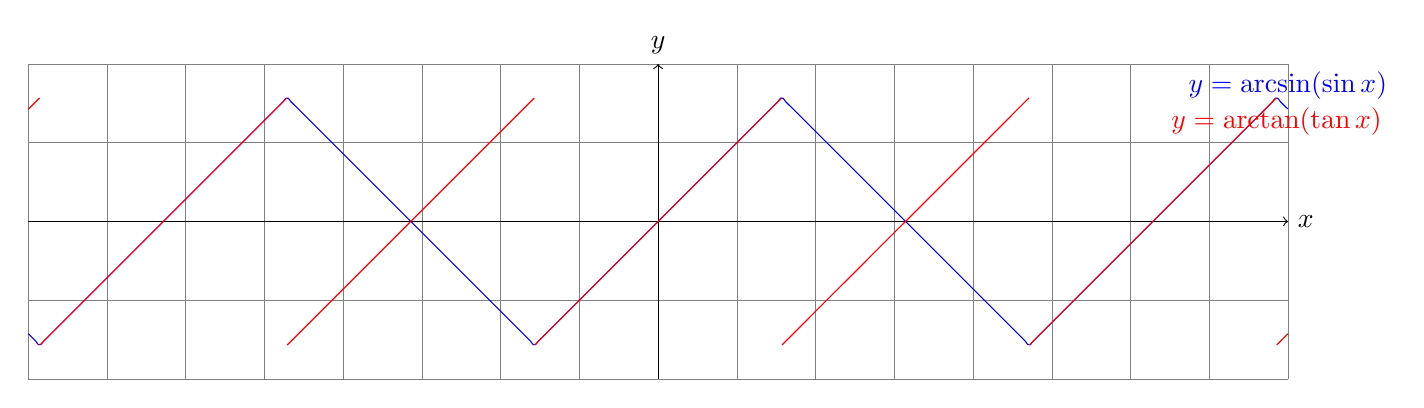
\begin{tikzpicture}[domain=-8:8]
\draw[very thin,color=gray](-8,-2)grid(8,2);
\draw[->](-8,0)--(8,0)node[right]{$x$};
\draw[->](0,-2)--(0,2)node[above]{$y$};
\draw[samples=500,smooth,color=blue]plot(\x,{asin(sin(\x*180/pi))*pi/180})node[above]{$y=\arcsin(\sin{x})$};
\draw[domain=-8:-5*pi/2-1e-3,samples=40,smooth,color=red]plot(\x,{atan(tan(\x*180/pi))*pi/180});
\draw[domain=-5*pi/2+1e-3:-3*pi/2-1e-3,samples=40,smooth,color=red]plot(\x,{atan(tan(\x*180/pi))*pi/180});
\draw[domain=-3*pi/2+1e-3:-pi/2-1e-3,samples=40,smooth,color=red]plot(\x,{atan(tan(\x*180/pi))*pi/180});
\draw[domain=-pi/2+1e-3:pi/2-1e-3,samples=40,smooth,color=red]plot(\x,{atan(tan(\x*180/pi))*pi/180});
\draw[domain=pi/2+1e-3:3*pi/2-1e-3,samples=40,smooth,color=red]plot(\x,{atan(tan(\x*180/pi))*pi/180});
\draw[domain=3*pi/2+1e-3:5*pi/2-1e-3,samples=40,smooth,color=red]plot(\x,{atan(tan(\x*180/pi))*pi/180})node[below]{$y=\arctan(\tan{x})$};
\draw[domain=5*pi/2+1e-3:8,samples=20,smooth,color=red]plot(\x,{atan(tan(\x*180/pi))*pi/180});
\end{tikzpicture}
\end{center}\par
看出来了吧, $\arcsin(\sin{x})$和$x$是不一样的, 所以化简的时候要谨慎, 不是什么情况下都可以随便化简的. 将来我们学到根式积分的时候还会仔细研究这个化简的问题, 这里先不多说了, 我们来讲后面的知识. \par
\subsection{三角恒等变换及其应用}
三角函数积分有个让人非常头疼的地方, 就是积分过程中可能会遇到多种多样的恒等变换. 适当的恒等变换能大幅加快解题的速度; 反之, 不当的恒等变换就有可能会耽误时间. 我会在后面的课程中讲解如何选择适当的恒等变换, 这里我先把基本的恒等变换介绍一下. \par
首先是大家最喜闻乐见的平方和关系. 大家在高中时都学过$\color{red}\sin^{2}{x}+\cos^{2}{x}=1$, 这种操作能有效地把烦人的三角函数变成常数. 但有的时候我们也会选择反过来用, 大家要有这个意识, 有些时候常数可以化成这样的三角函数形式. \par
我们来看这个积分: 
\begin{align*}
\int\frac{1}{\sin^{2}{x}\cos^{2}{x}}\dif{x}
.\end{align*}
这里就可以把分子上的$1$变成$\sin^{2}{x}+\cos^{2}{x}$, 于是就有
\begin{align*}
\int\frac{\sin^{2}{x}+\cos^{2}{x}}{\sin^{2}{x}\cos^{2}{x}}\dif{x}=\int\frac{\dif{x}}{\cos^{2}{x}}+\int\frac{\dif{x}}{\sin^{2}{x}}
.\end{align*}
大家要熟悉$\sec{x}=\frac{1}{\cos{x}},\;\csc{x}=\frac{1}{\sin{x}}$的关系式. 上面这个积分其实就可以写成下面的样子, 然后套基本积分表就可以了. 
\begin{align*}
\int\sec^{2}{x}\dif{x}+\int\csc^{2}{x}\dif{x}=\tan{x}-\cot{x}+C
.\end{align*}\par
除此之外我们还有两个平方差关系: $\color{red}\sec^{2}{x}-\tan^{2}{x}=1,\;\csc^{2}{x}-\cot^{2}{x}=1$. 这个也很常用, 如果你觉得$\sec^{2}{x}$更难处理, 就可以考虑化成$\tan^{2}{x}+1$再处理, 反过来也是这样的. 大家看这个积分: 
\begin{align*}
\int\cot^{2}{x}\dif{x}
.\end{align*}
我们不熟悉这个积分, 但是我们知道$\int\csc^{2}{x}=\tan{x}+C_{1}$对吧. 那么我们就可以考虑通过恒等变换来化成我们容易做的形式. 
\begin{align*}
\int\cot^{2}{x}\dif{x}=\int\csc^{2}{x}\dif{x}-\int\dif{x}=-\cot{x}-x+C
.\end{align*}\par
然后是我们常用的二倍角公式, 包括正弦形式的$\color{red}\sin{2x}=2\sin{x}\cos{x}$、余弦形式的$\color{red}\cos^{2}{x}=\cos^{2}{x}-\sin^{2}{x}$和正切形式的$\tan{2x}=\frac{2\tan{x}}{1-\tan^{2}{x}}$. 这些公式其实都是通过和角公式推导出来的. 那么来看看这个例题: 
\begin{align*}
\int\cos{2x}\sin{x}\cos{x}\dif{x}
.\end{align*}
想必大家已经能想到要怎么做了. 无非就是二倍角公式反过来用两次嘛, 易如反掌. 
\begin{align*}
\int\cos{2x}\sin{x}\cos{x}\dif{x}=\frac{1}{2}\int\sin{2x}\cos{2x}\dif{x}=\frac{1}{4}\int\sin{4x}\dif{x}=-\frac{\cos{4x}}{16}+C
.\end{align*}\par
余弦形式的二倍角公式还可以结合平方和关系推出两个公式: $\color{red}\cos{2x}=2\cos^{2}{x}-1=1-2\sin^{2}{x}$. 我们再把这两个式子变变形, 可以得到
\begin{align*}\color{red}
\cos^{2}{x}=\frac{1+\cos{2x}}{2},\;\sin^{2}{x}=\frac{1-\cos{2x}}{2}
.\end{align*}
这就是传说中的降幂公式. 降幂公式的作用, 我会在后面进行讲解. 这里只举一个简单的例子: 
\begin{align*}
\int\sin^{2}{x}\dif{x}=\int\frac{1-\cos{2x}}{2}\dif{x}=\frac{x}{2}-\frac{\sin{2x}}{4}+C
.\end{align*}\par
和角公式没什么可讲的, 大家高中的时候也都接触过了. 不过和角公式引出的积化和差、和差化积公式还是值得介绍一下的. 这些公式不那么容易记忆, 我也不提倡大家记忆, 但是考试的时候一定要会推导. 公式这种东西, 要么记下来, 要么会熟练推导. 要是都不会, 那就玩完了. \par
接下来我手把手教大家如何推导积化和差公式. 首先我们需要列出如下四个和角公式: 
\begin{align*}
\sin(a+b)={}&\sin{a}\cos{b}+\cos{a}\sin{b}.\tag{1}\\
\sin(a-b)={}&\sin{a}\cos{b}-\cos{a}\sin{b}.\tag{2}\\
\cos(a+b)={}&\cos{a}\cos{b}-\sin{a}\sin{b}.\tag{3}\\
\cos(a-b)={}&\cos{a}\cos{b}+\sin{a}\sin{b}.\tag{4}
\end{align*}
这里我们对$(1)(2)$两式作和作差, 对$(3)(4)$两式作和作差, 就能够得到下面的四个新式子: 
\begin{align*}
\sin(a+b)+\sin(a-b)={}&2\sin{a}\cos{b}.\tag{5}\\
\sin(a+b)-\sin(a-b)={}&2\cos{a}\sin{b}.\tag{6}\\
\cos(a+b)+\cos(a-b)={}&2\cos{a}\cos{b}.\tag{7}\\
\cos(a-b)-\cos(a+b)={}&2\sin{a}\sin{b}.\tag{8}
\end{align*}
尤其要注意, $(8)$式这里我是把$\cos(a-b)$写在前, $\cos(a+b)$写在后的, 这个顺序和前三个不一样. 自行推导的时候千万不要搞错. \par
大家看, $(5)-(8)$这四个式子有双向作用: 我们从左往右推导, 就可以把三角函数和差的形式转换成积的形式; 我们从右往左推导, 就可以把三角函数积的形式转换成和差的形式. 所以这四个式子其实就沟通了和差与积, 也就是我们推导和差化积公式与积化和差公式的基础. \par
我们先来看积化和差, 我们在$(5)-(8)$式中对等号两边同时除$2$, 就可以得到
\begin{align*}\color{red}
\sin{a}\cos{b}={}&\color{red}\frac{\sin(a+b)+\sin(a-b)}{2}.\\\color{red}
\cos{a}\sin{b}={}&\color{red}\frac{\sin(a+b)-\sin(a-b)}{2}.\\\color{red}
\cos{a}\cos{b}={}&\color{red}\frac{\cos(a+b)+\cos(a-b)}{2}.\\\color{red}
\sin{a}\sin{b}={}&\color{red}\frac{\cos(a-b)-\cos(a+b)}{2}
.\end{align*}\par
我们再来看和差化积. 其实$(5)-(8)$式的形式已经是和差化积了, 只不过等号右边是用$a,\,b$来表达的, 而不是用$a+b,\,a-b$来表达的. 其实这很好处理, 因为我们可以把$a$写成$\frac{a+b}{2}+\frac{a-b}{2}$, 把$b$写成$\frac{a+b}{2}-\frac{a-b}{2}$. 
\begin{align*}
\sin(a+b)+\sin(a-b)=2\sin(\frac{a+b}{2}+\frac{a-b}{2})\cos(\frac{a+b}{2}-\frac{a-b}{2}).\\
\sin(a+b)-\sin(a-b)=2\cos(\frac{a+b}{2}+\frac{a-b}{2})\sin(\frac{a+b}{2}-\frac{a-b}{2}).\\
\cos(a+b)+\cos(a-b)=2\cos(\frac{a+b}{2}+\frac{a-b}{2})\cos(\frac{a+b}{2}-\frac{a-b}{2}).\\
\cos(a-b)-\cos(a+b)=2\sin(\frac{a+b}{2}+\frac{a-b}{2})\sin(\frac{a+b}{2}-\frac{a-b}{2})
.\end{align*}
这里写这么多$a+b$和$a-b$不太好看, 我们统一换成$a$和$b$, 就得到了和差化积公式的标准表达: 
\begin{align*}\color{red}
\sin{a}+\sin{b}={}&\color{red}2\sin{\frac{a+b}{2}}\cos{\frac{a-b}{2}}.\\\color{red}
\sin{a}-\sin{b}={}&\color{red}2\cos{\frac{a+b}{2}}\sin{\frac{a-b}{2}}.\\\color{red}
\cos{a}+\cos{b}={}&\color{red}2\cos{\frac{a+b}{2}}\cos{\frac{a-b}{2}}.\\\color{red}
\cos{b}-\cos{a}={}&\color{red}2\sin{\frac{a+b}{2}}\sin{\frac{a-b}{2}}
.\end{align*}\par
除此之外, 我们还需要知道一个线性组合公式: 
\begin{align*}\color{red}
a\sin{x}+b\cos{x}=\sqrt{a^{2}+b^{2}}\sin(x+\arctan{\frac{b}{a}})\;\qty(a>0)
.\end{align*}
这个式子俗称辅助角公式, 很多时候可以用来处理类似的积分: 
\begin{align*}
\int\frac{\dif{x}}{\qty(\sin{x}+\sqrt{3}\cos{x})^{2}}=\int\frac{\dif{x}}{4\sin(x+\frac{\pi}{3})^{2}}={}&\frac{1}{4}\int\csc^{2}\qty(x+\frac{\pi}{3})\dif{\qty(x+\frac{\pi}{3})}\\
={}&-\frac{1}{4}\cot(x+\frac{\pi}{3})+C
.\end{align*}
那么最后我们再来看一个重要的恒等式: 
\begin{align*}\color{red}
2\sin{x}\cos{x}=\qty(\sin{x}+\cos{x})^{2}-1=1-\qty(\sin{x}-\cos{x})^{2}
.\end{align*}
这个公式在组合积分法当中会经常用到, 我们之后再讲. \par
\subsection{同角的三角有理式与齐次三角有理式}
这节课剩的时间不多了, 我来简单讲讲三角有理式. \par
三角有理式, 说白了就是由六大三角函数和若干常数构成的有理函数. 一般我们为了研究方便, 默认这些三角函数都是以$x$为参数的, 或者说它们是同角的. 我举几个例子, 比如
\begin{align*}
\sin{x},\;-\csc^{2}{x},\;\frac{2\sin{x}}{4+3\tan{x}},\;\frac{2\cot{x}}{\sin^{3}{x}+\cos^{3}{x}}
,\end{align*}
都是同角的三角有理式. 角都为$x$嘛. \par
我们来考虑一个问题: 在同角的前提下, 正切、余切、正割、余割函数其实都是由正余弦函数构成的三角有理式, 那么只需要使用正余弦函数构成的有理函数就能够将原来的三角有理式表达出来对吧. 比如说, 上面的四个三角有理式就可以只用正余弦函数表达为
\begin{align*}
\sin{x},\;-\frac{1}{\sin^{2}{x}},\;\frac{2\sin{x}\cos{x}}{4\cos{x}+3\sin{x}},\;\frac{2\cos{x}}{\sin{x}\qty(\sin^{3}{x}+\cos^{3}{x})}
.\end{align*}
正因为只用正余弦函数就可以表达一个三角函数有理式, 所以我们有些时候也把它记成\\$R(\sin{x},\cos{x})$, 意思就是关于$\sin{x}$和$\cos{x}$的有理函数. \par
因为$\sin{x}$也能够用$\cos{x}$与$\tan{x}$的有理式表达, 所以任何一个三角函数有理式都是可以用$\cos{x}$和$\tan{x}$的有理式来表达的, 这个时候我们把它记成$R_{1}(\cos{x},\tan{x})$, 意思是关于$\cos{x}$和$\tan{x}$的有理函数. 不过这个形式我们不常用, 我们更常用的是$R(\sin{x},\cos{x})$. \par
这里我们先来介绍齐次三角多项式的概念. 在只由$\sin{x},\,\cos{x}$构成的三角多项式$P(\sin{x},\cos{x})$中, 如果每一项中$\sin{x}$和$\cos{x}$的次数之和都是同一个常数, 那么我们就把这个三角多项式称为齐次三角多项式. 比如说, 这些就是齐次三角多项式: 
\begin{align*}
\sin{x}+\cos{x},\;\sin^{2}{x}-3\sin{x}\cos{x},\;\sin^{4}{x}+2\sin{x}\cos^{3}{x}-\cos^{4}{x}
.\end{align*}
而这些就不是齐次三角多项式: 
\begin{align*}
1+\sin{x},\;\sin^{3}{x}-\cos^{2}{x},\;1+2\sin^{2}{x}+\cos^{5}{x}
.\end{align*}\par
那么我来考考大家, 三角多项式
\begin{align*}
1+\sin^{2}{x}
\end{align*}
是不是齐次三角多项式呢? 其实它是, 因为这里的常数可以变换成二次三角有理式. 
\begin{align*}
1+\sin^{2}{x}=2\sin^{2}{x}+\cos^{2}{x}
.\end{align*}\par
那么我再来考考大家, 三角多项式
\begin{align*}
1+\cos^{2}{x}-2\sin^{4}{x}
\end{align*}
是不是齐次三角多项式呢? 它也是, 因为常数可以变换成二次或四次三角有理式, 因此
\begin{align*}
1+\cos^{2}{x}-2\sin^{4}{x}={}&\qty(\sin^{2}{x}+\cos^{2}{x})^{2}+\cos^{2}{x}\qty(\sin^{2}{x}+\cos^{2}{x})-2\sin^{4}{x}\\
={}&-\sin^{4}{x}+3\sin^{2}{x}\cos^{2}{x}+2\cos^{4}{x}
.\end{align*}\par
齐次三角有理式, 简单说就是可以表示为两个齐次三角多项式之商的三角有理式. 比如说
\begin{align*}
\frac{1}{\sin{x}-2\cos{x}},\;\frac{\sin{x}\cos{x}-2}{\sin^{3}{x}+\cos^{3}{x}},\;\frac{\sin{x}}{3\sin{x}-\cos^{3}{x}},\;\sin{x}+\frac{1}{\sin{x}+\cos{x}}
.\end{align*}
第一个大家一眼就能看出来. 第二个需要把分子变成$\sin{x}\cos{x}-2\sin^{2}{x}-2\cos^{2}{x}$; 同理, 第三个需要把分母变成$3\sin^{3}{x}+3\sin{x}\cos^{2}{x}-\cos^{3}{x}$. 而第四个呢, 需要先通分, 再对分子做变换, 我就不具体写了. \par
齐次三角有理式有很多非常好的性质, 我们在后面边讲边介绍. \par
\section{三角函数积分的有理化}
大部分情况下, 我们遇到的三角函数积分都可以通过适当变形和换元转化为有理函数, 进而按照有理函数的积分法来解决. 因为有理函数积分都是有解的, 所以三角有理式的积分都是可解的. \par
这节课我就围绕着三角函数积分的有理化问题, 给大家讲解三角函数积分的通用做法. \par
\subsection{同角化}
我们在上节课介绍了三角有理式. 我们介绍的三角有理式都有一个默认的前提: 所有三角函数的参数都是相同的 (比如$x$) . 但是出题人没那么多规矩, 他可以给你出各种花式的三角函数积分, 比如说
\begin{align*}
\int\frac{\sin{3x}\sin(\pi x+1)}{\sin{x}}\dif{x}
.\end{align*}
大家以目前的水平不需要做这道题, 我写这题只是为了给大家开开眼界. \par
当我们遇到一道三角函数积分的时候呢, 我们首先应该看看其中的每个三角函数是否都是相同参数的. 我们先来考虑一下, 我们可能遇到哪些种类的非同角情形, 然后再针对性地想办法解决. \par
第一种情形比较简单, 就是被积函数的各个角度之间都是整数倍关系, 比如
\begin{align*}
\sin{2x}\sin{x},\;\cos{2x}\sin^{2}{x}
.\end{align*}
这种时候我们只需要通过倍角公式来化简就可以了. 比如说
\begin{align*}
{}&\sin{2x}\sin{x}=2\sin^{2}{x}\cos{x}.\\
{}&\cos{2x}\sin^{2}{x}=\sin^{2}{x}\cos^{2}{x}-\sin^{4}{x}
.\end{align*}
也有些时候可以用半角公式, 比如说
\begin{align*}
\cos{2x}\sin^{2}{x}=\frac{1}{2}\cos{2x}\qty(1-\cos{2x})=\frac{1}{2}\cos{2x}-\frac{1}{2}\cos^{2}{2x}
.\end{align*}
等到大家学完有理化之后就会明白, 第二个式子用半角公式做比用倍角公式做起来要快. 但不是所有的时候使用半角公式都很合适. 我就拿第一个例子来讲, 如果用半角公式, 就会得到
\begin{align*}
\sin{2x}\sin{x}=\pm\sin{2x}\sqrt{\frac{1-\cos{2x}}{2}}
.\end{align*}
我觉得这里不需要我说大家也能看出来, 这个地方用了半角公式之后, 形式变得更丑陋了. 我们既要处理根号, 还要分区间讨论正负号的问题, 这不是自找麻烦吗? \par
我给大家介绍个原则: 同角化的过程中, 首先要避免出现那些处理起来很麻烦的结构, 比如说正负号和根号. 你们看$\sin{x}=\pm\sqrt{\frac{1-\cos{2x}}{2}}$就不是一个好的处理思路, 因为既有正负号又有根号; 而$\sin^{2}{x}=\frac{1+\cos{2x}}{2}$就没问题, 因为没产生难以处理的结构. \par
其次还要考虑一点, 就是别让三角函数的次数太高. 大家可以看到, 同样的一个式子, 我化成$\sin^{2}{x}\cos^{2}{x}-\sin^{4}{x}$或者$\frac{\cos{2x}-\cos^{2}{2x}}{2}$在式子复杂程度上是有区别的. 前者最高可以到四次, 后者最高只有二次, 后者处理起来就比前者要轻松很多. \par
我们再来考虑第二种情形, 被积函数的各个角度之间只相差常数, 比如
\begin{align*}
\sin{x}\cos(x+\frac{\pi}{6}),\;\frac{\sin{x}}{\sin(x+\frac{\pi}{4})}
.\end{align*}
这种问题其实不难处理, 和角公式用起来就行, 比如说
\begin{align*}
{}&\sin{x}\cos(x+\frac{\pi}{6})=\sin{x}\qty(\frac{\sqrt{3}}{2}\cos{x}-\frac{1}{2}\sin{x})=\frac{\sqrt{3}}{2}\sin{x}\cos{x}-\frac{1}{2}\sin^{2}{x}.\\
{}&\frac{\sin{x}}{\sin(x+\frac{\pi}{4})}=\frac{\sqrt{2}\sin{x}}{\sin{x}+\cos{x}}
.\end{align*}\par
不过我要补充一下, 第二个式子还有一种处理方法. 我先令$t=x+\frac{\pi}{4}$, 然后把它变成关于$t$的式子. 
\begin{align*}
\frac{\sin{x}}{\sin(x+\frac{\pi}{4})}=\frac{\sin(t-\frac{\pi}{4})}{\sin{t}}=\frac{\sin{t}-\cos{t}}{\sqrt{2}\sin{t}}=\frac{1}{\sqrt{2}}-\frac{1}{\sqrt{2}}\cot{t}
.\end{align*}
我们来比较一下, $\frac{\sqrt{2}\sin{x}}{\sin{x}+\cos{x}}$和$\frac{\sin{t}-\cos{t}}{\sqrt{2}\sin{t}}$, 这二者有一个显著的差别: 前者的分母是多项式, 而后者的分母是单项式. 我在这里也给大家指个北: 在三角函数积分当中, 尽量尝试把分母化成单项式. \par
单项式有什么好处呢? 就是容易分项以及去分母. 比如说$\frac{\sqrt{2}\sin{x}}{\sin{x}+\cos{x}}$, 这个就很难分项, 分母放着一个多项式也去不掉; 但是$\frac{\sin{t}-\cos{t}}{\sqrt{2}\sin{t}}$就不一样了, 我不仅可以直接分项, 还可以把$\frac{\cos{t}}{\sin{t}}$变成$\cot{t}$, 整理一下就化成一个不含分母的形状$\frac{1}{\sqrt{2}}-\frac{1}{\sqrt{2}}\cot{t}$. \par
接下来考虑第三种情况: 被积函数的各个角度之间是非整数倍关系, 比如
\begin{align*}
\sin{x}\sin{\pi x},\;\sin{x}\cos{x}\cos{\pi x}
.\end{align*}
对于这类问题, 我们选用积化和差公式来解决. \par
为什么要使用积化和差呢? 这是因为我们发现, 上面讲过的所有方法都没办法进行同角化了. 但是我们还有一个策略: 如果实在无法同角化, 我们就把不一样的角度通过分项积分的方法, 放到两个积分当中. 比如说吧, 第一个式子可以这么变: 
\begin{align*}
\sin{x}\sin{\pi x}=\frac{\cos[\qty(\pi-1)x]-\cos[\qty(\pi+1)x]}{2}
.\end{align*}
那么把这个函数作为被积函数, 我们会发现, 我们现在只需要分别处理这两个积分就可以了: 
\begin{align*}
\int\cos[\qty(\pi-1)x]\dif{x},\;\int\cos[\qty(\pi+1)x]\dif{x}
.\end{align*}
大家看, 这两个积分各自都是同角的吧——只有一个角当然算同角了. 虽然没有严格意义上化为同角, 但是我们可以曲线救国, 通过分项的方法得到两个同角的积分. \par
那么我们再来看看$\sin{x}\cos{x}\cos{\pi x}$这个式子如何处理. 这里想直接套用积化和差公式的话, 需要做三步积化和差操作. 为了方便计算, 我们可以先把这个式子用二倍角公式化简一下, 再套积化和差公式. 思考问题要灵活. 
\begin{align*}
\sin{x}\cos{x}\cos{\pi x}=\frac{1}{2}\sin{2x}\cos{\pi x}=\frac{1}{4}\sin[\qty(2+\pi)x]+\frac{1}{4}\sin[\qty(2-\pi)x]
.\end{align*}
好, 我们在这一步完成了同角化之后, 就可以应用后面所介绍的诸多解题方法了. 请听下回分解. \par
\subsection{正余弦函数类有理化}
先介绍一个来自代数学的定理: 如果有理函数$R(x,y)$满足$R(-x,y)=-R(x,y)$, 那么这个函数可以改写成$R_{1}(x^{2},y)x$的形式. 说人话就是, 如果有理函数$f(x)$是关于$x$的奇函数, 那么这个函数可以改写成关于$x^{2}$的有理函数$g(x^{2})$再乘上一个$x$. 举几个例子吧, 有理函数
\begin{align*}
\frac{x^{3}+x}{x^{2}+4},\;\frac{x^{2}+1}{x^{3}}
\end{align*}
都是关于$x$的奇函数. 而它们分别可以改写成
\begin{align*}
\frac{\qty(x^{2})+1}{\qty(x^{2})+4}x,\;\frac{\qty(x^{2})+1}{\qty(x^{2})^{2}}x
.\end{align*}\par
有了这点基础, 我们来研究积分
\begin{align*}
\int R(\sin{x},\cos{x})\dif{x}
\end{align*}
当中一些特殊的类型. \par
如果三角有理式$R(\sin{x},\cos{x})$满足$R(\sin{x},-\cos{x})=-R(\sin{x},\cos{x})$, 那么这个有理式就可以改写成$R_{1}(\sin{x},\cos^{2}{x})\cos{x}$. 于是原积分就可以改写为
\begin{align*}
\int R_{1}(\sin{x},\cos^{2}{x})\cos{x}\dif{x}=\int R_{1}(\sin{x},1-\sin^{2}{x})\dif{\sin{x}}
.\end{align*}
发现了吗, 这下只剩下$\sin{x}$了. 那么我们换元$u=\sin{x}$, 就可以得到
\begin{align*}
\int R_{1}(u,1-u^{2})\dif{u}
.\end{align*}
这不就是个有理函数积分吗! 秒了. \par
而如果三角有理式$R(\sin{x},\cos{x})$满足$R(-\sin{x},\cos{x})=-R(\sin{x},\cos{x})$, 那么这个有理式就可以改写成$R_{1}(\sin^{2}{x},\cos{x})\sin{x}$. 于是原积分就可以改写为
\begin{align*}
\int R_{1}(\sin^{2}{x},\cos{x})\sin{x}\dif{x}=-\int R_{1}(1-\cos^{2}{x},\cos{x})\dif{\cos{x}}
.\end{align*}
同样的道理, 我们只要换元$u=\cos{x}$, 就可以得到
\begin{align*}
-\int R_{1}(1-u^{2},u)\dif{u}
.\end{align*}
这也就是个有理函数积分, 秒了. \par
光说不练假把式, 我出一道题大家练练: 
\begin{align*}
\int\frac{\dif{x}}{\cos{x}}=\int\sec{x}\dif{x}
.\end{align*}
这道题的被积函数是关于$\cos{x}$的奇函数, 所以我们需要这样凑: 
\begin{align*}
\int\frac{\dif{x}}{\cos{x}}=\int\frac{\cos{x}\dif{x}}{\cos^{2}{x}}=\int\frac{\dif{\sin{x}}}{1-\sin^{2}{x}}=\frac{1}{2}\ln\qty|\frac{1+\sin{x}}{1-\sin{x}}|+C
.\end{align*}
顺便插一句, 这个结果可以通过恒等变换化成$\ln\qty|\sec{x}+\tan{x}|+C$, 这个形式是最常用的. 具体证明就留给你们当作业好了. \par
再来看一道题: 
\begin{align*}
\int\frac{\sin{x}+\cos{x}}{2\sin^{2}{x}-\cos^{2}{x}}\dif{x}
.\end{align*}
这题我们乍一看可能没什么思路是吧, 但是如果我们分项来思考的话呢, 问题就会迎刃而解: 
\begin{align*}
\int\frac{\sin{x}+\cos{x}}{2\sin^{2}{x}-\cos^{2}{x}}\dif{x}=\int\frac{\sin{x}\dif{x}}{2\sin^{2}{x}-\cos^{2}{x}}+\int\frac{\cos{x}\dif{x}}{2\sin^{2}{x}-\cos^{2}{x}}
.\end{align*}
我们分别来看这两个积分, 第一个是关于$\sin{x}$的奇函数, 而第二个是关于$\cos{x}$的奇函数, 这不就做出来了吗? 
\begin{align*}
\int\frac{\sin{x}\dif{x}}{2\sin^{2}{x}-\cos^{2}{x}}={}&\int\frac{-\dif{\cos{x}}}{2-3\cos^{2}{x}}\\
\int\frac{\cos{x}\dif{x}}{2\sin^{2}{x}-\cos^{2}{x}}={}&\int\frac{\dif{\sin{x}}}{3\sin^{2}{x}-1}
.\end{align*}
所以说啊, 分而治之的思想很重要. 你把一大堆东西放在一块不好处理的话, 那就要逐个击破. \par
\subsection{正切函数类有理化}
再介绍另一个来自代数学的定理: 如果有理函数$R(x,y)$满足$R(-x,y)=R(x,y)$, 那么这个函数可以改写成$R_{1}(x^{2},y)$的形式. 说人话就是, 如果有理函数$f(x)$是关于$x$的偶函数, 那么这个函数可以改写成关于$x^{2}$的有理函数$g(x^{2})$. 举几个例子吧, 有理函数
\begin{align*}
x^{6},\;\frac{x^{2}}{x^{4}+1}
\end{align*}
都是关于$x$的偶函数. 而它们分别可以改写成
\begin{align*}
\qty(x^{2})^{3},\;\frac{\qty(x^{2})}{\qty(x^{2})^{2}+1}
.\end{align*}\par
我们再来看积分
\begin{align*}
\int R(\sin{x},\cos{x})\dif{x}
\end{align*}
的另一种情况: $R(-\sin{x},-\cos{x})=R(\sin{x},\cos{x})$. \par
这个时候我们需要改变一下这个三角有理式的表达形式了. 我在之前提过一句, 因为$\sin{x}=\cos{x}\tan{x}$, 所以$R(\sin{x},\cos{x})$又可以换种表达方式, 写成$R_{1}(\cos{x},\tan{x})$. 那么我们再对上面的关系式变形一下看看会得到什么吧. :
\begin{align*}
R(-\sin{x},-\cos{x})=R_{1}(-\cos{x},\tan{x})=R_{1}(\cos{x},\tan{x})=R(\sin{x},\cos{x})
.\end{align*}
第一个等号处应该不难理解吧, 这是因为当$\sin{x},\,\cos{x}$分别变成$-\sin{x},-\cos{x}$的时候, 式子里的$\tan{x}=\frac{\sin{x}}{\cos{x}}=\frac{-\sin{x}}{-\cos{x}}$是不变的. \par
于是我们得到了一个新的关系式: 
\begin{align*}
R_{1}(-\cos{x},\tan{x})=R_{1}(\cos{x},\tan{x})
.\end{align*}
于是按照我们之前的分析, 我就可以把这个三角有理式改写成$R_{2}\qty(\cos^{2}{x},\tan{x})$的形式. \par
我们再来分析一下, 其实$\cos^{2}{x}$能表示为$\tan{x}$的有理式: 
\begin{align*}
\cos^{2}{x}=\frac{1}{\sec^{2}{x}}=\frac{1}{\tan^{2}{x}+1}
.\end{align*}\par
既然$R_{2}\qty(\frac{1}{\tan^{2}{x}+1},\tan{x})$已经是关于$\tan{x}$的有理式了, 那么我直接改写成$R_{3}(\tan{x})$行吧. 
到现在为止我们已经绕了这么一大圈, 把原来的积分式变形成了
\begin{align*}
\int R_{3}(\tan{x})\dif{x}
.\end{align*}
最后一步, 我们换元$u=\tan{x}$, 反解出$x=\arctan{u}+k\pi,\;\qty(k\in\mathbb{Z})$. 所以
\begin{align*}
\int R_{3}(\tan{x})\dif{x}=\int R_{3}(u)\dif{\qty(\arctan{u}+k\pi)}=\int R_{3}(u)\dif{\arctan{u}}=\int\frac{R_{3}(u)\dif{u}}{u^{2}+1}
.\end{align*}
好了, 大功告成, 我们把有理化做完了. \par
接下来出几道题给大家练练: 
\begin{align*}
\int\frac{\dif{x}}{\sin^{2}{x}+2\cos^{2}{x}}
.\end{align*}
这题显然是刚才介绍的类型吧, 所以我们凑$\dif{\tan{x}}$. 不过我们做题的时候没必要那么思维僵化, 只要能做出来就行了. 所以我们第一步就对分子分母同乘$\sec^{2}{x}$, 这样做的好处是让分母上$\sin^{2}{x}$变成$\tan^{2}{x}$, 而$2\cos^{2}{x}$直接变成常数了. 
\begin{align*}
\int\frac{\dif{x}}{\sin^{2}{x}+2\cos^{2}{x}}=\int\frac{\sec^{2}{x}\dif{x}}{\tan^{2}{x}+2}
.\end{align*}
接下来我们发现我们可以直接凑微分了, 因为$\sec^{2}{x}\dif{x}=\dif{\tan{x}}$. 那么我们只需要再换元$u=\tan{x}$就可以得到
\begin{align*}
\int\frac{\dif{u}}{u^{2}+2}=\frac{1}{\sqrt{2}}\arctan{\frac{u}{\sqrt{2}}}+C
.\end{align*}\par
再来一题: 
\begin{align*}
\int\frac{\sin{x}}{\sin{x}+\cos{x}}\dif{x}
.\end{align*}
首先我们要记得判断一下它的被积函数是不是我们研究过的类型, 别二话不说直接上手. 如果拿着一个套路化了老半天突然发现条件对不上, 那这不是白费吗? \par
我们发现
\begin{align*}
\frac{-\sin{x}}{-\sin{x}-\cos{x}}=\frac{\sin{x}}{\sin{x}+\cos{x}}
\end{align*}
满足我们刚才介绍的情况, 所以应该凑$\dif{\tan{x}}$. 怎么凑呢? 我们来做一下. 首先我们对分子分母同乘$\sec{x}$, 这样做是为了把$\sin{x}$变成$\tan{x}$, 把$\cos{x}$变为常数. 
\begin{align*}
\int\frac{\sin{x}\dif{x}}{\sin{x}+\cos{x}}=\int\frac{\tan{x}\dif{x}}{\tan{x}+1}
.\end{align*}
接下来我们对分子分母同乘$\sec^{2}{x}$, 这是为了在分子上实现微分变换$\sec^{2}{x}\dif{x}=\dif{\tan{x}}$. 
\begin{align*}
\int\frac{\tan{x}\sec^{2}{x}\dif{x}}{\sec^{2}{x}\qty(\tan{x}+1)}=\int\frac{\tan{x}\dif{\tan{x}}}{\qty(\tan{x}+1)\qty(\tan^{2}{x}+1)}
.\end{align*}
这样一来我们其实就实现了有理化的工作. 如果你看着这个积分的形式觉得比较难看, 可以换元$u=\tan{x}$化成
\begin{align*}
\int\frac{u\dif{u}}{\qty(u+1)\qty(u^{2}+1)}
.\end{align*}
剩下的是一道有理积分, 大家裂项就可以做, 当作业好了. \par
再来一题: 
\begin{align*}
\int\frac{\dif{x}}{\sin^{4}{x}+\cos^{4}{x}}
.\end{align*}
这题很显然也是同一个类型, 我们凑$\dif{\tan{x}}$. 先对分子分母同乘$\sec^{4}{x}$, 这样做是为了把$\sin^{4}{x}$变成$\tan^{4}{x}$, 把$\cos^{4}{x}$变为常数. 
\begin{align*}
\int\frac{\dif{x}}{\sin^{4}{x}+\cos^{4}{x}}=\int\frac{\sec^{4}{x}\dif{x}}{\tan^{4}{x}+1}
.\end{align*}
分子上分出一个$\sec^{2}{x}$因子可以用来凑微分. 
\begin{align*}
\int\frac{\sec^{4}{x}\dif{x}}{\tan^{4}{x}+1}=\int\frac{\tan^{2}{x}+1}{\tan^{4}{x}+1}\dif{\tan{x}}
.\end{align*}
这样只要换元$u=\tan{x}$就完成了有理化. \par
哎, 问一下大家, 积分$\int\frac{u^{2}+1}{u^{4}+1}\dif{u}$怎么做来着? 同除$u^{2}$再对勾换元是吧. 
\begin{align*}
\int\frac{u^{2}+1}{u^{4}+1}\dif{u}=\int\frac{1+u^{-2}}{u^{2}+u^{-2}}\dif{u}=\int\frac{\dif{\qty(u-u^{-1})}}{\qty(u-u^{-1})^{2}+2}=\frac{1}{\sqrt{2}}\arctan{\frac{\tan^{2}{x}-1}{\sqrt{2}\tan{x}}}+C
.\end{align*}
是不是轻而易举、手到擒来、易如反掌, 三下五除二就解决了, 简直不在话下啊. \par
\subsection{万能公式方法}
之前我们介绍了两类特殊的积分: 一类是被积函数满足
\begin{align*}
R(-\sin{x},\cos{x})=-R(\sin{x},\cos{x})
\end{align*}
或者
\begin{align*}
R(\sin{x},-\cos{x})=-R(\sin{x},\cos{x})
\end{align*}
的积分, 这种积分可以凑$\dif{\cos{x}}$或者$\dif{\sin{x}}$; 另一类是被积函数满足
\begin{align*}
R(-\sin{x},-\cos{x})=R(\sin{x},\cos{x})
\end{align*}
的积分, 这种积分可以凑$\dif{\tan{x}}$. 接下来我们介绍一下一般的类型, 也就是任意的三角有理式积分$\int R(\sin{x},\cos{x})\dif{x}$. 这类积分存在万能的解题方法, 所以很多人管它叫做万能公式. \par
现在我应用二倍角公式
\begin{align*}
\sin{x}=2\sin{\frac{x}{2}}\cos{\frac{x}{2}},\;\cos{x}=\cos^{2}{\frac{x}{2}}-\sin^{2}{\frac{x}{2}}
\end{align*}
把原来关于$\sin{x},\,\cos{x}$的三角有理式积分化为$R\qty(2\sin{\frac{x}{2}}\cos{\frac{x}{2}},\,\cos^{2}{\frac{x}{2}}-\sin^{2}{\frac{x}{2}})$. 我们发现它还是一个三角有理式对吧? 那我不妨改写成$R_{1}\qty(\sin{\frac{x}{2}},\cos{\frac{x}{2}})$吧. \par
大家可以发现, $R_{1}\qty(\sin{\frac{x}{2}},\cos{\frac{x}{2}})$有良好的性质: 
\begin{align*}
R_{1}\qty(-\sin{\frac{x}{2}},-\cos{\frac{x}{2}})=R\qty(2\sin{\frac{x}{2}}\cos{\frac{x}{2}},\,\cos^{2}{\frac{x}{2}}-\sin^{2}{\frac{x}{2}})=R_{1}\qty(\sin{\frac{x}{2}},\cos{\frac{x}{2}})
.\end{align*}
这意味着什么呢? 我们可以套用上一节的结论: 凑微分$\dif{\tan{\frac{x}{2}}}$来解决问题. \par
我们来道例题吧, 积分
\begin{align*}
\int\frac{\dif{x}}{\sin{x}+\cos{x}}
.\end{align*}
我们对这个被积函数应用二倍角公式, 得到
\begin{align*}
\int\frac{\dif{x}}{2\sin{\frac{x}{2}}\cos{\frac{x}{2}}+\cos^{2}{\frac{x}{2}}-\sin^{2}{\frac{x}{2}}}
.\end{align*}
接下来就是老套路了, 我们对分子分母同乘$\sec^{2}{\frac{x}{2}}$, 于是得到
\begin{align*}
\int\frac{\sec^{2}{\frac{x}{2}}\dif{x}}{-\tan^{2}{\frac{x}{2}}+2\tan{\frac{x}{2}}+1}=-\int\frac{\dif{\tan{\frac{x}{2}}}}{\tan^{2}{\frac{x}{2}}-2\tan{\frac{x}{2}}-1}
.\end{align*}
这样就完成了有理化. \par
再来一道复杂一点的: 
\begin{align*}
\int\frac{1+\sin{x}}{\sin{x}\qty(1+\cos{x})}\dif{x}
.\end{align*}
这题看上去就不太好做的样子, 我们试一下就会发现, 这题的被积函数既不是关于$\sin{x}$或者$\cos{x}$的奇函数, 也不能在$\sin{x},\,\cos{x}$取反后保持不变. 那么只能用万能公式来做. 先套个二倍角公式: 
\begin{align*}
\int\frac{1+\sin{x}}{\sin{x}\qty(1+\cos{x})}\dif{x}=\int\frac{1+2\sin{\frac{x}{2}}\cos{\frac{x}{2}}}{2\sin{\frac{x}{2}}\cos{\frac{x}{2}}\qty(2\cos^{2}{\frac{x}{2}})}\dif{x}
.\end{align*}
我们观察一下, 现在我们把被积函数变成了分子是二次三角多项式, 分母是四次三角多项式的情况. 接下来我们要对分子分母同乘$\sec^{4}{\frac{x}{2}}$, 就会变成这样. 
\begin{align*}
\int\frac{\sec^{2}{\frac{x}{2}}\qty(\tan^{2}{\frac{x}{2}}+2\tan{\frac{x}{2}}+1)}{4\tan{\frac{x}{2}}}\dif{x}
.\end{align*}
这下就好办了, 分母上有$\sec^{2}{\frac{x}{2}}$因子, 我们可以拿来凑个微分, 把它变成
\begin{align*}
\int\frac{\tan^{2}{\frac{x}{2}}+2\tan{\frac{x}{2}}+1}{2\tan{\frac{x}{2}}}\dif{\tan{\frac{x}{2}}}
.\end{align*}
于是我们就完成了有理化. \par
这类问题做多了之后呢, 我们可以总结出一个套路. 在积分$\int R(\sin{x},\cos{x})\dif{x}$之中, 我们只要换元
\begin{align*}\color{red}
\sin{x}={}&\color{red}\frac{2t}{1+t^{2}},\\\color{red}
\cos{x}={}&\color{red}\frac{1-t^{2}}{1+t^{2}},\\\color{red}
\dif{x}={}&\color{red}\frac{2\dif{t}}{1+t^{2}}
.\end{align*}
就可以直接完成有理化的操作. 比如说在上一题当中, 我们通过这样的换元就能够得到
\begin{align*}
\int\frac{1+\sin{x}}{\sin{x}\qty(1+\cos{x})}\dif{x}=\int\frac{1+\frac{2t}{1+t^{2}}}{\frac{2t}{1+t^{2}}(1+\frac{1-t^{2}}{1+t^{2}})}\cdot\frac{2\dif{t}}{1+t^{2}}
.\end{align*}
上述换元就是大名鼎鼎的万能公式. \par
其实万能公式的本质也是通过二倍角公式来推导的, 我现在简单写一下推导过程, 你们先别催我下课啦. \par
\begin{align*}
{}&\sin{x}=2\sin{\frac{x}{2}}\cos{\frac{x}{2}}=\frac{2\tan{\frac{x}{2}}}{\sec^{2}{\frac{x}{2}}}=\frac{2\tan{\frac{x}{2}}}{1+\tan^{2}{\frac{x}{2}}}.\\
{}&\cos{x}=\cos^{2}{\frac{x}{2}}-\sin^{2}{\frac{x}{2}}=\frac{1-\tan^{2}{\frac{x}{2}}}{\sec^{2}{\frac{x}{2}}}=\frac{1-\tan^{2}{\frac{x}{2}}}{1+\tan^{2}{\frac{x}{2}}}.\\
{}&\dif{x}=2\dif{\frac{x}{2}}=2\dif{\qty[\arctan(\tan{\frac{x}{2}})+k\pi]}=2\dif{\qty[\arctan(\tan{\frac{x}{2}})]}=\frac{2\dif{\qty(\tan{\frac{x}{2}})}}{1+\tan^{2}{\frac{x}{2}}}
.\end{align*}
这样一来我们只要换元$t=\tan{\frac{x}{2}}$就可以得到上面的万能公式了. \par
\section{解题技巧}
上节课我们讲了三角函数积分的有理化方法, 包含两种特殊的换元和一种通用的换元. 有了这些方法之后呢, 三角函数积分的问题都能够得到解决. \par
然而, 通用的方法往往有一个弊端, 就是效率低下. 这是个普遍规律, 很多快捷的方法适用范围太窄了, 解决不了一般的问题; 而通用的方法呢, 为了解决一般问题, 只能去牺牲特殊问题的解题效率. 比如说积分$\int\frac{x^{2}-1}{x^{4}+1}\dif{x}$吧, 你要是用裂项的做法那就太慢了, 还是对勾换元好一点. \par
那么我们要想加快解题的速度, 就有两种途径可走: 一是改进通用方法的解题过程, 让它简洁一点, 不那么容易算错数; 二是发掘一些特殊情况并思考有没有一类适用范围窄但是可以快速解决这类问题的方法. 今天这节课我就想讲讲后一种情况. \par
\subsection{降幂公式的使用}
我们先来看一些高次正余弦函数的积分, 比如: 
\begin{align*}
\int\sin^{3}{x}\dif{x},\;\int\cos^{4}{x}\dif{x},\;\int\sin^{2}{x}\cos^{4}{x}\dif{x}
.\end{align*}\par
第一个其实很好解决, 因为它是关于$\sin{x}$的奇函数. 既然如此, 我们凑个$\dif{\cos{x}}$就行了. 
\begin{align*}
\int\sin^{3}{x}=\int\qty(\cos^{2}{x}-1)\dif{\cos{x}}=\frac{1}{3}\cos^{3}{x}-\cos{x}+C
.\end{align*}
第二个和第三个就不那么容易解决了. 如果用凑$\dif{\tan{x}}$的方法, 我们将分别得到
\begin{align*}
\int\frac{\dif{\tan{x}}}{\qty(\tan^{2}{x}+1)^{3}},\;\int\frac{\tan^{2}{x}\dif{\tan{x}}}{\qty(\tan^{2}{x}+1)^{4}}
.\end{align*}
这个有理函数积分的难度非常高, 这么搞实在没必要. 后面我还会讲到, 判断被积函数的次数有利于帮助你们估计有理化的难度. \par
我们先来研究一个相对简单的类型, 这里我们选择降幂公式来操作: 
\begin{align*}
\int\sin^{2}{x}\dif{x}=\int\frac{1-\cos{2x}}{2}\dif{x}=\frac{1}{2}\int\dif{x}-\frac{1}{4}\int\cos{2x}\dif{2x}
.\end{align*}
后面就简单了. \par
那么我们就顺着降幂公式的思路, 来解决一下积分$\int\cos^{4}{x}\dif{x}$试试. 我们可以把$\cos^{4}{x}$看作是$\qty(\cos^{2}{x})^{2}$, 这样的话就会有
\begin{align*}
\int\qty(\cos^{2}{x})^{2}\dif{x}=\int\qty(\frac{1-\cos{2x}}{2})^{2}\dif{x}=\frac{1}{4}\int\dif{x}-\frac{1}{2}\int\cos{2x}\dif{x}+\frac{1}{4}\int\cos^{2}{2x}\dif{x}
.\end{align*}
我们看一下, 现在我们把这个问题化成了三个子问题. 其中$\int\dif{x}$和$\int\cos{2x}\dif{x}$是很容易解决的, 对吧? 那么积分$\int\cos^{2}{2x}\dif{x}$要怎么解决呢? 我们可以继续使用降幂公式. 
\begin{align*}
\int\cos^{2}{2x}\dif{x}=\int\frac{1+\cos{4x}}{2}\dif{x}=\frac{1}{2}\int\dif{x}+\frac{1}{2}\int\cos{4x}\dif{x}
.\end{align*}
这里我们通过两次使用降幂公式将所有高次的积分都变成了一次的. 其实不一定非要都变成一次, 只要变成像$\int\sin^{3}{x}\dif{x}$那样的奇数次, 就可以很容易地完成有理化了. \par
现在我们来拿最后一题开刀吧. 
\begin{align*}
\int\sin^{2}{x}\cos^{4}{x}\dif{x}={}&\int\qty(\frac{1-\cos{2x}}{2})\qty(\frac{1+\cos{2x}}{2})^{2}\dif{x}\\
={}&-\frac{1}{8}\int\cos^{3}{2x}\dif{x}-\frac{1}{8}\int\cos^{2}{2x}\dif{x}+\frac{1}{8}\int\cos{2x}\dif{x}+\frac{1}{8}\int\dif{x}
.\end{align*}
我先写到这里. 大家来看哈, 现在的四个子问题当中, $\int\cos{x}\dif{x}$和$\int\dif{x}$可以直接做了, 而$\int\cos^{3}{2x}\dif{x}$呢, 这个被积函数是关于$\cos{2x}$的奇函数, 那么直接有理化就行了. \par
最后分析$\int\cos^{2}{2x}\dif{x}$, 我们可以再用一次降幂公式, 我懒得写了你们自己做. \par
总结起来就是, 遇到偶数次的就用降幂公式, 如果降幂之后仍然有偶数次的项, 就继续用降幂公式, 直到全都降成奇数次幂为止. 对于奇数次幂呢, 就很好办了, 直接凑微分有理化就行. \par
其实呢, 降幂公式不仅能在齐次三角多项式里用, 放到齐次三角有理分式中也没问题. 不过呢, 这种情况一般要就题论题, 因为有些时候用降幂公式反而更难做了. 另外, 用降幂公式就意味着要保证被积函数整体是偶数次的, 奇数次的就不能用了. 我举一个例题: 
\begin{align*}
\int\frac{\sin^{3}{x}+\sin^{2}{x}\cos{x}}{\cos{x}-\sin{x}}\dif{x}=\int\frac{\sin^{2}{x}\qty(\sin{x}+\cos{x})^{2}}{\cos^{2}{x}-\sin^{2}{x}}\dif{x}
.\end{align*}
平方差的步骤是为了让分母能变形成一个$\cos{2x}$. 大家看到了, 这个是单项式, 分母是单项式就会很舒服. 接下来可以直接套用降幂公式了. 
\begin{align*}
{}&\int\frac{\sin^{2}{x}\qty(\sin{x}+\cos{x})^{2}}{\cos^{2}{x}-\sin^{2}{x}}\dif{x}\\
={}&\frac{1}{2}\int\frac{\qty(1-\cos{2x})\qty(1+\sin{2x})}{\cos{2x}}\dif{x}\\
={}&\frac{1}{2}\int\sec{2x}\dif{x}-\frac{1}{2}\int\dif{x}+\frac{1}{2}\int\tan{2x}\dif{x}-\frac{1}{2}\int\sin{2x}\dif{x}\\
={}&\frac{1}{4}\ln\qty|\sec{2x}+\tan{2x}|-\frac{x}{2}-\frac{1}{4}\ln\qty|\cos{2x}|+\frac{1}{4}\cos{2x}+C
.\end{align*}\par
我再举个降幂公式帮倒忙的例子, 比如说
\begin{align*}
\int\frac{\dif{x}}{\cos^{6}{x}}=8\int\frac{\dif{x}}{\qty(1+\cos{2x})^{3}}
.\end{align*}
本来被积函数是齐次的, 分母还是单项式; 结果你来套一个降幂公式, 被积函数也不齐次了, 分母也不是单项式了, 何苦呢? \par
\subsection{欧拉公式降幂方法}
用降幂公式解决形如
\begin{align*}
\int\sin^{2n}{x}\cos^{2m}{x}\dif{x}
\end{align*}
的积分, 能做倒是能做, 但是吧, 麻烦. 多次降幂的过程中涉及到大量的二项式展开、合并同类项以及凑微分的运算, 而且还需要分成多步来进行, 写起来费时费力还容易算错数, 所以呢我们要想办法改进一下——能不能一次性出结果? 欧拉公式就可以干这事儿. \par
欧拉公式的原始形式是这样的: 
\begin{align*}
\e^{\im x}=\cos{x}+\im\sin{x}.\tag{1}
\end{align*}
现在将$x$换成$-x$, 就可以得到
\begin{align*}
\e^{-\im x}=\cos(-x)+\im\sin(-x)=\cos{x}-\im\sin{x}.\tag{2}
\end{align*}
好, 接下来我们就把$(1)(2)$两式作和作差, 得到
\begin{align*}
\e^{\im x}+\e^{-\im x}=2\cos{x}.\\
\e^{\im x}-\e^{-\im x}=2\im\sin{x}
.\end{align*}
我再变变形, 就能得到
\begin{align*}
\cos{x}=\frac{\e^{\im x}+\e^{-\im x}}{2}.\tag{3}\\
\sin{x}=\frac{\e^{\im x}-\e^{-\im x}}{2\im}.\tag{4}
\end{align*}\par
那么有了这点基础之后, 我们就可以看看, $\cos^{4}{x}$要如何实现一次性降幂. 
\begin{align*}
\cos^{4}{x}=\qty(\frac{\e^{\im x}+\e^{-\im x}}{2})^{4}
.\end{align*}
现在做一个二项式展开, 这是大家在高中都学过的知识了. 
\begin{align*}
\frac{1}{16}\qty(\e^{\im x}+\e^{-\im x})^{4}=\frac{1}{16}\qty(\e^{4\im x}+4\e^{2\im x}+6+4\e^{-2\im x}+\e^{-4\im x})
.\end{align*}
接下来我们适当地做分项, 方便我们把式子变回不带复数的三角形式. 
\begin{align*}
\frac{1}{16}\qty(\e^{4\im x}+\e^{-4\im x})+\frac{1}{4}\qty(\e^{2\im x}+\e^{-2\im x})+\frac{3}{8}=\frac{1}{8}\cos{4x}+\frac{1}{2}\cos{2x}+\frac{3}{8}
.\end{align*}
后面就简单了. \par
接下来我们看一个复杂点的: 
\begin{align*}
\sin^{2}{x}\cos^{4}{x}
.\end{align*}
一样的套路, 我们先用$(3)(4)$来化成复变的形式. 
\begin{align*}
\sin^{2}{x}\cos^{4}{x}={}&\qty(\frac{\e^{\im x}-\e^{-\im x}}{2\im})^{2}\qty(\frac{\e^{\im x}+\e^{-\im x}}{2})^{4}\\
={}&-\frac{1}{64}\qty(\e^{6\im x}+2\e^{4\im x}-\e^{2\im x}-4-\e^{-2\im x}+2\e^{-4\im x}+\e^{-6\im x})
.\end{align*}
接下来也是一样的, 把指数上互为相反数的部分放到一起套上括号, 然后再化回不带复数的三角形式. \par
\begin{align*}
{}&-\frac{1}{64}\qty(\e^{6\im x}\e^{-6\im x})-\frac{1}{32}\qty(\e^{4\im x}+\e^{-4\im x})+\frac{1}{64}\qty(\e^{2\im x}+\e^{-2\im x})+\frac{1}{16}\\
={}&-\frac{1}{32}\cos{6x}-\frac{1}{16}\cos{4x}+\frac{1}{32}\cos{2x}+\frac{1}{16}
.\end{align*}
相比于反复使用降幂公式, 这种一步到位的做法就方便很多了. \par
那么我们来挑战一道更难的试试: 
\begin{align*}
\sin^{4}{x}\cos^{6}{x}
.\end{align*}
还是套用公式$(3)(4)$, 按图索骥就行了. 
\begin{align*}
{}&\qty(\frac{\e^{\im x}-\e^{-\im x}}{2\im})^{4}\qty(\frac{\e^{\im x}+\e^{-\im x}}{2})^{6}\\
={}&\frac{1}{1024}\qty(\e^{10\im x}+2\e^{8\im x}-3\e^{6\im x}-8\e^{4\im x}+2\e^{2\im x}+12+2\e^{-2\im x}-8\e^{-4\im x}-3\e^{-6\im x}+2\e^{-8\im x}+\e^{-10\im x})\\
={}&\frac{\e^{10\im x}+\e^{-10\im x}}{1024}+\frac{\e^{8\im x}+\e^{-8\im x}}{512}-\frac{3\qty(\e^{6\im x}+\e^{-6\im x})}{1024}-\frac{\e^{4\im x}+\e^{-4\im x}}{128}+\frac{\e^{2\im x}+\e^{-2\im x}}{512}+\frac{3}{256}\\
={}&\frac{1}{512}\cos{10x}+\frac{1}{256}\cos{8x}-\frac{3}{512}\cos{6x}-\frac{1}{64}\cos{4x}+\frac{1}{256}\cos{2x}+\frac{3}{256}
.\end{align*}
怎么样, 是不是很简单? 比你一遍遍套降幂公式方便吧? \par
\subsection{齐次化及其利用}
第一节课的时候我给大家讲过, 齐次三角有理式有很多非常好的性质. 比如说我们来看这两道积分: 
\begin{align*}
\int\frac{\dif{x}}{\sin^{2}{x}+2\cos^{2}{x}},\;\int\frac{\sin{x}\dif{x}}{\sin^{3}{x}+\cos{x}}
.\end{align*}
什么? 你说第二个积分的被积函数不是齐次的? 不是啊, 因为
\begin{align*}
\frac{\sin{x}}{\sin^{3}{x}+\sin{x}}=\frac{\sin{x}}{\sin^{3}{x}+\cos{x}\qty(\sin^{2}{x}+\cos^{2}{x})}=\frac{\sin{x}}{\sin^{3}{x}+\sin^{2}{x}\cos{x}+\cos^{3}{x}}
,\end{align*}
这怎么能叫不齐次呢? \par
这两道积分都可以通过分子分母同乘$\sec^{n}{x}$然后凑微分做, 我写一下. 
\begin{align*}
{}&\int\frac{\dif{x}}{\sin^{2}{x}+2\cos^{2}{x}}=\int\frac{\sec^{2}{x}\dif{x}}{\tan^{2}{x}+2}=\int\frac{\dif{\tan{x}}}{\tan^{2}{x}+2}.\\
{}&\int\frac{\sin{x}\dif{x}}{\sin^{3}{x}+\cos{x}}=\int\frac{\tan{x}\sec^{2}{x}\dif{x}}{\tan^{3}{x}+\tan^{2}{x}+1}=\int\frac{\tan{x}\dif{\tan{x}}}{\tan^{3}{x}+\tan^{2}{x}+1}
.\end{align*}
这两道积分的被积函数都有个共性, 整体的次数是$-2$. 其实只要整体次数是偶数的, 都可以这么做, 我来给大家举三个例子: 
\begin{align*}
{}&\int\frac{\sin^{2}{x}\dif{x}}{\sin^{2}{x}+2\cos^{2}{x}}=\int\frac{\tan^{2}{x}\dif{\tan{x}}}{\qty(\tan^{2}{x}+1)\qty(\tan^{2}{x}+2)}.\\
{}&\int\frac{\dif{x}}{\sin^{2}{x}+2\cos^{2}{x}}=\int\frac{\dif{\tan{x}}}{\tan^{2}{x}+2}.\\
{}&\int\frac{\dif{x}}{\sin^{2}{x}\qty(\sin^{2}{x}+2\cos^{2}{x})}=\int\frac{\tan^{2}{x}+1}{\tan^{2}{x}\qty(\tan^{2}{x}+2)}\dif{\tan{x}}
.\end{align*}
这三个例子的被积函数分别是整体为$0$次、$-2$次和$-4$次的齐次三角有理式. \par
通过比较我们发现, 整体是$-2$次的时候, 化出来的形式是最简洁的. 这不是个例, 而是普遍存在的规律. 我们刚才讲高次正余弦函数积分的时候提到过, 积分$\int\cos^{4}{x}\dif{x}$不适合凑$\dif{\tan{x}}$, 这是因为$4$次的形式在有理化之后会变得非常臃肿, 就像这样: 
\begin{align*}
\int\cos^{4}{x}\dif{x}=\int\frac{\dif{\tan{x}}}{\qty(\tan^{2}{x}+1)^{3}}
.\end{align*}\par
这样就不好做了, 还不如用降幂公式呢. \par
接下来我们研究一下整体次数是奇数的情况, 比如: 
\begin{align*}
\int\frac{\dif{x}}{\sin{x}+\cos{x}},\;\int\frac{\cos{x}\dif{x}}{\cos^{2}{x}-2\sin^{2}{x}}
.\end{align*}
先看第一个, 被积函数虽然是齐次的, 但整体次数是奇数, 我们能不能想办法把整体次数变成偶数? 哎, 我们可以用二倍角公式. \par
我们这么想: 现在有一个齐次的被积函数$\frac{P\qty(\sin{x},\cos{x})}{Q\qty(\sin{x},\cos{x})}$, 分子分母的多项式次数分别记作$p,\,q$. 如果整体次数是奇数的话, 那就说明$p-q$是奇数. 现在我套一下二倍角公式, 于是被积函数就变成了
\begin{align*}
\frac{P\qty(2\sin{\frac{x}{2}}\cos{\frac{x}{2}},\,\cos^{2}{\frac{x}{2}}-\sin^{2}{\frac{x}{2}})}{Q\qty(2\sin{\frac{x}{2}}\cos{\frac{x}{2}},\,\cos^{2}{\frac{x}{2}}-\sin^{2}{\frac{x}{2}})}
.\end{align*}
这样一来分子的次数变成了$2p$, 分母的次数变成了$2q$. 大家看, 这样一来整体次数就是$2p-2q$, 这不就是偶数了吗! 
所以我们使用二倍角公式做一下第一题: 
\begin{align*}
\int\frac{\dif{x}}{\sin{x}+\cos{x}}=2\int\frac{\dif{\frac{x}{2}}}{2\sin{\frac{x}{2}}\cos{\frac{x}{2}}+\cos^{2}{\frac{x}{2}}-\sin^{2}{\frac{x}{2}}}=2\int\frac{\dif{\tan{\frac{x}{2}}}}{2\tan{\frac{x}{2}}+1-\tan^{2}{\frac{x}{2}}}
.\end{align*}\par
再来看看第二题, 我们当然可以用二倍角公式把它化成$-2$次的齐次三角有理式再做, 但是我们发现, 这个被积函数是关于$\cos{x}$的奇函数. 那我们直接凑$\dif{\sin{x}}$不是更方便吗? 
\begin{align*}
\int\frac{\cos{x}\dif{x}}{\cos^{2}{x}-2\sin^{2}{x}}=\int\frac{\dif{\sin{x}}}{1-3\sin^{2}{x}}
.\end{align*}\par
也就是说次数为奇数的齐次三角有理式可以用二倍角公式, 有些情况下也可以用正余弦函数来凑微分. 那么我启发一下大家哈, 积分$\int\frac{\dif{x}}{\sin{x}+\cos{x}}$也可以用正余弦函数凑微分的方法来解决. 我们可以对被积函数用一下平方差公式, 于是
\begin{align*}
\int\frac{\dif{x}}{\sin{x}+\cos{x}}={}&\int\frac{\sin{x}-\cos{x}}{\sin^{2}{x}-\cos^{2}{x}}\dif{x}\\
={}&\int\frac{\sin{x}\dif{x}}{\sin^{2}{x}-\cos^{2}{x}}-\int\frac{\cos{x}\dif{x}}{\sin^{2}{x}-\cos^{2}{x}}\\
={}&-\int\frac{\dif{\cos{x}}}{1-2\cos^{2}{x}}-\int\frac{\dif{\sin{x}}}{2\sin^{2}{x}-1}
.\end{align*}\par
这个先平方差再分项的做法也可以用在其它的奇数次被积函数上面, 比如说
\begin{align*}
\int\frac{\sin^{2}{x}\dif{x}}{\sin{x}+\cos{x}}={}&\int\frac{\sin^{3}{x}\dif{x}}{\sin^{2}{x}-\cos^{2}{x}}-\int\frac{\sin^{2}{x}\cos{x}\dif{x}}{\sin^{2}{x}-\cos^{2}{x}}\\
={}&\int\frac{\cos^{2}-1}{1-2\cos^{2}{x}}\dif{\cos{x}}-\int\frac{\sin^{2}{x}\dif{\sin{x}}}{2\sin^{2}{x}-1}
.\end{align*}\par
现在为止我们看到的还都是齐次的形式. 我们再来看看非齐次的形式, 比如
\begin{align*}
\int\frac{\dif{x}}{3+\sin{x}}
.\end{align*}
这题我们当然可以用万能公式来做, 本质上是先使用二倍角公式, 我写一下. 
\begin{align*}
\int\frac{\dif{x}}{3+\sin{x}}=2\int\frac{\dif{\frac{x}{2}}}{3+2\sin{\frac{x}{2}}\cos{\frac{x}{2}}}
.\end{align*}
大家看, 用完了二倍角公式之后, 我就把被积函数变成了关于$\sin{\frac{x}{2}},\,\cos{\frac{x}{2}}$的齐次三角有理式, 于是我们就可以套用有理函数积分的结论了. 其实任何一个三角有理式通过二倍角公式都能化成半角的齐次三角有理式, 于是剩下的按照齐次的模子照葫芦画瓢就行. \par
那么除了二倍角公式之外, 我们还有没有其它的齐次化方法? 其实算是有, 我写一下吧. 
\begin{align*}
\int\frac{\dif{x}}{3+\sin{x}}=\int\frac{3-\sin{x}}{9-\sin^{2}{x}}\dif{x}
.\end{align*}
大家可能会好奇, 这算哪门子有理化了? 别急, 咱分个项: 
\begin{align*}
\int\frac{3\dif{x}}{9-\sin^{2}{x}}-\int\frac{\sin{x}\dif{x}}{9-\sin^{2}{x}}
.\end{align*}
这下我们得到了两个积分, 而这两个积分的被积函数是分别齐次的. 这和我们之前处理\\$\int\sin{x}\sin{\pi x}\dif{x}$的根本思路是一致的. 在那个积分当中不能统一角度, 咱就分项放到两个积分里做; 在这个积分当中不能统一次数, 咱也分项放到两个积分里做. 这就是分项的妙处. 现在这两个积分是分别齐次的, 左边的可以凑$\dif{\tan{x}}$, 右边的可以凑$\dif{\cos{x}}$, 于是这题就很容易做了. \par
\subsection{辅助角公式的使用}
第一节课的时候简单给大家介绍了辅助角公式. 
\begin{align*}
a\sin{x}+b\cos{x}=\sqrt{a^{2}+b^{2}}\sin(x+\arctan{\frac{b}{a}})\;\qty(a>0)
.\end{align*}
这个公式可以为我们解决积分$\int\frac{\dif{x}}{\sin{x}+\cos{x}}$提供新的思路: 
\begin{align*}
\int\frac{\dif{x}}{\sin{x}+\cos{x}}=\int\frac{\dif{x}}{\sqrt{2}\sin(x+\frac{\pi}{4})}=\frac{1}{\sqrt{2}}\int\csc(x+\frac{\pi}{4})\dif{\qty(x+\frac{\pi}{4})}
.\end{align*}
你要是还看不出来的话那就换个元$t=x+\frac{\pi}{4}$, 变成$\frac{1}{\sqrt{2}}\int\csc{t}\dif{t}$. 这就是一个套用基本积分表就能出结论的积分嘛. \par
善用辅助角公式会对解题很有帮助. 大家也看到了, 这题如果用二倍角公式或者平方差的做法来处理, 需要做不少计算, 但是套个辅助角公式就直接做出来了. \par
接下来给大家出道题啊, 大家用辅助角公式的方法做一下, 我会在同学中选出一个优质解答展示给大家. 
\begin{align*}
\int\frac{\cos{x}\dif{x}}{-2\sin{x}+\cos{x}}
.\end{align*}\par
……\par
好, 我看到这位同学的做法, 可以说非常典型. 我写一下, 大家看看错在哪儿啊. 
\begin{align*}
{}&\int\frac{\cos{x}\dif{x}}{-2\sin{x}+\cos{x}}\\
={}&\int\frac{\cos(x+\arctan{\frac{1}{-2}}-\arctan{\frac{1}{-2}})}{\sqrt{5}\sin(x+\arctan{\frac{1}{-2}})}\dif{\qty(x+\arctan{\frac{1}{-2}})}\\
={}&\int\frac{\cos(\arctan{\frac{1}{2}})\cos(x-\arctan{\frac{1}{2}})-\sin(\arctan{\frac{1}{2}})\sin(x-\arctan{\frac{1}{2}})}{\sqrt{5}\sin(x-\arctan{\frac{1}{2}})}\dif{\qty(x-\arctan{\frac{1}{2}})}\\
={}&\frac{\cos(\arctan{\frac{1}{2}})}{\sqrt{5}}\int\cot(x-\arctan{\frac{1}{2}})\dif{\qty(x-\arctan{\frac{1}{2}})}-\frac{\sin(\arctan{\frac{1}{2}})}{\sqrt{5}}\int\dif{x}\\
={}&\frac{\cos(\arctan{\frac{1}{2}})\ln\qty|\sin(x-\arctan{\frac{1}{2}})|}{\sqrt{5}}-\frac{\sin(\arctan{\frac{1}{2}})}{\sqrt{5}}x+C
.\end{align*}\par
错在哪儿? 其实就错在第一步的辅助角公式上. 我们回来再看原公式, 它写得很清楚, 要求$\sin{x}$的系数要大于$0$ ! 现在$\sin{x}$的系数是负数, 那你要用辅助角公式的话最好把负号提出来, 先变成这样: 
\begin{align*}
\int\frac{\cos{x}\dif{x}}{-2\sin{x}+\cos{x}}={}&-\int\frac{\cos{x}\dif{x}}{2\sin{x}-\cos{x}}\\
={}&-\int\frac{\cos(x+\arctan{\frac{-1}{2}}-\arctan{\frac{-1}{2}})}{\sqrt{5}\sin(x+\arctan{\frac{-1}{2}})}\dif{x}
.\end{align*}
这样就满足$\sin{x}$系数大于$0$的条件, 你套辅助角公式才能说是正确的. \par
我们可以利用辅助角公式, 给积分
\begin{align*}
\int\frac{\dif{x}}{a\sin{x}+b\cos{x}}\;\qty(a>0)
\end{align*}
整理出一个最简单的表达形式. 搞个最简形式有什么好处呢, 如果你愿意的话可以背个通式, 能大大加快解题速度. 
\begin{align*}
\int\frac{\dif{x}}{a\sin{x}+b\cos{x}}={}&\int\frac{\dif{x}}{\sqrt{a^{2}+b^{2}}\sin(x+\arctan{\frac{b}{a}})}\\
={}&\frac{1}{\sqrt{a^{2}+b^{2}}}\int\frac{\dif{\frac{x+\arctan{\frac{b}{a}}}{2}}}{\sin{\frac{x+\arctan{\frac{b}{a}}}{2}}\cos{\frac{x+\arctan{\frac{b}{a}}}{2}}}\\
={}&\frac{1}{\sqrt{a^{2}+b^{2}}}\int\frac{\dif{\tan{\frac{x+\arctan{\frac{b}{a}}}{2}}}}{\tan{\frac{x+\arctan{\frac{b}{a}}}{2}}}\\
={}&\frac{1}{\sqrt{a^{2}+b^{2}}}\ln\qty|\tan{\frac{x+\arctan{\frac{b}{a}}}{2}}|+C
.\end{align*}
再强调一次条件, $\sin{x}$的系数要大于$0$. 记住这个通式其实挺有用的, 后面我们讲组合积分法的时候会遇到大量这个形式的积分. 能记住的话就用不着一遍遍推了. 不想记通式也需要会方法, 不能总指望万能公式吧. \par
\subsection{整体凑微分方法}
先拖会儿课, 大家来看下这题哈. 
\begin{align*}
\int\frac{\cos{x}-\sin{x}}{\sin{x}+\cos{x}}\dif{x}
.\end{align*}
大家觉得这题最快的做法是什么? \par
我们看一下啊, 这题是个齐次三角有理式, 并且次数是偶数的, 也就意味着我们可以凑$\dif{\tan{x}}$对吧. 
\begin{align*}
\int\frac{\cos{x}-\sin{x}}{\sin{x}+\cos{x}}\dif{x}=\int\frac{1-\tan{x}}{\tan{x}+1}\dif{\tan{x}}=\int\frac{1-\tan{x}}{\qty(\tan^{2}{x}+1)\qty(\tan{x}+1)}\dif{\tan{x}}
.\end{align*}
经过这种朴素的有理化之后呢, 剩下的就是裂项狂做了. 不过这么干效率有点低, 这题如果把分子当成整体用来凑微分的话会快得多. 
\begin{align*}
\int\frac{\cos{x}-\sin{x}}{\sin{x}+\cos{x}}\dif{x}=\int\frac{\dif{\qty(\sin{x}+\cos{x})}}{\sin{x}+\cos{x}}=\ln\qty|\sin{x}+\cos{x}|+C
.\end{align*}
没想到吧? 这个有点像是我们之前讲对勾换元的思路, 把分子当成一个整体拿去凑微分. \par
同样的道理, 形如
\begin{align*}
\int\frac{a\cos{x}-b\sin{x}}{a\sin{x}+\cos{x}}\dif{x}
.\end{align*}
的积分都是可以仿照此法来做的. 大家可能会觉得, 这也没什么难的嘛! 那么我来给大家出道简单题哈. 
\begin{align*}
\int\frac{\cos{x}-\sin{x}}{3-\qty(\sin{x}-\cos{x})^{2}}\dif{x}
.\end{align*}
傻眼了吧. 这里确实可以拿分子凑微分, 但是凑完了我们发现有个$\sin{x}-\cos{x}$的结构处理不掉, 这该如何是好? \par
这里我们需要套一个恒等变换公式了. 这个公式非常重要, 它实现了二次齐次三角多项式的转换: 
\begin{align*}
2\sin{x}\cos{x}=\qty(\sin{x}+\cos{x})^{2}-1=1-\qty(\sin{x}-\cos{x})^{2}
.\end{align*}
这么说来, 我我们完全可以把分母上的$\qty(\sin{x}-\cos{x})^{2}$变成$\qty(\sin{x}+\cos{x})^{2}$, 这思路不就打开了吗? 
\begin{align*}
\int\frac{\cos{x}-\sin{x}}{3-\qty(\sin{x}-\cos{x})^{2}}\dif{x}=\int\frac{\dif{\qty(\sin{x}+\cos{x})}}{1+\qty(\sin{x}+\cos{x})^{2}}=\arctan{\qty(\sin{x}+\cos{x})}+C
.\end{align*}\par
那么我再来加点难度吧. 
\begin{align*}
\int\frac{2\cos{x}-\sin{x}}{8\sin^{2}{x}+4\sin{x}\cos{x}+5\cos^{2}{x}}\dif{x}
.\end{align*}
乍一看这题被积函数除了齐次之外也没啥特征了, 咱也不知道这个分子能不能用来整体凑微分. 那咱先试试吧. 
\begin{align*}
\int\frac{2\cos{x}-\sin{x}}{8\sin^{2}{x}+4\sin{x}\cos{x}+5\cos^{2}{x}}\dif{x}=\int\frac{\dif{\qty(2\sin{x}+\cos{x})}}{8\sin^{2}{x}+4\sin{x}\cos{x}+5\cos^{2}{x}}
.\end{align*}
分母上我们也要尽量造出同样的结构吧. 因为分母是二次三角多项式, 我们先试试从这里面分离出一个$\qty(2\sin{x}+\cos{x})^{2}$看看. 
\begin{align*}
\int\frac{\dif{\qty(2\sin{x}+\cos{x})}}{8\sin^{2}{x}+4\sin{x}\cos{x}+5\cos^{2}{x}}\dif{x}={}&\int\frac{\dif{\qty(2\sin{x}+\cos{x})}}{\qty(2\sin{x}+\cos{x})^{2}+4}\\
={}&\frac{1}{2}\arctan{\frac{2\sin{x}+\cos{x}}{2}}+C
.\end{align*}
突然之间就解决了. \par
这种类型的套路咱大致摸清楚了, 更复杂的题目我一样可以编出来, 比如
\begin{align*}
\int\frac{\sin{x}+2\cos{x}}{2\sin^{3}{x}+6\sin{x}-11\sin^{2}{x}\cos{x}-\cos{x}-1}\dif{x}
.\end{align*}
这题当作业. \par
接下来我们再来看另一种类型的, 这次不是变分母了, 是变分子. 
\begin{align*}
\int\frac{\sin{x}\cos{x}}{\sin{x}-\cos{x}}\dif{x}
.\end{align*}\par
观察一下, 这个被积函数整体是$1$次的, 这个次数不太好办. 按照我们已有的经验, 偶数次里面$-2$是最好的, 奇数次里面$-1$是最好的. 那么我们想一下有没有对它进行化简的可能性. 这块呢我们套用上面的三角恒等变换公式看看. 
\begin{align*}
\int\frac{\sin{x}\cos{x}}{\sin{x}-\cos{x}}\dif{x}=\frac{1}{2}\int\frac{1-\qty(\sin{x}-\cos{x})^{2}}{\sin{x}-\cos{x}}\dif{x}
.\end{align*}
这个时候我们就发现, 分项之后的第一项是$-1$次的, 而第二项的分子可以把分母约分成常数, 这样一来我们就得到
\begin{align*}
{}&\frac{1}{2}\int\frac{\dif{x}}{\sin{x}-\cos{x}}-\frac{1}{2}\int\qty(\sin{x}-\cos{x})\dif{x}\\
={}&\frac{1}{2\sqrt{2}}\ln\qty|\tan{\frac{x-\frac{\pi}{4}}{2}}|+\frac{1}{2}\sin{x}+\frac{1}{2}\cos{x}+C
.\end{align*}
这样一来问题就能够得到简化. \par
这个题目我还可以加大难度, 比如这样: 
\begin{align*}
\int\frac{\sin{x}\cos{x}}{\sin{x}+2\cos{x}}\dif{x}
.\end{align*}
别看只是在分母上变了一个系数, 这个就明显比刚才那个难做, 不信你试试. 这个我们现在先不讲, 留到后面介绍组合积分法的时候再来讲. 顺便一说, 组合积分法就是以整体凑微分方法为基础的, 所以这块知识大家还需要继续熟悉. \par
\section{高次切割函数积分}
这节课我们来讲一下切割函数的积分. 这里我要提一下, 解决$\int\tan^{n}{x}\dif{x}$的方法同样可以用在$\int\cot^{n}{x}\dif{x}$上, 因为我只需要换元$x=t+\frac{\pi}{2}$就可以将前者化成后者的形式. 
\begin{align*}
\int\tan^{n}{x}\dif{x}=\int\tan^{n}\qty(t+\frac{\pi}{2})\dif{\qty(t+\frac{\pi}{2})}=\int\qty(-\cot{t})^{n}\dif{t}=\qty(-1)^{t}\int\cot^{n}{t}\dif{t}
.\end{align*}
同样的道理, 解决$\int\sec^{n}{x}\dif{x}$的方法也可以用在$\int\csc^{n}{x}\dif{x}$上, 因为只要换元就可以将这两个问题互相转化. \par
\subsection{$\int\tan^{n}{x}\dif{x}$形式的积分}
现在给大家介绍一下形式为$\int\tan^{n}{x}\dif{x}$的积分. 三角函数积分的方法其实是多种多样的, 我会尽量给大家都介绍一下. 当然, 这里有方便的也有麻烦的, 但是大家知道得越多, 思路也就越开阔. 技多不压身嘛. \par
首先我们可以把被积函数换成用正余弦函数表达的有理式, 然后来分析一下什么情况下可以用什么方法. 当$n$是一个奇数的时候呢, 这个函数是关于$\sin{x}$的奇函数, 所以我们可以凑微分$\dif{\cos{x}}$. 
\begin{align*}
\int\frac{\sin^{n}{x}}{\cos^{n}{x}}\dif{x}=-\int\frac{\sin^{n-1}{x}}{\cos^{n}{x}}\dif{\cos{x}}=-\int\frac{\qty(1-\cos^{2}{x})^{\frac{n-1}{2}}}{\cos^{n}{x}}\dif{\cos{x}}
.\end{align*}
当$n$为偶数的时候呢, 这里可以凑$\dif{\tan{x}}$来做. 
\begin{align*}
\int\frac{\sin^{n}{x}}{\cos^{n}{x}}\dif{x}=\int\frac{\tan^{n}{x}}{\tan^{2}{x}+1}\dif{\tan{x}}
.\end{align*}
剩下的就是假分式分离成整式和真分式的活了, 没啥技术含量. \par
然而我们其实有更简便的写法. 我先举个简单的例子: 
\begin{align*}
\int\tan^{2}{x}\dif{x}
.\end{align*}
这题最快的做法是把$\tan^{2}{x}$写成$\sec^{2}{x}-1$, 然后直接写结果. 
\begin{align*}
\int\tan^{2}{x}\dif{x}=\int\sec^{2}{x}\dif{x}-\int\dif{x}=\tan{x}-x+C
.\end{align*}
这就启发我们从$\tan^{n}{x}$里面分离出一个$\tan^{2}{x}$的因子, 然后改写成$\sec^{2}{x}-1$的形式. 我先写一下, 大家就明白了. 
\begin{align*}
\int\tan^{n}{x}\dif{x}=\int\tan^{n-2}{x}\sec^{2}{x}\dif{x}-\int\tan^{n-2}{x}\dif{x}=\int\tan^{n-2}{x}\dif{\tan{x}}-\int\tan^{n-2}{x}\dif{x}
.\end{align*}
这意味着什么呢? 我们本来是要求$\int\tan^{n}{x}\dif{x}$的, 现在我把这个问题变成了$\int\tan^{n-2}{x}\dif{x}$, 这不就是递推法吗? \par
那么仿照这个操作, 我们可以列出一系列递推公式. 当然这里也要考虑$n$是奇数还是偶数的问题. 方便起见呢, 我在这里分别解决$\int\tan^{2m+1}{x}\dif{x}$和$\int\tan^{2m}{x}\dif{x}$这两个问题. 先看第一个. \par
我们列出递推公式
\begin{align*}
\begin{cases}
\int\tan^{2m+1}{x}\dif{x}=\int\tan^{2m-1}{x}\sec^{2}{x}\dif{x}-\int\tan^{2m-1}{x}\dif{x}\\
\int\tan^{2m-1}{x}\dif{x}=\int\tan^{2m-3}{x}\sec^{2}{x}\dif{x}-\int\tan^{2m-3}{x}\dif{x}\\
\qquad\qquad\qquad\vdots\\
\int\tan^{3}{x}\dif{x}=\int\tan{x}\sec^{2}{x}\dif{x}+\ln\qty|\cos{x}|+C
\end{cases}
.\end{align*}
然后我们把这个递推公式写成通项的形式, 推导过程我就省略了. 
\begin{align*}
\int\tan^{2m+1}{x}\dif{x}=\sum_{k=1}^{m}\qty(-1)^{k+m}\frac{\tan^{2k}{x}}{2k}-\qty(-1)^{m}\ln\qty|\cos{x}|+C_{1}
.\end{align*}\par
再来看看第二个. 我们列出递推公式
\begin{align*}
\begin{cases}
\int\tan^{2m}{x}\dif{x}=\int\tan^{2m-2}{x}\sec^{2}{x}\dif{x}-\int\tan^{2m-2}{x}\dif{x}\\
\int\tan^{2m-2}{x}\dif{x}=\int\tan^{2m-4}{x}\sec^{2}{x}\dif{x}-\int\tan^{2m-4}{x}\dif{x}\\
\qquad\qquad\qquad\vdots\\
\int\tan^{2}{x}\dif{x}=\int\sec^{2}{x}\dif{x}-x+C
\end{cases}
.\end{align*}
然后我们一样可以把这个递推公式写成通项的形式: 
\begin{align*}
\int\tan^{2m}{x}\dif{x}=\sum_{k=1}^{m}\qty(-1)^{k+m}\frac{\tan^{2k-1}{x}}{2k-1}+\qty(-1)^{m}x+C_{2}
.\end{align*}
\subsection{$\int\sec^{n}{x}\dif{x}$形式的积分}
拿到这个问题, 我们还是优先考虑把被积函数化成正余弦函数有理式. 
\begin{align*}
\int\frac{\dif{x}}{\cos^{n}{x}}
.\end{align*}
如果$n$是奇数, 那么我们可以分子分母同乘$\cos{x}$再凑$\dif{\sin{x}}$. 
\begin{align*}
\int\frac{\dif{x}}{\cos^{n}{x}}=\int\frac{\cos{x}\dif{x}}{\cos^{n+1}{x}}=\int\frac{\dif{\sin{x}}}{\qty(1-\sin^{2}{x})^{\frac{n+1}{2}}}
.\end{align*}
如果$n$是偶数呢, 就可以凑$\dif{\tan{x}}$. 
\begin{align*}
\int\sec^{n}{x}\dif{x}=\int\sec^{n-2}\dif{\tan{x}}=\int\qty(\tan^{2}{x}+1)^{\frac{n-2}{2}}\dif{\tan{x}}
.\end{align*}
这样看起来也不难对吧. \par
当然这里面出现了一个附带的问题, 就是形如$\int\frac{\dif{x}}{\qty(x^{2}\pm1)^{n}}$的积分要如何解决. 我们知道它肯定能做, 但是有理函数积分那里没讲, 我们留到后面分部积分法的地方再讲. 包括说$\int\sec^{2m+1}{x}\dif{x}$也有分部积分的做法, 我们留到之后再讲. \par
可见$\int\sec^{2m+1}{x}\dif{x}$类型的情况比$\int\sec^{2m}{x}\dif{x}$类型要难处理得多. 我们再来思考一下其它的做法. \par
我们研究一下
\begin{align*}
\int\csc^{2m+1}{x}\dif{x}=\int\frac{\dif{x}}{\sin^{2m+1}{x}}
.\end{align*}
这里我们考虑下看看能不能用二倍角公式: 
\begin{align*}
\int\frac{\dif{x}}{\sin^{2m+1}{x}}=\int\frac{2\dif{\frac{x}{2}}}{2^{2m+1}\sin^{2m+1}{\frac{x}{2}}\cos^{2m+1}{\frac{x}{2}}}={}&\frac{1}{2^{m}}\int\frac{\sec^{4m+2}{\frac{x}{2}}\dif{\frac{x}{2}}}{\tan^{2m+1}{\frac{x}{2}}}\\
={}&\frac{1}{2^{m}}\int\frac{\qty(\tan^{2}{\frac{x}{2}}+1)^{2m}\dif{\tan{\frac{x}{2}}}}{\tan^{2m+1}{\frac{x}{2}}}
.\end{align*}
这样就实现了有理化. 我这么写可能不太直观, 代个数当例题吧. 
\begin{align*}
\int\frac{\dif{x}}{\sin^{3}{x}}=\frac{1}{4}\int\frac{\dif{\frac{x}{2}}}{\sin^{3}{\frac{x}{2}}\cos^{3}{\frac{x}{2}}}={}&\frac{1}{4}\int\frac{\sec^{4}{\frac{x}{2}}\dif{\frac{x}{2}}}{\tan^{3}{\frac{x}{2}}}\\
={}&\frac{1}{4}\int\frac{\tan^{4}{\frac{x}{2}}+2\tan^{2}{\frac{x}{2}}+1}{\tan^{3}{\frac{x}{2}}}\dif{\tan{\frac{x}{2}}}
.\end{align*}
这里我们换元$u=\tan{\frac{x}{2}}$, 就可以得到
\begin{align*}
\frac{1}{4}\int\qty(u+2u^{-1}+u^{-3})\dif{u}=\frac{1}{8}u^{2}+\frac{1}{2}\ln\qty|u|-\frac{1}{8}u^{-2}+C
.\end{align*}\par
大家想想, 这个时候为什么用二倍角公式反而能把形式化得很简单呢? 原因在于分母的$\sin{x}$使用二倍角公式之后依然是单项式, 于是乘$\sec^{2m+1}{x}$之后分母是单项式. 这个点很重要: 分母是单项式. 之前讲课我也提到过, 分母是单项式就容易分项和约分. 在这题当中, 分项之后只剩下幂函数了, 所以这样做就会变得很简单. \par
但是$\int\sec^{2m+1}{x}\dif{x}$没有这样的条件, 因为分母用了二倍角公式之后就变成了二项式的高次幂. 要解决这个问题, 我们还是要用诱导公式. 令$x=t+\frac{\pi}{2}$, 于是我们就把这个积分化成$\int\csc^{2m+1}{t}\dif{t}$, 这样就可以做了. \par
\section{三角函数组合积分法}
组合积分法是一种巧妙的方法, 可以高效地解决一类齐次三角有理式的积分问题. 它和我们之前介绍的积木法的本质相同的, 不过操作过程上不一定是单纯地分项成多个子问题再拼凑, 还可能是通过解方程组的方法来解决问题. 大家不用急, 我慢慢来介绍. \par
\subsection{参元组合法}
我们来看一下这两个积分: 
\begin{align*}
I=\int\frac{\sin{x}\dif{x}}{\sin{x}+\cos{x}},\;J=\int\frac{\cos{x}\dif{x}}{\sin{x}+\cos{x}}
.\end{align*}
这两个积分的被积函数有非常相似的共同特征: 首先它们都是齐次三角有理式, 然后它们的分母还是一模一样的, 并且分子的多项式次数也相同. \par
这样的共同特征就有个好处, 它们的线性组合依然是个齐次三角有理式. 我写一下你们就懂了. 
\begin{align*}
aI+bJ=\int\frac{a\sin{x}+b\cos{x}}{\sin{x}+\cos{x}}\dif{x}
.\end{align*}
根据我们之前的经验呢, 齐次的题目做起来要比不齐次的容易一些, 因为不齐次的话通常来讲我们只能用万能公式了. \par
我们再回来看这两个积分, 我们觉得单独解$I$和$J$不太容易做, 因为它们是$0$次的, 如果凑$\dif{\tan{x}}$的话呢还要进行裂项, 比较麻烦. 我们先想想它们有哪些线性组合是比较容易做的. \par
首先我觉得大家一眼就能看出来, $I+J$是好做的. 
\begin{align*}
I+J=\int\frac{\sin{x}+\cos{x}}{\sin{x}+\cos{x}}\dif{x}=\int\dif{x}=x+C_{1}
.\end{align*}
另外一个呢大家可能不那么容易想到, 这里涉及到了我们前面讲过的整体凑微分方法. 
\begin{align*}
I-J=\int\frac{\sin{x}-\cos{x}}{\sin{x}+\cos{x}}\dif{x}=-\int\frac{\dif{\qty(\sin{x}+\cos{x})}}{\sin{x}+\cos{x}}=-\ln\qty|\sin{x}+\cos{x}|+C_{2}
.\end{align*}
想不到不要紧, 这次学到了之后以后就会照葫芦画瓢了. 其实整体凑微分方法在组合积分法里很常用. \par
现在我们通过简便的做法求出了$I+J$和$I-J$, 接下来我想算$I$和$J$, 那不就很简单了吗? 列个方程组就行了. 
\begin{align*}
\begin{cases}
I+J=x+C_{1}\\
I-J=-\ln\qty|\sin{x}+\cos{x}|+C_{2}
\end{cases}
.\end{align*}
那个常数咱别管了先啊, 直接用新的常数代替一下. 
\begin{align*}
{}&I=\int\frac{\sin{x}\dif{x}}{\sin{x}+\cos{x}}=\frac{x}{2}-\frac{1}{2}\ln\qty|\sin{x}+\cos{x}|+C_{3}.\\
{}&J=\int\frac{\cos{x}\dif{x}}{\sin{x}+\cos{x}}=\frac{x}{2}+\frac{1}{2}\ln\qty|\sin{x}+\cos{x}|+C_{4}
.\end{align*}\par
大家看, 这种方法就比我们用传统有理化方法来做要快得多. \par
我再来出一道题, 大家可以参考刚才的方法做一下试试: 
\begin{align*}
I=\int\frac{\sin{x}\dif{x}}{2\sin{x}-3\cos{x}}
.\end{align*}
首先想一下, 我们是要干什么, 列方程组对吧? 那起码还需要一个未知积分吧? 我们来想想条件: 齐次三角有理式, 分母要一模一样, 分子的次数还要相等, 那就只有一种取法了: 
\begin{align*}
J=\int\frac{\cos{x}\dif{x}}{2\sin{x}-3\cos{x}}
.\end{align*}
接下来我们继续列方程, 我们发现$2I-3J$和$3I+2J$都相对容易做. 
\begin{align*}
{}&2I-3J=\int\frac{2\sin{x}-3\cos{x}}{2\sin{x}-3\cos{x}}\dif{x}=\int\dif{x}=x+C_{1}.\\
{}&3I+2J=\int\frac{3\sin{x}+2\cos{x}}{2\sin{x}-3\cos{x}}\dif{x}=\int\frac{\dif{\qty(2\sin{x}-3\cos{x})}}{2\sin{x}-3\cos{x}}=\ln\qty|2\sin{x}-3\cos{x}|+C_{2}
.\end{align*}
这样一来只要我把这个方程组列出来, 就能够解出$I$了. 
\begin{align*}
\int\frac{\sin{x}\dif{x}}{2\sin{x}-3\cos{x}}=\frac{2x}{13}+\frac{3}{13}\ln\qty|2\sin{x}-3\cos{x}|+C
.\end{align*}\par
当然呢, 这个方程组也能用来求$J$. 不过这题没让我们求, 我就懒得写了, 给你们当作业. \par
整理一下思路. 当我们拿到一个积分$I$的时候呢, 我们可以找一个与之配对的积分$J$, 它们的线性组合能够列出一个方程组, 用这个方程组就能解出$I$来. 在朱永银教授写的《组合积分法》这本书里, 配对的积分$I,J$也叫做“参元”. \par
比如说吧, 如果我需要解决的是积分$I_{1}$, 那我就把它作为一个参元, 再另找$I_{2},\,I_{3},\,\cdots,\,I_{n}$作为参元. 现在我发现, 它们线性组合出来的$J_{1},\,J_{2},\,J_{3},\,\cdots,\,J_{n}$是很容易求出来的. 那么我们列方程组
\begin{align*}
\begin{cases}
a_{11}I_{1}+a_{12}I_{2}+a_{13}I_{3}+\cdots+a_{1n}I_{n}&=J_{1}\\
a_{21}I_{1}+a_{22}I_{2}+a_{23}I_{3}+\cdots+a_{2n}I_{n}&=J_{2}\\
a_{31}I_{1}+a_{32}I_{2}+a_{33}I_{3}+\cdots+a_{3n}I_{n}&=J_{3}\\
\qquad\qquad\qquad\vdots\\
a_{n1}I_{1}+a_{n2}I_{2}+a_{n3}I_{3}+\cdots+a_{nn}I_{n}&=J_{n}
\end{cases}
.\end{align*}
于是就能拿去解$I_{1}$了. \par
大家还要注意一点啊, 你列出来的这个方程组要有唯一解. 比方说你要求的是$I_{1}$, 那就得确保$a_{11},\,a_{21},\,\cdots,a_{n1}$里面至少有一个不为$0$吧, 要不然解不出来. 我教过最有趣的一个学生用组合积分法解决$\int\frac{\sin{x}\cos{x}}{\sin{x}+2\cos{x}}\dif{x}$的时候是这么做的: 设参元
\begin{align*}
I_{1}=\int\frac{\sin^{2}{x}}{\sin{x}+2\cos{x}}\dif{x}.\\
I_{2}=\int\frac{\sin{x}\cos{x}}{\sin{x}+2\cos{x}}\dif{x}.\\
I_{3}=\int\frac{\cos^{2}{x}}{\sin{x}+2\cos{x}}\dif{x}
.\end{align*}
然后列方程组
\begin{align*}
\begin{cases}
I_{1}+\;\:I_{3}=\int\frac{\dif{x}}{\sin{x}+2\cos{x}}=\frac{1}{\sqrt{5}}\ln\qty|\tan{\frac{x+\arctan{2}}{2}}|+C_{1}\\
I_{1}-4I_{3}=\int\qty(\sin{x}-2\cos{x})\dif{x}=-2\sin{x}-\cos{x}+C_{2}
\end{cases}
.\end{align*}
然后他就不会往下做了, 拿来问我. 我看了一眼我就头大了. 我说: “你要求的是$I_{2}$, 你看看这个方程组, 和$I_{2}$有一毛钱的关系吗? ”\par
这题如果要用组合积分法做的话呢, 上面的方程组里还需要加一个方程: 
\begin{align*}
I_{1}+4I_{2}+4I_{3}=\int\qty(\sin{x}+2\cos{x})\dif{x}=2\sin{x}-\cos{x}+C_{3}
.\end{align*}
这样一来这个方程组才能说是和$I_{2}$有关联, 你才能够把它求出来. \par
大家发现了吗, 其实这个就是我上上节课留给大家的思考题. 现在我只需要列个方程组就可以解$\int\frac{\sin{x}\cos{x}}{\sin{x}+2\cos{x}}\dif{x}$了: 
\begin{align*}
\begin{cases}
I_{1}+\;\;\,0\,+\;\:I_{3}&=\frac{1}{\sqrt{5}}\ln\qty|\tan{\frac{x+\arctan{2}}{2}}|+C_{1}\\
I_{1}+\;\;\,0\,-4I_{3}&=-2\sin{x}-\cos{x}+C_{2}\\
I_{1}+4I_{2}+4I_{3}&=2\sin{x}-\cos{x}+C_{3}
\end{cases}
.\end{align*}
于是解出
\begin{align*}
I_{2}=\frac{1}{5}\sin{x}-\frac{2}{5}\cos{x}-\frac{2}{5\sqrt{5}}\ln\qty|\tan{\frac{x+\arctan{2}}{2}}|+C
.\end{align*}\par
接下来我们再来练一道: 
\begin{align*}
I_{1}=\int\frac{\sin^{3}{x}}{\sin{x}+\cos{x}}\dif{x}
.\end{align*}
这个题看上去有点吓人啊, 我们选适当的参元做一下看看吧. 这题可选的参元有以下三个: 
\begin{align*}
I_{2}=\int\frac{\sin^{2}{x}\cos{x}}{\sin{x}+\cos{x}}\dif{x},\;I_{3}=\int\frac{\sin{x}\cos^{2}{x}}{\sin{x}+\cos{x}}\dif{x},\;I_{4}=\int\frac{\cos^{3}{x}}{\sin{x}+\cos{x}}\dif{x}
.\end{align*}
其实这里面就有个技术性问题了. 你不需要把$I_{2},\,I_{3},\,I_{4}$都选进去. 都选的话那就啰嗦了, 你要列一个四元方程组, 做四个比较容易的积分, 完了还要解这个方程组. \par
其实这题只要用两个参元列方程组就行了. 比如说我可以用$I_{1},\,I_{4}$, 然后分别求出
\begin{align*}
{}&I_{1}+I_{4}=\int\frac{\sin^{3}{x}+\cos^{3}{x}}{\sin{x}+\cos{x}}\dif{x}=\int\qty(1-\sin{x}\cos{x})\dif{x}=x-\frac{1}{2}\sin^{2}{x}+C_{1}.\\
{}&I_{1}-I_{4}=\int\frac{\sin^{3}{x}-\cos^{3}{x}}{\sin{x}+\cos{x}}\dif{x}=-\frac{1}{2}\int\frac{1+\sin{x}\cos{x}}{\sin{x}+\cos{x}}\dif{\qty(\sin{x}+\cos{x})}
.\end{align*}
问一下大家还记得$\int\frac{1+\sin{x}\cos{x}}{\sin{x}+\cos{x}}\dif{\qty(\sin{x}+\cos{x})}$怎么处理吗? 这里啃不动的地方就是那个$\sin{x}\cos{x}$, 我们可以使用恒等式
\begin{align*}
2\sin{x}\cos{x}=\qty(\sin{x}+\cos{x})^{2}-1
\end{align*}
把它化成用$\sin{x}+\cos{x}$来表示的方式, 这样就完成了有理化. 我们再回来补全一下步骤: 
\begin{align*}
-\frac{1}{2}\int\frac{1+\sin{x}\cos{x}}{\sin{x}+\cos{x}}\dif{\qty(\sin{x}+\cos{x})}={}&-\frac{1}{4}\int\frac{\qty(\sin{x}+\cos{x})^{2}+1}{\sin{x}+\cos{x}}\dif{\qty(\sin{x}+\cos{x})}\\
={}&-\frac{1}{8}\qty(\sin{x}+\cos{x})^{2}-\frac{1}{4}\ln\qty|\sin{x}+\cos{x}|+C_{2}
.\end{align*}
剩的解方程那就好办了. \par
\subsection{分解组合法}
我们来看一下这个积分: 
\begin{align*}
I=\int\frac{a\sin{x}+b\cos{x}}{\sin{x}-2\cos{x}}\dif{x}
.\end{align*}
这个积分要用有理化再裂项的做法, 肯定很麻烦, 我们再想想有没有比较简单的解法. \par
给个提示啊, 遇到分子上有好几项的, 可以先分项瞧瞧. 这题如果分项的话呢, 其实就变成了解决这两个积分的问题: 
\begin{align*}
I_{1}=\int\frac{\sin{x}\dif{x}}{\sin{x}-2\cos{x}},\;I_{2}=\int\frac{\cos{x}\dif{x}}{\sin{x}-2\cos{x}}
.\end{align*}\par
好, 现在我问大家, 我想快速把$I_{1}$和$I_{2}$都解出来, 怎么做? 那必然是组合积分法嘛. 我们只需要列方程组
\begin{align*}
\begin{cases}
I_{1}-2I_{2}&=x+C_{1}\\
2I_{1}+I_{2}&=\ln\qty|\sin{x}-2\cos{x}|+C_{2}
\end{cases}
.\end{align*}
然后就解出$I_{1}=\frac{x-2\ln\qty|\sin{x}-\cos{x}|}{5}+C_{3},\;I_{2}=\frac{\ln\qty|\sin{x}-\cos{x}|-2x}{5}+C_{4}$, 接下来只需要用它们俩把$I$表示出来就行了. 
\begin{align*}
I=aI_{1}+bI_{2}=\frac{a-2b}{5}x+\frac{b-2a}{5}\ln\qty|\sin{x}-2\cos{x}|+C
.\end{align*}\par
我们再来看个难一点的问题: 
\begin{align*}
I=\int\frac{2\sin{x}+\cos{x}}{\qty(\sin{x}+\cos{x})\qty(\sin{x}-2\cos{x})}\dif{x}
.\end{align*}
这题要有理化的话, 四次的分母是不容易处理的. 所以我们看看能不能先简化一下这个积分. 我们依然分项并把它分解成两个参元: 
\begin{align*}
I_{1}=\int\frac{\sin{x}\dif{x}}{\qty(\sin{x}+\cos{x})\qty(\sin{x}-2\cos{x})},\;I_{2}=\int\frac{\cos{x}\dif{x}}{\qty(\sin{x}+\cos{x})\qty(\sin{x}-2\cos{x})}
.\end{align*}
现在我们来考虑这两个积分构成的哪些线性组合比较好做. 其实这个不难想啊, 分母比较复杂的话我们就约分化简, 所以呢我们选择
\begin{align*}
\begin{cases}
I_{1}+\;\:I_{2}&=\int\frac{\dif{x}}{\sin{x}-2\cos{x}}=\frac{1}{\sqrt{5}}\ln\qty|\tan{\frac{x-\arctan{2}}{2}}|+C_{1}\\
I_{1}-2I_{2}&=\int\frac{\dif{x}}{\sin{x}+\cos{x}}=\frac{1}{\sqrt{2}}\ln\qty|\tan(\frac{x}{2}+\frac{\pi}{8})|+C_{2}
\end{cases}
.\end{align*}
然后列方程组就能解出
\begin{align*}
I_{1}={}&\frac{1}{3\sqrt{2}}\ln\qty|\tan(\frac{x}{2}+\frac{\pi}{8})|+\frac{2}{3\sqrt{5}}\ln\qty|\tan{\frac{x-\arctan{2}}{2}}|+C_{3},\\
I_{2}={}&\frac{1}{3\sqrt{5}}\ln\qty|\tan{\frac{x-\arctan{2}}{2}}|-\frac{1}{3\sqrt{2}}\ln\qty|\tan(\frac{x}{2}+\frac{\pi}{8})|+C_{4}
.\end{align*}\par
那么只要用$I$和$J$将原来的积分线性表示一下就行了: 
\begin{align*}
I=2I_{1}+I_{2}=\frac{\sqrt{5}}{3}\ln\qty|\tan{\frac{x-\arctan{2}}{2}}|+\frac{1}{3\sqrt{2}}\ln\qty|\tan(\frac{x}{2}+\frac{\pi}{8})|+C
.\end{align*}\par
整理一下思路. 当我们拿到一个积分$I$的时候呢, 我们可以将它分项变形成$b_{1}I_{1}+b_{2}I_{2}+b_{3}I_{3}+\cdots+b_{n}I_{n}$的形式, 其中$I_{1},\,I_{2},\,I_{3},\,\cdots,\,I_{n}$都是待求解的参元. 接下来用参元组合法对这些参元列方程组, 并解出每个参元的唯一解. 最后用解出来的参元将$I$线性表出. 用数学语言表达的话就是
\begin{align*}
\begin{cases}
\;\:b_{1}I_{1}+\;\,b_{2}I_{2}+\;\:b_{3}I_{3}+\cdots+\;\,b_{n}I_{n}&=I\\
a_{11}I_{1}+a_{12}I_{2}+a_{13}I_{3}+\cdots+a_{1n}I_{n}&=J_{1}\\
a_{21}I_{1}+a_{22}I_{2}+a_{23}I_{3}+\cdots+a_{2n}I_{n}&=J_{2}\\
a_{31}I_{1}+a_{32}I_{2}+a_{33}I_{3}+\cdots+a_{3n}I_{n}&=J_{3}\\
\qquad\qquad\qquad\vdots\\
a_{n1}I_{1}+a_{n2}I_{2}+a_{n3}I_{3}+\cdots+a_{nn}I_{n}&=J_{n}
\end{cases}
.\end{align*}
其中$J_{1},\,J_{2},\,J_{3},\,\cdots,\,J_{n}$是相对容易做的积分. 和之前那个一样, 你列出来的方程组得确保有唯一解, 否则没意义. 
我举个需要使用三个参元的例子吧: 
\begin{align*}
I=\int\frac{\sin^{2}{x}-3\sin{x}\cos{x}+2\cos^{2}{x}}{\sin{x}+\cos{x}}\dif{x}
.\end{align*}
我们根据做题的经验不难想到设参元
\begin{align*}
I_{1}=\int\frac{\sin^{2}{x}\dif{x}}{\sin{x}+\cos{x}},\;I_{2}=\int\frac{\sin{x}\cos{x}\dif{x}}{\sin{x}+\cos{x}},\;I_{3}=\int\frac{\cos^{2}{x}\dif{x}}{\sin{x}+\cos{x}}
.\end{align*}\par
接下来开始列方程组, 我们想想有哪些积分是容易做的. 首先能想到$I_{1}-I_{3}$是好做的, 因为分子和分母能约分. 其次还可以想到$I_{1}+I_{3}$是好做的, 因为这种情况我们之前专门研究过, 辅助角公式一套也很简单. 最后还有一个$I_{1}+2I_{2}+I_{3}$, 这里的分子也能和分母约分. 具体的过程我就不写了, 大家肯定早就烂熟于心了. 我直接列方程组: 
\begin{align*}
\begin{cases}
I_{1}-3I_{2}+2I_{3}&=\int\frac{\sin^{2}{x}-3\sin{x}\cos{x}+2\cos^{2}{x}}{\sin{x}+\cos{x}}\\
I_{1}+\;\;\,\,0-\;\:I_{3}&=-\sin{x}-\cos{x}+C_{1}\\
I_{1}+\;\;\,\,0+\;\:I_{3}&=\frac{1}{\sqrt{2}}\ln\qty|\tan(\frac{x}{2}+\frac{\pi}{8})|+C_{2}\\
I_{1}+2I_{2}+\;\:I_{3}&=\sin{x}-\cos{x}+C_{3}
\end{cases}
.\end{align*}
然后就能解出
\begin{align*}
\int\frac{\sin^{2}{x}-3\sin{x}\cos{x}+2\cos^{2}{x}}{\sin{x}+\cos{x}}\dif{x}=2\cos{x}-\sin{x}+\frac{3}{\sqrt{2}}\ln\qty|\tan(\frac{x}{2}+\frac{\pi}{8})|+C
.\end{align*}
当然, 不是所有情况下都一定要列三个参元的. 比如说要求$\int\frac{\sin^{2}{x}+2\cos^{2}{x}}{\sin{x}+\cos{x}}$, 你只需要列$I_{1}+I_{3}$和$I_{1}-I_{3}$就能解出$I_{1},\,I_{3}$, 最后用$I_{1}+2I_{3}$表示就行了. \par
再来看一道有挑战性的题目: 
\begin{align*}
I=\int\frac{2\sin{x}-3\cos{x}}{2\sin^{2}{x}+4\sin{x}\cos{x}+5\cos^{2}{x}}\dif{x}
.\end{align*}
这题我们没什么比较好的思路, 那就先无脑探索一下吧, 比如说设参元
\begin{align*}
I_{1}=\int\frac{\sin{x}\dif{x}}{2\sin^{2}{x}+4\sin{x}\cos{x}+5\cos^{2}{x}},\;I_{2}=\int\frac{\cos{x}\dif{x}}{2\sin^{2}{x}+4\sin{x}\cos{x}+5\cos^{2}{x}}
.\end{align*}
这个时候我们会很尴尬地发现, 好像$I_{1}$和$I_{2}$的任何一个线性组合都不那么容易做吧. 别急, 我给大家个提示, $2I_{1}-I_{2}$是好做的. 
\begin{align*}
2I_{1}-I_{2}=\int\frac{2\sin{x}-\cos{x}}{2\sin^{2}{x}+4\sin{x}\cos{x}+5\cos^{2}{x}}=-\int\frac{\dif{\qty(\sin{x}+2\cos{x})}}{2\sin^{2}{x}+4\sin{x}\cos{x}+5\cos^{2}{x}}
.\end{align*}
我写到这儿, 大家应该有思路了吧. 既然是整体凑微分, 那你要在分母上构造一个只含$\sin{x}+2\cos{x}$的形式对吧. 而且这分母是个齐二次多项式, 这不就等于是在告诉我们要凑完全平方公式吗? 
\begin{align*}
2\sin^{2}{x}+4\sin{x}\cos{x}+5\cos^{2}{x}={}&\sin^{2}{x}+4\sin{x}\cos{x}+4\cos^{2}{x}+\sin^{2}{x}+\cos^{2}{x}\\
={}&\qty(\sin{x}+2\cos{x})^{2}+1
.\end{align*}
这下问题迎刃而解了吧: 
\begin{align*}
2I_{1}-I_{2}=-\int\frac{\dif{\qty(\sin{x}+2\cos{x})}}{\qty(\sin{x}+2\cos{x})^{2}+1}
.\end{align*}\par
好, 那么我们顺着这个思路再想, 分母还能怎么变? 要保证变完了之后是一个常数加减完全平方式的形式, 那么我们还可以这样做: 
\begin{align*}
2\sin^{2}{x}+4\sin{x}\cos{x}+5\cos^{2}{x}={}&6\sin^{2}{x}+6\cos^{2}{x}-4\sin^{2}{x}+4\sin{x}\cos{x}-\cos^{2}{x}\\
={}&6-\qty(2\sin{x}-\cos{x})^{2}
.\end{align*}
这下我们懂了, 要在分子上凑出$2\sin{x}-\cos{x}$的导数来, 也就是要用$I_{1}+2I_{2}$对吧. 
\begin{align*}
I_{1}+2I_{2}=\int\frac{\sin{x}+2\cos{x}}{2\sin^{2}{x}+4\sin{x}\cos{x}+5\cos^{2}{x}}=\int\frac{\dif{\qty(2\sin{x}-\cos{x})}}{6-\qty(2\sin{x}-\cos{x})^{2}}
.\end{align*}\par
那么万事大吉, 接下来我们列方程组就行了: 
\begin{align*}
\begin{cases}
2I_{1}-3I_{2}&=\int\frac{2\sin{x}-3\cos{x}}{2\sin^{2}{x}+4\sin{x}\cos{x}+5\cos^{2}{x}}\dif{x}\\
2I_{1}-\;\:I_{2}&=-\arctan(\sin{x}+2\cos{x})+C_{1}\\
\;\:I_{1}+2I_{2}&=\frac{1}{2\sqrt{6}}\ln\qty|\frac{\sqrt{6}+2\sin{x}-\cos{x}}{\sqrt{6}-2\sin{x}+\cos{x}}|+C_{2}
\end{cases}
.\end{align*}
然后解出
\begin{align*}
{}&\int\frac{2\sin{x}-3\cos{x}}{2\sin^{2}{x}+4\sin{x}\cos{x}+5\cos^{2}{x}}\dif{x}\\
={}&-\frac{7}{5}\arctan(\sin{x}+2\cos{x})-\frac{\sqrt{2}}{5\sqrt{3}}\ln\qty|\frac{\sqrt{6}+2\sin{x}-\cos{x}}{\sqrt{6}-2\sin{x}+\cos{x}}|+C
.\end{align*}\par
\subsection{参元组合法中的参元个数问题}
三角函数组合积分法的基本方法就是上面这些, 接下来我们讨论一点技术细节问题. 不妨来看看这题吧: 
\begin{align*}
I=\int\frac{\sin^{3}{x}\dif{x}}{\sin^{3}{x}+\cos^{3}{x}}
.\end{align*}
这道题呢, 分母是单项式, 那就是用参元组合法做. 我们设参元
\begin{align*}
I_{1}=\int\frac{\sin^{3}{x}\dif{x}}{\sin^{3}{x}+\cos^{3}{x}},\;I_{2}=\int\frac{\sin^{2}{x}\cos{x}\dif{x}}{\sin^{3}{x}+\cos^{3}{x}},\\
I_{3}=\int\frac{\sin{x}\cos^{2}{x}\dif{x}}{\sin^{3}{x}+\cos^{3}{x}},\;I_{4}=\int\frac{\cos^{3}{x}\dif{x}}{\sin^{3}{x}+\cos^{3}{x}}
.\end{align*}
接下来就开始找容易做的线性组合. \par
首先, 肯定能看出$I_{1}+I_{4}$很好做, 这就不多说了. \par
然后我们应该尽量找一些能够分子分母约分的积分来解决. 分母因式分解一下就是
\begin{align*}
\qty(\sin{x}+\cos{x})\qty(1-\sin{x}\cos{x})
.\end{align*}
于是我们就去找能够与分母约分的分子, 比如说
\begin{align*}
\qty(\sin{x}-\cos{x})\qty(1-\sin{x}\cos{x})=\sin^{3}{x}-2\sin^{2}{x}\cos{x}+2\sin{x}\cos^{2}{x}-\cos^{3}{x}
.\end{align*}
选择这个分子是有原因的, 分子分母约分之后这个被积函数变成了$\frac{\sin{x}-\cos{x}}{\sin{x}+\cos{x}}$, 那直接整体凑微分就行了. 
\begin{align*}
I_{1}-2I_{2}+2I_{3}-I_{4}=\int\frac{\sin{x}-\cos{x}}{\sin{x}+\cos{x}}\dif{x}
.\end{align*}\par
再找能和$\sin{x}+\cos{x}$约分的分子, 那就更多了. 比如说吧, 
\begin{align*}
\qty(\sin{x}+\cos{x})^{3}=\sin^{3}{x}+3\sin^{2}{x}\cos{x}+3\sin{x}\cos^{2}{x}+\cos^{3}{x}
\end{align*}
就可以拿来做分母, 于是
\begin{align*}
I_{1}+3I_{2}+3I_{3}+I_{4}=\int\frac{1+2\sin{x}\cos{x}}{1-\sin{x}\cos{x}}\dif{x}=-2x+3\int\frac\dif{x}{1-\sin{x}\cos{x}}
.\end{align*}
得到的这个新积分的被积函数是$-2$次齐次三角有理式, 那就很好做了. \par
现在有三个了, 那还要再找一个. 如果要我选的话, 我会用
\begin{align*}
\qty(\sin{x}+\cos{x})\qty(\sin^{2}{x}+\cos^{2}{x})=\sin^{3}{x}+\sin^{2}{x}\cos{x}+\sin{x}\cos^{2}{x}+\cos^{3}{x}
\end{align*}
来做分子. 原因很简单啊, 我把对应的积分写出来你们就知道了: 
\begin{align*}
I_{1}+I_{2}+I_{3}+I_{4}=\int\frac{\dif{x}}{1-\sin{x}\cos{x}}
.\end{align*}
这个被积函数约分完了之后直接就是一个$-2$次的齐次三角有理式, 而且和上面出现的那个积分一样, 那我直接套就行了, 都不用单独算了. \par
好, 现在我们找到了四个关系式, 可以用来列方程组了: 
\begin{align*}
\begin{cases}
I_{1}+\;\;\;0+\;\;\;0+I_{4}&=x+C_{1}\\
I_{1}-2I_{2}+2I_{3}-I_{4}&=-\ln\qty|\sin{x}+\cos{x}|+C_{2}\\
I_{1}+3I_{2}+3I_{3}+I_{4}&=-2x+2\sqrt{3}\arctan{\frac{2\tan{x}-1}{\sqrt{3}}}+C_{3}\\
I_{1}+\;\:I_{2}+\;\:I_{3}+I_{4}&=\frac{2}{\sqrt{3}}\arctan{\frac{2\tan{x}-1}{\sqrt{3}}}+C_{4}
\end{cases}
.\end{align*}\par
这个方程组我提前拿电脑算过了, 系数行列式等于零. 说白了就是, 列这个方程组没用. \par
这其实就是设参元过多的缺陷. 你设$n$个参元就需要至少$n$个方程, 你还需要保证这个方程组有唯一解, 否则白玩——这个难度还是很大的. 这么说的话, 那我反倒觉得还是直接凑$\dif{\tan{x}}$有理化更方便轻松, 起码我很确定这个方法能做, 不用担心做不出来. 
\begin{align*}
\int\frac{\sin^{3}{x}\dif{x}}{\sin^{3}{x}+\cos^{3}{x}}=\int\frac{\tan^{3}{x}\dif{\tan{x}}}{\qty(\tan^{2}{x}+1)\qty(\tan^{3}{x}+1)}=\int\frac{u^{3}\dif{u}}{\qty(u+1)\qty(u^{2}+1)\qty(u^{2}-u+1)}
.\end{align*}\par
所以, 我们现在要重新思考, 能不能别一次性设好几个参元? 如果我只设两个参元的话, 我一眼就能看出来有没有唯一解, 不费事. \par
我们试试只用两个参元. 现在我们要解$I_{1}$, 肯定要取它对吧. 那么再从$I_{2},\,I_{3},\,I_{4}$里取一个. 我建议是用结构对称的, 比如说$\sin^{3}{x}$的分子去配对$\cos^{3}{x}$的分子, $\sin^{2}{x}\cos{x}$的分子去配对$\sin{x}\cos^{2}{x}$的分子. 于是我们选择$I_{4}$. $I_{1}+I_{4}$不用我说了, 我们着重看看$I_{1}-I_{4}$怎么做. \par
\begin{align*}
I_{1}-I_{4}=\int\frac{\sin^{3}{x}-\cos^{3}{x}}{\sin^{3}{x}+\cos^{3}{x}}\dif{x}
.\end{align*}
首先呢, 因式分解并且整体凑微分. 
\begin{align*}
I_{1}-I_{4}={}&\int\frac{\qty(\sin{x}-\cos{x})\qty(1+\sin{x}\cos{x})}{\qty(\sin{x}+\cos{x})\qty(1-\sin{x}\cos{x})}\dif{x}\\
={}&-\int\frac{1+\sin{x}\cos{x}}{\qty(\sin{x}+\cos{x})\qty(1-\sin{x}\cos{x})}\dif{\qty(\sin{x}+\cos{x})}
.\end{align*}
现在我们只需要把$\sin{x}\cos{x}$变成$\frac{\qty(\sin{x}+\cos{x})^{2}-1}{2}$, 然后换元$u=\sin{x}+\cos{x}$即可. 
\begin{align*}
I_{1}-I_{4}={}&-\int\frac{1+\frac{\qty(\sin{x}+\cos{x})^{2}-1}{2}}{\qty(\sin{x}+\cos{x})\qty[1-\frac{\qty(\sin{x}+\cos{x})^{2}-1}{2}]}\dif{\qty(\sin{x}+\cos{x})}\\
={}&\int\frac{\qty(\sin{x}+\cos{x})^{2}+1}{\qty(\sin{x}+\cos{x})\qty[\qty(\sin{x}+\cos{x})^{2}-3]}\dif{\qty(\sin{x}+\cos{x})}\\
={}&\int\frac{u^{2}+1}{u\qty(u^{2}-3)}\dif{u}
.\end{align*}
再问大家个问题: 接下来怎么做最快? \par
哎, 我听到有人说同乘了. 是不是你? 对, 是你. 你是上上节课用错辅助角公式那位同学吧? 对, 我记得你. \par
分子分母同乘$u$之后凑$\dif{u^{2}}$, 这个积分就更好做了. 
\begin{align*}
\int\frac{u^{2}+1}{u\qty(u^{2}-3)}\dif{u}=\frac{1}{2}\int\frac{u^{2}+1}{u^{2}\qty(u^{2}-3)}\dif{u^{2}}=-\frac{1}{6}\int\frac{\dif{u^{2}}}{u^{2}}+\frac{2}{3}\int\frac{\dif{u^{2}}}{u^{2}-3}
.\end{align*}
当然了, 关于$I_{1}-I_{4}$的解法, 我的题集里还写了另一种. 在这里也强烈推荐大家购买我的题集啊, 不贵. 淘宝二维码我已经让助教画到黑板上了. \par
我们发现啊, 只用两个参元就能解决组合积分问题了, 参元太多反而不合适. 因为一旦参元变多了, 你要解的方程组可能会变得很复杂, 况且你还得保证方程组有唯一解, 这么干没必要. \par
那我们来看另一道题啊: 
\begin{align*}
I_{1}=\int\frac{\sin{x}\cos^{3}{x}\dif{x}}{\qty(\sin{x}-\cos{x})^{2}}
.\end{align*}
我们要设两个参元, 并且次数要对称, 所以呢就设
\begin{align*}
I_{2}=\int\frac{\sin^{3}{x}\cos{x}\dif{x}}{\qty(\sin{x}-\cos{x})^{2}}
.\end{align*}
然后把$I_{1}\pm I_{2}$表示一下. 
\begin{align*}
I_{1}-I_{2}={}&-\int\frac{\sin{x}\cos{x}\qty(\sin{x}+\cos{x})}{\sin{x}-\cos{x}}\dif{x}\\
={}&\frac{1}{2}\int\frac{\qty(\sin{x}-\cos{x})^{2}-1}{\sin{x}-\cos{x}}\dif{\qty(\sin{x}-\cos{x})}.\\
\\
I_{1}+I_{2}={}&\int\frac{\sin{x}\cos{x}\dif{x}}{\qty(\sin{x}-\cos{x})^{2}}\\
={}&\frac{1}{2}\int\frac{\dif{x}}{\qty(\sin{x}-\cos{x})^{2}}-\frac{1}{2}\int\dif{x}\\
={}&\frac{1}{2}\int\frac{\dif{\tan{x}}}{\qty(\tan{x}-1)^{2}}-\frac{1}{2}\int\dif{x}
.\end{align*}
大家也看到了, 遇到参元组合法的问题时, 我们设两个参元就足够了. \par
\subsection{分解组合法的分项技巧}
那么轮到分解组合法的时候呢? 我举个例子, 积分
\begin{align*}
\int\frac{2\sin^{4}{x}-3\sin^{3}{x}\cos{x}+4\sin^{2}{x}\cos^{2}{x}+5\sin{x}\cos^{3}{x}-\cos^{4}{x}}{\sin{x}+\cos{x}}\dif{x}
.\end{align*}
肯定不能只设两个参元就够了吧. \par
那咱先二话不说, 把参元都设一下吧, 反正都得用. 
\begin{align*}
{}&I_{1}=\int\frac{\sin^{4}{x}\dif{x}}{\sin{x}+\cos{x}},\;I_{2}=\int\frac{\sin^{3}{x}\cos{x}\dif{x}}{\sin{x}+\cos{x}},\;I_{3}=\int\frac{\sin^{2}{x}\cos^{2}{x}\dif{x}}{\sin{x}+\cos{x}},\\
{}&I_{4}=\int\frac{\sin{x}\cos^{3}{x}\dif{x}}{\sin{x}+\cos{x}},\;I_{5}=\int\frac{\cos^{4}{x}\dif{x}}{\sin{x}+\cos{x}}
.\end{align*}
接下来别死心眼, 大家想一下, 如果只问你$I_{1}$的话, 你怎么选? 当然是只选$I_{5}$就行了. 
\begin{align*}
I_{1}-I_{5}={}&\int\frac{\sin^{4}{x}-\cos^{4}{x}}{\sin{x}+\cos{x}}\dif{x}\\
={}&\int\frac{\sin^{2}{x}-\cos^{2}{x}}{\sin{x}+\cos{x}}\dif{x}\\
={}&-\sin{x}-\cos{x}+C_{1}
.\end{align*}\par
接下来算一下$I_{1}+I_{5}$. 不过这个式子可能没有想象中那么好算, 因为分母$\sin^{4}{x}+\cos^{4}{x}$套不了比较好的公式, 咱只能一点一点做, 看看有没有比较快的做法. 
\begin{align*}
I_{1}+I_{5}={}&\int\frac{\sin^{4}{x}+\cos^{4}{x}}{\sin{x}+\cos{x}}\dif{x}
.\end{align*}
这里再给个技巧, 可以万能地把$R(\sin{x},\cos{x})$的形式改写成$R_{1}(\sin{x}+\cos{x},\sin{x}-\cos{x})$的形式. 我们知道
\begin{align*}
\sin{x}=\frac{\qty(\sin{x}+\cos{x})+\qty(\sin{x}-\cos{x})}{2},\\
\cos{x}=\frac{\qty(\sin{x}+\cos{x})-\qty(\sin{x}-\cos{x})}{2}
.\end{align*}
所以把这两个式子套到分子上再化简: 
\begin{align*}
I_{1}+I_{5}={}&\frac{1}{16}\int\frac{2\qty(\sin{x}+\cos{x})^{4}+12\qty(\sin{x}+\cos{x})^{2}\qty(\sin{x}-\cos{x})^{2}+2\qty(\sin{x}-\cos{x})^{4}}{\sin{x}+\cos{x}}\dif{x}\\
={}&\frac{1}{8}\int\frac{\qty(\sin{x}+\cos{x})^{4}+6\qty(\sin{x}+\cos{x})^{2}\qty(\sin{x}-\cos{x})^{2}+\qty(\sin{x}-\cos{x})^{4}}{\sin{x}+\cos{x}}\dif{x}
.\end{align*}\par
先别急着分项, 我们套个公式: 
\begin{align*}
\qty(\sin{x}+\cos{x})^{2}+\qty(\sin{x}-\cos{x})^{2}=2
.\end{align*}
这样就有个好处, 我们能把看起来很高次的部分降次, 起码能简化问题. 
\begin{align*}
{}&\qty(\sin{x}+\cos{x})^{4}+\qty(\sin{x}+\cos{x})^{2}\qty(\sin{x}-\cos{x})^{2}=2\qty(\sin{x}+\cos{x})^{2}\\
{}&\qty(\sin{x}-\cos{x})^{4}+\qty(\sin{x}+\cos{x})^{2}\qty(\sin{x}-\cos{x})^{2}=2\qty(\sin{x}-\cos{x})^{2}\\
{}&2\qty(\sin{x}+\cos{x})^{2}+2\qty(\sin{x}-\cos{x})^{2}=4
.\end{align*}
这样我们就把原来的积分化简成
\begin{align*}
I_{1}+I_{5}={}&\frac{1}{8}\int\frac{4+4\qty(\sin{x}+\cos{x})^{2}\qty(\sin{x}-\cos{x})^{2}}{\sin{x}+\cos{x}}\dif{x}\\
={}&\frac{1}{2}\int\frac{\dif{x}}{\sin{x}+\cos{x}}+\frac{1}{2}\int\qty(\sin{x}+\cos{x})\qty(\sin{x}-\cos{x})^{2}\dif{x}\\
={}&\frac{1}{2\sqrt{2}}\ln\qty|\tan(\frac{x}{2}+\frac{\pi}{8})|+\frac{1}{2}\int\qty(\sin{x}-\cos{x})^{2}\dif{\qty(\sin{x}-\cos{x})}\\
={}&\frac{1}{2\sqrt{2}}\ln\qty|\tan(\frac{x}{2}+\frac{\pi}{8})|+\frac{1}{6}\qty(\sin{x}-\cos{x})^{3}+C_{2}
.\end{align*}
我们知道了$I_{1}+I_{5}$和$I_{1}-I_{5}$之后, 把这俩参元单独列个方程组算出来就行. 
\begin{align*}
I_{1}={}&-\frac{1}{2}\sin{x}-\frac{1}{2}\cos{x}+\frac{1}{4\sqrt{2}}\ln\qty|\tan(\frac{x}{2}+\frac{\pi}{8})|+\frac{1}{12}\qty(\sin{x}-\cos{x})^{3}+C_{3}.\\
I_{5}={}&\frac{1}{2}\sin{x}+\frac{1}{2}\cos{x}+\frac{1}{4\sqrt{2}}\ln\qty|\tan(\frac{x}{2}+\frac{\pi}{8})|+\frac{1}{12}\qty(\sin{x}-\cos{x})^{3}+C_{4}
.\end{align*}\par
下一步我们根据次数对称的原则, 应该选$I_{2}$和$I_{4}$了对吧. 
\begin{align*}
I_{2}-I_{4}={}&\int\frac{\sin{x}\cos{x}\qty(\sin^{2}{x}-\cos^{2}{x})}{\sin{x}+\cos{x}}\dif{x}\\
={}&\int\sin^{2}{x}\cos{x}\dif{x}-\int\sin{x}\cos^{2}{x}\dif{x}\\
={}&\frac{1}{3}\sin^{3}{x}+\frac{1}{3}\cos^{3}{x}+C_{5}\\
\\
I_{2}+I_{4}={}&\int\frac{\sin{x}\cos{x}}{\sin{x}+\cos{x}}\dif{x}\\
={}&\frac{1}{2}\int\frac{\qty(\sin{x}+\cos{x})^{2}-1}{\sin{x}+\cos{x}}\dif{x}\\
={}&\frac{1}{2}\int\qty(\sin{x}+\cos{x})\dif{x}-\frac{1}{2}\int\frac{\dif{x}}{\sin{x}+\cos{x}}\\
={}&\frac{1}{2}\sin{x}-\frac{1}{2}\cos{x}-\frac{1}{2\sqrt{2}}\ln\qty|\tan(\frac{x}{2}+\frac{\pi}{8})|+C_{6}
.\end{align*}
同样的, 我们把这俩参元列个方程组算出来就行. 
\begin{align*}
I_{2}={}&\frac{1}{6}\sin^{3}{x}+\frac{1}{6}\cos^{3}{x}+\frac{1}{4}\sin{x}-\frac{1}{4}\cos{x}-\frac{1}{4\sqrt{2}}\ln\qty|\tan(\frac{x}{2}+\frac{\pi}{8})|+C_{7}\\
I_{4}={}&-\frac{1}{6}\sin^{3}{x}-\frac{1}{6}\cos^{3}{x}+\frac{1}{4}\sin{x}-\frac{1}{4}\cos{x}-\frac{1}{4\sqrt{2}}\ln\qty|\tan(\frac{x}{2}+\frac{\pi}{8})|+C_{8}
.\end{align*}\par
最后算$I_{3}$, 这个不需要组合了, 单独算就行. 
\begin{align*}
I_{3}={}&\int\frac{\sin^{2}{x}\cos^{2}{x}}{\sin{x}+\cos{x}}\dif{x}\\
={}&\frac{1}{4}\int\frac{\qty[\qty(\sin{x}+\cos{x})^{2}-1]^{2}}{\sin{x}+\cos{x}}\dif{x}\\
={}&\frac{1}{4}\int\qty(\sin{x}+\cos{x})^{3}\dif{x}-\frac{1}{2}\int\qty(\sin{x}+\cos{x})\dif{x}+\frac{1}{4}\int\frac{\dif{x}}{\sin{x}+\cos{x}}\\
={}&-\frac{1}{12}\qty(\sin{x}-\cos{x})^{3}+\frac{1}{4\sqrt{2}}\ln\qty|\tan(\frac{x}{2}+\frac{\pi}{8})|+C_{9}
.\end{align*}
最后, 我们把原积分表示出来就行了, 也就是
\begin{align*}
2I_{1}-3I_{2}+4I_{3}+5I_{4}-I_{5}={}&-\frac{5}{24}\sin^{3}{x}+\frac{11}{8}\sin^{2}{x}\cos{x}+\frac{5}{8}\sin{x}\cos^{2}{x}-\frac{11}{24}\cos^{3}{x}\\
{}&-\frac{19}{8}\sin{x}-\frac{21}{8}\cos{x}+\frac{3}{4\sqrt{2}}\ln\qty|\tan(\frac{x}{2}+\frac{\pi}{8})|+C
.\end{align*}\par
从这个例子中大家也可以看到, 参元多也没有关系, 只要选出其中适合配对的组合一下就可以算了. \par
\subsection{组合积分法与积木法的关系}
等到大家熟练了之后呢, 很多组合积分法的问题其实不需要你设参元列方程组解, 而是可以直接一眼看出来的. 比如说
\begin{align*}
\int\frac{\cos{x}\dif{x}}{\sin{x}+\cos{x}}={}&\frac{1}{2}\int\frac{\sin{x}+\cos{x}}{\sin{x}+\cos{x}}\dif{x}-\frac{1}{2}\int\frac{\sin{x}-\cos{x}}{\sin{x}+\cos{x}}\dif{x}\\
={}&\frac{x}{2}-\frac{1}{2}\ln\qty|\sin{x}+\cos{x}|+C
.\end{align*}
这就比你设一堆参元列方程组要方便. 一眼都能看出来还列方程组干啥, 没有困难创造困难么. \par
这道题我还有一种理解方式: 要求出$\int\frac{\cos{x}\dif{x}}{\sin{x}+\cos{x}}$比较难, 于是我就找两块积木: 
\begin{align*}
\frac{1}{2}\int\frac{\sin{x}+\cos{x}}{\sin{x}+\cos{x}}\dif{x},\;-\frac{1}{2}\int\frac{\sin{x}-\cos{x}}{\sin{x}+\cos{x}}\dif{x}
.\end{align*}
用这两块积木就可以拼出我们要求的积分了. 看到了吗, 这是在用积木法啊. \par
再来回顾一下这道题: 
\begin{align*}
\int\frac{x^{2}\dif{x}}{x^{4}+1}
.\end{align*}
我们当初讲这题的时候说, 别裂项, 我们用这两块积木把这个积分拼出来会轻松得多: 
\begin{align*}
\frac{1}{2}\int\frac{x^{2}+1}{x^{4}+1}\dif{x},\;\frac{1}{2}\int\frac{x^{2}-1}{x^{4}+1}\dif{x}
.\end{align*}
这是积木法对吧. \par
这道题我还有一种理解方式: 设参元
\begin{align*}
I=\int\frac{x^{2}\dif{x}}{x^{4}+1},\;J=\int\frac{\dif{x}}{x^{4}+1}
.\end{align*}
然后列方程组
\begin{align*}
\begin{cases}
I+J=\int\frac{x^{2}+1}{x^{4}+1}\dif{x}=\int\frac{1+x^{-2}}{x^{2}+x^{-2}}\dif{x}=\frac{1}{\sqrt{2}}\arctan{\frac{x^{2}-1}{\sqrt{2}}x}+C_{1}\\
I-J=\int\frac{x^{2}-1}{x^{4}+1}\dif{x}=\int\frac{1-x^{-2}}{x^{2}+x^{-2}}\dif{x}=\frac{1}{2\sqrt{2}}\ln{\frac{x^{2}-\sqrt{2}x+1}{x^{2}+\sqrt{2}x+1}}+C_{2}
\end{cases}
.\end{align*}
解得
\begin{align*}
I=\frac{1}{2\sqrt{2}}\arctan{\frac{x^{2}-1}{\sqrt{2}x}}+\frac{1}{4\sqrt{2}}\ln{\frac{x^{2}-\sqrt{2}x+1}{x^{2}+\sqrt{2}x+1}}+C
.\end{align*}
你们看, 这又变成组合积分法了. \par
不管你们现在是困惑, 还是不困惑, 还是处于困惑与不困惑的叠加态, 我都可以负责任地告诉大家, 组合积分法和积木法, 根本就是一回事! 积木法也好, 组合积分法也罢, 其实根本原理就是积分的线性运算法则. 
\begin{align*}
{}&\int\qty[f(x)+g(x)]\dif{x}=\int f(x)\dif{x}+\int g(x)\dif{x}\\\
{}&\int af(x)\dif{x}=a\int f(x)\dif{x}
.\end{align*}\par
现在我来给大家重建一下思维框架. 最开始呢, 我们只会套用基本积分表解决积分. 你可以解决$\int\e^{x}\dif{x}$或者$\int\cos{x}\dif{x}$, 但是在没学到线性运算法则的时候我们是不知道怎么解决$\int2\e^{x}\dif{x}$和$\int\qty(\e^{x}+\cos{x})\dif{x}$的. \par
线性运算法则给我们提供了一个重要的思维方式, 叫做分而治之. 从这开始我们就明白了可以把常数放到积分号作为系数, 还可以进行分项来解决问题. 
\begin{align*}
\int2\e^{x}\dif{x}=2\int\e^{x}\dif{x},\;\int\qty(\e^{x}+\cos{x})\dif{x}=\int\e^{x}\dif{x}+\int\cos{x}\dif{x}
.\end{align*}
分项有两个好处: 一是把不可做的题变成可做的, 二是把难做的题变成容易做的. \par
比如说$\int\frac{\dif{x}}{x^{3}+1}$就不可做, 我们不会. 但是通过部分分式分解, 把这个积分变成两个子问题, 这两个子问题都是可做的, 那么原问题也就可做了. \par
再比如说$\int\frac{x^{2}+x}{x^{6}+1}\dif{x}$, 乍一看没什么简化的方法了, 只能硬着头皮裂项. 但是仔细移项可以发现, 我把它分成$\int\frac{x^{2}\dif{x}}{x^{6}+1}$和$\int\frac{x\dif{x}}{x^{6}+1}$之后, 这两个问题是分别有凑微分的简便做法的. 这就叫做把难做的题变成容易做的. \par
其实上述这个过程就叫做积木法, 我们用一块一块容易解出来的积木$I_{1},\,I_{2},\,I_{3},\,\cdots,\,I_{n}$, 把整个积分$I$拼出来. 
\begin{align*}
I=a_{1}I_{1}+a_{2}I_{2}+a_{3}I_{3}+\cdots+a_{n}I_{n}
.\end{align*}
等号右边就是等号左边的一个线性表示. \par
但有些时候呢, 事情没我们想象得那么简单. 比如说$\int\frac{3x^{2}+1}{x^{4}+1}\dif{x}$很容易分项成$3\int\frac{x^{2}\dif{x}}{x^{4}+1}+\int\frac{\dif{x}}{x^{4}+1}$, 但是这两块积木并不好做, 那么我们的思路是否就堵死了呢? \par
这时候我们呢就发现啊, 由$\int\frac{x^{2}\dif{x}}{x^{4}+1},\,\int\frac{\dif{x}}{x^{4}+1}$构成的两个线性组合是容易做的: 
\begin{align*}
{}&\int\frac{x^{2}\dif{x}}{x^{4}+1}+\int\frac{\dif{x}}{x^{4}+1}=\frac{1}{\sqrt{2}}\arctan{\frac{x^{2}-1}{\sqrt{2}x}}+C_{1}\\
{}&\int\frac{x^{2}\dif{x}}{x^{4}+1}-\int\frac{\dif{x}}{x^{4}+1}=\frac{1}{2\sqrt{2}}\ln\qty|\frac{x^{2}-\sqrt{2}x+1}{x^{2}+\sqrt{2}x+1}|+C_{2}
.\end{align*}
那就启发我们通过这两个式子先把两块积木解出来, 再用两块积木去拼原积分. 这就是组合积分法了. \par
更抽象地讲, 我先将积分$I$分解成若干个积木$I_{1},\,I_{2},\,I_{3},\,\cdots,\,I_{n}$. 
\begin{align*}
I=a_{1}I_{1}+a_{2}I_{2}+a_{3}I_{3}+\cdots+a_{n}I_{n}
.\end{align*}
接下来我们通过线性组合这几个积木, 凑出比较容易解的几个积分$J_{1},\,J_{2},\,J_{3},\,\cdots,\,J_{n}$. 
\begin{align*}
\begin{cases}
a_{11}I_{1}+a_{12}I_{2}+a_{13}I_{3}+\cdots+a_{1n}I_{n}&=J_{1}\\
a_{21}I_{1}+a_{22}I_{2}+a_{23}I_{3}+\cdots+a_{2n}I_{n}&=J_{2}\\
a_{31}I_{1}+a_{32}I_{2}+a_{33}I_{3}+\cdots+a_{3n}I_{n}&=J_{3}\\
\qquad\qquad\qquad\vdots\\
a_{n1}I_{1}+a_{n2}I_{2}+a_{n3}I_{3}+\cdots+a_{nn}I_{n}&=J_{n}
\end{cases}
.\end{align*}
当然了, 还是要保证每个积木都有唯一解的. 如果你会求行列式的话, 就可以用系数行列式来判定有无唯一解. \par
最后的每个积木都可以用$J_{1},\,J_{2},\,J_{3},\,\cdots,\,J_{n}$线性表示, 我写成这样: 
\begin{align*}
I_{1}={}&b_{11}J_{1}+b_{12}J_{2}+b_{13}J_{3}+\cdots+b_{1n}J_{n}.\\
I_{2}={}&b_{21}J_{1}+b_{22}J_{2}+b_{23}J_{3}+\cdots+b_{2n}J_{n}.\\
I_{3}={}&b_{31}J_{1}+b_{32}J_{2}+b_{33}J_{3}+\cdots+b_{3n}J_{n}.\\
{}&\qquad\qquad\qquad\vdots\\
I_{n}={}&b_{n1}J_{1}+b_{n2}J_{2}+b_{n3}J_{3}+\cdots+b_{nn}J_{n}.
\end{align*}
接下来我们再把这些积木拼凑成一开始的积分. 
\begin{align*}
I={}&a_{1}I_{1}+a_{2}I_{2}+a_{3}I_{3}+\cdots+a_{n}I_{n}\\
={}&\qty(a_{1}b_{11}+a_{2}b_{21}+a_{3}b_{31}+\cdots+a_{n}b_{n1})J_{1}\\
+{}&\qty(a_{1}b_{12}+a_{2}b_{22}+a_{3}b_{32}+\cdots+a_{n}b_{n2})J_{2}\\
+{}&\qty(a_{1}b_{13}+a_{2}b_{23}+a_{3}b_{33}+\cdots+a_{n}b_{n3})J_{3}\\
{}&\qquad\qquad\qquad\vdots\\
+{}&\qty(a_{1}b_{1n}+a_{2}b_{2n}+a_{3}b_{3n}+\cdots+a_{n}b_{nn})J_{n}
.\end{align*}
现在我令$c_{k}=a_{1}b_{1k}+a_{2}b_{2k}+a_{3}b_{3k}+\cdots+a_{n}b_{nk},\,\qty(1\le k\le n)$, 于是这个式子变成了
\begin{align*}
I_{1}=c_{1}J_{1}+c_{2}J_{2}+c_{3}J_{3}+\cdots+c_{n}J_{n}
.\end{align*}
大家看, 这是不是积木法? 这是不是积木法? \par
如果大家能一眼看出$c_{1},\,c_{2},\,c_{3},\,\cdots,\,c_{n}$的话, 其实直接用$J_{1},\,J_{2},\,J_{3},\,\cdots,\,J_{n}$作为积木就行了. 但有些时候咱没那个能耐, 所以只能用先分项再组合积分的方法来处理问题. \par
总之啊, 以后不要把积木法和组合积分法当作两码事. 它们其实是一样的, 根本原理还是积分的线性运算. \par
\chapter{讲义: 分部积分}
\section{简介与概念引入}
这节课开始我们讲解分部积分法. 对于很多初学者来说, 学习分部积分是一个很漫长的摸索过程, 大家在学习之后的很长一段时间里虽然知道分部积分公式, 但是因为各种原因呢, 不会用. 接下来的几节课上, 我会带大家挖掘一些原则性的分部积分技巧, 顺便也让大家见识见识出题老师都是怎么出分部积分题目的. \par
\subsection{分部积分公式}
先来介绍一下基本公式. 分部积分公式来自于我们熟悉的函数乘积的导数公式: 
\begin{align*}
\dv{(uv)}{x}=u\dv{v}{x}+v\dv{u}{x}
.\end{align*}
我们对这个式子变变形之后呢, 就有
\begin{align*}
u\dif{v}=\dif{(uv)}-v\dif{u}
.\end{align*}
接下来我对等号两边分别求不定积分, 得到
\begin{align*}
\int u\dif{v}={}&uv-\int v\dif{u}.\\
\int u(x)\dif{\qty[v(x)]}={}&u(x)v(x)-\int v(x)\dif{\qty[u(x)]}
.\end{align*}\par
在这个式子当中呢, 像$\int u(x)\dif{\qty[v(x)]}$这样的写法可能当很多人感觉很怪异, 所以大多数人的习惯是写成这样: 
\begin{align*}
\int u(x)v'(x)\dif{x}=u(x)v(x)+\int v(x)u'(x)\dif{x}
.\end{align*}
这么写当然是没错的. 但刻意这么写的话, 久而久之就容易形成这样的信念, 认为只有$\int f(x)\dif{x}$是不定积分, 但拿到$\int x\dif{\qty[f(x)]}$的时候就会本能地怀疑这不是一个不定积分. \par
按传统教材的说法, 在表达式$\int f(x)\dif{x}$中, $x$是积分变量, 而$f(x)$是一个关于$x$的函数. 但是在表达式$\int x\dif{\qty[f(x)]}$中, $f(x)$是积分变量, 而$x$是一个关于$f(x)$的函数, 这未免让人太过难以理解了. 万一$f(x)$没有反函数呢? 这不是乱套了吗? \par
大家要想充分理解这个点的话呢, 就应该跳出传统教材灌输给大家的“$f(x)$服从于$x$”这种二者不对等的观念. 实际上前面的$f(x)$和后面的$x$二者的地位是平等的, 它们分别是关于$x$的两个函数$u(x),\,v(x)$, 只不过这里面刚好有一个是$v(x)=x$而已. 它们不是服从关系; 它们是相关关系. \par
所以说有些时候我们写$\int u(x)\dif{\qty[v(x)]}$就够了, 没必要强迫症似的非得写成$\int u(x)v'(x)\dif{x}$. 前一种写法在分部积分的时候是有很大好处的, 它能帮你认清这个函数的结构. 事实上科学研究也有这个顺序, 当你没搞清楚一个事物的本质之前, 不要贸然地把它化为最简形式, 或者化成你最期望的形式. 这样确实省事了, 但是会无形中形成一个形式上的偏见. 将来你可能需要撞好几回南墙才能消除这种偏见. \par
\subsection{分部积分法中函数的分类}
为了方便我们后续对分部积分法则的使用, 我们先来对基本初等函数做一个简单的分类. \par
首先介绍一下六大类基本初等函数. 它们分别是指数函数、三角函数、幂函数、对数函数、反三角函数、常值函数. 双曲函数和反双曲函数不属于基本初等函数, 因为这两类是可以用前面那些函数初等表达的. 而常值函数没啥讨论的意义, 咱也不管了. \par
第\uppercase\expandafter{\romannumeral1}类函数的导数是同类型的函数, 它们对求导不敏感. 指数函数、三角正余弦函数、双曲正余弦函数, 都是第\uppercase\expandafter{\romannumeral1}类函数. 
\begin{align*}
\dv{\e^{x}}{x}=\e^{x},\;\dv{\sin{x}}{x}=\cos{x},\;\dv{\cos{x}}{x}=-\sin{x},\;\dv{\sinh{x}}{x}=\cosh{x},\;\dv{\cosh{x}}{x}=\sinh{x}
.\end{align*}
它们对求导不敏感, 对积分, 或者说凑微分, 也不敏感. 
\begin{align*}
\e^{x}\dif{x}=\dif{\e^{x}},\;\sin{x}\dif{x}=-\dif{\cos{x}},\;\cos{x}\dif{x}=\dif{\sin{x}},\;\sinh{x}\dif{x}=\dif{\cosh{x}},\;\cosh{x}\dif{x}=\sinh{x}
.\end{align*}
这种就是不动如山, 你求导还是凑微分都奈何不了它, 它永远是那个样. \par
第\uppercase\expandafter{\romannumeral2}类函数的导函数通常是同类型的函数, 但它们对求导依然敏感, 每求导一次就降一级, 再求导一次就再降一级, 多次求导之后能降到常数. 我想大家应该都猜到了, 这就是正整数次的幂函数. 
\begin{align*}
\dv{x^{n}}{x}=nx^{n-1}\;\qty(n\in\mathbb{N_{+}})
.\end{align*}
我们可以说它们对求导略微敏感. 那么反过来, 对凑微分也是略微敏感的. 
\begin{align*}
x^{n}\dif{x}=\dif{\qty(\frac{1}{n+1}x^{n+1})}\;\qty(n\in\mathbb{N_{+}})
.\end{align*}
这种就是滴水穿石, 你导一次它降一次; 你反复导它就没了, 变常数了. 某种意义上可以讲, 求导也能让它简化. \par
第\uppercase\expandafter{\romannumeral3}类函数的导函数不是同类型的函数, 所以第\uppercase\expandafter{\romannumeral3}类函数对求导非常敏感, 一旦求导就转化成其它类型的函数了. 对数函数和反三角函数都是这样的函数. 
\begin{align*}
\dv{\ln{x}}{x}=\frac{1}{x},\;\dv{\arcsin{x}}{x}=\frac{1}{\sqrt{1-x^{2}}},\;\dv{\arctan{x}}{x}=\frac{1}{x^{2}+1}
.\end{align*}
但它们凑微分就不好玩了. 这些积分咱们后面要学, 这里先不介绍了. 这种就是不堪一击, 你导一下它就没了, 变别的类型了. \par
第\uppercase\expandafter{\romannumeral4}类函数的导函数还是同类型的函数, 但形式变复杂了. 分母不可约分的有理函数和三角/双曲切割函数都是这种类型. 
\begin{align*}
{}&\dv{x}(\frac{1}{x^{a}})=-\frac{a}{x^{a+1}}\;\qty(a>0),\\
{}&\dv{x}(\frac{1}{x^{2}+1})=-\frac{2x}{\qty(x^{2}+1)^{2}},\;\dv{\tan{x}}{x}=\sec^{2}{x},\;\dv{\sec{x}}{x}=\sec{x}\tan{x}
.\end{align*}
第\uppercase\expandafter{\romannumeral4}类函数凑微分有很多种可能, 这个几句话说不清楚. 但是第\uppercase\expandafter{\romannumeral4}类函数的导数用来凑微分是肯定变简单了. 这种要求导的话就是适得其反, 你越导它越复杂, 所以轻易不要动. \par
分部积分题目中常常出现多个函数乘积的形式, 比如说$\e^{x}\sin{x}$. 我们一块儿来分析一下这个函数吧. 求导得到: 
\begin{align*}
\dv{x}(\e^{x}\sin{x})=\e^{x}\sin{x}+\e^{x}\cos{x}
.\end{align*}
原来的函数是一项, 导数是两项, 看起来变复杂了, 所以应该算\uppercase\expandafter{\romannumeral4}类函数吗? 别那么草率哈, 我们看的不是项数增加了, 而是要看函数的结构发生了什么样的改变. 这个结构是不变的, 依然是指数函数乘正余弦函数的形式. 只要保持这个结构, 我们就可以用分部积分法的基本思路来解决它. 项数变多了怎么办? 当然是分项啊, 一个个做, 并不会影响我们的思路! \par
大家一定要注意思路和过程的区别. 思路, 就是我知道这题能做, 而且要用哪些方法来做; 过程, 则是我要把这个题从头到尾如何解决给展现出来. 我们做这个分类是为了判断思路, 而不是判断过程. 所以我们看的是被积函数的结构, 至于是一项还是三项还是十项, 其实没有关系, 因为你完全可以分项完了挨个函数分析结构. \par
言归正传, $\e^{x}\sin{x}$属于\uppercase\expandafter{\romannumeral1}类函数. 当然, 根据实际需要, 我们还可以换种方式理解. \par
怎么理解呢? 我们先来看看$x^{2}\cos{x}$怎么分类. 求导得到: 
\begin{align*}
\dv{x}(x^{2}\cos{x})=-x^{2}\sin{x}+2x\cos{x}
.\end{align*}
这个就有点不好办了. 从第一项来看, 它是个\uppercase\expandafter{\romannumeral1}类函数, 因为仍然是$x^{2}$乘一个正余弦函数的形式; 但从第二项来看, 它是个\uppercase\expandafter{\romannumeral2}类函数, 因为幂函数的因子次数降下来了. 实际上这就是个模糊地带, 我也说不清, 也没必要去分得很明确. 我们这个分类是非常粗糙的, 做不到不重复不遗漏, 也没有必要. 还是那句话, 这个分类只是给我们提供思路的, 不是帮我们写过程的. \par
我们可以给$x^{2}\cos{x}$做一个暴力的分类: 它是一个\uppercase\expandafter{\romannumeral1}类函数$\cos{x}$和\uppercase\expandafter{\romannumeral2}类函数$x^{2}$的乘积. 这样就行了. \par
同样的道理, $x^{3}\ln{x}$和$x\arctan{x}$是\uppercase\expandafter{\romannumeral2}类函数和\uppercase\expandafter{\romannumeral3}类函数的乘积, $x\sec^{2}{x}$是\uppercase\expandafter{\romannumeral2}类函数和\uppercase\expandafter{\romannumeral4}类函数的乘积, 而$\e^{x}\sin{x}$是两个\uppercase\expandafter{\romannumeral1}类函数的乘积. \par
哎, 有同学开始挑战我了. 这位同学你想问什么? 哦, 这个函数啊, 那我在黑板上写一下吧. 
\begin{align*}
\e^{\sin{x}}\frac{x\cos^{3}{x}-\sin{x}}{\cos^{2}{x}}
.\end{align*}
在这里我要告诉大家的是, 这个函数已经没有分类的必要了. 我在这里费这么多口水给大家分类的目的是为了下节课帮大家理解分部积分最基本的思路, 而同类型的函数它们的解题思路是共通的, 所以讲解一个就能迁移到一类的问题上. 而等大家熟练到能做这个函数的积分时, 已经没有必要预先判断这个函数是哪一类了. 这个时候更多凭借大家的做题经验, 而不是一板一眼的分析. \par
大家明白我的意思吧. 实际上这个分类我也不会, 但是已经不需要了. \par
\section{分部积分的基本思路}
昨天我被通知隔离了啊, 所以今天咱们上网课. 能听到吗? 好, 那时间不早了, 咱们开始讲吧. 助教帮我统计一下到课情况, 算作签到. \par
\subsection{\uppercase\expandafter{\romannumeral1}类函数混合\uppercase\expandafter{\romannumeral2}类函数的积分}
我们来思考一个最简单的情形: $\int\e^{x}\dif{x}$. 这个大家都会对吧, 那么$\int x\dif{\e^{x}}$呢? 易如反掌, 用分部积分法就行了. 
\begin{align*}
\int x\dif{\e^{x}}=x\e^{x}-\int\e^{x}\dif{x}=\qty(x-1)\e^{x}+C
.\end{align*}
然而出题老师不会这么写, 他会写成$\int x\e^{x}\dif{x}$. 这就到了考验你眼力的时候了, 你得先凑微分成$\int x\dif{\e^{x}}$然后再分部积分. \par
再来看看这个: $\int x^{2}\dif{\e^{x}}$, 或者写成$\int x^{2}\e^{x}\dif{x}$. 我们根据上一题的“经验”, 先来分部积分试试. 
\begin{align*}
\int x^{2}\dif{\e^{x}}=x^{2}\e^{x}-\int\e^{x}\dif{x^{2}}
.\end{align*}
这也看不到能做的感觉啊. 别急, 我们把$\dif$右边的幂函数通过求导的方式转换到$\dif$左边. 
\begin{align*}
\int\e^{x}\dif{x^{2}}=2\int x\e^{x}\dif{x}
.\end{align*}
这就豁然开朗了, 和前面的题一样. \par
好啦, 现在我们来整理一下思路. 对于\uppercase\expandafter{\romannumeral1}类函数和\uppercase\expandafter{\romannumeral2}类函数混合的积分, 比如
\begin{align*}
\int x^{n}\e^{x}\dif{x},\,\int x^{n}\sin{x}\dif{x},\,\int x^{n}\cos{x}\dif{x}
,\end{align*}
我们的思路是将其中的\uppercase\expandafter{\romannumeral1}类函数用来凑微分, 然后分部积分, 再对其中的\uppercase\expandafter{\romannumeral2}类函数求导. 这是因为, 一方面\uppercase\expandafter{\romannumeral1}类函数对凑微分是不敏感的, 它不动如山, 凑微分不会让这个积分的形式变复杂; 另一方面\uppercase\expandafter{\romannumeral2}类函数对求导是略微敏感的, 每次求导都会降低它的次数, 于是每次分部都能简化这个积分. \par
我举个高次的例子来说明一下吧: 
\begin{align*}
\int x^{3}\sin{x}\dif{x}
.\end{align*}
如果在这个过程中你选择用\uppercase\expandafter{\romannumeral2}类函数凑微分的话, 这个积分的形式就变复杂了. 幂函数次数变高了. 
\begin{align*}
\int x^{3}\sin{x}\dif{x}=\frac{1}{4}\int\sin{x}\dif{x^{4}}=\frac{x^{4}}{4}\sin{x}-\frac{1}{4}\int x^{4}\dif{\sin{x}}
.\end{align*}
而倘若选择用\uppercase\expandafter{\romannumeral1}类函数凑微分的话, 这个积分的形式不会变复杂. 
\begin{align*}
\int x^{3}\sin{x}\dif{x}=-\int x^{3}\dif{\cos{x}}=-x^{3}\cos{x}+\int\cos{x}\dif{x^{3}}
.\end{align*}
分部积分之后呢, 我们再对$x^{3}$求导放到$\dif$左边. 
\begin{align*}
-x^{3}\cos{x}+\int\cos{x}\dif{x^{3}}=-x^{3}\cos{x}+3\int x^{2}\cos{x}\dif{x}
.\end{align*}
大家看, 求导起到了一个重要的作用, 就是让这个积分的形式简化了, 幂函数降了一次. 那么如法炮制之后呢, 我们还可以把幂函数降到一次, 降到零次. 
\begin{align*}
{}&\int x^{2}\cos{x}\dif{x}=\int x^{2}\dif{\sin{x}}=x^{2}\sin{x}-\int\sin{x}\dif{x^{2}}=x^{2}\sin{x}-2\int x\sin{x}\dif{x}\\
{}&\int x\sin{x}\dif{x}=-\int x\dif{\cos{x}}=-x\cos{x}+\int\cos{x}\dif{x}=-x\cos{x}+\sin{x}+C
.\end{align*}\par
分部积分使用时最重要的道理是, 你要把这个积分往简单的方向化, 而不要化复杂咯. 
\begin{align*}
\int x^{3}\e^{x}\dif{x}=\int x^{3}\dif{\e^{x}}=x^{3}\e^{x}-\int\e^{x}\dif{x^{3}}=x^{3}\e^{x}-3\int x^{2}\e^{x}\dif{x}
.\end{align*}
像这样, \uppercase\expandafter{\romannumeral1}类函数凑微分, 不会让积分变复杂; 分部之后再对\uppercase\expandafter{\romannumeral2}类函数求导, 还能让积分变简单. 这就符合了我们的方向. \par
\subsection{\uppercase\expandafter{\romannumeral2}类函数混合\uppercase\expandafter{\romannumeral3}类函数的积分}
我们还是来思考一个最简单的情形: $\int x^{2}\dif{\ln{x}}$. 这个问题的做法是把$\dif$右边的函数求导转换到$\dif$左边, 这样分子分母还能约分. 
\begin{align*}
\int x^{2}\dif{\ln{x}}=\int\frac{x^{2}\dif{x}}{x}=\int x\dif{x}=\frac{x^{2}}{2}+C
.\end{align*}
既然会做$\int x^{2}\dif{\ln{x}}$了, 那么$\int\ln{x}\dif{x^{2}}$, 或者写成$2\int x\ln{x}\dif{x}$, 当然就是易如反掌了, 分部就完事. 
\begin{align*}
\int\ln{x}\dif{x^{2}}=x^{2}\ln{x}-\int x^{2}\dif{\ln{x}}=x^{2}\ln{x}-\int x\dif{x}=x^{2}\ln{x}-\frac{x^{2}}{2}+C
.\end{align*}\par
像这样, 对于\uppercase\expandafter{\romannumeral2}类函数和\uppercase\expandafter{\romannumeral3}类函数混合的积分, 比如
\begin{align*}
\int x^{n}\ln{x}\dif{x},\,\int x^{n}\arctan{x}\dif{x},\int x^{n}\arcsin{x}\dif{x}
,\end{align*}
我们的思路是将其中的\uppercase\expandafter{\romannumeral2}类函数用来凑微分, 然后分部积分, 再对其中的\uppercase\expandafter{\romannumeral3}类函数求导. 大家想啊, \uppercase\expandafter{\romannumeral2}类函数凑微分确实会让这个积分显得略微复杂了点, 但是分部之后对\uppercase\expandafter{\romannumeral3}类函数求导可以大幅简化这个积分. 本着越简单越好的原则, 我也得捡软柿子捏啊. 毕竟对\uppercase\expandafter{\romannumeral3}类函数求导能大幅简化, 但对\uppercase\expandafter{\romannumeral2}类函数求导就是滴水穿石, 效果没那么好. \par
我举个例子: 
\begin{align*}
\int x^{3}\arctan{x}\dif{x}
.\end{align*}
这题就要拿其中的\uppercase\expandafter{\romannumeral2}类函数凑微分, 然后分部, 再利用求导把\uppercase\expandafter{\romannumeral3}类函数消灭掉. 
\begin{align*}
\int x^{3}\arctan{x}\dif{x}=\frac{1}{4}\int\arctan{x}\dif{x^{4}}=\frac{x^{4}}{4}\arctan{x}-\frac{1}{4}\int x^{4}\dif{\arctan{x}}=\frac{x^{4}}{4}{\arctan{x}}-\frac{1}{4}\int\frac{x^{4}\dif{x}}{x^{2}+1}
.\end{align*}
后面就是个有理函数积分了, 完. \par
对于$\int x^{n}\arcsin{x}\dif{x}$也是同理的. 
\begin{align*}
\int x\arcsin{x}\dif{x}=\frac{1}{2}\int\arcsin{x}\dif{x^{2}}=\frac{x^{2}}{2}\arcsin{x}-\frac{1}{2}\int x^{2}\dif{\arcsin{x}}=\frac{x^{2}}{2}\arcsin{x}-\frac{1}{2}\int\frac{x^{2}\dif{x}}{\sqrt{1-x^{2}}}
.\end{align*}\par
\subsection{包含特定\uppercase\expandafter{\romannumeral4}类函数的积分}
\uppercase\expandafter{\romannumeral4}类函数的一般特征是求导会让函数结构变复杂, 比如$\sec{x},\tan{x},\sec{x}\tan{x}$. 而凑微分呢, 这个不好说. 有些\uppercase\expandafter{\romannumeral4}类函数凑微分结构更简单了, 有些则会更复杂, 这里我们主要来看包含前者的类型. 这里最经典的一道题是
\begin{align*}
\int x\sec^{2}{x}\dif{x}
.\end{align*}
这是一个\uppercase\expandafter{\romannumeral2}类混合\uppercase\expandafter{\romannumeral4}类函数的积分, 本着简化这个积分的原则, 我当然要选择对\uppercase\expandafter{\romannumeral4}类函数凑微分, 而对\uppercase\expandafter{\romannumeral2}类函数求导. 这点毋庸置疑吧. 
\begin{align*}
\int x\sec^{2}{x}\dif{x}=\int x\dif{\tan{x}}=x\tan{x}-\int\tan{x}\dif{x}=x\tan{x}+\ln\qty|\cos{x}|+C
.\end{align*}\par
类似的, 还有\uppercase\expandafter{\romannumeral3}类函数混合\uppercase\expandafter{\romannumeral4}类函数的积分, 比如说
\begin{align*}
\int\frac{\ln{x}}{\sqrt{x^{3}}}\dif{x}
.\end{align*}
在这儿对$\frac{1}{\sqrt{x^{3}}}$凑微分就会使形式简化, 分部积分之后再对$\ln{x}$求导还能大幅简化, 双赢! 你好我也好. 
\begin{align*}
\int\frac{\ln{x}}{\sqrt{x^{3}}}\dif{x}={}&-2\int\ln{x}\dif{\frac{1}{\sqrt{x}}}=-\frac{2\ln{x}}{\sqrt{x}}+2\int\frac{\dif{\ln{x}}}{\sqrt{x}}\\
={}&-\frac{2\ln{x}}{\sqrt{x}}+2\int\frac{\dif{x}}{\sqrt{x^{3}}}\\
={}&-\frac{2\ln{x}}{\sqrt{x}}-\frac{4}{\sqrt{x}}+C
.\end{align*}\par
再来看一个: 
\begin{align*}
\int x^{3}\frac{x}{\qty(x^{2}+1)^{2}}\dif{x}
.\end{align*}
在这儿我这么写是为了让结构看起来比较清晰, 而出题老师可能会写成$\int\frac{x^{4}\dif{x}}{\qty(x^{2}+1)^{2}}$. 我写到这一步了大家应该也能猜到要怎么做了, 对\uppercase\expandafter{\romannumeral4}类函数凑微分, 分部积分之后再对\uppercase\expandafter{\romannumeral2}类函数求导就行了. 
\begin{align*}
\int x^{3}\frac{x}{\qty(x^{2}+1)^{2}}\dif{x}={}&\frac{1}{2}\int x^{3}\frac{1}{\qty(x^{2}+1)^{2}}\dif{x^{2}}\\
={}&-\frac{1}{2}\int x^{3}\dif{\frac{1}{x^{2}+1}}\\
={}&-\frac{x^{3}}{2\qty(x^{2}+1)}+\frac{1}{2}\int\frac{\dif{x^{3}}}{x^{2}+1}\\
={}&-\frac{x^{3}}{2\qty(x^{2}+1)}+\frac{3}{2}\int\frac{x^{2}\dif{x}}{x^{2}+1}
.\end{align*}
关于这方面的东西, 后面还会专门讲, 比如说形如$\int\frac{\dif{x}}{\qty(x^{2}+1)^{n}}$的积分, 这个是我们从有理函数积分课上就遗留至今的问题了. \par
\subsection{\uppercase\expandafter{\romannumeral1}类函数混合的积分}
我们知道\uppercase\expandafter{\romannumeral1}类函数是不动如山的, 无论求导还是凑微分都不会改变复杂程度. 那么类似于$\int\e^{x}\dif{\sin{x}}$的积分要咋做呢? \par
这里面要用到一个两次分部积分的方法, 我先写一下吧. 
\begin{align*}
\int\e^{x}\dif{\sin{x}}=\e^{x}\sin{x}-\int\sin{x}\dif{\e^{x}}=\e^{x}\sin{x}-\int\e^{x}\sin{x}\dif{x}=\e^{x}\sin{x}+\int\e^{x}\dif{\cos{x}}
.\end{align*}
这是第一次分部积分, 我们把$\int\e^{x}\dif{\sin{x}}$的形式化成了$\int\e^{x}\dif{\cos{x}}$的形式. 那么照猫画虎啊, 我们还可以对$\int\e^{x}\dif{\cos{x}}$按同样的道理再来一次嘛. 
\begin{align*}
\int\e^{x}\dif{\cos{x}}=\e^{x}\cos{x}-\int\cos{x}\dif{\e^{x}}=\e^{x}\cos{x}-\int\e^{x}\cos{x}\dif{x}=\e^{x}\cos{x}-\int\e^{x}\dif{\sin{x}}
.\end{align*}
现在我们把$\int\e^{x}\dif{\cos{x}}$的表达式代回到$\int\e^{x}\dif{\sin{x}}$的表达式当中, 整理成
\begin{align*}
\int\e^{x}\dif{\sin{x}}=\e^{x}\sin{x}+\e^{x}\cos{x}-\int\e^{x}\dif{\sin{x}}
.\end{align*}\par
做到这一步我们应该发现了, 这个等式当中的积分项只剩下$\int\e^{x}\dif{\sin{x}}$了对吧, 其它的项都是确定的函数. 那么剩下的工作相当于解一个含$\int\e^{x}\dif{\sin{x}}$的一元一次方程了. 所以我们移项, 写成这样: 
\begin{align*}
2\int\e^{x}\dif{\sin{x}}={}&\e^{x}\sin{x}+\e^{x}\cos{x}\\
\int\e^{x}\dif{\sin{x}}={}&\frac{\e^{x}}{2}\qty(\sin{x}+\cos{x})
.\end{align*}
这样就完了么? 每年我教的学生到期末考试的时候都有这样的, 移项之后就不写$+C$了. 大家一定不要忘了, 做完一道题回来检查一下有没有写$+C$, 不写要扣分的. 在移项之后应该这么写: 
\begin{align*}
2\int\e^{x}\dif{\sin{x}}={}&\e^{x}\qty(\sin{x}+\cos{x})+C\\
\int\e^{x}\dif{\sin{x}}={}&\frac{\e^{x}}{2}\qty(\sin{x}+\cos{x})+C_{1}
.\end{align*}\par
两次分部是一个很经典的方法, 它还可以扩展到一般的情形: 
\begin{align*}
\int\e^{ax}\dif{\sin{bx}},\,\int\e^{ax}\dif{\cos{bx}}
.\end{align*}
我代数举个例子吧, 直接写全过程. 
\begin{align*}
\int\e^{2x}\dif{\cos{3x}}={}&\e^{2x}\cos{3x}-\int\cos{3x}\dif{\e^{2x}}\\
={}&\e^{2x}\cos{3x}-2\int\e^{2x}\cos{3x}\dif{x}\\
={}&\e^{2x}\cos{3x}-\frac{2}{3}\int\e^{2x}\dif{\sin{3x}}\\
={}&\e^{2x}\cos{3x}-\frac{2}{3}\e^{2x}\sin{3x}+\frac{2}{3}\int\sin{3x}\dif{\e^{2x}}\\
={}&\frac{\e^{2x}}{3}\qty(3\cos{3x}-2\sin{3x})+\frac{4}{3}\int\e^{2x}\sin{3x}\dif{x}\\
={}&\frac{\e^{2x}}{3}\qty(3\cos{3x}-2\sin{3x})-\frac{4}{9}\int\e^{2x}\dif{\cos{3x}}
.\end{align*}
然后移项. 
\begin{align*}
\frac{13}{9}\int\e^{2x}\dif{\cos{3x}}={}&\frac{\e^{2x}}{3}\qty(3\cos{3x}-2\sin{3x})+C\\
\int\e^{2x}\dif{\cos{3x}}={}&\frac{3\e^{2x}}{13}\qty(3\cos{3x}-2\sin{3x})+C_{1}
.\end{align*}\par
当然, 出题老师肯定不会这么善良写成$\int\e^{x}\dif{\sin{x}}$这种形式的, 肯定是写成$\int\e^{x}\cos{x}\dif{x}$啊. 这种情况下我们不能死板地把这个积分当作是\uppercase\expandafter{\romannumeral1}类函数混合\uppercase\expandafter{\romannumeral2}类函数的积分, 要不然往下就没法做了. 凑微分化成$\int\e^{x}\dif{\sin{x}}\dif{x}$之后才会发现它是个\uppercase\expandafter{\romannumeral1}类函数混合的积分. \par
好了这节课我就讲这么多, 难得能准点下课. 接下来听我吩咐哈: 所有同学十秒钟之内离开课堂, 我统计一下谁挂在课上不听讲. \par
\section{分部积分的功能}
喂, 能听到吗? 明天我就解除隔离了啊, 但是分部积分也讲完了, 不知道大家网课学得怎么样. 要不……下节课抽点时间考个试吧. 啊, 不愿意啊? 不愿意无效. \par
行了, 时间到了我们开始上课. 今天主要给大家介绍分部积分的功能, 并且带着大家多做点题目. \par
\subsection{去幂功能}
我们知道正整数次的幂函数是\uppercase\expandafter{\romannumeral2}类函数, 当它和其它函数乘在一起的时候, 我们可以用分部积分的方式去掉$\dif$左边的幂函数. 还是拿积分$\int x\sec^{2}{x}\dif{x}$来举例子, 我们把幂函数以外的部分凑微分转换到$\dif$右边, 然后就可以进行分部积分. 
\begin{align*}
\int x\sec^{2}{x}\dif{x}=\int x\dif{\tan{x}}=x\tan{x}-\int\tan{x}\dif{x}
.\end{align*}
这样一来$\dif$左边没有幂函数了, 这个问题就变成了三角函数积分. 那就简单了. \par
再来看一道稍微复杂点的题目. 
\begin{align*}
\int\frac{x\cos^{4}{\frac{x}{2}}}{\sin^{3}{x}}\dif{x}
.\end{align*}
这里难办的就是那个幂函数因子$x$, 那么我们想办法把其它的部分凑微分, 然后通过分部消掉$\dif$左边的$x$因子. 其实也就相当于要研究如何对$\frac{\cos^{4}{\frac{x}{2}}}{\sin^{3}{x}}\dif{x}$凑微分了. 我们把它转化成积分问题
\begin{align*}
\int\frac{\cos^{4}{\frac{x}{2}}}{\sin^{3}{x}}\dif{x}
.\end{align*}
现在我们用三角函数积分的思路来处理这个积分. 第一步, 我们要化为同角的形式. 这个题怎么化比较容易呢, 有人开麦回答一下吗? \par
……\par
喂? 没人理我. 你们真的在听课吗? \par
算了不问了啊, 我说一下吧. 这个积分最方便的做法是用二倍角公式统一成$\frac{x}{2}$的角度, 因为分母套而二倍角公式之后依然是单项式, 并且还能和分子约分. 
\begin{align*}
\int\frac{\cos^{4}{\frac{x}{2}}}{\sin^{3}{x}}\dif{x}=\frac{1}{4}\int\frac{\cos{\frac{x}{2}}}{\sin^{3}{\frac{x}{2}}}\dif{\frac{x}{2}}=\frac{1}{4}\int\frac{\dif{\sin{\frac{x}{2}}}}{\sin^{3}{\frac{x}{2}}}=-\frac{1}{8}\csc^{2}{\frac{x}{2}}+C
.\end{align*}
于是我们得到凑微分公式
\begin{align*}
\frac{\cos^{4}{\frac{x}{2}}}{\sin^{3}{x}}\dif{x}=-\frac{1}{8}\dif{\csc^{2}{\frac{x}{2}}}
.\end{align*}\par
接下来将凑微分公式套到原来的积分里, 然后分部积分. 
\begin{align*}
\int\frac{x\cos^{4}{\frac{x}{2}}}{\sin^{3}{x}}\dif{x}=-\frac{1}{8}\int x\dif{\csc^{2}{\frac{x}{2}}}=-\frac{x}{8}\csc^{2}{\frac{x}{2}}+\frac{1}{8}\int\csc^{2}{\frac{x}{2}}\dif{x}=-\frac{x}{8}\csc^{2}{\frac{x}{2}}-\frac{1}{4}\cot{\frac{x}{2}}+C_{1}
.\end{align*}\par
之前我们还研究过\uppercase\expandafter{\romannumeral1}类函数混合\uppercase\expandafter{\romannumeral2}类函数的积分, 比如说$\int x^{2}\e^{x}\dif{x}$这样的, 我们也是将幂函数以外的部分都拿去凑微分, 然后分部积分来实现去幂操作的. 这个如果幂函数次数比较高的话, 可能还需要逐步去幂. 
\begin{align*}
\int x^{2}\e^{x}\dif{x}=\int x^{2}\dif{\e^{x}}={}&x^{2}\e^{x}-2\int x\e^{x}\dif{x}\\
={}&x^{2}\e^{x}-2\int x\dif{\e^{x}}\\
={}&x^{2}\e^{x}-2x\e^{x}+2\int\e^{x}\dif{x}\\
={}&x^{2}\e^{x}-2x\e^{x}+2\e^{x}+C
.\end{align*}\par
出题老师可能比较坏, 有些时候会出多项式和\uppercase\expandafter{\romannumeral1}类函数混合的形式, 比如说
\begin{align*}
\int\qty(x^{2}+3x-2)\sin{2x}\dif{x}
.\end{align*}
这个时候可以分项来做, 那不用我多说了. 当然也可以不分项, 我们把多项式当成一个整体来操作, 我写一下你们就懂了. 
\begin{align*}
\int\qty(x^{2}+3x-2)\sin{2x}\dif{x}={}&-\frac{1}{2}\int\qty(x^{2}+3x-2)\dif{\cos{2x}}\\
={}&-\frac{1}{2}\qty(x^{2}+3x-2)\cos{2x}+\frac{1}{2}\int\cos{2x}\dif{\qty(x^{2}+3x-2)}\\
={}&-\frac{1}{2}\qty(x^{2}+3x-2)\cos{2x}+\frac{1}{2}\int\qty(2x+3)\cos{2x}\dif{x}\\
={}&-\frac{1}{2}\qty(x^{2}+3x-2)\cos{2x}+\frac{1}{4}\int\qty(2x+3)\dif{\sin{2x}}\\
={}&-\frac{1}{2}\qty(x^{2}+3x-2)\cos{2x}+\frac{1}{4}\qty(2x+3)\sin{2x}-\frac{1}{4}\int\sin{2x}\dif{2x}\\
={}&-\frac{1}{2}\qty(x^{2}+3x-2)\cos{2x}+\frac{1}{4}\qty(2x+3)\sin{2x}+\frac{1}{4}\cos{2x}+C
.\end{align*}
最后整理一下, 得到
\begin{align*}
\int\qty(x^{2}+3x-2)\sin{2x}\dif{x}=-\frac{1}{4}\qty(2x^{2}+6x-5)\cos{2x}+\frac{1}{4}\qty(2x+3)\sin{2x}+C
.\end{align*}\par
接下来我们再来看一道比较特别的\uppercase\expandafter{\romannumeral1}类函数混合\uppercase\expandafter{\romannumeral2}类函数的积分: 
\begin{align*}
\int x^{2}\e^{x}\cos{x}\dif{x}
.\end{align*}
咱之前说, $\e^{x}\cos{x}$也可以认为是一个\uppercase\expandafter{\romannumeral1}类函数对吧. 那就先拿它来凑个微分, 凑微分的过程相当于积分$\int\e^{x}\cos{x}\dif{x}$, 用两次分部积分再移项就行. 
\begin{align*}
\int\e^{x}\cos{x}\dif{x}=\int\e^{x}\dif{\sin{x}}=\e^{x}\sin{x}-\int\e^{x}\sin{x}\dif{x}={}&\e^{x}\sin{x}+\int\e^{x}\dif{\cos{x}}\\
={}&\e^{x}\qty(\sin{x}+\cos{x})-\int\e^{x}\cos{x}\dif{x}
.\end{align*}
移项, 化简. 
\begin{align*}
\int\e^{x}\cos{x}\dif{x}={}&\frac{\e^{x}}{2}\qty(\sin{x}+\cos{x})+C\\
\e^{x}\cos{x}\dif{x}={}&\frac{1}{2}\dif{\qty[\e^{x}\qty(\sin{x}+\cos{x})]}
.\end{align*}\par
然后把这个凑微分公式代入原积分中. 
\begin{align*}
\int x^{2}\e^{x}\cos{x}\dif{x}={}&\frac{1}{2}\int x^{2}\dif{\qty[\e^{x}\qty(\sin{x}+\cos{x})]}\\
={}&\frac{x^{2}\e^{x}}{2}\qty(\sin{x}+\cos{x})-\int x\e^{x}\qty(\sin{x}+\cos{x})\dif{x}
.\end{align*}\par
这个时候得到的新积分, 幂函数因子已经降到一次了. 然后再拿$\e^{x}\qty(\sin{x}+\cos{x})$来凑微分. 
\begin{align*}
\int\e^{x}\qty(\sin{x}+\cos{x})\dif{x}={}&\int\e^{x}\sin{x}\dif{x}+\int\e^{x}\cos{x}\dif{x}\\
={}&\int\e^{x}\sin{x}\dif{x}+\int\e^{x}\sin{x}\\
={}&\int\e^{x}\sin{x}\dif{x}+\e^{x}\sin{x}-\int\sin{x}\dif{\e^{x}}\\
={}&\int\e^{x}\sin{x}\dif{x}+\e^{x}\sin{x}-\int\e^{x}\sin{x}\dif{x}
.\end{align*}
哎! 别急. 你看前面有一个正的$\int\e^{x}\sin{x}\dif{x}$, 后面有一个负的$\int\e^{x}\sin{x}\dif{x}$, 这俩合一起变啥了? 零? 错! 是任意常数. 积分项是自带任意常数的, 两个任意常数作差结果可不是零, 但肯定是任意常数. 
\begin{align*}
\int\e^{x}\qty(\sin{x}+\cos{x})\dif{x}={}&\e^{x}\sin{x}+C_{1}\\
\e^{x}\qty(\sin{x}+\cos{x})\dif{x}={}&\dif{\qty(\e^{x}\sin{x})}
.\end{align*}
接下来我们再把这个凑微分公式代入原积分中
\begin{align*}
\int x\e^{x}\qty(\sin{x}+\cos{x})\dif{x}=\int x\dif{\qty(\e^{x}\sin{x})}=x\e^{x}\sin{x}-\int\e^{x}\sin{x}\dif{x}
.\end{align*}
剩下的这个积分之前讲过了, 我也不多说了. \par
再来看一些\uppercase\expandafter{\romannumeral2}类函数混合\uppercase\expandafter{\romannumeral3}类函数的积分, 咱先看道题. 
\begin{align*}
\int x\ln^{2}{x}\dif{x}
.\end{align*}
这题看上去难处理的主要是那个$\ln^{3}{x}$, 我们先把除它以外的部分都凑微分. 
\begin{align*}
\int x\ln^{3}{x}\dif{x}=\frac{1}{2}\int\ln^{3}{x}\dif{x^{2}}=\frac{x^{2}}{2}\ln^{3}{x}-\frac{1}{2}\int x^{2}\dif{\ln^{3}{x}}=\frac{x^{2}}{2}\ln^{2}{x}-\frac{3}{2}\int x\ln^{2}{x}\dif{x}
.\end{align*}
大家看, 我经过这个分部积分操作之后呢, $\ln^{3}{x}$降了一次. 这是不是和我们给幂函数降次的情况有点相似啊? 实际上还真就能这么干, 因为这是一个复合了对数函数的幂函数, 所以去幂作用也能够体现. 我们就顺着这个思路往下做. 
\begin{align*}
\int x\ln^{2}{x}\dif{x}={}&\frac{1}{2}\int\ln^{2}{x}\dif{x^{2}}\\
={}&\frac{x^{2}}{2}\ln^{2}{x}-\int x\ln{x}\dif{x}\\
={}&\frac{x^{2}}{2}\ln^{2}{x}-\frac{1}{2}\int\ln{x}\dif{x^{2}}\\
={}&\frac{x^{2}}{2}\ln^{2}{x}-\frac{x^{2}}{2}\ln{x}+\frac{1}{2}\int x\dif{x}\\
={}&\frac{x^{2}}{2}\ln^{2}{x}-\frac{x^{2}}{2}\ln{x}+\frac{x^{2}}{4}+C
.\end{align*}\par
再来一道类似的题目: 
\begin{align*}
\int x\arctan^{2}{x}\dif{x}
.\end{align*}
这个套路是差不多的, 要优先对\uppercase\expandafter{\romannumeral3}类函数进行降次, 因为这能大大简化这个积分. 为此应该先对幂函数凑微分, 再分部积分. 
\begin{align*}
\int x\arctan^{2}{x}\dif{x}={}&\frac{1}{2}\int\arctan^{2}{x}\dif{x^{2}}\\
={}&\frac{x^{2}}{2}\arctan^{2}{x}-\int\frac{x^{2}}{x^{2}+1}\arctan{x}\dif{x}\\
={}&\frac{x^{2}}{2}\arctan^{2}{x}-\int\arctan{x}\dif{x}+\int\frac{\arctan{x}}{x^{2}+1}\dif{x}
.\end{align*}
现在我们要分别解决两个新的积分. 第一个再次使用分部积分法就行了. 
\begin{align*}
\int\arctan{x}\dif{x}=x\arctan{x}-\int\frac{x\dif{x}}{x^{2}+1}
.\end{align*}
第二个更简单了, 直接凑微分就够了. 
\begin{align*}
\int\frac{\arctan{x}}{x^{2}+1}\dif{x}=\int\arctan{x}\dif{\arctan{x}}=\frac{1}{2}\arctan^{2}{x}+C
.\end{align*}\par
再来看最后一道: 
\begin{align*}
\int\arcsin^{3}{x}\dif{x}
.\end{align*}
还是反复分部积分, 做就行了. 
\begin{align*}
\int\arcsin^{3}{x}\dif{x}={}&x\arcsin^{3}{x}-3\int\frac{x\arcsin^{2}{x}}{\sqrt{1-x^{2}}}\dif{x}
.\end{align*}
这里大家需要对$\frac{x\dif{x}}{\sqrt{1-x^{2}}}=-\dif{\sqrt{1-x^{2}}}$比较熟练, 要不然可能压根看不出来. 
\begin{align*}
\int\frac{x\arcsin^{2}{x}}{\sqrt{1-x^{2}}}\dif{x}={}&-\int\arcsin^{2}{x}\dif{\sqrt{1-x^{2}}}\\
={}&-\sqrt{1-x^{2}}\arcsin^{2}{x}+2\int\arcsin{x}\dif{x}\\
={}&-\sqrt{1-x^{2}}\arcsin^{2}{x}+2x\arcsin{x}-2\int\frac{x\dif{x}}{\sqrt{1-x^{2}}}
.\end{align*}\par
\subsection{消分母功能}
来看一道消分母的例题: 
\begin{align*}
\int\frac{\ln{x}}{\qty(x+1)^{3}}\dif{x}
.\end{align*}
这题可以看作是\uppercase\expandafter{\romannumeral3}类函数混合\uppercase\expandafter{\romannumeral4}类函数的积分, 用\uppercase\expandafter{\romannumeral4}类函数凑微分会让形式变简单, 体现出来的效果就是$\dif$左边的分母没了. 是这样消分母的. 
\begin{align*}
\int\frac{\ln{x}}{\qty(x+1)^{3}}\dif{x}=-\frac{1}{2}\int\ln{x}\dif{\frac{1}{\qty(x+1)^{2}}}=-\frac{\ln{x}}{2\qty(x+1)^{2}}+\frac{1}{2}\int\frac{\dif{x}}{x\qty(x+1)^{2}}
.\end{align*}\par
很多消分母的题目其实非常经典, 比如这题: 
\begin{align*}
\int\frac{x\e^{x}}{\qty(x+1)^{2}}\dif{x}=-\int x\e^{x}\dif{\frac{1}{x+1}}=-\frac{x\e^{x}}{x+1}+\int\frac{\dif{\qty(x\e^{x})}}{x+1}=-\frac{x\e^{x}}{x+1}+\int\e^{x}\dif{x}
.\end{align*}
如果不凑微分消分母的话, 分子也没什么突破口啊. \par
再来一道稍微复杂点的: 
\begin{align*}
\int\frac{x\arcsin{x}}{\sqrt{1-x^{2}}^{3}}\dif{x}
.\end{align*}
这里的思路就是把$\arcsin{x}$以外的部分凑微分, 然后分部, 从而通过求导把$\arcsin{x}$解决掉. 
\begin{align*}
\int\frac{x\arcsin{x}}{\sqrt{1-x^{2}}^{3}}\dif{x}={}&-\frac{1}{2}\int\frac{\arcsin{x}}{\sqrt{1-x^{2}}^{3}}\dif{\qty(1-x^{2})}\\
={}&\int\arcsin{x}\dif{\frac{1}{\sqrt{1-x^{2}}}}\\
={}&\frac{\arcsin{x}}{\sqrt{1-x^{2}}}-\int\frac{\dif{x}}{1-x^{2}}
.\end{align*}\par
像这样, 很多积分问题的主要难点在于高次分母, 这个时候我们可以利用分部积分法消分母的功能去化简这个积分. 就拿这道题来说吧: 
\begin{align*}
\int\frac{\sin^{2}{x}\dif{x}}{\qty(3+\cos{x})^{2}}
.\end{align*}
这个被积函数是个非齐次的三角有理式, 大家当然可以用万能公式做了. 但是这个复杂程度相当高, 所以我们最好想一点办法把被积函数简化一下. 我们先在分子上取一个$\sin{x}$因子凑微分, 然后去消分母试试. 
\begin{align*}
\int\frac{\sin^{2}{x}\dif{x}}{\qty(3+\cos{x})^{2}}={}&-\int\frac{\sin{x}\dif{\cos{x}}}{\qty(3+\cos{x})^{2}}\\
={}&\int\sin{x}\dif{\frac{1}{\cos{x}+3}}\\
={}&\frac{\sin{x}}{\cos{x}+3}-\int\frac{\dif{\sin{x}}}{\cos{x}+3}\\
={}&\frac{\sin{x}}{\cos{x}+3}-\int\frac{\cos{x}\dif{x}}{\cos{x}+3}
.\end{align*}
接下来也别直接就代入万能公式开始暴算. 新积分的被积函数也能先分离出整式来. 
\begin{align*}
\int\frac{\cos{x}\dif{x}}{\cos{x}+3}=\int\dif{x}-3\int\frac{\dif{x}}{\cos{x}+3}
.\end{align*}
到这儿算化到最简形式了, 然后可以选择万能公式或者平方差分项两种方法来做, 具体的我就不写了. \par
再来看看这题: 
\begin{align*}
\int\frac{\dif{x}}{\sin^{3}{x}}
.\end{align*}
我们之前介绍过二倍角公式的方法, 因为套了二倍角公式之后分母依然是单项式, 于是在分项方面具有良好的性质. 如果是$\int\frac{\dif{x}}{\cos^{3}{x}}$的话呢, 就换元$x=t-\frac{\pi}{2}$, 把它变成$\int\frac{\dif{t}}{\sin^{3}{t}}$. 我们这里再介绍第二种方法, 在分子上用恒等式$1=\sin^{2}{x}+\cos^{2}{x}$代换再分项. 
\begin{align*}
\int\frac{\sin^{2}{x}+\cos^{2}{x}}{\sin^{3}{x}}\dif{x}={}&\int\frac{\dif{x}}{\sin{x}}+\int\frac{\cos^{2}{x}\dif{x}}{\sin^{3}{x}}\\
={}&\int\frac{\dif{x}}{\sin{x}}+\int\frac{\cos{x}\dif{\sin{x}}}{\sin^{3}{x}}\\
={}&\int\frac{\dif{x}}{\sin{x}}-\frac{1}{2}\int\cos{x}\dif{\frac{1}{\sin^{2}{x}}}\\
={}&\int\frac{\dif{x}}{\sin{x}}-\frac{\cos{x}}{2\sin^{2}{x}}-\frac{1}{2}\int\frac{\sin{x}\dif{x}}{\sin^{2}{x}}\\
={}&-\frac{\cos{x}}{2\sin^{2}{x}}+\frac{1}{2}\int\csc{x}\dif{x}
.\end{align*}
遇到更高次的情形我们也可以这么搞, 比如说
\begin{align*}
\int\frac{\dif{x}}{\cos^{5}{x}}={}&\int\frac{\sin^{4}{x}+2\sin^{2}{x}\cos^{2}{x}+\cos^{4}{x}}{\cos^{5}{x}}\dif{x}\\
={}&\frac{1}{4}\int\sin^{3}{x}\dif{\frac{1}{\cos^{4}{x}}}+2\int\frac{\sin^{2}{x}\dif{x}}{\cos^{3}{x}}+\int\frac{\dif{x}}{\cos{x}}\\
={}&\frac{\sin^{3}{x}}{4\cos^{4}{x}}+\frac{5}{4}\int\frac{\sin^{2}{x}\dif{x}}{\cos^{3}{x}}+\int\frac{\dif{x}}{\cos{x}}\\
={}&\frac{\sin^{3}{x}}{4\cos^{4}{x}}+\frac{5}{8}\int\sin{x}\dif{\frac{1}{\cos^{2}{x}}}+\int\frac{\dif{x}}{\cos{x}}\\
={}&\frac{\sin^{3}{x}}{4\cos^{4}{x}}+\frac{5\sin{x}}{8\cos^{2}{x}}+\frac{3}{8}\int\sec{x}\dif{x}
.\end{align*}
套路差不多就是这样, 但大家做题的时候要注意, 比如说当$\int\frac{\sin^{4}{x}\dif{x}}{\cos^{5}{x}}$和$\int\frac{\sin^{2}{x}\dif{x}}{\cos^{3}{x}}$同时出现的时候, 一定不要同时算, 因为前者分部积分之后会产生和后者同类的项, 没必要反复做. 你把前者求出来之后再与后者合并同类项再做, 这样就不需要反复计算同一个积分了. \par
\subsection{循环功能}
我们之前讲过了\uppercase\expandafter{\romannumeral1}类函数混合的积分, 比如说
\begin{align*}
\int\e^{ax}\sin{bx}\dif{x},\,\int\e^{ax}\cos{bx}\dif{x}
.\end{align*}
\uppercase\expandafter{\romannumeral1}类函数无论是求导还是凑微分都不会改变复杂程度, 我们如果做多次分部的话, 是有可能推出原积分本身的. 比如说$\int\e^{x}\cos{x}\dif{x}$分部就得到$\int\e^{x}\sin{x}\dif{x}$, 再分部又会得到$\int\e^{x}\cos{x}\dif{x}$. 倘若等号两边只剩下原积分以及确定的函数, 我们通过移项解方程的方式就能将原积分表示出来了. 
\begin{align*}
\int\e^{ax}\sin{bx}\dif{x}={}&\frac{1}{a}\int\sin{bx}\dif{\e^{ax}}\\
={}&\frac{1}{a}\e^{ax}\sin{bx}-\frac{b}{a}\int\e^{ax}\cos{bx}\dif{x}\\
={}&\frac{1}{a}\e^{ax}\sin{bx}-\frac{b}{a^{2}}\int\cos{bx}\dif{\e^{ax}}\\
={}&\frac{1}{a}\e^{ax}\sin{bx}-\frac{b}{a^{2}}\e^{ax}\cos{bx}-\frac{b^{2}}{a^{2}}\int\e^{ax}\sin{bx}\dif{x}
.\end{align*}
接下来移项, 别忘了加任意常数. 解出
\begin{align*}
\qty(1+\frac{b^{2}}{a^{2}})\int\e^{ax}\sin{bx}\dif{x}={}&\frac{\e^{ax}}{a^{2}}\qty(a\sin{bx}-b\cos{bx})+C\\
\int\e^{ax}\sin{bx}\dif{x}={}&\frac{\e^{ax}}{a^{2}+b^{2}}\qty(a\sin{bx}-b\cos{bx})+C_{1}
.\end{align*}\par
刚才的步骤里我是先凑指数函数再分部积分的, 其实先凑正余弦函数也是没问题的. 我再写一下: 
\begin{align*}
\int\e^{ax}\cos{bx}\dif{x}={}&\frac{1}{b}\int\e^{ax}\dif{\sin{bx}}\\
={}&\frac{1}{b}\e^{ax}\sin{bx}-\frac{a}{b}\int\e^{ax}\sin{bx}\dif{x}\\
={}&\frac{1}{b}\e^{ax}\sin{bx}+\frac{a}{b^{2}}\int\e^{ax}\dif{\cos{bx}}\\
={}&\frac{1}{b}\e^{ax}\sin{bx}+\frac{a}{b^{2}}\e^{ax}\cos{bx}-\frac{a^{2}}{b^{2}}\int\e^{ax}\cos{bx}\dif{x}
.\end{align*}
然后移项, 解出原积分. 
\begin{align*}
\qty(1+\frac{a^{2}}{b^{2}})\int\e^{ax}\cos{bx}\dif{x}={}&\frac{\e^{ax}}{b^{2}}\qty(b\sin{bx}+a\cos{bx})+C\\
\int\e^{ax}\cos{bx}\dif{x}={}&\frac{\e^{ax}}{a^{2}+b^{2}}\qty(b\sin{bx}+a\cos{bx})+C_{1}
.\end{align*}\par
除了\uppercase\expandafter{\romannumeral1}类函数混合的积分以外, 我们有些时候还需要解决一些特定的\uppercase\expandafter{\romannumeral4}类函数混合的积分. 有些\uppercase\expandafter{\romannumeral4}类函数凑微分是可以让积分简化的, 求导则会让积分复杂化. 如果比较巧合的话呢, 其实可以做到分部积分之后复杂程度不变的. 适当变变形, 也有可能会出现原积分的形式. 我举个例子吧. 
\begin{align*}
\int\sec^{3}{x}\dif{x}=\int\sec{x}\dif{\tan{x}}={}&\sec{x}\tan{x}-\int\tan{x}\dif{\sec{x}}\\
={}&\sec{x}\tan{x}-\int\sec{x}\tan^{2}{x}\dif{x}\\
={}&\sec{x}\tan{x}-\int\sec^{3}{x}\dif{x}+\int\sec{x}\dif{x}\\
={}&\sec{x}\tan{x}+\ln\qty|\sec{x}+\tan{x}|-\int\sec^{3}{x}\dif{x}
.\end{align*}
现在等号左右只剩下$\int\sec^{3}{x}\dif{x}$这个积分项了, 于是我们移项解方程就行了. 
\begin{align*}
2\int\sec^{3}{x}\dif{x}={}&\sec{x}\tan{x}+\ln\qty|\sec{x}+\tan{x}|+C\\
\int\sec^{3}{x}\dif{x}={}&\frac{1}{2}\sec{x}\tan{x}+\frac{1}{2}\ln\qty|\sec{x}+\tan{x}|+C_{1}
.\end{align*}\par
对于$\int\csc^{3}{x}\dif{x}$来说也是这样的, 我写一下. 
\begin{align*}
\int\csc^{3}{x}\dif{x}=-\int\csc{x}\dif{\cot{x}}={}&-\csc{x}\cot{x}+\int\cot{x}\dif{\csc{x}}\\
={}&-\csc{x}\cot{x}-\int\csc{x}\cot^{2}{x}\dif{x}\\
={}&-\csc{x}\cot{x}-\int\csc^{3}{x}\dif{x}+\int\csc{x}\dif{x}\\
={}&-\csc{x}\cot{x}-\int\csc^{3}{x}\dif{x}+\ln\qty|\tan{\frac{x}{2}}|
.\end{align*}
这里依然还是老套路, 移项解方程就行. 
\begin{align*}
2\int\csc^{3}{x}\dif{x}={}&-\csc{x}\cot{x}+\ln\qty|\tan{\frac{x}{2}}|+C\\
\int\csc^{3}{x}\dif{x}={}&-\frac{1}{2}\csc{x}\cot{x}+\frac{1}{2}\ln\qty|\tan{\frac{x}{2}}|+C_{1}
.\end{align*}
这两个积分和前面的略有不同, 不是分部之后就能直接得到原积分的. 但是我们只要做适当变形, 也是可以变出和等号左边一致的积分的. 像这种分部之后还能得到原积分的, 我们都可以认为是循环功能的体现. \par
\subsection{递推功能}
分部积分的一个很重要的应用, 就是拿来做递推. 有些比较复杂的积分呢, 咱没法写出通式, 但是可以写一个递推式, 用新的、更简单的积分来表示原来的积分. 我举个例子大家就懂了. 
\begin{align*}
\int x^{n}\e^{x}\dif{x}\;\qty(n\in\mathbb{N_{+}})
.\end{align*}
这个积分是我们在去幂功能里讲过的, 我们照猫画虎做就行了. 
\begin{align*}
\int x^{n}\e^{x}\dif{x}=\int x^{n}\dif{\e^{x}}=x^{n}\e^{x}-\int\e^{x}\dif{x^{n}}=x^{n}\e^{x}-n\int x^{n-1}\e^{x}\dif{x}
.\end{align*}\par
现在我要求$\int x^{n}\e^{x}\dif{x}$只需要求$\int x^{n-1}\e^{x}\dif{x}$就行了, 而这个积分又可以通过求$\int x^{n-2}\e^{x}\dif{x}$得到. 于是一直递推下去, 直到通过一系列确定的函数和$\int\e^{x}\dif{x}$就足以确定原积分为止. 这个通式我们没必要写出来, 我们只需要知道可以这么做就行了. 考试不会给你出太复杂的. \par
同样的道理啊, $\int x^{n}\ln^{m}{x}\dif{x}$也可以列递推式. 
\begin{align*}
\int x^{n}\ln^{m}{x}\dif{x}={}&\frac{1}{n+1}\int\ln^{m}{x}\dif{x^{n+1}}\\
={}&\frac{x^{n+1}\ln^{m}{x}}{n+1}-\frac{1}{n+1}\int x^{n+1}\dif{\ln^{m}{x}}\\
={}&\frac{x^{n+1}\ln^{m}{x}}{n+1}-\frac{m}{n+1}\int x^{n}\ln^{m-1}{x}\dif{x}
.\end{align*}
按照这种递推方式, 最终我们需要求的其实就是$\int x^{n}\dif{x}$了. \par
接下来再看一个复杂点的题目. 
\begin{align*}
\int x^{n}\e^{ax}\sin{bx}\dif{x}
.\end{align*}
我们之前提到过, $\e^{ax}\sin{bx}$也可以当作\uppercase\expandafter{\romannumeral1}类函数来对待, 只是所以说它是可以用来凑微分的. 我在这儿呢直接套用现成的凑微分公式
\begin{align*}
\e^{ax}\sin(bx+\alpha)\dif{x}=\frac{1}{\sqrt{a^{2}+b^{2}}}\dif{\qty[\e^{ax}\sin(bx+\alpha-\arctan{\frac{b}{a}})]}\;\qty(a>0)
.\end{align*}
套这个公式是为了免得步骤写起来太麻烦, 大家没必要去记. 我在这儿也假设原题里有个条件$a>0$, 其它情况大家可以自己做做看. \par
\begin{align*}
\int x^{n}\e^{ax}\sin{bx}\dif{x}={}&\frac{1}{\sqrt{a^{2}+b^{2}}}\int x^{n}\dif{\qty[\e^{ax}\sin(bx-\arctan{\frac{b}{a}})]}\\
={}&\frac{x^{n}\e^{ax}\sin(bx-\arctan{\frac{b}{a}})}{\sqrt{a^{2}+b^{2}}}-\frac{1}{\sqrt{a^{2}+b^{2}}}\int\e^{ax}\sin(bx-\arctan{\frac{b}{a}})\dif{x^{n}}\\
={}&\frac{x^{n}\e^{ax}\sin(bx-\arctan{\frac{b}{a}})}{\sqrt{a^{2}+b^{2}}}-\frac{n}{\sqrt{a^{2}+b^{2}}}\int x^{n-1}\e^{ax}\sin(bx-\arctan{\frac{b}{a}})\dif{x}
.\end{align*}
按照上面的凑微分公式继续递推, 最终我们需要求的其实就是$\int\e^{ax}\sin(bx-n\arctan{\frac{b}{a}})\dif{x}$. \par
我们再来看一些其它类型的题目, 比如说之前用来介绍循环功能的$\int\sec^{3}{x}\dif{x}$. 现在我把被积函数推广到$2n+1$次. 
\begin{align*}
\int\sec^{2n+1}{x}\dif{x}={}&\int\sec^{2n-1}{x}\dif{\tan{x}}\\
={}&\sec^{2n-1}{x}\tan{x}-\int\tan{x}\dif{\sec^{2n-1}{x}}\\
={}&\sec^{2n-1}{x}\tan{x}-\qty(2n-1)\int\sec^{2n-1}{x}\tan^{2}{x}\dif{x}\\
={}&\sec^{2n-1}{x}\tan{x}-\qty(2n-1)\int\sec^{2n+1}{x}\dif{x}+\qty(2n-1)\int\sec^{2n-1}{x}\dif{x}
.\end{align*}
现在我们还是按照老套路, 利用循环功能和移项的方式推导出递推式. 
\begin{align*}
2n\int\sec^{2n+1}{x}\dif{x}={}&\sec^{2n-1}{x}\tan{x}+\qty(2n-1)\int\sec^{2n-1}{x}\dif{x}\\
\int\sec^{2n+1}{x}\dif{x}={}&\frac{1}{2n}\sec^{2n-1}{x}\tan{x}+\frac{2n-1}{2n}\int\sec^{2n-1}{x}\dif{x}
.\end{align*}
按照这个递推式, 最终我们需要求的其实就是$\int\sec{x}\dif{x}$. \par
至于$\int\csc^{2n+1}{x}\dif{x}$的递推公式也是同一个道理, 留给大家当作业. \par
接下来我们重点看看这个积分: 
\begin{align*}
\int\frac{\dif{x}}{\qty(x^{2}+1)^{n}}
.\end{align*}
这个类型的积分其实是我们在有理函数积分的课上遗留下来的问题, 实际上是要用分部积分法解决的. 我们的思路是消分母, 也就是把高次的分母降成低次的. 倘若分母次数降到一次了, 那就能用我们已经熟知的方法来做了. \par
而消分母的一个重要条件是, 我们得在分子上凑出分母的导数, 也就是说至少得有个$x$, 而现在的分子是常数. 要搞出一个$x$来的话, 我们可以这样做: 
\begin{align*}
\int\frac{\dif{x}}{\qty(x^{2}+1)^{n}}=\int\frac{1+x^{2}-x^{2}}{\qty(x^{2}+1)^{n}}\dif{x}=\int\frac{\dif{x}}{\qty(x^{2}+1)^{n-1}}-\int\frac{x^{2}\dif{x}}{\qty(x^{2}+1)^{n}}
.\end{align*}
现在我们变成了两个积分, 第一个分母次数变低了, 我们暂且搁置一下, 来看第二个: $\int\frac{x^{2}\dif{x}}{\qty(x^{2}+1)^{n}}$. 我们可以用分子中的一个$x$因式来凑微分, 进而实现消分母的功能. 
\begin{align*}
\int\frac{\dif{x}}{\qty(x^{2}+1)^{n-1}}-\frac{1}{2}\int\frac{x\dif{x^{2}}}{\qty(x^{2}+1)^{n}}={}&\int\frac{\dif{x}}{\qty(x^{2}+1)^{n-1}}+\frac{1}{2\qty(n-1)}\int x\dif{\frac{1}{\qty(x^{2}+1)^{n-1}}}\\
={}&\int\frac{\dif{x}}{\qty(x^{2}+1)^{n-1}}+\frac{x}{2\qty(n-1)\qty(x^{2}+1)^{n-1}}-\frac{1}{2\qty(n-1)}\int\frac{\dif{x}}{\qty(x^{2}+1)^{n-1}}\\
={}&\frac{x}{2\qty(n-1)\qty(x^{2}+1)^{n-1}}+\frac{2n-3}{2n-2}\int\frac{\dif{x}}{\qty(x^{2}+1)^{n-1}}
.\end{align*}
然后我们就整理出递推公式: 
\begin{align*}
\int\frac{\dif{x}}{\qty(x^{2}+1)^{n}}=\frac{x}{2\qty(n-1)\qty(x^{2}+1)^{n-1}}+\frac{2n-3}{2n-2}\int\frac{\dif{x}}{\qty(x^{2}+1)^{n-1}}
.\end{align*}\par
至于积分$\int\frac{\dif{x}}{\qty(x^{2}-1)^{n}}$, 也是同一个道理. 
\begin{align*}
\int\frac{\dif{x}}{\qty(x^{2}-1)^{n}}={}&\int\frac{1-x^{2}+x^{2}}{\qty(x^{2}-1)^{n}}\dif{x}\\
={}&-\int\frac{\dif{x}}{\qty(x^{2}-1)^{n-1}}+\frac{1}{2}\int\frac{x\dif{x^{2}}}{\qty(x^{2}-1)^{n}}\\
={}&-\int\frac{\dif{x}}{\qty(x^{2}-1)^{n-1}}-\frac{1}{2\qty(n-1)}\int x\dif{\frac{1}{\qty(x^{2}-1)^{n-1}}}\\
={}&-\int\frac{\dif{x}}{\qty(x^{2}-1)^{n-1}}-\frac{x}{2\qty(n-1)\qty(x^{2}-1)^{n-1}}+\frac{1}{2\qty(n-1)}\int\frac{\dif{x}}{\qty(x^{2}-1)^{n-1}}\\
={}&\frac{2n-3}{2n-2}\int\frac{\dif{x}}{\qty(x^{2}-1)^{n-1}}-\frac{x}{2\qty(n-1)\qty(x^{2}-1)^{n-1}}
.\end{align*}
这两个积分的结论是可以扩展的, 我们通过配方换元就能解决如下这一类的积分: 
\begin{align*}
\int\frac{\dif{x}}{\qty(ax^{2}+bx+c)^{n}}
.\end{align*}
\subsection{抵消功能}
接下来到了本堂课的重头戏, 就是分部积分的抵消功能. 大家打起精神来啊, 不要走神, 不要提前离开课堂, 不要随便开麦哼歌吹口哨, 也不要对着屏幕傻笑还不关摄像头. \par
我们知道函数乘积的求导法则公式是
\begin{align*}
\dv{\qty(uv)}{x}={}&u\dv{v}{x}+v\dv{u}{x}.\\
\dif{\qty(uv)}={}&u\dif{v}+v\dif{u}
.\end{align*}
接下来我对等号左右同时求积分, 就得到
\begin{align*}
\int u\dif{v}+\int v\dif{u}=uv+C
.\end{align*}
这就是分部积分抵消功能的原理, 两个积分项加在一起, 就能得到一个函数了, 而不再有积分项. 我举个经典的例子给大家瞧瞧: 
\begin{align*}
\int\e^{x}\qty(\sin{x}+\cos{x})\dif{x}
.\end{align*}
这题我们之前也介绍过, 当时是用分部积分和两个积分项作差的方法来解决的, 其实没有必要那么麻烦. 我在这里写一下吧. 
\begin{align*}
\int\e^{x}\sin{x}\dif{x}+\int\e^{x}\cos{x}\dif{x}=\int\sin{x}\dif{\e^{x}}+\int\e^{x}\dif{\sin{x}}=\e^{x}\sin{x}+C
.\end{align*}\par
现在我把这个问题稍微变一下: 
\begin{align*}
\int\e^{2x}\qty(\sin{x}-2\cos{x})\dif{x}
.\end{align*}
这个是同理的, 只是可能不太容易一下子就观察到. 
\begin{align*}
\int\e^{2x}\sin{x}\dif{x}-2\int\e^{2x}\cos{x}\dif{x}=-\int\e^{2x}\dif{\cos{x}}-\int\cos{x}\dif{\e^{2x}}=-\e^{2x}\cos{x}+C
.\end{align*}\par
可以说, 恒等变换和适当的凑微分是抵消功能实现起来的主要难点. 我写一道题大家看看. 
\begin{align*}
\int\e^{2x}\qty(\tan{x}+1)^{2}\dif{x}={}&\int\e^{2x}\qty(\tan^{2}{x}+1+2\tan{x})\dif{x}=\int\e^{2x}\qty(\sec^{2}{x}+2\tan{x})\dif{x}
.\end{align*}
到这个地方我们的思路就有点卡壳了, 咱可以分项瞧瞧先. 
\begin{align*}
\int\e^{2x}\sec^{2}{x}\dif{x}+2\int\e^{2x}\tan{x}\dif{x}
.\end{align*}
我们可以发现, 第一个积分当中我们是能凑微分$\dif{\tan{x}}$的, 而第二个积分的被积函数里又碰巧有一个$\tan{x}$, 这不是天助我也? 
\begin{align*}
\int\e^{2x}\dif{\tan{x}}+\int\tan{x}\dif{\e^{2x}}=\e^{2x}\tan{x}+C
.\end{align*}\par
可能有些同学会在心里犯嘀咕: 妈呀, 这我怎么想得到啊. 其实这个不是能力问题, 也很难通过“讲”的方式来学会, 更多的是要靠大家自己的做题经验. 无他唯手熟尔嘛. \par
再来看道题. 
\begin{align*}
\int\frac{x^{2}+2}{x^{3}}\sin{x}\dif{x}
.\end{align*}
如果直接分项的话呢, 我们会发现分项出来的两个积分都是不能做的. 这方面你们可以参考附录B.4, 我就不废话了. 很多时候我们算的过程中突然搞出了一个不初等的积分, 这个时候一定不要立刻怀疑自己算错了, 先看看有没有可能可以和别的积分项进行抵消. \par
但是分项之后两个积分都不能做也不耽误我先分项啊, 因为你想, 这个积分在形式上比较难看, 那我肯定要试试分而治之的方法对吧. 
\begin{align*}
\int\frac{\sin{x}}{x}\dif{x}+2\int\frac{\sin{x}}{x^{3}}\dif{x}
.\end{align*}
接下来考虑对积分进行简化, 去找寻适当的整体结构. 第一个积分显然没啥可简化的了, 但第二个积分还可以消分母嘛. 
\begin{align*}
\int\frac{x^{2}+2}{x^{3}}\sin{x}\dif{x}=\int\frac{\sin{x}}{x}\dif{x}-\int\sin{x}\dif{\frac{1}{x^{2}}}=\int\frac{\sin{x}}{x}\dif{x}-\frac{\sin{x}}{x^{2}}+\int\frac{\cos{x}}{x^{2}}\dif{x}
.\end{align*}
后面就简单了, 你可以把这两个积分拎出来抵消: 
\begin{align*}
\int\frac{\sin{x}}{x}\dif{x}+\int\frac{\cos{x}}{x^{2}}\dif{x}=-\int\frac{\dif{\cos{x}}}{x}-\int\cos{x}\dif{\frac{1}{x}}=-\frac{\cos{x}}{x}+C
.\end{align*}\par
如果有人说, 这我也看不出来, 咋办? 我的意见是, 你继续消分母写下去也是没问题的. 
\begin{align*}
\int\frac{\sin{x}}{x}\dif{x}-\int\cos{x}\dif{\frac{1}{x}}=\int\frac{\sin{x}}{x}\dif{x}-\frac{\cos{x}}{x}-\int\frac{\sin{x}}{x}\dif{x}=-\frac{\cos{x}}{x}+C
.\end{align*}
这两种写法其实都可以, 没啥本质上的差别, 看个人喜好了. \par
有些出题老师想造难点偏难的题, 也喜欢搞这种东西, 因为它确实不是很好做. 我来写道复杂一点的, 大家体会一下. 
\begin{align*}
\int\e^{x}\tan{x}\qty(\sec^{2}{x}+\tan^{2}{x})\dif{x}={}&\int\e^{x}\tan{x}\qty(2\sec^{2}{x}-1)\dif{x}
.\end{align*}
这样做的原因是, 针对$\tan^{3}{x}$我们没什么有效的凑微分经验, 但是$\tan{x}\sec^{2}{x}$我们是懂怎么凑微分的. 
\begin{align*}
2\int\e^{x}\tan{x}\dif{\tan{x}}-\int\e^{x}\tan{x}\dif{x}={}&\int\e^{x}\dif{\tan^{2}{x}}-\int\e^{x}\tan{x}\dif{x}\\
={}&\e^{x}\tan^{2}{x}-\int\e^{x}\tan^{2}{x}\dif{x}-\int\e^{x}\tan{x}\dif{x}
.\end{align*}
现在好像陷入了新的困境, 现在这两个积分咱都不会做. 但是先别慌, 这两个积分放到一起说不定就能做了. 比如说吧, 我可以对第一个积分继续套用恒等变换$\tan^{2}{x}=\sec^{2}{x}-1$. 
\begin{align*}
{}&\e^{x}\tan^{2}{x}-\int\e^{x}\sec^{2}{x}\dif{x}+\int\e^{x}\dif{x}-\int\e^{x}\tan{x}\dif{x}\\
={}&\e^{x}\tan^{2}{x}-\int\e^{x}\dif{\tan{x}}+\e^{x}-\int\tan{x}\dif{\e^{x}}\\
={}&\e^{x}\sec^{2}{x}-\e^{x}\tan{x}+C
.\end{align*}
这道题就提示我们要在恒等变换方面多下功夫了. 一般而言, 我们的大方向都是把积分从复杂的变化到简单的. 简单的结构往往一目了然, 抵消功能也更容易看出来. \par
再来看道题, 这道题目非常经典. 
\begin{align*}
\int\frac{x+\sin{x}}{1+\cos{x}}\dif{x}
.\end{align*}
这题第一步显然的思路就是分项, 然后第一个积分是带$x$的, 可以考虑分部, 第二个就是三角有理式的积分. 接下来我们可以用二倍角公式也可以用平方差公式来处理第一个积分, 我先写二倍角公式的做法. 
\begin{align*}
\int\frac{x\dif{x}}{1+\cos{x}}+\int\frac{\sin{x}\dif{x}}{1+\cos{x}}={}&\int\frac{x\dif{\frac{x}{2}}}{\cos^{2}{\frac{x}{2}}}+\int\tan{\frac{x}{2}}\dif{x}\\
={}&\int x\dif{\tan{\frac{x}{2}}}+\int\tan{\frac{x}{2}}\dif{x}\\
={}&x\tan{\frac{x}{2}}+C
.\end{align*}
有同学可能会想: 我可没想过第二个积分还要这么处理啊, 我觉得直接凑微分做就行了. 如果这样的话你会算出一个非常尴尬的结果: 
\begin{align*}
x\tan{\frac{x}{2}}+2\ln\qty|\cos{\frac{x}{2}}|-\ln(1+\cos{x})+C
.\end{align*}
为啥说它尴尬呢, 因为它也是对的, 这个$2\ln\qty|\cos{\frac{x}{2}}|-\ln(1+\cos{x})$其实是个常数$-\ln{2}$, 然而这么写容易让阅卷老师心里发慌, 他不知道你做的对不对, 他得自己验证一遍. \par
我再写一下平方差公式的做法. 
\begin{align*}
\int\frac{x\dif{x}}{1+\cos{x}}+\int\frac{\sin{x}}{1+\cos{x}}\dif{x}={}&\int\frac{x\qty(1-\cos{x})}{\sin^{2}{x}}\dif{x}+\int\frac{\sin{x}\qty(1-\cos{x})}{\sin^{2}{x}}\dif{x}\\
={}&\int x\csc^{2}{x}\dif{x}-\int x\csc{x}\cot{x}\dif{x}+\int\csc{x}\dif{x}-\int\cot{x}\dif{x}\\
={}&-\int x\dif{\cot{x}}+\int x\dif{\csc{x}}+\int\csc{x}\dif{x}-\int\cot{x}\dif{x}\\
={}&-x\cot{x}+x\csc{x}+C
.\end{align*}
如果有同学说我依然想不到第二个积分那里也要做平方差, 那么照样会得到一个很尴尬的结果. 没办法. \par
再来一道比较难的题, 带大家看看怎么观察被积函数结构. 
\begin{align*}
\int\frac{x^{3}+2x^{2}-x-1}{x^{2}}\e^{x+\frac{1}{x}}\dif{x}
.\end{align*}
这道题不好办在什么地方呢? 首先是左边那个有理分式比较复杂, 分子上面有四项; 其次是指数函数那儿也不好办, 复合了一个有理函数. 这个时候你先别慌, 我们来看看被积函数的结构. \par
我们想一下, 指数函数其实是比较特别的. 无论求导还是积分, 含有指数函数的部分永远都不会消掉. 现在被积函数当中有指数复合函数的因子$\e^{x+\frac{1}{x}}$, 那么我们可以断定原函数肯定也有这个因子了. 原函数求导得被积函数, 那么$\e^{x+\frac{1}{x}}$肯定也参与求导了, 我们可以把它的导数写出来, 然后去被积函数里找相似的结构. 
\begin{align*}
\dv{x}(\e^{x+\frac{1}{x}})=\qty(1-\frac{1}{x^{2}})\e^{x+\frac{1}{x}}
.\end{align*}
这就为我们思考凑微分方向提供了重要的线索. 我们可以在被积函数当中去凑出这样的结构. 
\begin{align*}
{}&\int x\qty(1-\frac{1}{x^{2}})\e^{x+\frac{1}{x}}\dif{x}+\int\qty(1-\frac{1}{x^{2}})\e^{x+\frac{1}{x}}\dif{x}+\int\e^{x+\frac{1}{x}}\dif{x}\\
={}&\int x\dif{\e^{x+\frac{1}{x}}}+\e^{x+\frac{1}{x}}+\int\e^{x+\frac{1}{x}}\dif{x}\\
={}&x\e^{x+\frac{1}{x}}+\e^{x+\frac{1}{x}}+C
.\end{align*}
在这题里面找结构比较容易对吧, 但是换道系数不那么好看的题就不一定了. 我在这儿就不给大家举例子了啊, 其实大家可以自己出题做, 或者互相给同学出题做. 我也是非常鼓励大家给同学出题做的, 我上中学的时候很喜欢干这事儿. \par
一般来说分部积分抵消功能相关的题目不会很难出, 不过也考验大家用障眼法的能力. 我们随便找两个函数的乘积作为原函数, 求个导就可以出一道题了. 
\begin{align*}
\dv{x}(\sqrt{1-x}\e^{\arcsin{x}})=\frac{\sqrt{1-x}\e^{\arcsin{x}}}{\sqrt{1-x^{2}}}-\frac{\e^{\arcsin{x}}}{2\sqrt{1-x}}=\frac{\e^{\arcsin{x}}}{\sqrt{1+x}}-\frac{\e^{\arcsin{x}}}{2\sqrt{1-x}}
.\end{align*}
这个原函数找得其实就比较好, 导数化简一下就能遮盖部分特征, 可以算一个障眼法. \par
除了障眼法之外, 还可以借助多样的恒等变换来掩盖原有特殊结构. 把函数搞复杂了, 做题的人就不容易看懂了. 这个可以举我们之前做过的一道题当例子. 我们知道
\begin{align*}
\dv{x}(\e^{2x}\tan{x})=\e^{2x}\qty(\sec^{2}{x}+2\tan{x})
.\end{align*}
如果直接拿来做被积函数的话, 很容易让做题人看出题目的思路, 所以我们就变变形. 
\begin{align*}
\e^{2x}\qty(\sec^{2}{x}+2\tan{x})=\e^{2x}\qty(\tan{x}+1)^{2}
.\end{align*}
这样就初步隐藏了被积函数的结构. 还有别的隐藏方式, 比如说半角公式套一下得到
\begin{align*}
\e^{2x}\qty(\sec^{2}{x}+2\tan{x})=2\e^{2x}\frac{1+\sin{2x}}{1+\cos{2x}}
.\end{align*}
接下来我怎么出题呢? 直接写成$\int2\e^{2x}\frac{1+\sin{2x}}{1+\cos{2x}}\dif{x}$吗? 当然不是啦. 首先, 那个系数$2$就别要了, 放在那儿画蛇添足. 有些系数其实还会起到提示作用, 所以出题的时候尽量把系数变成$1$, 这样最稳妥. 另外, 整个被积函数全都是$2x$, 那岂不是在提示做题人用二倍角公式吗? 所以我们在被积函数当中统一用$x$来替换$2x$, 并且系数变$1$, 于是这题摇身一变: 
\begin{align*}
\int\e^{x}\frac{1+\sin{x}}{1+\cos{x}}\dif{x}
.\end{align*}\par
好, 我看下, 这节课又拖堂了对吧. 那行, 补偿大家一下啊, 下节课不考试了. 等会儿, 人呢? 课堂怎么只剩我和助教了? \par
喂, 助教, 刚才说的除了你没人听到对吧? 好, 那下节课我们考试! \par
\chapter{讲义: 无理函数积分}
\section{简介与概念引入}
这节课我们开始讲无理函数有关的积分. 无理函数积分比较复杂, 难度跨度也很大, 注意事项也比较多, 这节课按老规矩呢, 我会先介绍一下相关的概念, 以便后续学习. \par
\subsection{无理函数}
代数函数分为两类: 有理函数和无理函数. 我们说有理函数就是可以表示成多项式或者多项式的比值形式的函数, 比如说
\begin{align*}
x^{3}+2x-1,\,\frac{1}{x},\,\frac{x+1}{x^{2}+3x+2}
.\end{align*}\par
而无理函数呢, 通俗点说就是在某些多项式上套根号的. 严谨地讲这个根号还不能被消掉, 否则消掉根号就成了有理函数了. 不过我们不是专门研究这个的啊, 这种极端情况咱不展开讲了. 下面这些都属于无理函数: 
\begin{align*}
x+\sqrt{x},\,\frac{\sqrt[3]{x}}{x^{2}+1},\,\sqrt[4]{\frac{x-1}{x+1}},\,\frac{1}{\sqrt{x^{2}-2x+2}}
.\end{align*}\par
但是有一个注意事项. 如果只是在常数上套根号的话, 那算不上是无理函数, 比如说
\begin{align*}
x+\sqrt{5},\,\frac{x^{2}+\sqrt{3}}{x^{2}-\sqrt{3}}
.\end{align*}
这些函数虽然有根号, 但是根号套的是常数, 张冠李戴了. 它们依然是有理函数. \par
无理函数的积分类型多种多样, 而且也不是所有的无理函数都有初等原函数的, 这种没有初等原函数的, 我们把它归为“不能做”, 需要定义新函数了. 这几节课里我会带着大家着重分析那些我们能做的类型, 不过在此之前我们还要讲点注意事项. \par
\subsection{定义域、间断点与恒等变换}
关于定义域、间断点之类的问题, 大家可能在学极限、导数这种知识的时候会更在意一些. 学积分, 看起来好像不需要关注定义域、间断点啥的. 但是如果这么想, 那就可能会出现问题了, 有些时候我们做的变形看似是恒等变换, 实则不是. 我举个例子吧, 比如说$\sqrt{x^{2}-x}$的变形: 
\begin{align*}
\sqrt{x^{2}-x}=\sqrt{x}\sqrt{x-1}
.\end{align*}
这是很多同学很喜欢犯的一种错误, 自以为做了恒等变换, 但其实并非恒等变换. 大家看$\sqrt{x^{2}-x}$的定义域是什么呢, 是$\left(-\infty,0\right]\cup\left[1,+\infty\right)$; 而$\sqrt{x}\sqrt{x-1}$的定义域是什么呢, 是$\left[1,+\infty\right)$. 如果$x\in\left[1,+\infty\right)$的话, 那确实如你所说, 这个等号是成立的. 然而原本这个函数是有$\left(-\infty,0\right]$的定义的, 右边的式子却表达不出来了. \par
简单点说就是, 如果你用这个不恒等的变形去做积分的话, 得到的结果只有$\left[1,+\infty\right)$的定义域. 本来应该在$\left(-\infty,0\right]$也有原函数, 但你写不出来, 就是这样. \par
严谨的方法是什么呢, 我们分区间来变形. 当$x\in\left[1,+\infty\right)$的时候应该有
\begin{align*}
\sqrt{x^{2}-x}=\sqrt{x\qty(x-1)}=\sqrt{x}\sqrt{x-1}
.\end{align*}
而当$x\in\left(-\infty,0\right]$的时候就应该有
\begin{align*}
\sqrt{x^{2}-x}=\sqrt{\qty(-x)\qty(1-x)}=\sqrt{-x}\sqrt{1-x}
.\end{align*}
于是我们整理一下, 得到
\begin{align*}
\sqrt{x^{2}-x}=\begin{cases}
\sqrt{-x}\sqrt{1-x}&,x\in\left(-\infty,0\right]\\
\sqrt{x}\sqrt{x-1}&,x\in\left[1,+\infty\right)
\end{cases}
.\end{align*}
等到要积分的时候呢, 也需要分区间做. \par
一般来讲, 恒等变换要求不要改变函数的定义域. 但是大家可能就会遇到另一个问题了, 我们曾经解决$\int\frac{x^{2}+1}{x^{4}+1}\dif{x}$的时候是这么做的: 
\begin{align*}
\int\frac{x^{2}+1}{x^{4}+1}\dif{x}=\int\frac{1+x^{-2}}{x^{2}+x^{-2}}\dif{x}=\cdots=\frac{1}{\sqrt{2}}\arctan{\frac{x^{2}-1}{\sqrt{2}x}}+C
.\end{align*}
那这个过程好像也有问题啊, 第一个等号那里引入了间断点$x=0$, 我咋不说呢? \par
事实上确实是有问题的, 但是其实不会对我们做不定积分有太大影响. 我们来看一下这个原函数的图像吧. 
\begin{center}
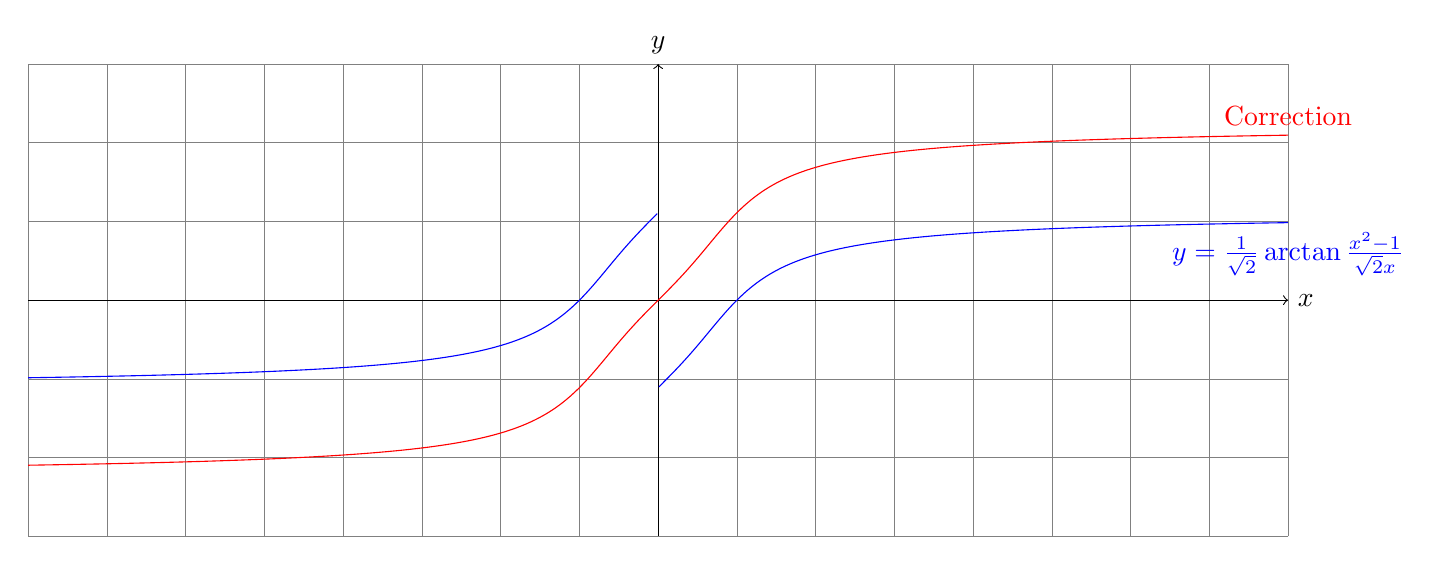
\begin{tikzpicture}[domain=-8:8]
\draw[very thin,color=gray](-8,-3)grid(8,3);
\draw[->](-8,0)--(8,0)node[right]{$x$};
\draw[->](0,-3)--(0,3)node[above]{$y$};
\draw[domain=-8:-0.01,samples=200,smooth,color=blue]plot(\x,{atan((\x*\x-1)/(sqrt(2)*\x))/180*pi/sqrt(2)});
\draw[domain=0.01:8,samples=200,smooth,color=blue]plot(\x,{atan((\x*\x-1)/(sqrt(2)*\x))/180*pi/sqrt(2)})node[below]{$y=\frac{1}{\sqrt{2}}\arctan{\frac{x^{2}-1}{\sqrt{2}x}}$};
\draw[samples=400,smooth,color=red]plot(\x,{(atan(1+sqrt(2)*\x)-atan(1-sqrt(2)*\x))/180*pi/sqrt(2)})node[above]{Correction};
\end{tikzpicture}
\end{center}\par
蓝色的图像是$C=0$的情况下描出来的函数图像, 而红色的是修正得到的完美图像. 可以看到, 蓝色的图像有一个跳跃间断点, 这个间断点也就是我们之前分子分母同除$x^{2}$的时候引入的间断点. 其实如果分正负区间来看呢, 每个区间上红色和蓝色图像都是平行的, 仅仅差个常数. \par
这个不定积分的结果对不对呢? 其实是对的. 但是如果直接拿来算定积分的话, 要小心踩雷啦. 
\begin{align*}
\int_{-1}^{1}\frac{x^{2}+1}{x^{4}+1}\dif{x}=\eval{\frac{1}{\sqrt{2}}\arctan{\frac{x^{2}-1}{\sqrt{2}x}}}_{-1}^{1}=0
.\end{align*}
像这样直接代入的话, 就会出错, 因为你求出来的那个原函数在$\left(-1,1\right)$不连续啊. 正确的做法就是分段积分, 像这样: 
\begin{align*}
\int_{-1}^{0}\frac{x^{2}+1}{x^{4}+1}\dif{x}+\int_{0}^{1}\frac{x^{2}+1}{x^{4}+1}\dif{x}=\frac{\pi}{\sqrt{2}}
.\end{align*}\par
所以总结一下, 恒等变换最严格的要求是定义域不能改变, 次严格的要求是只能引入有限个第一类间断点. 对于不定积分来说, 被积函数中引入有限个第一类间断点的变形是可以接受的, 但是无论如何不能把一部分区间的定义域给搞没了, 那就有问题了. \par
\subsection{绝对值与符号函数}
符号函数$\sgn{x}$的定义是
{
\setstretch{1.2}
\setlength{\parskip}{0.4em}
\begin{align*}
\sgn{x}=\begin{cases}
1&,x>0\\
0&,x=0\\
-1&,x<0
\end{cases}
.\end{align*}
}\par
这个函数在积分中的主要作用是加或者去绝对值符号, 而且符号函数可以当常数处理, 性质比较好. 符号函数加或去绝对值是依靠以下两个恒等式来进行的: 
\begin{align*}
\qty|x|=x\sgn{x}.\\
x=\qty|x|\sgn{x}
.\end{align*}
接下来我讲讲这方面的应用. \par
来看这道题: 
\begin{align*}
\int\qty|x|\dif{x}
.\end{align*}
这题我可以去绝对值符号了, 直接变形成
\begin{align*}
\int x\sgn{x}\dif{x}
.\end{align*}
接下来我们可以直接把$\sgn{x}$当作常数提到积分号以外了. 为什么能当成常数呢? 大家想啊, 当$x>0$的时候$\sgn{x}=1$吧, 那我可以把它提到积分号外; 当$x<0$的时候$\sgn{x}=-1$吧, 那我也可以把它提到积分号外. 这个效果就相当于什么呢, $x>0$的时候我把这个积分的系数写成$1$, 当$x<0$的时候我把这个积分的系数写成$-1$, 那不就相当于这个积分的系数是$\sgn{x}$了吗? \par
这个推导的逻辑链条我可以写成这样: 
\begin{align*}
\int f(x)\sgn{x}\dif{x}=\begin{cases}
\int f(x)\dif{x}&,x>0\\
\int -f(x)\dif{x}&,x<0
\end{cases}=\begin{cases}
\int f(x)\dif{x}&,x>0\\
-\int f(x)\dif{x}&,x<0
\end{cases}=\sgn{x}\int f(x)\dif{x}
.\end{align*}
于是回到原来的问题, 我们解这个积分: 
\begin{align*}
\int\qty|x|\dif{x}=\int x\sgn{x}\dif{x}=\sgn{x}\int x\dif{x}=\frac{x^{2}}{2}\sgn{x}+C
.\end{align*}
当然, 如果觉得这样写起来比较丑的话, 还可以化简一下形式, 写成$\frac{x\qty|x|}{2}+C$. \par
再来看一下这个积分: 
\begin{align*}
\int\sqrt[4]{x^{2}}\dif{x}
.\end{align*}
这个时候大家很有可能就会落入一个陷阱当中, 把被积函数化简成
\begin{align*}
\sqrt[4]{x^{2}}=\sqrt{x}
.\end{align*}
这样就犯了改变函数定义域的错误, 原来的定义域是$\mathbb{R}$, 现在变成了$\left[0,+\infty\right)$. 正确的做法是开偶数次根式的时候带上绝对值符号. 
\begin{align*}
\int\sqrt[4]{x^{2}}\dif{x}=\int\sqrt{\qty|x|}\dif{x}
.\end{align*}
这个绝对值符号就不容易去, 那么我们可以在其它的地方加绝对值符号, 从而统一积分变量. 
\begin{align*}
\int\sqrt{\qty|x|}\dif{x}=\sgn{x}\int\sqrt{\qty|x|}\dif{\qty|x|}
.\end{align*}
现在就变成了一个常规的幂函数积分. 
\begin{align*}
\sgn{x}\int\qty|x|^{\frac{1}{2}}\dif{\qty|x|}=\frac{2\qty|x|}{3}\sqrt{\qty|x|}\sgn{x}+C=\frac{2x}{3}\sqrt{\qty|x|}+C
.\end{align*}
开偶数次根号要带绝对值符号, 这种错误大家不会直接犯, 但是有些时候可能压根就没想到过. 比如说吧, 写$\ln{x^{2}}=2\ln{x}$这就不严谨了, 应该是$\ln{x^{2}}=2\ln\qty|x|$才对. 不过到目前为止我还没见过哪个老师从这么刁钻的角度挖坑. 一般大家做类似$\int x^{n}\ln^{m}{x^{l}}\dif{x}$的积分的时候也不会在意, 都默认$x>0$了. \par
这个时候你问我该咋办, 我也只能说, 猜出题老师的意图吧, 一般老师也想不到$\ln$里面开根号还有这回事. 考试的时候我也不会这么考你们的, 所以还是按照一般方法写吧. 但大家仍然要知道, 这个写法并不严谨. \par
\section{参数方程与有理化}
很多根式在平面直角坐标系里是有一定的几何意义的, 比如说
\begin{align*}
y=\sqrt{1-x^{2}}
.\end{align*}
它的几何意义就是一个圆$x^{2}+y^{2}=1$的上半部分, 你算一下就知道了. 再比如说
\begin{align*}
y=\sqrt{x+3}
.\end{align*}
它的几何意义就是一个抛物线$y^{2}=x+3$的上半部分, 也不难理解. \par
现在我们遇到了一个这样的问题: 被积函数里有一个根式, 我们要想办法消根号. 于是我们开始思考, 我们可以通过适当的参数方程来实现这个目的. 如果能变出一个$\sqrt{u^{2}}$的结构来, 那么自然就消掉了根号, 变成有理函数积分了. \par
啊, 你们高中没学过参数方程啊? 已经不讲了啊? 不早说! 那我先简单介绍一下参数方程啊, 可能会导致拖课. \par
\subsection{参数方程简介}
很多时候我们拿到一个曲线方程的时候, 是需要把它化成显函数来处理的, 举个例子, 比如对曲线
\begin{align*}
x^{2}+y=1
,\end{align*}
要求积分$\int y\dif{x}$. 我们的常规思路是要统一变量对吧, 那么我就把$y$写成关于$x$的形式, 也就是对原来的曲线方程做一个变换: 
\begin{align*}
y={}&1-x^{2}
.\end{align*}
这样之后再将$y$关于$x$的函数代入到原来的积分当中去做. \par
有些曲线容易显化为$x$关于$y$的函数, 比如说
\begin{align*}
x-y=y^{5}+1
.\end{align*}
这个很难显化成$y$关于$x$的函数, 就算做到了也会很难看. 于是我们统一变量$y$来进行积分. 
\begin{align*}
\int y\dif{x}=xy-\int x\dif{y}=xy-\int\qty(y^{5}+y+1)\dif{y}
.\end{align*}
这儿还用到了分部积分, 也是个很常见的操作. \par
现在有些曲线, 既不容易显化为$y$关于$x$的函数, 也不容易显化为$x$关于$y$的函数, 这样一来混合着$x$和$y$的积分就不太好处理了. 比如说这个: 
\begin{align*}
y\qty(x-y)^{2}=x
.\end{align*}
这玩意儿你要是用解方程的法子硬做的话, 最后会整理出非常丑陋的形式, 有兴趣的同学可以试试. \par
现在我们遇到了困难, 混合着$x$和$y$的积分很难统一变量成$x$或者$y$, 这个时候我们就应该引入一个新的变量$t$来帮我们解围. 这个新的变量应该满足两个条件: \par
第一, 无论$x$还是$y$都能用关于$t$的函数来表示, 换句话说$t$是来帮我们对$x$和$y$分别进行显化的. \par
第二, 在$t$取任何合理值的时候, $x$和$y$的值要使曲线方程依旧成立. \par
这个时候我们就把$t$当作是参数, 而$x$和$y$都表达成关于$t$的函数, 这两个函数联立一下, 就构成了我们需要的参数方程. 这么讲比较抽象, 我拿一个椭圆来开个刀吧: 
\begin{align*}
3x^{2}+4y^{2}=12
.\end{align*}\par
我们需要选取两个尽可能简单的函数$x(t),\,y(t)$, 使得这个椭圆方程仍然是成立的. 考虑到这是个平方和为常数的结构, 我们可以选用正余弦函数. 
\begin{align*}
\begin{cases}
x=2\cos{t}\\
y=\sqrt{3}\sin{t}
\end{cases}
.\end{align*}
再来确定一下定义域, 也就是$t$的取值范围. 这个取值范围没啥特别的要求, $t\in\mathbb{R}$就行. 当然如果你愿意, 也可以设置一个比较严格的定义域, 比如$t\in\left[0,2\pi\right)$. \par
最后把这个参数方程代回原方程去看一下. 
\begin{align*}
3(2\cos{t})^{2}+4(\sqrt{3}\sin{t})^{2}=12\cos^{2}{t}+12\sin^{2}{t}=12
.\end{align*}
原来的方程能成立, 那就没问题了. \par
参数方程是怎么把一条曲线给画出来的呢? 咱们可以类比联想一下我们画函数图像时候的操作, 我们选定几个$x$, 然后确定对应的$y(x)$值, 接着在图上描出这几个$\qty(x,y)$点, 最后连成一条光滑的曲线, 就是我们需要的函数图像了. \par
那么用参数方程来画曲线的时候, 我们也是这样的. 先选定几个$t$, 然后确定对应的$x(t)$和$y(t)$值, 接着在图上描出这几个$\qty(x,y)$点, 最后连成一条光滑的曲线. \par
好了, 参数方程我就介绍到这里. 时间紧迫, 我快点讲, 大家能早点下课. \par
\subsection{含$\sqrt[n]{ax+b}$的情形}
来思考一下这样一个问题, 现在被积函数当中出现了$y=\sqrt[n]{ax+b}$的结构, 要怎么处理? 典型的例题是下面这几个: 
\begin{align*}
\int\frac{\dif{x}}{\sqrt[4]{x+1}},\,\int\frac{\dif{x}}{\sqrt{x}+\sqrt{1-x}},\,\int\frac{1-\sqrt{x}}{1+\sqrt[3]{x}}\dif{x}
.\end{align*}
我们就用参数方程的知识来思考一下这些问题的有理化方法. \par
先看看积分$\int\frac{\dif{x}}{\sqrt[4]{x+1}}$. 在这里出现的根式只有一个: $y=\sqrt[4]{x+1}$. 我们发现这个方程很容易显化成$x$关于$y$的有理函数: 
\begin{align*}
y={}&\sqrt[4]{x+1}\\
y^{4}={}&x+1\\
x={}&y^{4}-1
.\end{align*}
所以我们只需要在原来的积分中把所有的$x$都换成关于$y$的函数就行了, 我写一下: 
\begin{align*}
\int\frac{\dif{x}}{\sqrt[4]{x+1}}=\int\frac{\dif{\qty(y^{4}-1)}}{\sqrt[4]{y^{4}}}
.\end{align*}
现在问大家一个问题, 开根式$\sqrt[4]{y^{4}}$用不用套绝对值? 是不需要的, 因为前面的关系式$y=\sqrt[4]{x+1}$以及$y$在分母上都说明$y>0$. 所以直接开根式得到$y$就行. 
\begin{align*}
\int\frac{\dif{y^{4}}}{y}=4\int y^{2}\dif{y}=\frac{4}{3}y^{3}+C
.\end{align*}
最后只需要用$y=\sqrt[4]{x+1}$回代一下就行了. \par
对于奇数次根式也是同理的, 比如说$\int\frac{\dif{x}}{1+\sqrt[3]{x-1}}$吧, 这当中出现的根式只有$y=\sqrt[3]{x-1}$, 而这个很容易显化成$x$关于$y$的有理函数$x=y^{3}+1$, 所以
\begin{align*}
\int\frac{\dif{x}}{1+\sqrt[3]{x-1}}=\int\frac{\dif{y^{3}}}{1+\sqrt[3]{y^{3}}}=3\int\frac{y^{2}\dif{y}}{y+1}
.\end{align*}\par
再来看积分$\int\frac{\dif{x}}{\sqrt{x}+\sqrt{1-x}}$. 这个积分的难点在哪儿呢, 分母上是两个根式的和, 看起来就很难处理. 我们要想办法让它尽量容易做, 最好能把两个根式分而治之, 所以我们选择先用平方差公式后分项. 
\begin{align*}
\int\frac{\dif{x}}{\sqrt{x}+\sqrt{1-x}}=\int\frac{\sqrt{x}-\sqrt{1-x}}{x-\qty(1-x)}\dif{x}=\int\frac{\sqrt{x}\dif{x}}{2x-1}-\int\frac{\sqrt{1-x}\dif{x}}{2x-1}
.\end{align*}
这样有个什么好处呢, 分母有理化了之后根式全都在分子上, 而分子是可以任意分项的, 于是我们就把两个根式分开放到两个积分里, 现在我们只需要分别解决这两个积分就行了. 先看第一个. 这里有根式$y=\sqrt{x}$, 这个很容易显化成$x$关于$y$的有理函数$x=y^{2}$, 所以
\begin{align*}
\int\frac{\sqrt{x}\dif{x}}{2x-1}=\int\frac{y\dif{y^{2}}}{2y^{2}-1}=2\int\frac{y^{2}\dif{y}}{2y^{2}-1}
.\end{align*}
再看第二个. 这里有根式$z=\sqrt{1-x}$, 也很容易显化成$x$关于$z$的有理函数$x=1-z^{2}$, 所以
\begin{align*}
\int\frac{\sqrt{1-x}\dif{x}}{2x-1}-\int\frac{z\dif{\qty(-z^{2})}}{2-2z^{2}-1}=2\int\frac{z^{2}\dif{z}}{2z^{2}-1}
.\end{align*}
两个积分都求出来之后, 分别回代化成关于$x$的形式就可以了. \par
最后来看积分$\int\frac{1-\sqrt{x}}{1+\sqrt[3]{x}}\dif{x}$. 如果你想用立方和公式把分母有理化的话, 能做倒是能做, 但太复杂了. 还是那句话, 适用范围广的做法未必就快. 这题最快的方式是换元$x=t^{6}$并规定$t\in\left[0,+\infty\right)$, 能直接把两个根号都消掉, 把原来的积分变成有理函数积分. 
\begin{align*}
\int\frac{1-\sqrt{x}}{1+\sqrt[3]{x}}\dif{x}=\int\frac{1-t^{3}}{1+t^{2}}\dif{t^{6}}=6\int\frac{t^{5}-t^{8}}{t^{2}+1}\dif{t}
.\end{align*}
顺便一说, 用参数方程的话要把参数的取值范围规定好, 一般能规定个小点的区间就不要规定太大的, 这点我们后面讲三角函数的时候会说. \par
\subsection{针对$\sqrt{ax^{2}+bx+c}$的三角/双曲换元}
现在我们来考虑这样一种积分, 被积函数中含有$y=\sqrt{ax^{2}+bx+c}$的结构. 为了研究方便呢, 我们先来考虑这三种简单情形, 分别是$\sqrt{1-x^{2}},\,\sqrt{x^{2}+1},\,\sqrt{x^{2}-1}$, 然后再推广到一般情形. \par
当被积函数中含有根式$y=\sqrt{1-x^{2}}$的时候, 它是个圆, 我们可以使用参数方程
\begin{align*}
\begin{cases}
x=\sin{t}\\
y=\cos{t}
\end{cases}
\end{align*}
来实现有理化. 我们思考一下$t$的取值范围吧, 要尽可能小, 但必须让$\sin{t}$涵盖$x$的所有取值. 考虑到$x,y$的范围分别是$x\in\left[-1,1\right],\,y\in\left[0,1\right]$, 所以我们将$t$的范围定为$t\in\left[-\frac{\pi}{2},\frac{\pi}{2}\right]$. \par
接下来我们就可以在类似的问题中进行代换了, 比如说
\begin{align*}
\int\frac{\dif{x}}{1+\sqrt{1-x^{2}}}=\int\frac{\dif{\sin{t}}}{1+\cos{t}}=\int\frac{\cos{t}\dif{t}}{1+\cos{t}}
.\end{align*}
这样我们就把原来的无理函数积分变成了一个三角有理式的积分, 三角有理式积分就可做了. 上面这题解出来原函数
\begin{align*}
t+\cot{t}-\csc{t}+C
.\end{align*}
这还没完, 我们要把关于$t$的式子变回关于$x$的式子才行. \par
首先我们根据$x=\sin{t},\,t\in\left[-\frac{\pi}{2},\frac{\pi}{2}\right]$可以知道$t=\arcsin{x}$. 这也就是我们要把$t$限制在区间$\left[-\frac{\pi}{2},\frac{\pi}{2}\right]$里的原因, 如果$t$可以取到$\left[k\pi-\frac{\pi}{2},k\pi+\frac{\pi}{2}\right]\qty(k\in\mathbb{Z})$的话, 这个反函数就要写成$t=\arcsin{x}+k\pi$的形式, 这么搞没啥必要. \par
接下来处理$\cot{t}-\csc{t}$, 我们有两种方式. 第一种是通过恒等变换, 把这个式子用$\sin{t}$和$\cos{t}$的有理式来表达, 最后直接通过参数方程回代, 我写一下. 
\begin{align*}
t+\cot{t}-\csc{t}+C={}&\arcsin{x}+\frac{\cos{t}}{\sin{t}}-\frac{1}{\sin{t}}+C\\
={}&\arcsin{x}+\frac{\sqrt{1-x^{2}}}{x}-\frac{1}{x}+C
.\end{align*}\par
第二种方法是画辅助三角形, 辅助三角形画出来之后六个三角函数的回代表达式都能很直观地看出来. \\
\begin{center}
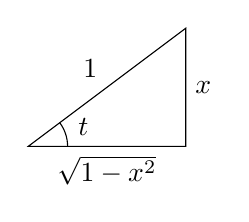
\begin{tikzpicture}
\draw (0,0)--node[below]{$\sqrt{1-x^{2}}$}(2,0)--node[right]{$x$}(2,1.5)--node[above left]{$1$}cycle;
\draw (0.5,0)arc(0:37:0.5);
\draw node at(0.7,0.25){$t$};
\end{tikzpicture}
\end{center}\par
我们画一个直角三角形, 设其中一个锐角为$t$, 然后根据边角关系$x=\sin{t},\,\sqrt{1-x^{2}}=\cos{t}$将三个边都设出来. 接下来我们根据这个辅助三角形就可以直接写出$t$的六个三角函数用$x$表达的形式了: 
\begin{align*}
\sin{t}=x,\;\cos{t}=\sqrt{1-x^{2}},\;\tan{t}=\frac{x}{\sqrt{1-x^{2}}},\\
\csc{t}=\frac{1}{x},\;\sec{t}=\frac{1}{\sqrt{1-x^{2}}},\;\cot{t}=\frac{\sqrt{1-x^{2}}}{x}
.\end{align*}
于是我们直接回代得到
\begin{align*}
t+\cot{t}-\csc{t}+C=\arcsin{x}+\frac{\sqrt{1-x^{2}}}{x}-\frac{1}{x}+C
.\end{align*}
再来看$y=\sqrt{x^{2}+1}$的形式, 这是焦点位于$y$轴上的双曲线的上一支. 在这里我们可以使用参数方程
\begin{align*}
\begin{cases}
x=\tan{t}\\
y=\sec{t}
\end{cases}
\end{align*}
来实现有理化. 我们思考一下$t$的取值范围, 定为$\left(-\frac{\pi}{2},\frac{\pi}{2}\right)$是最合理的. \par
拿道例题来说吧, 
\begin{align*}
\int\frac{\dif{x}}{\sqrt{x^{2}+1}}=\int\frac{\dif{\tan{t}}}{\sec{t}}=\int\sec{t}\dif{t}=\ln(\sec{t}+\tan{t})+C=\ln(x+\sqrt{x^{2}+1})+C
.\end{align*}
这个题比较特殊, 我们可以直接用套用参数方程来回代, 不需要画辅助三角形了. 但是我也画一个, 因为在其它题目里可能就用着了. 
\begin{center}
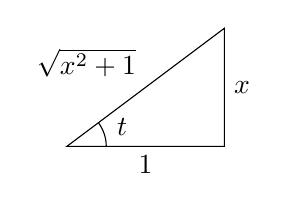
\begin{tikzpicture}
\draw (0,0)--node[below]{$1$}(2,0)--node[right]{$x$}(2,1.5)--node[above left]{$\sqrt{x^{2}+1}$}cycle;
\draw (0.5,0)arc(0:37:0.5);
\draw node at(0.7,0.25){$t$};
\end{tikzpicture}
\end{center}
于是得到
\begin{align*}
\sin{t}=\frac{x}{\sqrt{x^{2}+1}},\;\cos{t}=\frac{1}{\sqrt{x^{2}+1}},\;\tan{t}=x,\\
\csc{t}=\frac{\sqrt{x^{2}+1}}{x},\;\sec{t}=\sqrt{x^{2}+1},\;\cot{t}=\frac{1}{x}
.\end{align*}\par
最后来看$y=\sqrt{x^{2}-1}$的形式, 这是焦点位于$x$轴上的双曲线在$x$轴上方的部分. 在这里我们需要分区间来使用参数方程. 在$x\in\left[1,+\infty\right)$的时候我们使用参数方程
\begin{align*}
\begin{cases}
x=\sec{t}\\
y=\tan{t}
\end{cases}
\end{align*}
来实现有理化, 其中$t$的取值范围定为$\left[0,\frac{\pi}{2}\right)$. 而在$x\in\left(-\infty,-1\right]$的时候我们使用参数方程
\begin{align*}
\begin{cases}
x=\sec{t}\\
y=-\tan{t}
\end{cases}
\end{align*}
来实现有理化, 其中$t$的取值范围定为$\left(\frac{\pi}{2},\pi\right)$. 这里大家可以自行代入验证. 时间紧张, 我直接上例题.  当$x\ge1$的时候, 
\begin{align*}
\int\frac{\dif{x}}{\sqrt{x^{2}-1}}=\int\frac{\dif{\sec{t}}}{\tan{t}}=\int\sec{t}\dif{t}=\ln\qty|\sec{t}+\tan{t}|+C=\ln\qty|x+\sqrt{x^{2}-1}|+C
.\end{align*}
而当$x\le-1$的时候
\begin{align*}
\int\frac{\dif{x}}{\sqrt{x^{2}-1}}=\int\frac{\dif{\sec{t}}}{-\tan{t}}=-\int\sec{t}\dif{t}=-\ln\qty|\sec{t}+\tan{t}|+C=-\ln\qty|x-\sqrt{x^{2}-1}|+C
.\end{align*}\par
这个参数方程对应的辅助三角形长什么样呢, 也是需要分类讨论的. 当$x\ge1$的时候它长这样: 
\begin{center}
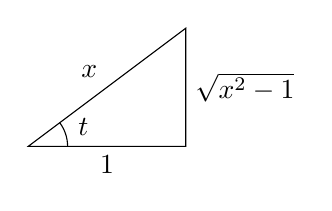
\begin{tikzpicture}
\draw (0,0)--node[below]{$1$}(2,0)--node[right]{$\sqrt{x^{2}-1}$}(2,1.5)--node[above left]{$x$}cycle;
\draw (0.5,0)arc(0:37:0.5);
\draw node at(0.7,0.25){$t$};
\end{tikzpicture}
\end{center}
于是得到
\begin{align*}
\sin{t}=\frac{\sqrt{x^{2}-1}}{x},\;\cos{t}=\frac{1}{x},\;\tan{t}=\sqrt{x^{2}-1},\\
\csc{t}=\frac{x}{\sqrt{x^{2}-1}},\;\sec{t}=x,\;\cot{t}=\frac{1}{\sqrt{x^{2}-1}}
.\end{align*}
而当$x\le-1$的时候它就长这样了: 
\begin{center}
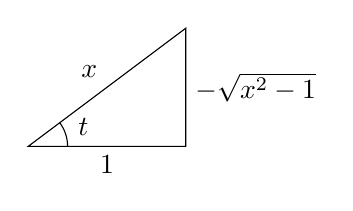
\begin{tikzpicture}
\draw (0,0)--node[below]{$1$}(2,0)--node[right]{$-\sqrt{x^{2}-1}$}(2,1.5)--node[above left]{$x$}cycle;
\draw (0.5,0)arc(0:37:0.5);
\draw node at(0.7,0.25){$t$};
\end{tikzpicture}
\end{center}
于是得到
\begin{align*}
\sin{t}=-\frac{\sqrt{x^{2}-1}}{x},\;\cos{t}=\frac{1}{x},\;\tan{t}=-\sqrt{x^{2}-1},\\
\csc{t}=-\frac{x}{\sqrt{x^{2}-1}},\;\sec{t}=x\:,\;\cot{t}=-\frac{1}{\sqrt{x^{2}-1}}
.\end{align*}\par
其实积分$\int\frac{\dif{x}}{\sqrt{x^{2}-1}}$虽然经过了分类讨论化成不同的形式, 但它们可以统一成单一的形式. 因为
\begin{align*}
-\ln\qty|x-\sqrt{x^{2}-1}|=\ln\qty|\frac{1}{x-\sqrt{x^{2}-1}}|=\ln\qty|\frac{x+\sqrt{x^{2}-1}}{x^{2}-x^{2}+1}|=\ln\qty|x+\sqrt{x^{2}-1}|
.\end{align*}
所以我们整理一下结果: 
\begin{align*}
\int\frac{\dif{x}}{\sqrt{x^{2}-1}}=\ln\qty|x+\sqrt{x^{2}-1}|+C
.\end{align*}
三角换元我们简单讲过了, 接下来粗略介绍一下双曲换元吧. 双曲函数可以作为双曲线的参数方程, 比如说对于$y=\sqrt{x^{2}+1}$来说, 我们可以用参数方程
\begin{align*}
\begin{cases}
x=\sinh{t}\\
u=\cosh{t}
\end{cases}
\end{align*}
来实现有理化, 其中$t$的取值范围是$\left(-\infty,+\infty\right)$. 拿道例题来说吧: 
\begin{align*}
\int\frac{\dif{x}}{\sqrt{x^{2}+1}}=\int\frac{\dif{\sinh{t}}}{\cosh{t}}=t+C=\arsinh{t}+C
.\end{align*}
同样的道理, 对于$y=\sqrt{x^{2}-1}$来索, 我们也可以使用参数方程. 不过这里要分区间考虑. 我们在区间$x\in\left[1,+\infty\right)$上使用参数方程
\begin{align*}
\begin{cases}
x=\cosh{t}\\
y=\sinh{t}
\end{cases}
,\end{align*}
而在区间$x\in\left(-\infty,1\right]$上使用参数方程
\begin{align*}
\begin{cases}
x=-\cosh{t}\\
y=\sinh{t}
\end{cases}
.\end{align*}
一看就很麻烦对吧. 还有更麻烦的, 那就是你不能画辅助图形来快速判断$\tanh{t},\,\coth{t},\,\sech{t},\,\csch{t}$的表达式, 这是很致命的. 也正因为这些原因, 我们是不推荐使用双曲换元的, 所以这里仅仅做个介绍. \par
说回三角换元. 现在我们已经能够解决$\sqrt{1-x^{2}},\,\sqrt{x^{2}+1},\,\sqrt{x^{2}-1}$这三类问题了, 那么我们就来适当推广一下吧: 
\begin{align*}
\int\frac{\dif{x}}{\sqrt{a^{2}-x^{2}}}\;\qty(a>0),\,\int\sqrt{x^{2}+2x+2}\dif{x},\,\int\frac{\dif{x}}{\sqrt{4x^{2}-4x-1}}
.\end{align*}
这三个问题也是可以用三角换元来操作的, 不过看上去好像比较麻烦, 我来讲一讲. \par
先看$\int\frac{\dif{x}}{\sqrt{a^{2}-x^{2}}}$, 这里我们可以换元$x=a\sin{t}$, 并限制$t\in\left[-\frac{\pi}{2},\frac{\pi}{2}\right]$, 于是
\begin{align*}
\sqrt{a^{2}-x^{2}}=\sqrt{a^{2}\qty(1-\sin^{2}{x})}=a\sqrt{\cos^{2}{t}}=a\cos{t}
.\end{align*}
大家要注意, 因为在区间$t\in\left[-\frac{\pi}{2},\frac{\pi}{2}\right]$当中恒有$\cos{t}\ge0$, 所以开根号不需要带绝对值了. 所以
\begin{align*}
\int\frac{\dif{x}}{\sqrt{a^{2}-x^{2}}}=\int\frac{\dif{\qty(a\sin{t})}}{a\cos{t}}=\int\dif{t}=t+C
.\end{align*}
最后一步是回代, 可以画辅助三角形, 不过没必要. 
\begin{align*}
\frac{x}{a}={}&\sin{t}\\
t={}&\arcsin{\frac{x}{a}}
.\end{align*}
所以原来的积分就解出来了. 
\begin{align*}
\int\frac{\dif{x}}{\sqrt{a^{2}-x^{2}}}=\arcsin{\frac{x}{a}}+C.\qty(a>0)
\end{align*}
接下来看$\int\sqrt{x^{2}+2x+2}\dif{x}$, 这里我们的思路是先配方, 然后整体换元. 
\begin{align*}
\int\sqrt{\qty(x+1)^{2}+1}\dif{x}
.\end{align*}
所以这里只需要换元$x+1=\tan{t}$, 并限制$t\in\left(-\frac{\pi}{2},\frac{\pi}{2}\right)$, 于是
\begin{align*}
\sqrt{\qty(x+1)^{2}+1}=\sqrt{\tan^{2}{t}+1}=\sqrt{\sec^{2}{t}}=\sec{t}
.\end{align*}
大家要注意, 因为在区间$t\in\left(-\frac{\pi}{2},\frac{\pi}{2}\right)$中恒有$\sec{t}>0$, 所以开根号不用带绝对值了. 所以
\begin{align*}
\int\sqrt{x^{2}+2x+2}\dif{x}=\int\sec{t}\dif{\tan{t}}=\int\sec^{3}{t}\dif{t}
.\end{align*}
这是我们都很熟悉的积分, 我就不多说了. 这里我只管把辅助三角形画一下. 
\begin{center}
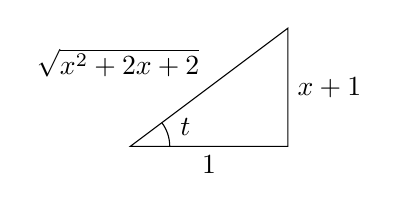
\begin{tikzpicture}
\draw (0,0)--node[below]{$1$}(2,0)--node[right]{$x+1$}(2,1.5)--node[above left]{$\sqrt{x^{2}+2x+2}$}cycle;
\draw (0.5,0)arc(0:37:0.5);
\draw node at(0.7,0.25){$t$};
\end{tikzpicture}
\end{center}
这样就得到
\begin{align*}
\sin{t}=\frac{x+1}{\sqrt{x^{2}+2x+2}},\;\cos{t}=\frac{1}{\sqrt{x^{2}+2x+2}},\;\tan{t}=x+1,\\
\csc{t}=\frac{\sqrt{x^{2}+2x+2}}{x+1},\;\sec{t}=\sqrt{x^{2}+2x+2},\;\cot{t}=\frac{1}{x+1}
.\end{align*}\par
最后看$\int\frac{\dif{x}}{\sqrt{4x^{2}-4x-1}}$, 我们依然是在这个根式内部进行配方, 最后依据配方情况使用适当的三角换元. 
\begin{align*}
\int\frac{\dif{x}}{\sqrt{\qty(2x-1)^{2}-2}}
.\end{align*}
于是我们换元$2x-1=\sqrt{2}\sec{t}$, 并限制$t\in\left[0,\frac{\pi}{2}\right)\cup\left(\frac{\pi}{2},\pi\right)$, 于是
\begin{align*}
\sqrt{\qty(2x-1)^{2}-2}=\sqrt{2\tan^{2}{t}}=\begin{cases}
\sqrt{2}\tan{t}&,t\in\left[0,\frac{\pi}{2}\right)\\
-\sqrt{2}\tan{t}&,t\in\left(\frac{\pi}{2},\pi\right)
\end{cases}
.\end{align*}
接下来就是分区间讨论积分结果了, 这个操作真的很无聊哎, 要不留给你们当作业吧? \par
行, 没有同学反对, 那我们抓紧时间讲欧拉换元. \par
\subsection{针对$\sqrt{ax^{2}+bx+c}$的欧拉换元}
我们之前提到过函数$y=\sqrt{ax^{2}+bx+c}$所代表的几何意义是二次曲线. 我们可以根据参数的取值情况将曲线的类型细分一下. 注意, 这里探讨的范围都是实数域, 咱不考虑复数域. \par
当$a=0$时, 这玩意儿就是一个抛物线$y^{2}=bx+c$在$x$轴上方的部分. 这个东西其实就用不着欧拉换元了, 我们之前讲的方法已经足够对付了. \par
当$a>0$并且$b^{2}-4ac\ne0$时, 这玩意儿就是一个双曲线. 为什么这里还要考虑$\Delta=b^{2}-4ac$呢, 因为当$\Delta=0$的时候这个根号里面一配方就直接开出来了, 变成绝对值函数了, 那就不算双曲线了. \par
如果进一步细分$a>0$情况下$\Delta$的取值的话, 我们还可以得到更详细的结论. 当$\Delta<0$的时候, 这个曲线和$x$轴是没有交点的, 完整的曲线应该是焦点连线平行于$y$轴的; 当$\Delta>0$的时候, 这个曲线和$x$轴是有交点的, 完整的曲线焦点就在$x$轴上. \par
为了直观, 我在这儿画两个函数图像. 蓝色的是$\Delta<0$的情况, 与$x$轴没有交点; 红色的是$\Delta>0$的情况, 与$x$轴有交点. 原本的曲线只有$x$轴以上的部分, 而$x$轴以下的部分我给用虚线补齐了. 
\begin{center}
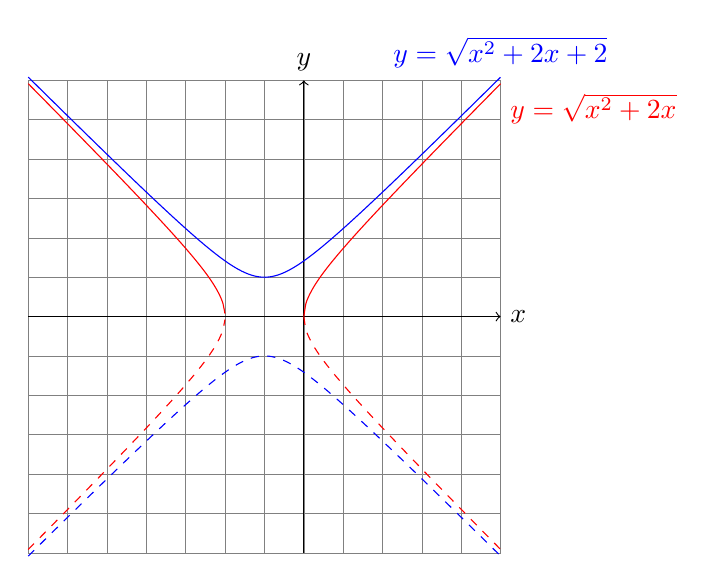
\begin{tikzpicture}[domain=-3.5:2.5]
\draw[step=0.5,very thin,color=gray](-3.5,-3)grid(2.5,3);
\draw[->](-3.5,0)--(2.5,0)node[right]{$x$};
\draw[->](0,-3)--(0,3)node[above]{$y$};
\draw[domain=-3.5:2.5,samples=200,smooth,color=blue]plot(\x,{sqrt((\x*2+1)*(\x*2+1)+1)/2})node[above]{$y=\sqrt{x^{2}+2x+2}$};
\draw[dashed,domain=-3.5:2.5,samples=200,smooth,color=blue]plot(\x,{-sqrt((\x*2+1)*(\x*2+1)+1)/2});
\draw[domain=-3.5:-1,samples=100,smooth,color=red]plot(\x,{sqrt((\x*2+1)*(\x*2+1)-1)/2});
\draw[domain=0:2.5,samples=100,smooth,color=red]plot(\x,{sqrt((\x*2+1)*(\x*2+1)-1)/2})node[below right]{$y=\sqrt{x^{2}+2x}$};
\draw[dashed,domain=-3.5:-1,samples=100,smooth,color=red]plot(\x,{-sqrt((\x*2+1)*(\x*2+1)-1)/2});
\draw[dashed,domain=0:2.5,samples=100,smooth,color=red]plot(\x,{-sqrt((\x*2+1)*(\x*2+1)-1)/2});
\end{tikzpicture}
\end{center}\par
当$a<0$的时候呢, 我们只需要考虑$\Delta>0$的情况. 这是因为当$a<0$且$\Delta<0$的时候, 一定有$ax^{2}+bx+c<0$, 套上根号之后发现定义域没了, 这个函数图像就没意义了. 同样的道理, 当$a<0$且$\Delta=0$的时候, 根式$\sqrt{ax^{2}+bx+c}$也只在一个点上有定义, 没必要去考虑相关的积分了. \par
当$a<0$并且$\Delta>0$的时候, 这个函数图像是一个圆或椭圆的一部分. 这里我们没有必要去进一步分析它的形状了, 我画两个图大家看一下就行了. 
\begin{center}
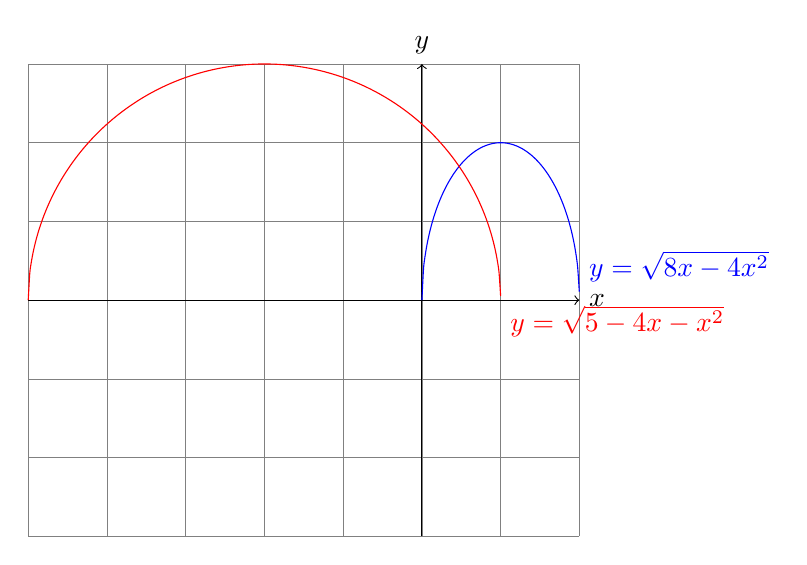
\begin{tikzpicture}
\draw[very thin,color=gray](-5,-3)grid(2,3);
\draw[->](-5,0)--(2,0)node[right]{$x$};
\draw[->](0,-3)--(0,3)node[above]{$y$};
\draw[domain=0:2,samples=100,smooth,color=blue]plot(\x,{sqrt(8*\x-4*\x*\x)})node[above right]{$y=\sqrt{8x-4x^{2}}$};
\draw[domain=-5:1,samples=300,smooth,color=red]plot(\x,{sqrt(5-4*\x-\x*\x)})node[below right]{$y=\sqrt{5-4x-x^{2}}$};
\end{tikzpicture}
\end{center}\par
搞懂$y=\sqrt{ax^{2}+bx+c}$的几何意义之后呢, 我们来正式开始讲解欧拉换元. 大家想啊, 高中学过的解析几何知识告诉我们, 任意一条直线和二次曲线最多只能有两个交点. 我可以事先定下一个交点$\qty(x_{0},\sqrt{ax_{0}^{2}+bx_{0}+c})$, 然后用直线的斜率$t$作为参数, 去画一条直线
\begin{align*}
l:\;y=t\qty(x-x_{0})+\sqrt{ax_{0}^{2}+bx_{0}+c}
.\end{align*}
不考虑$\qty(x_{0},\sqrt{ax_{0}^{2}+bx_{0}+c})$这个点的话呢, 直线$l$最多还能够确定二次曲线上的一个点$\qty(x,y)$. 而且这个点只和$t$有关, 因为其它的信息都是定好了的, 只有$t$是可变的参数. 换句话说, $x$和$y$都是可以用关于$t$的函数来表示的, 倘若这两个关于$t$的函数都是有理函数, 那么像$\int y\dif{x}$这类的积分不就变成有理函数积分了吗? \par
那么咱先来选一个点吧. 选点这事儿要讲究, 不能将就. 你要是随随便便就选一个点开始做, 那会很麻烦. 你那个直线方程都能写一大串呢. 我们来根据$a,\,b,\,c$的取值情况分两种取点方式. 
当$c>0$的时候, 曲线$y=\sqrt{ax^{2}+bx+c}$和$y$轴有交点$\qty(0,\sqrt{c})$. 这个时候我们可以写一个比较简洁的直线方程
\begin{align*}
y=tx+\sqrt{c}
.\end{align*}
接下来把这个方程和$y=\sqrt{ax^{2}+bx+c}$联立, 得到
\begin{align*}
\qty(k^{2}-a)x^{2}=\qty(b-2\sqrt{c}t)x
.\end{align*}
我们能够直接解出这个方程的根, 其中一个是$0$, 我们不管了; 另一个就是我们要求的$x$. 然后我们再通过直线方程把$y$也表示出来, 就能得到一个参数方程
\begin{align*}
\begin{cases}
x=\frac{b-2\sqrt{c}t}{t^{2}-a}\\
y=\frac{-\sqrt{c}t^{2}+bt-a\sqrt{c}}{t^{2}-a}
\end{cases}
.\end{align*}
这样, 当遇到$c>0$情况的时候, 就可以求出这个参数方程并套用了. \par
当$\Delta>0$的时候, 曲线$y=\sqrt{ax^{2}+bx+c}$无论是双曲线还是圆或椭圆, 都与$x$轴有两个交点$x_{1},\,x_{2}$. 于是我也可以把这个曲线改写成$y=\sqrt{a\qty(x-x_{1})\qty(x-x_{2})}$. 这种情况下我们可以选择其中的一个交点, 比如$\qty(x_{1},0)$, 写一个比较简洁的直线方程
\begin{align*}
y=t\qty(x-x_{1})
.\end{align*}
接下来把这个方程和$y=\sqrt{a\qty(x-x_{1})\qty(x-x_{2})}$联立, 就能解出$x$了, 代入到直线方程当中还能解出$y$, 所以参数方程就有了. 
\begin{align*}
\begin{cases}
x=\frac{t^{2}x_{1}-ax_{2}}{t^{2}-a}\\
y=\frac{ta\qty(x_{1}-x_{2})}{t^{2}-a}
\end{cases}
.\end{align*}\par
接下来还有另一种欧拉换元方式. 当$a>0$的时候, 这个图像是双曲线的一部分. 这个双曲线的渐近线方程是$\pm y=\sqrt{a}x+\frac{b}{2\sqrt{a}}$. 解析几何知识告诉我们, 与双曲线渐近线平行的直线和双曲线之间至多有一个交点. 	那么我可以设一条与双曲线平行的直线, 将纵截距$t$作为参数, 只要改变$t$就能够确定最多一个点$\qty(x,y)$. 比如说吧, 我就设直线方程
\begin{align*}
y=\sqrt{a}x+t
.\end{align*}
接下来把这个方程和$y=\sqrt{ax^{2}+bx+c}$联立, 就能解出$x$了, 再代入直线方程解出$y$, 就能得到参数方程
\begin{align*}
\begin{cases}
x=\frac{c-t^{2}}{2\sqrt{a}t-b}\\
y=\frac{\sqrt{a}t^{2}-bt+\sqrt{a}c}{2\sqrt{a}t-b}
\end{cases}
.\end{align*}\par
好了, 关于欧拉换元基本方法的介绍就到这里, 最后来说一下我对这个方法的评价吧. 欧拉换元作为一种有理化的方法, 它的计算量实在太大了, 平常我们是不推荐使用的. 我们可以拿一道例题来说明一下: 
\begin{align*}
\int\frac{\dif{x}}{x+\sqrt{x^{2}-5x+6}}
.\end{align*}
这里我先使用欧拉换元的方式, 设直线方程$y=t\qty(x-2)$然后将其与$y=\sqrt{x^{2}-5x+6}$联立. 解出参数方程
\begin{align*}
\begin{cases}
x=\frac{2t^{2}-3}{t^{2}-1}\\
y=-\frac{t}{t^{2}-1}
\end{cases}
.\end{align*}
于是原积分化成
\begin{align*}
\int\frac{\dif{\frac{2t^{2}-3}{t^{2}-1}}}{\frac{2t^{2}-3}{t^{2}-1}-\frac{t}{t^{2}-1}}={}&\int\frac{2t\dif{t}}{\qty(t-1)\qty(t+1)^{2}\qty(2t-3)}\\
={}&\frac{1}{5\qty(t+1)}+\frac{12}{25}\ln\qty|3-2t|-\frac{1}{2}\ln\qty|1-t|+\frac{1}{50}\ln\qty|t+1|+C
.\end{align*}
最后用$t=\frac{\sqrt{x^{2}-5x+6}}{x-2}$回代一下, 就得出原函数了. 
\begin{align*}
{}&\frac{x-2}{5\qty(\sqrt{x^{2}-5x+6}+x-2)}+\frac{12}{25}\ln\qty|3-\frac{2\sqrt{x^{2}-5x+6}}{x-2}|\\
{}&-\frac{1}{2}\ln\qty|1-\frac{\sqrt{x^{2}-5x+6}}{x-2}|+\frac{1}{50}\ln\qty|\frac{\sqrt{x^{2}-5x+6}}{x-2}+1|+C
.\end{align*}
你看我好像写得很轻松的样子, 这是因为我提前拿计算机算过了. 就那个有理函数积分, 绝对不是靠人工三下五除二就能算出来的. \par
当然啦, 这题我也用三角换元试过了, 计算量一样很大, 还得分区间讨论. 其实呢我也想借这个问题告诉大家, 不要一遇到根号就只会换元. 下节课我们就来介绍解决这类问题更方便的方法. 其实我们只需要对被积函数做恒等变换, 再配合基本的公式就可以解决这类问题了. 我先卖个关子啊, 等下节课再介绍. \par
\section{含二次根式积分的直接解法}
上节课我们讲了三角换元、双曲换元, 还有欧拉换元. 这些都是参数方程的做法, 我们通过这种方法把我们不会做的二次根式积分, 转变成了会做的有理函数积分, 或者三角有理式的积分. \par
但是这种换元的方法也有个缺陷. 一是, 我们化成的函数可能非常复杂, 尤其是用欧拉换元, 虽然能做, 但是这么干显然不经济; 二是有些积分问题, 三角换元完了需要分类讨论, 分类讨论完了之后你还得分类回代, 也够麻烦的了. \par
这节课我们来讲如何跳过换元, 依据已知公式直接把含二次根式的积分解出来. 所以我们先来简单介绍一下已知公式都有哪些. \par
\subsection{基本公式}
之前我们用三角换元解决了三个最基本的积分: 
\begin{align*}
{}&\int\frac{\dif{x}}{\sqrt{1-x^{2}}}=\arcsin{x}+C.\\
{}&\int\frac{\dif{x}}{\sqrt{x^{2}\pm1}}=\ln\qty|x+\sqrt{x^{2}\pm1}|+C
.\end{align*}
这里我把其中两个用加减号写到一起了, 省事. 但在三角换元中它们要用不同的换元, 一个是$x=\tan{t}$, 另一个是$x=\sec{t}$. \par
现在我们来把这个公式推广一下: 
\begin{align*}
{}&\int\frac{\dif{x}}{\sqrt{a^{2}-x^{2}}}=\arcsin{\frac{x}{a}}+C.\;\qty(a>0)\\
{}&\int\frac{\dif{x}}{\sqrt{x^{2}\pm a^{2}}}=\ln\qty|x+\sqrt{x^{2}\pm a^{2}}|+C.\;\qty(a>0)
\end{align*}
问大家一个问题: 怎么证明比较容易? 有人愿意发表一下自己的高见吗? 哎, 你来. \par
哎呀, 怎么又三角换元啊? 这里我们不要用这些换元啊, 就根据基本公式来推导. 就拿$\int\frac{\dif{x}}{\sqrt{a^{2}-x^{2}}}$来举例吧, 我可以将分子分母同除$a$, 然后化成这样: 
\begin{align*}
\int\frac{\dif{\frac{x}{a}}}{\sqrt{1-\qty(\frac{x}{a})^{2}}}=\arcsin{\frac{x}{a}}+C
.\end{align*}
这可比三角换元要方便很多, 起码没有太繁杂的步骤, 两步就出结果了. 这就是套用基本公式的好处. \par
接下来我们用同样的套路去解决$\int\frac{\dif{x}}{\sqrt{x^{2}\pm a^{2}}}$. 这里要注意啊, 分子分母同除$a$之后把$\frac{1}{a}$放入积分项是有条件的, 必须要$a>0$. 如果$a<0$就需要额外添负号. 
\begin{align*}
\int\frac{\dif{\frac{x}{a}}}{\sqrt{\qty(\frac{x}{a})^{2}\pm1}}=\ln\qty|\frac{x}{a}\pm\sqrt{\qty(\frac{x}{a})^{2}\pm1}|+C
.\end{align*}
按理说写到这里就完了, 但是为了形式上的简洁, 我们还是需要化简一下的: 
\begin{align*}
\int\frac{\dif{x}}{\sqrt{x^{2}\pm a^{2}}}=\ln\qty|\frac{x}{a}+\sqrt{\qty(\frac{x}{a})^{2}\pm1}|+C={}&\ln\qty|\frac{x+\sqrt{x^{2}\pm a^{2}}}{a}|+C\\
={}&\ln\qty|x+\sqrt{x^{2}\pm a^{2}}|+C_{1}
.\end{align*}\par
接下来我们可以来处理一般性的问题了: 
\begin{align*}
\int\frac{\dif{x}}{\sqrt{ax^{2}+bx+c}}\;\qty(a\ne0,\,b^{2}-4ac\ne0)
.\end{align*}
根据之前做有理函数积分的经验, 这种问题我们肯定是先配方的. 就算$b^{2}-4ac>0$也是要配方的, 因为不可能指望靠裂项解决问题. 如果配方的话, 我们就应该考虑配出来的二次项系数是正数还是负数. 这个只和$a$的正负有关, 所以肯定要对$a$的正负做一次分类讨论. 而根据解$\int\frac{\dif{x}}{\sqrt{x^{2}\pm a^{2}}}$的经验, 我们可以明白$b^{2}-4ac$的正负其实对结果没有影响, 所以用不着分类讨论了, 不要没有困难给自己创造困难. \par
当$a<0$的时候, 我们配方解出
\begin{align*}
\int\frac{\dif{x}}{\sqrt{ax^{2}+bx+c}}={}&\frac{1}{\sqrt{-a}}\int\frac{\dif{\qty(\sqrt{-a}x-\frac{b}{2\sqrt{-a}})}}{\sqrt{\frac{4ac-b^{2}}{4a}-(\sqrt{-a}x-\frac{b}{2\sqrt{-a}})^{2}}}\\
={}&\frac{1}{\sqrt{-a}}\arcsin{\frac{-2ax-b}{\sqrt{b^{2}-4ac}}}+C
.\end{align*}
现在我来问大家, 有没有人觉得我刚才的步骤有问题? \par
没有? 还是没发现? 那我来说一下吧. 我刚才很明确地讲不考虑$b^{2}-4ac$的正负, 但是现在大家看这个式子啊, 万一$b^{2}-4ac<0$, 那么这个原函数里的$\sqrt{b^{2}-4ac}$咋办呢? \par
我来揭晓谜底吧: 根本就没有这个问题. 当$a<0$并且$b^{2}-4ac<0$的时候, $ax^{2}+bx+c$在实数域上肯定是负的. 那么被积函数当中有一个$\sqrt{ax^{2}+bx+c}$就说明什么呢? 这个被积函数在实数域上压根就没有定义, 那咱当然没有必要去讨论这个函数. 所以我们在面对$a<0$这种情况的时候都是默认$b^{2}-4ac>0$的. 大家懂了吧. \par
这儿我们就不多说了, 再来看看$a>0$的情况. 我们配方解出
\begin{align*}
\int\frac{\dif{x}}{\sqrt{ax^{2}+bx+c}}={}&\frac{1}{\sqrt{a}}\int\frac{\dif{\qty(\sqrt{a}x+\frac{b}{2\sqrt{a}})}}{\sqrt{\qty(\sqrt{a}x+\frac{b}{2\sqrt{a}})^{2}-\frac{b^{2}-4ac}{4a}}}+C\\
={}&\frac{1}{\sqrt{a}}\ln\qty|\sqrt{a}x+\frac{b}{2\sqrt{a}}+\sqrt{ax^{2}+bx+c}|+C
.\end{align*}
这个形式看上去比较丑, 我们可以化简一下: 
\begin{align*}
\int\frac{\dif{x}}{\sqrt{ax^{2}+bx+c}}=\frac{1}{\sqrt{a}}\ln\qty|2ax+b+2\sqrt{a}\sqrt{ax^{2}+bx+c}|+C
.\end{align*}
这个公式呢, 不需要大家去记忆, 熟悉怎么做就行了. 当然啦, 能记住也更好, 因为我们这节课会遇到很多这种基本问题, 直接套通式能省很多事. \par
\subsection{几种简单情形}
接下来我们先研究几个最简单的积分问题. 大家不要害怕, 真的很简单. \par
\begin{align*}
\int\frac{x\dif{x}}{\sqrt{x^{2}+1}},\,\int\frac{\dif{x}}{x\sqrt{x^{2}\pm1}},\,\int\frac{\dif{x}}{x^{2}\sqrt{x^{2}-1}},\,\int\frac{x^{2}\dif{x}}{\sqrt{1-x^{2}}}
.\end{align*}\par
第一个是不是很简单? 直接凑微分就完了. 
\begin{align*}
\int\frac{x\dif{x}}{\sqrt{x^{2}+1}}=\frac{1}{2}\int\frac{\dif{\qty(x^{2}+1)}}{\sqrt{x^{2}+1}}=\sqrt{x^{2}+1}
.\end{align*}
那么我把它稍微变复杂一点: 
\begin{align*}
\int\frac{x+2}{\sqrt{x^{2}+1}}\dif{x}
.\end{align*}
这个其实不难做, 分项就可以解决了. 
\begin{align*}
\int\frac{x+2}{\sqrt{x^{2}+1}}\dif{x}={}&\int\frac{x\dif{x}}{\sqrt{x^{2}+1}}+2\int\frac{\dif{x}}{\sqrt{x^{2}+1}}\\
={}&\sqrt{x^{2}+1}+2\ln(x+\sqrt{x^{2}+1})+C
.\end{align*}
我还可以把分母变复杂一点: 
\begin{align*}
\int\frac{x\dif{x}}{\sqrt{x^{2}+x+1}}
.\end{align*}
这个时候我们就应该像思考有理函数积分那样思考本题了. 我们要把这个积分分成两项, 其中一项的分子是分母根号内多项式的导数, 而另一项的分子只含常数. 
\begin{align*}
\int\frac{x\dif{x}}{\sqrt{x^{2}+x+1}}={}&\frac{1}{2}\int\frac{2x+1}{\sqrt{x^{2}+x+1}}\dif{x}-\frac{1}{2}\int\frac{\dif{x}}{\sqrt{x^{2}+x+1}}\\
={}&\frac{1}{2}\int\frac{\dif{\qty(x^{2}+x+1)}}{\sqrt{x^{2}+x+1}}-\frac{1}{2}\int\frac{\dif{\qty(x+\frac{1}{2})}}{\sqrt{\qty(x+\frac{1}{2})^{2}+\frac{3}{4}}}\\
={}&\sqrt{x^{2}+x+1}-\frac{1}{2}\ln(2x+1+\sqrt{x^{2}+x+1})+C
.\end{align*}\par
再来看第二个积分, 我们先来讨论取正号的情况$\int\frac{\dif{x}}{\sqrt{x^{2}+1}}$. 在这里我们选择倒代换的方法, 令$x=\frac{1}{t}$, 于是
\begin{align*}
\int\frac{\dif{x}}{x\sqrt{x^{2}+1}}={}&-\int\frac{\dif{t}}{t\sqrt{t^{-2}+1}}\\
={}&-\sgn{t}\int\frac{\dif{t}}{\sqrt{t^{2}+1}}\\
={}&-\sgn{t}\ln(t+\sqrt{t^{2}+1})+C\\
={}&-\sgn{x}\ln(\frac{1}{x}+\sqrt{\frac{x^{2}+1}{x^{2}}})+C
.\end{align*}
其实写到这里也没什么问题, 但是这个原函数还不够简洁. 我们来化简一下吧. 当$x>0$时, 
\begin{align*}
-\ln(\frac{1}{x}+\frac{\sqrt{x^{2}+1}}{x})=\ln{\frac{x}{1+\sqrt{x^{2}+1}}}=\ln{\frac{x\qty(\sqrt{x^{2}+1}-1)}{x^{2}}}=\ln{\frac{\sqrt{x^{2}+1}-1}{x}}
;\end{align*}
而当$x<0$时, 
\begin{align*}
\ln(\frac{1}{x}-\frac{\sqrt{x^{2}+1}}{x})=\ln{\frac{1-\sqrt{x^{2}+1}}{x}}
.\end{align*}
那么整理一下我们的步骤, 就得到: 
\begin{align*}
\int\frac{\dif{x}}{x\sqrt{x^{2}+1}}=\ln{\frac{\sqrt{x^{2}+1}-1}{\qty|x|}}+C
.\end{align*}\par
现在我开始改题了, 我先把分子改复杂一点: 
\begin{align*}
\int\frac{x^{2}-x+1}{x\sqrt{x^{2}+1}}\dif{x}
.\end{align*}
也很简单, 分项就行了. 
\begin{align*}
\int\frac{x^{2}-x+1}{x\sqrt{x^{2}+1}}\dif{x}={}&\int\frac{x\dif{x}}{\sqrt{x^{2}+1}}-\int\frac{\dif{x}}{\sqrt{x^{2}+1}}+\int\frac{\dif{x}}{x\sqrt{x^{2}+1}}
.\end{align*}\par
我还可以把分母改复杂一点: 
\begin{align*}
\int\frac{\dif{x}}{\qty(x-1)\sqrt{x^{2}+2x}}
.\end{align*}
虽然这个看上去变复杂了, 但是用倒代换依然能做. 我令$t=\frac{1}{x-1}$ (或者说$x=\frac{1}{t}+1$) . 所以
\begin{align*}
\int\frac{\dif{x}}{\qty(x-1)\sqrt{x^{2}+2x}}={}&-\int\frac{\dif{t}}{t\sqrt{t^{-2}+3t^{-1}+3}}=-\sgn{t}\int\frac{\dif{t}}{\sqrt{3t^{2}+3t+1}}
.\end{align*}
我就写到这里了, 后面大家可以自己算. \par
再来看取负号的情况: 
\begin{align*}
\int\frac{\dif{x}}{x\sqrt{x^{2}-1}}=\sgn{x}\int\frac{\dif{x}}{x^{2}\sqrt{1-x^{2}}}=-\sgn{x}\int\frac{\dif{x^{-1}}}{\sqrt{1-x^{-2}}}=-\sgn{x}\arcsin{\frac{1}{x}}+C
.\end{align*}
这里我也是可以化简的, 因为$\arcsin{x}$是个奇函数, 再乘个符号函数就变偶函数了. 所以
\begin{align*}
\int\frac{\dif{x}}{x\sqrt{x^{2}-1}}=-\arcsin{\frac{1}{\qty|x|}}+C
.\end{align*}
当然这个我也可以对着分子分母一顿乱改, 和刚才说的差不多. \par
再来看$\int\frac{\dif{x}}{x^{2}\sqrt{x^{2}-1}}$, 这题我们依然可以做倒代换. 
\begin{align*}
\int\frac{\dif{x}}{x^{2}\sqrt{x^{2}-1}}=\sgn{x}\int\frac{\dif{x}}{x^{3}\sqrt{1-x^{-2}}}=-\frac{\sgn{x}}{2}\int\frac{\dif{x^{-2}}}{\sqrt{1-x^{-2}}}=\sgn{x}\sqrt{1-x^{-2}}+C
.\end{align*}
当然这个也是可以简化的, 最后可以化成
\begin{align*}
\int\frac{\dif{x}}{x^{2}\sqrt{x^{2}-1}}=\frac{\sqrt{x^{2}-1}}{x}+C
.\end{align*}
这题我还可以把分子改复杂一点: 
\begin{align*}
\int\frac{-x^{3}+2x^{2}-3x+4}{x^{2}\sqrt{x^{2}-1}}\dif{x}
.\end{align*}
很简单, 分项做就行了. 我还可以把分母改一改, 但是不能乱改, 因为有些情况是不好做的. 我举个好做一点的例子: 
\begin{align*}
\int\frac{x-1}{\qty(x^{2}+x)\sqrt{x^{2}+1}}\dif{x}
.\end{align*}
这道题的做法是什么呢, 裂项. 我把$\frac{x-1}{x^{2}+x}$裂项变成$\frac{2}{x+1}-\frac{1}{x}$, 于是原积分就变成了
\begin{align*}
\int\frac{2\dif{x}}{\qty(x+1)\sqrt{x^{2}+1}}-\int\frac{\dif{x}}{x\sqrt{x^{2}+1}}
.\end{align*}
这就好做了. \par
然后我们再来看$\int\frac{x^{2}\dif{x}}{\sqrt{1-x^{2}}}$, 这个题需要用分部积分来解决. 我们首先对这个积分做一下凑微分. 
\begin{align*}
\int\frac{x^{2}\dif{x}}{\sqrt{1-x^{2}}}=\frac{1}{2}\int\frac{x\dif{x^{2}}}{\sqrt{1-x^{2}}}=-\int x\dif{\sqrt{1-x^{2}}}
.\end{align*}
接下来我们做分部积分, 得到
\begin{align*}
{}&-x\sqrt{1-x^{2}}+\int\sqrt{1-x^{2}}\dif{x}\\
={}&-x\sqrt{1-x^{2}}+\int\frac{1-x^{2}}{\sqrt{1-x^{2}}}\dif{x}\\
={}&-x\sqrt{1-x^{2}}+\int\frac{\dif{x}}{\sqrt{1-x^{2}}}-\int\frac{x^{2}\dif{x}}{\sqrt{1-x^{2}}}
.\end{align*}
我们化出来的这个式子等于什么? 等于$\int\frac{x^{2}\dif{x}}{\sqrt{1-x^{2}}}$对吧, 那么我们移项就能得到
\begin{align*}
2\int\frac{x^{2}\dif{x}}{\sqrt{1-x^{2}}}={}&-x\sqrt{1-x^{2}}+\arcsin{x}+C\\
\int\frac{x^{2}\dif{x}}{\sqrt{1-x^{2}}}={}&-\frac{x}{2}\sqrt{1-x^{2}}+\frac{1}{2}\arcsin{x}+C_{1}
.\end{align*}
这就是分部积分的循环功能嘛. 依照此法我们就把这个问题解决了. 类似的问题还有$\int\frac{x^{2}\dif{x}}{\sqrt{x^{2}\pm1}}$, 大家可以仿照着做一下. \par
对于更复杂一点的问题呢, 比如
\begin{align*}
\int\frac{x^{4}\dif{x}}{\sqrt{x^{2}+1}}
,\end{align*}
我们也可以使用分部积分的递推功能来做, 这里我只写递推的部分, 剩下的步骤大家自行补全吧. 
\begin{align*}
\int\frac{x^{4}\dif{x}}{\sqrt{x^{2}+1}}={}&\frac{1}{2}\int\frac{x^{3}\dif{x^{2}}}{\sqrt{x^{2}+1}}\\
={}&\int x^{3}\dif{\sqrt{x^{2}+1}}\\
={}&x^{3}\sqrt{x^{2}+1}-\int\frac{x^{2}+1}{\sqrt{x^{2}+1}}\dif{x^{3}}\\
={}&x^{3}\sqrt{x^{2}+1}-3\int\frac{x^{4}\dif{x}}{\sqrt{x^{2}+1}}-3\int\frac{x^{2}\dif{x}}{\sqrt{x^{2}+1}}
.\end{align*}
移项之后就能够得到
\begin{align*}
\int\frac{x^{4}\dif{x}}{\sqrt{x^{2}+1}}=\frac{x^{3}}{4}\sqrt{x^{2}+1}-\frac{3}{4}\int\frac{x^{2}\dif{x}}{\sqrt{x^{2}+1}}
.\end{align*}
而剩下的积分$\int\frac{x^{2}\dif{x}}{\sqrt{x^{2}+1}}$就按照这套方法继续做就行了, 变成$\int\frac{\dif{x}}{\sqrt{x^{2}+1}}$之后咱就会做了. \par
到这里我们解决了几种比较简单的问题, 真的很简单对吧. 接下来是时候加点难度了. \par
\subsection{分子有理化与分母有理化}
我们来看这样一道问题: 
\begin{align*}
\int\frac{\sqrt{1-x^{2}}}{1+x}\dif{x}
.\end{align*}
提问: 哪个同学有较好的解决思路? 哎, 请这位同学作答. \par
哎呀, 怎么又三角换元啊? 拜托, 不要一遇到困难就只会想三角换元好吧. 早知道的话我就把三角换元放在后面讲了, 我看你们怎么办. \par
我来讲一下吧. 当遇到这种根号在分子上的积分问题的时候呢, 我们一般性的思路是分子有理化. 通俗点说就是把根号移到分母上. 我先写一下啊. 
\begin{align*}
\int\frac{\sqrt{1-x^{2}}}{1+x}\dif{x}=\int\frac{1-x^{2}}{\qty(1+x)\sqrt{1-x^{2}}}\dif{x}=\int\frac{1-x}{\sqrt{1-x^{2}}}\dif{x}
.\end{align*}
大家看, 这个积分就好做了, 我可以把它分项一下, 变成
\begin{align*}
\int\frac{\dif{x}}{\sqrt{1-x^{2}}}-\int\frac{x\dif{x}}{\sqrt{1-x^{2}}}={}&\arcsin{x}+\sqrt{1-x^{2}}+C
.\end{align*}
分子有理化有什么好处呢? 首先, 我们在这节课上已经讲过的积分, 类型有很多, 但全部都是根号处于分母上的. 我们对于根号在分母上的积分是了如指掌, 但是关于根号处在分子上的积分要怎么解, 这方面我们是孤陋寡闻的. 那么正常的思路当然是把我们不会做的类型朝着会做的类型去靠拢, 最好能直接化成我们会做的类型. \par
其次, 根式在加法上的性质是不如多项式那么好的. 多项式你可以$\qty(x)+\qty(x+1)=2x+1$, 但是根式你不能$\sqrt{x}+\sqrt{x+1}=\sqrt{2x+1}$. 分子本来是适合灵活拼凑的, 但是根式没有这个性质, 如果根式在分子上的话, 你压根就不能拿它怎么样, 这是很吃亏的. 但是如果把根式放到分母上呢, 我们可以拼凑分子上的多项式, 使这个积分更容易解决. \par
我来两道例题, 大家感受一下: 
\begin{align*}
\int\frac{\sqrt{x^{2}-2}}{x^{2}}\dif{x},\,\int\frac{\sqrt{\e^{2x}+1}}{\e^{x}+1}\dif{x}
.\end{align*}\par
第一题我们做一下分子有理化, 把根号挪到分母上, 然后再分项, 就能变成我们熟悉的积分. 
\begin{align*}
\int\frac{\sqrt{x^{2}-2}}{x^{2}}\dif{x}={}&\int\frac{x^{2}-2}{x^{2}\sqrt{x^{2}-2}}\dif{x}\\
={}&\int\frac{\dif{x}}{\sqrt{x^{2}-2}}-2\int\frac{\dif{x}}{x^{2}\sqrt{x^{2}-2}}\\
={}&\ln\qty|x+\sqrt{x^{2}-2}|+\sgn{x}\int\frac{\dif{x^{-2}}}{\sqrt{1-2x^{-2}}}\\
={}&\ln\qty|x+\sqrt{x^{2}-2}|-\frac{\sqrt{x^{2}-2}}{x}+C
.\end{align*}\par
第二题混合了指数函数, 我们可以选择先换元$u=\e^{x}$把指数消掉再说. 
\begin{align*}
\int\frac{\sqrt{\e^{2x}+1}}{\e^{x}+1}\dif{x}=\int\frac{\sqrt{u^{2}+1}}{u\qty(u+1)}\dif{u}
.\end{align*}
接下来还是按照一贯的原则来分子有理化. 
\begin{align*}
\int\frac{\sqrt{u^{2}+1}}{u\qty(u+1)}\dif{u}={}&\int\frac{u^{2}+1}{u\qty(u+1)\sqrt{u^{2}+1}}\dif{u}\\
={}&\int\frac{u\dif{u}}{\qty(u+1)\sqrt{u^{2}+1}}+\int\frac{\dif{u}}{u\qty(u+1)\sqrt{u^{2}+1}}\\
={}&\int\frac{u+1-1}{\qty(u+1)\sqrt{u^{2}+1}}\dif{u}+\int\qty(\frac{1}{u}-\frac{1}{u+1})\frac{\dif{u}}{\sqrt{u^{2}+1}}\\
={}&\int\frac{\dif{u}}{\sqrt{u^{2}+1}}-2\int\frac{\dif{u}}{\qty(u+1)\sqrt{u^{2}+1}}+\int\frac{\dif{u}}{u\sqrt{u^{2}+1}}
.\end{align*}
剩下的我就不做了. 但是这里提一句啊, 积分$\int\frac{\dif{u}}{u\sqrt{u^{2}+1}}$的时候, 从根式里提出$u^{2}$, 开根号是不需要带绝对值或者$\sgn{u}$的. 因为我们换元的时候就有$u=\e^{x}>0$了, 带绝对值就多余了. \par
刚才说了分子有理化, 我再来讲讲分母有理化. 我也不废话了, 直接上例题. 
\begin{align*}
\int\frac{\dif{x}}{\sqrt{x^{2}+x+1}+x}
.\end{align*}
这道题的被积函数分母是一个二次根式和一个多项式的和, 和我们之前解过的都不太一样. 这个时候平方差公式就能派上用场了, 我先利用它把分母简化一下, 这个时候根号应该会跑到分子上, 我分项之后再用分子有理化的方法把根号放到分母上, 就达到了我的目的. 
\begin{align*}
\int\frac{\dif{x}}{\sqrt{x^{2}+x+1}+x}={}&\int\frac{\sqrt{x^{2}+x+1}-x}{x+1}\dif{x}\\
={}&\int\frac{\sqrt{x^{2}+x+1}}{x+1}\dif{x}-\int\frac{x}{x+1}\dif{x}
.\end{align*}
后面那个有理函数积分我就不管了, 我只把前面的写一下. 
\begin{align*}
\int\frac{\sqrt{x^{2}+x+1}}{x+1}\dif{x}={}&\int\frac{x^{2}+x+1}{\qty(x+1)\sqrt{x^{2}+x+1}}\dif{x}\\
={}&\int\frac{x\dif{x}}{\sqrt{x^{2}+x+1}}+\int\frac{\dif{x}}{\qty(x+1)\sqrt{x^{2}+x+1}}\\
={}&\frac{1}{2}\int\frac{2x+1}{\sqrt{x^{2}+x+1}}\dif{x}+\frac{1}{2}\int\frac{\dif{x}}{\sqrt{x^{2}+x+1}}+\int\frac{\dif{x}}{\qty(x+1)\sqrt{x^{2}+x+1}}
.\end{align*}\par
后面的我也不写了, 咱们直接看下一道例题吧. 
\begin{align*}
\int\frac{\sqrt{x^{2}+x+1}+\sqrt{x^{2}-x+1}}{\sqrt{x^{2}+x+1}-\sqrt{x^{2}-x+1}}\dif{x}
.\end{align*}
这道题看上去就很吓人, 好像没啥解决思路. 它最麻烦的地方还是在于分母, 这个分母是两个根式的差. 为了简化分母, 我应该先用平方差公式把分母有理化一下. 
\begin{align*}
\int\frac{\sqrt{x^{2}+x+1}+\sqrt{x^{2}-x+1}}{\sqrt{x^{2}+x+1}-\sqrt{x^{2}-x+1}}\dif{x}={}&\int\frac{\qty(\sqrt{x^{2}+x+1}+\sqrt{x^{2}-x+1})^{2}}{\qty(x^{2}+x+1)-\qty(x^{2}-x+1)}\dif{x}\\
={}&\int\frac{2x^{2}+2+2\sqrt{x^{4}+x^{2}+1}}{2x}\dif{x}\\
={}&\int\frac{x^{2}+1}{x}\dif{x}+\int\frac{\sqrt{x^{4}+x^{2}+1}}{x}\dif{x}
.\end{align*}
前面那个是有理函数积分, 咱不管了, 剑指根式积分就行了. \par
我们看一下这个根式积分的结构, 分母有个$x$, 分子有个二次根号, 里面套着四次多项式. 这种根式积分我们是没接触过的, 能不能想个办法把它转化成我们会做的? \par
我们可以在分子分母同乘$x$, 然后凑成$\dif{x^{2}}$, 接下来我只要换元$u=x^{2}$, 就能把这个积分转化成
\begin{align*}
\frac{1}{2}\int\frac{\sqrt{u^{2}+u+1}}{u}\dif{u}
.\end{align*}
接下来就好办了, 继续分子有理化就行了. 
\begin{align*}
\int\frac{\sqrt{u^{2}+u+1}}{u}\dif{u}={}&\int\frac{u^{2}+u+1}{u\sqrt{u^{2}+u+1}}\dif{u}\\
={}&\int\frac{u+\frac{1}{2}}{\sqrt{u^{2}+u+1}}\dif{u}-\frac{1}{2}\int\frac{\dif{u}}{\sqrt{u^{2}+u+1}}+\int\frac{\dif{u}}{u\sqrt{u^{2}+u+1}}\\
={}&\sqrt{u^{2}+u+1}-\frac{1}{2}\ln(2u+1+2\sqrt{u^{2}+u+1})-\int\frac{\dif{u^{-1}}}{u^{-2}+u^{-1}+1}
.\end{align*}
这里开根式不用带绝对值符号是因为$u=x^{2}>0$. \par
\subsection{阿贝尔换元}
现在我们来看一下阿贝尔换元, 我们先来处理一个基本问题: 
\begin{align*}
\int\frac{\dif{x}}{\sqrt{ax^{2}+b}^{3}}
.\end{align*}
这个问题的解决方法是倒代换, 我给大家写一下: 
\begin{align*}
\int\frac{\dif{x}}{\sqrt{ax^{2}+b}^{3}}={}&\sgn{x}\int\frac{\dif{x}}{x^{3}\sqrt{a+bx^{-2}}^{3}}\\
={}&-\frac{1}{2}\sgn{x}\int\frac{\dif{x^{-2}}}{\sqrt{a+bx^{-2}}^{3}}\\
={}&\frac{\sgn{x}}{b\sqrt{a+bx^{-2}}}+C\\
={}&\frac{x}{b\sqrt{ax^{2}+b}}+C
.\end{align*}
这个公式大家尽量记住, 接下来它会成为我们解决问题的一个重要方法. \par
现在我来出一道题吧: 
\begin{align*}
\int\frac{x^{2}\dif{x}}{\sqrt{x^{2}+1}^{5}}
.\end{align*}
根据刚才的积分, 我们可以得到一个凑微分公式$\frac{\dif{x}}{\sqrt{x^{2}+1}^{3}}=\dif{\frac{x}{\sqrt{x^{2}+1}}}$. 现在我们就用这个凑微分公式来解决一下这个问题. 
\begin{align*}
\int\frac{x^{2}\dif{x}}{\sqrt{x^{2}+1}^{5}}=\int\frac{x^{2}}{x^{2}+1}\dif{\frac{x}{\sqrt{x^{2}+1}}}=\int\qty(\frac{x}{\sqrt{x^{2}+1}})^{2}\dif{\frac{x}{\sqrt{x^{2}+1}}}
.\end{align*}
大家看, 如果换元$u=\frac{x}{\sqrt{x^{2}+1}}$的话, 这个积分是不是就变成了$\int u^{2}\dif{u}$? 那就很简单了嘛. \par
现在我再把问题改复杂一点吧: 
\begin{align*}
\int\frac{\dif{x}}{x^{2}\sqrt{x^{2}+1}^{3}}
.\end{align*}
看起来不太好做的样子, 但是我们不要急着用三角换元. 先套阿贝尔换元试一下再说. 
\begin{align*}
\int\frac{\dif{x}}{x^{2}\sqrt{x^{2}+1}^{3}}=\int\frac{1}{x^{2}}\dif{\frac{x}{\sqrt{x^{2}+1}}}=\int\frac{x^{2}+1}{x^{2}}\dif{\frac{x}{\sqrt{x^{2}+1}}}-\int\dif{\frac{x}{\sqrt{x^{2}+1}}}
.\end{align*}
第一个积分可以换元$u=\frac{x}{\sqrt{x^{2}+1}}$变成$\int\frac{\dif{u}}{u^{2}}$, 第二个积分直接积出来就行了. \par
刚才讲得两个属于比较简单的类型, 接下来我再加点难度: 
\begin{align*}
\int\frac{\dif{x}}{\qty(x^{2}+2)\sqrt{x^{2}+1}}
.\end{align*}
大家看到这题是不是又开始想三角换元的做法了? 别呀, 我们先用阿贝尔换元试试. 分母上没有$\sqrt{ax^{2}+b}^{3}$的结构, 那我们就再被积函数分子分母同乘$x^{2}+1$造出这样的结构呗. 
\begin{align*}
\int\frac{x^{2}+1}{\qty(x^{2}+2)\sqrt{x^{2}+1}}\dif{x}=\int\frac{x^{2}+1}{x^{2}+2}\dif{\frac{x}{\sqrt{x^{2}+1}}}
.\end{align*}
现在我们换元$u=\frac{x}{\sqrt{x^{2}+1}}$, 然后把这个式子变变形, 得到$x^{2}=\frac{u^{2}}{1-u^{2}}$. 接下来我们只需要把$\dif$左边的$x^{2}$统一换成$\frac{u^{2}}{1-u^{2}}$, 得到
\begin{align*}
\int\frac{\dif{u}}{2-u^{2}}
.\end{align*}
类似的问题, 比如$\int\frac{\dif{x}}{\qty(x^{2}+c)\sqrt{ax^{2}+b}}$, 都可以用阿贝尔换元来解决, 因为我能够得到$x^{2}$关于$u$的有理函数表达式. 但是如果被积函数中有个一次项, 那就不好办了, 我得不到$x$关于$u$的有理函数表达式. 我举两个反例: 
\begin{align*}
\int\frac{x\dif{x}}{\qty(x^{2}+1)\sqrt{x^{2}-1}},\,\int\frac{\dif{x}}{\qty(x^{2}+x+1)\sqrt{x^{2}-x+1}}
.\end{align*}
阿贝尔换元肯定没戏, 那么第一个题怎么做好呢? \par
我好像又听到有人说三角换元了……这题最快的做法绝对不是三角换元. 直接凑微分不好吗? 
\begin{align*}
\int\frac{x\dif{x}}{\qty(x^{2}+1)\sqrt{x^{2}-1}}=\frac{1}{2}\int\frac{\dif{x^{2}}}{\qty(x^{2}+1)\sqrt{x^{2}-1}}=\int\frac{\dif{\sqrt{x^{2}-1}}}{\qty(x^{2}-1)+2}=\frac{1}{\sqrt{2}}\arctan{\frac{\sqrt{x^{2}-1}}{\sqrt{2}}}+C
.\end{align*}
至于第二个积分, 那就得用三角换元了. 但是具体怎么换, 这也是有门道的. \par
\subsection{复杂情形下的三角换元}
首先我们来解决一个最简单的问题: 
\begin{align*}
\int\frac{\dif{x}}{\qty(x^{2}+1)\sqrt{x^{2}+x+1}}
.\end{align*}
这题我就只能用大家心心念念的三角换元了, 因为这节课讲过的其它方法都不管用了. 这里我换元$x=\tan{t},\,t\in\left(-\frac{\pi}{2},\frac{\pi}{2}\right)$, 得到
\begin{align*}
\int\frac{\dif{t}}{\sqrt{\tan^{2}{x}+\tan{t}+1}}=\int\frac{\cos{t}\dif{t}}{\sqrt{1+\sin{t}\cos{t}}}
.\end{align*}
这里我限制的取值范围就决定了$\cos{x}>0$, 所以压根不需要带绝对值啥的. 接下来的操作就是用组合积分法了, 我简单写写就行了. 令$I=\int\frac{\sin{t}\dif{t}}{\sqrt{1+\sin{t}\cos{t}}},\;J=\int\frac{\cos{t}\dif{t}}{\sqrt{1+\sin{t}\cos{t}}}$, 然后解出
\begin{align*}
I+J={}&\int\frac{\sin{t}+\cos{t}}{\sqrt{1+\frac{1-\qty(\sin{t}-\cos{t})^{2}}{2}}}\dif{t}=\sqrt{2}\int\frac{\dif{\qty(\sin{t}-\cos{t})}}{\sqrt{3-\qty(\sin{t}-\cos{t})^{2}}}\dif{t}.\\
J-I={}&\int\frac{\cos{t}-\sin{t}}{\sqrt{1+\frac{\qty(\sin{t}+\cos{t})^{2}-1}{2}}}\dif{t}=\sqrt{2}\int\frac{\dif{\qty(\sin{t}+\cos{t})}}{\sqrt{1+\qty(\sin{t}+\cos{t})^{2}}}
.\end{align*}
然后把$J$表示出来, 这题就解决了. \par
现在我又开始改题了, 我先改成这样: 
\begin{align*}
\int\frac{\dif{x}}{\qty(x^{2}+1)\sqrt{ax^{2}+bx+c}}
.\end{align*}
二话不说, 我先换元$x=\tan{t},\,t\in\left(-\frac{\pi}{2},\frac{\pi}{2}\right)$再说. 
\begin{align*}
\int\frac{\cos{t}\dif{t}}{\sqrt{a\sin^{2}{t}+b\sin{t}\cos{t}+c\cos^{2}{t}}}
.\end{align*}
要使用组合积分法的话, 我们应该得把分母的$a\sin^{2}{t}+b\sin{t}\cos{t}+c\cos^{2}{t}$化成\\$A+\qty(B\sin{t}+C\cos{t})^{2}$的形式. 接下来我们开始解方程
\begin{align*}
\begin{cases}
a=A+B^{2}\\
b=2BC\\
c=A+C^{2}
\end{cases}
.\end{align*}
这个方程是可以解的, 解出来是
\begin{align*}
A={}&\frac{a+c-\sqrt{\qty(a-c)^{2}+4b^{2}}}{2}.\\
B={}&\sqrt{\frac{\sqrt{\qty(a-c)^{2}+4b^{2}}+a-c}{2}}.\\
C={}&\sqrt{\frac{\sqrt{\qty(a-c)^{2}+4b^{2}}-a+c}{8}}
.\end{align*}
接下来为了省事我就用$A,\,B,\,C$替代了. \par
用参元组合法可以很容易地解出积分
\begin{align*}
{}&\int\frac{B\cos{t}-C\sin{t}}{\sqrt{A+\qty(B\sin{t}+C\cos{t})^{2}}}\dif{t}.\\
{}&\int\frac{B\sin{t}+C\cos{t}}{\sqrt{A+B^{2}+C^{2}-\qty(C\sin{t}-B\cos{t})^{2}}}\dif{t}
.\end{align*}
然后就可以表示出$\int\frac{\cos{t}\dif{t}}{\sqrt{a\sin^{2}{t}+b\sin{t}\cos{t}+c\cos^{2}{t}}}$了. \par
接下来我再把题改一改: 
\begin{align*}
\int\frac{\dif{x}}{\qty(ax^{2}+bx+c)\sqrt{dx^{2}+ex+f}}
.\end{align*}
其中的$b^{2}-4ac<0$, 否则我们就可以裂项或者倒代换做了. \par
我们拿到这题之后肯定还是尽量向着我们熟悉的方向去化, 我们熟悉的积分是\\$\int\frac{\dif{x}}{\qty(x^{2}+1)\sqrt{a'x^{2}+b'x+c'}}$. 所以我们应该先配方. 呃, 因为已经下课了, 我就不写具体步骤了, 反正就是我们可以通过配方得到这样的式子: 
\begin{align*}
\int\frac{\dif{u}}{\qty(u^{2}+d_{0}^{2})\sqrt{a_{0}u^{2}+b_{0}u+c_{0}}}
.\end{align*}
并且其中的$d_{0}>0$. 于是接下来只要换元$u=d_{0}\tan{t},\,t\in\left(-\frac{\pi}{2},\frac{\pi}{2}\right)$就能把这个积分变成
\begin{align*}
\int\frac{\cos{t}\dif{t}}{\sqrt{a_{0}d_{0}^{2}\sin^{2}{t}+b_{0}d_{0}\sin{t}\cos{t}+c_{0}\cos^{2}{t}}}
.\end{align*}
好了, 然后按照老方法做就行. \par
我快赶不上班车了啊, 我先走了. \par
\section{切比雪夫定理}
这节课是我们本学期的最后一堂课了, 下周就是考试周. 下节课呢, 虽然我们的课表上有写, 但是一来我把课讲完了, 二来我还有个约会, 所以就不上了, 大家自行复习备考吧. \par
总之呢, 今天应该是你们本学期最后一次看到我了, 想必大家都很舍不得我. 我也很舍不得大家啊, 所以我决定这节课下课多拖一会儿. \par
二项式微分是指形式为
\begin{align*}
x^{m}\qty(a+bx^{r})^{n}\dif{x}
.\end{align*}
的微分式. 在这里我们要强调一个问题, 像
\begin{align*}
\sqrt{x\qty(x-1)}\dif{x}
\end{align*}
这样的式子不是二项式微分的标准形式. 如果你认为它是, 那么我们可以把相关的参数都列出来: 
\begin{align*}
m=\frac{1}{2},\,a=-1,\,b=1,\,n=1,\,p=\frac{1}{2}
.\end{align*}
接下来我们写一下它的标准形式: 
\begin{align*}
x^{\frac{1}{2}}\qty(x-1)^{\frac{1}{2}}\dif{x}
.\end{align*}\par
有同学可能会想: 这俩不是一样的吗? 还真不是. 你看定义域, $x^{\frac{1}{2}}\qty(x-1)^{\frac{1}{2}}$的定义域是$\left[1,+\infty\right)$; 但$\sqrt{x\qty(x-1)}$的定义域就是$\left(-\infty,0\right]\cup\left[1,+\infty\right)$了. \par
那么能否把$\sqrt{x\qty(x-1)}$化成标准形式呢? 分类讨论就行了. 当$x\ge1$时它可以写成$x^{\frac{1}{2}}\qty(x-1)^{\frac{1}{2}}\dif{x}$, 而当$x\le0$时它可以写成$-\qty(-x)^{\frac{1}{2}}\qty(1-x)^{\frac{1}{2}}\dif{\qty(-x)}$. \par
当然了, 有些形式是不需要分类讨论也能化简的, 比如奇数次根号, 或者类似于$\sqrt{x\qty(1-x)}$这种拆根号不改变定义域的. 具体问题具体分析吧. \par
化成标准形式之后, 我们就可以来看看这种二项式微分的积分
\begin{align*}
\int x^{m}\qty(a+bx^{r})^{n}\dif{x}
\end{align*}
是怎么做的. 为了研究上的方便, 我们先来看$r=1$的情况, 也就是
\begin{align*}
\int x^{m}\qty(a+bx)^{n}\dif{x}
.\end{align*}\par
当$m$和$n$都是整数的时候, 它就是个有理函数积分, 直接做就行了. 比如说
\begin{align*}
\int x^{-1}\qty(x+2)\dif{x}=x+2\ln\qty|x|+C
.\end{align*}\par
当$n$为整数而$m$为非整数有理数的时候, 我们可以根据有理数的性质, 将$m$表示为两个互质整数$p,\,q$的最简整数比$\frac{p}{q}$. 于是这个积分就可以写成是
\begin{align*}
\int \sqrt[q]{x^{p}}\qty(a+bx)^{n}\dif{x}
.\end{align*}
这种情况的有理化是非常之容易的, 我们只需要令$x=t^{q}$就行了. 至于$t$的取值范围, 我们这里没法讨论, 因为影响因素实在是太多了, 比如说$\frac{\sqrt{x}}{\qty(x-2)^{2}}$的定义域就是$\left[0,2\right)\cup\left(2,+\infty\right)$, 我再改个参数它还会变化, 所以根本就没法一概而论. \par
我们这里只能做粗略的解释, 当$q$是奇数的时候$t$的取值范围是$\mathbb{R}$的子集, 因为它不受根号的限制; 当$q$是偶数的时候$t$的取值范围是$\left[0,+\infty\right)$的子集, 因为这样能方便我们后续开根号. \par
就拿刚刚我举的这个函数为例, 我可以换元$x=t^{2}$. 取值范围我就不写了, 肯定都不小于$0$. 
\begin{align*}
\int\frac{\sqrt{x}\dif{x}}{\qty(x-2)^{2}}=2\int\frac{t^{2}\dif{t}}{\qty(t^{2}-2)^{2}}
.\end{align*}
于是我们就完成了有理化. \par
当$m$为整数而$n$为非整数有理数的时候, 它和刚才的情况其实是一致的. 我还是用互质整数的最简整数比$\frac{p}{q}$来表示$n$, 于是就换元$a+bx=t^{q}$就行了. 我举个例子, 积分
\begin{align*}
\int x\sqrt[3]{2x+1}\dif{x}
\end{align*}
中可以换元$2x+1=t^{3}$, 得到
\begin{align*}
\frac{3}{4}\int t^{3}\qty(t^{3}-1)\dif{t}
.\end{align*}
这样就完成了有理化. \par
然后我们来讨论一种最复杂的情况, $m$和$n$都是非整数有理数. 这个问题牛顿研究过, 得出结论是当$m+n$为整数的时候这个积分可以有理化; 切比雪夫也研究过, 得出结论是当$m+n$不是整数的时候这个积分不能有理化. 在这儿我只讲$m+n$为整数时怎么做, 至于其它情况为什么不能有理化, 我也不会. 等我过去了我帮你们问问切比雪夫. \par
如果$m+n$为整数的话, $m$和$n$一定是有相同分母的. 我们不妨就设$m=\frac{p_{1}}{q},\;n=\frac{p_{2}}{q}$, 其中$p_{1}+p_{2}$是$q$的倍数. 接下来就是处理积分
\begin{align*}
\int\sqrt[q]{x^{p_{1}}}\sqrt[q]{\qty(a+bx)^{p_{2}}}\dif{x}
.\end{align*}
在这里我们使用分式线性替换的方法. 我们令
\begin{align*}
t=\frac{\sqrt[q]{a+bx}}{\sqrt[q]{x}}
.\end{align*}
于是乎我们可以将$\sqrt[q]{(a+bx)^{p_{2}}}$表示成$t^{p_{2}}\sqrt[q]{x^{p_{2}}}$. 这个式子有个好处, 我们可以用它来将原积分先简化成只含$t$和$x$的形式, 而且它还很容易显化成$x$关于$t$的有理式. 我们先对被积函数变形再说. 
\begin{align*}
\int\sqrt[q]{x_{p_{1}}}\sqrt[q]{\qty(a+bx)^{p_{2}}}\dif{x}=\int t^{q}\sqrt[q]{x^{p_{1}}}\sqrt[q]{x^{p_{2}}}\dif{x}=\int t^{q}x^{m+n}\dif{x}
.\end{align*}
这里隐含了合并根式和开根号的操作, 但是不需要带绝对值. 如果$q$是偶数的话那么$p_{1},\,p_{2}$肯定都是奇数, 所以一定有$x\ge0$.\par
接下来只需要将$x$变成关于$t$的有理式就行了, 我们对换元式做变形, 得到
\begin{align*}
x=\frac{a}{t^{q}-b}
.\end{align*}
于是换元就好了. 
\begin{align*}
\int t^{q}x^{m+n}\dif{x}=\int t^{q}\frac{a^{m+n}}{\qty(t^{q}-b)^{m+n}}\dif{\frac{a}{t^{q}-b}}
.\end{align*}
等到积分求出来了之后回代$t=\frac{\sqrt[q]{a+bx}}{\sqrt[q]{x}}$就可以了. \par
来道例题吧, 积分
\begin{align*}
\int\sqrt{\frac{1-x}{x}}\dif{x}
.\end{align*}
首先, 它不是标准形式, 我们先化成标准形式, 这样便于我们观察结构. 
\begin{align*}
\int\sqrt{\frac{1-x}{x}}\dif{x}=\int x^{-\frac{1}{2}}\qty(1-x)^{\frac{1}{2}}\dif{x}
.\end{align*}
这里的$m+n$是个整数, 所以换元$t=\frac{\sqrt{1-x}}{\sqrt{x}}$就好了. 变形就得到$x=\frac{1}{t^{2}+1}$. 于是
\begin{align*}
\int x^{-\frac{1}{2}}\qty(1-x)^{\frac{1}{2}}\dif{x}=\int t\dif{\frac{1}{t^{2}+1}}
.\end{align*}
别着急, 这个积分如果求导做就慢了. 最快的做法是先分部积分, 然后直接出结果. 
\begin{align*}
\int t\dif{\frac{1}{t^{2}+1}}=\frac{t}{t^{2}+1}-\int\frac{\dif{t}}{t^{2}+1}=\frac{t}{t^{2}+1}-\frac{1}{2}\ln(t^{2}+1)+C
.\end{align*}
最后回代$t=\frac{\sqrt{1-x}}{\sqrt{x}}$就行了. \par
那么我们再来看看$r\ne1$的情况. 其实这就很简单了, 因为我们只需要通过幂函数换元将$\int x^{m}\qty(a+bx^{r})^{n}\dif{x}$转化成$\int u^{m'}\qty(a+bu)^{n'}\dif{u}$就可以了. 按照这个道理, 我们应该换元$u=x^{r}$. 于是$\dif{u}=rx^{r-1}\dif{x}$. 我们可以建立这样的关系式: 
\begin{align*}
\int x^{m}\qty(a+bx^{r})^{n}\dif{x}=\frac{1}{r}\int u^{\frac{m+1}{r}-1}\qty(a+bu)^{n}\dif{u}
.\end{align*}
这样就好办了嘛, 我们把新问题转化成旧问题了. \par
那么这个积分什么时候是可积的呢? 根据之前的分析, 当$\frac{m+1}{r}-1$是整数而$n$是有理数的时候, 当$\frac{m+1}{r}-1$是有理数而$n$是整数的时候, 以及当$\frac{m+1}{r}-1$和$n$都是有理数但和为整数的时候, 这个积分都是有初等解的. \par
我们还可以把这个描述简化一下, 毕竟那个$-1$其实对它是不是整数没啥影响. 当且仅当$\frac{m+1}{r},\,n,\,\frac{m+1}{r}+n$这三个有理数中至少有一个为整数的时候这个积分有初等解. \par
我们来道例题吧: 
\begin{align*}
\int\frac{1}{\sqrt[3]{1-x^{3}}}\dif{x}
.\end{align*}
来, 我问问大家, 有选三角换元的吗, 比如说$x=\sin^{\frac{2}{3}}{t}$这样的? \par
没有? 还是不敢举手? 我以前真见过有学生这么做, 最后居然还真做出来了. 但是, 好歹考虑一下取值范围吧? 原题被积函数取值范围是$x\in\mathbb{R}$, 但是换元$x=\sin^{\frac{2}{3}}{t}$就直接把取值范围限制到$x\in\left[0,1\right]$了. 那显然就有问题了啊. \par
现在我们用切比雪夫定理判断一下这个积分有无初等解. 我们把它写成
\begin{align*}
\int x^{0}\qty(1-x^{3})^{-\frac{1}{3}}\dif{x}
.\end{align*}
于是可以判断$m=0,\;n=-\frac{1}{3},\;r=3$. 不难看出$\frac{m+1}{r}+n=0$是个整数, 所以能做. 那我们先换元$u=x^{3}$, 把这个积分变成
\begin{align*}
\frac{1}{3}\int u^{-\frac{2}{3}}\qty(1-u)^{-\frac{1}{3}}\dif{u}
.\end{align*}
接下来用分式线性替换$t=\frac{\sqrt[3]{u}}{\sqrt[3]{1-u}}$, 就能得到
\begin{align*}
u={}&t^{3}\qty(1-u).\\
u={}&\frac{t^{3}}{t^{3}+1}
.\end{align*}
然后就能够代换了. 
\begin{align*}
\frac{1}{3}\int u^{-\frac{2}{3}}\qty(1-u)^{-\frac{1}{3}}\dif{u}=\frac{1}{3}\int\frac{1}{t^{2}\qty(1-u)}\dif{u}=-\frac{1}{3}\int\frac{t^{3}+1}{t^{2}}\dif{\frac{1}{t^{3}+1}}
.\end{align*}
最后回忆一下这部分内容. 无理函数积分的问题, 我们一般分为二次根式和高次根式. 对于二次根式积分, 我们通常的思路是用参数方程 (简单点说就是换元法) ; 而对于高次根式的积分, 我们一般要向切比雪夫定理上靠. 无论何种思路, 我们的目的都是化成有理函数积分, 因为这种积分我们是会做的. \par
而对于二次根式积分, 我们的研究是比较透彻的. 换元法虽然适用范围广, 但是麻烦, 而且容易出现定义域问题, 所以能不用换元法就不要用换元法, 到了不得不用的时候也尽量是找不需要做分类讨论的方法来换元, 否则得不偿失了. 有这时间, 还不如先做做别的题目. \par
\newpage
}{
\pagestyle{fancy}
\fancyhf{}
\renewcommand{\headrulewidth}{0pt}
\fancyhead[RO,LE]{\thepage}
\chapter*{后记}
\addcontentsline{toc}{chapter}{后记}
\fancyhead[RE,LO]{\kaishu 后记}
今年是我做年礼的第四个年头了. 回想一下第一年做年礼, 那是一份59页的C++教程. 那时候做出来了也只是发在同学群里, 之后就无人问津了; 然而我还是大言不惭地讲自己要把年礼当成每年的例行私事来做. \par
至少到目前为止, 我还没有打破自己的这个承诺, 而且还把年礼越做越大了. 三年前的我应该想不到如今的自己能够完成一本将近三百页的积分书, 正如三年前的我应该想不到如今的年礼还是照样无人问津. \par
所幸, 外界的关注与褒贬并非我做年礼的核心动机, 成本与收益的权衡也不在我的考虑范围内, 否则到了第二、三年我就该放弃了. 如果一定要找个确切的动机, “没事找事”大概是最准确的概括. \par
今年所做的这部《积分精选》继续秉持着“没事找事”的原则——今年有多闲, 我就写多长. 事实证明, 大学生活还是很轻松的. \par
\begin{flushright}
2022年9月至2023年1月\\
北京昌平, 山东威海
\end{flushright}
\includepdf[]{BackCover.pdf}
}\end{document}